%
% ---------------------------------------------------------------------------------------
% VALOR T2K numu disappearance analysis, Run1+2+3+4
% ---------------------------------------------------------------------------------------
%

\documentclass[final]{elsarticle}

\usepackage[margin=2.50cm]{geometry}  % tweak margins
%\usepackage{draftcopy}                % uncomment to print a "DRAFT-COPY" in background
\usepackage{graphicx}                 % if you want to include PostScript figures
\usepackage[figuresright]{rotating}   % if you have landscape tables
\usepackage{multirow}                 % fancy tables
\usepackage[toc,page]{appendix}       % appendix
\usepackage{lineno}                   % for printing the line numbers
\usepackage{natbib}                   % for building bibliography with \cite{}
\usepackage{setspace}
\usepackage{times}
\usepackage{afterpage}
\usepackage{float}
\usepackage{subcaption}
\usepackage{longtable}
\usepackage{blkarray}                 % for correlation matrices
\usepackage{color}
\usepackage{rotate}                   % rotate text in tables
\usepackage{lscape}                   % allow page to be landscape for large tables
\usepackage{amsfonts}                 % extra symbols
\usepackage{amsmath}
%\usepackage{floatpag}                 % \thisfloatpagestyle{empty}, to suppress page numbers
\usepackage{lmodern}
\usepackage{dcolumn}% Align table columns on decimal point
\usepackage{caption}% Use captionof to be able to minipage figure's \& tables together, but still get correct captions
\usepackage{enumitem}
\usepackage[breaklinks=true,hyperfigures=true]{hyperref} % make contents and references links, but do not colour them

\setenumerate{listparindent=\parindent} % Use paragraph indentation within the enumerate
\usepackage{cleveref}
% use to fix date
% \def \today { February 1st, 2009 }
% put your own definitions here:
\newcommand{\ck}{$\checkmark$}
\newcommand{\ttbs}{\char'134}
%\newcommand{\AmS}{{\protect\the\textfont2
%  A\kern-.1667em\lower.5ex\hbox{M}\kern-.125emS}}
% add words to TeX's hyphenation exception list
%\hyphenation{author another created financial paper re-commend-ed Post-Script}

% Particle aliases
\newcommand{\nue}{\nu_{e}}
\newcommand{\numu}{\nu_{\mu}}
\newcommand{\nutau}{\nu_{\tau}}
\newcommand{\nueb}{\xbar{\nu}_{e}}
\newcommand{\numub}{\xbar{\nu}_{\mu}}
\newcommand{\nutaub}{\xbar{\nu}_{\tau}}
\newcommand{\nub}{\xbar{\nu}}
\newcommand{\nua}{\nu_{\alpha}}
\newcommand{\nuab}{\xbar{\nu_{\alpha}}}

\newcommand{\numuany}{\overset{(-)}{\nu_\mu}}
\newcommand{\nueany}{\overset{(-)}{\nu_e}}


% By default, LaTeX doesn't like to fill more than 0.7 of a text page with tables and graphics, 
% nor does it like too many figures per page. This behaviour can be changed:
\renewcommand\floatpagefraction{.9}
\renewcommand\topfraction{.9}
\renewcommand\bottomfraction{.9}
\renewcommand\textfraction{.1}   
\setcounter{totalnumber}{50}
\setcounter{topnumber}{50}
\setcounter{bottomnumber}{50}

%define new fonts, smaller than tiny (for showing large covariance matrices in a page)
\makeatletter
\ifcase \@ptsize \relax% 10pt
  \newcommand{\miniscule}{\@setfontsize\miniscule{4}{5}}% \tiny: 5/6
  \newcommand{\verytiny}{\@setfontsize\miniscule{3}{4}}% \tiny: 5/6
\or% 11pt
  \newcommand{\miniscule}{\@setfontsize\miniscule{5}{6}}% \tiny: 6/7
  \newcommand{\verytiny}{\@setfontsize\miniscule{4}{5}}% \tiny: 6/7
\or% 12pt
  \newcommand{\miniscule}{\@setfontsize\miniscule{5}{6}}% \tiny: 6/7
  \newcommand{\verytiny}{\@setfontsize\miniscule{4}{5}}% \tiny: 6/7
\fi
\makeatother




\linenumbers
\bibliographystyle{elsart-num}

\begin{document}

%Numbers used in this tech note
\input{numbers/jointfit2016_numbers}
\input{numbers/jointfit2016_inputparameters}

% Title, authors, abstract and table of contents
%
% Front matter
%

\begin{frontmatter}

\title{
  T2K \TotalPotNu-POT Neutrino  \TotalPotNuBar-POT Anti-Neutrino 3-Flavour Joint Analysis
}

\vspace*{0.7cm}

\author[RAL,LIV]  {Costas Andreopoulos}
\author[LIV]  {Christopher Barry}
%\author[ETHZ]     {Fatih Bay}
\author[LANCS]  {Thomas Dealtry}
\author[RAL,WAR]  {Steve Dennis\\}
%\author[IFIC]     {Lorena Escudero S\'anchez}
%\author[WAR]{Nick Grant}
\author[GEN]     {Davide Sgalaberna}
\author[RAL,OXF]  {Raj Shah}
%\author[RAL,OXF]  {and Alfons Weber}

\address[RAL]   {Science \& Technology Facilities Council (STFC), Rutherford Appleton Laboratory,\\ Harwell Oxford Campus, OX11 0QX, UK}
\address[LIV]   {University of Liverpool, Physics Department,\\ Liverpool, L69 7ZE, UK} 
%\address[ETHZ]  {ETH Zurich, Institute for Particle Physics,\\ 8092 Zurich, Switzerland}
\address[OXF]   {University of Oxford, Subdepartment of Particle Physics,\\ Oxford, OX1 3RH, UK}
\address[WAR]   {University of Warwick, Physics Department,\\ Coventry, CV4 7AL, UK}
\address[IFIC]  {CSIC and University of Valencia, Instituto de Fisica Corpuscular, \\ E-46071 Valencia, Spain}
\address[LANCS] {Lancaster University, Physics Department,\\ Lancaster, LA1 4YB, UK}
\address[GEN]  {University of Geneva, Departement de physique nucleaire et corpusculaire,\\ 1211 Geneve, Switzerland}

%
% Abstract
%

\begin{abstract}

We report the results of the
3-flavour $\nu/\bar{\nu}$ joint analysis, performed by the {\em VALOR} group,
on the combined Run 1+6 dataset, using data taken in both neutrino and antineutrino beam mode.
The goal of this analysis is 
to search for CP violation by setting limits on $\delta_{CP}$
and measure the oscillation parameters
$\sin^2 \theta_{13}$, $\sin^2 \theta_{23}$, $\Delta m^2_{32}$ ($\Delta m^2_{13}$) 
($\Delta m^2_{32}$ for normal hierarchy and $\Delta m^2_{13}$ for inverted hierarchy).
Though T2K has limited sensitivity to the mass hierarchy given the relatively short baseline,
fits under both hypotheses are performed to show which is preferred by data.
Furthermore the search for $\bar{\nu}_e$ appearance and 
the measurement of $\bar{\nu}_{\mu}$ disappearance are shown as well.

This analysis adapts the work presented in Refs. 
\cite{OurRun1DisappAnalysis},
\cite{OurRun12DisappAnalysis}, 
\cite{OurRun12DisappAnalysis3Flavour},
\cite{OurRun123DisappAnalysis3Flavour},
\cite{OurRun1234aDisappAnalysis3Flavour},
\cite{OurRun1234DisappAnalysis3Flavour},
\cite{OurRun123JointOscillationAnalysis},
\cite{OurRun1234JointOscillationAnalysis}
\cite{OurRun56AntiNumuDisappearanceAnalysis3Flavour} 
and
\cite{OurRun56AntiNueBarAppearanceAnalysis3Flavour}
to this dataset.
The Run 1-6 dataset corresponds to an integrated J-PARC neutrino beam
exposure of \TotalPotNu{} POT in neutrino mode and
\TotalPotNuBar{} POT in antineutrino mode.

This analysis predicts 
\NskOscExpectationNumu{} $\pm$ \NskOscExpectationNumuError{} (syst) for neutrino $\mu$-like,
\NskOscExpectationNumuBar{} $\pm$ \NskOscExpectationNumuBarError{} (syst) for antineutrino $\mu$-like,
\NskOscExpectationNue{} $\pm$ \NskOscExpectationNueError{} (syst) for neutrino $e$-like,
and
\NskOscExpectationNueBar{} $\pm$ \NskOscExpectationNueBarError{} (syst) for antineutrino $e$-like
single ring events in Super K,
given the oscillation parameters of the Asimov data set A in Tab.~\ref{tab:osc_params_joint_asimov},
and observes respectively 
\NskObservedNumu{} for neutrino $\mu$-like,
\NskObservedNumuBar{}  for antineutrino $\mu$-like,
\NskObservedNue{}  for neutrino $e$-like,
\NskObservedNueBar{}  for antineutrino $e$-like.

A joint analysis of all the four selected samples is performed 
in a framework of 3-flavour oscillations including matter effects in constant-density matter.

For $\mu$-like samples the templates are built as a function of the reconstructed neutrino energy,
while for $e$-like the analysis templates are built as a function of the reconstructed neutrino energy and lepton angle,
in order to improve the separation of different flavour/reaction components
and increase the sensitivity to $\delta_{CP}$.
The observed single ring events spectra are compared to the expected spectra 
in order to infer all the 3-flavour oscillation parameters.

As in \cite{OurRun56AntiNueBarAppearanceAnalysis3Flavour},
all the systematic parameters are marginalised \cite{CousinsHighland} in the fit and 
confidence intervals are quoted for all the oscillation parameters.
Since the most important result of this analysis release is the search for CP violation,
the Feldman-Cousins method \cite{FeldmanCousins} is performed only for the parameter $\delta_{CP}$. 
Since Feldman-Cousins requires a lot of CPU time, it will be computed during the first review of the note
and added to a later version.

\end{abstract}

\end{frontmatter}


\newpage

\tableofcontents

\newpage

% Main body
%\clearpage

\section {Introduction}
\label{sec:intro}

In this technical note, we report the results of a 3-flavour $\nu/\bar{\nu}$ joint analysis,
performed by the {\em VALOR} group,        
on the combined Run 1-6 dataset, using data taken in both 
neutrino mode (\TotalPotNu{} POT),
with the polarity set to forward horn current (FHC),
and antineutrino (\TotalPotNuBar{} POT) mode
with polarity set reverse horn current (RHC).
%This dataset was collected in two run periods:
%May - June 2014 (Run 5, \RunVPot{} POT in antineutrino beam mode) and November 2014 - June 2015 
%(Run 6, 
%\RunVIPot{} 
%POT in antineutrino beam mode).
This analysis builds on our other analyses presented in Refs. 
\cite{OurRun1DisappAnalysis},
\cite{OurRun12DisappAnalysis}, 
\cite{OurRun12DisappAnalysis3Flavour},
\cite{OurRun123DisappAnalysis3Flavour},
\cite{OurRun1234aDisappAnalysis3Flavour},
\cite{OurRun1234DisappAnalysis3Flavour},
\cite{OurRun123JointOscillationAnalysis},
\cite{OurRun1234JointOscillationAnalysis} 
\cite{OurRun56AntiNumuDisappearanceAnalysis3Flavour}
and
\cite{OurRun56AntiNueBarAppearanceAnalysis3Flavour}
As in \cite{OurRun56AntiNueBarAppearanceAnalysis3Flavour},
a hybrid frequentist-Bayesian method \cite{CousinsHighland}, 
which consists of marginalizing instead of profiling 
the nuisance parameters, is used.

The consistency of the data with the expectation is given by comparing the predicted reconstructed neutrino energy 
and outgoing lepton angle spectra of 1 ring events at Super-K to the observed spectra. 
The method of calculation of these predicted spectra is presented in Sec.~\ref{sec:spectrum_prediction}.
This analysis uses flux tuning based on recent NA61/SHINE 2009 data \cite{FluxTuning}\cite{NA61/SHINET2K}. 
It also uses an indirect extrapolation from ND280 to Super-K, which is implemented via a fit of flux and cross-section parameters to
ND280 measurements of the muon momentum-angle distributions of $\bar{\nu}_\mu$ and  $\nu_\mu$
%CC0$\pi$-like, CC1$\pi$-like and CC other events whose 
for different event topologies
with the neutrino interaction vertex either in FGD1 or FGD2 \cite{BANFF2016}.


% Ereco Vs Theta mu-like and e-like
A significant difference between this and the previous analyses is that
for $e$-like samples the analysis templates are built as a function of both 
the reconstructed neutrino energy and lepton angle,
in order to improve the separation of the different reaction / flavour components,
in particular $\bar{\nu}_{\mu} \rightarrow \bar{\nu}_e$ and $\nu_{\mu} \rightarrow \nu_e$,
fundamental in measuring $\delta_{CP}$.
Furthermore the $\nu_e$ intrinsic beam and NC components can also be better separated from signal.
Though the new variable $\theta$ increase the number of template bins and so the CPU time,
the number of reconstructed neutrino energy bins has not been reduced,
in order to continue to have a very good sensitivity to the oscillation pattern.
For $\mu$-like samples the templates are built as a function of the reconstructed neutrino energy
as in the past analyses.




Updated nominal predictions of the reconstructed neutrino energy and lepton angle spectrum 
of single ring events in Super-K are presented 
for Run 1-6 in Sec.~\ref{sec:spectrum_prediction}

The oscillation analysis is performed using neutrino oscillation probabilities computed in a 3-flavour
framework including constant-density matter effects. 
Details of our oscillation probability calculations, estimates of the numerical accuracy of our
calculations and comparisons with calculations used by the alternative T2K oscillation analyses 
are given in Appendices A and B of Ref. \cite{OurRun123DisappAnalysis3Flavour}.

As in our previous analyses, the oscillation fit is made using the likelihood-ratio method \cite{StatAnalysisCowan}.
The mathematical details of this method are given in Sec.\ 3.2 in Ref.\ \cite{OurRun1DisappAnalysis}.
We consider a total of \NSyst{} parameters including energy scale, neutrino flux, neutrino cross-section,
efficiency, initial-state nuclear environment and final-state re-scattering systematics 
plus the oscillation parameters (nuisance parameters).
In this Run 1-6 analysis, all the nuisance parameters are marginalised 
~ \cite{CousinsHighland}
.
The nuisance parameters and their effects 
on the extrapolated single ring event spectra are described in Sec.~\ref{sec:systematics}.
The analysis method is presented in detail in Sec.~\ref{sec:oscfit_method}

Fit validation and coverage studies are presented in Sec.~\ref{sec:validation}.

The main goal of this analysis is to search for CP violation in the context of the PMNS matrix
and confidence intervals are set using the Feldman-Cousins method \cite{FeldmanCousins}.
Confidence intervals of the other oscillation parameters are set using the 
constant $\Delta \chi^2$ method.
Sensitivity studies are shown in Sec.~\ref{sec:sensi}.
The results of the measurement using the Run 1-6 dataset is given in Sec.~\ref{sec:results} of this note. 

%In Sec.~\ref{sec:nuebarapp},~\ref{sec:sensitivity_nuebarapp} and~\ref{sec:results_nuebar} the $\bar{\nu}_e$ appearance analysis is shown 

%while the $\bar{\nu}_{\mu}$ disappearance analysis is shown in Sec.~\ref{sec:numubardis} and~\ref{sec:oscfit_numubardis}.
Finally, a summary is given in Sec.~\ref{sec:summary}.  

\clearpage

%%\input{jointfit2016_changes}
\clearpage

\section {Predictions of single ring event spectra in Super-K}
\label{sec:spectrum_prediction}

\subsection {Methodology}

In this analysis a comparison of 
the reconstructed energy ($E_{r}$) and lepton angle ($\theta$) spectrum
of single ring events observed at Super-K with the predicted spectrum
is used to build the test statistic to quote confidence intervals of the oscillation parameters.
For $\mu$-like samples the templates are built as a function of the reconstructed neutrino energy,
as in the past analyses, and a unique $\theta$ bin is used.
The predicted number $N_{SK;r,\theta}$ 
of single ring events in the $r$-th and $\theta$-th bin
is computed for each selected sample as follows:

\begin{equation}
\displaystyle
  N_{SK;r,\theta} = 
    \sum_{m} \sum_{t} \sum_{r\prime}
    	\beta \cdot
        P_{m;t} \cdot
        T_{r;r\prime;f_{E; r}^{SK}} \cdot
        S_{m;t;r\prime,\theta;\vec{f}} \cdot
        N_{SK;m;r\prime,\theta;t}^{MC} 
         \label{eq:far_prediction}
\end{equation}

In Eq.~\ref{eq:far_prediction}, $N_{SK;m;r\prime,\theta;t}^{MC}$ is the input Super-K Monte Carlo (MC) template 
containing the number of events in the single ring MC sample with true reaction mode $m$ in the 
true energy bin t, the reconstructed energy bin $r\prime$ and lepton angle bin $\theta$.
The construction of the nominal MC templates is discussed in Sec.~\ref{sec:mc_templates}.
Both flux-tuning weights based on NA61/SHINE hadron-production data (see Sec.~\ref{sec:na61_weights})
and flux and cross-section tuning weights based on ND280 data (see Sec.~\ref{sec:banff_weights})
are applied to the nominal MC templates.
$S_{m;t;r\prime,\theta;\vec{f}}$ is an overall, multiplicative, systematic error factor 
depending on the reaction mode $m$, the true energy bin $t$, the reconstructed energy bin $r\prime$,
the lepton angle bin $\theta$  
and a vector of nuisance (systematic) parameters $\vec{f}$. 
A complete description of the nuisance parameters considered in this analysis is given in Sec.~\ref{sec:systematics}.
$T_{r;r\prime;f_{E; r}^{SK}}$ is a transfer function describing the migration of events
between the reconstructed energy bins $r$ and $r\prime$ due to uncertainty in the Super-K reconstructed energy
scale, expressed here in terms of the nuisance parameter $f_{E; r}^{SK}$.
Finally, $P_{m;t}$ is the 3-flavour oscillation probability applied to the true energy
bin t of the Super-K MC template which corresponds to mode $m$;
application of the term $P_{m;t}$ is discussed in Sec.~\ref{sec:applying_oscillations}.

%....................................................................................................................
%....................................................................................................................

\subsection {Construction of nominal Super-K Monte Carlo templates}
\label{sec:mc_templates}

The nominal Super-K single ring MC analysis templates $N_{SK;m;r\prime,\theta;t}^{MC}$
are constructed by applying either the single $e$-like ring selection cuts 
or the single $\mu$-like ring selection cuts 
to the official Super-K MC samples.
The selection is exactly the same for neutrino and antineutrino beam mode.
In total 4 samples are obtained:
\begin{itemize}
\item neutrino mode single $\mu$-like ring sample  
\item antineutrino mode single $\mu$-like ring sample  
\item neutrino mode single $e$-like ring sample  
\item antineutrino mode single $e$-like ring sample  
\end{itemize}
Details of the MC samples are given in Sec.~\ref{sec:mc_templates:input_mc}.
The calculation of the normalization of each MC sample is described in Sec.~\ref{sec:mc_templates:normalization}.
The official single $\mu$-like ring selection cuts are listed in Sec.~\ref{sec:mc_templates:1Rmu_cuts}.
while the official single $e$-like ring selection cuts are listed in Sec.~\ref{sec:mc_templates:1Re_cuts}.
The list of MC templates used in this analysis is shown in Sec.~\ref{sec:mc_templates:template_list},
while the true and reconstructed energy as well as lepton angle binning of the templates is discussed 
in Sec.~\ref{sec:mc_templates:template_binning}.

%....................................................................................................................
\subsubsection {Input Monte Carlo samples}
\label{sec:mc_templates:input_mc}


This analysis uses the official 14a Super-K MC samples. These were generated using the 13a JNUBEAM flux, NEUT 5.3.2, 
skdetsim v13p90 and the 14b Super-K software \cite{SuperkMC14a} with minor tunings. The CCQE model is reweighted 
from the Spectral Function to a Relative Fermi Gas model with a relativistic Random Phase Approximation on an event by 
event basis. The NC1$\gamma$ events are scaled up by a factor of two in accordance with improved calculations of single 
photon emission in NC interactions~\cite{NCGamma}. Lastly, a simplified reweighting, as a function of the outgoing pion energy, is used to scale the CCCoherent events from the Rein Sehgal model to the Berger-Sehgal model prediction.   
Six MC samples were generated for both neutrino and antineutrino beam 
mode running (horn current $\pm$250kA). Four of the samples ($\bar{\nu}_{\mu}$, $\nu_{\mu}$, $\bar{\nu}_{e}$ and $\nu_{e}$) 
were generated using the nominal JNUBEAM flux without oscillations.
The fifth sample is $\bar{\nu}_{e}$ interactions generated with the $\bar{\nu}_{\mu}$ flux, and will be denoted the 
``oscillated $\bar{\nu}_{e}$'' sample. 
%(it corresponds to the ``signal-$\bar{\nu}_{e}$'' sample in the $\bar{\nu}_{e}$-appearance analysis). 
The sixth sample is $\nu_{e}$ interactions generated with the $\nu_{\mu}$ flux, 
and will be denoted the ``oscillated $\nu_{e}$'' sample.

%....................................................................................................................
\subsubsection {Normalization of Monte Carlo samples}
\label{sec:mc_templates:normalization}


The normalization (integrated exposure in terms of POT) of each event sample is calculated from
the number of events with a MC truth interaction vertex within the 22.5 kt fiducial volume.

\begin{equation}
\displaystyle
  N = \int  dS dI dE \cdot
            \frac{d^{3}\Phi_{SK}}{dS dI dE_{\nu}} \cdot
            \sigma_{H_{2}O} \cdot
            \frac{N_{A}}{A} \cdot \rho \cdot L 
\end{equation}
where 
$d^{3}\Phi_{SK}$/$dS dI dE$ is the number of flux particles for the given neutrino species 
per neutrino energy bin $dE_{\nu}$, per unit area $dS$ and per POT,
$\sigma_{H_{2}O}$ is the total interaction cross section on water
for the given neutrino species,
I is the beam intensity in terms of POT,
$N_{A}$ is  Avogadro's number,
$A$ is the mass number for water,
$\rho$ is the water density
and L is the neutrino path length in the water volume.

The Super-K MC samples are normalised to the Run 1-6 POT 
(\TotalPotNu{} POT for neutrino and \TotalPotNuBar{} POT for antineutrino mode) 
using the numbers in Tab.~\ref{tab:SKMCNormalisation}. 
Assuming that all the MC files are used, each sample is first normalised to 10$^{21}$ POT by weighting it 
with the ratio of the number of events per 22.5 kt per $10^{21}$ POT (second column) to the number of generated 
events in the true fiducial volume in all the available MC (third column). 
Then each sample is normalised to  
\TotalPotNu{} POT for neutrino and \TotalPotNuBar{} for antineutrino mode,
by weighting the result respectively by 
\TotalPotPerTwentyOneNu{}
and 
\TotalPotPerTwentyOneNuBar{}
(the Run 1-6 POT in units of $10^{21}$ POT). 
\begin{table}
\centering
\begin{tabular}{| c | c | c | c |}
\hline
 				&                       &  Number of events (flux averaged)     & Number of generated events \\
     Running mode     & Neutrino type & per 22.5 kt fiducial 			 & in true fiducial volume    \\
                       	  	&		         & per $10^{21}$ POT     			& in all available MC        \\  
\hline             
	 		&$\bar{\nu}_{\mu}$             &     50.964           &       634600               \\
			&$\nu_{\mu}$                   &     1396.245           &       634881               \\
Neutrino		&$\bar{\nu}_{e}$               &      2.884            &       126728               \\
			&$\nu_{e}$                     &      26.663            &       126899               \\
			&Oscillated $\bar{\nu}_{e}$    &     52.939           &       126984               \\
			&Oscillated $\nu_{e}$          &     1483.994           &       126916               \\
\hline
		 		&$\bar{\nu}_{\mu}$             &     353.789           &       633988               \\
				&$\nu_{\mu}$                   &     208.369           &       634659               \\
Antineutrino		&$\bar{\nu}_{e}$               &      6.811            &       127013               \\
				&$\nu_{e}$                     &      8.941            &       127262               \\
				&Oscillated $\bar{\nu}_{e}$    &     376.420           &       126812               \\
				&Oscillated $\nu_{e}$          &     215.099           &       127278               \\
	
\hline
\end{tabular}
\caption{
  Normalization of input Super-K MC samples \cite{SuperkMC14a}
}
\label{tab:SKMCNormalisation}
\end{table}




%....................................................................................................................
\subsubsection {Single $\mu$-like ring event selection cuts}
\label{sec:mc_templates:1Rmu_cuts}

The Super-K MC templates contain events from the 
$\nu_{\mu}$, $\bar{\nu}_{\mu}$, $\nu_{e}$, $\bar{\nu}_{e}$, oscillated $\nu_{e}$ and oscillated $\bar{\nu}_{e}$ 
 samples passing the standard Super-K selection cuts for single $\mu$-like ring events.
These cuts are:

\begin{itemize}
\item
the number of PMT hits in the highest-charge OD cluster is less than or
equal to 15, and the event passes the flasher rejection cuts
({\tt evclass == 1}),
\item
the reconstructed vertex is at least 2 metres away from the ID wall 
({\tt wall $>$ 200}),
\item
the visible energy in the event is above 30 MeV 
({\tt evis  $>$ 30}),
\item
there is exactly 1 reconstructed ring in the event 
({\tt nring == 1}),
\item
the reconstructed ring is $\mu$-like 
({\tt ip[0] = 3}),
\item
the reconstructed muon momentum is above 200 MeV 
({\tt amomm[0] $>$ 200}), and
\item
there is at most 1 decay e$^{-}$ in the event 
({\tt nmue $<$= 1}).
\end{itemize}

The same selection is applied to both neutrino and antineutrino mode samples.



%....................................................................................................................
\subsubsection {Single $e$-like ring event selection cuts}
\label{sec:mc_templates:1Re_cuts}

The Super-K MC templates contain events from the 
$\nu_{\mu}$, $\bar{\nu}_{\mu}$, $\nu_{e}$, $\bar{\nu}_{e}$, oscillated $\nu_{e}$ and oscillated $\bar{\nu}_{e}$ 
 samples passing the standard Super-K selection cuts for single $e$-like ring events.
These cuts are:

\begin{itemize}
\item
the number of PMT hits in the highest-charge OD cluster is less than or
equal to 15, and the event passes the flasher rejection cuts
%({\tt evclass == 1}),
\item
the reconstructed vertex is at least 2 metres away from the ID wall 
%({\tt wall $>$ 200}),
\item
the visible energy in the event is above 30 MeV 
%({\tt evis  $>$ 100}),
\item
there is exactly 1 reconstructed ring in the event 
%({\tt nring == 1}),
\item
the reconstructed ring is $e$-like 
%({\tt ip[0] = 3}),
\item
number of decay electrons is zero
\item
the reconstructed neutrino energy is below 1250 MeV
\item
fiTQun rejection cut: $\ln (L_{\pi^0} / L_e ) < 175 - 0.875 \times m_{\gamma \gamma} $
\end{itemize}

The same selection is applied to both neutrino and antineutrino mode samples.


%....................................................................................................................
\subsubsection {List of Monte Carlo templates}
\label{sec:mc_templates:template_list}

For each Super-K MC sample, a number of different MC templates is constructed 
corresponding to different true reaction modes.
The template granularity depends on the type of oscillation analysis and the specific 
systematic parameters considered in the analysis.
12 MC templates were used for our 2010 Run 1+2 2-flavour disappearance analysis \cite{OurRun12DisappAnalysis}, while
15 MC templates were used for our 2010 Run 1+2 3-flavour disappearance analysis \cite{OurRun12DisappAnalysis3Flavour},
28 MC templates were used for our 2012 Run 1+2+3 3-flavour disappearance analysis \cite{OurRun123DisappAnalysis3Flavour} and
32 MC templates were used for our 2014 Run 1+2+3+4 3-flavour disappearance analysis \cite{OurRun1234DisappAnalysis3Flavour}.

In our previous $\bar{\nu}_{\mu}$-disappearance and $\bar{\nu}_e$ appearance analyses
the NC interaction modes were subdivided into 
NC1$\pi^{\pm}$, NC1$\pi^{0}$, NC coherent and NC other. 
In this analysis the new mode NC$1\gamma$, which was previously included in NC other, is used.
We have also added 5 CC MEC templates for $\bar{\nu}_{\mu}$, $\nu_{\mu}$, $\bar{\nu}_{e}$, 
$\nu_{e}$ and oscillated $\nu_{e}$ and 5 templates for the oscillated $\bar{\nu}_{e}$ MC sample. This gives a 
total of \NMCTemplate{} templates: 
\begin{itemize}
\item  $\bar{\nu}_{\mu}$ CCQE,
\item  $\bar{\nu}_{\mu}$ CC MEC,
\item  $\bar{\nu}_{\mu}$ CC1$\pi$,
\item  $\bar{\nu}_{\mu}$ CC coherent,
\item  $\bar{\nu}_{\mu}$ CC other,
\item  $\bar{\nu}_{\mu}$(and $\rightarrow$ $\bar{\nu}_{e}$, $\bar{\nu}_{\tau}$) NC1$\pi^{\pm}$,
\item  $\bar{\nu}_{\mu}$(and $\rightarrow$ $\bar{\nu}_{e}$, $\bar{\nu}_{\tau}$) NC1$\pi^{0}$,
\item  $\bar{\nu}_{\mu}$(and $\rightarrow$ $\bar{\nu}_{e}$, $\bar{\nu}_{\tau}$) NC coherent,
\item  $\bar{\nu}_{\mu}$(and $\rightarrow$ $\bar{\nu}_{e}$, $\bar{\nu}_{\tau}$) NC other,
\item  $\bar{\nu}_{\mu}$(and $\rightarrow$ $\bar{\nu}_{e}$, $\bar{\nu}_{\tau}$) NC $1\gamma$,

\item  $\nu_{\mu}$ CCQE,
\item  $\nu_{\mu}$ CC MEC,
\item  $\nu_{\mu}$ CC1$\pi$, 
\item  $\nu_{\mu}$ CC coherent, 
\item  $\nu_{\mu}$ CC other, 
\item  $\nu_{\mu}$ (and $\rightarrow$ $\nu_{e}$, $\nu_{\tau}$) NC1$\pi^{\pm}$, 
\item  $\nu_{\mu}$ (and $\rightarrow$ $\nu_{e}$, $\nu_{\tau}$) NC1$\pi^{0}$,
\item  $\nu_{\mu}$ (and $\rightarrow$ $\nu_{e}$, $\nu_{\tau}$) NC coherent,
\item  $\nu_{\mu}$ (and $\rightarrow$ $\nu_{e}$, $\nu_{\tau}$) NC other, 
\item  $\nu_{\mu}$ (and $\rightarrow$ $\nu_{e}$, $\nu_{\tau}$) NC $1\gamma$, 

\item  $\bar{\nu}_{e}$ CCQE,
\item  $\bar{\nu}_{e}$ CC MEC,
\item  $\bar{\nu}_{e}$ CC1$\pi$,
\item  $\bar{\nu}_{e}$ CC coherent,
\item  $\bar{\nu}_{e}$ CC other,
\item  $\bar{\nu}_{e}$ (and $\rightarrow$ $\bar{\nu}_{\mu}$, $\bar{\nu}_{\tau}$) NC1$\pi^{\pm}$,
\item  $\bar{\nu}_{e}$ (and $\rightarrow$ $\bar{\nu}_{\mu}$, $\bar{\nu}_{\tau}$) NC1$\pi^{0}$,
\item  $\bar{\nu}_{e}$ (and $\rightarrow$ $\bar{\nu}_{\mu}$, $\bar{\nu}_{\tau}$) NC coherent,
\item  $\bar{\nu}_{e}$ (and $\rightarrow$ $\bar{\nu}_{\mu}$, $\bar{\nu}_{\tau}$) NC other,
\item  $\bar{\nu}_{e}$ (and $\rightarrow$ $\bar{\nu}_{\mu}$, $\bar{\nu}_{\tau}$) NC $1\gamma$,
\item  $\nu_{e}$ CCQE, 
\item  $\nu_{e}$ CC MEC,
\item  $\nu_{e}$ CC1$\pi$,
\item  $\nu_{e}$ CC coherent,
\item  $\nu_{e}$ CC other,
\item  $\nu_{e}$ (and $\rightarrow$ $\nu_{\mu}$, $\nu_{\tau}$) NC1$\pi^{\pm}$,
\item  $\nu_{e}$ (and $\rightarrow$ $\nu_{\mu}$, $\nu_{\tau}$) NC1$\pi^{0}$,
\item  $\nu_{e}$ (and $\rightarrow$ $\nu_{\mu}$, $\nu_{\tau}$) NC coherent,
\item  $\nu_{e}$ (and $\rightarrow$ $\nu_{\mu}$, $\nu_{\tau}$) NC other,
\item  $\nu_{e}$ (and $\rightarrow$ $\nu_{\mu}$, $\nu_{\tau}$) NC $1\gamma$,
\item  oscillated $\nu_{\mu} \rightarrow \nu_{e}$ CCQE,
\item  oscillated $\nu_{\mu} \rightarrow \nu_{e}$ CC MEC,
\item  oscillated $\nu_{\mu} \rightarrow \nu_{e}$ CC1$\pi$,
\item  oscillated $\nu_{\mu} \rightarrow \nu_{e}$ CC coherent,
\item  oscillated $\nu_{\mu} \rightarrow \nu_{e}$ CC other,
\item  oscillated $\bar{\nu}_{\mu} \rightarrow \bar{\nu}_{e}$ CCQE,
\item  oscillated $\bar{\nu}_{\mu} \rightarrow \bar{\nu}_{e}$ CC MEC,
\item  oscillated $\bar{\nu}_{\mu} \rightarrow \bar{\nu}_{e}$ CC1$\pi$,
\item  oscillated $\bar{\nu}_{\mu} \rightarrow \bar{\nu}_{e}$ CC coherent,
\item  oscillated $\bar{\nu}_{\mu} \rightarrow \bar{\nu}_{e}$ CC other.
%\item  oscillated $\bar{\nu}_{e} \rightarrow \bar{\nu}_{\mu}$ CCQE,
%\item  oscillated $\bar{\nu}_{e} \rightarrow \bar{\nu}_{\mu}$ CC MEC
%\item  oscillated $\bar{\nu}_{e} \rightarrow \bar{\nu}_{\mu}$ CC1$\pi$,
%\item  oscillated $\bar{\nu}_{e} \rightarrow \bar{\nu}_{\mu}$ CC coherent, and
%\item  oscillated $\bar{\nu}_{e} \rightarrow \bar{\nu}_{\mu}$ CC other.
%\item  oscillated $\nu_{e} \rightarrow \nu_{\mu}$ CCQE,
%\item  oscillated $\nu_{e} \rightarrow \nu_{\mu}$ CC MEC,
%\item  oscillated $\nu_{e} \rightarrow \nu_{\mu}$ CC1$\pi$,
%\item  oscillated $\nu_{e} \rightarrow \nu_{\mu}$ CC coherent, and
%\item  oscillated $\nu_{e} \rightarrow \nu_{\mu}$ CC other.
\end{itemize}

In Tab.~\ref{tab:events_1rmu_Asimov_A},~\ref{tab:events_rhc1rmu_Asimov_A},~\ref{tab:events_1re_Asimov_A} 
and~\ref{tab:events_rhc1re_Asimov_A}
the predicted number of events is shown for all the selected samples 
and each flavour and reaction mode.
%In app.~\ref{app:events} the predicted number of events is shown for 
%nominal MC, after applying the NA61/SHINE reweighting,
%after applying the NIWG tuning and 
%finally the BANFF tuning.

\begin{table}
\center
\begin{tabular} { | l ||r | r | r | r | r | r | | r | }
\hline
              & $\nu_\mu$            & $\nu_e$              & $\bar{\nu}_{\mu}$    & $\bar{\nu}_{e}$      & Osc. $\nu_e$         & Osc. $\bar{\nu}_{e}$ & Total                \\ \hline\hline
 CCQE         & 71.26079             & 0.03725              & 4.63401              & 0.00187              & 0.24312              & 0.00114              & 76.17818             \\ \hline
 CC1pi        & 18.30962             & 0.01864              & 1.69079              & 0.00103              & 0.07190              & 0.00042              & 20.09241             \\ \hline
 CCcoherent   & 0.35206              & 0.00027              & 0.08627              & 0.00003              & 0.00119              & 0.00003              & 0.43985              \\ \hline
 2p-2h        & 20.53202             & 0.01096              & 0.91267              & 0.00032              & 0.05392              & 0.00024              & 21.51012             \\ \hline
 CCother      & 8.34849              & 0.00913              & 0.53311              & 0.00057              & 0.00195              & 0.00005              & 8.89329              \\ \hline
 NC1pi0       & 0.57972              & 0.01777              & 0.01866              & 0.00125              & N/A                  & N/A                  & 0.61740              \\ \hline
 NC1piPM      & 4.25309              & 0.09626              & 0.15291              & 0.00889              & N/A                  & N/A                  & 4.51115              \\ \hline
 NCcoherent   & 0.01705              & 0.00019              & 0.00155              & 0.00010              & N/A                  & N/A                  & 0.01889              \\ \hline
 NCother      & 3.22888              & 0.13029              & 0.17780              & 0.01319              & N/A                  & N/A                  & 3.55017              \\ \hline
 NC1gamma     & 0.00390              & 0.00000              & 0.00012              & 0.00000              & N/A                  & N/A                  & 0.00402              \\ \hline
\hline
 Total        & 126.88563            & 0.32075              & 8.20790              & 0.02725              & 0.37208              & 0.00187              & 135.81549            \\ \hline
\end{tabular}
\caption{
%{\Huge{TO UPDATE}}
Predicted number of events in the neutrino mode $\mu$-like sample
obtained after applying the BANFF weight
for a total exposure of \TotalPotNuRunOneSevenC{} POT.
The Asimov data set A in \cref{tab:osc_params_joint_asimov} is used.
}
\label{tab:events_1rmu_Asimov_A}
\end{table}




\begin{table}
\center
\begin{tabular} { | l ||r | r | r | r | r | r | | r | }
\hline
              & $\nu_\mu$            & $\nu_e$              & $\bar{\nu}_{\mu}$    & $\bar{\nu}_{e}$      & Osc. $\nu_e$         & Osc. $\bar{\nu}_{e}$ & Total                \\ \hline\hline
 CCQE         & 13.19436             & 0.00664              & 23.83240             & 0.00856              & 0.01155              & 0.02589              & 37.07941             \\ \hline
 CC1pi        & 5.10184              & 0.00490              & 5.65512              & 0.00367              & 0.00470              & 0.00485              & 10.77509             \\ \hline
 CCcoherent   & 0.10170              & 0.00006              & 0.31428              & 0.00020              & 0.00001              & 0.00060              & 0.41685              \\ \hline
 2p-2h        & 4.71879              & 0.00225              & 3.83018              & 0.00155              & 0.00321              & 0.00366              & 8.55964              \\ \hline
 CCother      & 2.41002              & 0.00254              & 1.64472              & 0.00088              & 0.00038              & 0.00015              & 4.05870              \\ \hline
 NC1pi0       & 0.11340              & 0.00467              & 0.09275              & 0.00249              & N/A                  & N/A                  & 0.21331              \\ \hline
 NC1piPM      & 0.71338              & 0.02835              & 0.70828              & 0.01935              & N/A                  & N/A                  & 1.46937              \\ \hline
 NCcoherent   & 0.00251              & 0.00012              & 0.01193              & 0.00012              & N/A                  & N/A                  & 0.01468              \\ \hline
 NCother      & 0.99673              & 0.04648              & 0.55030              & 0.02256              & N/A                  & N/A                  & 1.61607              \\ \hline
 NC1gamma     & 0.00064              & 0.00000              & 0.00000              & 0.00000              & N/A                  & N/A                  & 0.00064              \\ \hline
\hline
 Total        & 27.35338             & 0.09601              & 36.63997             & 0.05937              & 0.01986              & 0.03516              & 64.20374             \\ \hline

\end{tabular}
\caption{
%{\Huge{TO UPDATE}}
Predicted number of events in the antineutrino mode $\mu$-like sample
obtained after applying the BANFF weight
for a total exposure of \TotalPotNuBarRunOneSevenC{} POT.
The Asimov data set A in \cref{tab:osc_params_joint_asimov} is used.
}
\label{tab:events_rhc1rmu_Asimov_A}
\end{table}




\begin{table}
\center
\begin{tabular} { | l ||r | r | r | r | r | r | | r | }
\hline
              & $\nu_\mu$            & $\nu_e$              & $\bar{\nu}_{\mu}$    & $\bar{\nu}_{e}$      & Osc. $\nu_e$         & Osc. $\bar{\nu}_{e}$ & Total                \\ \hline\hline
 CCQE         & 0.06080              & 2.29713              & 0.00085              & 0.09533              & 17.12951             & 0.10726              & 19.69088             \\ \hline
 CC1pi        & 0.01720              & 0.37587              & 0.00027              & 0.02697              & 1.82143              & 0.01847              & 2.26021              \\ \hline
 CCcoherent   & 0.00012              & 0.00263              & 0.00000              & 0.00193              & 0.01628              & 0.00182              & 0.02278              \\ \hline
 2p-2h        & 0.00860              & 0.76550              & 0.00008              & 0.02370              & 4.20736              & 0.02055              & 5.02579              \\ \hline
 CCother      & 0.00142              & 0.04860              & 0.00005              & 0.00351              & 0.03130              & 0.00123              & 0.08611              \\ \hline
 NC1pi0       & 0.56512              & 0.01248              & 0.01835              & 0.00096              & N/A                  & N/A                  & 0.59691              \\ \hline
 NC1piPM      & 0.10698              & 0.00251              & 0.00352              & 0.00023              & N/A                  & N/A                  & 0.11323              \\ \hline
 NCcoherent   & 0.18816              & 0.00386              & 0.01990              & 0.00096              & N/A                  & N/A                  & 0.21288              \\ \hline
 NCother      & 0.13569              & 0.00547              & 0.00832              & 0.00061              & N/A                  & N/A                  & 0.15009              \\ \hline
 NC1gamma     & 0.50065              & 0.00800              & 0.02283              & 0.00108              & N/A                  & N/A                  & 0.53256              \\ \hline
\hline
 Total        & 1.58473              & 3.52204              & 0.07418              & 0.15529              & 23.20588             & 0.14933              & 28.69144             \\ \hline

\end{tabular}
\caption{
%{\Huge{TO UPDATE}}
Predicted number of events in the neutrino mode $e$-like sample
obtained after applying the BANFF weight
for a total exposure of \TotalPotNuRunOneSevenC{} POT.
The Asimov data set A in \cref{tab:osc_params_joint_asimov} is used.
}
\label{tab:events_1re_Asimov_A}
\end{table}




\begin{table}
\center
\begin{tabular} { | l ||r | r | r | r | r | r | | r | }
\hline
              & $\nu_\mu$            & $\nu_e$              & $\bar{\nu}_{\mu}$    & $\bar{\nu}_{e}$      & Osc. $\nu_e$         & Osc. $\bar{\nu}_{e}$ & Total                \\ \hline\hline
 CCQE         & 0.00392              & 0.35323              & 0.00567              & 0.62877              & 0.71080              & 2.14728              & 3.84968              \\ \hline
 CC1pi        & 0.00310              & 0.07557              & 0.00191              & 0.10984              & 0.10810              & 0.24865              & 0.54716              \\ \hline
 CCcoherent   & 0.00005              & 0.00057              & 0.00004              & 0.01123              & 0.00091              & 0.03515              & 0.04795              \\ \hline
 2p-2h        & 0.00146              & 0.12956              & 0.00062              & 0.11748              & 0.21603              & 0.34387              & 0.80902              \\ \hline
 CCother      & 0.00205              & 0.01557              & 0.00004              & 0.00786              & 0.00674              & 0.00426              & 0.03651              \\ \hline
 NC1pi0       & 0.08545              & 0.00364              & 0.09084              & 0.00237              & N/A                  & N/A                  & 0.18230              \\ \hline
 NC1piPM      & 0.02157              & 0.00080              & 0.01494              & 0.00037              & N/A                  & N/A                  & 0.03770              \\ \hline
 NCcoherent   & 0.03855              & 0.00136              & 0.15037              & 0.00234              & N/A                  & N/A                  & 0.19262              \\ \hline
 NCother      & 0.04144              & 0.00168              & 0.02214              & 0.00069              & N/A                  & N/A                  & 0.06595              \\ \hline
 NC1gamma     & 0.06918              & 0.00360              & 0.15039              & 0.00316              & N/A                  & N/A                  & 0.22633              \\ \hline
\hline
 Total        & 0.26678              & 0.58559              & 0.43695              & 0.88411              & 1.04258              & 2.77920              & 5.99522              \\ \hline
\end{tabular}
\caption{
%{\Huge{TO UPDATE}}
Predicted number of events in the antineutrino mode $e$-like sample
obtained after applying the BANFF weight
for a total exposure of \TotalPotNuBarRunOneSevenC{} POT.
The Asimov data set A in \cref{tab:osc_params_joint_asimov} is used.
}
\label{tab:events_rhc1re_Asimov_A}
\end{table}







%....................................................................................................................
\subsubsection {Binning of Monte Carlo templates}
\label{sec:mc_templates:template_binning}

%Each of the \NMCTemplate{}  MC templates has 2100 2-dimensional bins (= 84 true energy bins $\times$ 25 reconstructed energy bins).
%The 84 true energy bins are arranged as follows:
%\begin{itemize}
% \item   6 50-MeV bins from 0-0.3 GeV, 
% \item   28 25-MeV bins from 0.3-1 GeV, 
% \item   40 50-MeV bins from 1-3 GeV, 
% \item   5 100-MeV bin from 3-3.5 GeV, 
% \item   1 bin from 3.5-4 GeV, 
% \item   1 bin from 4-5 GeV, 
% \item   1 bin from 5-7 GeV, 
% \item   1 bin from 7-10 GeV and
% \item   1 bin from 10-30 GeV.
%\end{itemize}

% Ereco Vs Theta mu-like and e-like

This analyses uses an updated binning scheme for reconstructed variables.
The difference with previous analyses is that
for $e$-like samples the analysis templates are built as a function of both 
the reconstructed neutrino energy and lepton angle,
in order to improve the separation of the different reaction / flavour components,
in particular $\bar{\nu}_{\mu} \rightarrow \bar{\nu}_e$ and $\nu_{\mu} \rightarrow \nu_e$,
fundamental in measuring $\delta_{CP}$.
Furthermore the $\nu_e$ intrinsic beam and NC components can also be better separated from signal.
Though the new variable $\theta$ increases the number of template bins and so the CPU time,
the number of reconstructed neutrino energy bins has not been reduced,
in order to continue to have a very good sensitivity to the oscillation pattern.
For $\mu$-like samples the templates are built as a function of the reconstructed neutrino energy
as in the past analyses.

$\mu$-like templates have 84 true energy bins and 73 reconstructed energy bins. $e$-like templates
have 84 true energy bins, 25 reconstructed energy bins and 15 lepton angle bins.

For all templates the 84 true energy bins of constant width are the following:
\begin{itemize}
 \item   6 50-MeV bins from 0-0.3 GeV, 
 \item 28 25-MeV bins from 0.3-1 GeV,
 \item 40 50-MeV bins from 1-3 GeV,
 \item 5 100-MeV bin from 3-3.5 GeV,
 \item 1 bin from 3.5-4 GeV,
 \item 1 bin from 4-5 GeV,
 \item 1 bin from 5-7 GeV,
 \item 1 bin from 7-10 GeV and 
 \item 1 bin from 10-30 GeV
 %\item   4 250-MeV bins from 3-4 GeV, 
 %\item   4 500-MeV bins from 4-6 GeV, 
 %\item   4 1000-MeV bins from 6-10 GeV and
 %\item   1 bin from 10-30 GeV.
\end{itemize}


For e-like samples the 25 reconstructed energy bins with constant width are the following:
\begin{itemize}
 \item   50-MeV bins from 0-1.25 GeV.
 %\item   4 250-MeV bins from 3-4 GeV, 
 %\item   4 500-MeV bins from 4-6 GeV, 
 %\item   4 1000-MeV bins from 6-10 GeV and
 %\item   1 bin from 10-30 GeV.
\end{itemize}
which is identical to the past analyses.

For $\mu$-like samples the 73 reconstructed energy bins are the following:
\begin{itemize}
 \item   60 50-MeV bins from 0-3 GeV, 
 \item   4 250-MeV bins from 3-4 GeV, 
 \item   4 500-MeV bins from 4-6 GeV, 
 \item   4 1000-MeV bins from 6-10 GeV and
 \item   1 bin from 10-30 GeV.
\end{itemize}

The $\theta$ binning used for $e$-like samples is
\begin{itemize}
 \item 14 bins with constant width from $0^{\circ}$ to $140^{\circ}$, 
 \item  1 bin for the range $140^{\circ} - 180^{\circ}$. 
\end{itemize}
that is the same as used by the $p-\theta$ analysis group \cite{ptheta}.

For $\mu$-like samples a unique $\theta$ bin, that covers the whole range $0^{\circ}$ - $180^{\circ}$, is used.
The same reconstructed neutrino energy and lepton angle binning is used for the fit of the single ring reconstructed energy spectra.
The predicted $e$-like 2-dimensional spectra are shown in App.~\ref{app:templates_elike} for each flavour component
and compared with the 1-dimensional reconstructed energy spectra.
It is clear that the components $\nu_{\mu} \rightarrow \nu_e$ 
and $\bar{\nu}_{\mu} \rightarrow \bar{\nu}_e$ are better separated by the 
reconstructed energy Vs $\theta$ templates.

A study was performed to decide the optimum binning scheme balancing the needs for accuracy and speed.
Details are given in Appendix I of Ref.\ \cite{OurRun123DisappAnalysis3Flavour}. 
The binning described here is unchanged with respect to the Run 1+2+3+4 joint fit analysis.

%....................................................................................................................
%....................................................................................................................
\subsection {Applying flux tuning based on NA61/SHINE data}
\label{sec:na61_weights}

In this analysis, the nominal MC templates, which are constructed using a MC event sample generated with the 13a flux,
are reweighted to the 13av1.1 flux which is tuned on NA61/SHINE hadron production measurements \cite{FluxTuning13a}\cite{NA61/SHINET2K2014}.
The reweighted MC templates are denoted the {\em NA61/SHINE-tuned} MC templates in this document.
The applied weights are obtained from \cite{FluxTuning13a} and are shown as a function of the true neutrino energy 
in Figs.~\ref{fig:na61_weights:numu}-\ref{fig:na61_weights:nuebar}.
The effect of this flux tuning on the predicted spectra events is discussed in Sec.~\ref{sec:nominal_and_tuned_predictions} 
%(see Figs.~\ref{fig:na61_weights:numu}).
% and Tabs.\ {\color{red}???}). 

\begin{figure*}[htb]
\begin{minipage}[t]{0.48\linewidth}
\center
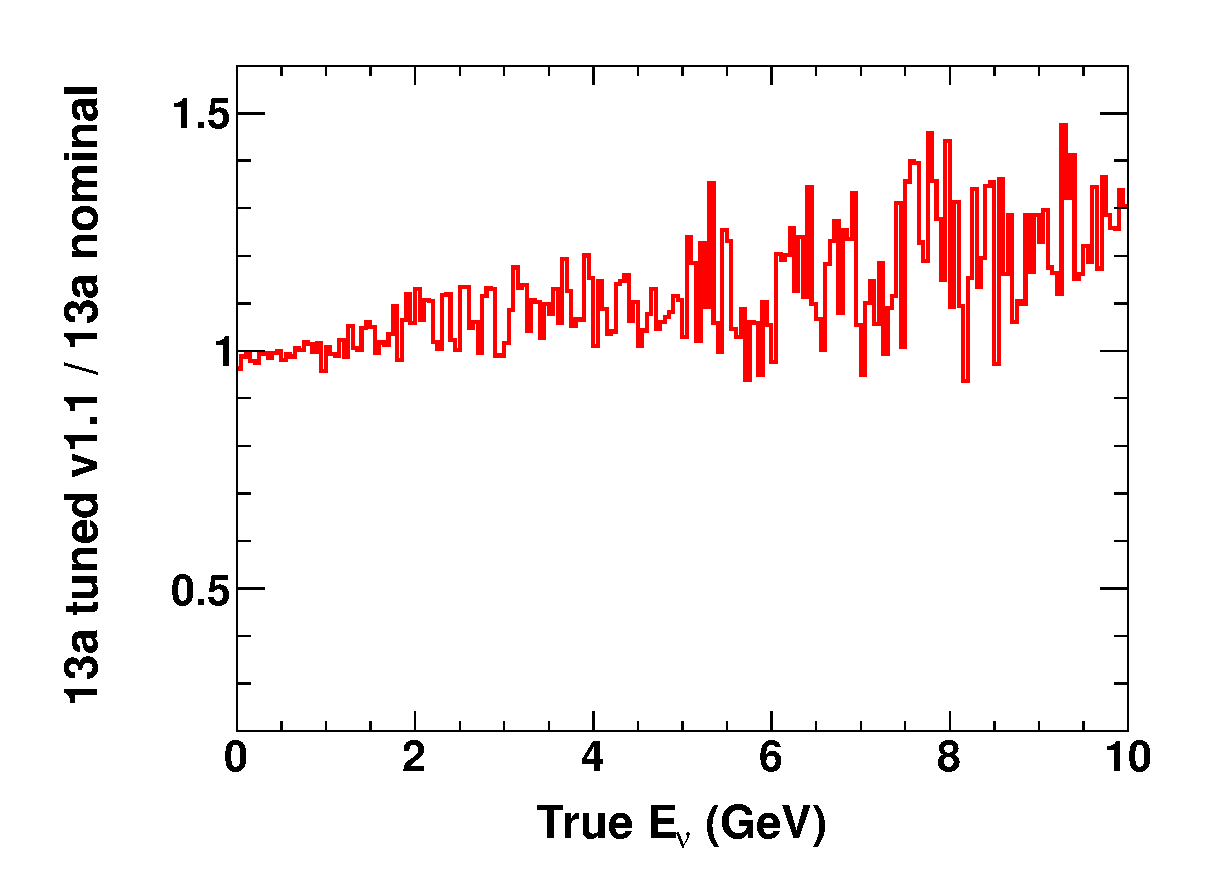
\includegraphics[width=18pc]{./nuebar_plots/spectrum_predictions/flux_ratio_13av1p1_to_13anom_numu.eps}
%
\includegraphics[width=18pc]{./images/missing_plot.eps}
\caption {
  $\nu_\mu$ 13a\_v1.1 Run 5c-6b flux tuning weights applied to nominal $\nu_\mu$ and oscillated-$\nu_e$ MC templates \cite{FluxTuning13a}.
  }
\label{fig:na61_weights:numu}
\end{minipage}
\hspace{0.06\linewidth}
\begin{minipage}[t]{0.48\linewidth}
\center
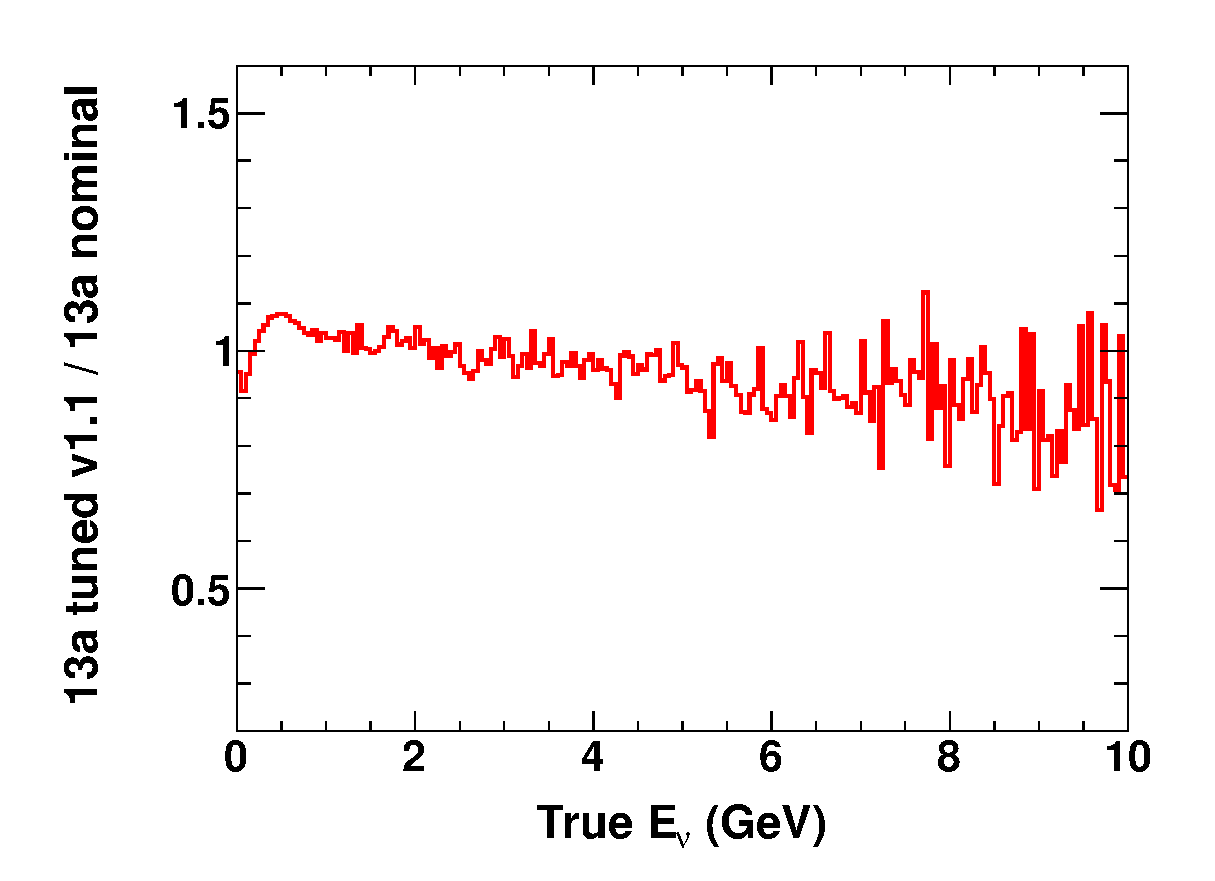
\includegraphics[width=18pc]{./nuebar_plots/spectrum_predictions/flux_ratio_13av1p1_to_13anom_numubar.eps}
%
\includegraphics[width=18pc]{./images/missing_plot.eps}
\caption {
  $\bar{\nu}_\mu$ 13a\_v1.1 Run 5c-6b flux tuning weights applied to nominal $\bar{\nu}_\mu$ and oscillated-$\bar{\nu}_e$ MC templates \cite{FluxTuning13a}.
}
\label{fig:na61_weights:numubar}
\end{minipage}
\vfill
\begin{minipage}[t]{0.48\linewidth}
\center
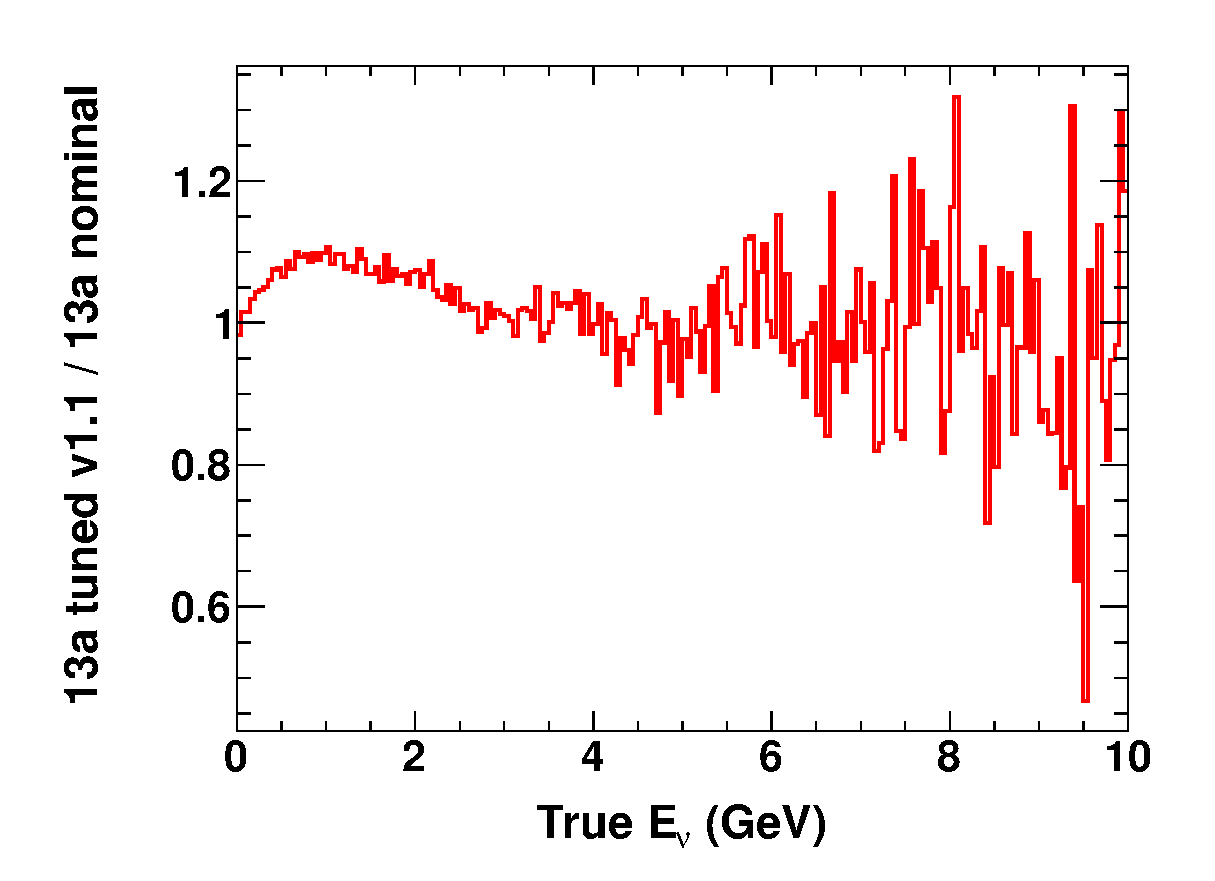
\includegraphics[width=18pc]{./nuebar_plots/spectrum_predictions/flux_ratio_13av1p1_to_13anom_nue.eps}
%
\includegraphics[width=18pc]{./images/missing_plot.eps}
\caption {
  $\nu_e$ 13a\_v1.1\ Run 5c-6b flux tuning weights applied to nominal $\nu_e$ MC templates \cite{FluxTuning13a}.
}
\label{fig:na61_weights:nue}
\end{minipage}
\hspace{0.06\linewidth}
\begin{minipage}[t]{0.48\linewidth}
\center
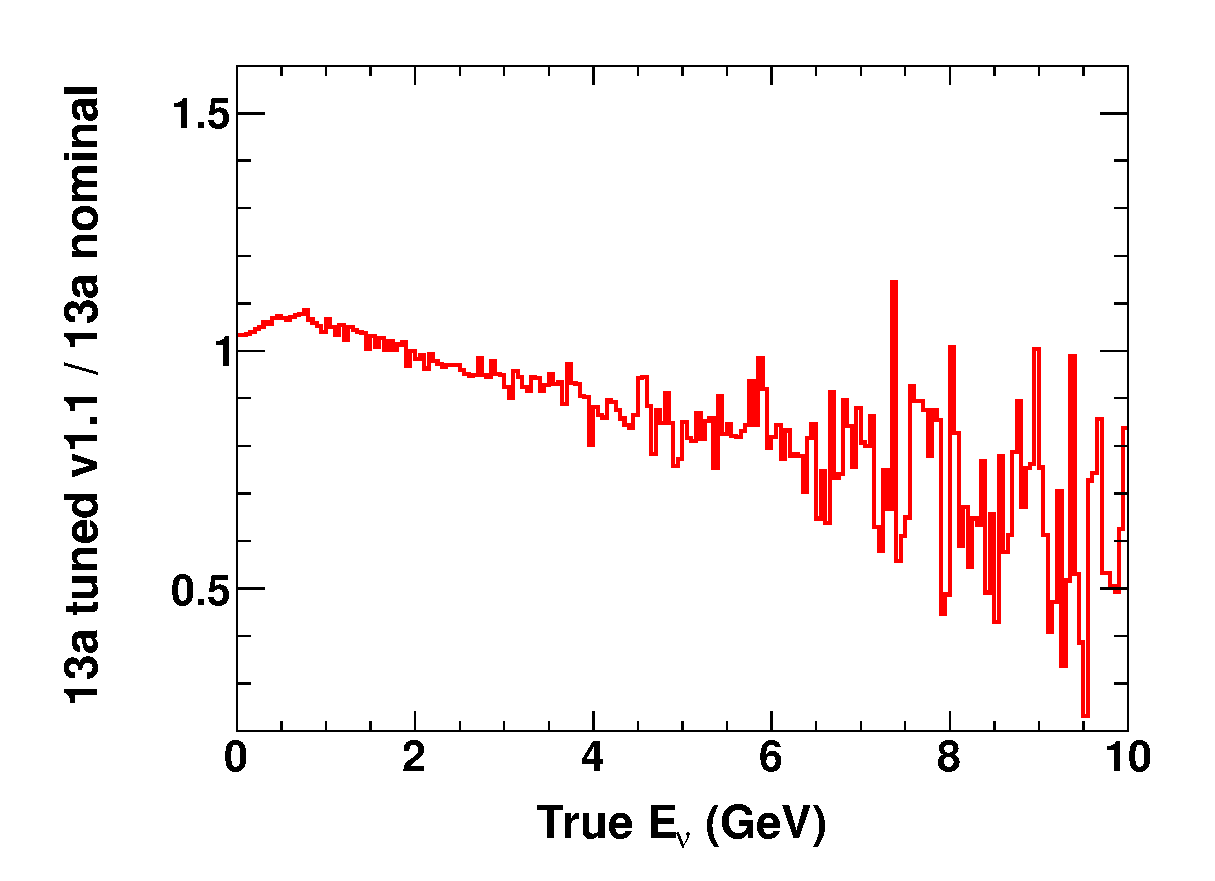
\includegraphics[width=18pc]{./nuebar_plots/spectrum_predictions/flux_ratio_13av1p1_to_13anom_nuebar.eps}
%
\includegraphics[width=18pc]{./images/missing_plot.eps}
\caption {
  $\bar{\nu}_e$ 13a\_v1.1 Run 5c-6b flux tuning weights applied to nominal $\bar{\nu}_e$ MC templates \cite{FluxTuning13a}.
}
\label{fig:na61_weights:nuebar}
\end{minipage}
\end{figure*}

%....................................................................................................................
%....................................................................................................................

\subsection {Applying flux and cross-section (BANFF) tuning based on ND280 data}
\label{sec:banff_weights}

The BANFF group has made a fit of the $\bar{\nu}_\mu$ and  $\nu_\mu$ 
%CC0$\pi$-like, CC1$\pi$-like and CC other 
ND280 samples 
to find the best-fit values of the flux normalisation and cross-section parameters \cite{BANFF2015}. This 
analysis uses these best-fit values to reweight the NA61/SHINE-tuned MC templates, and the templates obtained after this second 
reweighting will be denoted the {\em BANFF-tuned} MC templates in this document.
A list of BANFF parameters, their best-fit values and their 1$\sigma$ prefit and postfit errors is given in 
Tab.~\ref{tab:banff_uncertainties_flux_fhc},~\ref{tab:banff_uncertainties_flux_rhc},
\ref{tab:banff_uncertainties_xsec} and~\ref{tab:banff_uncertainties_skdetfsi}.

The effects of the BANFF tune on the predicted spectra is discussed 
in Sec.~\ref{sec:nominal_and_tuned_predictions}. 
%(see Figs.~\ref{fig:1Re_spectrum_w_and_wo_banff_weights} and Tabs.~\ref{tab:nsk_nominal_no_osc} and~\ref{tab:nsk_nominal_osc}). 
%....................................................................................................................
%....................................................................................................................


\subsection{Applying neutrino oscillations}
\label{sec:applying_oscillations}

The MC templates are constructed from the unoscillated MC samples and must be weighted with the appropriate oscillation 
probability. Oscillations are applied as a function of true energy to the
%  $\bar{\nu}_{\mu}$ CCQE,
%  $\bar{\nu}_{\mu}$ CC1$\pi$,
%  $\bar{\nu}_{\mu}$ CC coherent,
%  $\bar{\nu}_{\mu}$ CC other,
%  $\nu_{\mu}$ CCQE,
%  $\nu_{\mu}$ CC1$\pi$,
%  $\nu_{\mu}$ CC coherent,
%  $\nu_{\mu}$ CC other,
%  $\bar{\nu}_{e}$ CCQE,
%  $\bar{\nu}_{e}$ CC1$\pi$,
%  $\bar{\nu}_{e}$ CC coherent,
%  $\bar{\nu}_{e}$ CC other
%  $\nu_{e}$ CCQE,
%  $\nu_{e}$ CC1$\pi$,
%  $\nu_{e}$ CC coherent,
%  $\nu_{e}$ CC other,
%  oscillated $\bar{\nu}_{\mu} \rightarrow \bar{\nu}_{e}$ CCQE,
%  oscillated $\bar{\nu}_{\mu} \rightarrow \bar{\nu}_{e}$ CC1$\pi$,
%  oscillated $\bar{\nu}_{\mu} \rightarrow \bar{\nu}_{e}$ CC coherent,
%  oscillated $\bar{\nu}_{\mu} \rightarrow \bar{\nu}_{e}$ CC other,
%  oscillated $\nu_{\mu} \rightarrow \nu_{e}$ CCQE,
%  oscillated $\nu_{\mu} \rightarrow \nu_{e}$ CC1$\pi$,
%  oscillated $\nu_{\mu} \rightarrow \nu_{e}$ CC coherent,
%  oscillated $\nu_{\mu} \rightarrow \nu_{e}$ CC other,
%  oscillated $\nu_{e} \rightarrow \nu_{\mu}$ CCQE,
%  oscillated $\nu_{e} \rightarrow \nu_{\mu}$ CC1$\pi$,
%  oscillated $\nu_{e} \rightarrow \nu_{\mu}$ CC coherent and
%  oscillated $\nu_{e} \rightarrow \nu_{\mu}$ CC other
  MC templates for all CC interactions.

The MC templates calculated from the $\overset{\scriptscriptstyle{(-)}}{\nu_\mu}$ MC sample are weighted 
with P($\overset{\scriptscriptstyle{(-)}}{\nu_\mu} \rightarrow \overset{\scriptscriptstyle{(-)}}{\nu_\mu}$), with this survival probability being calculated using the 
oscillation parameters, namely $\sin^{2} \theta_{23}$, $\sin^{2} \theta_{12}$, $\sin^{2} \theta_{13}$, 
$|\Delta m^{2}_{32}|$ (normal hierarchy) or $|\Delta m^{2}_{31}|$ (inverted hierarchy), 
$\Delta m^{2}_{21}$ and $\delta_{CP}$. The $\overset{\scriptscriptstyle{(-)}}{\nu_e}$ templates are weighted with P($\overset{\scriptscriptstyle{(-)}}{\nu_e} \rightarrow \overset{\scriptscriptstyle{(-)}}{\nu_e}$), 
while the oscillated $\overset{\scriptscriptstyle{(-)}}{\nu_\mu} \rightarrow \overset{\scriptscriptstyle{(-)}}{\nu_e}$ templates are weighted with P($\overset{\scriptscriptstyle{(-)}}{\nu_\mu} \rightarrow \overset{\scriptscriptstyle{(-)}}{\nu_e}$) 
(the sample was generated assuming 100\% of $\overset{\scriptscriptstyle{(-)}}{\nu_\mu}$ transform to $\overset{\scriptscriptstyle{(-)}}{\nu_e}$). 
%The $\nu_{\mu}$ templates are weighted with P($\nu_{\mu}\rightarrow\nu_{\mu}$). 
%The $\nu_{e}$ templates are weighted with P($\nu_{e}\rightarrow\nu_{e}$) and the 
%oscillated $\nu_{\mu} \rightarrow \nu_{e}$ templates with P($\nu_{\mu}\rightarrow\nu_{e}$).
All these oscillation probabilities are computed in a 3-flavour framework including matter effects in constant-density matter
(assuming an Earth crust density of 2.6 g/cm$^{3}$).
Custom oscillation probability calculation code was developed within the {\em VALOR} analysis framework.
Details and estimates of the numerical accuracy of this code are first presented in \cite{OurRun12DisappAnalysis3Flavour},
and is also shown in Appendix A of \cite{OurRun123DisappAnalysis3Flavour}.
Comparisons between the {\em VALOR} oscillation probability calculation code and Prob3++ \cite{Prob3}, 
which is typically used by the alternative T2K oscillation analyses, are shown in Appendix B of \cite{OurRun123DisappAnalysis3Flavour}.

In the standard 3-flavour oscillation framework,
oscillations of $\overset{\scriptscriptstyle{(-)}}{\nu_e}$ and $\overset{\scriptscriptstyle{(-)}}{\nu_\mu}$ can yield $\overset{\scriptscriptstyle{(-)}}{\nu_\tau}$.
In this analysis, we neglect contributions from $\nu_{\tau}$-CC and $\bar{\nu}_{\tau}$-CC as their
energy threshold is around 3.5 GeV and their effect is negligible\footnote{
A back-of-the-envelope calculation can be found in the replies to
comments and revision history document of
\cite{OurRun123DisappAnalysis3Flavour} that gives $\ll 1\%$ $\nu_\tau$
contamination in the 1-ring $\mu$-like Super-K sample. A Super-K MC study is required
to determine whether the Super-K efficiency assumptions made there are valid.
  }.
Accordingly, this analysis uses no $\nu_{\tau}$-CC and $\bar{\nu}_{\tau}$-CC MC templates
(and, in fact, no $\nu_{\tau}$ and $\bar{\nu}_{\tau}$ Super-K MC samples are available).

It should be emphasized here that
the $\nu_{\mu}$ NC MC templates for a mode $m$ are proxies for the
NC MC templates for the mixture of $\nu_{e}$+$\nu_{\mu}$+$\nu_{\tau}$ resulting from
3-flavour $\nu_{\mu}$ oscillations for that mode $m$. The same applies to the $\bar{\nu}_{\mu}$, $\nu_{e}$ and $\bar{\nu}_{e}$ 
NC MC templates. These NC MC templates are unchanged under standard 3-flavour oscillations.% (see also Sec.~\ref{sec:}).

Also it should be noted that there are no explicit NC MC templates made from the oscillated $\bar{\nu}_{e}$ and $\nu_{e}$ 
samples. If they were used, the oscillated $\bar{\nu}_{e}$ (i.e.\ $\bar{\nu}_{e}$ coming from oscillations of $\bar{\nu}_{\mu}$) 
would be double counted since they are already included in the $\bar{\nu}_{\mu}$ NC MC templates. The same applies to oscillated 
$\nu_{e}$.

%....................................................................................................................
%....................................................................................................................

\subsection {Predictions of nominal and tuned-MC spectra}
\label{sec:nominal_and_tuned_predictions}

In this section, we present the expected spectra in Super-K for various oscillation scenarios. 
%We also present estimates of the effect of the NA61/SHINE and BANFF tunings and of assumptions 
%made in the 3-flavour neutrino oscillation framework used in this analysis. 
Unless explicitly stated otherwise, the oscillation 
parameters are set to the values shown in Tab.~\ref{tab:osc_params_joint_asimov} and the normal mass hierarchy is assumed.
All plots are generated for an integrated exposure of 
\TotalPotNu{} POT for neutrino and \TotalPotNuBar{} POT for antineutrino mode.


Predicted single ring Super-K spectra are shown in Fig.~\ref{fig:joint_ereco_vs_theta_all}. 
By comparing neutrino and antineutrino mode $e$-like plots it is clear that $E_{reco}$ Vs $\theta$ distributions are differently populated
by $\nu_{\mu} \rightarrow \nu_e$ and $\bar{\nu}_{\mu} \rightarrow \bar{\nu}_e$ events.
More details on the advantage of the 2-dimensional templates are given in App.~\ref{app:templates_elike}.

%for oscillations assuming the normal hierarchy and the oscillation parameters shown in table~\ref{tab:osc_params_joint}.

\begin{figure*}[htb]
\center
\begin{subfigure}[b]{0.49\textwidth}
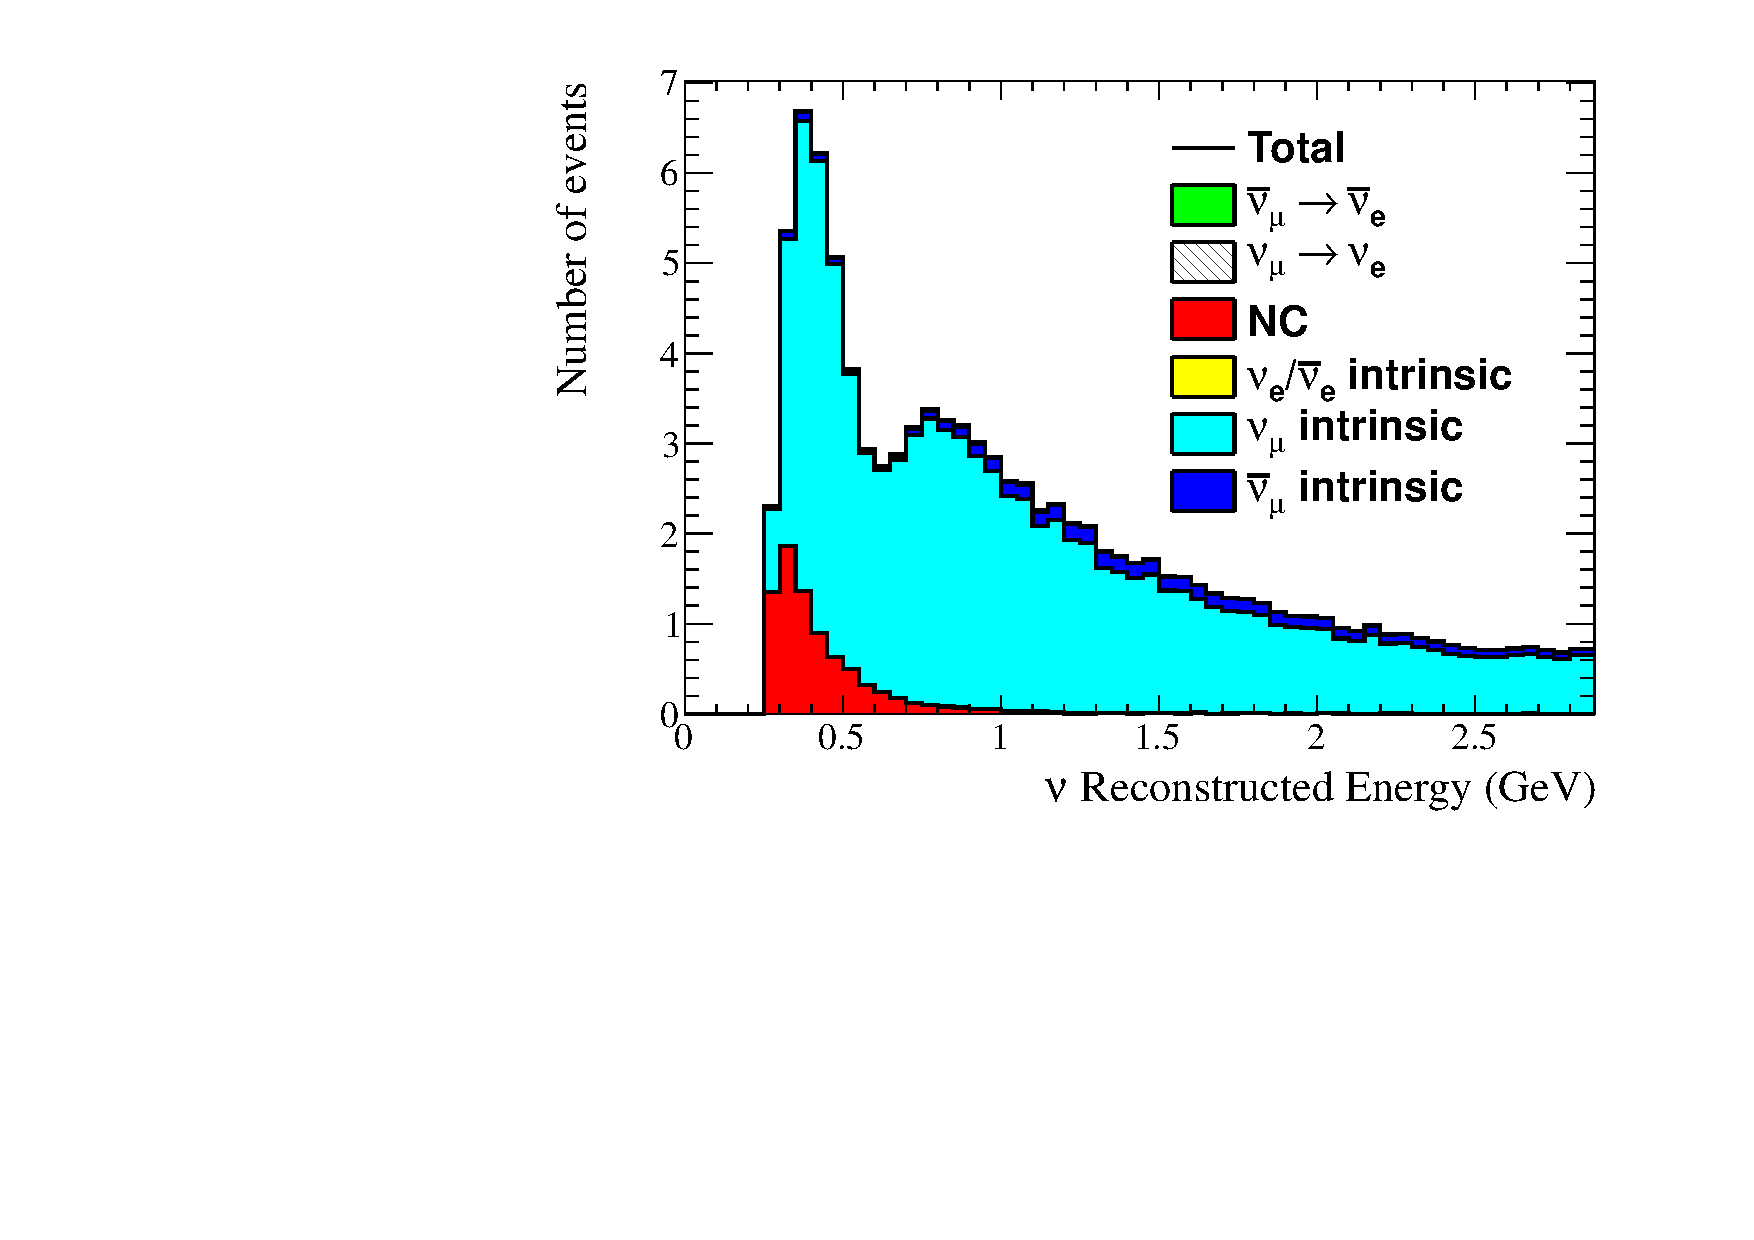
\includegraphics[width=0.9\textwidth]{joint_plots/spectrum_predictions/template_ereco_1rmu_zoom.pdf}
\caption{Muon-like, neutrino mode}
\end{subfigure}
\begin{subfigure}[b]{0.49\textwidth}
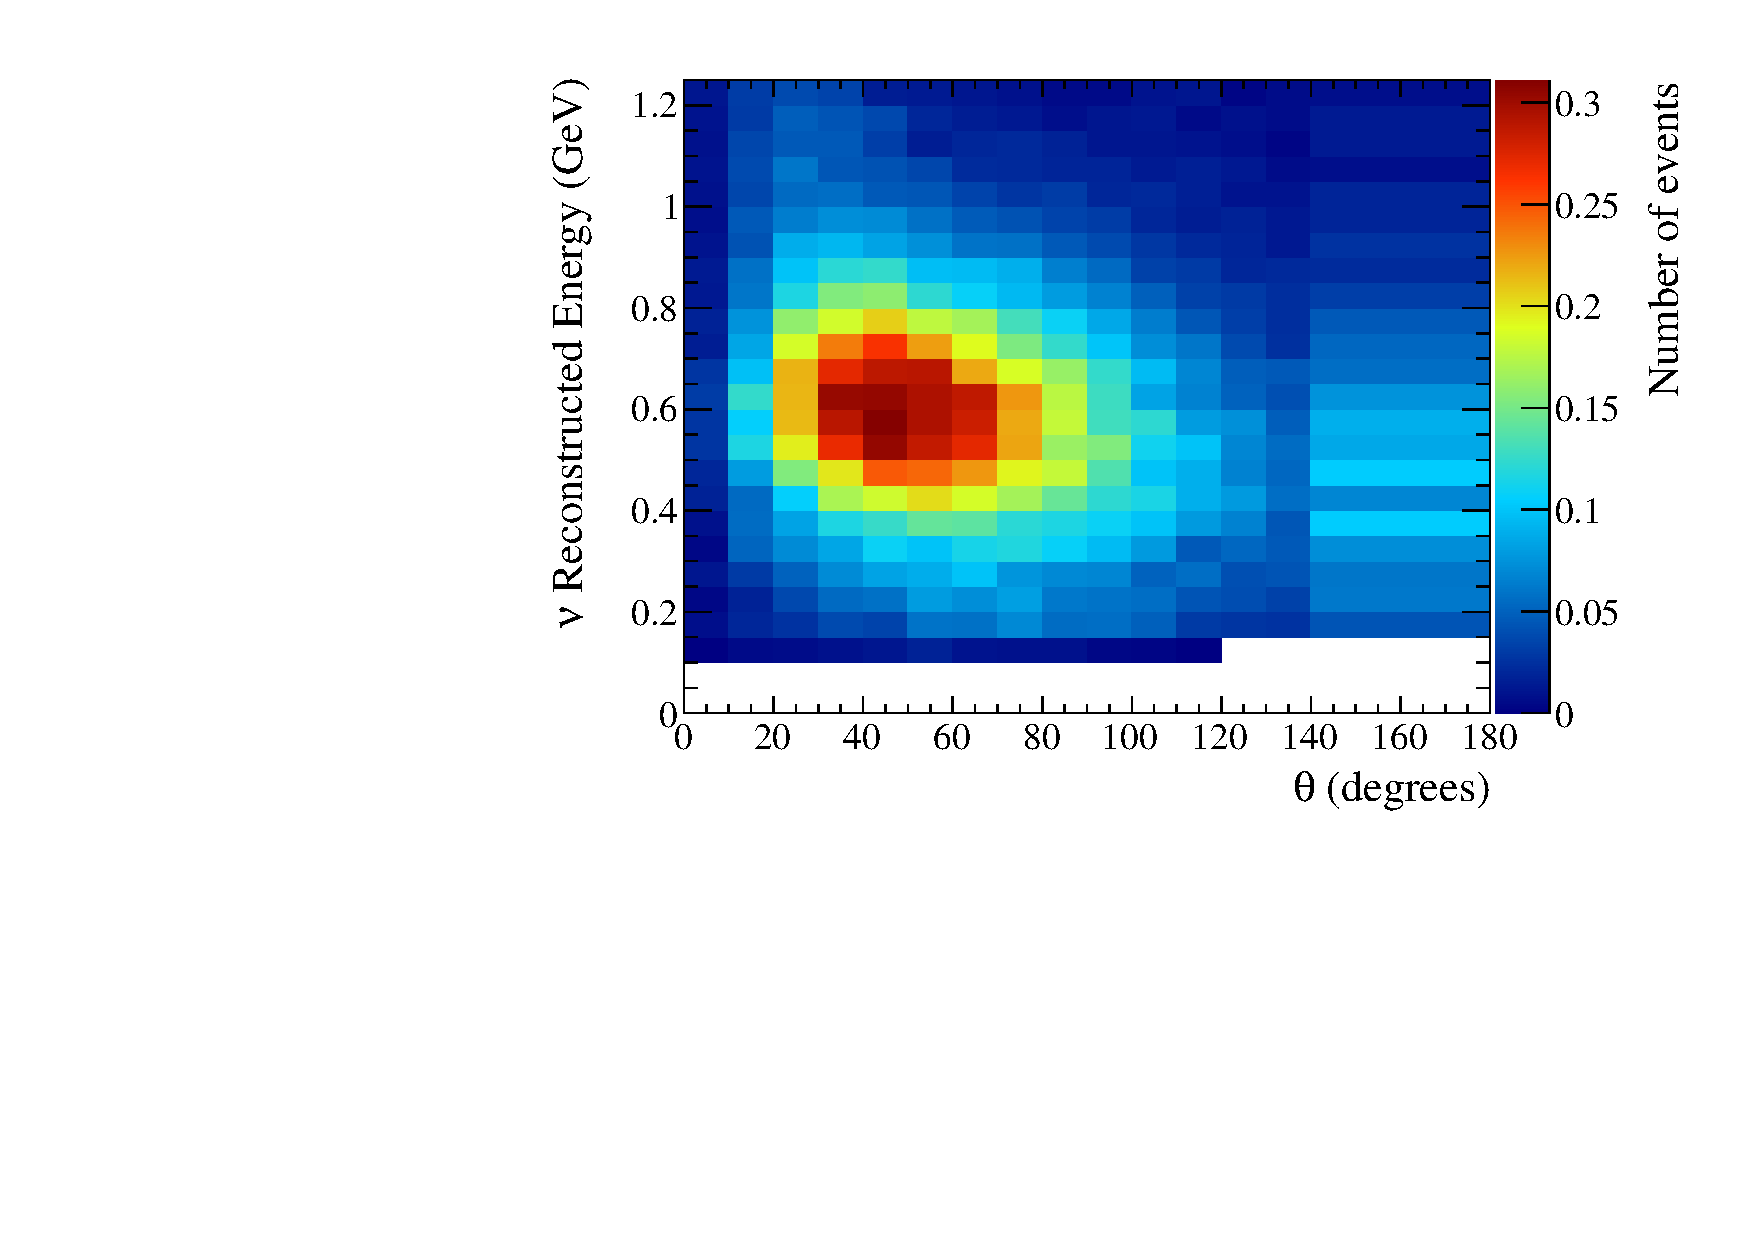
\includegraphics[width=0.9\textwidth]{joint_plots/spectrum_predictions/template_ereco_vs_theta_tot_1re.pdf}
\caption{Electron-like, neutrino mode}
\end{subfigure}
\begin{subfigure}[b]{0.49\textwidth}
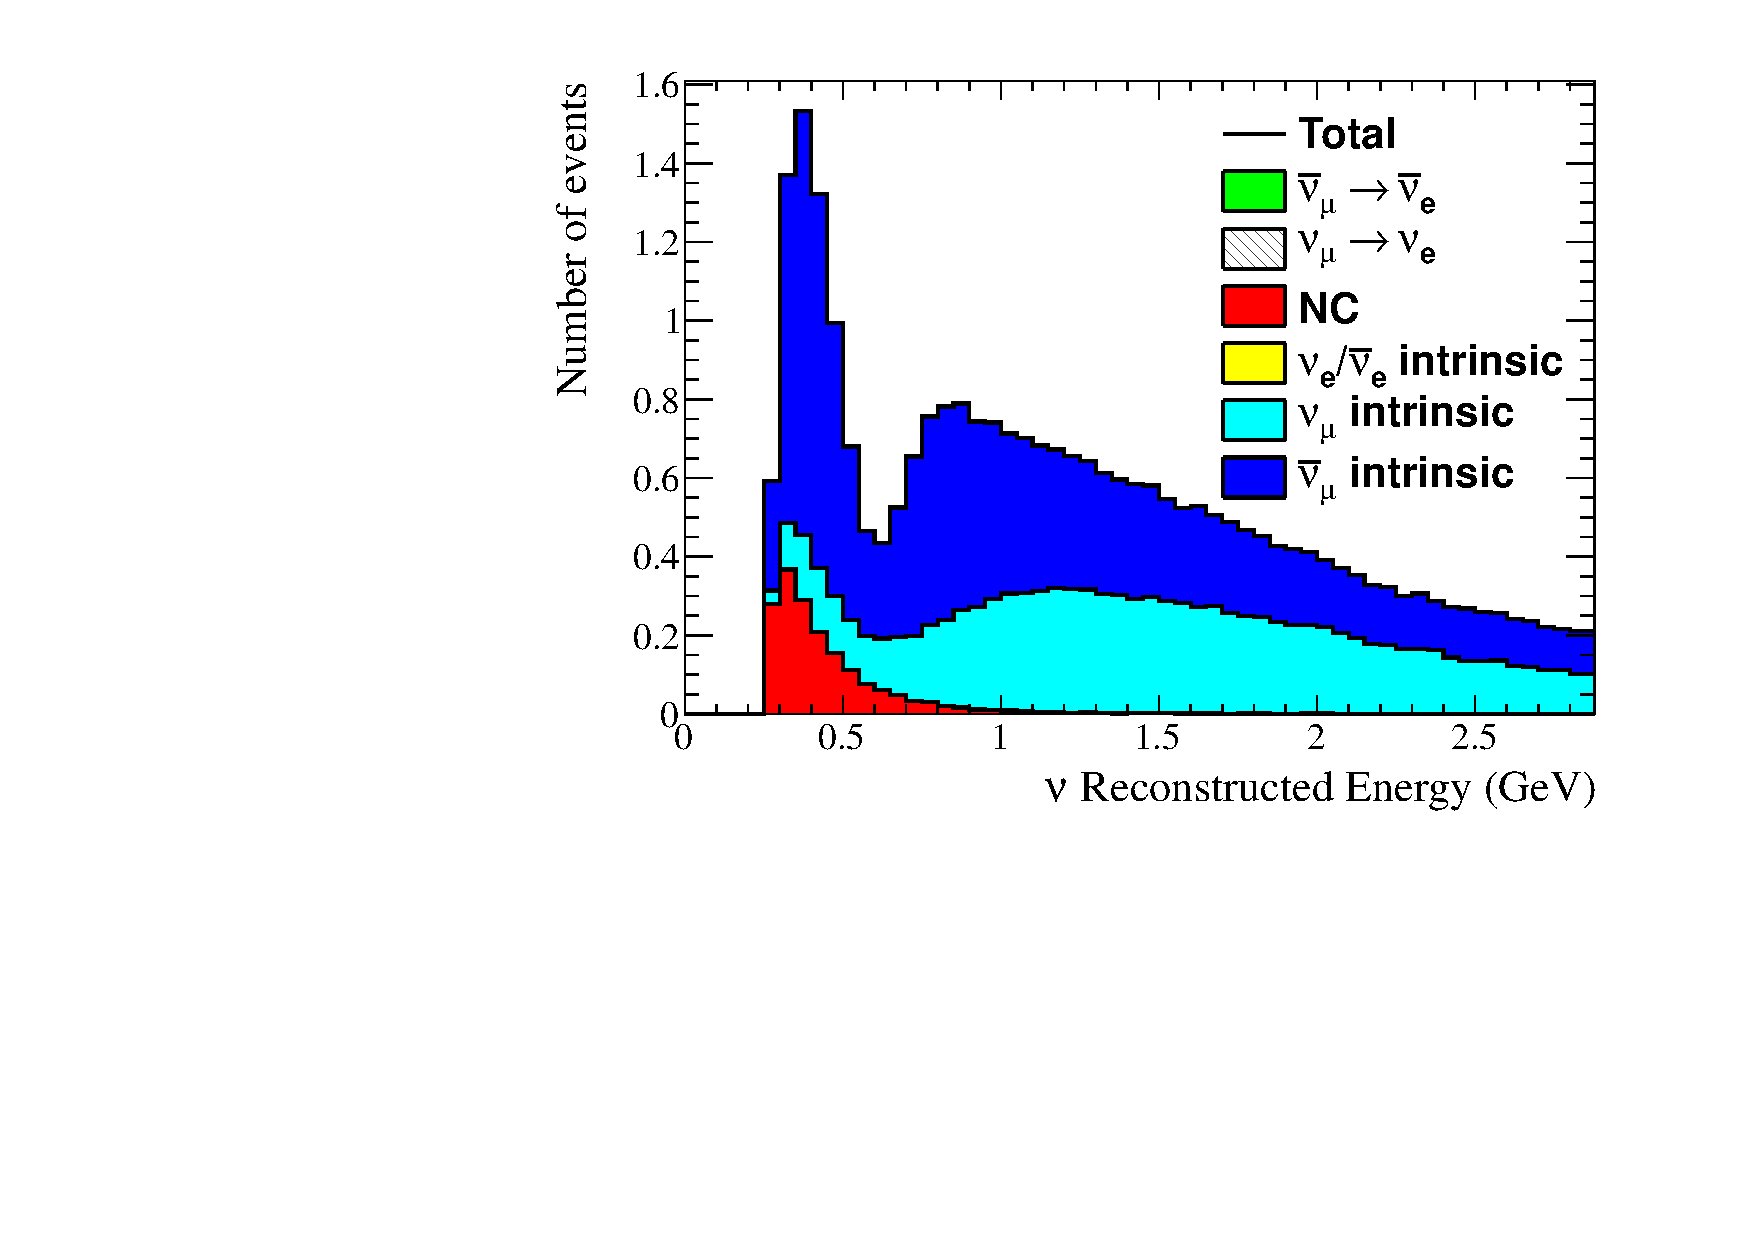
\includegraphics[width=0.9\textwidth]{joint_plots/spectrum_predictions/template_ereco_rhc1rmu_zoom.pdf}
\caption{Muon-like, antineutrino mode}
\end{subfigure}
\begin{subfigure}[b]{0.49\textwidth}
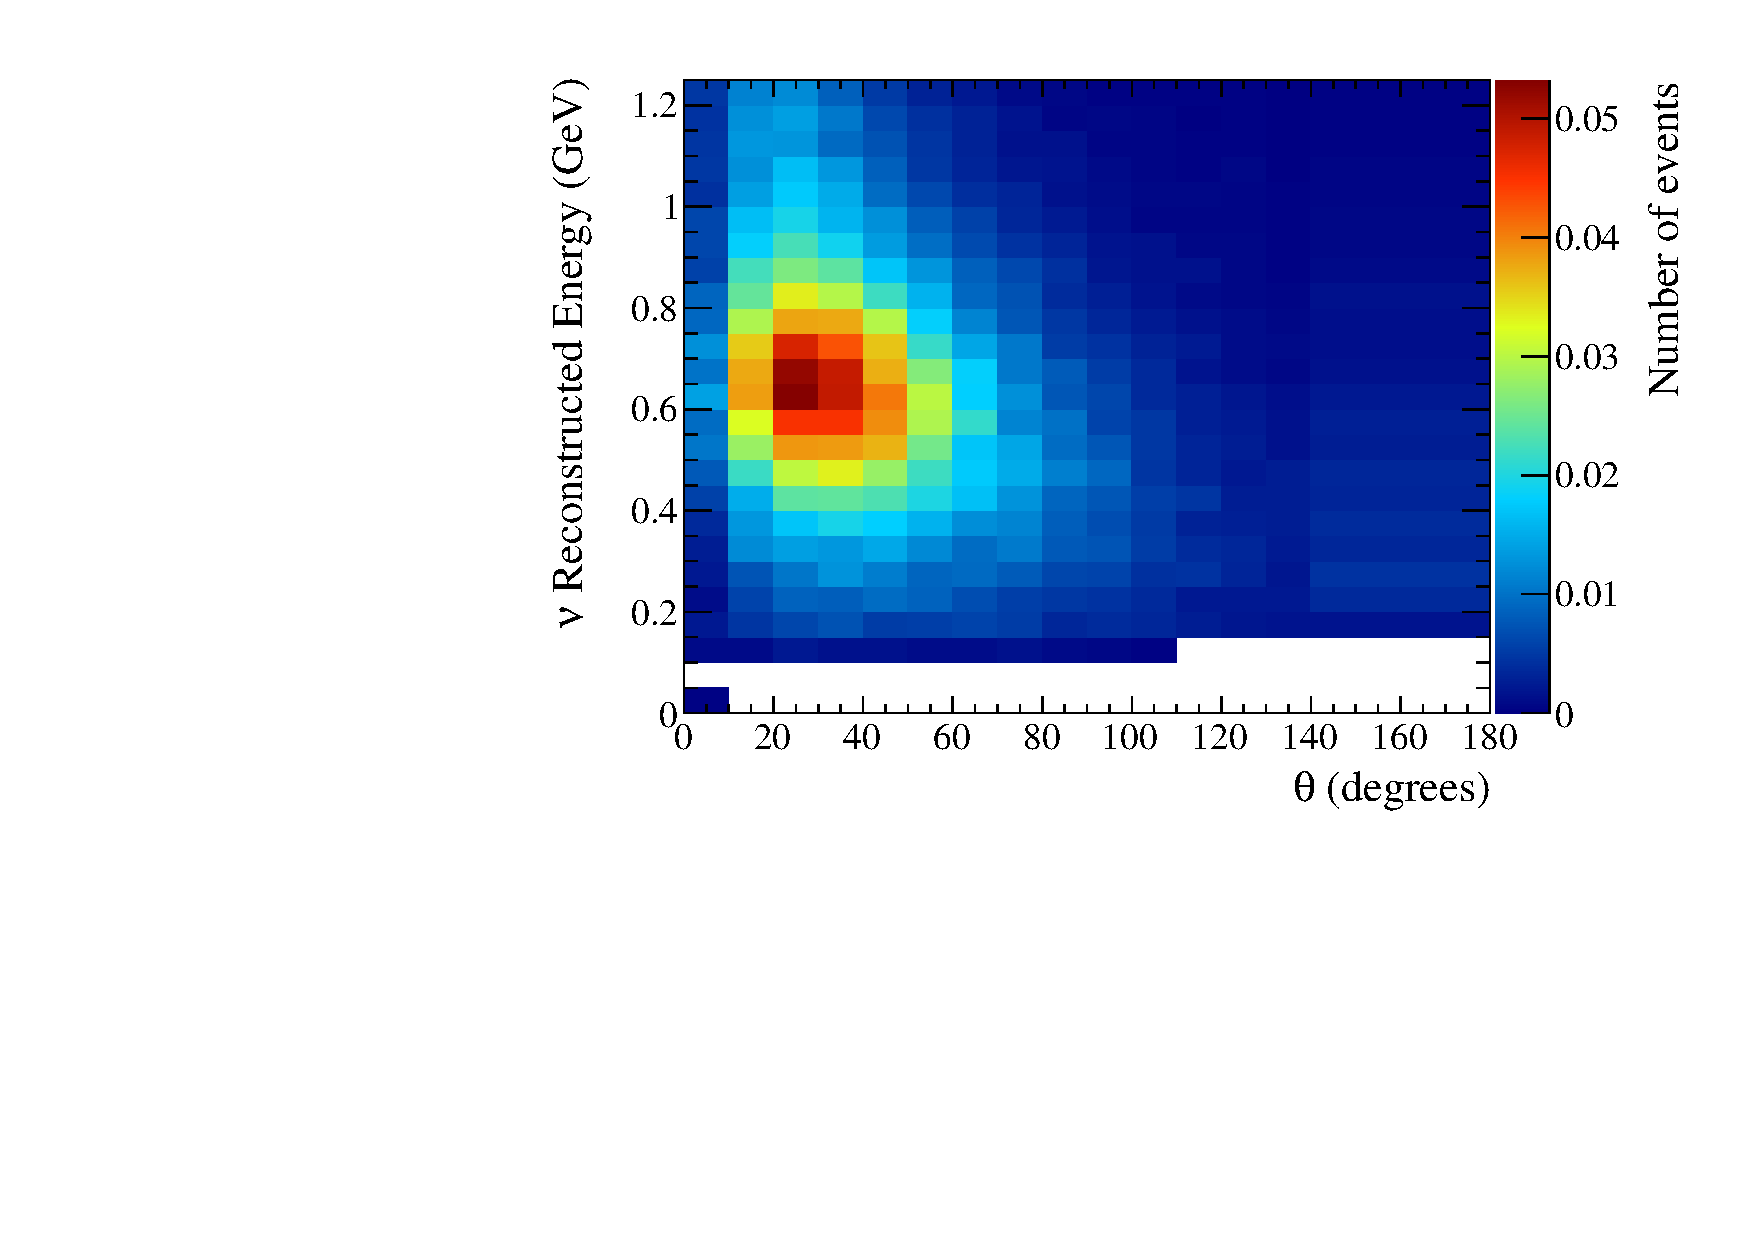
\includegraphics[width=0.9\textwidth]{joint_plots/spectrum_predictions/template_ereco_vs_theta_tot_rhc1re.pdf}
\caption{Electron-like antineutrino mode}
\end{subfigure}
\caption {
Predicted spectra, muon-like distributions are function of the reconstructed neutrino energy,
while the electron-like distributions are function of both the reconstructed neutrino energy and
the angle between the outgoing lepton and the neutrino direction.
The distributions correspond to the statistics collected in the full run 1-6 data set
for an exposure 
of $6.914 \times 10^{20}$ POT in neutrino mode
and
of $4.011 \times 10^{20}$ POT in antineutrino mode.
The muon-like distributions are broken down by the following components:
$\bar{\nu}_{\mu} \to \bar{\nu}_e$ (green), 
$\nu_{\mu} \to \nu_e$ (black/white), 
NC (red),
$\nu_e + \bar{\nu}_e$ intrinsic beam (yellow),
$\nu_{\mu}$ intrinsic beam (light blue)
and
$\bar{\nu}_{\mu}$ intrinsic beam (blue).
The spectra are generated with the systematic parameters measured with the ND280 data 
shown in 
Tab.~\ref{tab:banff_uncertainties_flux_fhc},~\ref{tab:banff_uncertainties_flux_rhc},
\ref{tab:banff_uncertainties_xsec} and~\ref{tab:banff_uncertainties_skdetfsi}
and the oscillation parameters corresponding to the Asimov data set A 
shown in tab.~\ref{tab:osc_params_joint_asimov}.
}
\label{fig:joint_ereco_vs_theta_all}
\end{figure*}















%A MC tune derived using NA61/SHINE data is applied to the nominal MC templates, and another tune derived using the ND280 data is 
%applied to the NA61/SHINE-tuned templates as described in Secs.~\ref{sec:na61_weights} and~\ref{sec:banff_weights}.
%%
%The fractional difference in the expected number of single $e$-like ring events when switching from the nominal MC to the
%NA61/SHINE-tuned MC templates is shown in Fig.~\ref{fig:1Re_spectrum_w_and_wo_na61_weights} 
%both oscillated and not oscillated. 
%%In Fig.~\ref{fig:1Re_spectrum_w_and_wo_banff_weights} it is shown the fractional difference in the expected number of
%%single-ring $e$-like events when switching from the NA61/SHINE-tuned MC templates to the BANFF-tuned MC templates.
%In Fig.~\ref{fig:1Re_spectrum_w_and_wo_na61_weights} it is shown the fractional difference in the expected number of single-ring e-like events
%when switching from the nominal MC templates to NA61/SHINE-tuned MC templates.
%%
%The effects of the NA61/SHINE and BANFF tunes on the total expected number of single-ring $e$-like events
%and on the numbers in each of the \NMCTemplate{} component interaction modes are shown in
%Tab.~\ref{tab:nsk_nominal_no_osc} for no oscillations, and in
%Tab.~\ref{tab:nsk_nominal_osc} for oscillations assuming the normal hierarchy, and the oscillation parameters shown in table~\ref{tab:osc_params_fixed_values_reactor}.
%Finally, the effects of the NA61/SHINE and BANFF tunes on the reconstructed energy spectrum of
%single $e$-like ring events are shown in
%Figs.~\ref{fig:1Re_spectrum_w_and_wo_banff_weights}.
%In each case, spectra are shown for both no oscillations and for oscillations assuming the normal hierarchy, and the oscillation parameters shown in table~\ref{tab:osc_params_fixed_values_reactor}.
%%Also shown are the ratio of flux-tuned spectrum to nominal spectrum, and
%%BANFF-tuned spectrum to flux-tuned spectrum in Figs.~\ref{fig:1Re_spectrum_w_and_wo_banff_weights}.
%Also shown are the ratio of BANFF-tuned spectrum to flux-tuned spectrum in Figs.~\ref{fig:1Re_spectrum_w_and_wo_banff_weights}.


\clearpage

\section {Systematic effects in the prediction of the single $\mu$-like ring event energy spectrum}
\label{sec:systematics}

%....................................................................................................................
%....................................................................................................................

\subsection {Input systematic parameters}

\label{sec:systematics:inputs}

This analysis considers \NSyst{} systematic parameters which can be grouped into 4 categories:

\begin{enumerate}

\item 
{\bf Flux and cross-section parameters} (65 parameters).\\

In this analysis, all the flux and cross-section systematic parameters are included in the ND280 data (BANFF) fit.
However, since ND280 is not sensitive to some cross section systematics they remain unconstrained
(detailed later).
Parameters fit are 
11 $\nu_{\mu}$, 5 $\bar{\nu}_{\mu}$, 7 $\nu_{e}$ and 2 $\bar{\nu}_{e}$ neutrino mode (FHC) flux parameters, 
5 $\nu_{\mu}$, 11 $\bar{\nu}_{\mu}$, 2 $\nu_{e}$ and 7 $\bar{\nu}_{e}$ antineutrino mode (RHC) flux parameters 
and 15 cross-section parameters. 
Best-fit values of these parameters and a covariance matrix giving their correlated uncertainties are obtained by the BANFF group from a fit 
of the $\bar{\nu}_\mu$ and $\nu_\mu$ 
%CC0$\pi$-like, CC1$\pi$-like and CC other-like 
ND280 samples as described in Ref~\cite{BANFF2015}. 
A list of the BANFF parameters, their best-fit values and their prefit and postfit errors is given in 
Tab.~\ref{tab:banff_uncertainties_flux_fhc},~\ref{tab:banff_uncertainties_flux_rhc},
\ref{tab:banff_uncertainties_xsec} and~\ref{tab:banff_uncertainties_skdetfsi}.
The best-fit values are used to reweight the templates as described in Sec.~\ref{sec:banff_weights}, and the postfit errors in the 
covariance matrix are used as prior uncertainties in this analysis. 

The effects of these correlated uncertainties are evaluated using the Cholesky method,
that allows to throw the systematic parameters according to their multivariate distribution
taking into account the existing correlations.
%The covariance matrix is ``Cholesky decomposed'' 
%into the product of a lower triangular matrix (all elements above the diagonal are zero) and its transpose (in which all elements below the 
%diagonal are zero). Random tweaks of each parameter are independently drawn from a Gaussian distribution with mean zero and standard deviation 1, 
%and these random numbers are put into a vector. This vector is then multiplied by the lower triangular matrix to give a vector of tweaked 
%uncertainties that have the correct correlations between them. The BANFF parameters are then varied by these tweaked uncertainties, with all 
%parameters being varied simultaneously. This process may be repeated as many times as necessary. 

Some of the cross-section parameters have a complicated, often non-linear, effects on true and reconstructed neutrino energy bin normalisations; 
the effects of uncertainties in these parameters are evaluated by reweighting the MC templates. Weights are calculated for tweaks from -3$\sigma$ to +3$\sigma$ 
in steps of 0.5$\sigma$, and interpolations are made between those weights using cubic splines (for MaQE only, weights are calculated from 
-7$\sigma$ to +3$\sigma$). Cubic splines are made for the following cross-section uncertainties:
\begin{itemize}
\item CCQE axial-mass scaling factor (MaQE)
\item Fermi momentum for $^{16}$O
\item Binding energy for $^{16}$O
\item Nucleon to $\Delta$ transition axial form factor (C$^{A}_{5}$) 
\item Resonance-production axial-mass scaling factor (MaRes)
\item Scale of isospin 1/2 nonresonant background
\item CC other shape
\end{itemize}
The splines are made in bins of theta, true and reconstructed energy, and the binning is given in Ref.\ \cite{splineinfo}.

The effects of the flux and cross-section normalization uncertainties are also evaluated by reweighting the MC templates, but no splines are made for them
since the weight is identical to the tweak for these uncertainties (each flux parameter is a normalization for a limited range of true energy). 
The cross section parameters which simply normalise the overall spectrum component are:
\begin{itemize}
\item MEC, applied to all the MEC events (both neutrino and antineutrino)
\item MEC-$\bar{\nu}$, applied to all the antineutrino MEC events
\item CC coherent for $^{16}$O normalisation                     
\item NC coherent normalisation                                       
\item NC other normalisation                                           
\item NC $1\gamma$ normalisation                                          
\item CC $\nu_{e}$ normalisation                                  
\item CC $\bar{\nu}_{e}$ normalisation                                  
\end{itemize}

Uncertainties due to  ``second class currents" are implemented as an additional uncertainty on CC $\bar{\nu}_{e}$ and CC $\nu_{e}$ parameters
with a 2\% anti-correlated constraint between them.
The BANFF parameters are applied to the MC templates as specified in 
Tab.~\ref{tab:apply_syst_to_template_mulike_fhc},
~\ref{tab:apply_syst_to_template_elike_fhc},
~\ref{tab:apply_syst_to_template_mulike_rhc} and
~\ref{tab:apply_syst_to_template_elike_rhc}.
The normalisation parameter of the NC$1\gamma$ component was not used in the previous analyses,
since it was included in NC other.

In the BANFF fit a bias on the best-fit flux parameters is present due to the degeneracy 
between the neutrino flux and ND280 detector parameters.
For this reason a covariance matrix that accounts for the bias of the flux as well as all the other parameters is summed in quadrature
to the total post-fit covariance. Furthermore the best-fit values have been corrected in order to remove the bias. 
The description of the procedure is given in \cite{BANFF2015}.
As shown in \cref{app:systematics} the impact of the bias on the systematic parameters fitted by the BANFF analysis is small
compared to the other systematic uncertainties.


The predicted number of events in antineutrino mode $e$-like sample is now smaller compared to the $\bar{\nu}_e$ appearance analysis  
presented at the 2015 summer conferences
\cite{OurRun56AntiNueBarAppearanceAnalysis3Flavour},
3.218 instead of 3.729.
The differences between the current and previous oscillation analyses is mainly due to:

\begin{enumerate}

\item new value of $\sin^2 \theta_{13}$ corresponding to the PDG 2015 release, as shown in Tab.~\ref{tab:osc_params_joint_asimov},
	which is 0.0217 while in the previous analysis it was 0.0250. If the old PDG value is used the expected number of 
	antineutrino mode $e$-like events becomes 3.542.

\item Subsequently, if the cross section parameters are set to the old post-BANFF fit values, the expected number of events becomes 3.63. 
	Indeed all the post-BANFF 2015 fit cross section parameters are higher compared to the 2016 BANFF fit result. 
	The effect of the flux parameters is smaller, indeed if they are set to BANFF 2015 result, the expected number of events becomes 3.66.
 
\item Finally, after all the changes listed above,
	the rescaling of CC coherent and NC$1\gamma$ components (see \ref{sec:mc_templates:input_mc}) is not applied, 
	the agreement between the 2015 and 2016 analysis is obtained.
	The first one increases the number of events up to 3.772 while the latter one reduces down to 3.711, which is approximately 
	the number of events expected in the 2015 analysis. 

%\item the total normalization for MEC events for antineutrinos is 0.894,   �  
%	where the BANFF best-fit of the MEC parameter applied only to $\bar{\nu}$ is $0.578$ and 
%	the best-fit of the MEC parameter applied to all the flavors is 1.546.
%	 This reduces the expected total number 
%	of $\bar{\nu}_e$ events, while in the past analysis a single systematic parameter was applied to all the MEC events 
%	and its BANFF best-fit was about 1.031.

\end{enumerate}


{
\renewcommand{\arraystretch}{1.2}
\begin{table}
\centering
\begin{tabular}{| c | c | c | c |}
\hline
           Parameter & Description & Best fit & 1$\sigma$ pre/postfit \\
           & & & fractional error \\
\hline
            0 &  $\nu_{\mu}$ flux normalisation, E = 0.0 - 0.7 GeV               & 1.142   & 0.094 / 0.071 \\ 
            1 &  $\nu_{\mu}$ flux normalisation, E = 0.7 - 1.0 GeV               & 1.091   & 0.079 / 0.053 \\ 
            2 &  $\nu_{\mu}$ flux normalisation, E = 1.0 - 1.5 GeV               & 1.079   & 0.077 / 0.052 \\ 
            3 &  $\nu_{\mu}$ flux normalisation, E = 1.5 - 2.5 GeV               & 1.074   & 0.081 / 0.060 \\ 
            4 &  $\nu_{\mu}$ flux normalisation, E = 2.5 - 30.0 GeV              & 1.050   & 0.080 / 0.053 \\ 
            5 &  $\bar{\nu}_{\mu}$ flux normalisation, E = 0.0 - 0.4 GeV         & 1.204   & 0.104 / 0.069 \\ 
            6 &  $\bar{\nu}_{\mu}$ flux normalisation, E = 0.4 - 0.5 GeV         & 1.210   & 0.102 / 0.058 \\ 
            7 &  $\bar{\nu}_{\mu}$ flux normalisation, E = 0.5 - 0.6 GeV         & 1.180   & 0.096 / 0.051 \\ 
            8 &  $\bar{\nu}_{\mu}$ flux normalisation, E = 0.6 - 0.7 GeV         & 1.128   & 0.085 / 0.041 \\ 
            9 &  $\bar{\nu}_{\mu}$ flux normalisation, E = 0.7 - 1.0 GeV         & 1.123   & 0.125 / 0.077 \\ 
           10 &  $\bar{\nu}_{\mu}$ flux normalisation, E = 1.0 - 1.5 GeV         & 1.118   & 0.105 / 0.068 \\ 
           11 &  $\bar{\nu}_{\mu}$ flux normalisation, E = 1.5 - 2.5 GeV         & 1.121   & 0.080 / 0.053 \\ 
           12 &  $\bar{\nu}_{\mu}$ flux normalisation, E = 2.5 - 3.5 GeV         & 1.121   & 0.074 / 0.049 \\ 
           13 &  $\bar{\nu}_{\mu}$ flux normalisation, E = 3.5 - 5.0 GeV         & 1.122   & 0.094 / 0.067 \\ 
           14 &  $\bar{\nu}_{\mu}$ flux normalisation, E = 5.0 - 7.0 GeV         & 1.112   & 0.093 / 0.064 \\ 
           15 &  $\bar{\nu}_{\mu}$ flux normalisation, E = 7.0 - 30.0 GeV        & 1.093   & 0.130 / 0.108 \\ 
           16 &  $\nu_{e}$ flux normalisation, E = 0.0 - 2.5 GeV                 & 1.109   & 0.069 / 0.047 \\ 
           17 &  $\nu_{e}$ flux normalisation, E = 2.5 - 30.0 GeV                & 1.090   & 0.085 / 0.067 \\ 
           18 &  $\bar{\nu}_{e}$ flux normalisation, E = 0.0 - 0.5 GeV           & 1.193   & 0.095 / 0.054 \\ 
           19 &  $\bar{\nu}_{e}$ flux normalisation, E = 0.5 - 0.7 GeV           & 1.184   & 0.091 / 0.047 \\ 
           20 &  $\bar{\nu}_{e}$ flux normalisation, E = 0.7 - 0.8 GeV           & 1.167   & 0.091 / 0.049 \\ 
           21 &  $\bar{\nu}_{e}$ flux normalisation, E = 0.8 - 1.5 GeV           & 1.141   & 0.084 / 0.044 \\ 
           22 &  $\bar{\nu}_{e}$ flux normalisation, E = 1.5 - 2.5 GeV           & 1.120   & 0.080 / 0.054 \\ 
           23 &  $\bar{\nu}_{e}$ flux normalisation, E = 2.5 - 4.0 GeV           & 1.123   & 0.089 / 0.068 \\ 
           24 &  $\bar{\nu}_{e}$ flux normalisation, E = 4.0 - 30.0 GeV          & 1.180   & 0.156 / 0.144 \\ 
           25 &  Meson exchange current normalisation for $^{16}$O               & 1.031   & 1.041 / 1.015 \\ 
           26 &  C$^{A}_{5}$ nucleon to $\Delta$ transition axial form factor    & 0.854   & 0.119 / 0.073 \\ 
           27 &  Scale of isospin 1/2 nonresonant background                     & 1.143   & 0.154 / 0.146 \\ 
           28 &  CCQE axial-mass scaling factor                                  & 0.948   & 0.058 / 0.028 \\ 
           29 &  Resonance-production axial-mass scaling factor                  & 0.762   & 0.158 / 0.055 \\ 
           30 &  Fermi momentum for $^{16}$O                                     & 0.997   & 0.055 / 0.054 \\ 
           31 &  CC other shape                                                  & 0.023   & 0.400 / 0.193 \\ 
           32 &  Binding energy for $^{16}$O                                     & 1.002   & 0.333 / 0.326 \\ 
           33 &  CC coherent for $^{16}$O normalisation                          & 1.076   & 1.000 / 0.972 \\ 
           34 &  NC coherent normalisation                                       & 0.980   & 0.300 / 0.299 \\ 
           35 &  NC other normalisation                                          & 1.413   & 0.300 / 0.186 \\ 
           36 &  CC $\nu_{e}$ normalisation                                      & 1.001   & 0.020 / 0.020 \\ 
\hline
\end{tabular}
\caption{
 Summary of flux and correlated cross-section (BANFF) systematics included in the {\em VALOR} Run 5+6 
 $\bar{\nu}_{\mu}$-disappearance analysis.
 A description of how the BANFF fit constrained these systematics can be found in Ref.~\cite{BANFF2015}.
}
\label{tab:banff_uncertainties}
\end{table}
}

\clearpage


\item
{\bf Super-K efficiencies \& effects of intranuclear and secondary re-interactions} (36 parameters).\\

The Super-K detector uncertainties include the efficiencies of the fiducial volume and reduction chain,
and the OD, ring-counting, PID, momentum and decay-electron cuts.
These uncertainties have been evaluated by comparing 1412 days of SK-IV atmospheric data
with atmospheric neutrino Monte Carlo.
Ring counting errors are evaluated using $\nu_\mu$ CCQE, $\nu_\mu$ CCnQE, NC, and $\nu_e$ CC-enriched control samples.
The NC PID error is evaluated using a NC-enriched control sample, which
does not use PID information.
Each Monte Carlo control sample is fitted to the data using the efficiency as a fit parameter, and the uncertainties in the
efficiencies are estimated by adding the covariance matrix containing the differences between the best-fit and nominal efficiencies to
the covariance matrix containing the statistical errors in the fitted efficiencies
~\cite{SuperkErrors_numu}~\cite{SuperkErrors_nue}.

Intranuclear final-state interactions (FSI) have significant effects in the T2K energy range and
result in event topologies, for scattering from nuclear targets, which are drastically different from
those created in neutrino scattering from free nucleons.
Uncertainties due to FSI were estimated by simultaneously varying the NEUT parameters that scale the interaction probabilities for quasi-elastic
scattering, absorption, charge exchange and pion production using the method described in Sec.\ 2 in \cite{NIWGErr}. The NIWG group produced 16
parameter sets that span the 1$\sigma$ surface in the parameter space; this was done by varying the NEUT parameters when running the pion scattering
simulations, and comparing the results with external pion-carbon scattering data. These 16 parameter sets are shown in Tab.\ 2 in \cite{NIWGErr}.
Uncertainties due to secondary pion interactions (SI) were also evaluated. The NIWG group adapted the NEUT nuclear cascade model to simulate SI in the
Super-K detector simulation (SKDETSIM) and to allow variations in the interaction probabilities. Details of this are given in \cite{SI}.
Since the same model is used for FSI and SI, it is possible to evaluate the uncertainties in both FSI and SI simultaneously. This was done by
reweighting a single $e$-like or $\mu$-like ring selected SK MC with the 16 FSI parameter sets using T2KReweight. The reweighting method for FSI is described
in Sec.\ 8 in \cite{NEUTnuclear}. Variations in the SI interaction probabilities were included for each FSI parameter set.  Subsequently a covariance
matrix was calculated using equation 1 in \cite{NIWGErr}; the quantity p in that equation is the average event weight for a FSI parameter set, and
the sum is over the parameter sets.



\begin{table}
\centering
\begin{tabular}{| c | c | c | r |}
\hline
 Parameter               	& Sample 		& Category 							& Energy range (GeV)     \\
\hline
0 ~$|$ 18         		& electron-like	& oscillated $\nu_e$/$\bar{\nu}_e$ CC		& $E_{reco}<$ 0.35                   \\ 
1 ~$|$ 19          		& electron-like	& oscillated $\nu_e$/$\bar{\nu}_e$ CC 		& 0.35 $<E_{reco}<$ 0.80                      \\ 
2 ~$|$ 20          		& electron-like	& oscillated $\nu_e$/$\bar{\nu}_e$ CC		& 0.80 $<E_{reco}<$ 1.25                       \\ 
3 ~$|$ 21            	& electron-like	& $\nu_\mu$/$\bar{\nu}_{\mu}$ CC 			& $E_{reco}<$ 0.35                    \\ 
4 ~$|$ 22            	& electron-like	& $\nu_\mu$/$\bar{\nu}_{\mu}$ CC 			& 0.35 $<E_{reco}<$ 0.80               \\ 
5 ~$|$ 23             	& electron-like	& $\nu_\mu$/$\bar{\nu}_{\mu}$ CC 			& 0.80 $<E_{reco}<$ 1.25                \\ 
6 ~$|$ 24             	& electron-like	& $\nu_e$/$\bar{\nu}_{e}$ CC 				& $E_{reco}<$ 0.35  		           \\ 
7 ~$|$ 25             	& electron-like	& $\nu_e$/$\bar{\nu}_{e}$ CC 				& 0.35 $<E_{reco}<$ 0.80       	         \\ 
8 ~$|$ 26             	& electron-like	& $\nu_e$/$\bar{\nu}_{e}$ CC 				& 0.80 $<E_{reco}<$ 1.25       	         \\ 
9 ~$|$ 27           	& electron-like	& all NC 								& $E_{reco}<$ 0.35    	         \\ 
10 $|$ 28           	& electron-like	& all NC 								& 0.35 $<E_{reco}<$ 0.80       	         \\ 
11 $|$ 29           	& electron-like	& all NC 								& 0.80 $<E_{reco}<$ 1.25       	         \\ 
\hline
12 $|$ 30           	& muon-like	& $\nu_\mu$/$\bar{\nu}_{\mu}$ CCQE		& $E_{reco}<$ 0.40      	         \\ 
13 $|$ 31           	& muon-like	& $\nu_\mu$/$\bar{\nu}_{\mu}$ CCQE 		& 0.40 $<E_{reco}<$ 1.10       	         \\ 
14 $|$ 32           	& muon-like	& $\nu_\mu$/$\bar{\nu}_{\mu}$ CCQE 		& 1.10 $<E_{reco}<$ 30.0       	         \\ 
15 $|$ 33           	& muon-like	& all $\nu_\mu$/$\bar{\nu}_{\mu}$ CCnQE	& $E_{reco}<$ 30.0       	         \\ 
16 $|$ 34           	& muon-like	& $\nu_e$/$\bar{\nu}_{e}$ CC 				& $E_{reco}<$ 30.0       	         \\ 
17 $|$ 35           	& muon-like	& all NC 								& $E_{reco}<$ 30.0       	         \\ 
	
\hline
\end{tabular}
\caption{
Binning of Super-K selection efficiency 
%and FSI+SI 
systematic parameters in covariance matrices for both electron- and muon-like samples
for each category and reconstructed neutrino energy range.
The same parametrization is used for both neutrino and antineutrino mode samples.
The parameter number is shown for both neutrino (0-17) and antineutrino (18-35) mode.
}
\label{tab:skdet_params}
\end{table}



We consider the Super-K detector efficiency and FSI+SI systematics together, and add their covariance matrices linearly. Each of
these covariance matrices have 36 correlated parameters, corresponding to different modes and reconstructed energy bins, as shown in
Tab.~\ref{tab:skdet_params}. The effects of these uncertainties are also evaluated using the Cholesky method. \\

\item
{\bf Super-K energy scale} (1 parameter).\\

The systematic parameter $f_{E; r}^{SK}$ is included to estimate the effects of uncertainty in the Super-K reconstructed energy scale.
This uncertainty is estimated to be 2.4\% \cite{SuperkEScale2013}; its effects are calculated by scaling the bin edges of
the MC templates and, assuming uniform distribution of events within the bins, calculating the number
of events gained from / lost to neighbouring bins.
The effect of the energy scale uncertainty is propagated to all MC templates as shown in 
Tab.~\ref{tab:apply_syst_to_template_mulike_fhc},
\ref{tab:apply_syst_to_template_elike_fhc},
\ref{tab:apply_syst_to_template_mulike_rhc} and
\ref{tab:apply_syst_to_template_elike_rhc}
and is common to all the super-K samples. \\


\item 
{\bf Oscillation parameters and mass hierarchy} (7 parameters).\\

The 3-flavour oscillation probability is used. 
All the nuisance oscillation parameters,
i.e. those parameters which are not shown in a given contour, 
are marginalised except
the mass hierarchy which is fixed to either normal or inverted hierarchy.
The treatment of the oscillation parameters in the analysis is 
shown in Tab.~\ref{tab:osc_params_joint_priors}
while the nominal values
are shown in Tab.~\ref{tab:osc_params_joint_asimov}.
%Differently from the $\bar{\nu}_{\mu} \rightarrow \bar{\nu}_e$ appearance analysis,
%where the prior distributions corresponded to the T2K Run 1-4 best-fit probability distributions
%of the Mach3 Bayesian analysis, now priors from the global fit of \cite{pdg_2014} are used.
For $\sin^2 \theta_{13}$ two different priors can be used,
depending on whether the reactor constraint is applied, denoted as ``reactors",
or not, denoted as ``T2K only".
In the first case a gaussian prior given by the combined measurement of reactor experiments is used,
while in the latter case a flat prior which covers a large range of values is adopted.
With respect to the older global fit \cite{pdg_2013}, the value of $\sin^2 \theta_{13}$ has been reduced of about 10\%
and the error reduced as well. 
Since an excess of events was seen in the T2K Run 1-4 neutrino mode $e$-like sample
and not much data are collected in neutrino mode during the Run 5+6, 
this change is expected to have an impact on the search for CP violation,
making the confidence intervals tighter.



\begin{table}
\centering
 \begin{tabular}{| c | c | c |}
% \hline
% Parameter(s)                                               			&     Treatment              &           Nominal value (NH)           & Nominal value (IH)      \\
%\hline
%$\sin^{2}\theta_{23}$                                       			&     marginalized         &                \MixingTwoThreeNH       &    \MixingTwoThreeIH  \\
%$\sin^{2}\theta_{13}$  							&     marginalized         &                \MixingOneThreeNH	&      \MixingOneThreeIH	 \\
%$\sin^{2}\theta_{12}$  							&     fixed               	    &             \MixingOneTwoIH             &    \MixingOneTwoIH	 \\
%$|\Delta m^{2}_{32}|$ (NH) / $|\Delta m^{2}_{31}|$ (IH)      &     marginalized          &               \DmsqNH			&      \DmsqIH                        \\
%$\Delta m^{2}_{21}$      							&     fixed                       &             \dmsqIH                          & 	\dmsqIH		\\
%$\delta_{CP}$                                               			&     marginalized           &              \DeltaCPNH			&     \DeltaCPIH              \\
%Mass Hierarchy									&     marginalized	    &           Normal Hierarchy
 \hline
 Parameter(s)                                               			&     Treatment              &           Nominal value 		    \\
\hline
$\sin^{2}\theta_{23}$                                       			&     marginalized         &                \MixingTwoThreeNH        \\
$\sin^{2}\theta_{13}$  							&     marginalized         &                \MixingOneThreeNH	 \\
$\sin^{2}\theta_{12}$  							&     fixed               	    &             \MixingOneTwoIH              \\
$|\Delta m^{2}_{32}|$ (NH) / $|\Delta m^{2}_{31}|$ (IH)      &     marginalized          &               \DmsqNH		          \\
$\Delta m^{2}_{21}$      							&     fixed                       &             \dmsqIH                         	\\
$\delta_{CP}$                                               			&     marginalized           &              \DeltaCPNH		      \\
Mass Hierarchy									&     marginalized	    &            	NH         \\  
\hline
\end{tabular}
\caption{
Treatment of the oscillation parameters in the p-value computation as well as used values for fixed parameters.
The values of the fixed oscillation parameters correspond to the most probable parameters of the bayesian analysis
described in \cite{T2KLongPaper,Mach3JointFitRun14}.
The mass hierarchy is marginalized as well.
}
\label{tab:osc_params_fixed_values_reactor}
\end{table}




\end{enumerate}


\clearpage

\subsection {Evaluation of the effects of systematic parameters on the predicted single $e$-like ring reconstructed energy spectrum}
\label{sec:systematics:evaluation}

In this section, we present the effects of the systematics described in Sec.~\ref{sec:systematics:inputs}
on the predicted number of single ring events and the predicted spectra in Super-K.
All results are generated for an integrated exposure of 
\TotalPotNu{} POT for neutrino and \TotalPotNuBar{} POT for antineutrino mode 
and
the BANFF-tuned MC templates are used.


%In this table, systematic parameters are grouped into five categories and all parameter correlations are taken into account.
%Percentage uncertainties are given for both the BANFF prefit and postfit errors.
%~ The individual effect of each parameter is also presented in Tab.~\ref{tab:nsk_systematic_table}, in which the correlations
%~ between parameters are necessarily ignored.


In Tab.~\ref{tab:syst_pm1sigma_mulike_fhc},~\ref{tab:syst_pm1sigma_elike_fhc},~\ref{tab:syst_pm1sigma_mulike_rhc} and~\ref{tab:syst_pm1sigma_elike_rhc} 
the effect of each single systematic parameter
obtained by varying its value by $\pm 1 \sigma$ is shown.



\begin{table}
\small
\center
\begin{tabular}{| l | r | r | r  r | r  r |}
\hline \hline
{\bf Parameter} &  {\bf Nominal}   &  {\bf BANFF tuned} &  \multicolumn {2}{c|} { {\bf BANFF tuned +1$\sigma$} } &  \multicolumn {2}{c|} { {\bf BANFF tuned -1$\sigma$} } \\

%\hline
%                                                                        All syst &         120.349 &          125.91 &          153.13 &          21.616 \%  &         103.868 &         -17.508 \%  \\ 
\hline
                                                           $f_{0; t, r}^{banff}$ &         120.349 & 125.914 & 126.429 &         0.40884 \%  &         125.399 &        -0.40884 \%  \\ 
                                                           $f_{1; t, r}^{banff}$ &         120.349 & 125.914 & 126.409 &         0.39338 \%  &         125.418 &        -0.39338 \%  \\ 
                                                           $f_{2; t, r}^{banff}$ &         120.349 & 125.914 & 126.033 &        0.094558 \%  &         125.795 &       -0.094558 \%  \\ 
                                                           $f_{3; t, r}^{banff}$ &         120.349 & 125.914 & 126.012 &        0.078072 \%  &         125.815 &       -0.078072 \%  \\ 
                                                           $f_{4; t, r}^{banff}$ &         120.349 & 125.914 & 126.834 &         0.73082 \%  &         124.994 &        -0.73082 \%  \\ 
                                                           $f_{5; t, r}^{banff}$ &         120.349 & 125.914 & 126.771 &         0.68095 \%  &         125.056 &        -0.68095 \%  \\ 
                                                           $f_{6; t, r}^{banff}$ &         120.349 & 125.914 & 126.733 &         0.65073 \%  &         125.094 &        -0.65073 \%  \\ 
                                                           $f_{7; t, r}^{banff}$ &         120.349 & 125.914 & 126.452 &         0.42768 \%  &         125.375 &        -0.42768 \%  \\ 
                                                           $f_{8; t, r}^{banff}$ &         120.349 & 125.914 & 126.471 &         0.44277 \%  &         125.356 &        -0.44277 \%  \\ 
                                                           $f_{9; t, r}^{banff}$ &         120.349 & 125.914 & 126.126 &         0.16892 \%  &         125.701 &        -0.16892 \%  \\ 
                                                          $f_{10; t, r}^{banff}$ &         120.349 & 125.914 & 125.96 &        0.036964 \%  &         125.867 &       -0.036964 \%  \\ 
                                                          $f_{11; t, r}^{banff}$ &         120.349 & 125.914 & 125.941 &        0.021242 \%  &         125.887 &       -0.021242 \%  \\ 
                                                          $f_{12; t, r}^{banff}$ &         120.349 & 125.914 & 125.934 &        0.015671 \%  &         125.894 &       -0.015671 \%  \\ 
                                                          $f_{13; t, r}^{banff}$ &         120.349 & 125.914 & 126.002 &        0.069974 \%  &         125.826 &       -0.069974 \%  \\ 
                                                          $f_{14; t, r}^{banff}$ &         120.349 & 125.914 & 126.08 &         0.13209 \%  &         125.747 &        -0.13209 \%  \\ 
                                                          $f_{15; t, r}^{banff}$ &         120.349 & 125.914 & 126.063 &          0.1185 \%  &         125.765 &         -0.1185 \%  \\ 
                                                          $f_{16; t, r}^{banff}$ &         120.349 & 125.914 & 125.914 &      0.00034323 \%  &         125.913 &     -0.00034323 \%  \\ 
                                                          $f_{17; t, r}^{banff}$ &         120.349 & 125.914 & 125.915 &      0.00058236 \%  &         125.913 &     -0.00058236 \%  \\ 
                                                          $f_{18; t, r}^{banff}$ &         120.349 & 125.914 & 125.914 &      0.00041762 \%  &         125.913 &     -0.00041762 \%  \\ 
                                                          $f_{19; t, r}^{banff}$ &         120.349 & 125.914 & 125.916 &       0.0021262 \%  &         125.911 &      -0.0021262 \%  \\ 
                                                          $f_{20; t, r}^{banff}$ &         120.349 & 125.914 & 125.917 &       0.0028071 \%  &          125.91 &      -0.0028071 \%  \\ 
                                                          $f_{21; t, r}^{banff}$ &         120.349 & 125.914 & 125.917 &       0.0024707 \%  &         125.911 &      -0.0024707 \%  \\ 
                                                          $f_{22; t, r}^{banff}$ &         120.349 & 125.914 & 125.916 &       0.0015978 \%  &         125.912 &      -0.0015978 \%  \\ 
                                                          $f_{23; t, r}^{banff}$ &         120.349 & 125.914 & 125.914 &      0.00041569 \%  &         125.913 &     -0.00041569 \%  \\ 
                                                          $f_{24; t, r}^{banff}$ &         120.349 & 125.914 & 125.915 &       0.0011942 \%  &         125.912 &      -0.0011942 \%  \\ 
%                                                       $f_{0; t, r}^{banff} RHC$ &         120.349 & 125.914 & 125.914 &               0 \%  &         125.914 &               0 \%  \\ 
%                                                       $f_{1; t, r}^{banff} RHC$ &         120.349 & 125.914 & 125.914 &               0 \%  &         125.914 &               0 \%  \\ 
%                                                       $f_{2; t, r}^{banff} RHC$ &         120.349 & 125.914 & 125.914 &               0 \%  &         125.914 &               0 \%  \\ 
%                                                       $f_{3; t, r}^{banff} RHC$ &         120.349 & 125.914 & 125.914 &               0 \%  &         125.914 &               0 \%  \\ 
%                                                       $f_{4; t, r}^{banff} RHC$ &         120.349 & 125.914 & 125.914 &               0 \%  &         125.914 &               0 \%  \\ 
%                                                       $f_{5; t, r}^{banff} RHC$ &         120.349 & 125.914 & 125.914 &               0 \%  &         125.914 &               0 \%  \\ 
%                                                       $f_{6; t, r}^{banff} RHC$ &         120.349 & 125.914 & 125.914 &               0 \%  &         125.914 &               0 \%  \\ 
%                                                       $f_{7; t, r}^{banff} RHC$ &         120.349 & 125.914 & 125.914 &               0 \%  &         125.914 &               0 \%  \\ 
%                                                       $f_{8; t, r}^{banff} RHC$ &         120.349 & 125.914 & 125.914 &               0 \%  &         125.914 &               0 \%  \\ 
%                                                       $f_{9; t, r}^{banff} RHC$ &         120.349 & 125.914 & 125.914 &               0 \%  &         125.914 &               0 \%  \\ 
%                                                      $f_{10; t, r}^{banff} RHC$ &         120.349 & 125.914 & 125.914 &               0 \%  &         125.914 &               0 \%  \\ 
%                                                      $f_{11; t, r}^{banff} RHC$ &         120.349 & 125.914 & 125.914 &               0 \%  &         125.914 &               0 \%  \\ 
%                                                      $f_{12; t, r}^{banff} RHC$ &         120.349 & 125.914 & 125.914 &               0 \%  &         125.914 &               0 \%  \\ 
%                                                      $f_{13; t, r}^{banff} RHC$ &         120.349 & 125.914 & 125.914 &               0 \%  &         125.914 &               0 \%  \\ 
%                                                      $f_{14; t, r}^{banff} RHC$ &         120.349 & 125.914 & 125.914 &               0 \%  &         125.914 &               0 \%  \\ 
%                                                      $f_{15; t, r}^{banff} RHC$ &         120.349 & 125.914 & 125.914 &               0 \%  &         125.914 &               0 \%  \\ 
%                                                      $f_{16; t, r}^{banff} RHC$ &         120.349 & 125.914 & 125.914 &               0 \%  &         125.914 &               0 \%  \\ 
%                                                      $f_{17; t, r}^{banff} RHC$ &         120.349 & 125.914 & 125.914 &               0 \%  &         125.914 &               0 \%  \\ 
%                                                      $f_{18; t, r}^{banff} RHC$ &         120.349 & 125.914 & 125.914 &               0 \%  &         125.914 &               0 \%  \\ 
%                                                      $f_{19; t, r}^{banff} RHC$ &         120.349 & 125.914 & 125.914 &               0 \%  &         125.914 &               0 \%  \\ 
%                                                      $f_{20; t, r}^{banff} RHC$ &         120.349 & 125.914 & 125.914 &               0 \%  &         125.914 &               0 \%  \\ 
%                                                      $f_{21; t, r}^{banff} RHC$ &         120.349 & 125.914 & 125.914 &               0 \%  &         125.914 &               0 \%  \\ 
%                                                      $f_{22; t, r}^{banff} RHC$ &         120.349 & 125.914 & 125.914 &               0 \%  &         125.914 &               0 \%  \\ 
%                                                      $f_{23; t, r}^{banff} RHC$ &         120.349 & 125.914 & 125.914 &               0 \%  &         125.914 &               0 \%  \\ 
%                                                      $f_{24; t, r}^{banff} RHC$ &         120.349 & 125.914 & 125.914 &               0 \%  &         125.914 &               0 \%  \\ 
                                                        $f_{Norm_{2p-2h}}^{banff}$ &         120.349 & 125.914 & 130.333 &          3.5095 \%  &         121.495 &         -3.5095 \%  \\ 
                                                         $f_{C^{A}_{5}}^{banff}$ &         120.349 & 125.914 & 127.621 &          1.3562 \%  &         124.311 &         -1.2726 \%  \\ 
                                                          $f_{Bg_{RES}}^{banff}$ &         120.349 & 125.914 & 126.985 &         0.85109 \%  &         124.971 &        -0.74846 \%  \\ 
                                                          $f_{M_A^{QE}}^{banff}$ &         120.349 & 125.914 & 127.832 &          1.5237 \%  &         123.975 &         -1.5395 \%  \\ 
                                                         $f_{M_A^{RES}}^{banff}$ &         120.349 & 125.914 & 127.008 &         0.86933 \%  &         124.837 &        -0.85554 \%  \\ 
%                                                              $f_{SCCA}^{banff}$ &         120.349 & 125.914 & 125.914 &               0 \%  &         125.914 &               0 \%  \\ 
%                                                              $f_{SCCV}^{banff}$ &         120.349 & 125.914 & 125.914 &               0 \%  &         125.914 &               0 \%  \\ 
                                                             $f_{p_{f}}^{banff}$ &         120.349 & 125.914 & 123.763 &         -1.7078 \%  &         127.899 &          1.5763 \%  \\ 
                                                     $f_{Shape_{CCoth}}^{banff}$ &         120.349 & 125.914 & 126.435 &         0.41379 \%  &         125.393 &        -0.41379 \%  \\ 
                                                             $f_{E_{B}}^{banff}$ &         120.349 & 125.914 & 125.899 &        -0.01212 \%  &          125.93 &        0.012715 \%  \\ 
                                                      $f_{Norm_{CCcoh}}^{banff}$ &         120.349 & 125.914 & 126.022 &        0.086181 \%  &         125.805 &       -0.086181 \%  \\ 
                                                      $f_{Norm_{NCcoh}}^{banff}$ &         120.349 & 125.914 & 125.919 &       0.0044519 \%  &         125.908 &      -0.0044519 \%  \\ 
                                                    $f_{Norm_{NCother}}^{banff}$ &         120.349 & 125.914 & 126.901 &         0.78393 \%  &         124.927 &        -0.78393 \%  \\ 
                                  $f_{Norm_{\nu_e \rightarrow \nu_\mu}}^{banff}$ &         120.349 & 125.914 & 125.926 &       0.0093354 \%  &         125.902 &      -0.0093354 \%  \\ 
                                                  $f_{Norm_{NC1\gamma}}^{banff}$ &         120.349 & 125.914 & 125.918 &       0.0029615 \%  &          125.91 &      -0.0029615 \%  \\ 
                      $f_{Norm_{\bar{\nu}_e \rightarrow \bar{\nu}_\mu}}^{banff}$ &         120.349 & 125.914 & 125.914 &      0.00011837 \%  &         125.914 &     -0.00011837 \%  \\ 
                                                     $f_{Norm_{2p-2h-Bar}}^{banff}$ &         120.349 & 125.914 & 126.172 &         0.20522 \%  &         125.655 &        -0.20522 \%  \\ 
                                                                 $f_{E; r}^{SK}$ &         120.349 & 125.914 & 125.914 &     -4.5145e-14 \%  &         125.914 &     -7.9003e-14 \%  \\ 
                                                          $f_{0; t, r}^{SK+FSI}$ &         120.349 & 125.914 & 126.074 &          0.1271 \%  &         125.754 &         -0.1271 \%  \\ 
                                                          $f_{1; t, r}^{SK+FSI}$ &         120.349 & 125.914 & 126.556 &          0.5104 \%  &         125.271 &         -0.5104 \%  \\ 
                                                          $f_{2; t, r}^{SK+FSI}$ &         120.349 & 125.914 & 126.675 &         0.60427 \%  &         125.153 &        -0.60427 \%  \\ 
                                                          $f_{3; t, r}^{SK+FSI}$ &         120.349 & 125.914 & 128.014 &          1.6677 \%  &         123.814 &         -1.6677 \%  \\ 
                                                          $f_{4; t, r}^{SK+FSI}$ &         120.349 & 125.914 & 126.336 &         0.33551 \%  &         125.491 &        -0.33551 \%  \\ 
                                                          $f_{5; t, r}^{SK+FSI}$ &         120.349 & 125.914 & 130.738 &          3.8311 \%  &          121.09 &         -3.8311 \%  \\ 
%                                                          $f_{6; t, r}^{SK+FSI}$ &         120.349 & 125.914 & 125.914 &               0 \%  &         125.914 &               0 \%  \\ 
%                                                          $f_{7; t, r}^{SK+FSI}$ &         120.349 & 125.914 & 125.914 &               0 \%  &         125.914 &               0 \%  \\ 
%                                                          $f_{8; t, r}^{SK+FSI}$ &         120.349 & 125.914 & 125.914 &               0 \%  &         125.914 &               0 \%  \\ 
%                                                          $f_{9; t, r}^{SK+FSI}$ &         120.349 & 125.914 & 125.914 &               0 \%  &         125.914 &               0 \%  \\ 
%                                                         $f_{10; t, r}^{SK+FSI}$ &         120.349 & 125.914 & 125.914 &               0 \%  &         125.914 &               0 \%  \\ 
%                                                         $f_{11; t, r}^{SK+FSI}$ &         120.349 & 125.914 & 125.914 &               0 \%  &         125.914 &               0 \%  \\ 
%                                                         $f_{12; t, r}^{SK+FSI}$ &         120.349 & 125.914 & 125.914 &               0 \%  &         125.914 &               0 \%  \\ 
%                                                         $f_{13; t, r}^{SK+FSI}$ &         120.349 & 125.914 & 125.914 &               0 \%  &         125.914 &               0 \%  \\ 
%                                                         $f_{14; t, r}^{SK+FSI}$ &         120.349 & 125.914 & 125.914 &               0 \%  &         125.914 &               0 \%  \\ 
%                                                         $f_{15; t, r}^{SK+FSI}$ &         120.349 & 125.914 & 125.914 &               0 \%  &         125.914 &               0 \%  \\ 
%                                                         $f_{16; t, r}^{SK+FSI}$ &         120.349 & 125.914 & 125.914 &               0 \%  &         125.914 &               0 \%  \\ 
%                                                         $f_{17; t, r}^{SK+FSI}$ &         120.349 & 125.914 & 125.914 &               0 \%  &         125.914 &               0 \%  \\ 
     %                                                         $f_{E; r}^{SK}RHC$ &         120.349 & 125.914 & 125.914 &               0 \%  &         125.914 &               0 \%  \\ 
%                                                       $f_{0; t, r}^{SK+FSI}RHC$ &         120.349 & 125.914 & 125.914 &               0 \%  &         125.914 &               0 \%  \\ 
%                                                       $f_{1; t, r}^{SK+FSI}RHC$ &         120.349 & 125.914 & 125.914 &               0 \%  &         125.914 &               0 \%  \\ 
%                                                       $f_{2; t, r}^{SK+FSI}RHC$ &         120.349 & 125.914 & 125.914 &               0 \%  &         125.914 &               0 \%  \\ 
%                                                       $f_{3; t, r}^{SK+FSI}RHC$ &         120.349 & 125.914 & 125.914 &               0 \%  &         125.914 &               0 \%  \\ 
%                                                       $f_{4; t, r}^{SK+FSI}RHC$ &         120.349 & 125.914 & 125.914 &               0 \%  &         125.914 &               0 \%  \\ 
%                                                       $f_{5; t, r}^{SK+FSI}RHC$ &         120.349 & 125.914 & 125.914 &               0 \%  &         125.914 &               0 \%  \\ 
%                                                       $f_{6; t, r}^{SK+FSI}RHC$ &         120.349 & 125.914 & 125.914 &               0 \%  &         125.914 &               0 \%  \\ 
%                                                       $f_{7; t, r}^{SK+FSI}RHC$ &         120.349 & 125.914 & 125.914 &               0 \%  &         125.914 &               0 \%  \\ 
%                                                       $f_{8; t, r}^{SK+FSI}RHC$ &         120.349 & 125.914 & 125.914 &               0 \%  &         125.914 &               0 \%  \\ 
%                                                       $f_{9; t, r}^{SK+FSI}RHC$ &         120.349 & 125.914 & 125.914 &               0 \%  &         125.914 &               0 \%  \\ 
%                                                      $f_{10; t, r}^{SK+FSI}RHC$ &         120.349 & 125.914 & 125.914 &               0 \%  &         125.914 &               0 \%  \\ 
%                                                      $f_{11; t, r}^{SK+FSI}RHC$ &         120.349 & 125.914 & 125.914 &               0 \%  &         125.914 &               0 \%  \\ 
%                                                      $f_{12; t, r}^{SK+FSI}RHC$ &         120.349 & 125.914 & 125.914 &               0 \%  &         125.914 &               0 \%  \\ 
%                                                      $f_{13; t, r}^{SK+FSI}RHC$ &         120.349 & 125.914 & 125.914 &               0 \%  &         125.914 &               0 \%  \\ 
%                                                      $f_{14; t, r}^{SK+FSI}RHC$ &         120.349 & 125.914 & 125.914 &               0 \%  &         125.914 &               0 \%  \\ 
%                                                      $f_{15; t, r}^{SK+FSI}RHC$ &         120.349 & 125.914 & 125.914 &               0 \%  &         125.914 &               0 \%  \\ 
%                                                      $f_{16; t, r}^{SK+FSI}RHC$ &         120.349 & 125.914 & 125.914 &               0 \%  &         125.914 &               0 \%  \\ 
%                                                      $f_{17; t, r}^{SK+FSI}RHC$ &         120.349 & 125.914 & 125.914 &               0 \%  &         125.914 &               0 \%  \\ 
\hline

\end{tabular}
\caption{
$\pm 1 \sigma$ effect of the systematic parameters on the total number of $\mu$-like Super-K events with
\TotalPotNu{} POT for neutrino 
%and 
%\TotalPotNuBar{} POT for antineutrino 
mode.
   % \huge{TO UPDATE} % caption is already ok
  Only the systematic parameters which effect this sample are shown.
    \label{tab:syst_pm1sigma_mulike_fhc}
}
\end{table}


\begin{table}
\small
\center
\begin{tabular}{| l | r | r | r  r | r  r |}
\hline \hline
{\bf Parameter} &  {\bf Nominal}   &  {\bf BANFF tuned} &  \multicolumn {2}{c|} { {\bf BANFF tuned +1$\sigma$} } &  \multicolumn {2}{c|} { {\bf BANFF tuned -1$\sigma$} } \\
\hline
                                                           $f_{0; t, r}^{banff}$ &         24.2563 & 26.5935 & 26.6217 &         0.10583 \%  &         26.5654 &        -0.10583 \%  \\ 
                                                           $f_{1; t, r}^{banff}$ &         24.2563 & 26.5935 & 26.7186 &         0.47018 \%  &         26.4685 &        -0.47018 \%  \\ 
                                                           $f_{2; t, r}^{banff}$ &         24.2563 & 26.5935 & 26.8418 &         0.93345 \%  &         26.3453 &        -0.93345 \%  \\ 
                                                           $f_{3; t, r}^{banff}$ &         24.2563 & 26.5935 & 26.8365 &         0.91353 \%  &         26.3506 &        -0.91353 \%  \\ 
                                                           $f_{4; t, r}^{banff}$ &         24.2563 & 26.5935 & 26.8768 &          1.0652 \%  &         26.3102 &         -1.0652 \%  \\ 
                                                           $f_{5; t, r}^{banff}$ &         24.2563 & 26.5935 & 26.6316 &         0.14302 \%  &         26.5555 &        -0.14302 \%  \\ 
                                                           $f_{6; t, r}^{banff}$ &         24.2563 & 26.5935 & 26.6004 &        0.025826 \%  &         26.5867 &       -0.025826 \%  \\ 
                                                           $f_{7; t, r}^{banff}$ &         24.2563 & 26.5935 & 26.5978 &        0.015909 \%  &         26.5893 &       -0.015909 \%  \\ 
                                                           $f_{8; t, r}^{banff}$ &         24.2563 & 26.5935 & 26.5992 &        0.021436 \%  &         26.5878 &       -0.021436 \%  \\ 
                                                           $f_{9; t, r}^{banff}$ &         24.2563 & 26.5935 & 26.5962 &        0.010031 \%  &         26.5909 &       -0.010031 \%  \\ 
                                                          $f_{10; t, r}^{banff}$ &         24.2563 & 26.5935 & 26.595 &       0.0054078 \%  &         26.5921 &      -0.0054078 \%  \\ 
                                                          $f_{11; t, r}^{banff}$ &         24.2563 & 26.5935 & 26.5975 &        0.014836 \%  &         26.5896 &       -0.014836 \%  \\ 
                                                          $f_{12; t, r}^{banff}$ &         24.2563 & 26.5935 & 26.5963 &        0.010428 \%  &         26.5907 &       -0.010428 \%  \\ 
                                                          $f_{13; t, r}^{banff}$ &         24.2563 & 26.5935 & 26.596 &       0.0093637 \%  &          26.591 &      -0.0093637 \%  \\ 
                                                          $f_{14; t, r}^{banff}$ &         24.2563 & 26.5935 & 26.595 &         0.00542 \%  &         26.5921 &        -0.00542 \%  \\ 
                                                          $f_{15; t, r}^{banff}$ &         24.2563 & 26.5935 & 26.5948 &       0.0046444 \%  &         26.5923 &      -0.0046444 \%  \\ 
                                                          $f_{16; t, r}^{banff}$ &         24.2563 & 26.5935 & 26.6185 &        0.093913 \%  &         26.5685 &       -0.093913 \%  \\ 
                                                          $f_{17; t, r}^{banff}$ &         24.2563 & 26.5935 & 26.628 &         0.12954 \%  &         26.5591 &        -0.12954 \%  \\ 
                                                          $f_{18; t, r}^{banff}$ &         24.2563 & 26.5935 & 26.6109 &        0.065228 \%  &         26.5762 &       -0.065228 \%  \\ 
                                                          $f_{19; t, r}^{banff}$ &         24.2563 & 26.5935 & 26.6464 &         0.19869 \%  &         26.5407 &        -0.19869 \%  \\ 
                                                          $f_{20; t, r}^{banff}$ &         24.2563 & 26.5935 & 26.598 &        0.016936 \%  &          26.589 &       -0.016936 \%  \\ 
                                                          $f_{21; t, r}^{banff}$ &         24.2563 & 26.5935 & 26.594 &       0.0017641 \%  &         26.5931 &      -0.0017641 \%  \\ 
                                                          $f_{22; t, r}^{banff}$ &         24.2563 & 26.5935 & 26.5937 &      0.00071333 \%  &         26.5933 &     -0.00071333 \%  \\ 
                                                          $f_{23; t, r}^{banff}$ &         24.2563 & 26.5935 & 26.6008 &        0.027288 \%  &         26.5863 &       -0.027288 \%  \\ 
                                                          $f_{24; t, r}^{banff}$ &         24.2563 & 26.5935 & 26.5937 &      0.00079831 \%  &         26.5933 &     -0.00079831 \%  \\ 
%                                                       $f_{0; t, r}^{banff} RHC$ &         24.2563 & 26.5935 & 26.5935 &               0 \%  &         26.5935 &               0 \%  \\ 
%                                                       $f_{1; t, r}^{banff} RHC$ &         24.2563 & 26.5935 & 26.5935 &               0 \%  &         26.5935 &               0 \%  \\ 
%                                                       $f_{2; t, r}^{banff} RHC$ &         24.2563 & 26.5935 & 26.5935 &               0 \%  &         26.5935 &               0 \%  \\ 
%                                                       $f_{3; t, r}^{banff} RHC$ &         24.2563 & 26.5935 & 26.5935 &               0 \%  &         26.5935 &               0 \%  \\ 
%                                                       $f_{4; t, r}^{banff} RHC$ &         24.2563 & 26.5935 & 26.5935 &               0 \%  &         26.5935 &               0 \%  \\ 
%                                                       $f_{5; t, r}^{banff} RHC$ &         24.2563 & 26.5935 & 26.5935 &               0 \%  &         26.5935 &               0 \%  \\ 
%                                                       $f_{6; t, r}^{banff} RHC$ &         24.2563 & 26.5935 & 26.5935 &               0 \%  &         26.5935 &               0 \%  \\ 
%                                                       $f_{7; t, r}^{banff} RHC$ &         24.2563 & 26.5935 & 26.5935 &               0 \%  &         26.5935 &               0 \%  \\ 
%                                                       $f_{8; t, r}^{banff} RHC$ &         24.2563 & 26.5935 & 26.5935 &               0 \%  &         26.5935 &               0 \%  \\ 
%                                                       $f_{9; t, r}^{banff} RHC$ &         24.2563 & 26.5935 & 26.5935 &               0 \%  &         26.5935 &               0 \%  \\ 
%                                                      $f_{10; t, r}^{banff} RHC$ &         24.2563 & 26.5935 & 26.5935 &               0 \%  &         26.5935 &               0 \%  \\ 
%                                                      $f_{11; t, r}^{banff} RHC$ &         24.2563 & 26.5935 & 26.5935 &               0 \%  &         26.5935 &               0 \%  \\ 
%                                                      $f_{12; t, r}^{banff} RHC$ &         24.2563 & 26.5935 & 26.5935 &               0 \%  &         26.5935 &               0 \%  \\ 
%                                                      $f_{13; t, r}^{banff} RHC$ &         24.2563 & 26.5935 & 26.5935 &               0 \%  &         26.5935 &               0 \%  \\ 
%                                                      $f_{14; t, r}^{banff} RHC$ &         24.2563 & 26.5935 & 26.5935 &               0 \%  &         26.5935 &               0 \%  \\ 
%                                                      $f_{15; t, r}^{banff} RHC$ &         24.2563 & 26.5935 & 26.5935 &               0 \%  &         26.5935 &               0 \%  \\ 
%                                                      $f_{16; t, r}^{banff} RHC$ &         24.2563 & 26.5935 & 26.5935 &               0 \%  &         26.5935 &               0 \%  \\ 
%                                                      $f_{17; t, r}^{banff} RHC$ &         24.2563 & 26.5935 & 26.5935 &               0 \%  &         26.5935 &               0 \%  \\ 
%                                                      $f_{18; t, r}^{banff} RHC$ &         24.2563 & 26.5935 & 26.5935 &               0 \%  &         26.5935 &               0 \%  \\ 
%                                                      $f_{19; t, r}^{banff} RHC$ &         24.2563 & 26.5935 & 26.5935 &               0 \%  &         26.5935 &               0 \%  \\ 
%                                                      $f_{20; t, r}^{banff} RHC$ &         24.2563 & 26.5935 & 26.5935 &               0 \%  &         26.5935 &               0 \%  \\ 
%                                                      $f_{21; t, r}^{banff} RHC$ &         24.2563 & 26.5935 & 26.5935 &               0 \%  &         26.5935 &               0 \%  \\ 
%                                                      $f_{22; t, r}^{banff} RHC$ &         24.2563 & 26.5935 & 26.5935 &               0 \%  &         26.5935 &               0 \%  \\ 
%                                                      $f_{23; t, r}^{banff} RHC$ &         24.2563 & 26.5935 & 26.5935 &               0 \%  &         26.5935 &               0 \%  \\ 
%                                                      $f_{24; t, r}^{banff} RHC$ &         24.2563 & 26.5935 & 26.5935 &               0 \%  &         26.5935 &               0 \%  \\ 
                                                        $f_{Norm_{2p-2h}}^{banff}$ &         24.2563 & 26.5935 & 27.6259 &           3.882 \%  &         25.5612 &          -3.882 \%  \\ 
                                                         $f_{C^{A}_{5}}^{banff}$ &         24.2563 & 26.5935 & 26.8014 &         0.78157 \%  &         26.3972 &        -0.73812 \%  \\ 
                                                          $f_{Bg_{RES}}^{banff}$ &         24.2563 & 26.5935 & 26.6753 &         0.30745 \%  &         26.5216 &        -0.27037 \%  \\ 
                                                          $f_{M_A^{QE}}^{banff}$ &         24.2563 & 26.5935 & 27.0363 &          1.6648 \%  &         26.1369 &         -1.7172 \%  \\ 
                                                         $f_{M_A^{RES}}^{banff}$ &         24.2563 & 26.5935 & 26.6925 &         0.37237 \%  &         26.4929 &        -0.37839 \%  \\ 
%                                                              $f_{SCCA}^{banff}$ &         24.2563 & 26.5935 & 26.5935 &               0 \%  &         26.5935 &               0 \%  \\ 
%                                                              $f_{SCCV}^{banff}$ &         24.2563 & 26.5935 & 26.5935 &               0 \%  &         26.5935 &               0 \%  \\ 
                                                             $f_{p_{f}}^{banff}$ &         24.2563 & 26.5935 & 25.9799 &         -2.3076 \%  &         27.1501 &           2.093 \%  \\ 
                                                     $f_{Shape_{CCoth}}^{banff}$ &         24.2563 & 26.5935 & 26.6063 &        0.048094 \%  &         26.5807 &       -0.048083 \%  \\ 
                                                             $f_{E_{B}}^{banff}$ &         24.2563 & 26.5935 & 26.5533 &        -0.15134 \%  &          26.626 &         0.12201 \%  \\ 
                                                      $f_{Norm_{CCcoh}}^{banff}$ &         24.2563 & 26.5935 & 26.5991 &        0.021135 \%  &         26.5879 &       -0.021135 \%  \\ 
                                                      $f_{Norm_{NCcoh}}^{banff}$ &         24.2563 & 26.5935 & 26.6567 &         0.23764 \%  &         26.5303 &        -0.23764 \%  \\ 
                                                    $f_{Norm_{NCother}}^{banff}$ &         24.2563 & 26.5935 & 26.6352 &         0.15691 \%  &         26.5518 &        -0.15691 \%  \\ 
                                  $f_{Norm_{\nu_e \rightarrow \nu_\mu}}^{banff}$ &         24.2563 & 26.5935 & 27.2933 &          2.6315 \%  &         25.8937 &         -2.6315 \%  \\ 
                                                  $f_{Norm_{NC1\gamma}}^{banff}$ &         24.2563 & 26.5935 & 27.0873 &          1.8568 \%  &         26.0997 &         -1.8568 \%  \\ 
                      $f_{Norm_{\bar{\nu}_e \rightarrow \bar{\nu}_\mu}}^{banff}$ &         24.2563 & 26.5935 & 26.6014 &        0.029817 \%  &         26.5856 &       -0.029817 \%  \\ 
                                                     $f_{Norm_{2p-2h-Bar}}^{banff}$ &         24.2563 & 26.5935 & 26.6061 &        0.047159 \%  &          26.581 &       -0.047159 \%  \\ 
                                                                 $f_{E; r}^{SK}$ &         24.2563 & 26.5935 & 26.5935 &      1.3359e-14 \%  &         26.5935 &     -1.3359e-14 \%  \\ 
%                                                          $f_{0; t, r}^{SK+FSI}$ &         24.2563 & 26.5935 & 26.5935 &               0 \%  &         26.5935 &               0 \%  \\ 
%                                                          $f_{1; t, r}^{SK+FSI}$ &         24.2563 & 26.5935 & 26.5935 &               0 \%  &         26.5935 &               0 \%  \\ 
%                                                          $f_{2; t, r}^{SK+FSI}$ &         24.2563 & 26.5935 & 26.5935 &               0 \%  &         26.5935 &               0 \%  \\ 
%                                                          $f_{3; t, r}^{SK+FSI}$ &         24.2563 & 26.5935 & 26.5935 &               0 \%  &         26.5935 &               0 \%  \\ 
%                                                          $f_{4; t, r}^{SK+FSI}$ &         24.2563 & 26.5935 & 26.5935 &               0 \%  &         26.5935 &               0 \%  \\ 
%                                                          $f_{5; t, r}^{SK+FSI}$ &         24.2563 & 26.5935 & 26.5935 &               0 \%  &         26.5935 &               0 \%  \\ 
                                                          $f_{6; t, r}^{SK+FSI}$ &         24.2563 & 26.5935 & 26.8445 &         0.94359 \%  &         26.3426 &        -0.94359 \%  \\ 
                                                          $f_{7; t, r}^{SK+FSI}$ &         24.2563 & 26.5935 & 27.0622 &          1.7624 \%  &         26.1248 &         -1.7624 \%  \\ 
                                                          $f_{8; t, r}^{SK+FSI}$ &         24.2563 & 26.5935 & 26.7121 &         0.44605 \%  &         26.4749 &        -0.44605 \%  \\ 
                                                          $f_{9; t, r}^{SK+FSI}$ &         24.2563 & 26.5935 & 26.6525 &         0.22178 \%  &         26.5345 &        -0.22178 \%  \\ 
                                                         $f_{10; t, r}^{SK+FSI}$ &         24.2563 & 26.5935 & 26.6244 &           0.116 \%  &         26.5627 &          -0.116 \%  \\ 
                                                         $f_{11; t, r}^{SK+FSI}$ &         24.2563 & 26.5935 & 26.6021 &          0.0321 \%  &          26.585 &         -0.0321 \%  \\ 
                                                         $f_{12; t, r}^{SK+FSI}$ &         24.2563 & 26.5935 & 26.6184 &        0.093385 \%  &         26.5687 &       -0.093385 \%  \\ 
                                                         $f_{13; t, r}^{SK+FSI}$ &         24.2563 & 26.5935 & 26.6657 &         0.27133 \%  &         26.5214 &        -0.27133 \%  \\ 
                                                         $f_{14; t, r}^{SK+FSI}$ &         24.2563 & 26.5935 & 26.6662 &         0.27323 \%  &         26.5209 &        -0.27323 \%  \\ 
                                                         $f_{15; t, r}^{SK+FSI}$ &         24.2563 & 26.5935 & 26.8604 &          1.0036 \%  &         26.3266 &         -1.0036 \%  \\ 
                                                         $f_{16; t, r}^{SK+FSI}$ &         24.2563 & 26.5935 & 26.7358 &         0.53512 \%  &         26.4512 &        -0.53512 \%  \\ 
                                                         $f_{17; t, r}^{SK+FSI}$ &         24.2563 & 26.5935 & 26.7166 &         0.46264 \%  &         26.4705 &        -0.46264 \%  \\ 
%                                                             $f_{E; r}^{SK}RHC$ &         24.2563 & 26.5935 & 26.5935 &               0 \%  &         26.5935 &               0 \%  \\ 
%                                                       $f_{0; t, r}^{SK+FSI}RHC$ &         24.2563 & 26.5935 & 26.5935 &               0 \%  &         26.5935 &               0 \%  \\ 
%                                                       $f_{1; t, r}^{SK+FSI}RHC$ &         24.2563 & 26.5935 & 26.5935 &               0 \%  &         26.5935 &               0 \%  \\ 
%                                                       $f_{2; t, r}^{SK+FSI}RHC$ &         24.2563 & 26.5935 & 26.5935 &               0 \%  &         26.5935 &               0 \%  \\ 
%                                                       $f_{3; t, r}^{SK+FSI}RHC$ &         24.2563 & 26.5935 & 26.5935 &               0 \%  &         26.5935 &               0 \%  \\ 
%                                                       $f_{4; t, r}^{SK+FSI}RHC$ &         24.2563 & 26.5935 & 26.5935 &               0 \%  &         26.5935 &               0 \%  \\ 
%                                                       $f_{5; t, r}^{SK+FSI}RHC$ &         24.2563 & 26.5935 & 26.5935 &               0 \%  &         26.5935 &               0 \%  \\ 
%                                                       $f_{6; t, r}^{SK+FSI}RHC$ &         24.2563 & 26.5935 & 26.5935 &               0 \%  &         26.5935 &               0 \%  \\ 
%                                                       $f_{7; t, r}^{SK+FSI}RHC$ &         24.2563 & 26.5935 & 26.5935 &               0 \%  &         26.5935 &               0 \%  \\ 
%                                                       $f_{8; t, r}^{SK+FSI}RHC$ &         24.2563 & 26.5935 & 26.5935 &               0 \%  &         26.5935 &               0 \%  \\ 
%                                                       $f_{9; t, r}^{SK+FSI}RHC$ &         24.2563 & 26.5935 & 26.5935 &               0 \%  &         26.5935 &               0 \%  \\ 
%                                                      $f_{10; t, r}^{SK+FSI}RHC$ &         24.2563 & 26.5935 & 26.5935 &               0 \%  &         26.5935 &               0 \%  \\ 
%                                                      $f_{11; t, r}^{SK+FSI}RHC$ &         24.2563 & 26.5935 & 26.5935 &               0 \%  &         26.5935 &               0 \%  \\ 
%                                                      $f_{12; t, r}^{SK+FSI}RHC$ &         24.2563 & 26.5935 & 26.5935 &               0 \%  &         26.5935 &               0 \%  \\ 
%                                                      $f_{13; t, r}^{SK+FSI}RHC$ &         24.2563 & 26.5935 & 26.5935 &               0 \%  &         26.5935 &               0 \%  \\ 
%                                                      $f_{14; t, r}^{SK+FSI}RHC$ &         24.2563 & 26.5935 & 26.5935 &               0 \%  &         26.5935 &               0 \%  \\ 
%                                                      $f_{15; t, r}^{SK+FSI}RHC$ &         24.2563 & 26.5935 & 26.5935 &               0 \%  &         26.5935 &               0 \%  \\ 
%                                                      $f_{16; t, r}^{SK+FSI}RHC$ &         24.2563 & 26.5935 & 26.5935 &               0 \%  &         26.5935 &               0 \%  \\ 
%                                                      $f_{17; t, r}^{SK+FSI}RHC$ &         24.2563 & 26.5935 & 26.5935 &               0 \%  &         26.5935 &               0 \%  \\ 
\hline

\end{tabular}
\caption{
$\pm 1 \sigma$ effect of the systematic parameters on the total number of $e$-like Super-K events with
\TotalPotNu{} POT for neutrino 
%and 
%\TotalPotNuBar{} POT for antineutrino 
mode.
   % \huge{TO UPDATE} % caption is already ok
   Only the systematic parameters which effect this sample are shown.
    \label{tab:syst_pm1sigma_elike_fhc}
}
\end{table}

{

\begin{table}
\small
\centering
\begin{tabular}{| l | r | r  r | r  r |}
\hline \hline
{\bf Parameter} &  {\bf BANFF tuned} &  \multicolumn {2}{c|} { {\bf BANFF tuned +1$\sigma$} } &  \multicolumn {2}{c|} { {\bf BANFF tuned -1$\sigma$} } \\
\hline
                                          All syst &      33.820 &     46.311 &     33.909 \%  &     25.044 &    -27.584 \%  \\      \hline
                         $f_{0; t, r}^{banff} RHC$ &      33.820 &     34.584 &      0.106 \%  &     34.547 &     -0.106 \%  \\ 
                         $f_{1; t, r}^{banff} RHC$ &      33.820 &     34.584 &      0.132 \%  &     34.538 &     -0.132 \%  \\ 
                         $f_{2; t, r}^{banff} RHC$ &      33.820 &     34.584 &      0.412 \%  &     34.441 &     -0.412 \%  \\ 
                         $f_{3; t, r}^{banff} RHC$ &      33.820 &     34.584 &      0.708 \%  &     34.339 &     -0.708 \%  \\ 
                         $f_{4; t, r}^{banff} RHC$ &      33.820 &     34.584 &      0.648 \%  &     34.360 &     -0.648 \%  \\ 
                         $f_{5; t, r}^{banff} RHC$ &      33.820 &     34.584 &      0.417 \%  &     34.440 &     -0.417 \%  \\ 
                         $f_{6; t, r}^{banff} RHC$ &      33.820 &     34.584 &      0.243 \%  &     34.500 &     -0.243 \%  \\ 
                         $f_{7; t, r}^{banff} RHC$ &      33.820 &     34.584 &      0.051 \%  &     34.566 &     -0.051 \%  \\ 
                         $f_{8; t, r}^{banff} RHC$ &      33.820 &     34.584 &      0.035 \%  &     34.572 &     -0.035 \%  \\ 
                         $f_{9; t, r}^{banff} RHC$ &      33.820 &     34.584 &      0.659 \%  &     34.356 &     -0.659 \%  \\ 
                        $f_{10; t, r}^{banff} RHC$ &      33.820 &     34.584 &      0.656 \%  &     34.357 &     -0.656 \%  \\ 
                        $f_{11; t, r}^{banff} RHC$ &      33.820 &     34.584 &      0.581 \%  &     34.383 &     -0.581 \%  \\ 
                        $f_{12; t, r}^{banff} RHC$ &      33.820 &     34.584 &      0.292 \%  &     34.483 &     -0.292 \%  \\ 
                        $f_{13; t, r}^{banff} RHC$ &      33.820 &     34.584 &      0.326 \%  &     34.471 &     -0.326 \%  \\ 
                        $f_{14; t, r}^{banff} RHC$ &      33.820 &     34.584 &      0.083 \%  &     34.555 &     -0.083 \%  \\ 
                        $f_{15; t, r}^{banff} RHC$ &      33.820 &     34.584 &      0.018 \%  &     34.578 &     -0.018 \%  \\ 
                        $f_{16; t, r}^{banff} RHC$ &      33.820 &     34.584 &      0.004 \%  &     34.583 &     -0.004 \%  \\ 
                        $f_{17; t, r}^{banff} RHC$ &      33.820 &     34.584 &      0.005 \%  &     34.582 &     -0.005 \%  \\ 
                        $f_{18; t, r}^{banff} RHC$ &      33.820 &     34.584 &      0.000 \%  &     34.584 &     -0.000 \%  \\ 
                        $f_{19; t, r}^{banff} RHC$ &      33.820 &     34.584 &      0.000 \%  &     34.584 &     -0.000 \%  \\ 
                        $f_{20; t, r}^{banff} RHC$ &      33.820 &     34.584 &      0.000 \%  &     34.584 &     -0.000 \%  \\ 
                        $f_{21; t, r}^{banff} RHC$ &      33.820 &     34.584 &      0.001 \%  &     34.584 &     -0.001 \%  \\ 
                        $f_{22; t, r}^{banff} RHC$ &      33.820 &     34.584 &      0.001 \%  &     34.583 &     -0.001 \%  \\ 
                        $f_{23; t, r}^{banff} RHC$ &      33.820 &     34.584 &      0.002 \%  &     34.583 &     -0.002 \%  \\ 
                        $f_{24; t, r}^{banff} RHC$ &      33.820 &     34.584 &      0.002 \%  &     34.583 &     -0.002 \%  \\ 
                      $f_{Norm_{MEC}}^{banff} RHC$ &      33.820 &     34.584 &     11.196 \%  &     30.712 &    -11.196 \%  \\ 
                       $f_{C^{A}_{5}}^{banff} RHC$ &      33.820 &     34.584 &      1.624 \%  &     34.084 &     -1.446 \%  \\ 
                        $f_{Bg_{RES}}^{banff} RHC$ &      33.820 &     34.584 &      1.039 \%  &     34.268 &     -0.914 \%  \\ 
                        $f_{M_A^{QE}}^{banff} RHC$ &      33.820 &     34.584 &      1.264 \%  &     34.149 &     -1.258 \%  \\ 
                       $f_{M_A^{RES}}^{banff} RHC$ &      33.820 &     34.584 &      0.987 \%  &     34.270 &     -0.907 \%  \\ 
                           $f_{p_{f}}^{banff} RHC$ &      33.820 &     34.584 &     -0.915 \%  &     34.896 &      0.903 \%  \\ 
                   $f_{Shape_{CCoth}}^{banff} RHC$ &      33.820 &     34.584 &      0.368 \%  &     34.456 &     -0.368 \%  \\ 
                           $f_{E_{B}}^{banff} RHC$ &      33.820 &     34.584 &      0.020 \%  &     34.578 &     -0.018 \%  \\ 
                    $f_{Norm_{CCcoh}}^{banff} RHC$ &      33.820 &     34.584 &      2.260 \%  &     33.802 &     -2.260 \%  \\ 
                    $f_{Norm_{NCcoh}}^{banff} RHC$ &      33.820 &     34.584 &      0.007 \%  &     34.581 &     -0.007 \%  \\ 
                  $f_{Norm_{NCother}}^{banff} RHC$ &      33.820 &     34.584 &      0.444 \%  &     34.430 &     -0.444 \%  \\ 
$f_{Norm_{\nu_e \rightarrow \nu_\mu}}^{banff} RHC$ &      33.820 &     34.584 &      0.003 \%  &     34.583 &     -0.003 \%  \\    \hline
                                $f_{E; r}^{SK}RHC$ &      33.820 &     34.584 &      0.000 \%  &     34.584 &      0.000 \%  \\ 
                         $f_{0; t, r}^{SK+FSI}RHC$ &      33.820 &     34.584 &      0.137 \%  &     34.536 &     -0.137 \%  \\ 
                         $f_{1; t, r}^{SK+FSI}RHC$ &      33.820 &     34.584 &      0.363 \%  &     34.458 &     -0.363 \%  \\ 
                         $f_{2; t, r}^{SK+FSI}RHC$ &      33.820 &     34.584 &      0.630 \%  &     34.366 &     -0.630 \%  \\ 
                         $f_{3; t, r}^{SK+FSI}RHC$ &      33.820 &     34.584 &      2.262 \%  &     33.802 &     -2.262 \%  \\ 
                         $f_{4; t, r}^{SK+FSI}RHC$ &      33.820 &     34.584 &      0.156 \%  &     34.530 &     -0.156 \%  \\ 
                         $f_{5; t, r}^{SK+FSI}RHC$ &      33.820 &     34.584 &      3.492 \%  &     33.376 &     -3.492 \%  \\ 
\hline
\end{tabular}

\caption{
 $\pm 1 \sigma$ effect of the systematic parameters on the total number of events,
 using \TotalPot POT, and the oscillation parameters in~\ref{tab:osc_params_fixed_values_reactor}.
}
\label{tab:onesigmaeffects}
\end{table}

}


\begin{table}
\small
\center
\begin{tabular}{| l | r | r | r  r | r  r |}
\hline \hline
{\bf Parameter} &  {\bf Nominal}   &  {\bf BANFF tuned} &  \multicolumn {2}{c|} { {\bf BANFF tuned +1$\sigma$} } &  \multicolumn {2}{c|} { {\bf BANFF tuned -1$\sigma$} } \\
\hline
                                                                        All syst &         3.46566 &          3.7285 &          5.1747 &          38.786 \%  &         2.57868 &         -30.839 \%  \\ 
\hline
                                                       $f_{0; t, r}^{banff} RHC$ &         3.46566 & 3.7285 & 3.7456 &         0.45843 \%  &         3.71141 &        -0.45843 \%  \\ 
                                                       $f_{1; t, r}^{banff} RHC$ &         3.46566 & 3.7285 & 3.73992 &         0.30622 \%  &         3.71709 &        -0.30622 \%  \\ 
                                                       $f_{2; t, r}^{banff} RHC$ &         3.46566 & 3.7285 & 3.7343 &         0.15557 \%  &          3.7227 &        -0.15557 \%  \\ 
                                                       $f_{3; t, r}^{banff} RHC$ &         3.46566 & 3.7285 & 3.73078 &        0.060987 \%  &         3.72623 &       -0.060987 \%  \\ 
                                                       $f_{4; t, r}^{banff} RHC$ &         3.46566 & 3.7285 & 3.73101 &        0.067228 \%  &           3.726 &       -0.067228 \%  \\ 
                                                       $f_{5; t, r}^{banff} RHC$ &         3.46566 & 3.7285 & 3.731 &        0.067028 \%  &         3.72601 &       -0.067028 \%  \\ 
                                                       $f_{6; t, r}^{banff} RHC$ &         3.46566 & 3.7285 & 3.73695 &         0.22658 \%  &         3.72006 &        -0.22658 \%  \\ 
                                                       $f_{7; t, r}^{banff} RHC$ &         3.46566 & 3.7285 & 3.74841 &         0.53395 \%  &          3.7086 &        -0.53395 \%  \\ 
                                                       $f_{8; t, r}^{banff} RHC$ &         3.46566 & 3.7285 & 3.74993 &         0.57477 \%  &         3.70707 &        -0.57477 \%  \\ 
                                                       $f_{9; t, r}^{banff} RHC$ &         3.46566 & 3.7285 & 3.7774 &          1.3113 \%  &         3.67961 &         -1.3113 \%  \\ 
                                                      $f_{10; t, r}^{banff} RHC$ &         3.46566 & 3.7285 & 3.73633 &         0.20982 \%  &         3.72068 &        -0.20982 \%  \\ 
                                                      $f_{11; t, r}^{banff} RHC$ &         3.46566 & 3.7285 & 3.72986 &        0.036478 \%  &         3.72714 &       -0.036478 \%  \\ 
                                                      $f_{12; t, r}^{banff} RHC$ &         3.46566 & 3.7285 & 3.72908 &        0.015323 \%  &         3.72793 &       -0.015323 \%  \\ 
                                                      $f_{13; t, r}^{banff} RHC$ &         3.46566 & 3.7285 & 3.72925 &        0.020072 \%  &         3.72776 &       -0.020072 \%  \\ 
                                                      $f_{14; t, r}^{banff} RHC$ &         3.46566 & 3.7285 & 3.72874 &       0.0063548 \%  &         3.72827 &      -0.0063548 \%  \\ 
                                                      $f_{15; t, r}^{banff} RHC$ &         3.46566 & 3.7285 & 3.72876 &       0.0067319 \%  &         3.72825 &      -0.0067319 \%  \\ 
                                                      $f_{16; t, r}^{banff} RHC$ &         3.46566 & 3.7285 & 3.74076 &         0.32862 \%  &         3.71625 &        -0.32862 \%  \\ 
                                                      $f_{17; t, r}^{banff} RHC$ &         3.46566 & 3.7285 & 3.72867 &       0.0045264 \%  &         3.72834 &      -0.0045264 \%  \\ 
                                                      $f_{18; t, r}^{banff} RHC$ &         3.46566 & 3.7285 & 3.733 &         0.12045 \%  &         3.72401 &        -0.12045 \%  \\ 
                                                      $f_{19; t, r}^{banff} RHC$ &         3.46566 & 3.7285 & 3.73337 &         0.13058 \%  &         3.72364 &        -0.13058 \%  \\ 
                                                      $f_{20; t, r}^{banff} RHC$ &         3.46566 & 3.7285 & 3.7312 &        0.072288 \%  &         3.72581 &       -0.072288 \%  \\ 
                                                      $f_{21; t, r}^{banff} RHC$ &         3.46566 & 3.7285 & 3.73761 &         0.24431 \%  &         3.71939 &        -0.24431 \%  \\ 
                                                      $f_{22; t, r}^{banff} RHC$ &         3.46566 & 3.7285 & 3.72917 &        0.017912 \%  &         3.72784 &       -0.017912 \%  \\ 
                                                      $f_{23; t, r}^{banff} RHC$ &         3.46566 & 3.7285 & 3.72858 &       0.0019483 \%  &         3.72843 &      -0.0019483 \%  \\ 
                                                      $f_{24; t, r}^{banff} RHC$ &         3.46566 & 3.7285 & 3.72858 &       0.0019404 \%  &         3.72843 &      -0.0019404 \%  \\ 
                                                    $f_{Norm_{MEC}}^{banff} RHC$ &         3.46566 & 3.7285 & 4.18009 &          12.112 \%  &         3.27691 &         -12.112 \%  \\ 
                                                     $f_{C^{A}_{5}}^{banff} RHC$ &         3.46566 & 3.7285 & 3.7761 &          1.2765 \%  &          3.6884 &         -1.0756 \%  \\ 
                                                      $f_{Bg_{RES}}^{banff} RHC$ &         3.46566 & 3.7285 & 3.74911 &         0.55254 \%  &         3.71038 &        -0.48606 \%  \\ 
                                                      $f_{M_A^{QE}}^{banff} RHC$ &         3.46566 & 3.7285 & 3.77308 &          1.1954 \%  &         3.68376 &            -1.2 \%  \\ 
                                                     $f_{M_A^{RES}}^{banff} RHC$ &         3.46566 & 3.7285 & 3.74663 &         0.48624 \%  &         3.71252 &        -0.42877 \%  \\ 
                                                         % $f_{SCCA}^{banff} RHC$ &         3.46566 & 3.7285 & 3.7285 &               0 \%  &          3.7285 &               0 \%  \\ 
                                                         % $f_{SCCV}^{banff} RHC$ &         3.46566 & 3.7285 & 3.7285 &               0 \%  &          3.7285 &               0 \%  \\ 
                                                         $f_{p_{f}}^{banff} RHC$ &         3.46566 & 3.7285 & 3.68054 &         -1.2863 \%  &           3.776 &          1.2737 \%  \\ 
                                                 $f_{Shape_{CCoth}}^{banff} RHC$ &         3.46566 & 3.7285 & 3.73126 &         0.07382 \%  &         3.72575 &       -0.073819 \%  \\ 
                                                         $f_{E_{B}}^{banff} RHC$ &         3.46566 & 3.7285 & 3.7291 &        0.015881 \%  &         3.72794 &         -0.0151 \%  \\ 
                                                  $f_{Norm_{CCcoh}}^{banff} RHC$ &         3.46566 & 3.7285 & 3.86524 &          3.6674 \%  &         3.59176 &         -3.6674 \%  \\ 
                                                  $f_{Norm_{NCcoh}}^{banff} RHC$ &         3.46566 & 3.7285 & 3.76137 &         0.88134 \%  &         3.69564 &        -0.88134 \%  \\ 
                                                $f_{Norm_{NCother}}^{banff} RHC$ &         3.46566 & 3.7285 & 3.74581 &         0.46414 \%  &          3.7112 &        -0.46414 \%  \\ 
                              $f_{Norm_{\nu_e \rightarrow \nu_\mu}}^{banff} RHC$ &         3.46566 & 3.7285 & 3.82951 &          2.7091 \%  &          3.6275 &         -2.7091 \%  \\ 
\hline
                                                              $f_{E; r}^{SK}RHC$ &         3.46566 & 3.7285 & 3.7285 &               0 \%  &          3.7285 &               0 \%  \\ 
                                                       $f_{0; t, r}^{SK+FSI}RHC$ &         3.46566 & 3.7285 & 3.74129 &         0.34286 \%  &         3.71572 &        -0.34286 \%  \\ 
                                                       $f_{1; t, r}^{SK+FSI}RHC$ &         3.46566 & 3.7285 & 3.7778 &          1.3221 \%  &         3.67921 &         -1.3221 \%  \\ 
                                                       $f_{2; t, r}^{SK+FSI}RHC$ &         3.46566 & 3.7285 & 3.75748 &          0.7771 \%  &         3.69953 &         -0.7771 \%  \\ 
                                                       $f_{3; t, r}^{SK+FSI}RHC$ &         3.46566 & 3.7285 & 3.73395 &         0.14604 \%  &         3.72306 &        -0.14604 \%  \\ 
                                                       $f_{4; t, r}^{SK+FSI}RHC$ &         3.46566 & 3.7285 & 3.73206 &        0.095349 \%  &         3.72495 &       -0.095349 \%  \\ 
                                                       $f_{5; t, r}^{SK+FSI}RHC$ &         3.46566 & 3.7285 & 3.73069 &        0.058688 \%  &         3.72632 &       -0.058688 \%  \\ 
                                                       $f_{6; t, r}^{SK+FSI}RHC$ &         3.46566 & 3.7285 & 3.73223 &        0.099911 \%  &         3.72478 &       -0.099911 \%  \\ 
                                                       $f_{7; t, r}^{SK+FSI}RHC$ &         3.46566 & 3.7285 & 3.7416 &         0.35134 \%  &          3.7154 &        -0.35134 \%  \\ 
                                                       $f_{8; t, r}^{SK+FSI}RHC$ &         3.46566 & 3.7285 & 3.75028 &         0.58402 \%  &         3.70673 &        -0.58402 \%  \\ 
                                                       $f_{9; t, r}^{SK+FSI}RHC$ &         3.46566 & 3.7285 & 3.78899 &          1.6224 \%  &         3.66801 &         -1.6224 \%  \\ 
                                                      $f_{10; t, r}^{SK+FSI}RHC$ &         3.46566 & 3.7285 & 3.77949 &          1.3676 \%  &         3.67751 &         -1.3676 \%  \\ 
                                                      $f_{11; t, r}^{SK+FSI}RHC$ &         3.46566 & 3.7285 & 3.76023 &           0.851 \%  &         3.69677 &          -0.851 \%  \\ 
\hline
\end{tabular}
\caption{$\pm 1 \sigma$ effect of the systematic parameters on the total number of superK events with \TotalPot.
% \newline
%{\bf TO UPDATE}
%\newline
}
\end{table}


\clearpage


%%%% SYSTEMATIC ERROR ENVELOP PLOTS


The effects of all the combined systematic uncertainties on the reconstructed energy spectrum of single ring events
is shown in Fig.~\ref{fig:spectra_systematic_Asimov_A} and
\ref{fig:oscillated_total_envelope_ratio_Asimov_A}
%and ~\ref{fig:spectra_systematic_Asimov_B}
%\ref{fig:RHC1Re_unoscillated_SKDet_FSI_envelope},
%\ref{fig:RHC1Re_unoscillated_BANFF_flux_envelope}, 
%\ref{fig:RHC1Re_unoscillated_BANFF_xsec_envelope} and 
%\ref{fig:RHC1Re_unoscillated_all_envelope}
%for null oscillations
%and Fig.
%\ref{fig:RHC1Re_oscillated_SKDet_FSI_envelope},
%\ref{fig:RHC1Re_oscillated_BANFF_flux_envelope}, 
%\ref{fig:RHC1Re_oscillated_BANFF_xsec_envelope} and 
%\ref{fig:RHC1Re_oscillated_all_envelope}
for the typical oscillation scenario with parameters of Asimov datasets A.
In App.~\ref{app:systematics} the same plots are shown for different oscillation scenarios.
These plots show the total error envelope for the reconstructed energy spectra; 
this is calculated
as the $\pm$1$\sigma$ spread with respect to the median of bin contents from \NumToys toy MC experiments generated with randomized systematic parameters.
All systematic parameters are considered and their correlations are taken
into account.

The effects of systematic uncertainties on the predicted number of events are summarised in 
Tab.~\ref{tab:nsk_systematic_table_summary_joint_asimov_A_fhc_mulike},
\ref{tab:nsk_systematic_table_summary_joint_asimov_A_fhc_elike},
\ref{tab:nsk_systematic_table_summary_joint_asimov_A_rhc_mulike} and
\ref{tab:nsk_systematic_table_summary_joint_asimov_A_rhc_elike} 
with the typical parameter values given in Tab.~\ref{tab:osc_params_joint_asimov}.
For the measurement of $\delta_{CP}$ it important to understand the effect of the systematic uncertainties
on the ratio of the number of events between neutrino and antineutrino mode samples,
which is the consequence of correlations between systematic parameters.
If correlations do not reproduce the physics correctly, a fake asymmetry between neutrino and antineutrino oscillations can be seen.
On the other hand if correlations exist but are not taken into account, the measurement of $\delta_{CP}$ could be biased.
Depending on the value of $\delta_{CP}$, correlations or anti-correlations between parameters are more conservative.
If true $\delta_{CP} = \pm \pi/2$ the most conservative case is given by anti-correlation in the $e$-like samples, 
since the oscillation asymmetry could be hidden by the systematic uncertainties.
If true $\delta_{CP} \sim 0$ uncorrelated parameters reduce the sensitivity to $\delta_{CP}$.
The effect of the systematic parameters on the ratio between neutrino and antineutrino mode events are shown in 
Tab.~\ref{tab:ratio_systematic_table_summary_asimov_A}.
The most critical systematic parameters are $\sigma_{\nu_e}$ and $\sigma_{\bar{\nu}_e}$.
In fact they are partially anti-correlated in this analysis and are applied respectively to $\nu_e$ and $\bar{\nu}_e$ events.

For the systematic effect study, in order to reduce the CPU time, the toys MC were produced using 
%2-dimensional templates $E_{reco}$ Vs $\theta$ for $e$-like samples
%and the projection onto the $E_{reco}$ axis was performed
1-dimensional templates $E_{reco}$ $e$-like templates,
instead of the 2-dimensional $E_{reco}$ Vs $\theta$,
used in the analysis.
However it has been checked that using 1- or 2- dimensional 
templates does not make any difference in the 
drawing of the error envelopes and the effect of the systematic
uncertainties on the total number of events.

\begin{figure*}[htb]
\center
%
\includegraphics[width=0.9\textwidth]{./images/missing_plot-eps-converted-to.pdf}
%
\includegraphics[width=0.9\textwidth]{./images/missing_plot-eps-converted-to.pdf}
%
\includegraphics[width=0.9\textwidth]{./images/missing_plot-eps-converted-to.pdf}
%
\includegraphics[width=0.9\textwidth]{./images/missing_plot-eps-converted-to.pdf}
\begin{subfigure}[b]{0.49\textwidth} \centering
\includegraphics[width=0.9\textwidth]{joint_plots/systematics/Asimov_A_1Rmuoscillated_all_envelope.eps} %-eps-converted-to.pdf}
\caption{Muon-like, neutrino mode}
\end{subfigure}
\begin{subfigure}[b]{0.49\textwidth} \centering
\includegraphics[width=0.9\textwidth]{joint_plots/systematics/Asimov_A_RHC1Rmuoscillated_all_envelope.eps} \\ %-eps-converted-to.pdf}
\caption{Muon-like, antineutrino mode}
\end{subfigure}
\begin{subfigure}[b]{0.49\textwidth} \centering
\includegraphics[width=0.9\textwidth]{joint_plots/systematics/Asimov_A_1Reoscillated_all_envelope.eps} %-eps-converted-to.pdf}
\caption{Electron-like, neutrino mode}
\end{subfigure}
\begin{subfigure}[b]{0.49\textwidth} \centering
\includegraphics[width=0.9\textwidth]{joint_plots/systematics/Asimov_A_RHC1Reoscillated_all_envelope.eps} %-eps-converted-to.pdf}
\caption{Electron-like, antineutrino mode}
\end{subfigure}
\caption {
%{\large{ERROR ENVELOPES ALL SYSTEMATICS}}
Error envelopes for the energy spectrum as a result of all the systematic parameters. 
10k toy MC experiments are generated for the Asimov data set A shown in tab.~\ref{tab:osc_params_joint_asimov}
with randomized systematic parameters and the $1\sigma$ spread of bin contents is calculated. 
Since the parameters $\theta_{23}$ and $\Delta m^2_{32}$ ($\Delta m^2_{13}$)
will be measured,
only the uncertainty on the parameters 
$\sin^2 \theta_{13}$,
$\sin^2 \theta_{12}$
and 
$\Delta m^2_{21}$ 
are taken into account.
BANFF tuned MC templates are used. All systematic parameters are considered and their correlations are taken into account. 
The fractional error in each bin corresponds to the $1\sigma$ error obtained from the distribution of the extracted number of events. 
First the median is found. Then the upper (lower) error corresponds to the number of events for which the 34\% 
of toys is contained in the right (left) side of the median. The continuos line shows the pre-BANFF (blue) and post-BANFF (red) ratios.
The distributions correspond to the collected statistics in the full run 1-6 data set.
%for an exposure 
%of $6.914 \times 10^{20}$ POT in neutrino mode
%and
%of $4.011 \times 10^{20}$ POT in antineutrino mode.
The spectra are generated with the systematic parameters measured with the ND280 data 
shown in tab.~\ref{tab:banff_uncertainties_flux_fhc},~\ref{tab:banff_uncertainties_flux_rhc}, 
\ref{tab:banff_uncertainties_xsec},~\ref{tab:banff_uncertainties_skdetfsi}
and the oscillation parameters shown in tab.~\ref{tab:osc_params_joint_priors}.
}
\label{fig:spectra_systematic_Asimov_A}
\end{figure*}


%Ratio oscillated

\begin{figure*}[htb]
\center
%
\includegraphics[width=0.9\textwidth]{./images/missing_plot-eps-converted-to.pdf}
%
\includegraphics[width=0.9\textwidth]{./images/missing_plot-eps-converted-to.pdf}
%
\includegraphics[width=0.9\textwidth]{./images/missing_plot-eps-converted-to.pdf}
%
\includegraphics[width=0.9\textwidth]{./images/missing_plot-eps-converted-to.pdf}
\begin{subfigure}[b]{0.49\textwidth} \centering
\includegraphics[width=0.9\textwidth]{joint_plots/systematics/Asimov_A_1Rmuoscillated_all_envelope_ratio.eps} %-eps-converted-to.pdf}
\caption{Muon-like, neutrino mode}
\end{subfigure}
\begin{subfigure}[b]{0.49\textwidth} \centering
\includegraphics[width=0.9\textwidth]{joint_plots/systematics/Asimov_A_RHC1Rmuoscillated_all_envelope_ratio.eps} \\ %-eps-converted-to.pdf}
\caption{Muon-like, antineutrino mode}
\end{subfigure}
\begin{subfigure}[b]{0.49\textwidth} \centering
\includegraphics[width=0.9\textwidth]{joint_plots/systematics/Asimov_A_1Reoscillated_all_envelope_ratio.eps} %-eps-converted-to.pdf}
\caption{Electron-like, neutrino mode}
\end{subfigure}
\begin{subfigure}[b]{0.49\textwidth} \centering
\includegraphics[width=0.9\textwidth]{joint_plots/systematics/Asimov_A_RHC1Reoscillated_all_envelope_ratio.eps} %-eps-converted-to.pdf}
\caption{Electron-like, antineutrino mode}
\end{subfigure}
\caption {
%{\large{RATIO ERROR ENVELOPES ALL SYSTEMATICS}}
Error envelopes, expressed as a ratio of event count, for the energy spectrum as a result of all the systematic parameters. 
10k toy MC experiments are generated for the Asimov data set A shown in tab.~\ref{tab:osc_params_joint_asimov}
with randomized systematic parameters and the $1\sigma$ spread of bin contents is calculated. 
Since the parameters $\theta_{23}$ and $\Delta m^2_{32}$ ($\Delta m^2_{13}$)
will be measured,
only the uncertainty on the parameters 
$\sin^2 \theta_{13}$,
$\sin^2 \theta_{12}$
and 
$\Delta m^2_{21}$ 
are taken into account.
BANFF tuned MC templates are used. All systematic parameters are considered and their correlations are taken into account. 
The fractional error in each bin corresponds to the $1\sigma$ error obtained from the distribution of the extracted number of events. 
First the median is found. Then the upper (lower) error corresponds to the number of events for which the 34\% 
of toys is contained in the right (left) side of the median. The continuos line shows the pre-BANFF (blue) and post-BANFF (red) ratios.
The distributions correspond to the collected statistics in the full run 1-6 data set.
%for an exposure 
%of $6.914 \times 10^{20}$ POT in neutrino mode
%and
%of $4.011 \times 10^{20}$ POT in antineutrino mode.
The spectra are generated with the systematic parameters measured with the ND280 data 
shown in tab.~\ref{tab:banff_uncertainties_flux_fhc},~\ref{tab:banff_uncertainties_flux_rhc}, 
\ref{tab:banff_uncertainties_xsec},~\ref{tab:banff_uncertainties_skdetfsi}
and the oscillation parameters shown in tab.~\ref{tab:osc_params_joint_priors}.
}
\label{fig:oscillated_total_envelope_ratio_Asimov_A}
\end{figure*}



\clearpage


%%%% Single systematic sources of Asimov A

In Fig.~\ref{fig:Osc_envelope_Asimov_A},~\ref{fig:SKDet_FSI_envelope_Asimov_A},~\ref{fig:flux_envelope_Asimov_A},
\ref{fig:xsec_envelope_Asimov_A},~\ref{fig:flux_xsec_envelope_Asimov_A} 
the error envelopes of reconstructed energy spectra for all the selected samples,
given respectively by
oscillations, Super-K detector + FSI/SI, flux only, cross section only, flux+cross section systematics
are shown. 


\begin{figure*}[htb]
\center
%\includegraphics[width=0.9\textwidth]{./jointfit_plots/spectrum_tweaked/oscillated_Osc_param_envelope.eps} % 1Rmu
%\includegraphics[width=0.9\textwidth]{./jointfit_plots/spectrum_tweaked/oscillated_Osc_param_envelope.eps}\\ % RHCRmu
%\includegraphics[width=0.9\textwidth]{./jointfit_plots/spectrum_tweaked/oscillated_Osc_param_envelope.eps} % 1Re
%\includegraphics[width=0.9\textwidth]{./jointfit_plots/spectrum_tweaked/oscillated_Osc_param_envelope.eps}\\ % RHCRe
\begin{subfigure}[b]{0.49\textwidth} \centering
\includegraphics[width=0.9\textwidth]{joint_plots/systematics/Asimov_A_1Rmuoscillated_Osc_param_envelope.eps} %-eps-converted-to.pdf}
\caption{Muon-like, neutrino mode}
\end{subfigure}
\begin{subfigure}[b]{0.49\textwidth} \centering
\includegraphics[width=0.9\textwidth]{joint_plots/systematics/Asimov_A_RHC1Rmuoscillated_Osc_param_envelope.eps} \\ %-eps-converted-to.pdf}
\caption{Muon-like, antineutrino mode}
\end{subfigure}
\begin{subfigure}[b]{0.49\textwidth} \centering
\includegraphics[width=0.9\textwidth]{joint_plots/systematics/Asimov_A_1Reoscillated_Osc_param_envelope.eps} %-eps-converted-to.pdf}
\caption{Electron-like, neutrino mode}
\end{subfigure}
\begin{subfigure}[b]{0.49\textwidth} \centering
\includegraphics[width=0.9\textwidth]{joint_plots/systematics/Asimov_A_RHC1Reoscillated_Osc_param_envelope.eps} %-eps-converted-to.pdf}
\caption{Electron-like, antineutrino mode}
\end{subfigure}
\caption {
Error envelopes for the energy spectrum as a result of the oscillation systematic parameters. 
10k toy MC experiments are generated for the Asimov data set A shown in tab.~\ref{tab:osc_params_joint_asimov}
with randomized systematic parameters and the $1\sigma$ spread of bin contents is calculated. 
Since the parameters $\theta_{23}$ and $\Delta m^2_{32}$ ($\Delta m^2_{13}$)
will be measured,
only the uncertainty on the parameters 
$\sin^2 \theta_{13}$,
$\sin^2 \theta_{12}$
and 
$\Delta m^2_{21}$ 
are taken into account.
BANFF tuned MC templates are used. All systematic parameters are considered and their correlations are taken into account. 
The fractional error in each bin corresponds to the $1\sigma$ error obtained from the distribution of the extracted number of events. 
First the median is found. Then the upper (lower) error corresponds to the number of events for which the 34\% 
of toys is contained in the right (left) side of the median. The continuos line shows the pre-BANFF (blue) and post-BANFF (red) ratios.
The distributions correspond to the collected statistics in the full run 1-6 data set.
%for an exposure 
%of $6.914 \times 10^{20}$ POT in neutrino mode
%and
%of $4.011 \times 10^{20}$ POT in antineutrino mode.
The spectra are generated with the systematic parameters measured with the ND280 data 
shown in tab.~\ref{tab:banff_uncertainties_flux_fhc},~\ref{tab:banff_uncertainties_flux_rhc}, 
\ref{tab:banff_uncertainties_xsec},~\ref{tab:banff_uncertainties_skdetfsi}
and the oscillation parameters shown in tab.~\ref{tab:osc_params_joint_priors}.
}
\label{fig:Osc_envelope_Asimov_A}
\end{figure*}


\begin{figure*}[htb]
\center
%\includegraphics[width=0.9\textwidth]{./jointfit_plots/spectrum_tweaked/oscillated_Osc_param_envelope.eps} % 1Rmu
%\includegraphics[width=0.9\textwidth]{./jointfit_plots/spectrum_tweaked/oscillated_Osc_param_envelope.eps}\\ % RHCRmu
%\includegraphics[width=0.9\textwidth]{./jointfit_plots/spectrum_tweaked/oscillated_Osc_param_envelope.eps} % 1Re
%\includegraphics[width=0.9\textwidth]{./jointfit_plots/spectrum_tweaked/oscillated_Osc_param_envelope.eps}\\ % RHCRe
\begin{subfigure}[b]{0.49\textwidth} \centering
\includegraphics[width=0.9\textwidth]{joint_plots/systematics/Asimov_A_1Rmuoscillated_SKDet_FSI_envelope.eps} %-eps-converted-to.pdf}
\caption{Muon-like, neutrino mode}
\end{subfigure}
\begin{subfigure}[b]{0.49\textwidth} \centering
\includegraphics[width=0.9\textwidth]{joint_plots/systematics/Asimov_A_RHC1Rmuoscillated_SKDet_FSI_envelope.eps} \\ %-eps-converted-to.pdf}
\caption{Muon-like, antineutrino mode}
\end{subfigure}
\begin{subfigure}[b]{0.49\textwidth} \centering
\includegraphics[width=0.9\textwidth]{joint_plots/systematics/Asimov_A_1Reoscillated_SKDet_FSI_envelope.eps} %-eps-converted-to.pdf}
\caption{Electron-like, neutrino mode}
\end{subfigure}
\begin{subfigure}[b]{0.49\textwidth} \centering
\includegraphics[width=0.9\textwidth]{joint_plots/systematics/Asimov_A_RHC1Reoscillated_SKDet_FSI_envelope.eps} %-eps-converted-to.pdf}
\caption{Electron-like, antineutrino mode}
\end{subfigure}
\caption {
Error envelopes for the energy spectrum as a result of the super-K + FSI + SI + PN systematic parameters. 
10k toy MC experiments are generated for the Asimov data set A shown in tab.~\ref{tab:osc_params_joint_asimov}
with randomized systematic parameters and the $1\sigma$ spread of bin contents is calculated. 
Since the parameters $\theta_{23}$ and $\Delta m^2_{32}$ ($\Delta m^2_{13}$)
will be measured,
only the uncertainty on the parameters 
$\sin^2 \theta_{13}$,
$\sin^2 \theta_{12}$
and 
$\Delta m^2_{21}$ 
are taken into account.
BANFF tuned MC templates are used. All systematic parameters are considered and their correlations are taken into account. 
The fractional error in each bin corresponds to the $1\sigma$ error obtained from the distribution of the extracted number of events. 
First the median is found. Then the upper (lower) error corresponds to the number of events for which the 34\% 
of toys is contained in the right (left) side of the median. The continuos line shows the pre-BANFF (blue) and post-BANFF (red) ratios.
The distributions correspond to the collected statistics in the full run 1-6 data set.
%for an exposure 
%of $6.914 \times 10^{20}$ POT in neutrino mode
%and
%of $4.011 \times 10^{20}$ POT in antineutrino mode.
The spectra are generated with the systematic parameters measured with the ND280 data 
shown in tab.~\ref{tab:banff_uncertainties_flux_fhc},~\ref{tab:banff_uncertainties_flux_rhc}, 
\ref{tab:banff_uncertainties_xsec},~\ref{tab:banff_uncertainties_skdetfsi}
and the oscillation parameters shown in tab.~\ref{tab:osc_params_joint_priors}.
}
\label{fig:SKDet_FSI_envelope_Asimov_A}
\end{figure*}

\begin{figure*}[htb]
\center
%\includegraphics[width=0.9\textwidth]{./jointfit_plots/spectrum_tweaked/oscillated_Osc_param_envelope.eps} % 1Rmu
%\includegraphics[width=0.9\textwidth]{./jointfit_plots/spectrum_tweaked/oscillated_Osc_param_envelope.eps}\\ % RHCRmu
%\includegraphics[width=0.9\textwidth]{./jointfit_plots/spectrum_tweaked/oscillated_Osc_param_envelope.eps} % 1Re
%\includegraphics[width=0.9\textwidth]{./jointfit_plots/spectrum_tweaked/oscillated_Osc_param_envelope.eps}\\ % RHCRe
\begin{subfigure}[b]{0.49\textwidth} \centering
\includegraphics[width=0.9\textwidth]{joint_plots/systematics/Asimov_A_1Rmuoscillated_BANFF_flux_envelope.eps} %-eps-converted-to.pdf}
\caption{Muon-like, neutrino mode}
\end{subfigure}
\begin{subfigure}[b]{0.49\textwidth} \centering
\includegraphics[width=0.9\textwidth]{joint_plots/systematics/Asimov_A_RHC1Rmuoscillated_BANFF_flux_envelope.eps} \\ %-eps-converted-to.pdf}
\caption{Muon-like, antineutrino mode}
\end{subfigure}
\begin{subfigure}[b]{0.49\textwidth} \centering
\includegraphics[width=0.9\textwidth]{joint_plots/systematics/Asimov_A_1Reoscillated_BANFF_flux_envelope.eps} %-eps-converted-to.pdf}
\caption{Electron-like, neutrino mode}
\end{subfigure}
\begin{subfigure}[b]{0.49\textwidth} \centering
\includegraphics[width=0.9\textwidth]{joint_plots/systematics/Asimov_A_RHC1Reoscillated_BANFF_flux_envelope.eps} %-eps-converted-to.pdf}
\caption{Electron-like, antineutrino mode}
\end{subfigure}
\caption {
Error envelopes for the energy spectrum as a result of the flux systematic parameters. 
10k toy MC experiments are generated for the Asimov data set A shown in tab.~\ref{tab:osc_params_joint_asimov}
with randomized systematic parameters and the $1\sigma$ spread of bin contents is calculated. 
Since the parameters $\theta_{23}$ and $\Delta m^2_{32}$ ($\Delta m^2_{13}$)
will be measured,
only the uncertainty on the parameters 
$\sin^2 \theta_{13}$,
$\sin^2 \theta_{12}$
and 
$\Delta m^2_{21}$ 
are taken into account.
BANFF tuned MC templates are used. All systematic parameters are considered and their correlations are taken into account. 
The fractional error in each bin corresponds to the $1\sigma$ error obtained from the distribution of the extracted number of events. 
First the median is found. Then the upper (lower) error corresponds to the number of events for which the 34\% 
of toys is contained in the right (left) side of the median. The continuos line shows the pre-BANFF (blue) and post-BANFF (red) ratios.
The distributions correspond to the collected statistics in the full run 1-6 data set.
%for an exposure 
%of $6.914 \times 10^{20}$ POT in neutrino mode
%and
%of $4.011 \times 10^{20}$ POT in antineutrino mode.
The spectra are generated with the systematic parameters measured with the ND280 data 
shown in tab.~\ref{tab:banff_uncertainties_flux_fhc},~\ref{tab:banff_uncertainties_flux_rhc}, 
\ref{tab:banff_uncertainties_xsec},~\ref{tab:banff_uncertainties_skdetfsi}
and the oscillation parameters shown in tab.~\ref{tab:osc_params_joint_priors}.
}
\label{fig:flux_envelope_Asimov_A}
\end{figure*}

\begin{figure*}[htb]
\center
%\includegraphics[width=0.9\textwidth]{./jointfit_plots/spectrum_tweaked/oscillated_Osc_param_envelope.eps} % 1Rmu
%\includegraphics[width=0.9\textwidth]{./jointfit_plots/spectrum_tweaked/oscillated_Osc_param_envelope.eps}\\ % RHCRmu
%\includegraphics[width=0.9\textwidth]{./jointfit_plots/spectrum_tweaked/oscillated_Osc_param_envelope.eps} % 1Re
%\includegraphics[width=0.9\textwidth]{./jointfit_plots/spectrum_tweaked/oscillated_Osc_param_envelope.eps}\\ % RHCRe
\begin{subfigure}[b]{0.49\textwidth} \centering
\includegraphics[width=0.9\textwidth]{joint_plots/systematics/Asimov_A_1Rmuoscillated_BANFF_xsec_envelope.eps} %-eps-converted-to.pdf}
\caption{Muon-like, neutrino mode}
\end{subfigure}
\begin{subfigure}[b]{0.49\textwidth} \centering
\includegraphics[width=0.9\textwidth]{joint_plots/systematics/Asimov_A_RHC1Rmuoscillated_BANFF_xsec_envelope.eps} \\ %-eps-converted-to.pdf}
\caption{Muon-like, antineutrino mode}
\end{subfigure}
\begin{subfigure}[b]{0.49\textwidth} \centering
\includegraphics[width=0.9\textwidth]{joint_plots/systematics/Asimov_A_1Reoscillated_BANFF_xsec_envelope.eps} %-eps-converted-to.pdf}
\caption{Electron-like, neutrino mode}
\end{subfigure}
\begin{subfigure}[b]{0.49\textwidth} \centering
\includegraphics[width=0.9\textwidth]{joint_plots/systematics/Asimov_A_RHC1Reoscillated_BANFF_xsec_envelope.eps} %-eps-converted-to.pdf}
\caption{Electron-like, antineutrino mode}
\end{subfigure}
\caption {
Error envelopes for the energy spectrum as a result of the cross section systematic parameters. 
10k toy MC experiments are generated for the Asimov data set A shown in tab.~\ref{tab:osc_params_joint_asimov}
with randomized systematic parameters and the $1\sigma$ spread of bin contents is calculated. 
Since the parameters $\theta_{23}$ and $\Delta m^2_{32}$ ($\Delta m^2_{13}$)
will be measured,
only the uncertainty on the parameters 
$\sin^2 \theta_{13}$,
$\sin^2 \theta_{12}$
and 
$\Delta m^2_{21}$ 
are taken into account.
BANFF tuned MC templates are used. All systematic parameters are considered and their correlations are taken into account. 
The fractional error in each bin corresponds to the $1\sigma$ error obtained from the distribution of the extracted number of events. 
First the median is found. Then the upper (lower) error corresponds to the number of events for which the 34\% 
of toys is contained in the right (left) side of the median. The continuos line shows the pre-BANFF (blue) and post-BANFF (red) ratios.
The distributions correspond to the collected statistics in the full run 1-6 data set.
%for an exposure 
%of $6.914 \times 10^{20}$ POT in neutrino mode
%and
%of $4.011 \times 10^{20}$ POT in antineutrino mode.
The spectra are generated with the systematic parameters measured with the ND280 data 
shown in tab.~\ref{tab:banff_uncertainties_flux_fhc},~\ref{tab:banff_uncertainties_flux_rhc}, 
\ref{tab:banff_uncertainties_xsec},~\ref{tab:banff_uncertainties_skdetfsi}
and the oscillation parameters shown in tab.~\ref{tab:osc_params_joint_priors}.
}
\label{fig:xsec_envelope_Asimov_A}
\end{figure*}

\begin{figure*}[htb]
\center
%\includegraphics[width=0.9\textwidth]{./jointfit_plots/spectrum_tweaked/oscillated_Osc_param_envelope.eps} % 1Rmu
%\includegraphics[width=0.9\textwidth]{./jointfit_plots/spectrum_tweaked/oscillated_Osc_param_envelope.eps}\\ % RHCRmu
%\includegraphics[width=0.9\textwidth]{./jointfit_plots/spectrum_tweaked/oscillated_Osc_param_envelope.eps} % 1Re
%\includegraphics[width=0.9\textwidth]{./jointfit_plots/spectrum_tweaked/oscillated_Osc_param_envelope.eps}\\ % RHCRe
\begin{subfigure}[b]{0.49\textwidth} \centering
\includegraphics[width=0.9\textwidth]{joint_plots/systematics/Asimov_A_1Rmuoscillated_BANFF_envelope.eps} %-eps-converted-to.pdf}
\caption{Muon-like, neutrino mode}
\end{subfigure}
\begin{subfigure}[b]{0.49\textwidth} \centering
\includegraphics[width=0.9\textwidth]{joint_plots/systematics/Asimov_A_RHC1Rmuoscillated_BANFF_envelope.eps} \\ %-eps-converted-to.pdf}
\caption{Muon-like, antineutrino mode}
\end{subfigure}
\begin{subfigure}[b]{0.49\textwidth} \centering
\includegraphics[width=0.9\textwidth]{joint_plots/systematics/Asimov_A_1Reoscillated_BANFF_envelope.eps} %-eps-converted-to.pdf}
\caption{Electron-like, neutrino mode}
\end{subfigure}
\begin{subfigure}[b]{0.49\textwidth} \centering
\includegraphics[width=0.9\textwidth]{joint_plots/systematics/Asimov_A_RHC1Reoscillated_BANFF_envelope.eps} %-eps-converted-to.pdf}
\caption{Electron-like, antineutrino mode}
\end{subfigure}
\caption {
Error envelopes for the energy spectrum as a result of the flux plus cross section systematic parameters. 
10k toy MC experiments are generated for the Asimov data set A shown in tab.~\ref{tab:osc_params_joint_asimov}
with randomized systematic parameters and the $1\sigma$ spread of bin contents is calculated. 
Since the parameters $\theta_{23}$ and $\Delta m^2_{32}$ ($\Delta m^2_{13}$)
will be measured,
only the uncertainty on the parameters 
$\sin^2 \theta_{13}$,
$\sin^2 \theta_{12}$
and 
$\Delta m^2_{21}$ 
are taken into account.
BANFF tuned MC templates are used. All systematic parameters are considered and their correlations are taken into account. 
The fractional error in each bin corresponds to the $1\sigma$ error obtained from the distribution of the extracted number of events. 
First the median is found. Then the upper (lower) error corresponds to the number of events for which the 34\% 
of toys is contained in the right (left) side of the median. The continuos line shows the pre-BANFF (blue) and post-BANFF (red) ratios.
The distributions correspond to the collected statistics in the full run 1-6 data set.
%for an exposure 
%of $6.914 \times 10^{20}$ POT in neutrino mode
%and
%of $4.011 \times 10^{20}$ POT in antineutrino mode.
The spectra are generated with the systematic parameters measured with the ND280 data 
shown in tab.~\ref{tab:banff_uncertainties_flux_fhc},~\ref{tab:banff_uncertainties_flux_rhc}, 
\ref{tab:banff_uncertainties_xsec},~\ref{tab:banff_uncertainties_skdetfsi}
and the oscillation parameters shown in tab.~\ref{tab:osc_params_joint_priors}.
}
\label{fig:flux_xsec_envelope_Asimov_A}
\end{figure*}

\clearpage




%Ratio oscillated


In Fig.~\ref{fig:Osc_envelope_ratio_Asimov_A},~\ref{fig:SKDet_FSI_envelope_ratio_Asimov_A},~\ref{fig:flux_envelope_ratio_Asimov_A},
\ref{fig:xsec_envelope_ratio_Asimov_A},~\ref{fig:flux_xsec_envelope_ratio_Asimov_A} % and~\ref{fig:all_envelope_ratio}
the ratio error envelopes of reconstructed energy spectra for all the selected samples,
given respectively by
oscillations, Super-K detector + FSI/SI, flux only, cross section only, flux+cross section systematics
are shown. 

\begin{figure*}[htb]
\center
%
\includegraphics[width=0.9\textwidth]{./images/missing_plot-eps-converted-to.pdf}
%
\includegraphics[width=0.9\textwidth]{./images/missing_plot-eps-converted-to.pdf}
%
\includegraphics[width=0.9\textwidth]{./images/missing_plot-eps-converted-to.pdf}
%
\includegraphics[width=0.9\textwidth]{./images/missing_plot-eps-converted-to.pdf}
\begin{subfigure}[b]{0.49\textwidth} \centering
\includegraphics[width=0.9\textwidth]{joint_plots/systematics/Asimov_A_1Rmuoscillated_Osc_param_envelope_ratio.eps} %-eps-converted-to.pdf}
\caption{Muon-like, neutrino mode}
\end{subfigure}
\begin{subfigure}[b]{0.49\textwidth} \centering
\includegraphics[width=0.9\textwidth]{joint_plots/systematics/Asimov_A_RHC1Rmuoscillated_Osc_param_envelope_ratio.eps} \\ %-eps-converted-to.pdf}
\caption{Muon-like, antineutrino mode}
\end{subfigure}
\begin{subfigure}[b]{0.49\textwidth} \centering
\includegraphics[width=0.9\textwidth]{joint_plots/systematics/Asimov_A_1Reoscillated_Osc_param_envelope_ratio.eps} %-eps-converted-to.pdf}
\caption{Electron-like, neutrino mode}
\end{subfigure}
\begin{subfigure}[b]{0.49\textwidth} \centering
\includegraphics[width=0.9\textwidth]{joint_plots/systematics/Asimov_A_RHC1Reoscillated_Osc_param_envelope_ratio.eps} %-eps-converted-to.pdf}
\caption{Electron-like, antineutrino mode}
\end{subfigure}
\caption {
%{\large{RATIO ERROR ENVELOPES ALL SYSTEMATICS}}
Error envelopes, expressed as a ratio of event count, for the energy spectrum as a result of the oscillation systematic parameters. 
10k toy MC experiments are generated for the Asimov data set A shown in tab.~\ref{tab:osc_params_joint_asimov}
with randomized systematic parameters and the $1\sigma$ spread of bin contents is calculated. 
Since the parameters $\theta_{23}$ and $\Delta m^2_{32}$ ($\Delta m^2_{13}$)
will be measured,
only the uncertainty on the parameters 
$\sin^2 \theta_{13}$,
$\sin^2 \theta_{12}$
and 
$\Delta m^2_{21}$ 
are taken into account.
BANFF tuned MC templates are used. All systematic parameters are considered and their correlations are taken into account. 
The fractional error in each bin corresponds to the $1\sigma$ error obtained from the distribution of the extracted number of events. 
First the median is found. Then the upper (lower) error corresponds to the number of events for which the 34\% 
of toys is contained in the right (left) side of the median. The continuos line shows the pre-BANFF (blue) and post-BANFF (red) ratios.
The distributions correspond to the collected statistics in the full run 1-6 data set.
%for an exposure 
%of $6.914 \times 10^{20}$ POT in neutrino mode
%and
%of $4.011 \times 10^{20}$ POT in antineutrino mode.
The spectra are generated with the systematic parameters measured with the ND280 data 
shown in tab.~\ref{tab:banff_uncertainties_flux_fhc},~\ref{tab:banff_uncertainties_flux_rhc}, 
\ref{tab:banff_uncertainties_xsec},~\ref{tab:banff_uncertainties_skdetfsi}
and the oscillation parameters shown in tab.~\ref{tab:osc_params_joint_priors}.
}
\label{fig:Osc_envelope_ratio_Asimov_A}
\end{figure*}



\begin{figure*}[htb]
\center
%
\includegraphics[width=0.9\textwidth]{./images/missing_plot-eps-converted-to.pdf}
%
\includegraphics[width=0.9\textwidth]{./images/missing_plot-eps-converted-to.pdf}
%
\includegraphics[width=0.9\textwidth]{./images/missing_plot-eps-converted-to.pdf}
%
\includegraphics[width=0.9\textwidth]{./images/missing_plot-eps-converted-to.pdf}
\begin{subfigure}[b]{0.49\textwidth} \centering
\includegraphics[width=0.9\textwidth]{joint_plots/systematics/Asimov_A_1Rmuoscillated_SKDet_FSI_envelope_ratio.eps} %-eps-converted-to.pdf}
\caption{Muon-like, neutrino mode}
\end{subfigure}
\begin{subfigure}[b]{0.49\textwidth} \centering
\includegraphics[width=0.9\textwidth]{joint_plots/systematics/Asimov_A_RHC1Rmuoscillated_SKDet_FSI_envelope_ratio.eps} \\ %-eps-converted-to.pdf}
\caption{Muon-like, antineutrino mode}
\end{subfigure}
\begin{subfigure}[b]{0.49\textwidth} \centering
\includegraphics[width=0.9\textwidth]{joint_plots/systematics/Asimov_A_1Reoscillated_SKDet_FSI_envelope_ratio.eps} %-eps-converted-to.pdf}
\caption{Electron-like, neutrino mode}
\end{subfigure}
\begin{subfigure}[b]{0.49\textwidth} \centering
\includegraphics[width=0.9\textwidth]{joint_plots/systematics/Asimov_A_RHC1Reoscillated_SKDet_FSI_envelope_ratio.eps} %-eps-converted-to.pdf}
\caption{Electron-like, antineutrino mode}
\end{subfigure}\caption {
%{\large{RATIO ERROR ENVELOPES ALL SYSTEMATICS}}
Error envelopes, expressed as a ratio of event count, for the energy spectrum as a result of super-K + FSI + SI + PN systematic parameters. 
10k toy MC experiments are generated for the Asimov data set A shown in tab.~\ref{tab:osc_params_joint_asimov}
with randomized systematic parameters and the $1\sigma$ spread of bin contents is calculated. 
Since the parameters $\theta_{23}$ and $\Delta m^2_{32}$ ($\Delta m^2_{13}$)
will be measured,
only the uncertainty on the parameters 
$\sin^2 \theta_{13}$,
$\sin^2 \theta_{12}$
and 
$\Delta m^2_{21}$ 
are taken into account.
BANFF tuned MC templates are used. All systematic parameters are considered and their correlations are taken into account. 
The fractional error in each bin corresponds to the $1\sigma$ error obtained from the distribution of the extracted number of events. 
First the median is found. Then the upper (lower) error corresponds to the number of events for which the 34\% 
of toys is contained in the right (left) side of the median. The continuos line shows the pre-BANFF (blue) and post-BANFF (red) ratios.
The distributions correspond to the collected statistics in the full run 1-6 data set.
%for an exposure 
%of $6.914 \times 10^{20}$ POT in neutrino mode
%and
%of $4.011 \times 10^{20}$ POT in antineutrino mode.
The spectra are generated with the systematic parameters measured with the ND280 data 
shown in tab.~\ref{tab:banff_uncertainties_flux_fhc},~\ref{tab:banff_uncertainties_flux_rhc}, 
\ref{tab:banff_uncertainties_xsec},~\ref{tab:banff_uncertainties_skdetfsi}
and the oscillation parameters shown in tab.~\ref{tab:osc_params_joint_priors}.
}
\label{fig:SKDet_FSI_envelope_ratio_Asimov_A}
\end{figure*}


\begin{figure*}[htb]
\center
%
\includegraphics[width=0.9\textwidth]{./images/missing_plot-eps-converted-to.pdf}
%
\includegraphics[width=0.9\textwidth]{./images/missing_plot-eps-converted-to.pdf}
%
\includegraphics[width=0.9\textwidth]{./images/missing_plot-eps-converted-to.pdf}
%
\includegraphics[width=0.9\textwidth]{./images/missing_plot-eps-converted-to.pdf}
\begin{subfigure}[b]{0.49\textwidth} \centering
\includegraphics[width=0.9\textwidth]{joint_plots/systematics/Asimov_A_1Rmuoscillated_BANFF_flux_envelope_ratio.eps} %-eps-converted-to.pdf}
\caption{Muon-like, neutrino mode}
\end{subfigure}
\begin{subfigure}[b]{0.49\textwidth} \centering
\includegraphics[width=0.9\textwidth]{joint_plots/systematics/Asimov_A_RHC1Rmuoscillated_BANFF_flux_envelope_ratio.eps} \\ %-eps-converted-to.pdf}
\caption{Muon-like, antineutrino mode}
\end{subfigure}
\begin{subfigure}[b]{0.49\textwidth} \centering
\includegraphics[width=0.9\textwidth]{joint_plots/systematics/Asimov_A_1Reoscillated_BANFF_flux_envelope_ratio.eps} %-eps-converted-to.pdf}
\caption{Electron-like, neutrino mode}
\end{subfigure}
\begin{subfigure}[b]{0.49\textwidth} \centering
\includegraphics[width=0.9\textwidth]{joint_plots/systematics/Asimov_A_RHC1Reoscillated_BANFF_flux_envelope_ratio.eps} %-eps-converted-to.pdf}
\caption{Electron-like, antineutrino mode}
\end{subfigure}\caption {
%{\large{RATIO ERROR ENVELOPES ALL SYSTEMATICS}}
Error envelopes, expressed as a ratio of event count, for the energy spectrum as a result of the flux systematic parameters. 
10k toy MC experiments are generated for the Asimov data set A shown in tab.~\ref{tab:osc_params_joint_asimov}
with randomized systematic parameters and the $1\sigma$ spread of bin contents is calculated.
Since the parameters $\theta_{23}$ and $\Delta m^2_{32}$ ($\Delta m^2_{13}$)
will be measured,
only the uncertainty on the parameters 
$\sin^2 \theta_{13}$,
$\sin^2 \theta_{12}$
and 
$\Delta m^2_{21}$ 
are taken into account.
BANFF tuned MC templates are used. All systematic parameters are considered and their correlations are taken into account. 
The fractional error in each bin corresponds to the $1\sigma$ error obtained from the distribution of the extracted number of events. 
First the median is found. Then the upper (lower) error corresponds to the number of events for which the 34\% 
of toys is contained in the right (left) side of the median. The continuos line shows the pre-BANFF (blue) and post-BANFF (red) ratios.
The distributions correspond to the collected statistics in the full run 1-6 data set.
%for an exposure 
%of $6.914 \times 10^{20}$ POT in neutrino mode
%and
%of $4.011 \times 10^{20}$ POT in antineutrino mode.
The spectra are generated with the systematic parameters measured with the ND280 data 
shown in tab.~\ref{tab:banff_uncertainties_flux_fhc},~\ref{tab:banff_uncertainties_flux_rhc}, 
\ref{tab:banff_uncertainties_xsec},~\ref{tab:banff_uncertainties_skdetfsi}
and the oscillation parameters shown in tab.~\ref{tab:osc_params_joint_priors}.}
\label{fig:flux_envelope_ratio_Asimov_A}
\end{figure*}




\begin{figure*}[htb]
\center
%
\includegraphics[width=0.9\textwidth]{./images/missing_plot-eps-converted-to.pdf}
%
\includegraphics[width=0.9\textwidth]{./images/missing_plot-eps-converted-to.pdf}
%
\includegraphics[width=0.9\textwidth]{./images/missing_plot-eps-converted-to.pdf}
%
\includegraphics[width=0.9\textwidth]{./images/missing_plot-eps-converted-to.pdf}
\begin{subfigure}[b]{0.49\textwidth} \centering
\includegraphics[width=0.9\textwidth]{joint_plots/systematics/Asimov_A_1Rmuoscillated_BANFF_xsec_envelope_ratio.eps} %-eps-converted-to.pdf}
\caption{Muon-like, neutrino mode}
\end{subfigure}
\begin{subfigure}[b]{0.49\textwidth} \centering
\includegraphics[width=0.9\textwidth]{joint_plots/systematics/Asimov_A_RHC1Rmuoscillated_BANFF_xsec_envelope_ratio.eps} \\ %-eps-converted-to.pdf}
\caption{Muon-like, antineutrino mode}
\end{subfigure}
\begin{subfigure}[b]{0.49\textwidth} \centering
\includegraphics[width=0.9\textwidth]{joint_plots/systematics/Asimov_A_1Reoscillated_BANFF_xsec_envelope_ratio.eps} %-eps-converted-to.pdf}
\caption{Electron-like, neutrino mode}
\end{subfigure}
\begin{subfigure}[b]{0.49\textwidth} \centering
\includegraphics[width=0.9\textwidth]{joint_plots/systematics/Asimov_A_RHC1Reoscillated_BANFF_xsec_envelope_ratio.eps} %-eps-converted-to.pdf}
\caption{Electron-like, antineutrino mode}
\end{subfigure}\caption {
%{\large{RATIO ERROR ENVELOPES ALL SYSTEMATICS}}
Error envelopes, expressed as a ratio of event count, for the energy spectrum as a result of the cross section systematic parameters. 
10k toy MC experiments are generated for the Asimov data set A shown in tab.~\ref{tab:osc_params_joint_asimov}
with randomized systematic parameters and the $1\sigma$ spread of bin contents is calculated. 
Since the parameters $\theta_{23}$ and $\Delta m^2_{32}$ ($\Delta m^2_{13}$)
will be measured,
only the uncertainty on the parameters 
$\sin^2 \theta_{13}$,
$\sin^2 \theta_{12}$
and 
$\Delta m^2_{21}$ 
are taken into account.
BANFF tuned MC templates are used. All systematic parameters are considered and their correlations are taken into account. 
The fractional error in each bin corresponds to the $1\sigma$ error obtained from the distribution of the extracted number of events. 
First the median is found. Then the upper (lower) error corresponds to the number of events for which the 34\% 
of toys is contained in the right (left) side of the median. The continuos line shows the pre-BANFF (blue) and post-BANFF (red) ratios.
The distributions correspond to the collected statistics in the full run 1-6 data set.
%for an exposure 
%of $6.914 \times 10^{20}$ POT in neutrino mode
%and
%of $4.011 \times 10^{20}$ POT in antineutrino mode.
The spectra are generated with the systematic parameters measured with the ND280 data 
shown in tab.~\ref{tab:banff_uncertainties_flux_fhc},~\ref{tab:banff_uncertainties_flux_rhc}, 
\ref{tab:banff_uncertainties_xsec},~\ref{tab:banff_uncertainties_skdetfsi}
and the oscillation parameters shown in tab.~\ref{tab:osc_params_joint_priors}.
}
\label{fig:xsec_envelope_ratio_Asimov_A}
\end{figure*}


\begin{figure*}[htb]
\center
%
\includegraphics[width=0.9\textwidth]{./images/missing_plot-eps-converted-to.pdf}
%
\includegraphics[width=0.9\textwidth]{./images/missing_plot-eps-converted-to.pdf}
%
\includegraphics[width=0.9\textwidth]{./images/missing_plot-eps-converted-to.pdf}
%
\includegraphics[width=0.9\textwidth]{./images/missing_plot-eps-converted-to.pdf}
\begin{subfigure}[b]{0.49\textwidth} \centering
\includegraphics[width=0.9\textwidth]{joint_plots/systematics/Asimov_A_1Rmuoscillated_BANFF_envelope_ratio.eps} %-eps-converted-to.pdf}
\caption{Muon-like, neutrino mode}
\end{subfigure}
\begin{subfigure}[b]{0.49\textwidth} \centering
\includegraphics[width=0.9\textwidth]{joint_plots/systematics/Asimov_A_RHC1Rmuoscillated_BANFF_envelope_ratio.eps} \\ %-eps-converted-to.pdf}
\caption{Muon-like, antineutrino mode}
\end{subfigure}
\begin{subfigure}[b]{0.49\textwidth} \centering
\includegraphics[width=0.9\textwidth]{joint_plots/systematics/Asimov_A_1Reoscillated_BANFF_envelope_ratio.eps} %-eps-converted-to.pdf}
\caption{Electron-like, neutrino mode}
\end{subfigure}
\begin{subfigure}[b]{0.49\textwidth} \centering
\includegraphics[width=0.9\textwidth]{joint_plots/systematics/Asimov_A_RHC1Reoscillated_BANFF_envelope_ratio.eps} %-eps-converted-to.pdf}
\caption{Electron-like, antineutrino mode}
\end{subfigure}
\caption {
%{\large{RATIO ERROR ENVELOPES ALL SYSTEMATICS}}
Error envelopes, expressed as a ratio of event count, for the energy spectrum as a result of the flux + cross section systematic parameters. 
10k toy MC experiments are generated for the Asimov data set A shown in tab.~\ref{tab:osc_params_joint_asimov}
with randomized systematic parameters and the $1\sigma$ spread of bin contents is calculated. 
Since the parameters $\theta_{23}$ and $\Delta m^2_{32}$ ($\Delta m^2_{13}$)
will be measured,
only the uncertainty on the parameters 
$\sin^2 \theta_{13}$,
$\sin^2 \theta_{12}$
and 
$\Delta m^2_{21}$ 
are taken into account.
BANFF tuned MC templates are used. All systematic parameters are considered and their correlations are taken into account. 
The fractional error in each bin corresponds to the $1\sigma$ error obtained from the distribution of the extracted number of events. 
First the median is found. Then the upper (lower) error corresponds to the number of events for which the 34\% 
of toys is contained in the right (left) side of the median. The continuos line shows the pre-BANFF (blue) and post-BANFF (red) ratios.
The distributions correspond to the collected statistics in the full run 1-6 data set.
%for an exposure 
%of $6.914 \times 10^{20}$ POT in neutrino mode
%and
%of $4.011 \times 10^{20}$ POT in antineutrino mode.
The spectra are generated with the systematic parameters measured with the ND280 data 
shown in tab.~\ref{tab:banff_uncertainties_flux_fhc},~\ref{tab:banff_uncertainties_flux_rhc}, 
\ref{tab:banff_uncertainties_xsec},~\ref{tab:banff_uncertainties_skdetfsi}
and the oscillation parameters shown in tab.~\ref{tab:osc_params_joint_priors}.
}
\label{fig:flux_xsec_envelope_ratio_Asimov_A}
\end{figure*}



% ..................

%\begin{table}[htb]
%\centering
%\begin{tabular}{| c | c | c | c | c |}
%\hline
%& \multicolumn{2}{c|}{\bf electron-like} & \multicolumn{2}{c|}{\bf muon-like} \\
%\hline
%\bf Source of uncertainty			& \bf neutrino  	& \bf antineutrino  	& \bf neutrino  	& \bf antineutrino	\\
%\hline
%  Super-K detector                   		& 2.63\% 		& 3.66\%  			& 3.87\%  		& 3.25\%      	  	\\
%  FSI+SI+PN                 			& 2.54\% 		& 2.44\% 			& 1.44\% 		& 2.06\%                   	\\
%  Flux                           			& 3.09\%  		& 3.26\%  			& 2.98\%  		& 3.08\%              	\\
%  Cross section 		               		& 4.81\%    	& 5.19\%    		& 3.70\%    	& 3.74\%                   	\\
%  Flux+Cross section                      	& 3.85\%    	& 4.17\%    		& 2.35\%    	& 2.40\%                   	\\
%  Oscillations                   			& 4.24\%   	& 4.02\%   		& 0.02\%   	& 0.03\%                   	\\
%  \hline
%  Total                            			& 6.75\%  		& 7.41\%  			& 4.73\%  		& 4.53\%                   	\\
%\hline
%\end{tabular}


%%% fhc mu-like

\begin{table}[htb]
\centering
\begin{tabular}{| c | c | c |}
\hline
  {\bf Source of uncertainty}    & \multicolumn{1}{c|}{{\bf ${\delta}N_{SK}$/$N_{SK}$}}\\
                                 & \multicolumn{1}{c|}{(Asimov A)}\\

\hline
\hline
SKDet+FSI+SI                   & 4.15\%                        \\
\hline
\hline
  Flux                           & 3.59\%                        \\
\hline
\hline
  2p-2h (corr)                     & 3.54\%                        \\
  2p-2h-bar (corr)                  & 0.20\%                        \\
  NC other (uncorr)              & 0.77\%                        \\
  NC 1gamma (uncorr)             & 0.00\%                        \\
  XSec nue/numu (uncorr)                 & 0.01\%                        \\
\hline
  XSec Tot (corr)                  & 4.02\%                        \\
  XSec Tot                       & 4.10\%                        \\
\hline
\hline
  Flux+XSec (ND280 constrained)                      & 2.82\%                        \\
  Flux+XSec  (All)                    & 2.92\%                        \\
\hline
  Flux+XSec+SKDet+FSI+SI         & 5.09\%                        \\
\hline
\hline
  Oscillations                   & 0.03\%                        \\
\hline
\hline
  All                            & 5.13\%                        \\
    All (pre-fit) 		& 11.9\%				\\
\hline

\end{tabular}
\caption{
 Effect of 1$\sigma$ variations on the total number of events 1-ring muon-like events for neutrino mode
 given by all the systematic uncertainties, obtained by performing 10k toys MC.
The RMS / Mean of the distribution is assumed to be the $1\sigma$ uncertainty.
The systematic parameter values measured with the ND280 data 
shown in 
\cref{tab:banff_uncertainties_flux_fhc},
~\ref{tab:banff_uncertainties_flux_rhc}
~\ref{tab:banff_uncertainties_xsec}
and
~\ref{tab:banff_uncertainties_skdetfsi}
and the oscillation parameters of the Asimov data set A shown in \cref{tab:osc_params_joint_asimov}
are used.
Since the parameters $\delta_{CP}$, $\theta_{23}$ and $\Delta m^2_{32}$ ($\Delta m^2_{13}$) and mass hierarchy
will be measured,
only the uncertainty on the parameters 
$\sin^2 \theta_{13}$,
$\sin^2 \theta_{12}$
and 
$\Delta m^2_{21}$ 
are taken into account.
Pre-BANFF fit systematic uncertainties are used were stated.
}                                                                                                                                                                                          
\label{tab:nsk_systematic_table_summary_joint_asimov_A_fhc_mulike}
\end{table}




%%%%% fhc e-like


\begin{table}[htb]
\centering
\begin{tabular}{| c | c | c |}
\hline
  {\bf Source of uncertainty}    & \multicolumn{1}{c|}{{\bf ${\delta}N_{SK}$/$N_{SK}$}}\\
                                 & \multicolumn{1}{c|}{(Asimov A)}\\

\hline
\hline  SKDet+FSI+SI                   & 3.50\%                        \\
\hline
\hline
  Flux                           & 3.67\%                        \\
\hline
\hline
  2p-2h (corr)                     & 3.85\%                        \\
  2p-2h bar (corr)                  & 0.05\%                        \\
  NC other (uncorr)              & 0.16\%                        \\
  NC 1gamma (uncorr)             & 1.47\%                        \\
  XSec nue/numu (uncorr)                 & 2.60\%                        \\
\hline
  XSec Tot (corr)                  & 4.25\%                        \\
  XSec Tot                       & 5.20\%                        \\
\hline
\hline
  Flux+XSec (ND280 constrained)                      & 2.84\%                        \\
  Flux+XSec  (All)                     & 4.13\%                        \\
\hline
  Flux+XSec+SKDet+FSI+SI         & 5.53\%                        \\
\hline
\hline
  Oscillations                   & 4.16\%                        \\
\hline
\hline
  All                            & 6.80\%                        \\
  All (pre-fit) 		& 12.6\%				\\
\hline
\hline

\end{tabular}
\caption{
 Effect of 1$\sigma$ variations on the total number of events 1-ring electron-like events for neutrino mode
 given by all the systematic uncertainties, obtained by performing 10k toys MC.
The RMS / Mean of the distribution is assumed to be the $1\sigma$ uncertainty.
The systematic parameter values measured with the ND280 data 
shown in 
\cref{tab:banff_uncertainties_flux_fhc},
~\ref{tab:banff_uncertainties_flux_rhc}
~\ref{tab:banff_uncertainties_xsec}
and
~\ref{tab:banff_uncertainties_skdetfsi}
and the oscillation parameters of the Asimov data set A shown in \cref{tab:osc_params_joint_asimov}
are used.
Since the parameters $\delta_{CP}$, $\theta_{23}$ and $\Delta m^2_{32}$ ($\Delta m^2_{13}$) and mass hierarchy
will be measured,
only the uncertainty on the parameters 
$\sin^2 \theta_{13}$,
$\sin^2 \theta_{12}$
and 
$\Delta m^2_{21}$ 
are taken into account.
Pre-BANFF fit systematic uncertainties are used were stated.
}                                                                                                                                                                                          
\label{tab:nsk_systematic_table_summary_joint_asimov_A_fhc_elike}
\end{table}



%%%%%% rhc mu-like


\begin{table}[htb]
\centering
\begin{tabular}{| c | c | c |}
\hline
  {\bf Source of uncertainty}    & \multicolumn{1}{c|}{{\bf ${\delta}N_{SK}$/$N_{SK}$}}\\
                                 & \multicolumn{1}{c|}{(Asimov A)}\\

\hline
\hline  SKDet+FSI+SI                   & 3.94\%                        \\
\hline
  Flux                           & 3.66\%                        \\
\hline
\hline
  2p-2h (corr)                     & 2.96\%                        \\
  2p-2h bar (corr)                  & 1.82\%                        \\
  NC other (uncorr)              & 0.75\%                        \\
  NC 1gamma (uncorr)             & 0.00\%                        \\
  XSec nue/numu (uncorr)                 & 0.00\%                        \\
\hline
  XSec Tot (corr)                  & 4.08\%                        \\
  XSec Tot                       & 4.14\%                        \\
\hline
\hline
  Flux+XSec (ND280 constrained)                      & 3.27\%                        \\
  Flux+XSec  (All)                    & 3.36\%                        \\
\hline
  Flux+XSec+SKDet+FSI+SI         & 5.18\%                        \\
\hline
\hline
  Oscillations                   & 0.03\%                        \\
\hline
\hline
  All                            & 5.12\%                        \\
      All (pre-fit) 		& 12.7\%				\\
\hline
\hline
\end{tabular} 
\caption{
 Effect of 1$\sigma$ variations on the total number of events 1-ring muon-like events for antineutrino mode
 given by all the systematic uncertainties, obtained by performing 10k toys MC.
The RMS / Mean of the distribution is assumed to be the $1\sigma$ uncertainty.
The systematic parameter values measured with the ND280 data 
shown in 
\cref{tab:banff_uncertainties_flux_fhc},
~\ref{tab:banff_uncertainties_flux_rhc}
~\ref{tab:banff_uncertainties_xsec}
and
~\ref{tab:banff_uncertainties_skdetfsi}
and the oscillation parameters of the Asimov data set A shown in \cref{tab:osc_params_joint_asimov}
are used.
Since the parameters $\delta_{CP}$, $\theta_{23}$ and $\Delta m^2_{32}$ ($\Delta m^2_{13}$) and mass hierarchy
will be measured,
only the uncertainty on the parameters 
$\sin^2 \theta_{13}$,
$\sin^2 \theta_{12}$
and 
$\Delta m^2_{21}$ 
are taken into account.
Pre-BANFF fit systematic uncertainties are used were stated.
}                                                                                                                                                                                          
\label{tab:nsk_systematic_table_summary_joint_asimov_A_rhc_mulike}
\end{table}



%%%%%% rhc e-like

\begin{table}[htb]
\centering
\begin{tabular}{| c | c | c |}
\hline
  {\bf Source of uncertainty}    & \multicolumn{1}{c|}{{\bf ${\delta}N_{SK}$/$N_{SK}$}}\\
                                 & \multicolumn{1}{c|}{(Asimov A)}\\

\hline
\hline  SKDet+FSI+SI                   & 3.97\%                        \\
\hline
  Flux                           & 3.78\%                        \\
\hline
\hline
  2p-2h (corr)                     & 3.00\%                        \\
  2p-2h bar (corr)                  & 2.36\%                        \\
  NC other (uncorr)              & 0.33\%                        \\
  NC 1gamma (uncorr)             & 2.93\%                        \\
  XSec nue/numu (uncorr)                 & 1.51\%                        \\
\hline
  XSec Tot (corr)                  & 4.30\%                        \\
  XSec Tot                       & 5.43\%                        \\
\hline
\hline
  Flux+XSec (ND280 constrained)                      & 3.19\%                        \\
  Flux+XSec                      & 4.61\%                        \\
\hline
  Flux+XSec+SKDet+FSI+SI         & 6.21\%                        \\
\hline
\hline
  Oscillations                   & 4.00\%                        \\
\hline
\hline
  All                            & 7.41\%                        \\
      All (pre-fit) 		& 14.3\%				\\
\hline
\hline
\end{tabular}
\caption{
 Effect of 1$\sigma$ variations on the total number of events 1-ring electron-like events for antineutrino mode
 given by all the systematic uncertainties, obtained by performing 10k toys MC.
The RMS / Mean of the distribution is assumed to be the $1\sigma$ uncertainty.
The systematic parameter values measured with the ND280 data 
shown in 
\cref{tab:banff_uncertainties_flux_fhc},
~\ref{tab:banff_uncertainties_flux_rhc}
~\ref{tab:banff_uncertainties_xsec}
and
~\ref{tab:banff_uncertainties_skdetfsi}
and the oscillation parameters of the Asimov data set A shown in \cref{tab:osc_params_joint_asimov}
are used.
Since the parameters $\delta_{CP}$, $\theta_{23}$ and $\Delta m^2_{32}$ ($\Delta m^2_{13}$) and mass hierarchy
will be measured,
only the uncertainty on the parameters 
$\sin^2 \theta_{13}$,
$\sin^2 \theta_{12}$
and 
$\Delta m^2_{21}$ 
are taken into account.
Pre-BANFF fit systematic uncertainties are used were stated.
}                                                                                                                                                                                          
\label{tab:nsk_systematic_table_summary_joint_asimov_A_rhc_elike}
\end{table}


















\begin{table}
\center
\begin{tabular}{| c || c | c || c | c |}
\hline
Source of uncertainty 
&$\mu$-like ${\delta} \Big( \frac{\# {\nu} \text{-mode}}{\# {\bar{\nu}} \text{-mode} } \Big) $ / $\Big \langle \frac{\# {\nu} \text{-mode}}{\# {\bar{\nu}} \text{-mode} } \Big \rangle$ 
&$e$-like ${\delta} \Big( \frac{\# {\nu} \text{-mode}}{\# {\bar{\nu}} \text{-mode} } \Big) $ / $\Big \langle \frac{\# {\nu} \text{-mode}}{\# {\bar{\nu}} \text{-mode} } \Big \rangle$ \\


\hline
SKDet & 0.7\% & 1.6\% \\ \hline
FSI+SI & 2.6\% & 3.5\% \\ \hline
SKDet+FSI+SI & 2.6\% & 3.8\% \\ \hline
\hline
Flux & 1.7\% & 1.7\% \\ \hline
XSec NC other (uncorr) & 0.0\% & 0.2\% \\ \hline
XSec NC $1\gamma$ (uncorr)  & 0.0\%  & 1.5\% \\ \hline
XSec $\nu_e$ / $\nu_{\mu}$ (uncorr)  & 0.0\%  & 3.1\% \\ \hline
XSec Tot  (All) & 1.7\%  & 4.2\% \\ \hline
 \hline
Flux+XSec  & 1.8\%  & 4.1\% \\ \hline
 \hline
Flux+XSec+SDet+FSI+SI  & 3.2\%  & 5.7\% \\ \hline
 \hline
Oscillations  & 0.0\%  & 0.8\% \\ \hline
 \hline
All  & 3.2\%  & 5.8\% \\ \hline
\end{tabular}
\caption{
 Effect of 1$\sigma$ variations of the several source of systematic uncertainties 
 on the ratio between the
 total number of events in neutrino and antineutrino modes
 for 1-ring electron- and muon-like samples
 obtained by performing 10k toys MC.
 The systematic parameter values measured with the ND280 data 
shown in 
\cref{tab:banff_uncertainties_flux_fhc},
~\ref{tab:banff_uncertainties_flux_rhc}
~\ref{tab:banff_uncertainties_xsec}
and
~\ref{tab:banff_uncertainties_skdetfsi}
and the oscillation parameters of the Asimov data set A shown in \cref{tab:osc_params_joint_asimov}
are used.
Since the parameters $\delta_{CP}$, $\theta_{23}$ and $\Delta m^2_{32}$ ($\Delta m^2_{13}$) and mass hierarchy
will be measured,
only the uncertainty on the parameters 
$\sin^2 \theta_{13}$,
$\sin^2 \theta_{12}$
and 
$\Delta m^2_{21}$ 
are taken into account.
}             
\label{tab:ratio_systematic_table_summary_asimov_A}                                                                                                                                                                             
\end{table}


%..................

\begin{table}
\centering
\begin{tabular}{| c || D{.}{.}{-1} | D{.}{.}{-1} || D{.}{.}{-1} | D{.}{.}{-1} |}
\hline
  Source of uncertainty        &  \multicolumn {2}{c||}{${\delta}N_{SK}$/$N_{SK}$} & \multicolumn {2}{c|}{${\delta}N_{SK}$/$N_{SK}$} \\
                               &  \multicolumn {2}{c||}{(no oscillation)}          & \multicolumn {2}{c|}{(oscillations with typical params)} \\
                               & \multicolumn {1}{c|}{BANFF prefit} & \multicolumn {1}{c||}{BANFF postfit} & \multicolumn {1}{c|}{BANFF prefit} & \multicolumn {1}{c|}{BANFF postfit} \\
\hline
               $f_{E; r}^{SK}$ &               0 &               0 &               0 &               0  \\   
           $f_{0; r}^{SK+FSI}$ &            0.09 &           0.098 &            0.15 &            0.18  \\   
           $f_{1; r}^{SK+FSI}$ &             1.8 &             1.9 &            0.68 &            0.74  \\   
           $f_{2; r}^{SK+FSI}$ &             0.4 &            0.43 &            0.92 &             1.0  \\   
           $f_{3; r}^{SK+FSI}$ &             2.4 &             2.1 &             4.6 &             4.0  \\   
           $f_{4; r}^{SK+FSI}$ &           0.017 &           0.016 &            0.25 &            0.27  \\   
           $f_{5; r}^{SK+FSI}$ &             1.1 &             0.9 &             3.8 &             3.2  \\   
\hline
         $f_{0; t, r}^{banff}$ &            0.36 &            0.27 &            0.85 &            0.66  \\   
         $f_{1; t, r}^{banff}$ &             1.0 &            0.74 &            0.67 &             0.5  \\   
         $f_{2; t, r}^{banff}$ &             1.9 &             1.3 &            0.12 &           0.085  \\   
         $f_{3; t, r}^{banff}$ &             2.3 &             1.6 &             0.3 &            0.22  \\   
         $f_{4; t, r}^{banff}$ &             3.4 &             2.4 &             2.2 &             1.6  \\   
         $f_{5; t, r}^{banff}$ &             1.0 &            0.66 &             1.8 &             1.2  \\   
         $f_{6; t, r}^{banff}$ &            0.63 &            0.39 &             1.7 &             1.1  \\   
         $f_{7; t, r}^{banff}$ &            0.33 &             0.2 &             1.0 &            0.65  \\   
         $f_{8; t, r}^{banff}$ &            0.41 &            0.22 &             1.3 &            0.74  \\   
         $f_{9; t, r}^{banff}$ &            0.19 &           0.077 &            0.65 &            0.27  \\   
        $f_{10; t, r}^{banff}$ &           0.051 &           0.019 &            0.17 &           0.066  \\   
        $f_{11; t, r}^{banff}$ &           0.061 &            0.05 &           0.035 &            0.03  \\   
        $f_{12; t, r}^{banff}$ &           0.061 &           0.049 &           0.049 &            0.04  \\   
        $f_{13; t, r}^{banff}$ &           0.085 &           0.067 &            0.16 &            0.13  \\   
        $f_{14; t, r}^{banff}$ &             0.1 &            0.08 &            0.27 &            0.22  \\   
        $f_{15; t, r}^{banff}$ &           0.078 &            0.06 &            0.25 &             0.2  \\   
        $f_{16; t, r}^{banff}$ &            25.0 &             3.4 &            18.0 &             2.8  \\   
        $f_{17; t, r}^{banff}$ &             2.8 &             1.1 &             6.7 &             2.4  \\   
        $f_{18; t, r}^{banff}$ &             7.9 &             5.9 &             4.2 &             3.3  \\   
        $f_{19; t, r}^{banff}$ &             1.4 &            0.55 &             3.9 &             1.6  \\   
        $f_{20; t, r}^{banff}$ &            0.36 &            0.16 &             1.2 &            0.53  \\   
        $f_{21; t, r}^{banff}$ &             3.7 &             1.5 &             4.9 &             2.0  \\   
        $f_{22; t, r}^{banff}$ &             1.7 &            0.47 &             5.4 &             1.6  \\   
\hline
                $f_{pF; t, r}$ &           0.063 &           0.065 &            0.13 &            0.13  \\   
                $f_{SF; t, r}$ &            0.82 &            0.82 &            0.24 &            0.26  \\   
            $f_{Wshape; t, r}$ &            0.12 &           0.072 &             0.4 &            0.26  \\   
        $f_{CCothShape; t, r}$ &            0.28 &             0.3 &            0.78 &            0.89  \\   
    $f_{\pi-less\Delta; t, r}$ &             3.2 &             2.6 &             5.6 &             4.5  \\   
             $f_{bindE; t, r}$ &             0.5 &            0.43 &            0.24 &             0.2  \\   
                $f_{CCcoh; t}$ &            0.54 &            0.58 &            0.81 &            0.93  \\   
           $f_{NC1\pi^\pm; t}$ &            0.31 &            0.21 &             1.1 &            0.75  \\   
                $f_{NCoth; t}$ &            0.25 &            0.24 &            0.85 &            0.85  \\   
              $f_{CC\nu_e; t}$ &         0.00051 &          0.0005 &          0.0077 &          0.0081  \\   
          $f_{CC\bar{\nu}; t}$ &            0.61 &            0.61 &             1.2 &             1.2  \\   
\hline
         $\sin^2(\theta_{13})$ &               0 &               0 &           0.070 &           0.078  \\   
         $\sin^2(\theta_{12})$ &               0 &               0 &           0.040 &           0.036  \\   
             $\Delta m^2_{21}$ &               0 &               0 &           0.027 &           0.025  \\   
                 $\delta_{CP}$ &               0 &               0 &            0.21 &            0.19  \\   

 


\hline
\end{tabular}
\caption{
  Effects of 1$\sigma$ systematic parameter variations on
  the number of 1 $\mu$-like ring events,
  computed
  for no oscillations and
  for oscillations with
  $\sin^{2}\theta_{23}$=0.5, $|\Delta m^{2}_{32}|$=2.4$\times$10$^{-3}$ eV$^{2}$/c$^{4}$, the values shown in Tab.\
  \ref{tab:pdg2012non23} for $\sin^{2}\theta_{13}$, $\sin^{2}\theta_{12}$ and $\Delta m^{2}_{21}$,
  and $\delta_{CP}$=0. Correlations are ignored for this table. The normal mass hierarchy is assumed.
  The numbers shown were calculated for an exposure of 6.5700$\times$10$^{20}$ POT and BANFF-tuned MC templates were used.
}
\label{tab:nsk_systematic_table}
\end{table}


%..................

%\begin{table}
\small
\centering
\begin{tabular}{| c | c | c |}
\hline
 Parameter               &  $\frac{\delta_{syst} sin^2\overline{\theta_{23}}}{\delta_{stat} sin^2\overline{\theta_{23}}}$   &  $\frac{\delta_{syst}|\overline{\Delta m^2_{32}}| (eV^{2}/c^{4})}{\delta_{stat} |\overline{\Delta m^2_{32}}| (eV^{2}/c^{4})}$ \\
\hline
                               SKDet + FSI/SI  5; $E_r$ =  0.00 - 30.00 GeV; all NC; RHC & 1.040 & 0.225 \\ \hline 
                                       Meson exchange current normalisation for $^{16}$O & 0.918 & 0.127 \\ \hline 
                                                  CC coherent for $^{16}$O normalisation & 0.491 & 0.028 \\ \hline 
                            C$^{A}_{5}$ nucleon to $\Delta$ transition axial form factor & 0.422 & 0.024 \\ \hline 
                                                                    SK energy scale; RHC & 0.383 & 0.101 \\ \hline 
                                                                  NC other normalisation & 0.347 & 0.029 \\ \hline 
                               RHC $\bar{\nu_\mu}$ flux normalisation, E = 0.7 - 1.0 GeV & 0.326 & 0.048 \\ \hline 
       SKDet + FSI/SI  3; $E_r$ =  0.00 - 30.00 GeV; $\overset{(-)}{\nu_\mu}$ CCnQE; RHC & 0.315 & 0.022 \\ \hline 
                                             Scale of isospin 1/2 nonresonant background & 0.315 & 0.012 \\ \hline 
                                          Resonance-production axial-mass scaling factor & 0.247 & 0.011 \\ \hline 
                                                             Fermi momentum for $^{16}$O & 0.230 & 0.024 \\ \hline 
                               RHC $\bar{\nu_\mu}$ flux normalisation, E = 0.0 - 0.4 GeV & 0.228 & 0.021 \\ \hline 
         SKDet + FSI/SI  1; $E_r$ =  0.40 - 1.10 GeV; $\overset{(-)}{\nu_\mu}$ CCQE; RHC & 0.225 & 0.023 \\ \hline 
            SKDet + FSI/SI  4; $E_r$ =  0.00 - 30.00 GeV; $\overset{(-)}{\nu_e}$ CC; RHC & 0.211 & 0.009 \\ \hline 
                               RHC $\bar{\nu_\mu}$ flux normalisation, E = 1.0 - 1.5 GeV & 0.202 & 0.016 \\ \hline 
                                                          CCQE axial-mass scaling factor & 0.200 & 0.021 \\ \hline 
                               RHC $\bar{\nu_\mu}$ flux normalisation, E = 0.4 - 0.5 GeV & 0.190 & 0.030 \\ \hline 
                                     RHC $\nu_\mu$ flux normalisation, E = 1.0 - 1.5 GeV & 0.150 & 0.009 \\ \hline 
                               RHC $\bar{\nu_\mu}$ flux normalisation, E = 0.6 - 0.7 GeV & 0.142 & 0.009 \\ \hline 
         SKDet + FSI/SI  0; $E_r$ =  0.00 - 0.40 GeV; $\overset{(-)}{\nu_\mu}$ CCQE; RHC & 0.116 & 0.006 \\ \hline 
                               RHC $\bar{\nu_\mu}$ flux normalisation, E = 0.5 - 0.6 GeV & 0.115 & 0.025 \\ \hline 
                                     RHC $\nu_\mu$ flux normalisation, E = 0.7 - 1.0 GeV & 0.113 & 0.006 \\ \hline 
                               RHC $\bar{\nu_\mu}$ flux normalisation, E = 1.5 - 2.5 GeV & 0.108 & 0.005 \\ \hline 
                                     RHC $\nu_\mu$ flux normalisation, E = 0.0 - 0.7 GeV & 0.100 & 0.009 \\ \hline 
                                                                          CC other shape & 0.096 & 0.003 \\ \hline 
                                     RHC $\nu_\mu$ flux normalisation, E = 1.5 - 2.5 GeV & 0.087 & 0.006 \\ \hline 
                                    RHC $\nu_\mu$ flux normalisation, E = 2.5 - 30.0 GeV & 0.085 & 0.004 \\ \hline 
        SKDet + FSI/SI  2; $E_r$ =  1.10 - 30.00 GeV; $\overset{(-)}{\nu_\mu}$ CCQE; RHC & 0.070 & 0.005 \\ \hline 
                                                             Binding energy for $^{16}$O & 0.063 & 0.007 \\ \hline 
                               RHC $\bar{\nu_\mu}$ flux normalisation, E = 2.5 - 3.5 GeV & 0.051 & 0.001 \\ \hline 
                               RHC $\bar{\nu_\mu}$ flux normalisation, E = 3.5 - 5.0 GeV & 0.021 & 0.002 \\ \hline 
                                                               NC coherent normalisation & 0.019 & 0.000 \\ \hline 
                              RHC $\bar{\nu_\mu}$ flux normalisation, E = 7.0 - 30.0 GeV & 0.009 & 0.000 \\ \hline 
                                                              CC $\nu_{e}$ normalisation & 0.008 & 0.000 \\ \hline 
                               RHC $\bar{\nu_\mu}$ flux normalisation, E = 5.0 - 7.0 GeV & 0.007 & 0.000 \\ \hline 
                                      RHC $\nu_e$ flux normalisation, E = 2.5 - 30.0 GeV & 0.006 & 0.000 \\ \hline 
                                       RHC $\nu_e$ flux normalisation, E = 0.0 - 2.5 GeV & 0.004 & 0.000 \\ \hline 
                                RHC $\bar{\nu_e}$ flux normalisation, E = 4.0 - 30.0 GeV & 0.003 & 0.000 \\ \hline 
                                 RHC $\bar{\nu_e}$ flux normalisation, E = 2.5 - 4.0 GeV & 0.002 & 0.000 \\ \hline 
                                 RHC $\bar{\nu_e}$ flux normalisation, E = 1.5 - 2.5 GeV & 0.001 & 0.000 \\ \hline 
                                 RHC $\bar{\nu_e}$ flux normalisation, E = 0.8 - 1.5 GeV & 0.000 & 0.000 \\ \hline 
                                 RHC $\bar{\nu_e}$ flux normalisation, E = 0.5 - 0.7 GeV & 0.000 & 0.000 \\ \hline 
                                 RHC $\bar{\nu_e}$ flux normalisation, E = 0.0 - 0.5 GeV & 0.000 & 0.000 \\ \hline 
                                 RHC $\bar{\nu_e}$ flux normalisation, E = 0.7 - 0.8 GeV & 0.000 & 0.000 \\ \hline 
                            
\hline
\end{tabular}
\caption{
  Maximum deviations, as a fraction of statistical error at the oscillation
  parameter grid point, from the input values of fits for only $\sin^2\overline{\theta_{23}}$ and $|\overline{\Delta m^2_{32}}|$ to datasets with 
  $\pm$1 sigma individual systematic variations at a range of 23-sector oscillation points.
  $|\overline{\Delta m^2_{32}}|$ values of
  2.0$\times$10$^{-3}$ eV$^{2}$/c$^{4}$,
  2.5$\times$10$^{-3}$ eV$^{2}$/c$^{4}$, and
  3.0$\times$10$^{-3}$ eV$^{2}$/c$^{4}$
  are used with each of
  $\sin^2\overline{\theta_{23}} = $ 
  0.370, 0.500, 0.524, 0.650.
  All other oscillation parameters are fixed at the values in table~\ref{tab:osc_params_fixed_values_reactor}.
  These maximum deviations usually occur at maximum disappearance, where the statistical error is smaller, as explained in
  Sec.~\ref{sec:validation}. The values are sorted by the size of the deviation in $\sin^2\overline{\theta_{23}}$.
}
\label{tab:star_summary_by_mixing}
\end{table}

\begin{table}
\small
\centering
\begin{tabular}{| c | c | c |}
\hline
 Parameter               &  $\frac{\delta_{syst} sin^2\overline{\theta_{23}}}{\delta_{stat} sin^2\overline{\theta_{23}}}$   &  $\frac{\delta_{syst}|\overline{\Delta m^2_{32}}| (eV^{2}/c^{4})}{\delta_{stat} |\overline{\Delta m^2_{32}}| (eV^{2}/c^{4})}$ \\
\hline
                                      SKDet + FSI/SI  5; $E_r$ =  0.00 - 30.00 GeV; all NC; RHC & 1.040 & 0.225 \\ \hline 
                                              Meson exchange current normalisation for $^{16}$O & 0.918 & 0.127 \\ \hline 
                                                                           SK energy scale; RHC & 0.383 & 0.101 \\ \hline 
                                      RHC $\bar{\nu_\mu}$ flux normalisation, E = 0.7 - 1.0 GeV & 0.326 & 0.048 \\ \hline 
                                      RHC $\bar{\nu_\mu}$ flux normalisation, E = 0.4 - 0.5 GeV & 0.190 & 0.030 \\ \hline 
                                                                         NC other normalisation & 0.347 & 0.029 \\ \hline 
                                                         CC coherent for $^{16}$O normalisation & 0.491 & 0.028 \\ \hline 
                                      RHC $\bar{\nu_\mu}$ flux normalisation, E = 0.5 - 0.6 GeV & 0.115 & 0.025 \\ \hline 
                                   C$^{A}_{5}$ nucleon to $\Delta$ transition axial form factor & 0.422 & 0.024 \\ \hline 
                                                                    Fermi momentum for $^{16}$O & 0.230 & 0.024 \\ \hline 
                SKDet + FSI/SI  1; $E_r$ =  0.40 - 1.10 GeV; $\overset{(-)}{\nu_\mu}$ CCQE; RHC & 0.225 & 0.023 \\ \hline 
              SKDet + FSI/SI  3; $E_r$ =  0.00 - 30.00 GeV; $\overset{(-)}{\nu_\mu}$ CCnQE; RHC & 0.315 & 0.022 \\ \hline 
                                                                 CCQE axial-mass scaling factor & 0.200 & 0.021 \\ \hline 
                                      RHC $\bar{\nu_\mu}$ flux normalisation, E = 0.0 - 0.4 GeV & 0.228 & 0.021 \\ \hline 
                                      RHC $\bar{\nu_\mu}$ flux normalisation, E = 1.0 - 1.5 GeV & 0.202 & 0.016 \\ \hline 
                                                    Scale of isospin 1/2 nonresonant background & 0.315 & 0.012 \\ \hline 
                                                 Resonance-production axial-mass scaling factor & 0.247 & 0.011 \\ \hline 
                                      RHC $\bar{\nu_\mu}$ flux normalisation, E = 0.6 - 0.7 GeV & 0.142 & 0.009 \\ \hline 
                   SKDet + FSI/SI  4; $E_r$ =  0.00 - 30.00 GeV; $\overset{(-)}{\nu_e}$ CC; RHC & 0.211 & 0.009 \\ \hline 
                                            RHC $\nu_\mu$ flux normalisation, E = 0.0 - 0.7 GeV & 0.100 & 0.009 \\ \hline 
                                            RHC $\nu_\mu$ flux normalisation, E = 1.0 - 1.5 GeV & 0.150 & 0.009 \\ \hline 
                                                                    Binding energy for $^{16}$O & 0.063 & 0.007 \\ \hline 
                                            RHC $\nu_\mu$ flux normalisation, E = 1.5 - 2.5 GeV & 0.087 & 0.006 \\ \hline 
                SKDet + FSI/SI  0; $E_r$ =  0.00 - 0.40 GeV; $\overset{(-)}{\nu_\mu}$ CCQE; RHC & 0.116 & 0.006 \\ \hline 
                                            RHC $\nu_\mu$ flux normalisation, E = 0.7 - 1.0 GeV & 0.113 & 0.006 \\ \hline 
                                      RHC $\bar{\nu_\mu}$ flux normalisation, E = 1.5 - 2.5 GeV & 0.108 & 0.005 \\ \hline 
               SKDet + FSI/SI  2; $E_r$ =  1.10 - 30.00 GeV; $\overset{(-)}{\nu_\mu}$ CCQE; RHC & 0.070 & 0.005 \\ \hline 
                                           RHC $\nu_\mu$ flux normalisation, E = 2.5 - 30.0 GeV & 0.085 & 0.004 \\ \hline 
                                                                                 CC other shape & 0.096 & 0.003 \\ \hline 
                                      RHC $\bar{\nu_\mu}$ flux normalisation, E = 3.5 - 5.0 GeV & 0.021 & 0.002 \\ \hline 
                                      RHC $\bar{\nu_\mu}$ flux normalisation, E = 2.5 - 3.5 GeV & 0.051 & 0.001 \\ \hline 
                                      RHC $\bar{\nu_\mu}$ flux normalisation, E = 5.0 - 7.0 GeV & 0.007 & 0.000 \\ \hline 
                                                                      NC coherent normalisation & 0.019 & 0.000 \\ \hline 
                                     RHC $\bar{\nu_\mu}$ flux normalisation, E = 7.0 - 30.0 GeV & 0.009 & 0.000 \\ \hline 
                                                                     CC $\nu_{e}$ normalisation & 0.008 & 0.000 \\ \hline 
                                             RHC $\nu_e$ flux normalisation, E = 2.5 - 30.0 GeV & 0.006 & 0.000 \\ \hline 
                                              RHC $\nu_e$ flux normalisation, E = 0.0 - 2.5 GeV & 0.004 & 0.000 \\ \hline 
                                        RHC $\bar{\nu_e}$ flux normalisation, E = 2.5 - 4.0 GeV & 0.002 & 0.000 \\ \hline 
                                       RHC $\bar{\nu_e}$ flux normalisation, E = 4.0 - 30.0 GeV & 0.003 & 0.000 \\ \hline 
                                        RHC $\bar{\nu_e}$ flux normalisation, E = 1.5 - 2.5 GeV & 0.001 & 0.000 \\ \hline 
                                        RHC $\bar{\nu_e}$ flux normalisation, E = 0.0 - 0.5 GeV & 0.000 & 0.000 \\ \hline 
                                        RHC $\bar{\nu_e}$ flux normalisation, E = 0.5 - 0.7 GeV & 0.000 & 0.000 \\ \hline 
                                        RHC $\bar{\nu_e}$ flux normalisation, E = 0.7 - 0.8 GeV & 0.000 & 0.000 \\ \hline 
                                        RHC $\bar{\nu_e}$ flux normalisation, E = 0.8 - 1.5 GeV & 0.000 & 0.000 \\ \hline 
\hline
\end{tabular}
\caption{
  Maximum deviations, as a fraction of statistical error at the oscillation
  parameter grid point, from the input values of fits for only $\sin^2\overline{\theta_{23}}$ and $|\overline{\Delta m^2_{32}}|$ to datasets with 
  $\pm$1 sigma individual systematic variations at a range of 23-sector oscillation points.
  $|\overline{\Delta m^2_{32}}|$ values of
  2.0$\times$10$^{-3}$ eV$^{2}$/c$^{4}$,
  2.5$\times$10$^{-3}$ eV$^{2}$/c$^{4}$, and
  3.0$\times$10$^{-3}$ eV$^{2}$/c$^{4}$
  are used with each of
  $\sin^2\overline{\theta_{23}} = $ 
  0.370, 0.500, 0.524, 0.650.
  All other oscillation parameters are fixed at the values in table~\ref{tab:osc_params_fixed_values_reactor}.
  These maximum deviations usually occur at maximum disappearance, where the statistical error is smaller, as explained in
  Sec.~\ref{sec:validation}. The values are sorted by the size of the deviation in $|\overline{\Delta m^2_{32}}|$.
}
\label{tab:star_summary_by_mass}
\end{table}
  DON'T NEED TO SHOW THIS

%..................


\clearpage

\section {Analysis procedure}
\label{sec:oscfit}

%--------------------------------------------------------------------------------------------------------------------
\subsection {Fit method}
\label{sec:oscfit_method}

The goal of this analysis is to measure the oscillation parameters
$\sin^2 \theta_{13}$, $\sin^2 \theta_{23}$, $\Delta m^2_{32}$ and
search for CP violation by setting limits on $\delta_{CP}$
for a given hypothesis of mass hierarchy, which is fixed to either normal or inverted.
All the systematics as well as oscillation parameters, which are nuisance, are marginalised.
The treatment of the oscillation parameters is shown in Tab.~\ref{tab:osc_params_joint_asimov}.
The parameters of interest will be denoted with the vector $\vec{\theta}$,
since more than 1 parameter at a time can be measured.
$\vec{\theta}$ can include the combination of all the oscillation parameters listed above.

%--------------------------------------------------------------------------------------------------------------------

The {\em VALOR} analysis uses a binned likelihood-ratio method where
the estimation of $\vec{\theta}$ is obtained
by comparing the observed and predicted Super-K $E_{reco}$ Vs $\theta_l$ spectra
for 1-ring events.

Let $N$ be the number of reconstructed energy bins and
${\bf a}$ be a $1 \times N_{s}$ - dimensional array of systematic (nuisance) 
parameters that affect the Super-K reconstructed energy spectrum prediction (e.g.
parameters that control the beam, neutrino interaction simulations, 
detector response and oscillations).


The log-likelihood function used in the analysis is

\begin{equation} \label{eq:chisquare}
%\displaystyle
%\chi^{2} 
-2 \; \textrm{ln} \; \lambda (\vec{\theta},{\bf a}) = 2 \cdot \sum_{i=0}^{N-1} 
   \Big( 
     n^{obs}_{i} \cdot \textrm{ln} (n^{obs}_{i}/n^{exp}_{i}) +
     (n^{exp}_{i}-n^{obs}_{i}) 
   \Big) 
\end{equation}

where
$n^{obs}_{i}$ is the observed number of events in the $i^{th}$ bin and
$n^{exp}_{i} = n^{exp}_{i}(\vec{\theta}; {\bf a})$ 
%$n^{exp}_{i} = n^{exp}_{i}(\sin^{2}\overline{\theta}_{23},|\overline{\Delta m}^{2}_{32}|; {\bf a})$ 
is the corresponding expected number of events.


The log-likelihood function obtained by adding a gaussian penatly term can be written as
\begin{equation} \label{eq:chisquare_penalty}
%\displaystyle
%\chi^{2} 
-2 \; \textrm{ln} \; \lambda (\vec{\theta},{\bf a}) = 2 \cdot \sum_{i=0}^{N-1} 
   \Big( 
     n^{obs}_{i} \cdot \textrm{ln} (n^{obs}_{i}/n^{exp}_{i}) +
     (n^{exp}_{i}-n^{obs}_{i}) 
   \Big) +
   ({\bf a}-{\bf a_{0}})^{T} \cdot {\bf C}^{-1} \cdot ({\bf a}-{\bf a_{0}})
\end{equation}
where
${\bf a_{0}}$ is an $1 \times N_{s}$ - dimensional array with the default values of 
the systematic parameters, ${\bf a}^{T}$ is the transpose of ${\bf a}$,
${\bf C}$ is the systematic parameter covariance matrix of dimension $N_{s} \times N_{s}$,
$n^{obs}_{i}$ is the observed number of events in the $i^{th}$ bin, and
$n^{exp}_{i} = n^{exp}_{i}(\vec{\theta}; {\bf a})$ 
%$n^{exp}_{i} = n^{exp}_{i}(\sin^{2}\overline{\theta}_{23},|\overline{\Delta m}^{2}_{32}|; {\bf a})$ 
is the corresponding expected number of events.

The total likelihood is given by the product of the likelihood terms of each selected sample,

\begin{equation} \label{eq:totlike}
\lambda(\vec{\theta}; {\bf a}) = \prod_{s=1}^{N_{samples}} \lambda_s (\vec{\theta}; {\bf a})
\end{equation}

where $N_{samples}$ is the number of selected samples used in the analysis, or
by the sum of $-2 \; \textrm{ln} \; \lambda (\vec{\theta},{\bf a})$ from all the super-K samples

\begin{equation} \label{eq:totlike_2}
-2 \; \textrm{ln} \; \lambda (\vec{\theta},{\bf a}) = \sum_{s=1}^{N_{samples}} -2 \; \textrm{ln} \; \lambda_s (\vec{\theta},{\bf a})
\end{equation}

The advantage of the likelihood ratio method over the extended maximum-likelihood method is that,
in the large-sample limit, the quantity 
$-2 \: \textrm{ln} \: \lambda (\vec{\theta}; {\bf a})$
%$-2 \: \textrm{ln} \: \lambda (\sin^{2}\overline{\theta}_{23},|\overline{\Delta m}^{2}_{32}|; {\bf a})$
in Eq.~\ref{eq:chisquare} has a $\chi^{2}$ distribution and it can therefore be used as a goodness-of-fit test.

Values of systematic parameters that give a negative predicted number of events in any reconstructed energy bin in any interaction 
mode are not allowed. If a systematic throw gives a negative number of events, that toy experiment is rejected.

%--------------------------------------------------------------------------------------------------------------------                                                                                    

\subsection {Marginalization}
\label{sec:marginalization}

In the previous analyses,
except \cite{OurRun56AntiNueBarAppearanceAnalysis3Flavour},
 a fully frequentist approach, in which all nuisance parameters were profiled, was used.
Now a hybrid Bayesian-frequentist method is used. 
The nuisance parameters are marginalised over while the parameters of interest are minimized with respect to the likelihood distribution.
The marginalization of the nuisance parameters give a so-called marginal likelihood that depends on only
on a vector of parameters of interest, $\vec{\theta}$.

The marginal likelihood is derived using the following equation:

\begin{equation}\label{eq:likemarg}
\lambda_{marg} (\vec{\theta}) = \int_{A} \lambda (\vec{\theta};{\bf a}) \pi{({\bf a})} d {\bf a} = \frac{1}{n} \sum_{i=1}^{n} 
\lambda (\vec{\theta}; {\bf a}_i) 
\end{equation}
where ${\bf a}$ is the set of nuisance parameters, $\pi{({\bf a})}$ is the prior of the nuisance parameters.
$n$ is the number of toys MC produced for the marginalization and
${\bf a_i}$ is the single set of nuisance parameters extracted in the ``i-th" toy MC.
Many sets of ${\bf a}$ ($n = 10k$) should be extracted in order to effectively sample the space of the nuisance parameters.
The number of extractions depends on the number of nuisance parameters as well as the precision that is required by the measurement.

We derive the marginal log-likelihood, which we will be denoted as $\chi^2_{marg}$ from now on
since it follows a $\chi^2$ distribution when the Poisson statistic converges to the Gaussian:

\begin{equation} \label{eq:loglikemarg}
\chi^2_{marg} (\vec{\theta}) = - 2  \ln \lambda_{marg} (\vec{\theta})  = -2 \ln \left(\frac{1}{n} \sum_{i=1}^{n} 
\lambda (\vec{\theta}; {\bf a}_i)  \right) 
\end{equation}
It is important to note that this numerical integration is a weighted average of the likelihood evaluated at the $n$ throws, 
not a weighted average of the log-likelihood.
%When marginalization is used the penalty term
%$ ({\bf a}-{\bf a_{0}})^{T} \cdot {\bf C}^{-1} \cdot ({\bf a}-{\bf a_{0}}) $
%For this reason a modified version of Eq.~\ref{eq:chisquare}, which doesn't include the penalty term, is used.
During the marginalization process, random values of the nuisance parameters are drawn according to the prior constraints which come from fits to near detector data and control samples at Super-K. Therefore, each throw is already weighted based on the prior information, and as a result the nuisance parameter values are not included in the calculation of the likelihood.
%
%When marginalization is used the penalty term becomes useless, 
%since the values of the nuisance parameters are already extracted using the prior distributions
%which replace the penalty term
%$ ({\bf a}-{\bf a_{0}})^{T} \cdot {\bf C}^{-1} \cdot ({\bf a}-{\bf a_{0}})$
%that also becomes constant, independent of the parameter of interest.
%
For this reason Eq.~\ref{eq:chisquare}, which doesn't include the penalty term, is used.

Sometimes the free parameters, which are not marginalised, 
are constrained with a penalty term.
In this case a modified version of Eq.~\ref{eq:loglikemarg} is used:

\begin{equation} \label{eq:chisqmarg_with_penalty}
\chi^2_{constr} (\vec{\theta}) = \chi^2_{marg}(\vec{\theta}) + (\vec{\theta} - \vec{\theta_0})^T V^{-1} (\vec{\theta} - \vec{\theta_0}) 
\end{equation}
where $\vec{\theta_0}$ is the vector of nominal values of the parameters of interest,
$\vec{\theta}$ is the vector of its fitted values 
and $V$ is the covariance matrix which relates all the free parameters.
If the constrained parameter $\theta_{constr}$ is not correlated with the other parameters of interest,
$V$ is reduced to the uncertainty $\Delta \theta^{constr}$,
and Eq.~\ref{eq:chisqmarg_with_penalty} becomes

\begin{equation} \label{eq:chisqmarg_with_penalty_uncorr}
\chi^2_{constr} (\vec{\theta}) = \chi^2_{marg}(\vec{\theta}) + \frac{ (\theta^{constr} - \theta^{constr}_0)^2 }{(\Delta \theta^{constr})^2}
\end{equation}
This is the case of $\sin^2 \theta_{13}$ when it is measured, i.e. it is parameter of interest,
but at the same time it is constrained with the measurement of the reactor experiments.
When a penalty term is applied to a parameter of interest it will be specified.

The toys MC used for the marginalization of the nuisance parameters are performed exactly in the same way as 
described in 
sec.~\ref{sec:systematics:inputs}, taking into account the correlations, but without statistical fluctuations.
First $n = 10k$ distributions of $E_{reco}$ Vs $\theta_l$ for $e$-like and $E_{reco}$ only for $\mu$-like samples
are produced using the extracted systematic parameters
for $1 \times 10^{20}$ POT so that they may be scaled appropriately when comparing to datasets of differing POT.
%and normalised to $1 \times 10^{20}$ POT, in order to be used for fits at any different number of POT. 
Finally they are stored in output files which can be used for whatever needed fit.
A fit on a single dataset is performed as following:
\begin{itemize}
\item all the $n$ toy MC distributions are read from the files,
\item each distribution is normalised to the number of POT of the data set,
\item for each toy distribution Eq.~\ref{eq:chisquare} is calculated and $\lambda(\vec{\theta},{\bf a}) = e^{- (-2 \; \textrm{ln} \; \lambda (\vec{\theta},{\bf a})) / 2}$ is obtained,
\item the $\chi^2$ value is finally obtained, using Eq.~\ref{eq:loglikemarg}, for a given set of parameter values of interest, $\vec{\theta}$.
	If $\vec{\theta}$ is constrained, \cref{eq:chisqmarg_with_penalty_uncorr} is used.
\end{itemize}

This procedure is followed for each point in the $\vec{\theta}$ grid, where the binning 
is so fine that it does not impact on the precision of the measurement.
Finally the best fit is found by looking for the $\vec{\theta}$ grid point 
with the minimum $\chi^2_{bf}$ value.
This point corresponds to the best-fit parameters $\vec{\theta}_{bf}$. 
The minimization can be also performed by using a discrete descent gradient algorithm
implemented in the VALOR framework that allows the minimum $\chi^2$ 
to be found without the need of calculating the full $\chi^2$ distribution across all grid points.
This method is employed when a large number of fits is required, such as the calculation of critical values
for Feldman-Cousins contours, as it drastically reduces the amount of CPU time required.
%This will be very useful when many fits are done and a lot of CPU time is required.
A validation of the minimization algorithm will be shown in sec.~\ref{sec:validation} %are we showing this in the note or should we reference a previous one?
for the analyses where it is used.


%--------------------------------------------------------------------------------------------------------------------                                                                                    

\subsection{Best-fit spectra with marginalization}
\label{sec:spectra_bestfit_method}

When profiling, the best fit spectra are defined by the MC prediction that gives the largest likelihood values.

%If profiling is used the nuisance parameters are fixed to their best-fit values
%and the computation of the best-fit spectra is straightforward.

However, since the nuisance parameters are marginalised, there does not exist a single set 
of parameters
which corresponds to the best fit. Therefore a new method has been developed to 
represent the best fit spectra which is consistent with the oscillation results. 
%However, since the nuisance parameters are marginalised,
%in order to get the best-fit spectra consistent with the oscillation results,
%the nuisance parameters cannot be set to their best-fit values and
%a new method must be developed.

%At the end of the fit the nuisance parameters have an effective value which corresponds
%to the weighted average over all the toys MC where the weights are 
%the likelihood values of each single toy given by Eq.~\ref{eq:chisquare}.
%This becomes clearer when considering Eq.~\ref{eq:likemarg}.

The following procedure is used.
From each toy MC $i$, 
used to marginalise the nuisance parameters, 
a different spectrum,
with $N^{j}(\vec{\theta}_{bf}; \bf{a})$ number of events in each bin $j$, 
is produced
as well as a likelihood $\lambda (\vec{\theta}_{bf},\bf{a_i}) $ value, 
calculated using Eq.~\ref{eq:likemarg},
where 
$\vec{\theta}_{bf}$ is the best-fit value of the free parameters vector
and 
$\bf{a_i}$
is the vector of nuisance parameters corresponding to the toy $i$.
The best-fit number of events in the bin $j$ of the spectrum is calculated as

\begin{equation} \label{eq:bestfit_spectrum_marg}
N^j_{marg} = \frac{ \sum_{i=1}^{n} \lambda (\vec{\theta}_{bf}; \vec{f}_i) \cdot N^{j}(\vec{\theta}_{bf}; \vec{f}_i) }{ \sum_{i=1}^{n} \lambda (\vec{\theta}_{bf}; \vec{f}_i)  }
\end{equation}
where $n$ is the number of toys MC.

One can easily find a relation between the profiled and marginalised best-fit spectra.
In the limit of infinite number of toys MC, 
i.e. the full nuisance parameters space is scanned,
the likelihood can be written as
\begin{equation} \label{eq:likemarg_bf}
\lambda_{marg} (\vec{\theta}_{bf}) = \frac{1}{n} \sum_{i=1,~i \neq bf}^{n} \left[ \lambda (\vec{\theta}_{bf}; \bf{a_i}) + \lambda_{prof}  \right]
\end{equation}

where 
$\lambda_{prof} =  \lambda (\vec{\theta}_{bf}; \bf{a_{bf}})$ 
is the profiled best-fit likelihood. 
If we denote as
$N^j_{prof} = N_i^{j}(\vec{\theta}_{bf}; \bf{a_{bf}})$  
the number of events in the bin $j$ obtained with profiling,
Eq.~\ref{eq:bestfit_spectrum_marg} can be written as

\begin{equation} \label{eq:bestfit_spectrum}
N^j_{marg} = \frac{ \sum_{i=1,~i \neq bf}^{n} \lambda (\vec{\theta}_{bf}; \bf{a_i}) \cdot N^{j}(\vec{\theta}_{bf}; \bf{a_i}) + \lambda_{prof} \cdot N^{j}_{prof}  }{ \sum_{i=1}^{n} \lambda (\vec{\theta}_{bf}; \bf{a_i})  }
\end{equation}
%In the gaussian regime, 
%i.e. the likelihood has a linear dependence from the parameters 
%that are also distributed as gaussian,
%marginalization and profiling gives exactly the same result.
%If the term $\sum_{i=1,~i \neq bf}^{n} \lambda (\vec{\theta}_{bf}; \bf{a_i}) \cdot N^{j}(\vec{\theta}_{bf}; \bf{a_i})$
%is symmetric around $\mathcal{L}_{prof} \cdot N^{j}_{prof}$,
%the marginalised spectrum converges to the one obtained using the profiling and
%$N^j_{marg} = N^{j}_{prof}$.






%--------------------------------------------------------------------------------------------------------------------                                                                                    

\subsection{Confidence intervals}
\label{sec:cl}

After the fit is completed, 
the full $\chi^2$ distribution is then shifted with respect to $\chi^2 (\vec{\theta}_{bf})$:
\begin{equation} \label{eq:deltachisq}
\Delta \chi^2 (\vec{\theta}) = \chi^2(\vec{\theta}) - \chi^2(\vec{\theta}_{bf})
\end{equation}
Confidence intervals are set on $\Delta \chi^2 (\vec{\theta})$.
If 

\begin{equation} \label{eq:condition_cl}
\Delta \chi^2(\vec{\theta}) > \Delta \chi^2_{crit}
\end{equation}
where $\Delta \chi^2_{crit}$ 
is the critical value for a certain confidence level $X\%$(CL),
that value of $\vec{\theta}$ is excluded at the $X\%$ CL.
In the gaussian approximation constant values of $\Delta \chi^2_{crit}$ can be used.
It will be called ``constant $\Delta \chi^2$ method".

However in some cases the gaussian approximation is not reliable
and the ``Feldman-Cousins method" \cite{FeldmanCousins} must be used.
In this method a different critical value for each point of the $\vec{\theta}$ grid 
%$\Delta \chi^2 (\theta_{i..j})_{crit}$
$\Delta \chi^2 (\vec{\theta})_{crit}$
is calculated.
The procedure consists of the following steps:

\begin{enumerate}

\item many toys MC (e.g. 10k) are produced 
	assuming the oscillation hypothesis of the grid point $\vec{\theta}$
 	and taking into account both the statistical and systematic uncertainties; 

\item for each toy first $\chi^2(\vec{\theta}_{fix})$ is obtained
	by minimizing $\chi^2 (\vec{\theta})$
	where the oscillation parameters $\vec{\theta}$ are kept 
	fixed to the values corresponding to the grid point  
	and the nuisance parameters are marginalised.
	Then $\chi^2 (\vec{\theta})$ is minimized, 
	leaving the oscillation parameters $\vec{\theta}$ as free and
	$\chi^2 (\vec{\theta}_{bf})$ is obtained. 
	
%\item $\Delta \chi^2 (\vec{\theta})$ is calculated using 
%	Eq.~\ref{eq:loglikemarg} or~\ref{eq:chisqmarg_with_penalty_uncorr}.

\item The steps 2 and 3 are repeated for each toy MC 
	and a distribution of $\Delta \chi^2 (\vec{\theta})$ ($f(\Delta \chi^2)$)
	%analogue to what is shown in fig.~\ref{fig:sterile_pvalue},	
	is obtained.

\item The critical value for $X\%$ CL,
	%$\Delta \chi^2 (\vec{\theta})_{crit}^{X\%CL}$,
 	$\Delta \chi^2 (\vec{\theta})_{crit}$,
	can be defined as:
	
	\begin{equation} \label{eq:def_crit_val}
	\Delta \chi^2_{crit}: \int_{-\infty}^{\Delta \chi^2_{crit}} f(\Delta \chi^2) d( \Delta \chi^2) = X\%
	\end{equation}		
\item This procedure is repeated for all the points of the $\vec{\theta}$ grid
	and several critical values are computed
	
\end{enumerate}

Once a critical value, $\Delta \chi^2 (\vec{\theta})_{crit}$,
is computed for each oscillation hypothesis in the $\vec{\theta}$ grid,
the confidence intervals are set by the condition of Eq.~\ref{eq:condition_cl}. \\


Several analyses are performed and confidence intervals are computed for:
\begin{itemize}

\item 
1D $\delta_{CP}$ with reactor constraint: 
the parameter of interest is $\delta_{CP}$ and
all the other oscillation parameters are marginalised;
for $\sin^2 \theta_{13}$, that is marginalised,
the gaussian prior of reactor measurements shown in Tab.~\ref{tab:marg_binnning}, is used. 

\item 
1D $\delta_{CP}$ T2K only: 
the parameter of interest is $\delta_{CP}$ and
all the other oscillation parameters are marginalised;
for $\sin^2 \theta_{13}$, that is marginalised, 
the uniform prior, shown in Tab.~\ref{tab:marg_binnning}, is used. 

\item 
1D $\sin^2 \theta_{13}$ T2K only: 
the parameter of interest is $\sin^2 \theta_{13}$ and
all the other oscillation parameters are marginalised;
%for $\sin^2 \theta_{13}$, that is a free parameter,
%the gaussian prior of reactor measurements shown in Tab.~\ref{tab:marg_binnning}, is used. 

\item 
1D $\Delta m^2_{32}$ ($\Delta m^2_{13}$) with reactor constraint: 
the parameter of interest is $\Delta m^2_{32}$ ($\Delta m^2_{13}$) and
all the other oscillation parameters are marginalised;
for $\sin^2 \theta_{13}$, that is marginalised,
the gaussian prior of reactor measurements shown in Tab.~\ref{tab:marg_binnning}, is used. 

\item 
1D $\sin^2 \theta_{23}$ with reactor constraint: 
the parameter of interest is $\sin^2 \theta_{23}$ and
all the other oscillation parameters are marginalised;
for $\sin^2 \theta_{13}$, that is marginalised,
the gaussian prior of reactor measurements shown in Tab.~\ref{tab:marg_binnning}, is used. 

%

\item 
2D $\sin^2 \theta_{13}$ Vs $\delta_{CP}$ with reactor constraint: 
the parameters of interest are $\sin^2 \theta_{13}$ and $\delta_{CP}$ while
all the other oscillation parameters are marginalised;
for $\sin^2 \theta_{13}$, that is a free parameter, 
the gaussian prior of reactor measurements shown in Tab.~\ref{tab:marg_binnning}, 
is used, through a penalty term as in Eq.~\ref{eq:chisqmarg_with_penalty_uncorr}.

\item 
2D $\sin^2 \theta_{13}$ Vs $\delta_{CP}$ T2K only: 
the parameters of interest are $\sin^2 \theta_{13}$ and $\delta_{CP}$ while
all the other oscillation parameters are marginalised;
%for $\sin^2 \theta_{13}$, that is a free parameter, 
%the uniform prior, shown in Tab.~\ref{tab:marg_binnning}, is used. 

\item 
2D $\sin^2 \theta_{23}$ Vs $\delta_{CP}$ T2K only: 
the parameters of interest are $\sin^2 \theta_{23}$ and $\delta_{CP}$ while
all the other oscillation parameters are marginalised;
%for $\sin^2 \theta_{13}$, that is a free parameter, 
%the uniform prior, shown in Tab.~\ref{tab:marg_binnning}, is used. 

\item 
2D $\Delta m^2_{32}$ Vs $\delta_{CP}$ T2K only: 
the parameters of interest are $\Delta m^2_{32}$ and $\delta_{CP}$ while
all the other oscillation parameters are marginalised;
%for $\sin^2 \theta_{13}$, that is a free parameter, 
%the uniform prior, shown in Tab.~\ref{tab:marg_binnning}, is used. 

\item 
2D $\sin^2 \theta_{23}$ Vs $\Delta m^2_{32}$ with reactor constraint: 
the parameters of interest are $\sin^2 \theta_{23}$ and $\Delta m^2_{32}$ ($\Delta m^2_{13}$) 
while all the other oscillation parameters are marginalised;

\end{itemize}

Each confidence interval is calculated for both normal and inverted hierarchy,
which is then profiled.

The 1D $\chi^2$ confidence intervals with "constant $\Delta \chi^2$ method" are used to set the $\pm 1 \sigma$ ranges.

Each point of the $\vec{\theta}$ grid corresponds to the center of the histogram bins,
i.e. the $\chi^2$ values are calculated at each histogram bin center. 
The ranges and binnings used for the analyses listed above are shown in Tab.~\ref{tab:marg_binnning}.
All the 1-dimensional analyses, where the precision on the best-fit point is important 
and must be quoted, are performed with a fine binning.
Since 2-dimensional analyses are performed only to set contours with ``constant $\Delta \chi^2$ method"
and a fit with a very high precision is not needed to find the best-fit point, 
courser binning are used, without affecting the contour.
Furthermore a very fine 2-dimensional binning would require much more CPU time and storage space.
In the future $\bar{\nu}/\nu$ joint analysis releases when the "Feldman-Cousins method" will be needed 
also for 2-dimensional fits, a finer binning will be used.

\begin{table}[htb]
\centering
\begin{tabular}{| c | c | c | c | c |}
\hline
Parameter 					& Min 			& Max			& Step			& Bins	  	\\
\hline

& \multicolumn{4}{c|}{\bf 1-dimensional fit}  \\
\hline
$\delta_{CP}$ 					& $-\pi$			& $+\pi$			& $\pi / 200$		& 201		\\
$\sin^2 \theta_{13}$ 	(T2K only) 	& 0				& 0.113			& 0.113 / 200		& 201 		\\
$\sin^2 \theta_{23}$ 				& 0.3				& 0.7				& 0.4 / 200 		& 201		\\
$|\Delta m^2_{32}|~(\text{eV}^2 / \text{c}^4)$ 			& $2\times10^{-3}$	& $3\times10^{-3}$	& $10^{-3} / 200$	& 201 		\\
\hline

& \multicolumn{4}{c|}{\bf 2-dimensional fit}  \\
\hline
$\delta_{CP}$ 					& $-\pi$			& $+\pi$			& $\pi / 50$		& 51			\\
$\sin^2 \theta_{13}$ 	(reactors)	 	& 0.015			& 0.036			& 0.021 / 81		& 81	 		\\
$\sin^2 \theta_{13}$ 	(T2K only) 	& 0				& 0.113			& 0.113 / 81		& 81 			\\
$\sin^2 \theta_{23}$ 				& 0.3				& 0.7				& 0.4 / 81 			& 81			\\
$|\Delta m^2_{32}|~(\text{eV}^2 / \text{c}^4)$ 			& $2\times10^{-3}$	& $3\times10^{-3}$	& $10^{-3} / 21$	& 21 			\\
\hline

\end{tabular}
\caption{
Grid limits and spacing used for all the 1-dimensional and 2-dimensional marginalization fits and confidence regions.
The minimum and maximum values correspond to the center of the $\chi^2$ histogram first and last bin.
}
\label{tab:marg_binnning}
\end{table}





%--------------------------------------------------------------------------------------------------------------------                                                                                    

\subsection{Contours with profiled mass hierarchy}
\label{sec:cl_mh}

As already pointed out, the constant $\Delta \chi^2$ method gives the correct coverage 
when the gaussian approximation is valid and is very useful because it does not require a large amount of CPU time.
However, we know that in some cases the constant $\Delta \chi^2$ method fails to give the correct coverage
and can provide only approximate confidence intervals.
An example of this is the case when the constraint on a parameter is not precise enough to keep it away from a physical boundary. 
For cases such as these a toy MC study is required in order to estimate the correct critical values
(see \cref{sec:cl}).

Also, when considering discrete parameters, such as the mass hierarchy, the $\Delta \chi^2$ is not expected to follow a 
$\chi^2$ distribution but more likely to follow a Bernoulli distribution as found in \cite{cl_masshierarchy}. This is an important 
distinction as the exclusion significance one can interpret from a constant $\Delta \chi^2$ contour is heavily dependant on the 
distribution the $\Delta \chi^2$ is expected to take. 

%\begin{equation}
%\sigma_{\Delta \chi^2} = 2 \sqrt{\Delta \chi^2}
%\label{eq:sigma_mh}
%\end{equation}
%which would not show the factor 2 in the gaussian approximation.

This means that when the constant $\Delta \chi^2$ method is used in order 
to set limits as a function of some oscillation parameters as well as the mass hierarchy,
the constant critical values we usually use
do not give the right coverage for the disfavored mass hierarchy hypothesis contour.
%Indeed, since the $\sigma_{\Delta \chi^2}$ value that defines the significance is larger by a factor 2, 
%the gaussian approximation would erroneously produce 
%stronger limits, giving undercoverage.

For this reason the data fit 2-dimensional confidence intervals, 
which are calculated for both the hierarchy hypotheses, 
will be computed in two different ways:
\begin{itemize}
\item normal and inverted hierarchy contours are obtained independently
	with respect to their own minimum (``independent")
\item the global minimum between the normal and inverted hierarchy hypotheses
	is used to set both the contours (``global");
\end{itemize}
These different ways to show the confidence intervals correspond
to the two extremes, where the ``independent" and ``global" contours 
provide respectively the most and the least conservative results.

Since for the 1-dimensional fits the $\Delta \chi^2$ distribution are shown,
there is no need to provide results using both ``independent" and ``global" approaches.
However the reader should remember that the constant critical values 
shown in the figures hold only for the $\Delta \chi^2$ distribution corresponding to the best-fit mass hierarchy hypothesis.
%For the disfavored hypothesis \cref{eq:sigma_mh}
%can be used independently for each point of the free parameter grid.




%--------------------------------------------------------------------------------------------------------------------                                                                                    

%\subsection{Goodness of fit}
%\label{sec:method_gof}
%
%The goodness-of-fit tests are done by minimising the expression in Eq.~\ref{eq:loglikemarg} for $\delta_{CP}$
%as free parameter with reactor constraint.
%%In this analysis, the same coarse binning is used for these tests as in our neutrino-mode ??-disappearance analyses [4], [5] and [6]. 
%The choice of this binning followed a decision by the oscillation analysis group that p-values should be calculated
%using the rate and the spectra, and that a very coarse binning scheme should be
%used to ensure that there are sufficient numbers of events in each bin; 
%this scheme has 5 bins from 0-0.4, 0.4-0.7, 0.7-1.0, 1.0-2.0 and 2.0-30.0 GeV. 
%%The Asimov spectrum using this binning can be seen in figure 23.
%1000 toy experiments are generated for each mass hierarchy, and both systematic variations and statistical
%fluctuations are applied to them. All \NSyst{} systematic parameters are included in the fits of those datasets.
%
%
%%\vspace{3mm}
%%{\huge{
%%TODO: DESCRIBE HOW THE P-VALUE IS CALCULATED ???
%%}}
%%\vspace{3mm}


\newpage












\clearpage

\section{Validation of the $\bar{\nu}/\nu$ joint analysis}
\label{sec:validation}

The validation of the fit is performed first by comparing the confidence intervals, obtained
with Asimov data sets corresponding to the oscillation parameters in tab.~\ref{tab:osc_params_joint_asimov}
%as well as the Run 1-4 data, 
with the other group analyses \cite{Mach3JointFitRun16}.
Then the coverage study is performed for 1-dimensional $\delta_{CP}$ with reactor constraint fits,
in order to verify if the ``constant $\Delta \chi^2$" method is reliable or
the ``Feldman-Cousins" method is needed.
%Pull studies will be shown for 1-dimensional fits of the following oscillation parameters:
%$\delta_{CP}$, $\sin^2 \theta_{13}$, $\sin^2 \theta_{23}$ and $|\Delta m^2_{32}|$,
%for which $\pm 1 \sigma$ ranges will be quoted by using the ``constant $\Delta \chi^2$ method".
%Since the nuisance parameters are marginalised in the fit, pull studies for these parameters do not make sense
%and will not be shown.


%
% Sensitivities and comparisons with other analysis groups
%

\subsection{Sensitivity studies}
\label{sec:sensi}

The critical values of constant $\Delta \chi^2$ method
in 1-dimensional confidence intervals are given 
by $Z\sigma = \sqrt{\Delta \chi^2}$  
where $Z$ is the number of standard deviations that
defines the confidence level.
For 90\% CL the critical value is 2.71.
The critical values for 2-dimensional fits are 2.3 and 4.61
respectively for 68\% and 90\% CL.

In Fig.~\ref{fig:validation_sensi_dcp} the sensitivity to $\delta_{CP}$ 
with reactor constraint and T2K only is shown for the Asimov data sets A and B.
%and compared with the result obtained by the other analysis groups.

\begin{figure*}[htb]
\center
%
\includegraphics[width=0.9\textwidth]{./images/missing_plot-eps-converted-to.pdf}
%
\includegraphics[width=0.9\textwidth]{./images/missing_plot-eps-converted-to.pdf}
\begin{subfigure}[b]{0.49\textwidth}
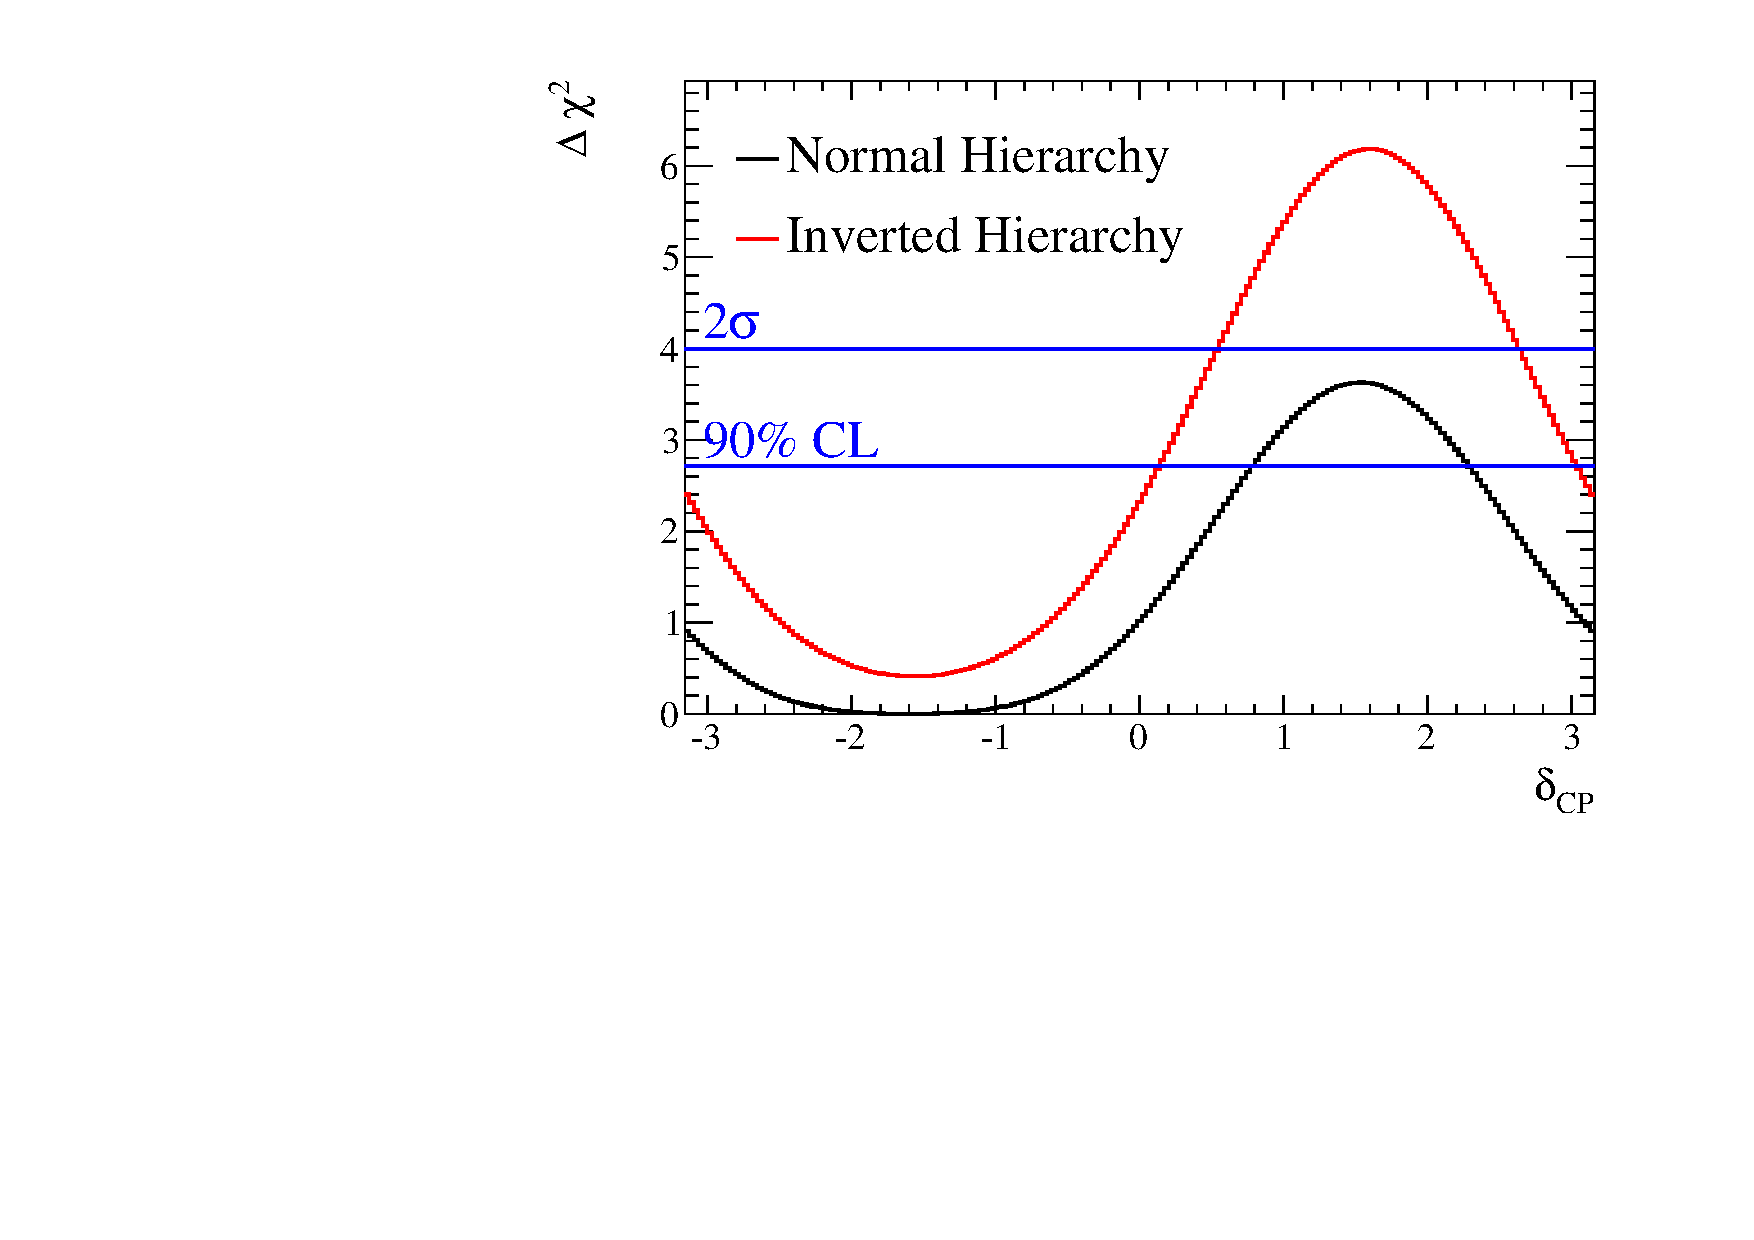
\includegraphics[width=0.9\textwidth]{./joint_plots/sensitivities/dcp_1D/dcp_react_Asimov_A.pdf}
\caption{Asimov A: with reactor constraint}
\end{subfigure}
\begin{subfigure}[b]{0.49\textwidth}
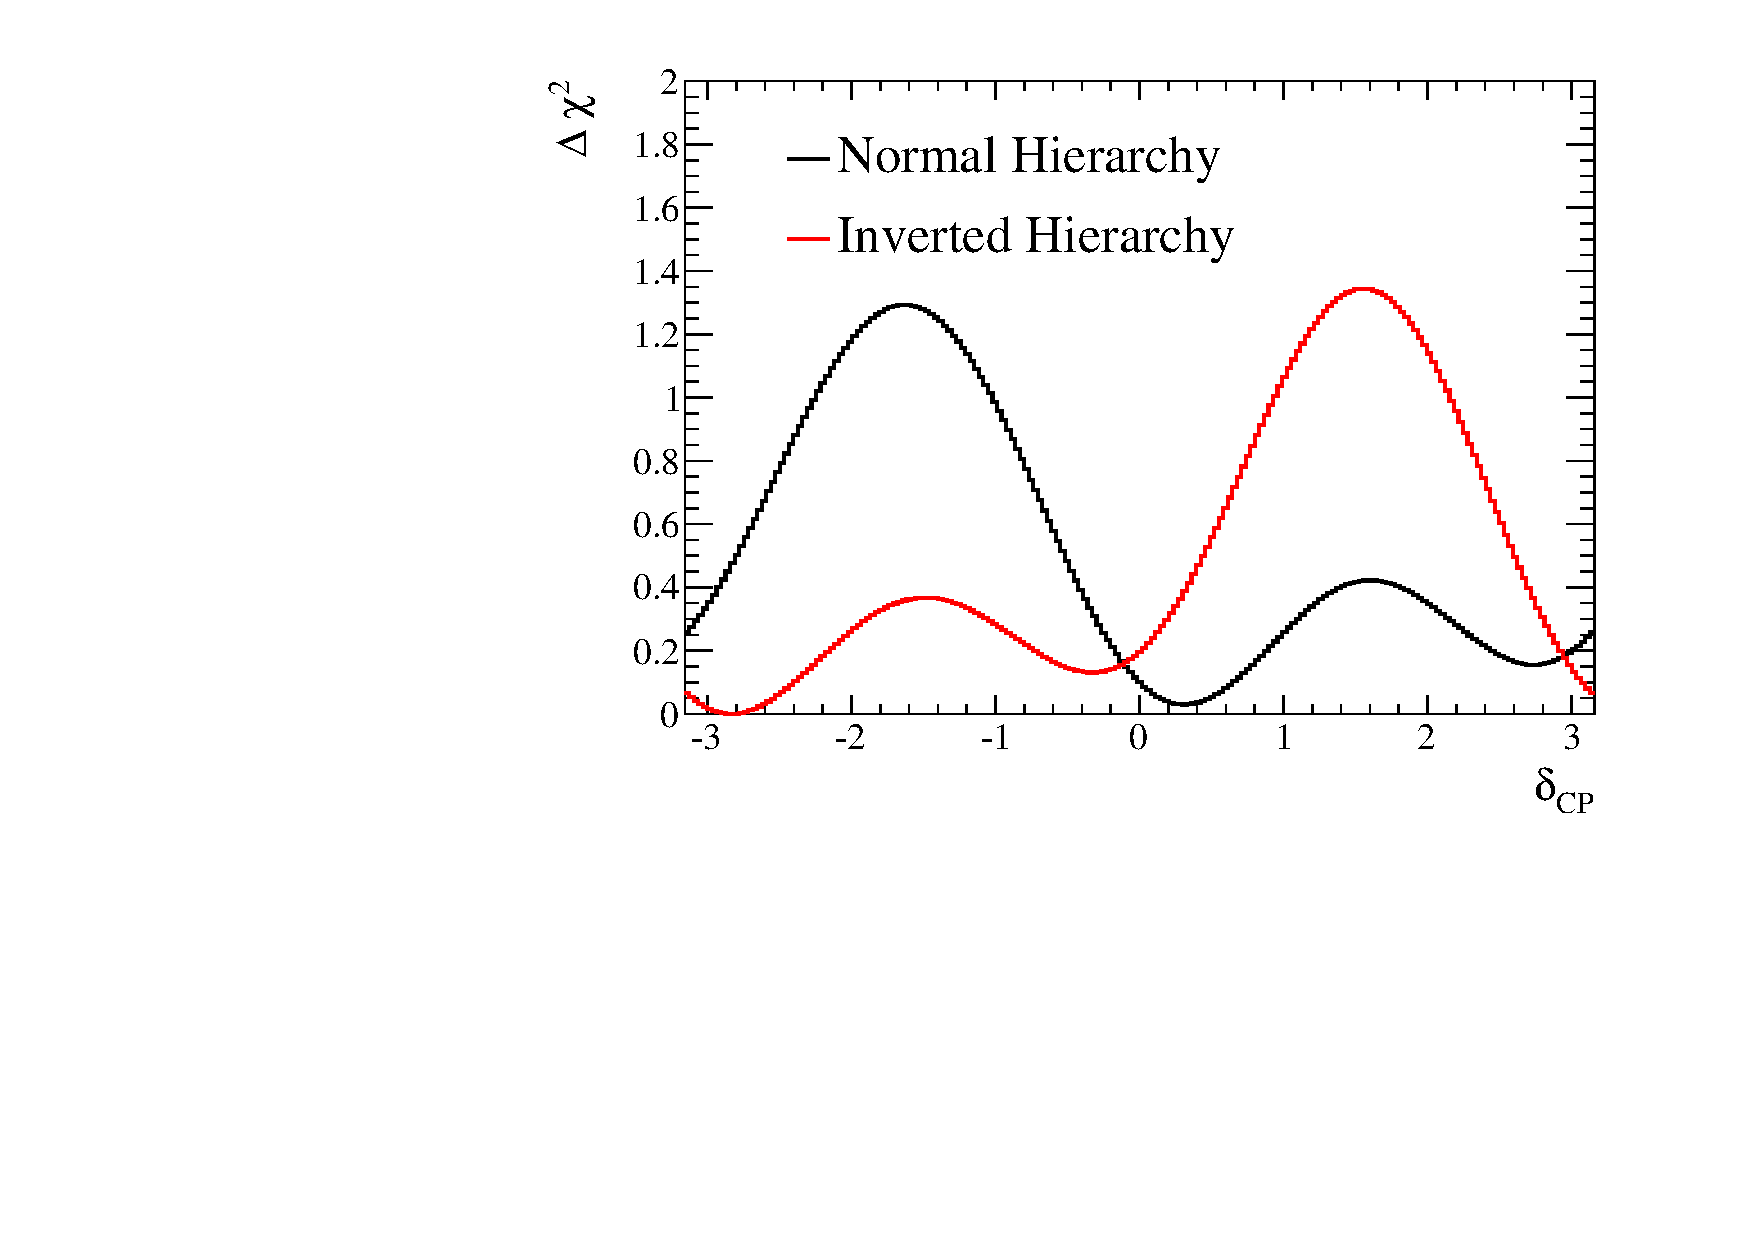
\includegraphics[width=0.9\textwidth]{./joint_plots/sensitivities/dcp_1D/dcp_react_Asimov_B.pdf} 
\caption{Asimov B: with reactor constraint}
\end{subfigure}
\begin{subfigure}[b]{0.49\textwidth}
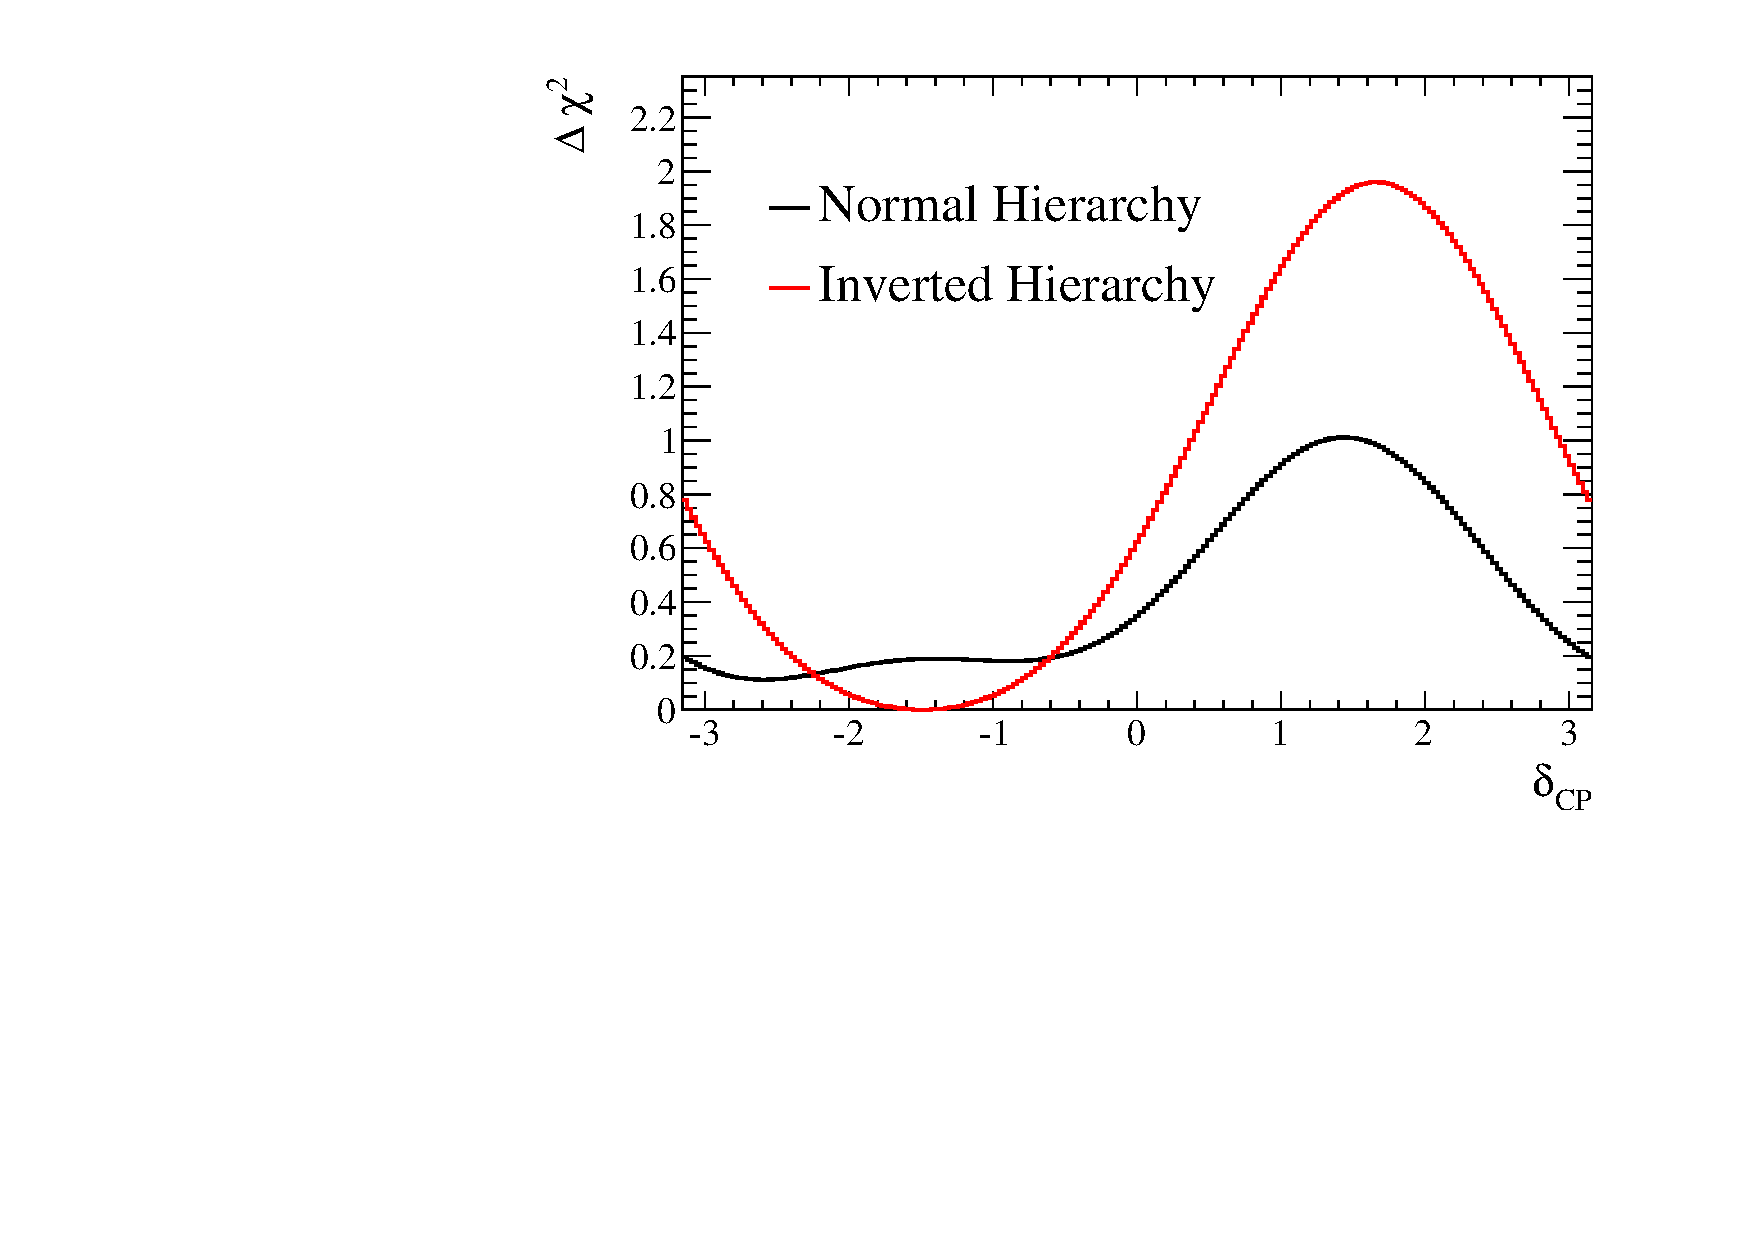
\includegraphics[width=0.9\textwidth]{./joint_plots/sensitivities/dcp_1D/dcp_t2konly_Asimov_A.pdf}
\caption{Asimov A: with T2K only}
\end{subfigure}
\begin{subfigure}[b]{0.49\textwidth}
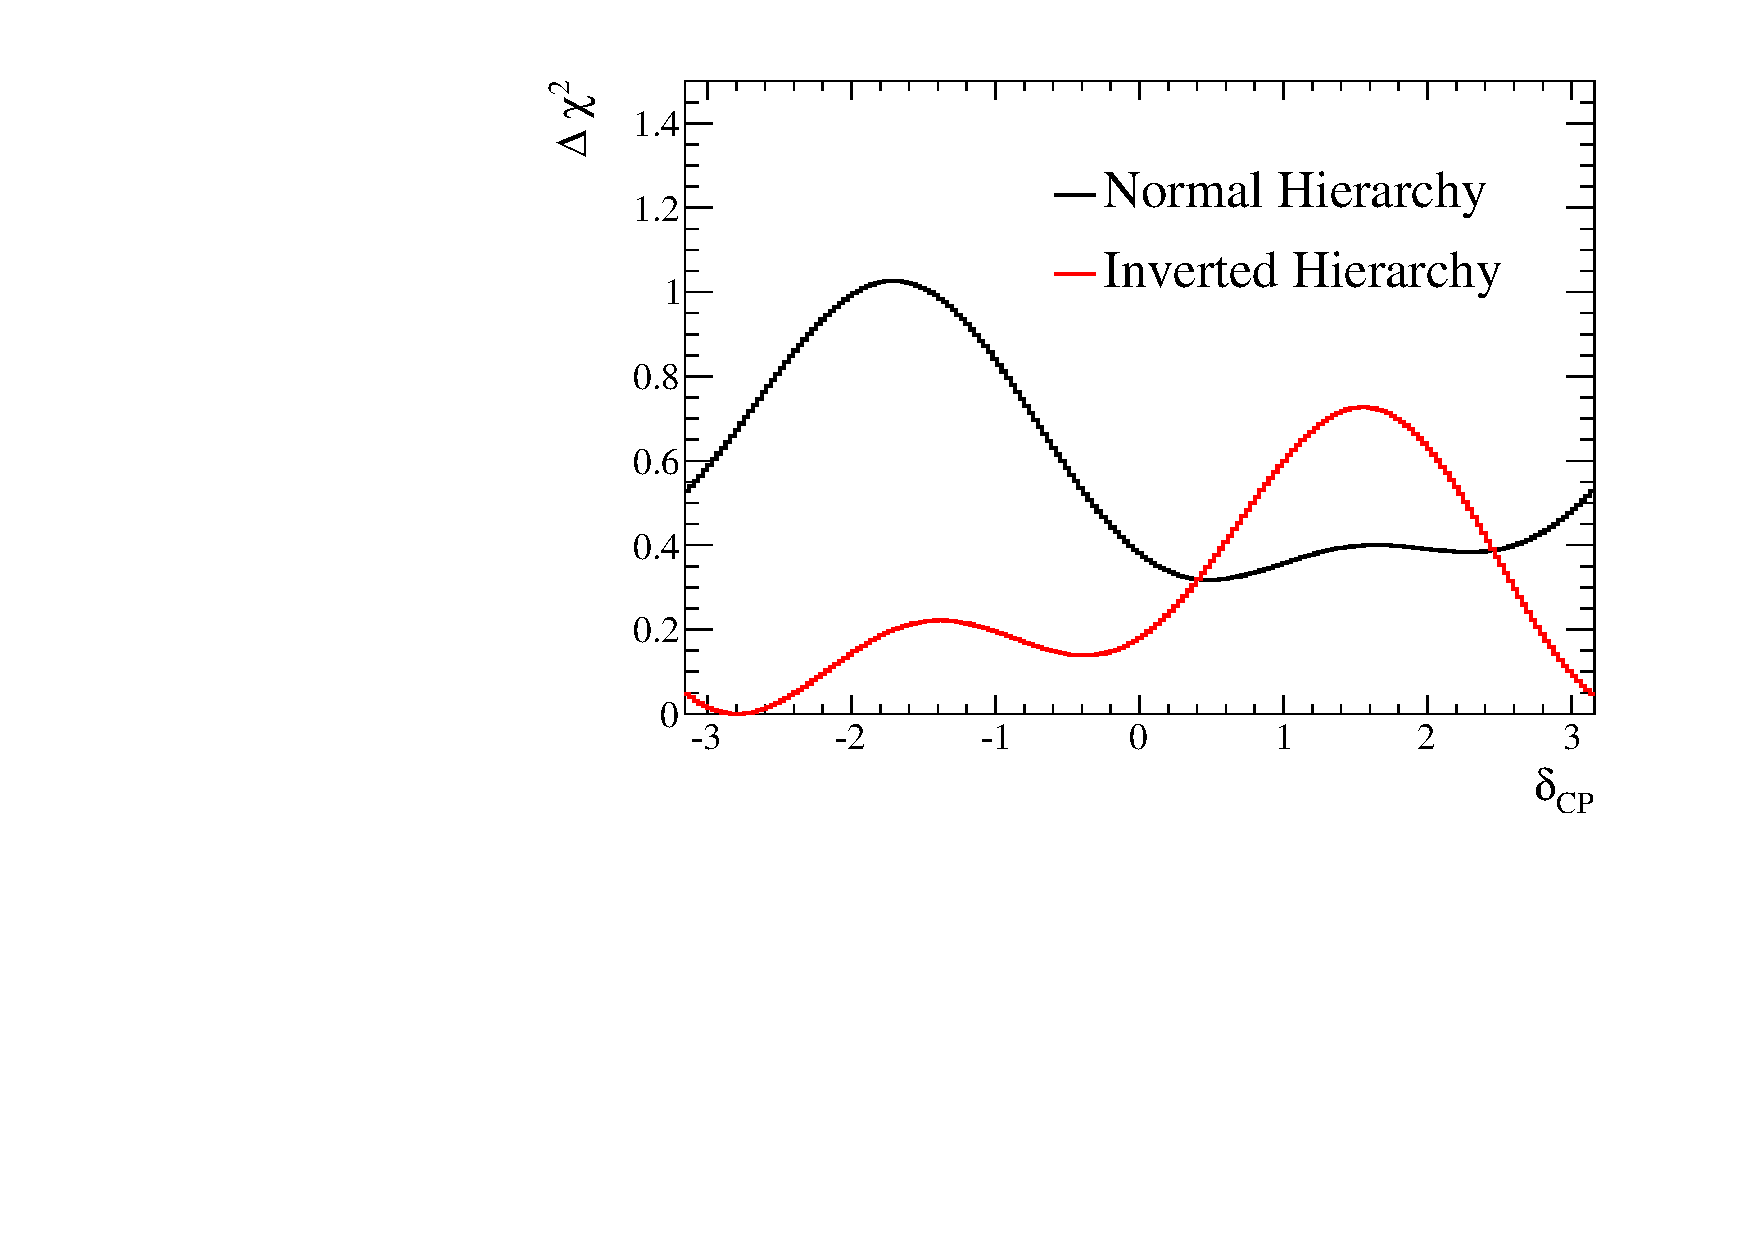
\includegraphics[width=0.9\textwidth]{./joint_plots/sensitivities/dcp_1D/dcp_t2konly_Asimov_B.pdf}
\caption{Asimov B: with T2K only}
\end{subfigure}
\caption {
%{\large{SENSI DELTACHISQ 1D DELTACP W/ AND W/O REACTORS}}
The expected $\Delta \chi^2$ distribution as a function of $\delta_{CP}$ 
for the Asimov data sets A and B of Tab.~\ref{tab:osc_params_joint_asimov} 
corresponding to the Run 1-6 statistics
is compared to the result obtained by the other analysis groups.
The mass hierarchy is minimized:
both the normal and inverted hierarchy $\chi^2$ distributions 
are shifted to the same global best-fit $\chi^2$ value,
which is taken as the minimum between normal and inverted hierarchy.
}
\label{fig:validation_sensi_dcp}
\end{figure*}

Also the sensitivity to $\sin^2 \theta_{13}$ Vs $\delta_{CP}$ 
with reactor constraint and T2K only data,
and $\sin^2 \theta_{23}$ Vs $m^2_{32}$ ($m^2_{13}$) with reactor constraint 
%compared to the ones of the other analyses groups,
are shown in Fig.~\ref{fig:validation_sensi_2d_reactors} 
and 
\ref{fig:validation_sensi_2d_t2konly},
where normal and inverted hierarchy contours are set independently,
i.e. each calculated with respect to its own minimum $\chi^2$ value
and not the global minimum as a function of the mass hierarchy.

\begin{figure*}[htb]
\center
%
\includegraphics[width=0.9\textwidth]{./images/missing_plot-eps-converted-to.pdf}
%
\includegraphics[width=0.9\textwidth]{./images/missing_plot-eps-converted-to.pdf}
%
\includegraphics[width=0.9\textwidth]{./images/missing_plot-eps-converted-to.pdf}
%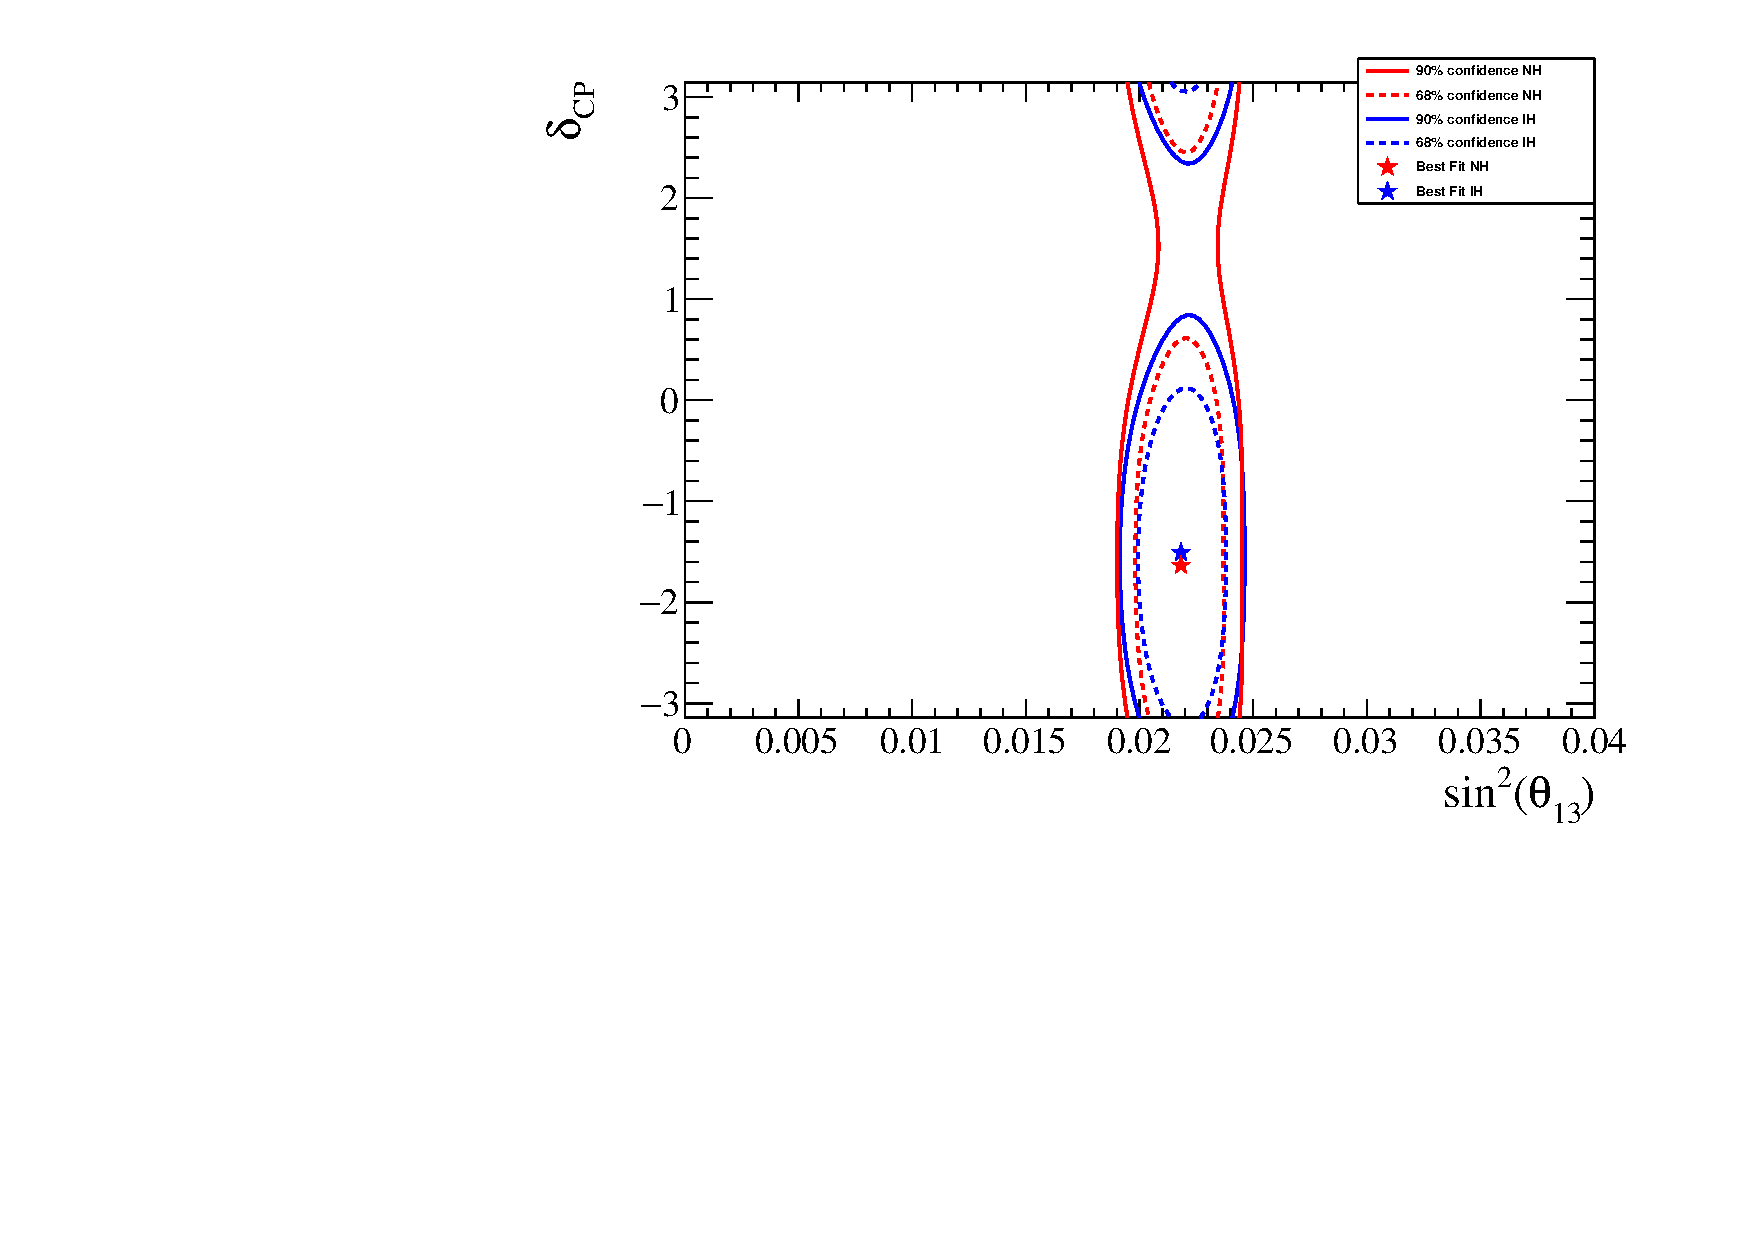
\includegraphics[width=0.9\textwidth]{./joint_plots/sensitivities/2D/cp13_reactor/cp13_reactor_A.pdf}
%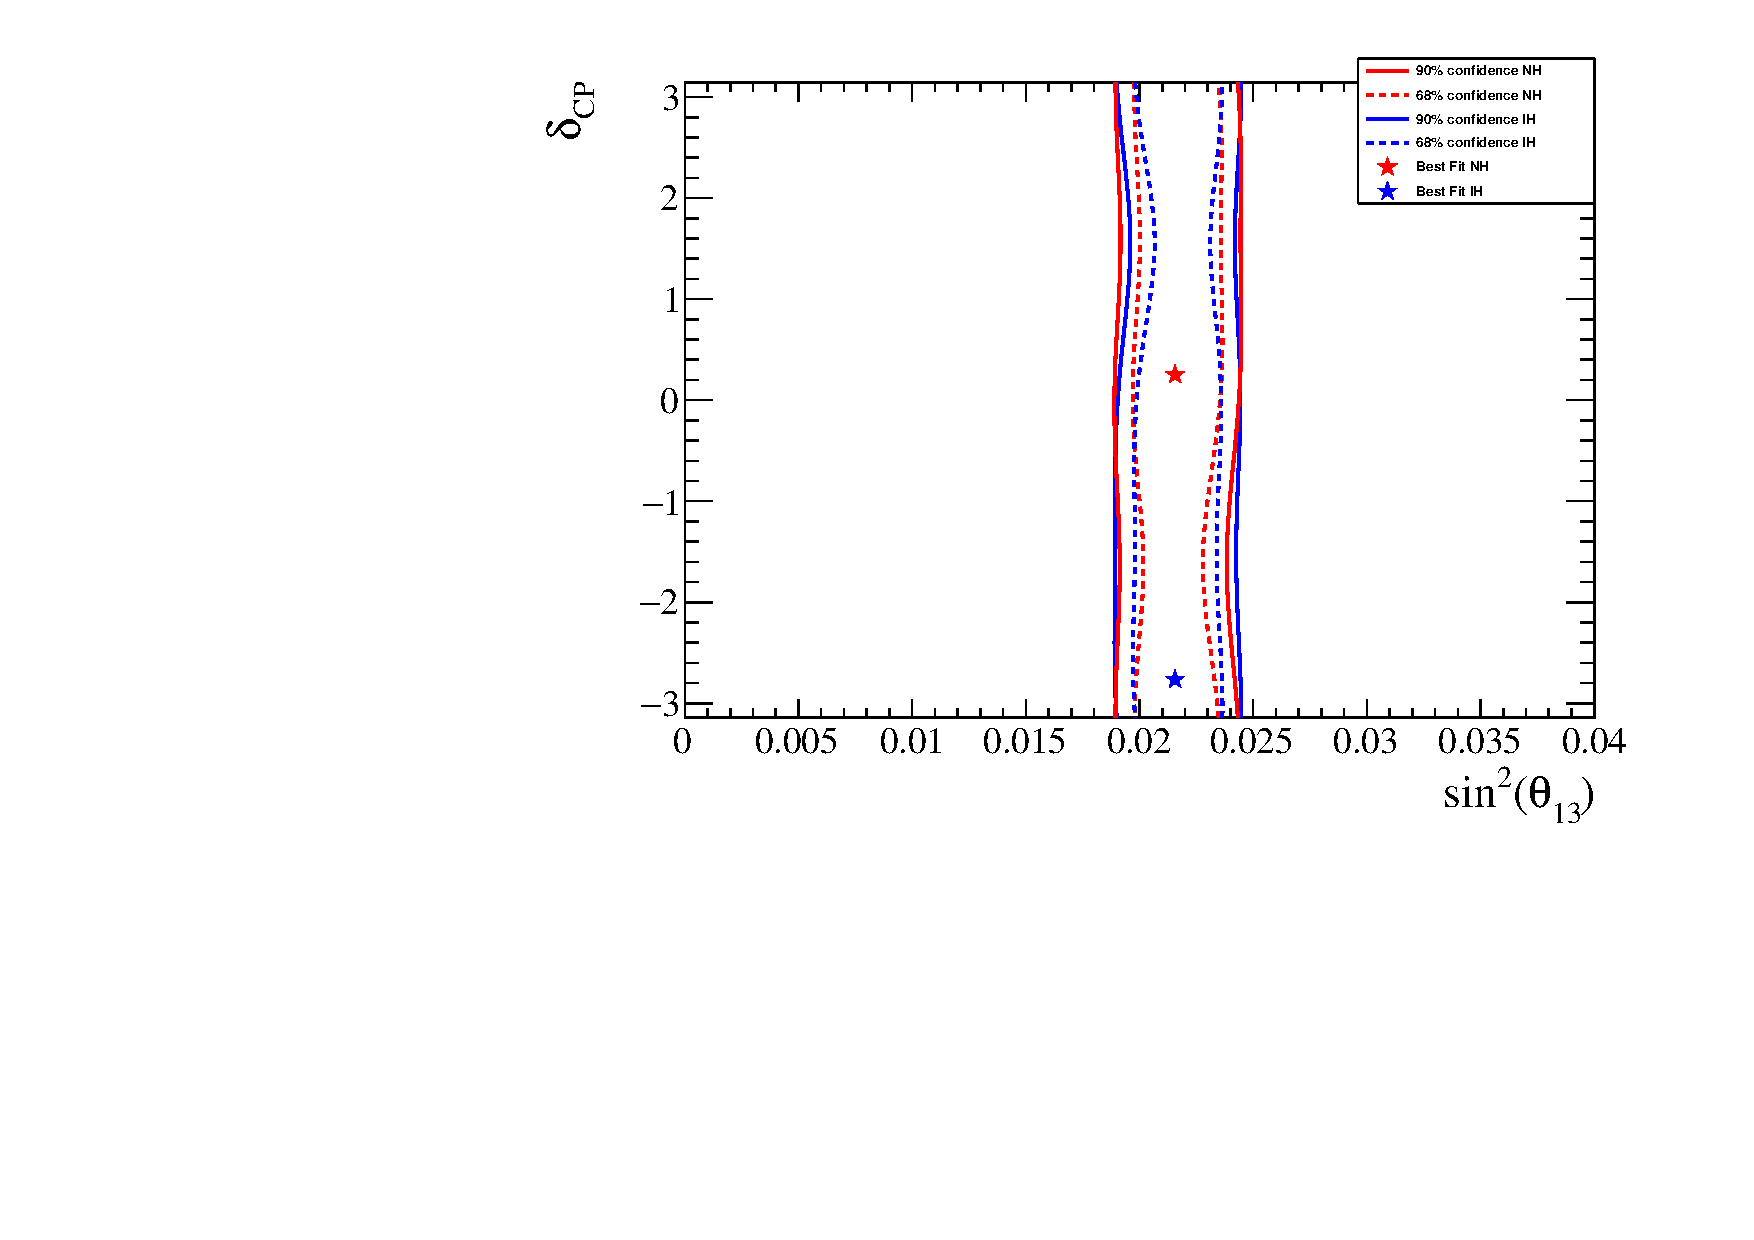
\includegraphics[width=0.9\textwidth]{./joint_plots/sensitivities/2D/cp13_reactor/cp13_reactor_B.pdf}
%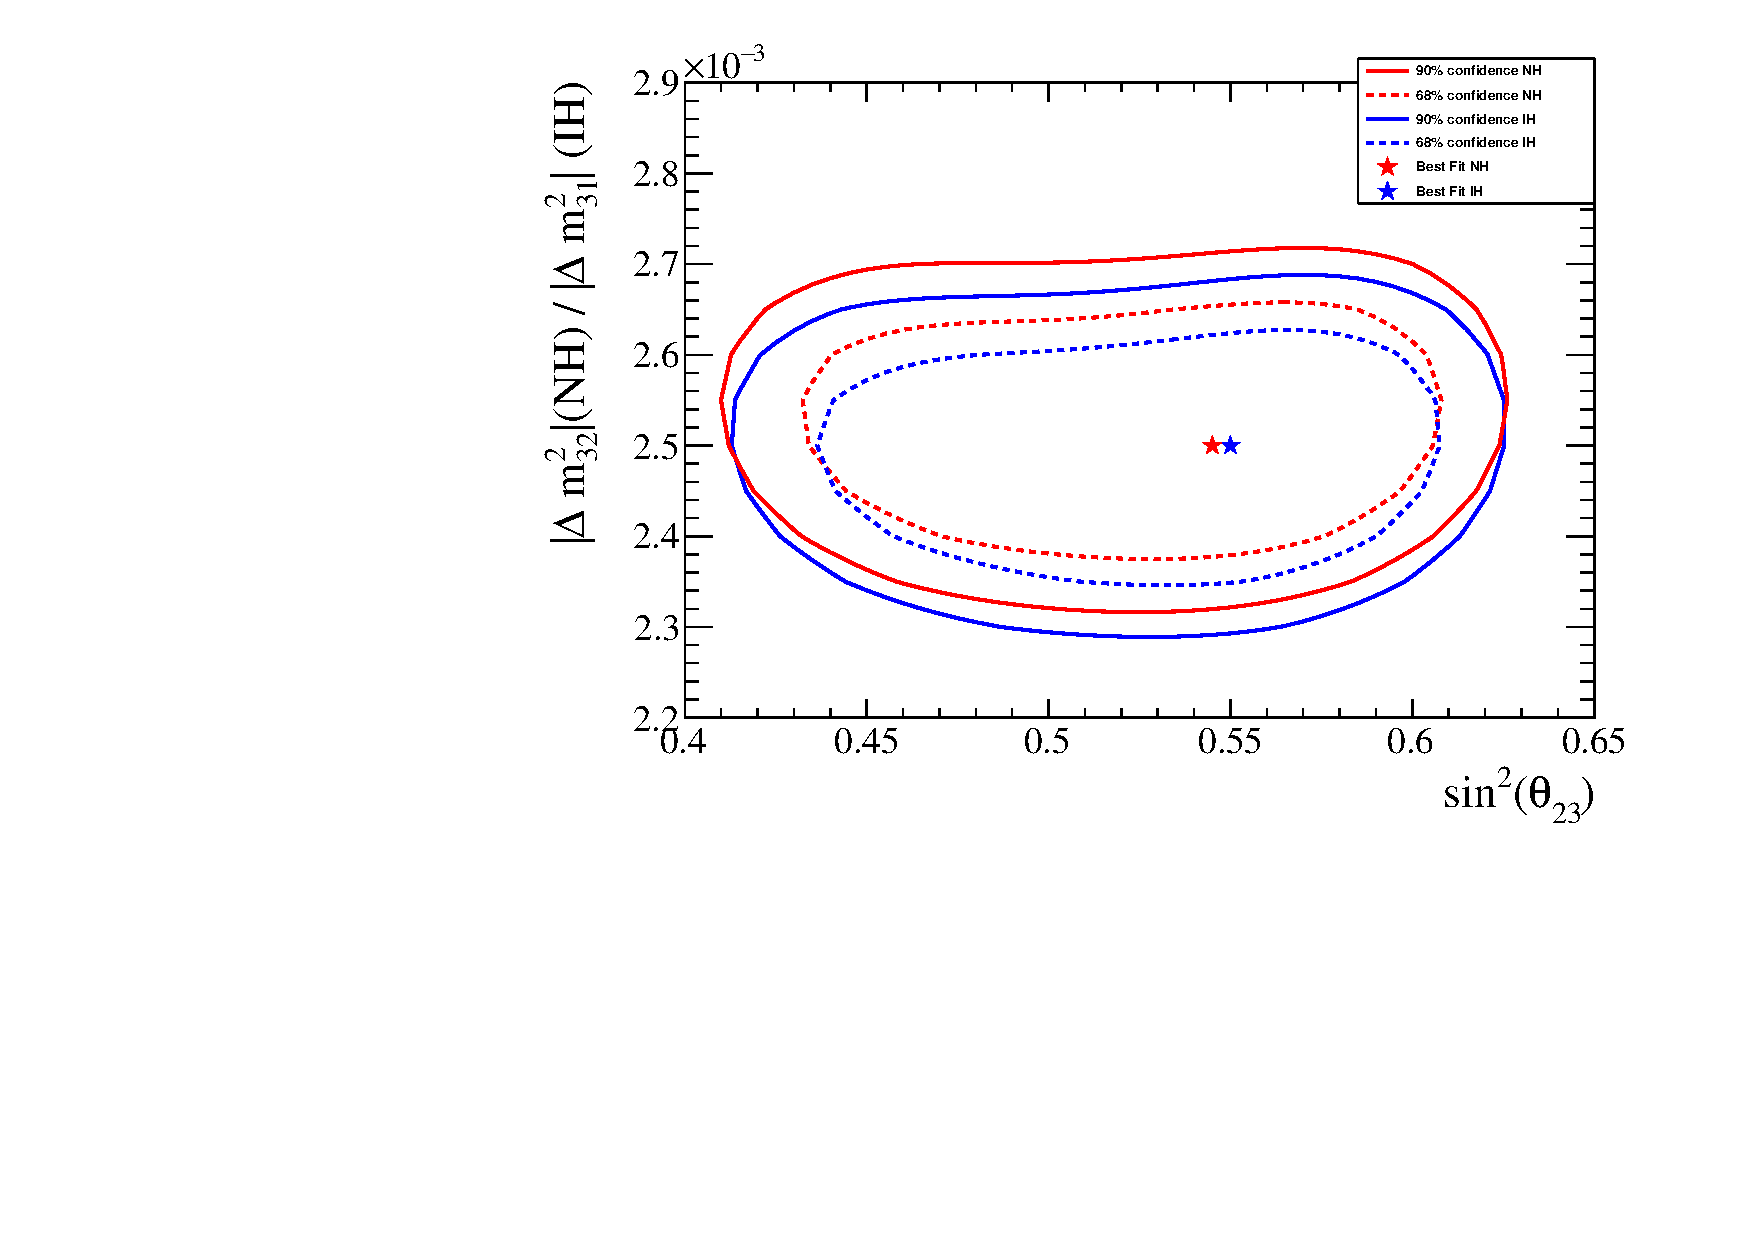
\includegraphics[width=0.9\textwidth]{./joint_plots/sensitivities/2D/ss23dmsq/ss23dmsq_A.pdf}
%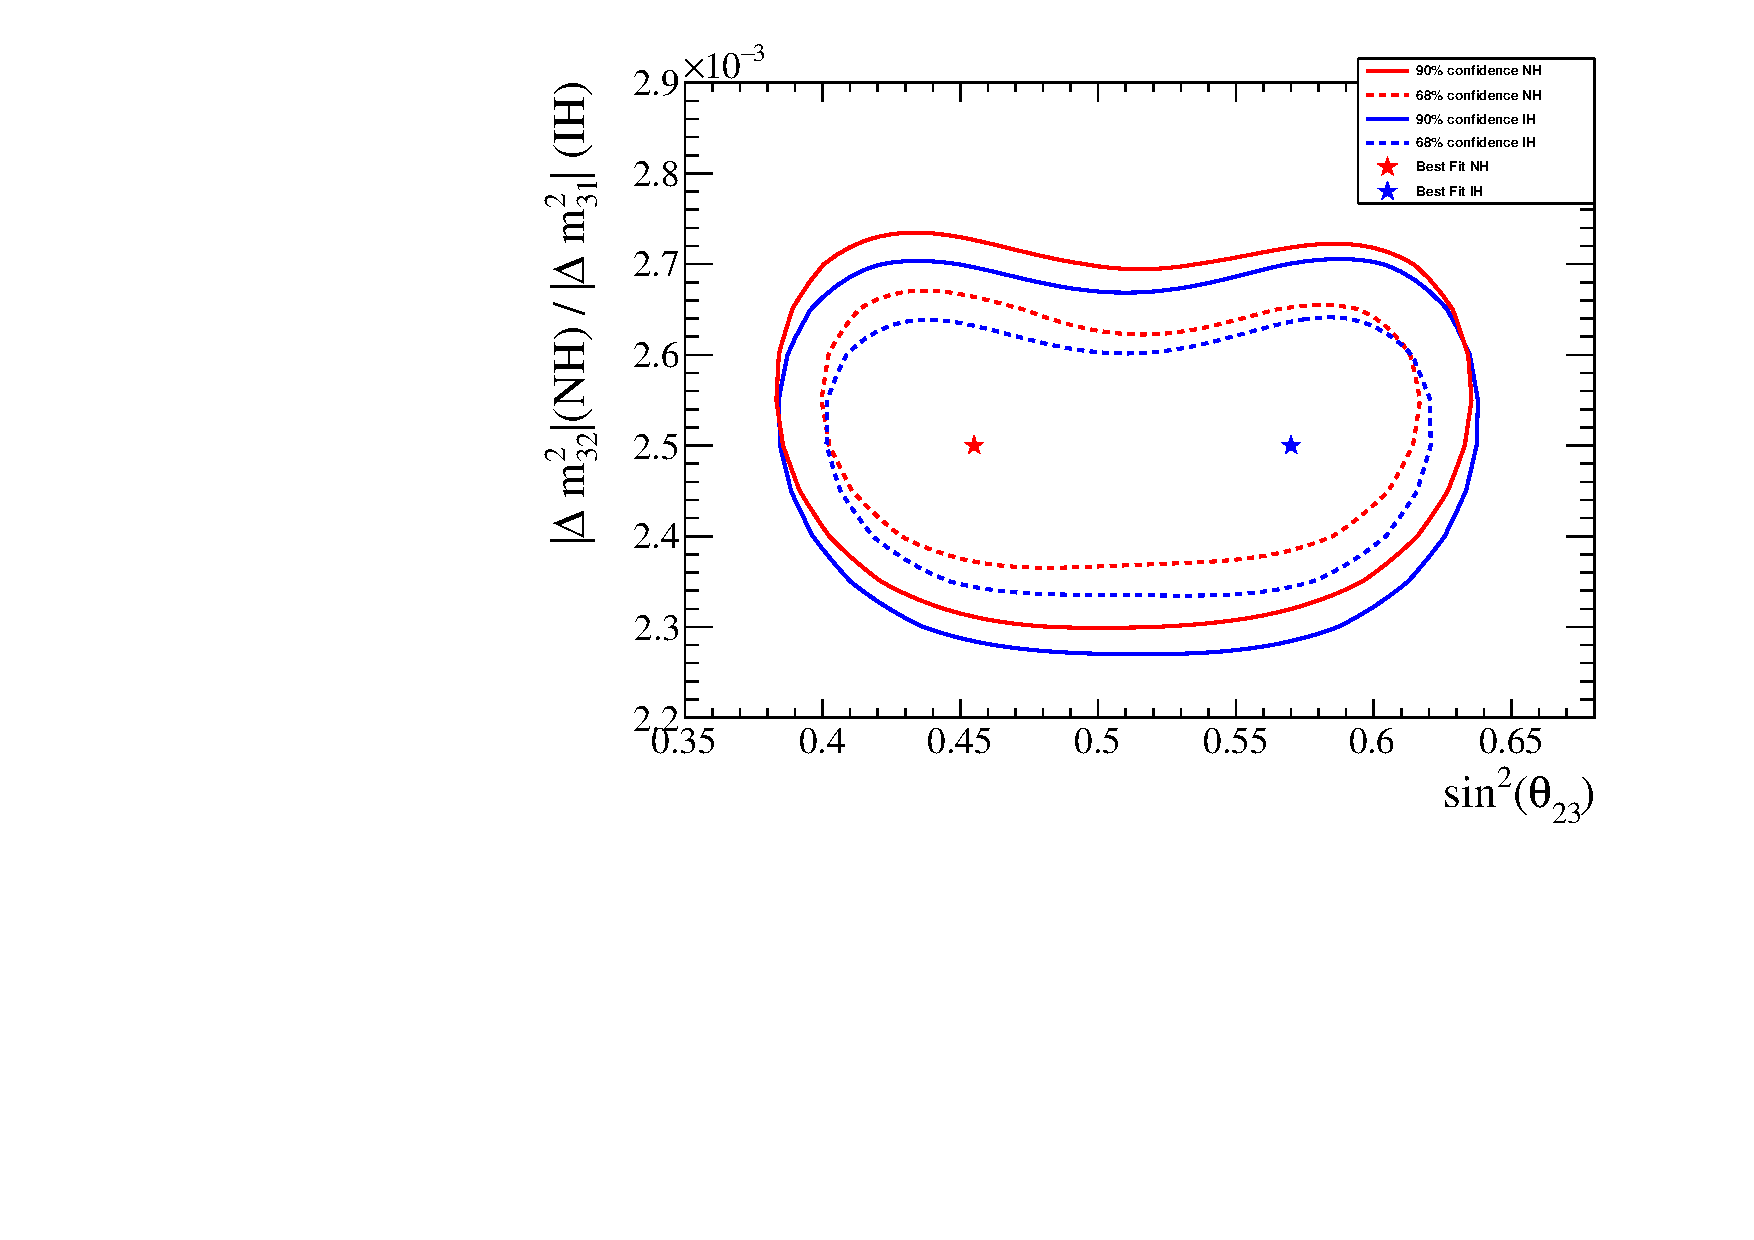
\includegraphics[width=0.9\textwidth]{./joint_plots/sensitivities/2D/ss23dmsq/ss23dmsq_B.pdf}
\begin{subfigure}[b]{0.49\textwidth}
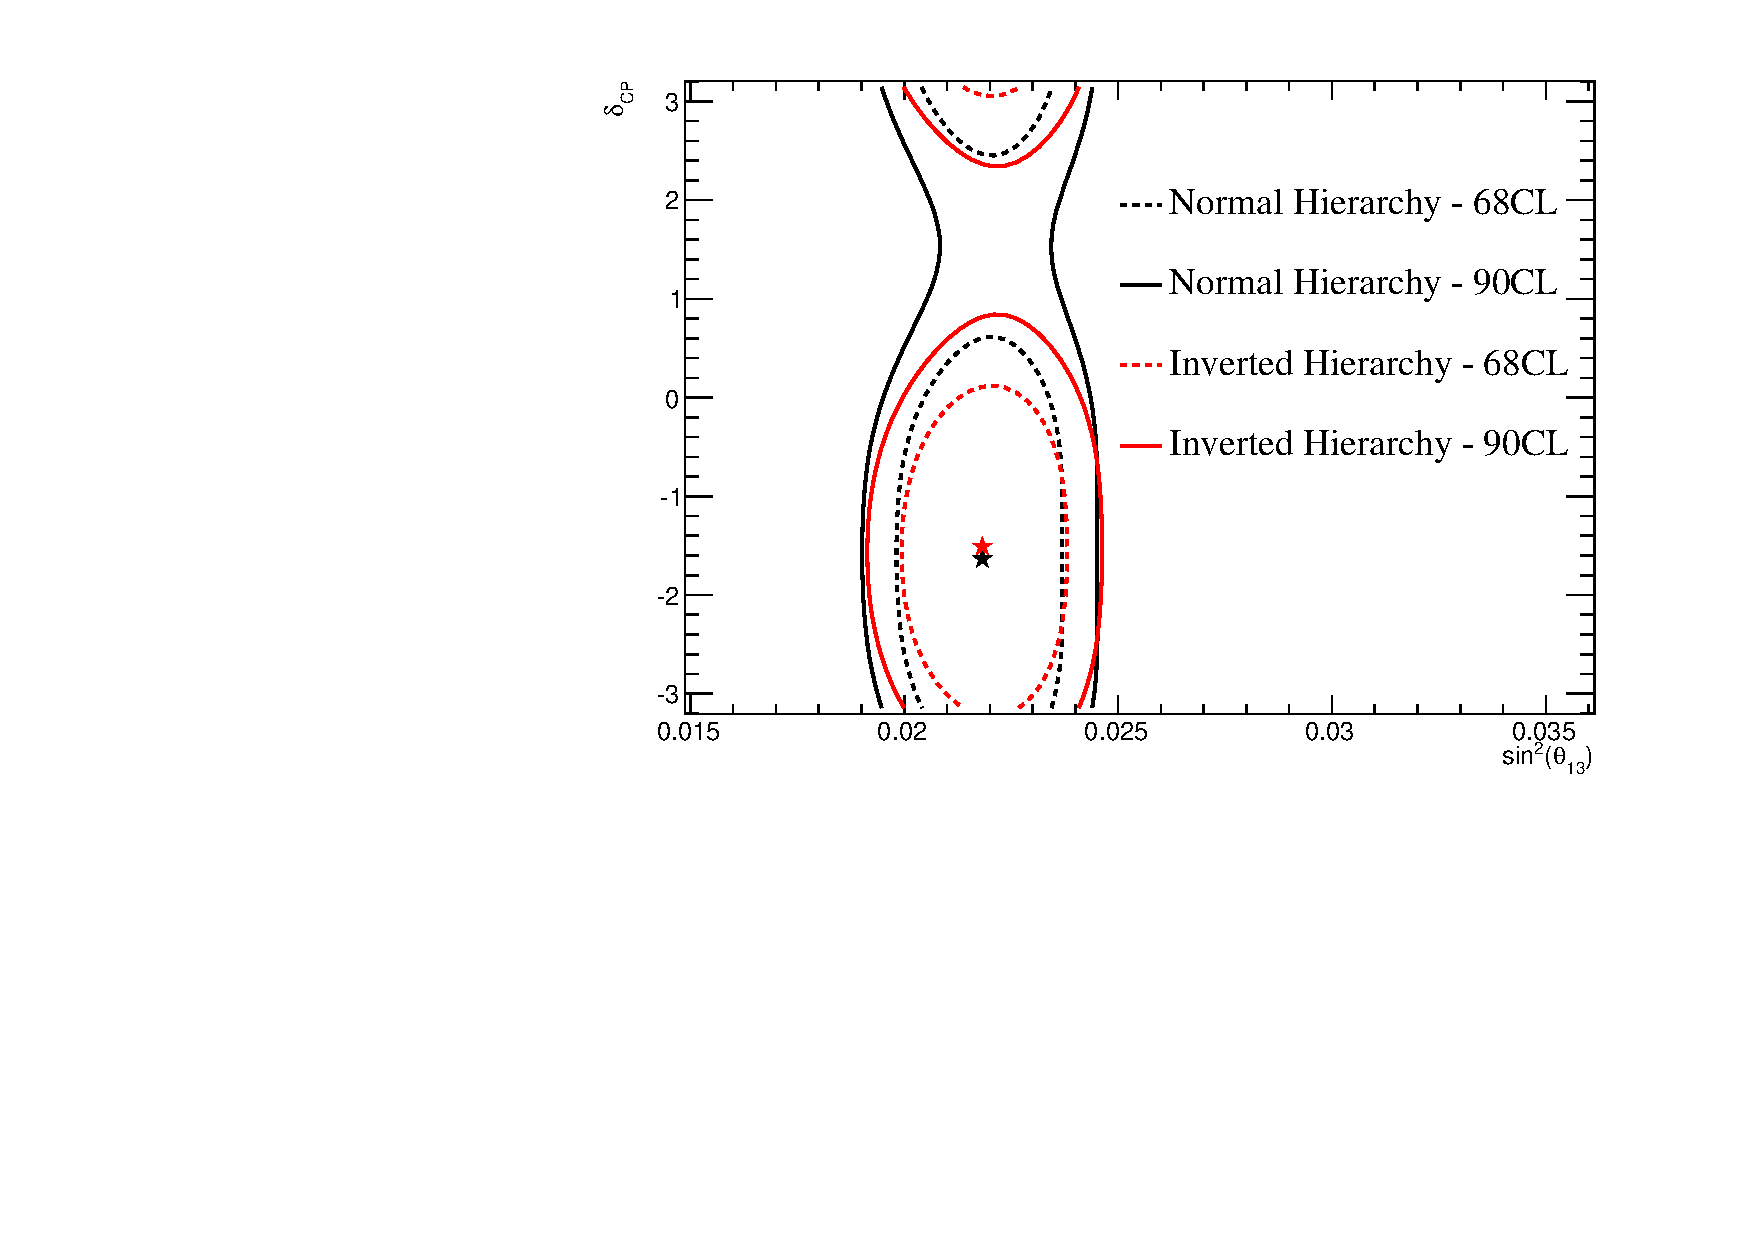
\includegraphics[width=0.9\textwidth]{./joint_plots/sensitivities/2D/contour_joint_sinsqth13Vsdcp_Asimov_A_react}
\caption{Asimov A: $\sin^2 \theta_{13}$ Vs $\delta_{CP}$}
\end{subfigure}
\begin{subfigure}[b]{0.49\textwidth}
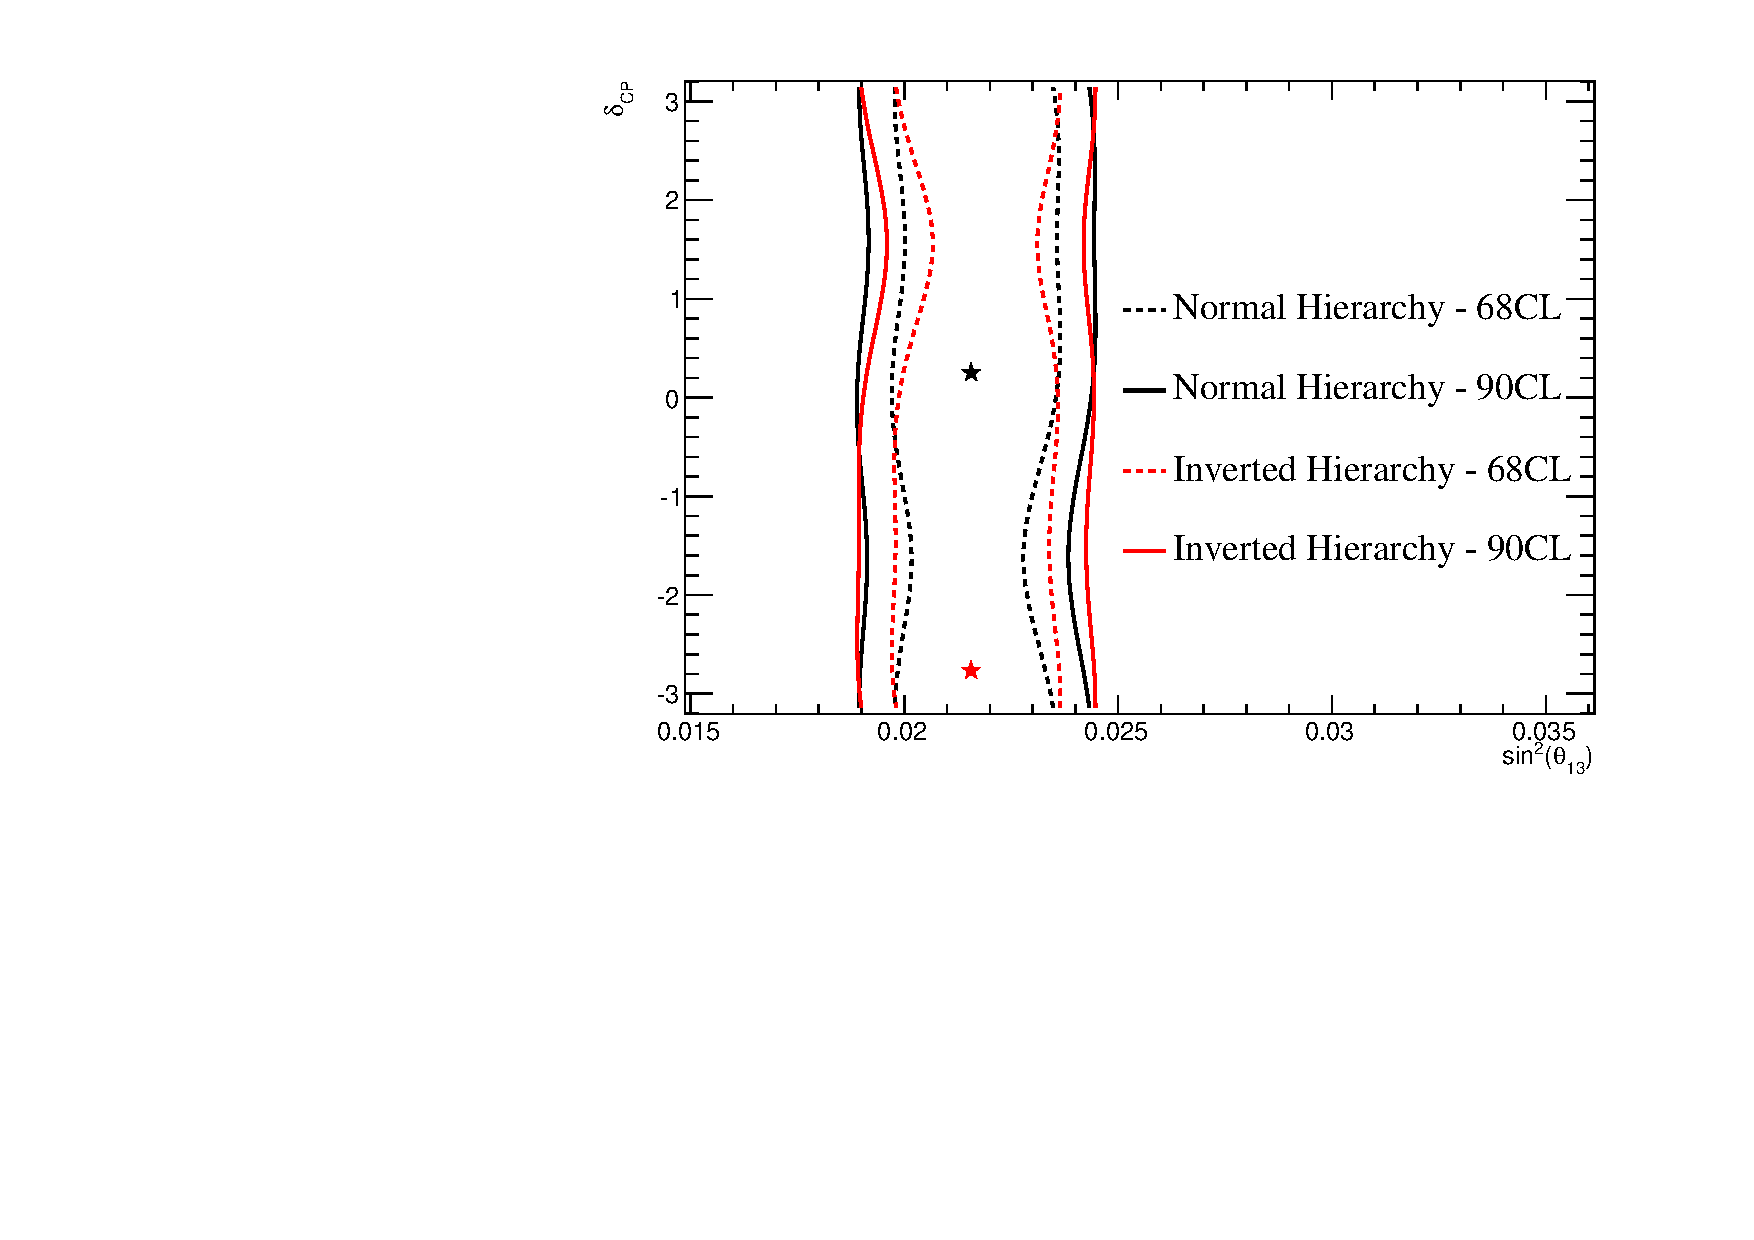
\includegraphics[width=0.9\textwidth]{./joint_plots/sensitivities/2D/contour_joint_sinsqth13Vsdcp_Asimov_B_react} 
\caption{Asimov B: $\sin^2 \theta_{13}$ Vs $\delta_{CP}$}
\end{subfigure}
\begin{subfigure}[b]{0.49\textwidth}
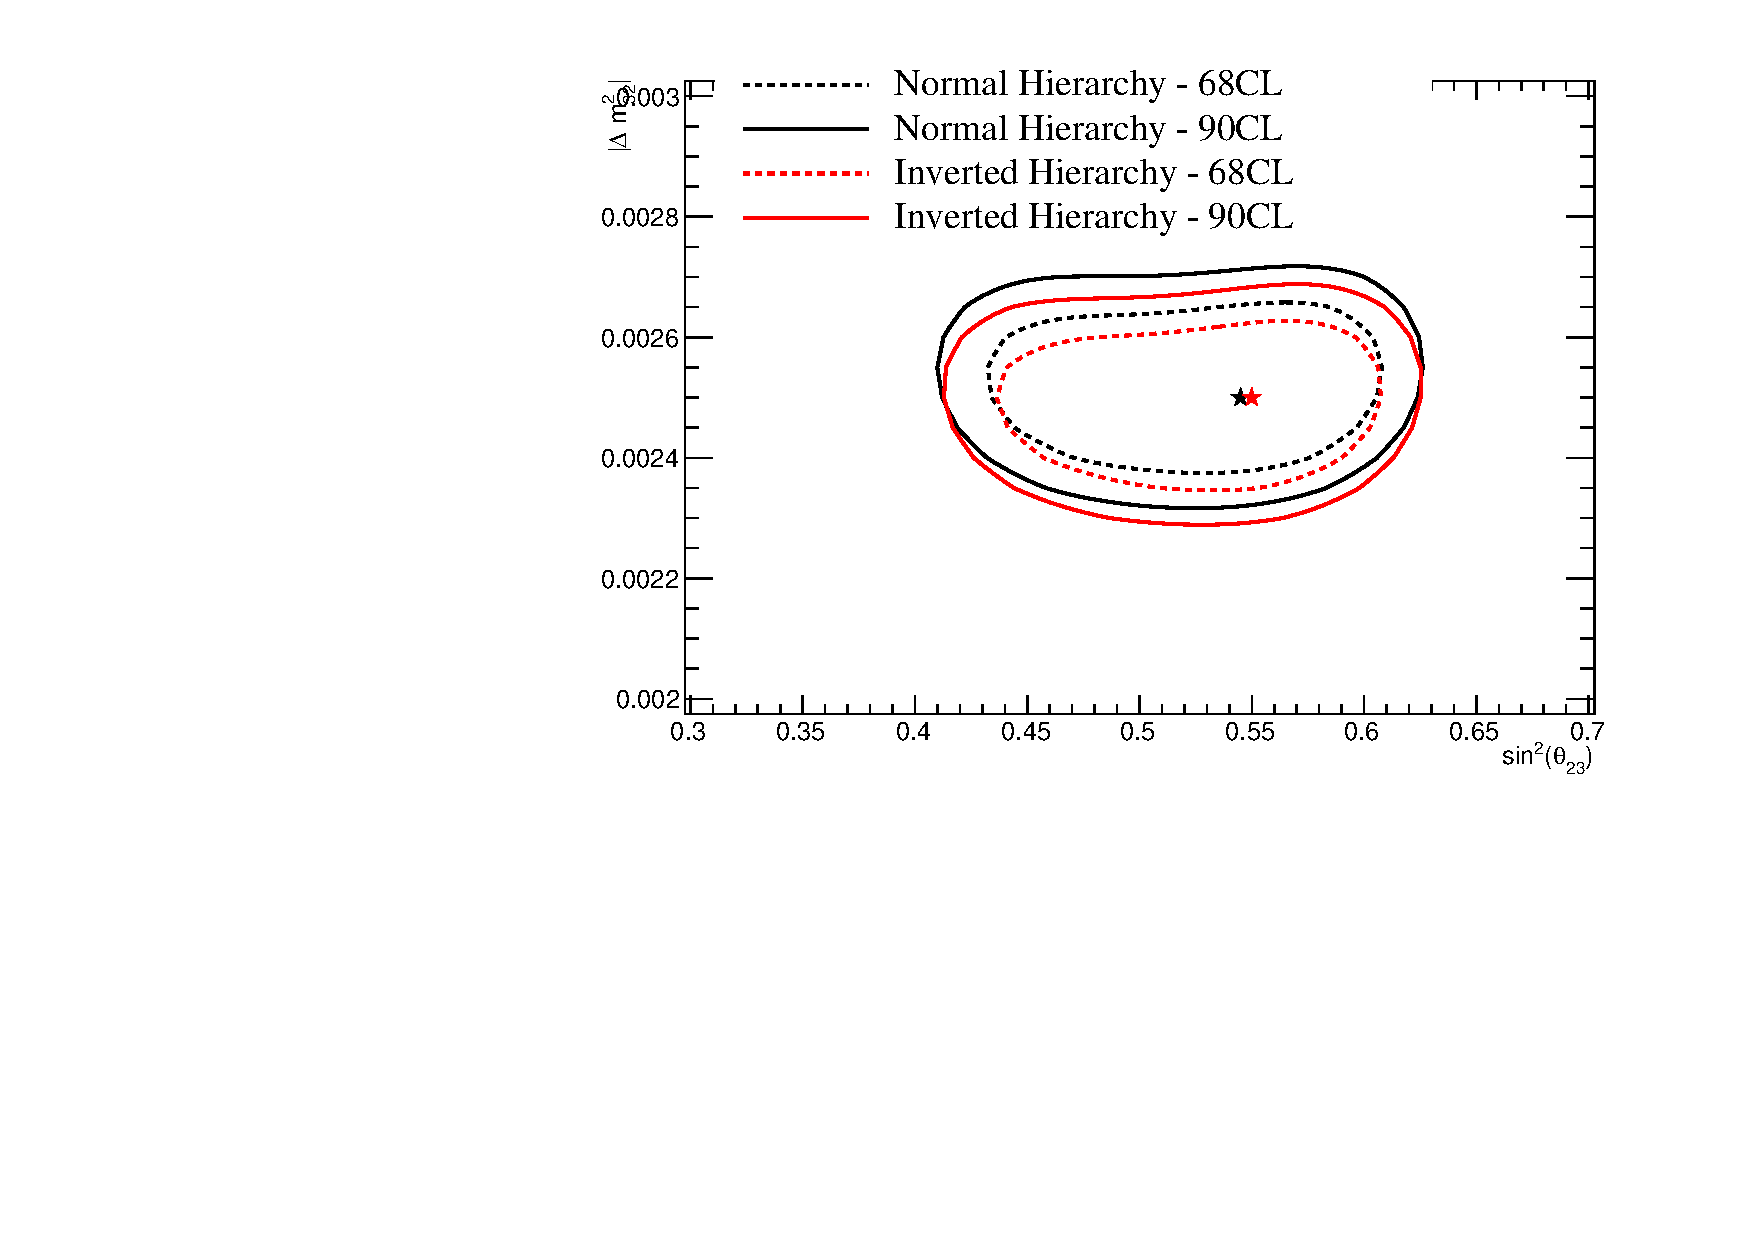
\includegraphics[width=0.9\textwidth]{./joint_plots/sensitivities/2D/contour_joint_sinsqth23Vsdmsq_Asimov_A_react}
\caption{Asimov A: $\sin^2 \theta_{23}$ Vs $\Delta m^2_{32}$ ($m^2_{13}$)}
\end{subfigure}
\begin{subfigure}[b]{0.49\textwidth}
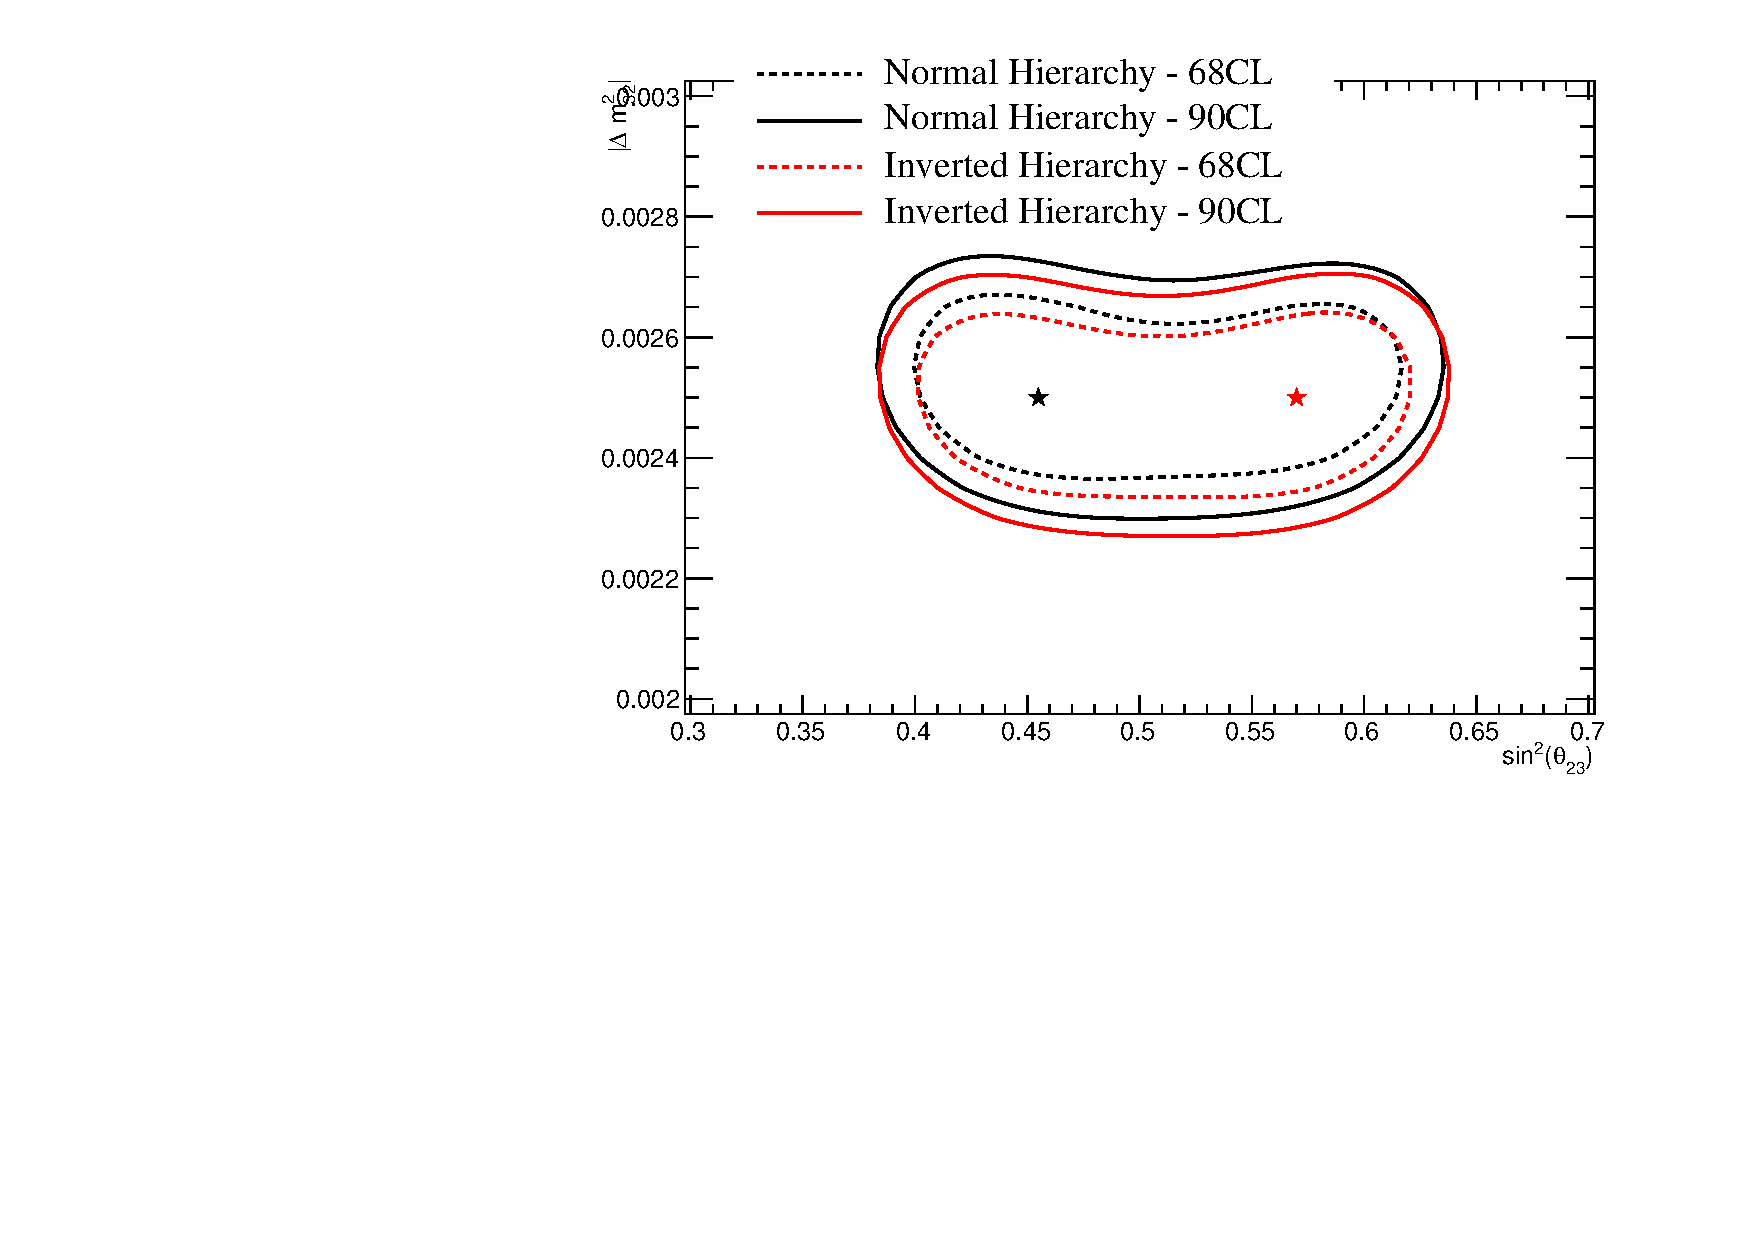
\includegraphics[width=0.9\textwidth]{./joint_plots/sensitivities/2D/contour_joint_sinsqth23Vsdmsq_Asimov_B_react}
\caption{Asimov B: $\sin^2 \theta_{23}$ Vs $\Delta m^2_{32}$ ($m^2_{13}$)}
\end{subfigure}
\caption {
%{\large{SENSI 2D CONTOURS W/ AND W/O REACTORS}}
The contours at 68\% and 90\% CL with reactor constraint 
for the Asimov data sets A and B of tab.~\ref{tab:osc_params_joint_asimov} 
corresponding to the Run 1-6 statistics 
is shown.
%is compared to the result obtained by the other analysis groups.
Normal and inverted hierarchy contours are independent.
}
\label{fig:validation_sensi_2d_reactors}
\end{figure*}

\begin{figure*}[htb]
\center
\begin{subfigure}[b]{0.49\textwidth}
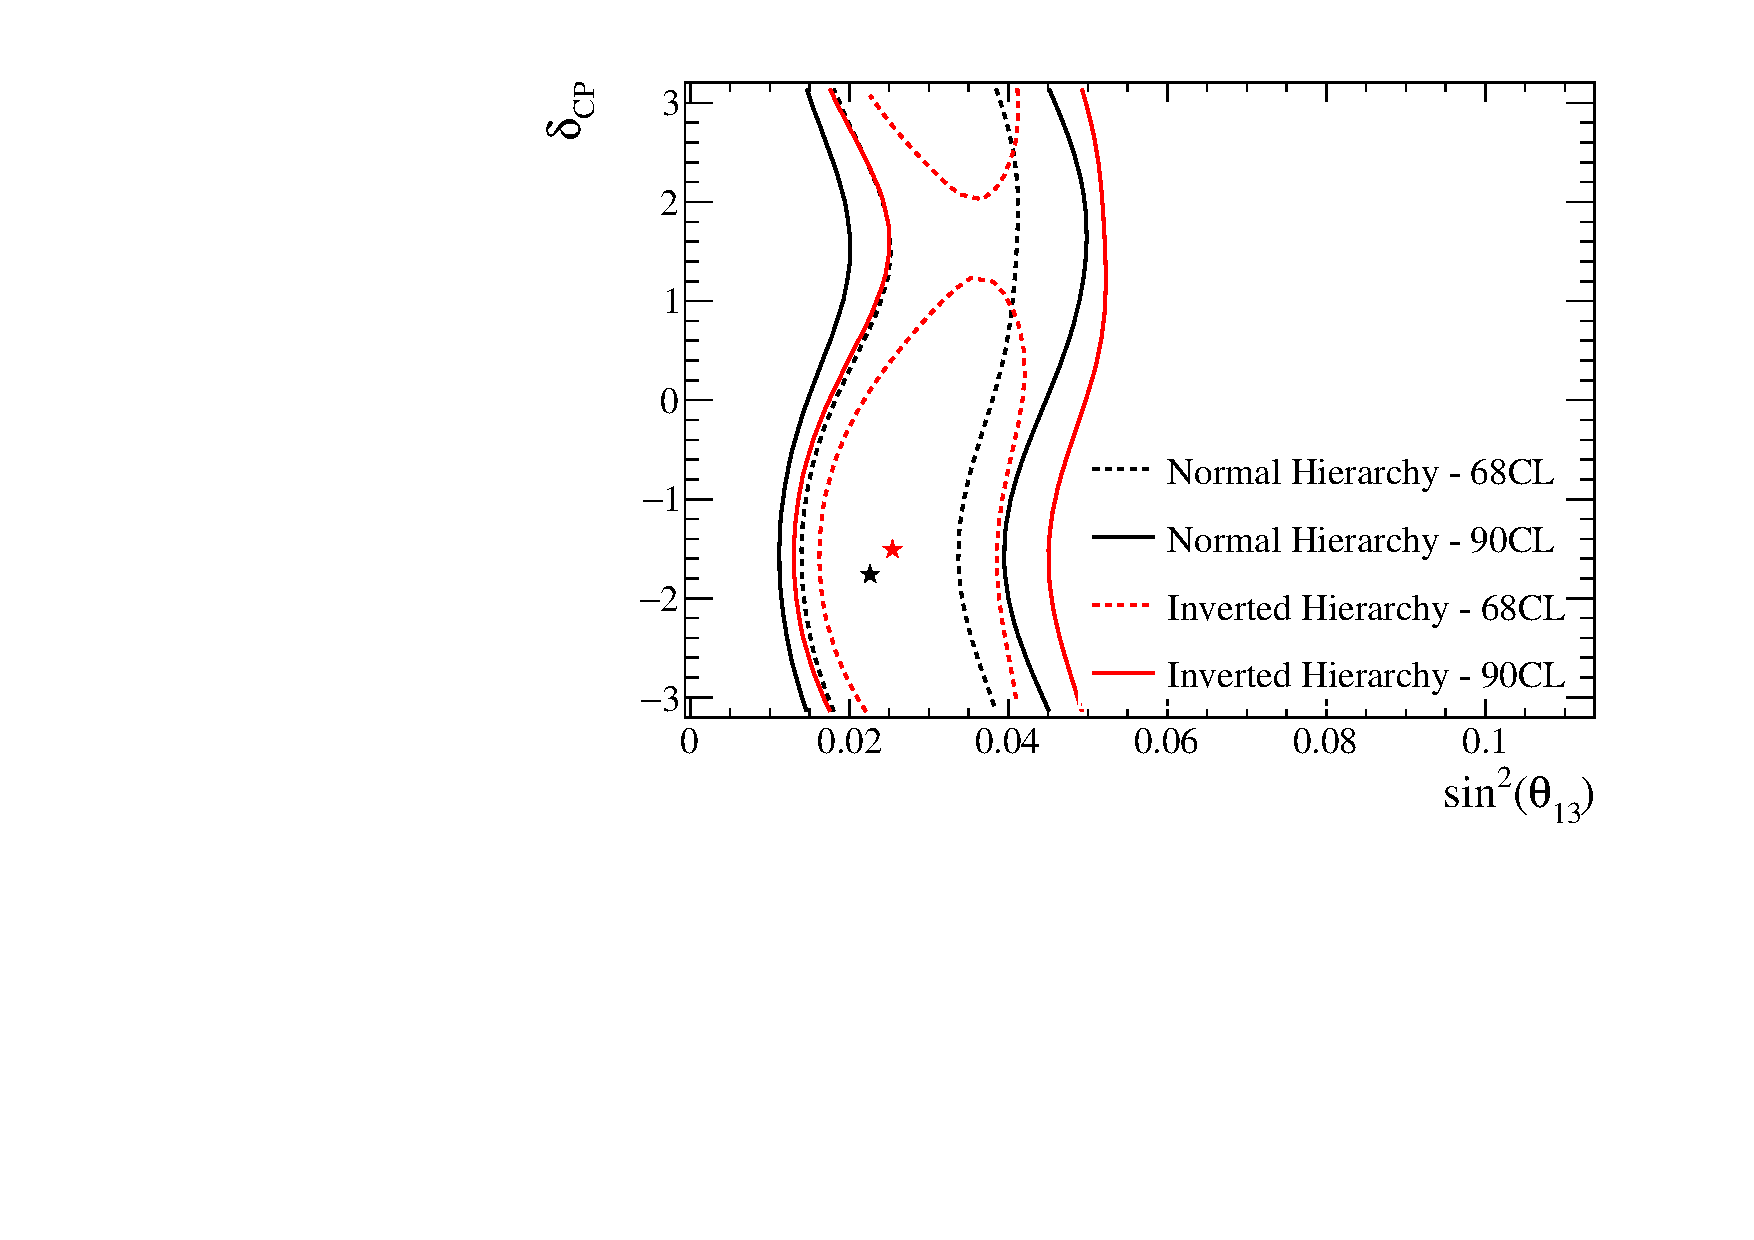
\includegraphics[width=0.9\textwidth]{./joint_plots/sensitivities/2D/cp13/cp13_A.pdf}
\caption{Asimov A with reactor constraint}
\end{subfigure}
\begin{subfigure}[b]{0.49\textwidth}
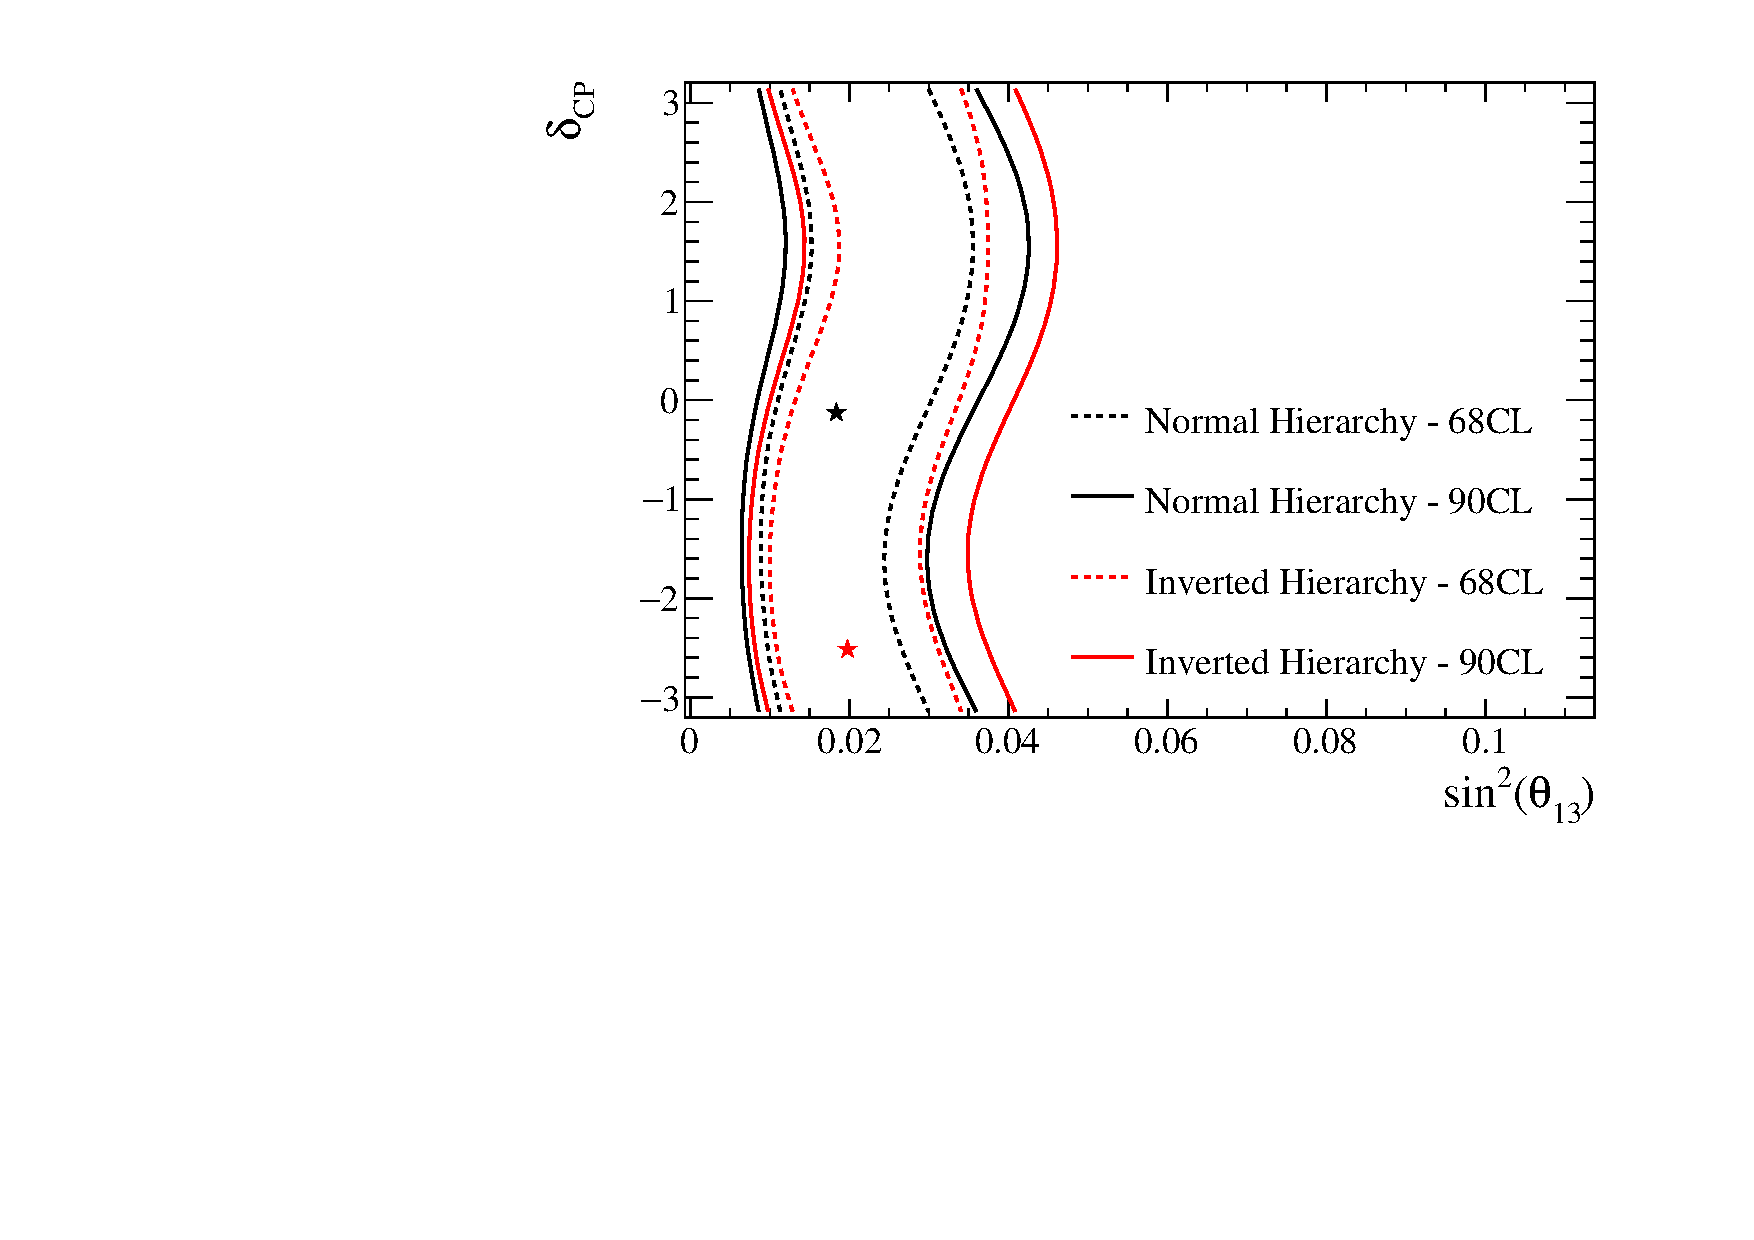
\includegraphics[width=0.9\textwidth]{./joint_plots/sensitivities/2D/cp13/cp13_B.pdf}
\caption{Asimov B with reactor constraint}
\end{subfigure}

%\begin{subfigure}[b]{0.49\textwidth}
%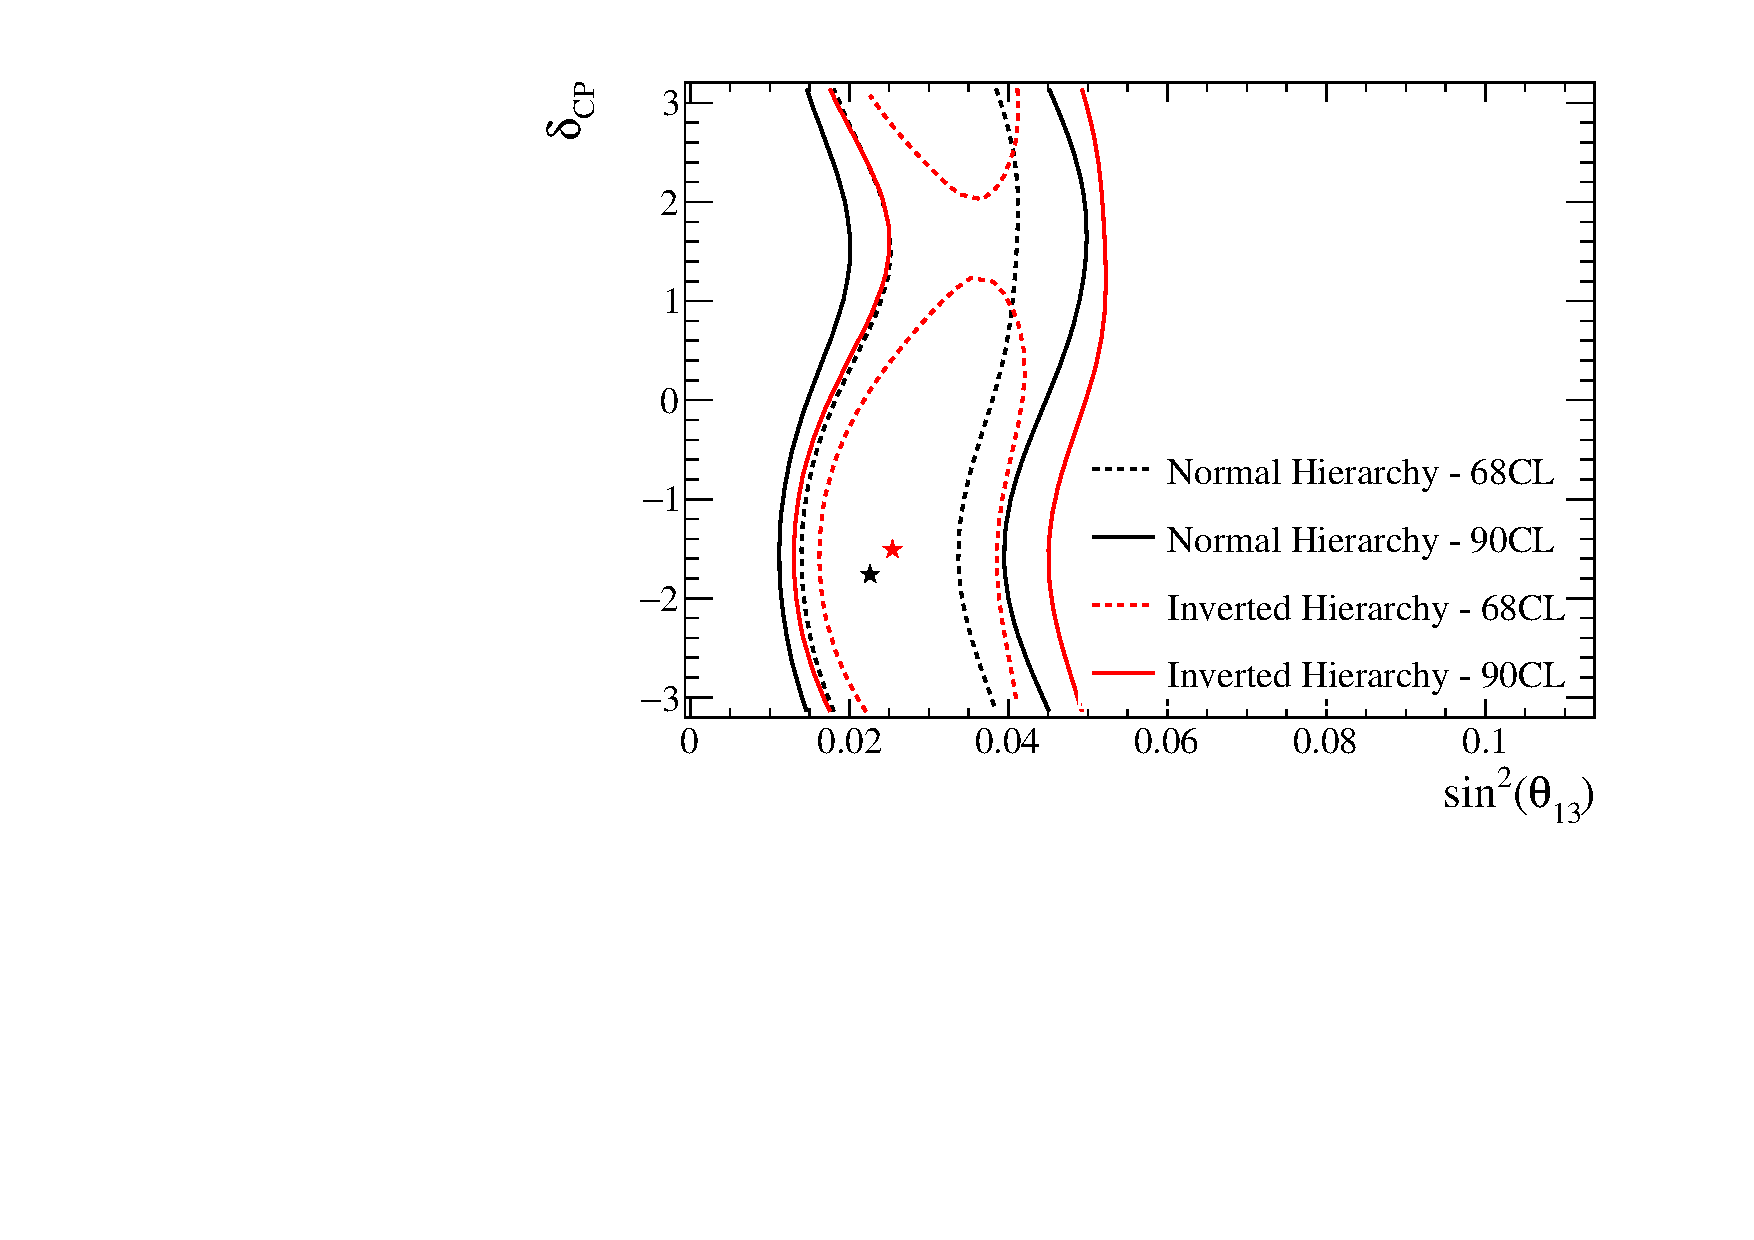
\includegraphics[width=0.9\textwidth]{./joint_plots/sensitivities/2D/cp13/cp13_A.pdf}
%\caption{Asimov A T2K only}
%\end{subfigure}
%\begin{subfigure}[b]{0.49\textwidth}
%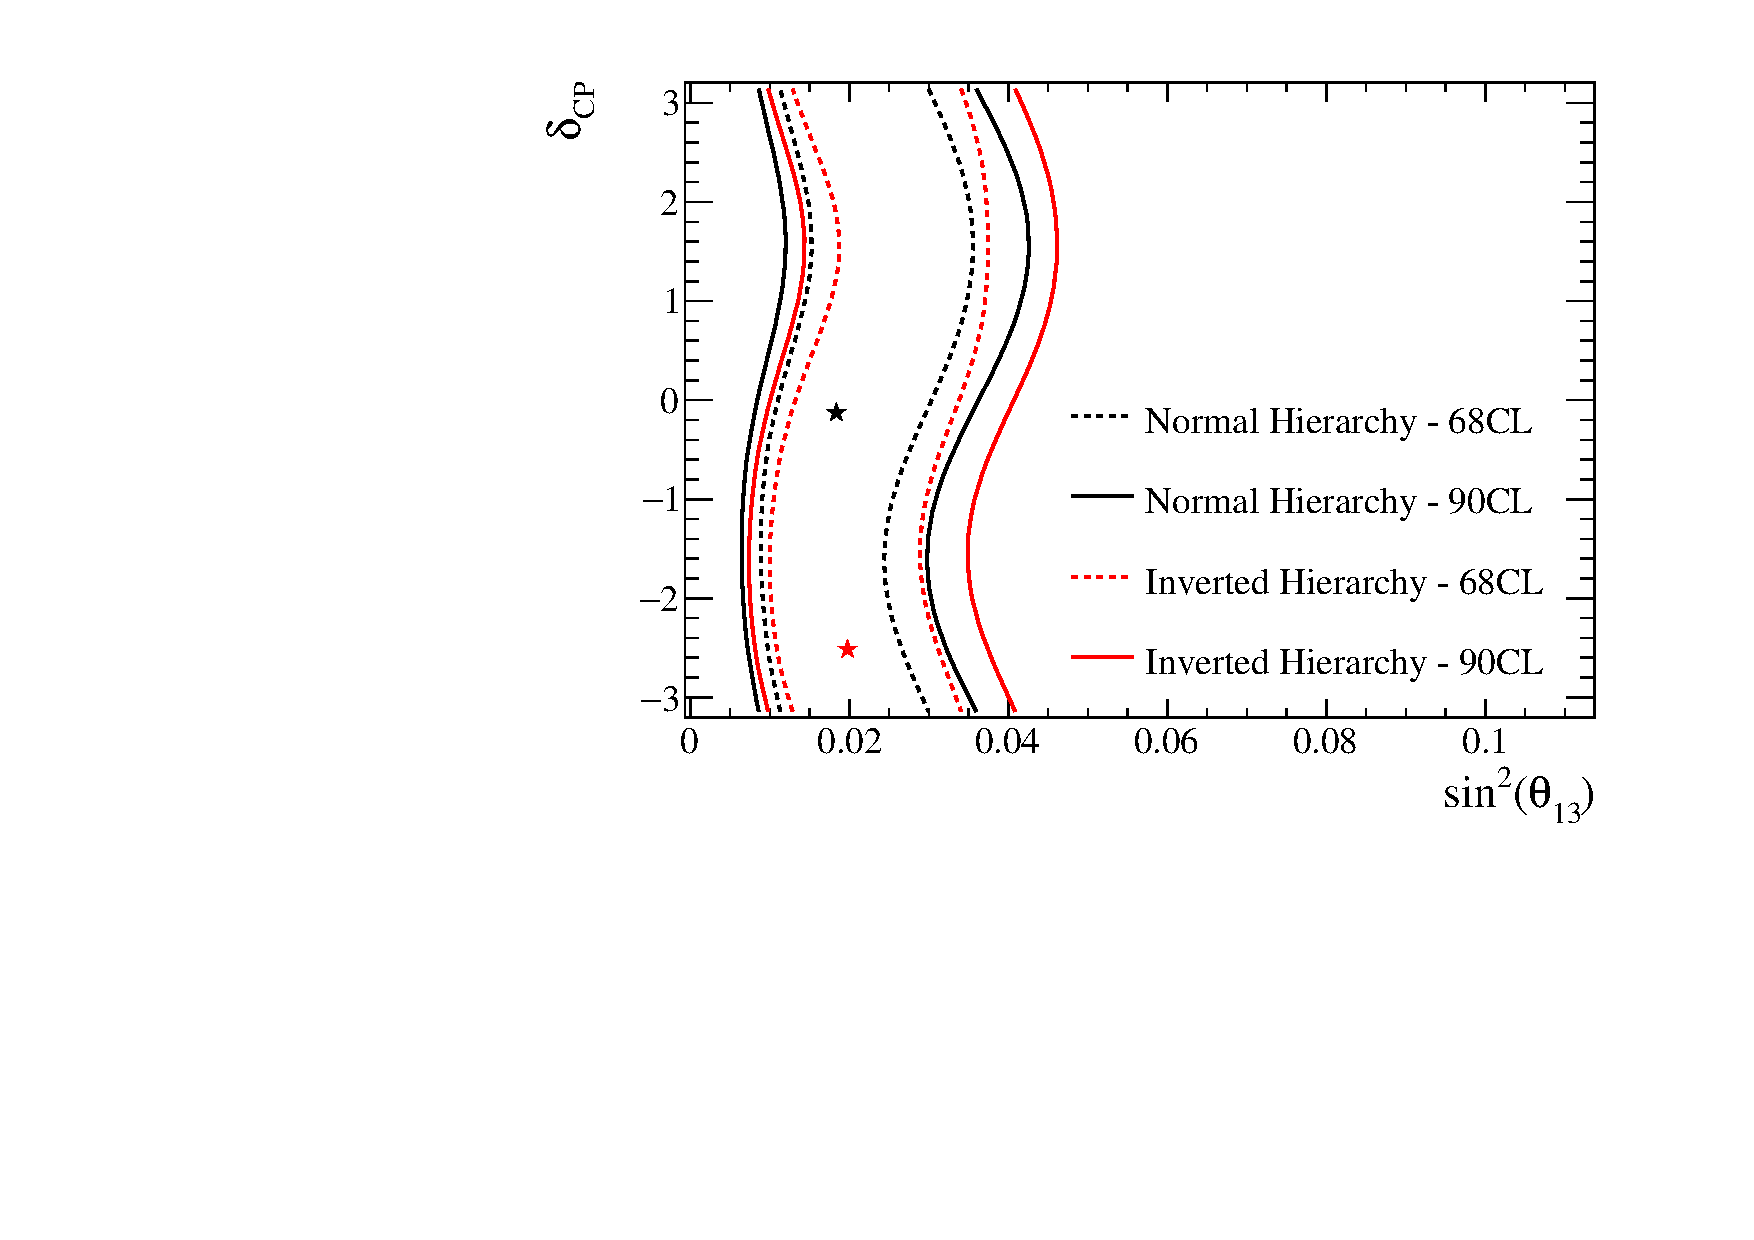
\includegraphics[width=0.9\textwidth]{./joint_plots/sensitivities/2D/cp13/cp13_B.pdf}
%\caption{Asimov B T2K only}
%\end{subfigure}

%\includegraphics[width=0.9\textwidth]{./joint_plots/sensitivities/2D/}
%\includegraphics[width=0.9\textwidth]{./joint_plots/sensitivities/2D/} \\
%\includegraphics[width=0.9\textwidth]{./joint_plots/sensitivities/2D/}
%\includegraphics[width=0.9\textwidth]{./joint_plots/sensitivities/2D/}
\caption {
%{\large{SENSI 2D CONTOURS W/ AND W/O REACTORS}}
The contours at 68\% and 90\% CL for $\sin^2 \theta_{13}$ Vs $\delta_{CP}$
for the Asimov data sets A and B of tab.~\ref{tab:osc_params_joint_asimov} 
corresponding to the Run 1-6 statistics 
is shown.
%is compared to the result obtained by the other analysis groups.
Normal and inverted hierarchy contours are independent.
}
\label{fig:validation_sensi_2d_t2konly}
\end{figure*}

%In Fig.~\ref{fig:validation_data_run14_1d} and~\ref{fig:validation_data_run14_2d} 
%the same $\Delta \chi^2$ distributions for $\delta_{CP}$ 
%as well as the same contours are 
%shown for the Run 1-4 data set and compared to the other analysis groups results.
%
%\begin{figure*}[htb]
%\center
%
\includegraphics[width=0.9\textwidth]{./images/missing_plot-eps-converted-to.pdf}
%
\includegraphics[width=0.9\textwidth]{./images/missing_plot-eps-converted-to.pdf}
%\caption {
%{\large{RUN14 DELTACHISQ 1D DELTACP W/ AND W/O REACTORS}}
%The $\Delta \chi^2$ distribution as a function of $\delta_{CP}$ 
%with reactor constraint (left) and T2K only data (right) 
%for the Run 1-4 data set
%is compared to the result obtained by the other analysis groups.
%The mass hierarchy is minimized:
%both the normal and inverted hierarchy $\chi^2$ distributions 
%are shifted to the same global best-fit $\chi^2$ value,
%which is taken as the minimum between normal and inverted hierarchy.
%}
%\label{fig:validation_data_run14_1d}
%\end{figure*}
%
%\begin{figure*}[htb]
%\center
%
\includegraphics[width=0.9\textwidth]{./images/missing_plot-eps-converted-to.pdf}
%
\includegraphics[width=0.9\textwidth]{./images/missing_plot-eps-converted-to.pdf}
%
\includegraphics[width=0.9\textwidth]{./images/missing_plot-eps-converted-to.pdf}
%\caption {
%{\large{RUN14 2D CONTOURS W/ AND W/O REACTORS}}
%The contours at 68\% and 90\% CL 
%of $\sin^2 \theta_{13}$ Vs $\delta_{CP}$ 
%with reactor constraint (top left) and T2K only data (top right)
%and
%$\sin^2 \theta_{23}$ Vs $|\Delta m^2_{32}|$ 
%with reactor constraint (bottom left) and T2K only data (bottom right)
%for the Run 1-4 data set of tab.~\ref{tab:osc_params_joint} 
%is compared to the result obtained by the other analysis groups.
%Normal and inverted hierarchy contours are independent.
%}
%\label{fig:validation_data_run14_2d}
%\end{figure*}
%
%\vspace{3mm}
%{\huge{
%TODO: ADD COMMENT ON THE SENSITIVITY COMPARISONS
%}}
%\vspace{3mm}


\clearpage



%
% Coverage study of deltaCP
% 

\subsection{Coverage study of $\delta_{CP}$}
\label{sec:coverage_deltacp}

The fit validation is performed also by making coverage studies for the fit of 
the mass hierarchy (MH) and $\delta_{CP}$ with the reactor constraint, which is the main 
result of this release of the $\bar{\nu}/\nu$ joint fit,
in order to understand if the ``Feldman-Cousins method" is needed.
The coverage is defined as the number of times the true values of $\delta_{CP}^{true}$ and $\text{MH}^{true}$, used to generate the toys MC,
is contained in the confidence interval defined by eq.~\ref{eq:condition_cl}:

\begin{equation}
\Delta \chi^2 (\delta_{CP},\text{MH}) = \chi^2 (\delta_{CP}^{true},\text{MH}^{true}) - \chi^2 (\delta_{CP}^{bf},\text{MC}^{bf}) < \Delta \chi^2_{crit}
\label{eq:coverage}
\end{equation}

where $\delta_{CP}^{bf}$ and $\text{MH}^{bf}$ are the best-fit values.
Adopting the ``constant $\Delta \chi^2$" method, the critical value $\Delta \chi^2_{crit} = \Delta \chi^2_{crit}$  
at a certain $X$\% confidence level is used for any value of $\delta_{CP}$ and MH.
Many toys MC are performed (10k) and for each one eq.~\ref{eq:coverage} is tested.
The fit has a good coverage if the number of toys MC,
for which eq.~\ref{eq:coverage} is satisfied ($N_{toys}^{X}$),
is equal or close to $X$\% within the statistical uncertainty of the number of toys MC.
If the $N_{toys}^{X} > X\%$, then the fit has over-coverage,
that means the confidence intervals should be tighter than what obtained with 
the ``constant $\Delta \chi^2$ method",
while if $N_{toys}^{X} < X\%$, then the fit has under-coverage 
and excludes a wider range of values than in the correct case.
In Fig.~\ref{fig:coverage_dcp} the coverage study 
of $\delta_{CP}$ 1-dimensional fit with reactor constraint
is shown for the true values $\delta_{CP} = -\pi/2, 0, +\pi/2$
and both mass hierarchies.

\begin{figure*}[htb]
\center
\begin{subfigure}[b]{0.49\textwidth}

\includegraphics[width=0.9\textwidth]{./images/missing_plot-eps-converted-to.pdf}
\caption{$\delta_{CP}^{true} = XXX$ with reactor constraint}
\end{subfigure}
\begin{subfigure}[b]{0.49\textwidth}

\includegraphics[width=0.9\textwidth]{./images/missing_plot-eps-converted-to.pdf}
\caption{$\delta_{CP}^{true} = XXX$ with reactor constraint}
\end{subfigure}
\begin{subfigure}[b]{0.49\textwidth}

\includegraphics[width=0.9\textwidth]{./images/missing_plot-eps-converted-to.pdf}
\caption{Critical values done with the ``Feldman-Cousins" method as a function of $\delta_{CP}^{true}$,
compared with constant $\delta \chi^2$ critical values}
\end{subfigure}
\begin{subfigure}[b]{0.49\textwidth}

\includegraphics[width=0.9\textwidth]{./images/missing_plot-eps-converted-to.pdf}
\caption{Coverage as a function of $\delta_{CP}^{true}$}
\end{subfigure}
\caption {
Coverage study of $\delta_{CP}$ with reactor constraint
for the true values $\delta_{CP} = -\pi/2, 0, +\pi/2$
assuming normal hierarchy.
All the other oscillation parameters are marginalised
and the mass hierarchy is kept fixed to normal in the fit.
The statistics corresponds to the Run 1-6 data set.
}
\label{fig:coverage_dcp}
\end{figure*}

\vspace{3mm}
{\huge{
TODO: ADD COMMENT ON COVERAGE STUDY
}}
\vspace{3mm}





%%
%% Pulls study oscillation parameters
%% 
%
%\subsection{Pull study of oscillation parameters}
%\label{sec:pulls}
%
%Pull studies are performed as well 
%for 1-dimensional fits of the oscillation parameters,
%since $1\sigma$ error ranges will be provided for each one independently.
%All the other oscillation parameters are marginalised.
%Since for the current low statistics combined with the non-gaussian behaviour
%they are not expected to be gaussian with mean 0 and pull width 1, but
%to have large deviations, for most of the parameters.
%In particular this is true for $\delta_{CP}$, which is cyclic and the values $\pm \pi/2$ behave like a boundary. 
%
%The performance of the fitter was evaluated using ensembles of 5k toy MC experiments, and these were
%generated with statistical fluctuations and variations of all \NSyst{} systematic parameters.
%Toy ensembles were generated for normal hierarchy, which was kept fixed in the fit, 
%and were fitted using the implemented minimization algorithm as described in sec.~\ref{sec:marginalization}.
%
%Asymmetric errors were calculated by choosing the $\pm 1 \sigma$ error as
%the range of free parameter values that satisfy eq.~\ref{eq:coverage}
%with $\Delta \chi^2 = 1$, i.e. the critical value of the $1\sigma$ CL
%(``constant $\Delta \chi^2$ method").
%
%For a free parameter $\theta$ the pull is defined as:
%
%\begin{align}
%&\text{if}( \theta_{bf} > \theta_{true} ) ~\text{pull} = \frac{ \theta_{bf} - \theta_{true}}{\sigma^-_{bf}}  \nonumber \\
%&\text{if}( \theta_{bf} < \theta_{true} ) ~\text{pull} = \frac{ \theta_{bf} - \theta_{true}}{\sigma^+_{bf}} 
%\end{align}
%\label{eq:pull_osc}
%
%where $\sigma^+_{bf}$ is the positive best-fit error and
%$\sigma^-_{bf}$ is the negative best-fit error of $\theta$.
%
%The pull study was performed for the oscillation parameters
%$\delta_{CP}$ with reactor constraint, $\sin^2 \theta_{13}$ with T2K only data,
%$\sin^2 \theta_{23}$ with reactor constraint and $|\Delta m^2_{32}|$ with reactor constraint
%for the Asimov data set of Tab.~\ref{tab:osc_params_joint_asimov}
%and is shown in Fig.~\ref{fig:pull_osc}.
%
%\begin{figure*}[htb]
%\center
%
\includegraphics[width=0.9\textwidth]{./images/missing_plot-eps-converted-to.pdf}
%
\includegraphics[width=0.9\textwidth]{./images/missing_plot-eps-converted-to.pdf}
%
\includegraphics[width=0.9\textwidth]{./images/missing_plot-eps-converted-to.pdf}
%
\includegraphics[width=0.9\textwidth]{./images/missing_plot-eps-converted-to.pdf}
%\caption {
%{\large{PULLS FOR EACH OSCILLATION PARAMETER ASIMOV DATA SET}}
%Pull distributions of 
%$\delta_{CP}$ with reactor constraint, $\sin^2 \theta_{13}$ with T2K only data,
%$\sin^2 \theta_{23}$ with reactor constraint and $|\Delta m^2_{32}|$ with reactor constraint
%assuming normal hierarchy for the Asimov data set of Tab.~\ref{tab:osc_params_joint_asimov}.
%In each fit all the other oscillation parameters are marginalised
%and the mass hierarchy is kept fixed to normal in the fit.
%The statistics corresponds to the Run 1-6 data set.
%The pulls are defined as in Eq.~\ref{eq:pull_osc}.
%}
%\label{fig:pull_osc}
%\end{figure*}
%
%\vspace{3mm}
%{\huge{
%TODO: ADD COMMENT ON PULL STUDY
%}}
%\vspace{3mm}
%



\clearpage



\clearpage

\section {Results of the $\bar{\nu}/\nu$ joint analysis with the Run 1-6 dataset}
\label{sec:results}

The results of the Run 1-6 data set fit
for an exposure 
of \TotalPotNu POT in neutrino mode
and
of \TotalPotNuBar POT in antineutrino mode 
is shown in this chapter.
In \cref{fig:spectra_expVsdata_asimov_A} the predicted spectra of $\mu$-like and $e$-like samples
are compared to the observed data.
In \cref{tab:num_events} the expected and observed number of events in Run 1-6 data set are shown.
The predicted number of events are shown for the oscillation parameters in \cref{tab:osc_params_joint_asimov}
of Asimov data sets A and B.
All the predicted and observed events are in good agreement.
A small excess of events with respect to the expectation is observed in 
the neutrino mode $e$-like samples, though it is still within $1\sigma$ of the statistical uncertainty.
This trend is mostly inherited from the Run 1-4 data set, since only 2 neutrino mode $e$-like events
are observed in Run 5+6.
Furthermore the latest global fit of the reactor experiments 
gives a lower value of $\sin^2 \theta_{13}$ 
with a much smaller uncertainty (see Sec.~\ref{sec:systematics:inputs} and Tab.~\ref{tab:osc_params_joint_asimov}).
It is interesting to see that the number of events of antineutrino mode $e$-like events 
is in perfect agreement with the assumption of $\delta_{CP} = -1.601$,
which is the best-fit value of the Run 1-4 data set. 
This means that, for what concerns the event rate, we expect to see
agreement between neutrino and antineutrino mode data in the fit of $\delta_{CP}$,
though the statistics are not expected to be enough to reject 
$\delta_{CP}=0$ at any significant confidence level.  

The comparison of the confidence intervals obtained by the fit of the Run 1-6 data set
among all the oscillation analysis groups is shown in \cite{Mach3JointFitRun16}.


\clearpage

% Expected distributions with data overlapped

\begin{figure}
\center
%
\includegraphics[width=0.9\textwidth]{./images/missing_plot-eps-converted-to.pdf}
%
\includegraphics[width=0.9\textwidth]{./images/missing_plot-eps-converted-to.pdf}
%
\includegraphics[width=0.9\textwidth]{./images/missing_plot-eps-converted-to.pdf}
%
\includegraphics[width=0.9\textwidth]{./images/missing_plot-eps-converted-to.pdf}
\begin{subfigure}[b]{0.49\textwidth}
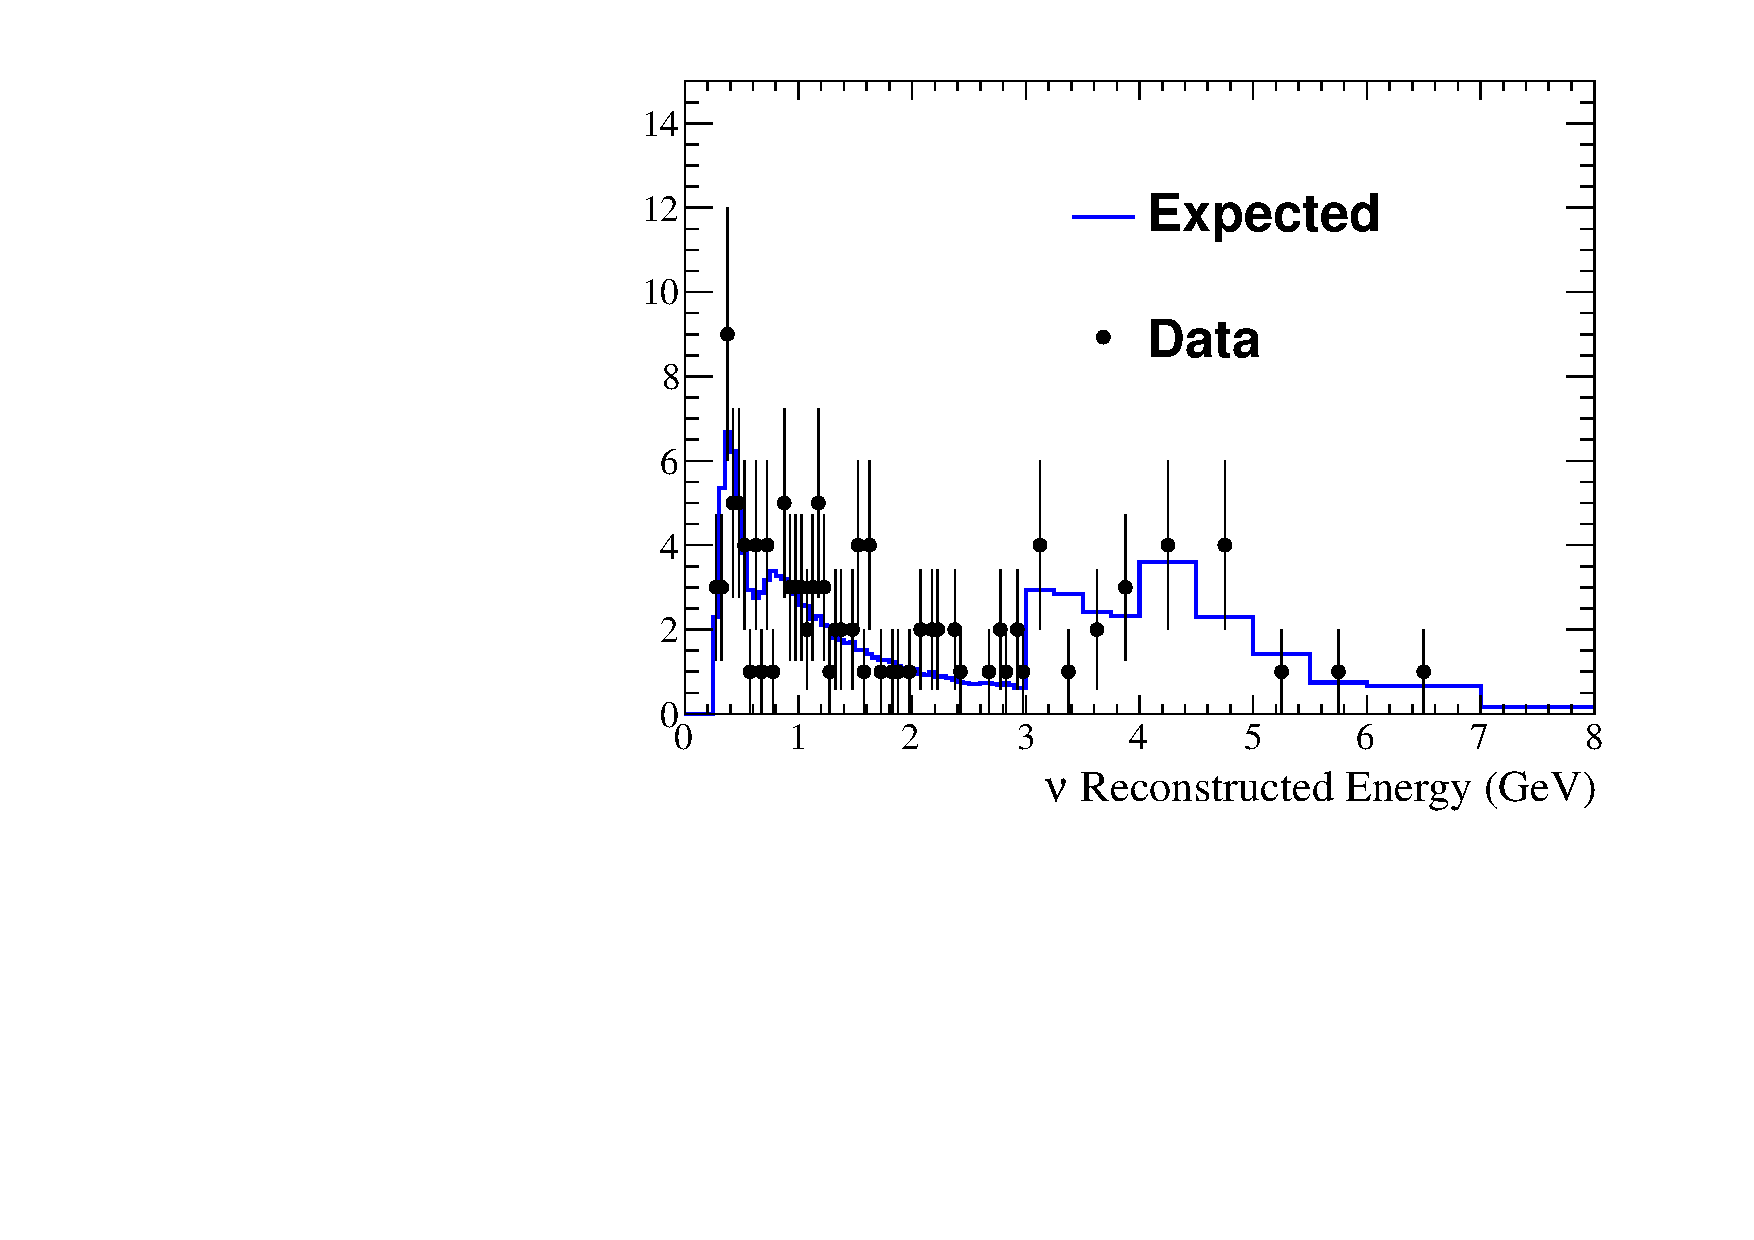
\includegraphics[width=0.9\textwidth]{./joint_plots/data/data_mc_1rmu_tot.pdf}
\caption{Muon-like, neutrino mode}
\end{subfigure}
\begin{subfigure}[b]{0.49\textwidth}
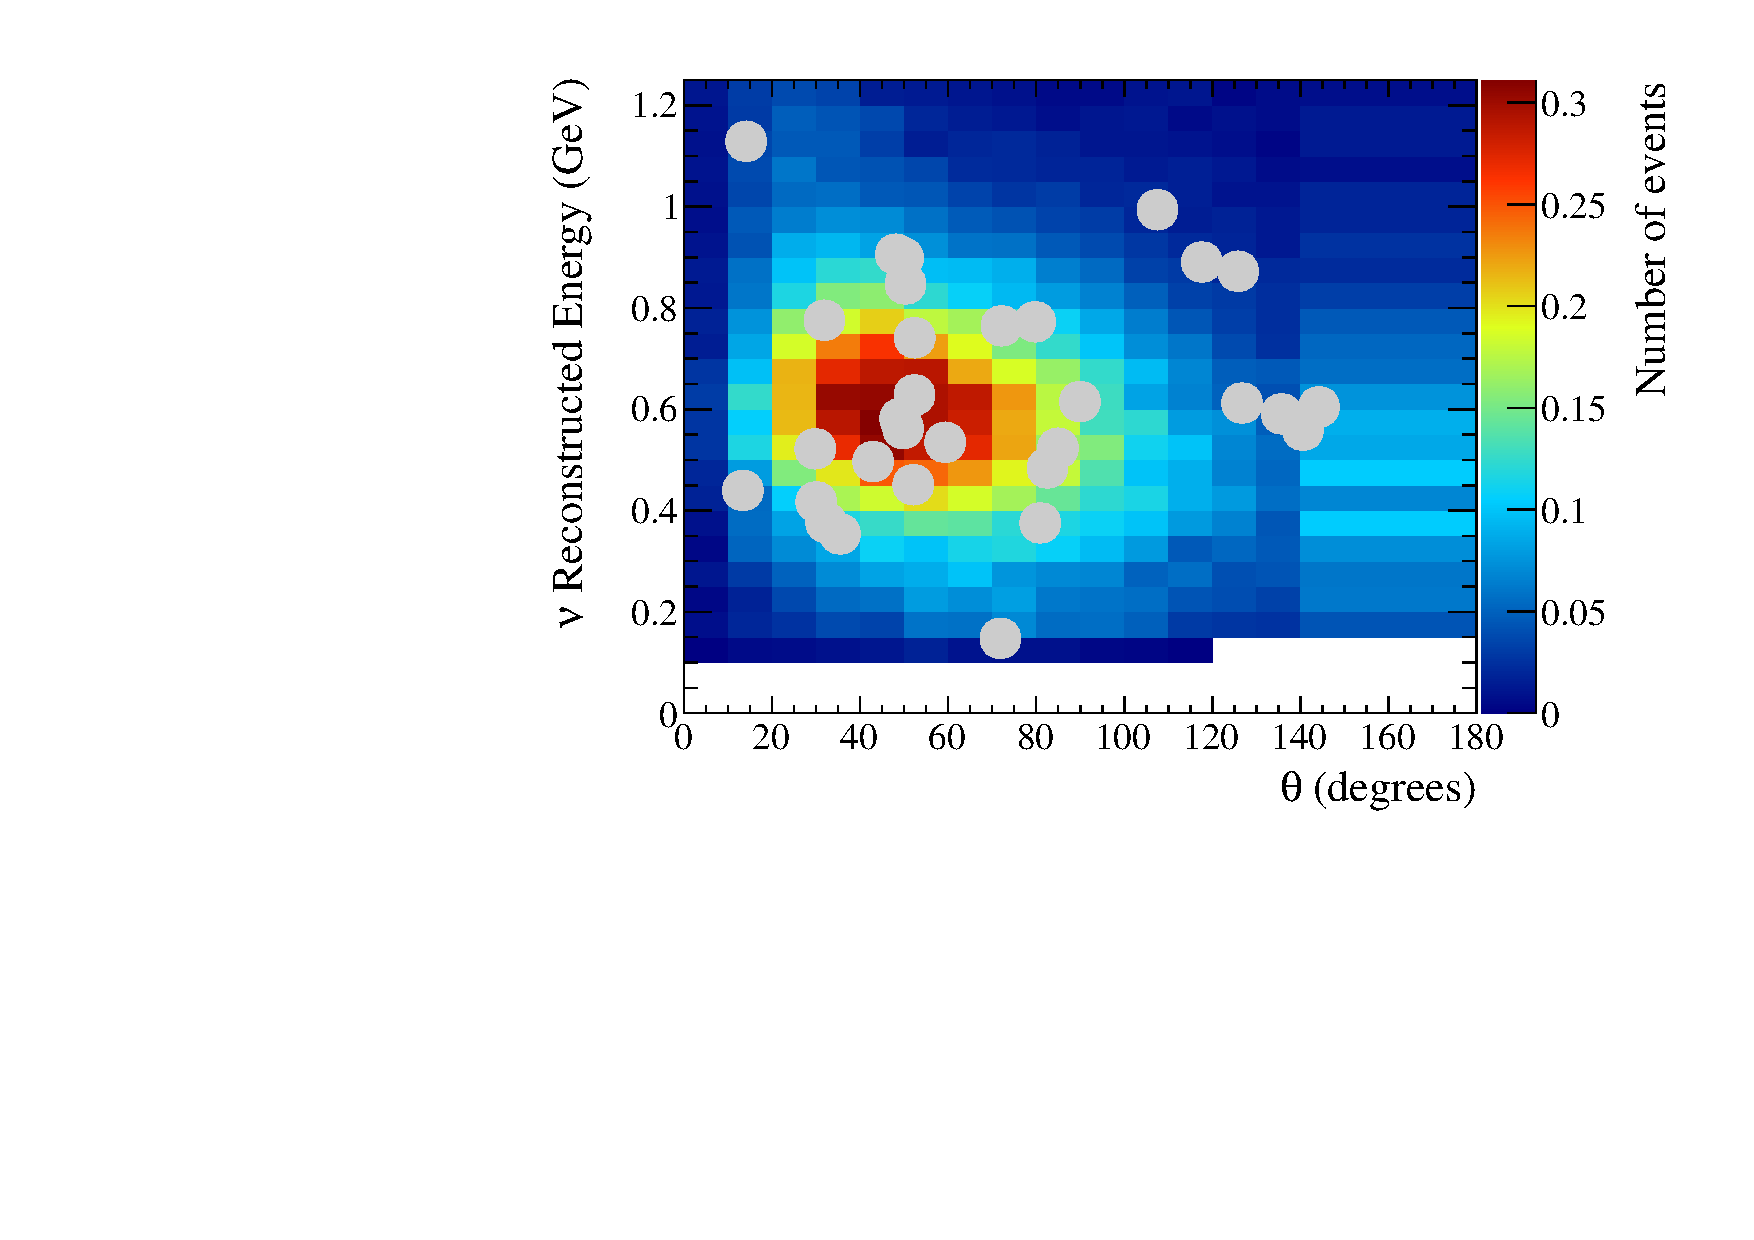
\includegraphics[width=0.9\textwidth]{./joint_plots/data/data_mc_1re_2d_tot.pdf} 
\caption{Electron-like, neutrino mode}
\end{subfigure}
\begin{subfigure}[b]{0.49\textwidth}
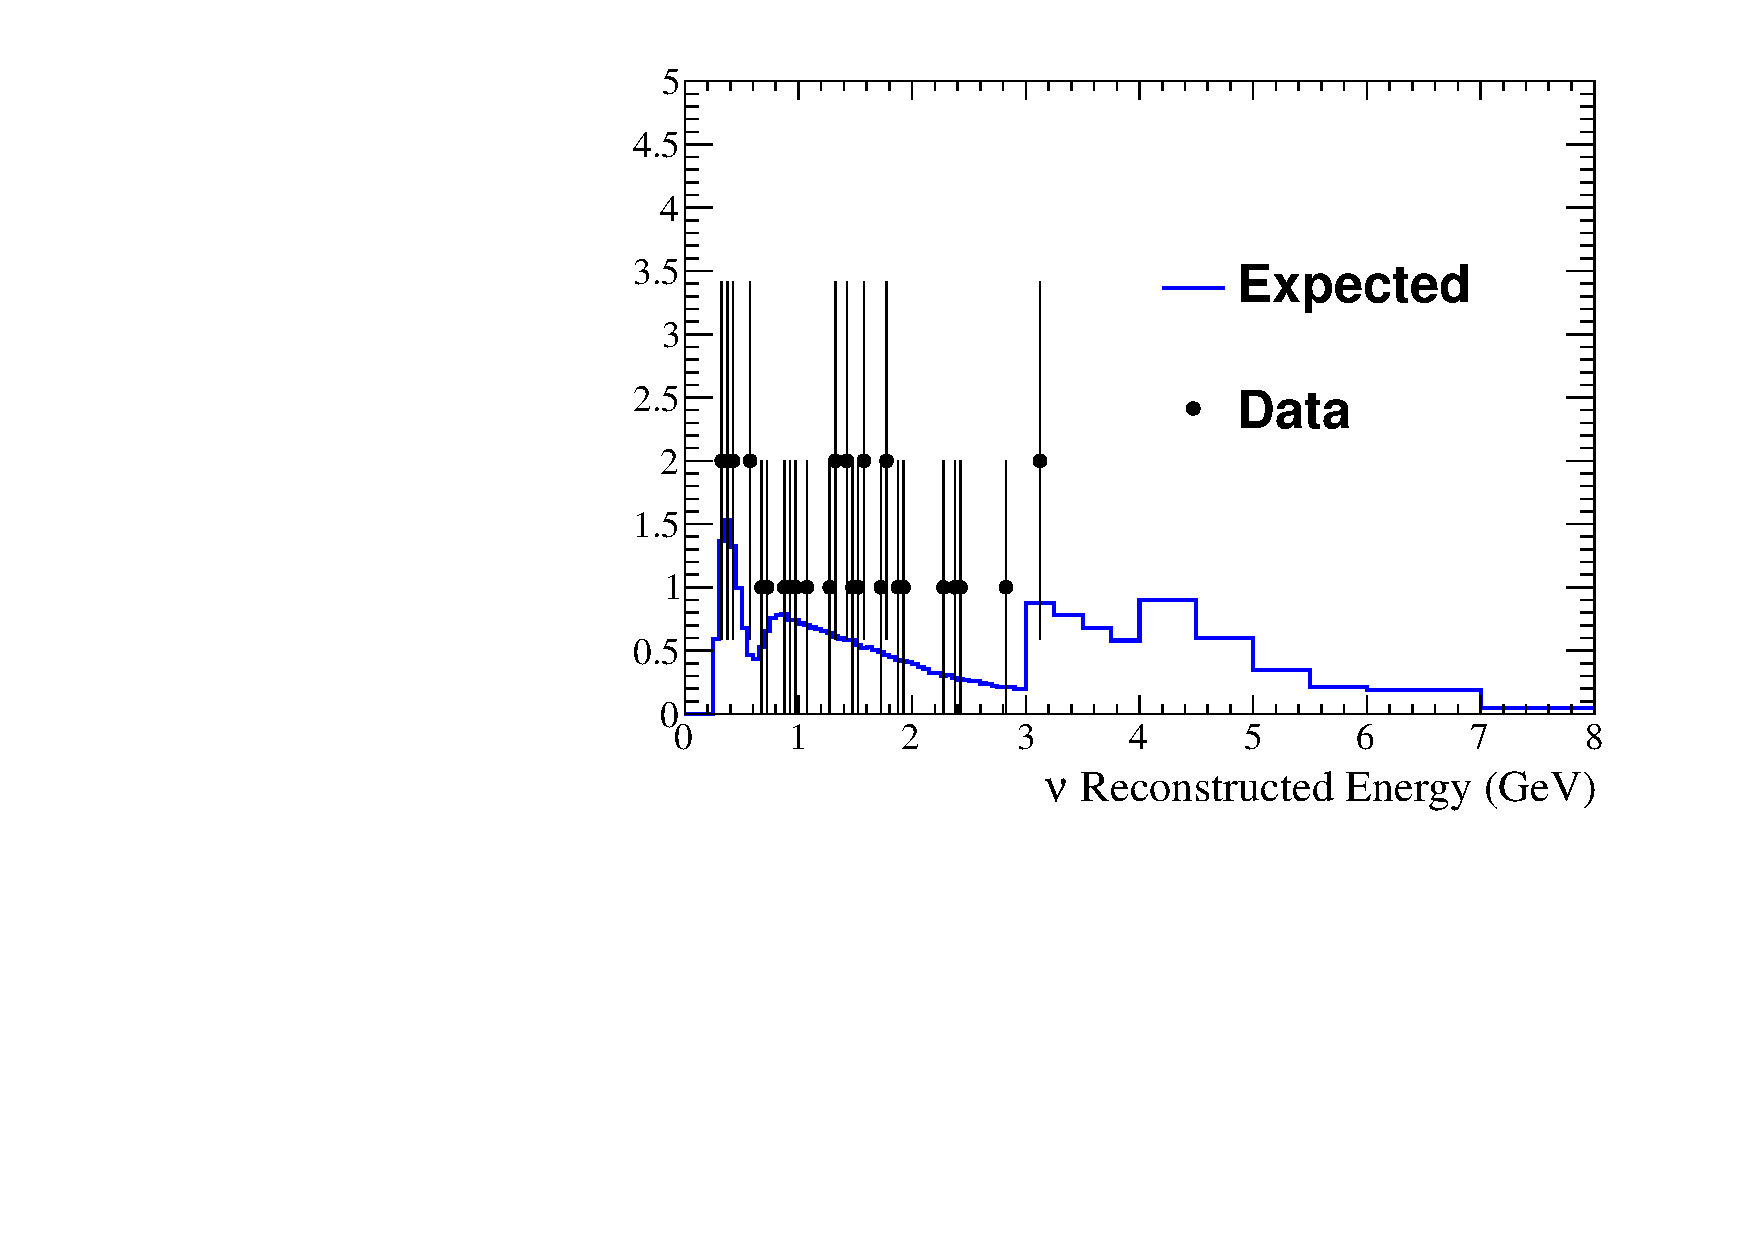
\includegraphics[width=0.9\textwidth]{./joint_plots/data/data_mc_rhc1rmu_tot.pdf}
\caption{Muon-like, antineutrino mode}
\end{subfigure}
\begin{subfigure}[b]{0.49\textwidth}
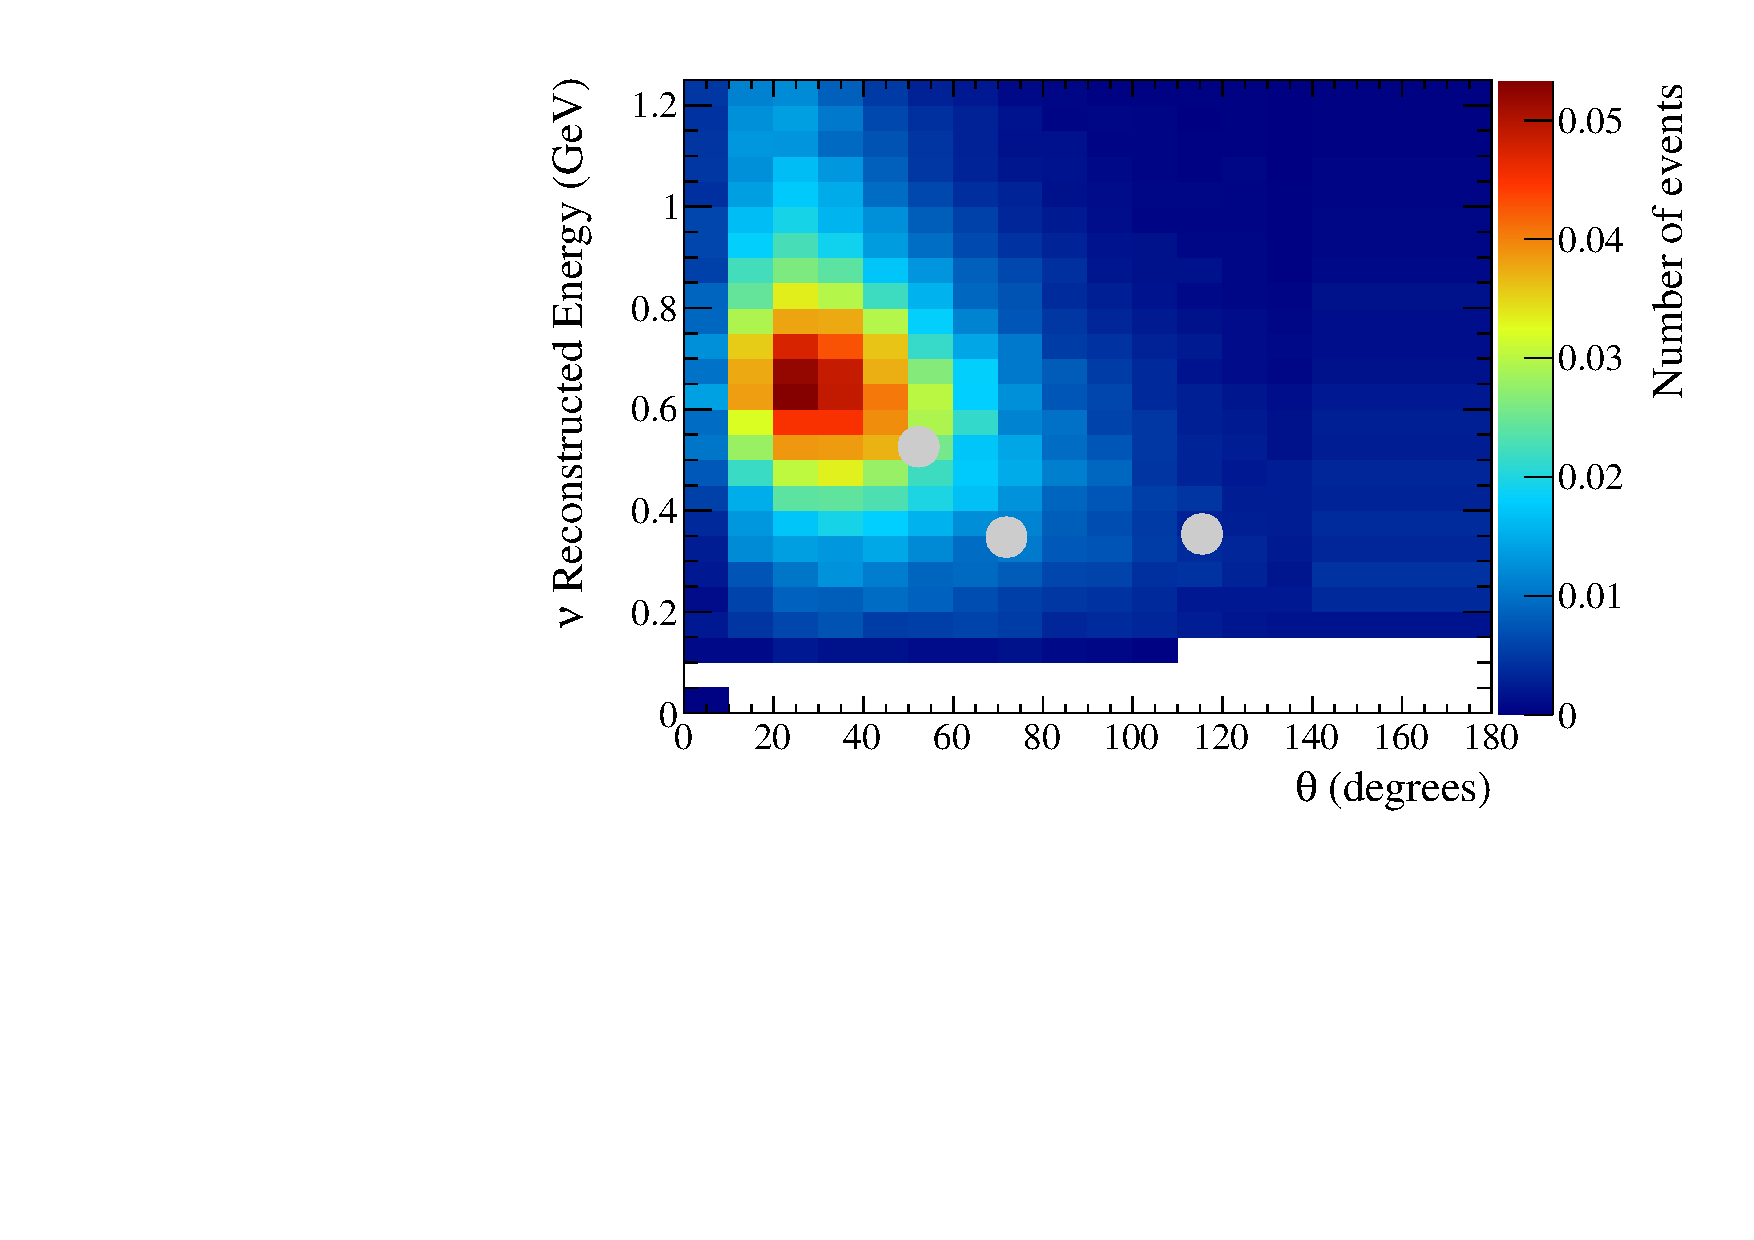
\includegraphics[width=0.9\textwidth]{./joint_plots/data/data_mc_rhc1re_2d_tot.pdf}
\caption{Electron-like, antineutrino mode}
\end{subfigure}
\caption {
%{\large{PREDICTED SPECTRA COMPARED TO DATA}}
The predicted spectra compared to the Run 1-6 dataset (dots),
which corresponds to an exposure 
of \TotalPotNu POT in neutrino mode
and
of \TotalPotNuBar POT in antineutrino mode,
are shown.
The expected distribution corresponds to the oscillation parameters of the Asimov data set A shown in table~\ref{tab:osc_params_joint_asimov}.
The spectra were generated with the systematic parameters measured with the ND280 data 
shown in tab.~\ref{tab:banff_uncertainties_flux_fhc},~\ref{tab:banff_uncertainties_flux_rhc},
~\ref{tab:banff_uncertainties_xsec} and~\ref{tab:banff_uncertainties_skdetfsi}.
}
\label{fig:spectra_expVsdata_asimov_A}
\end{figure}


% Table summarizing the # of observed events in Run 1-6

\begin{table}[htb]
\centering
\begin{tabular}{| c | c | c | c | c | c | c |}
\hline
Beam mode	& Sample		& Exp. Asimov A  	& Exp. Asimov B	& Exp. Not Osc			& Observed 	& Best fit\\
\hline
neutrino	 	& $\mu$-like 	& 125.914			& 130.464 		& 484.737				& 124 		& 125.688 \\
neutrino 		& $e$-like  	& 26.594			& 19.954			& 5.698				& 31 			& 26.969 \\
antineutrino 	& $\mu$-like 	& 34.284			& 35.032			& 99.02				& 34 			& 34.114 \\
antineutrino 	& $e$-like 	& 3.218			& 3.355			& 1.253				& 3 			& 3.344 \\
\hline
\end{tabular}
\caption{
The observed, expected and best-fit number of events in Run 1-6 data set
for an exposure
of \TotalPotNu POT in neutrino mode
and
of \TotalPotNuBar POT in antineutrino mode
are shown 
for each selected sample.
The prediction is produced using the BANFF tuning
and the oscillation parameters shown in Tab.~\ref{tab:osc_params_joint_asimov}.
The total number of events of the best-fit spectra is obtained by using Eq.~\ref{eq:bestfit_spectrum_marg}.
}
\label{tab:num_events}
\end{table}


%--------------------------------------------------------------------------------------
%
% 1-dimensional chisq & best-fit
%
%--------------------------------------------------------------------------------------

\subsection {1-dimensional $\chi^2$ distributions and best-fit}
\label{sec:chisq_1d}


% 1-dimensional contours

The same 1-dimensional $\chi^2$ distributions as in sec.~\ref{sec:sensi} are produced
and shown in Fig.~\ref{fig:joint_data_fit_1d}.
The best-fit value of $\delta_{CP}$ when the reactor constraint is applied is -1.854
not as close to $-\pi/2$ as the Run 1-4 fit result, which best-fit value was -1.601 (see Tab.~\ref{tab:osc_params_joint_asimov}).
However the difference of $\chi^2$ between $\delta_{CP}^{bf}$ (best-fit value) and $\delta_{CP}=-\pi/2$ is smaller than 0.1.
So the result is consistent with $\delta_{CP} = -\pi/2$ as well as the Run 1-4 data fit.
 

Looking at the $\chi^2$ distribution of $\sin^2 \theta_{13}$ with T2K only data
we can see that the reactor measurements are 
in agreement with the T2K data at about $1\sigma$ level if $\delta_{CP} \sim - \pi/2$
and normal hierarchy is assumed.


\begin{figure*}[htb]
\center
\begin{subfigure}[b]{0.49\textwidth}
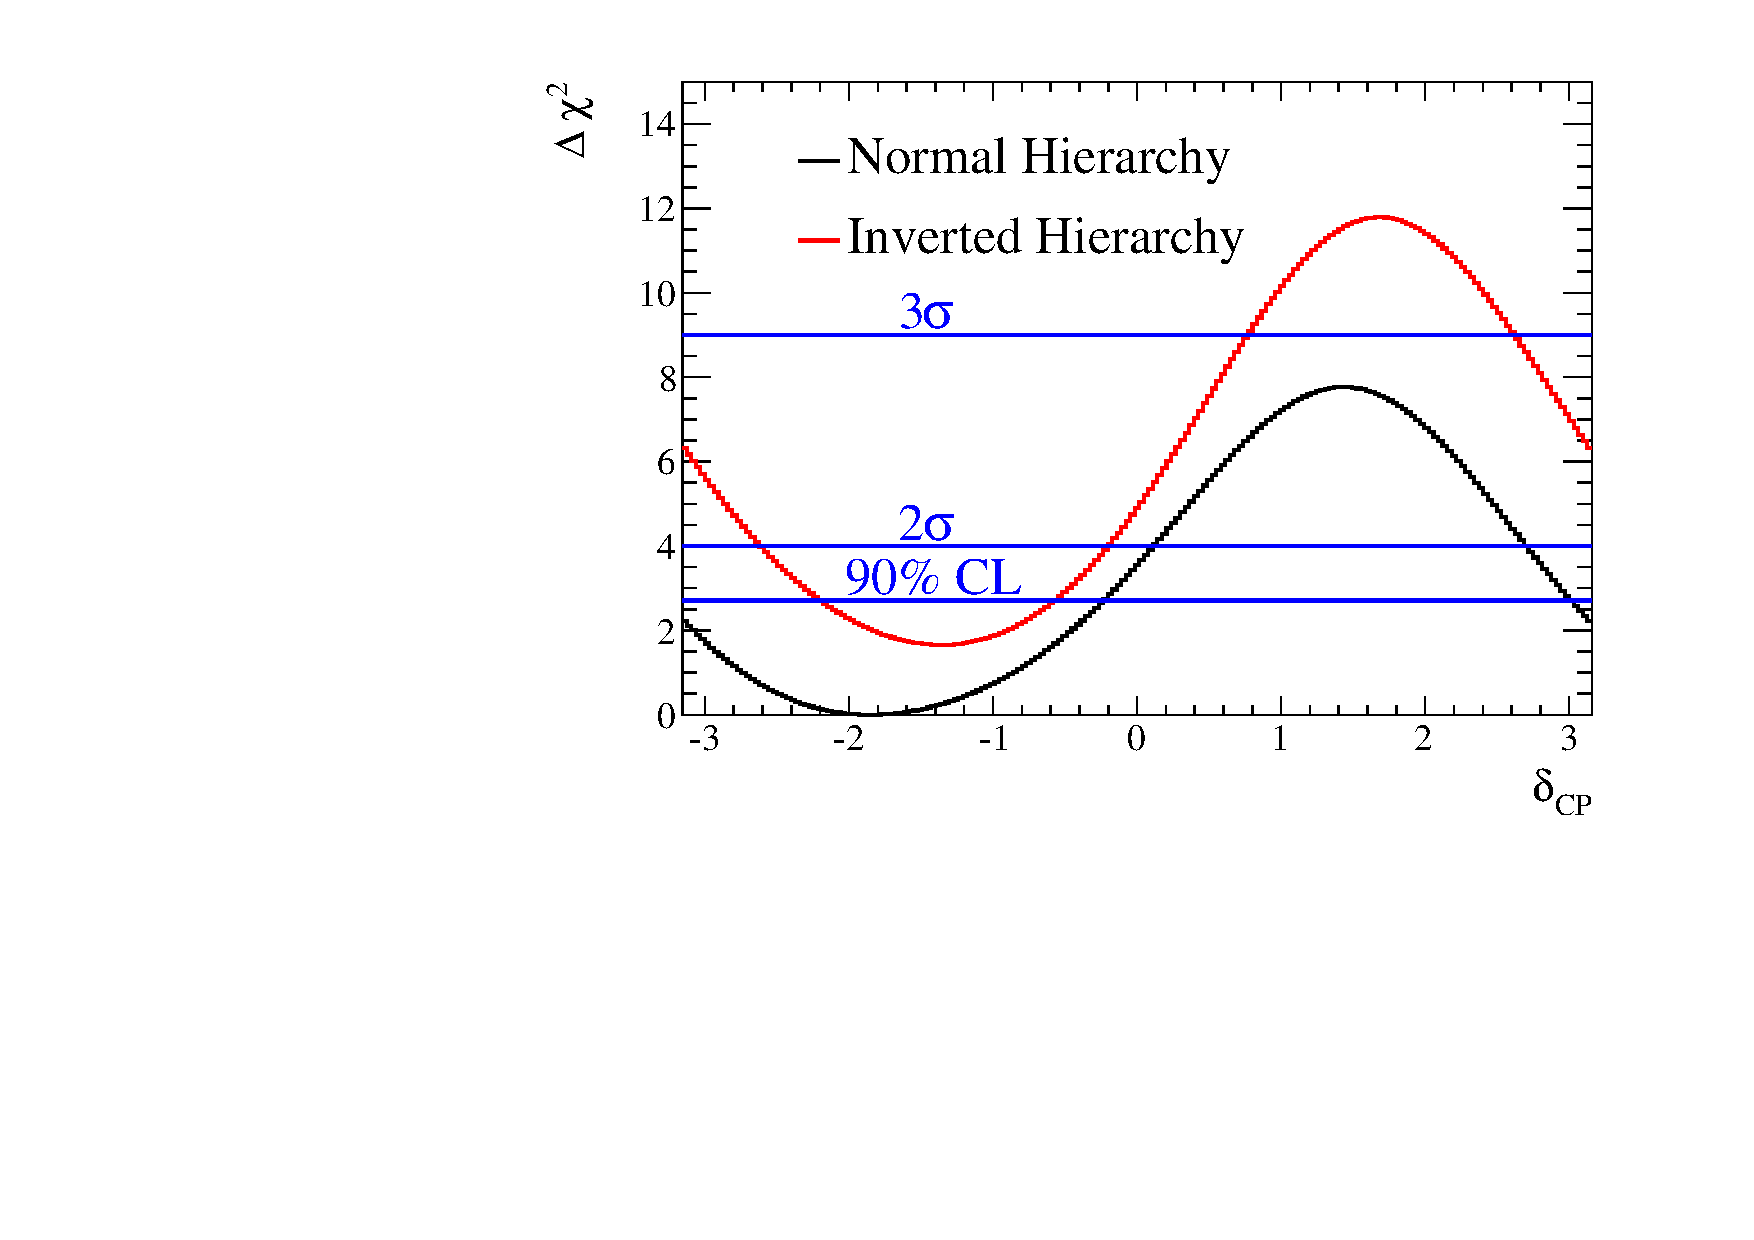
\includegraphics[width=0.9\textwidth]{joint_plots/data_contours/dcp_react_data_constdchisq.pdf}
\caption{$\delta_{CP}$ with reactor constraint}
\label{fig:dcp_fit_with_reactor_data}
\end{subfigure}
\begin{subfigure}[b]{0.49\textwidth}
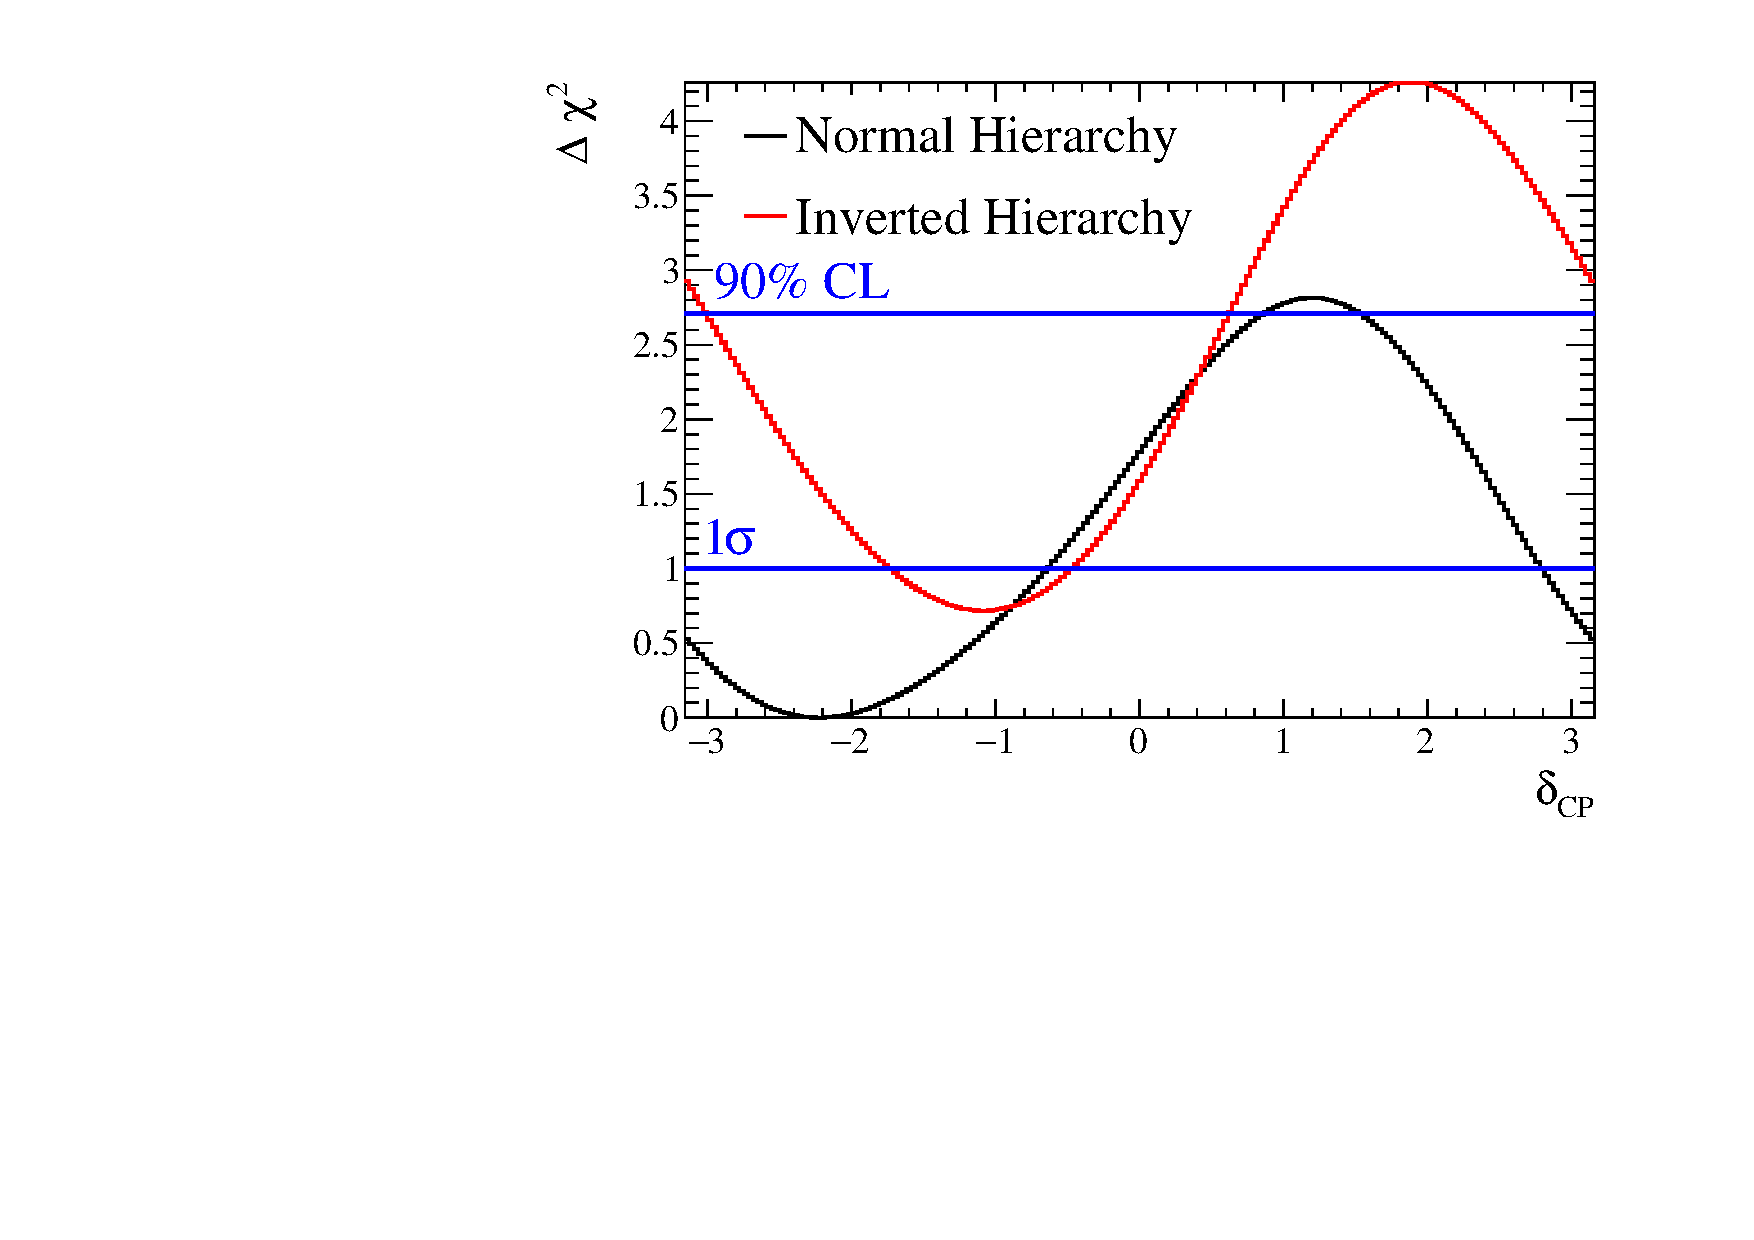
\includegraphics[width=0.9\textwidth]{joint_plots/data_contours/dcp_t2konly_data_constdchisq.pdf}
\caption{$\delta_{CP}$ with T2K data only}
\end{subfigure}
\begin{subfigure}[b]{0.49\textwidth}
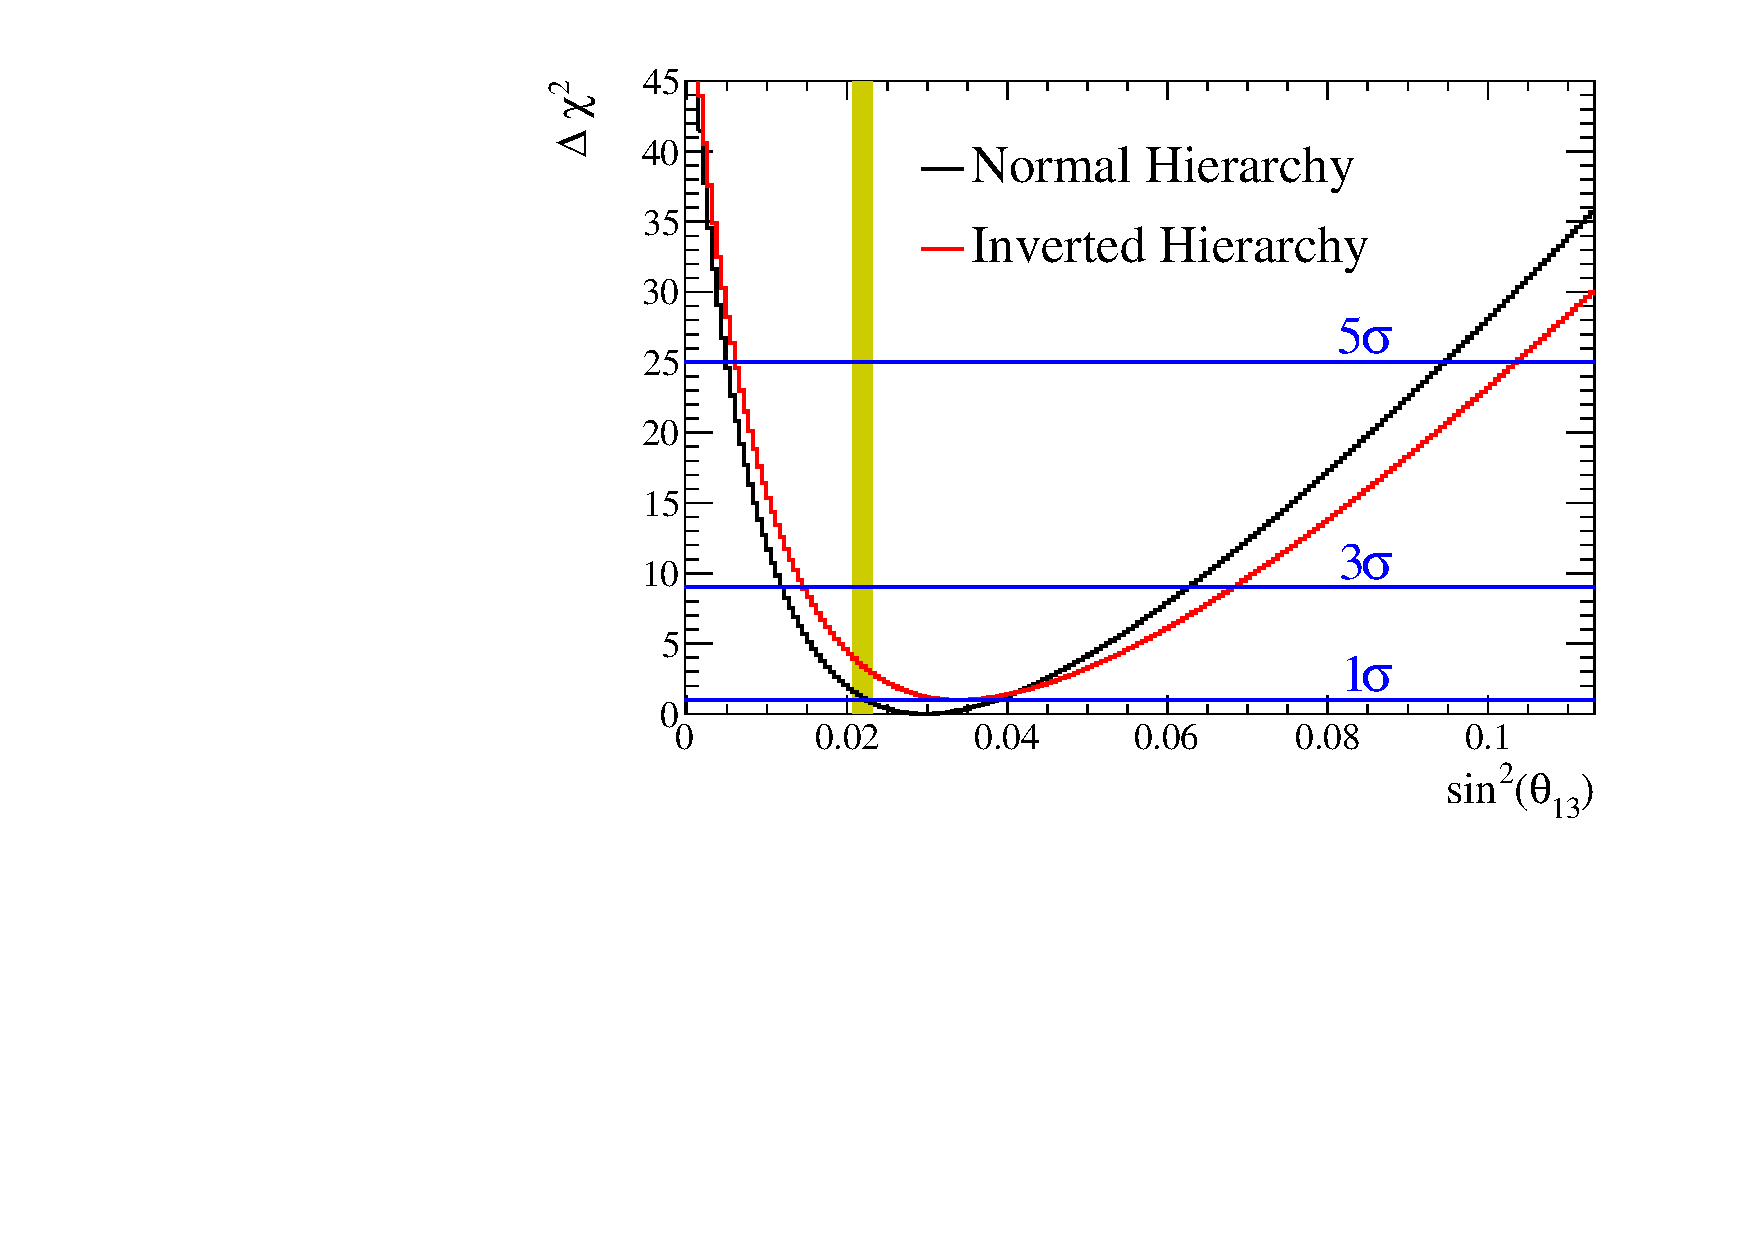
\includegraphics[width=0.9\textwidth]{joint_plots/data_contours/sinsqth13_t2konly_data_constdchisq}
\caption{$\sin^2 \theta_{13}$ with T2K data only}
\end{subfigure}
\begin{subfigure}[b]{0.49\textwidth}
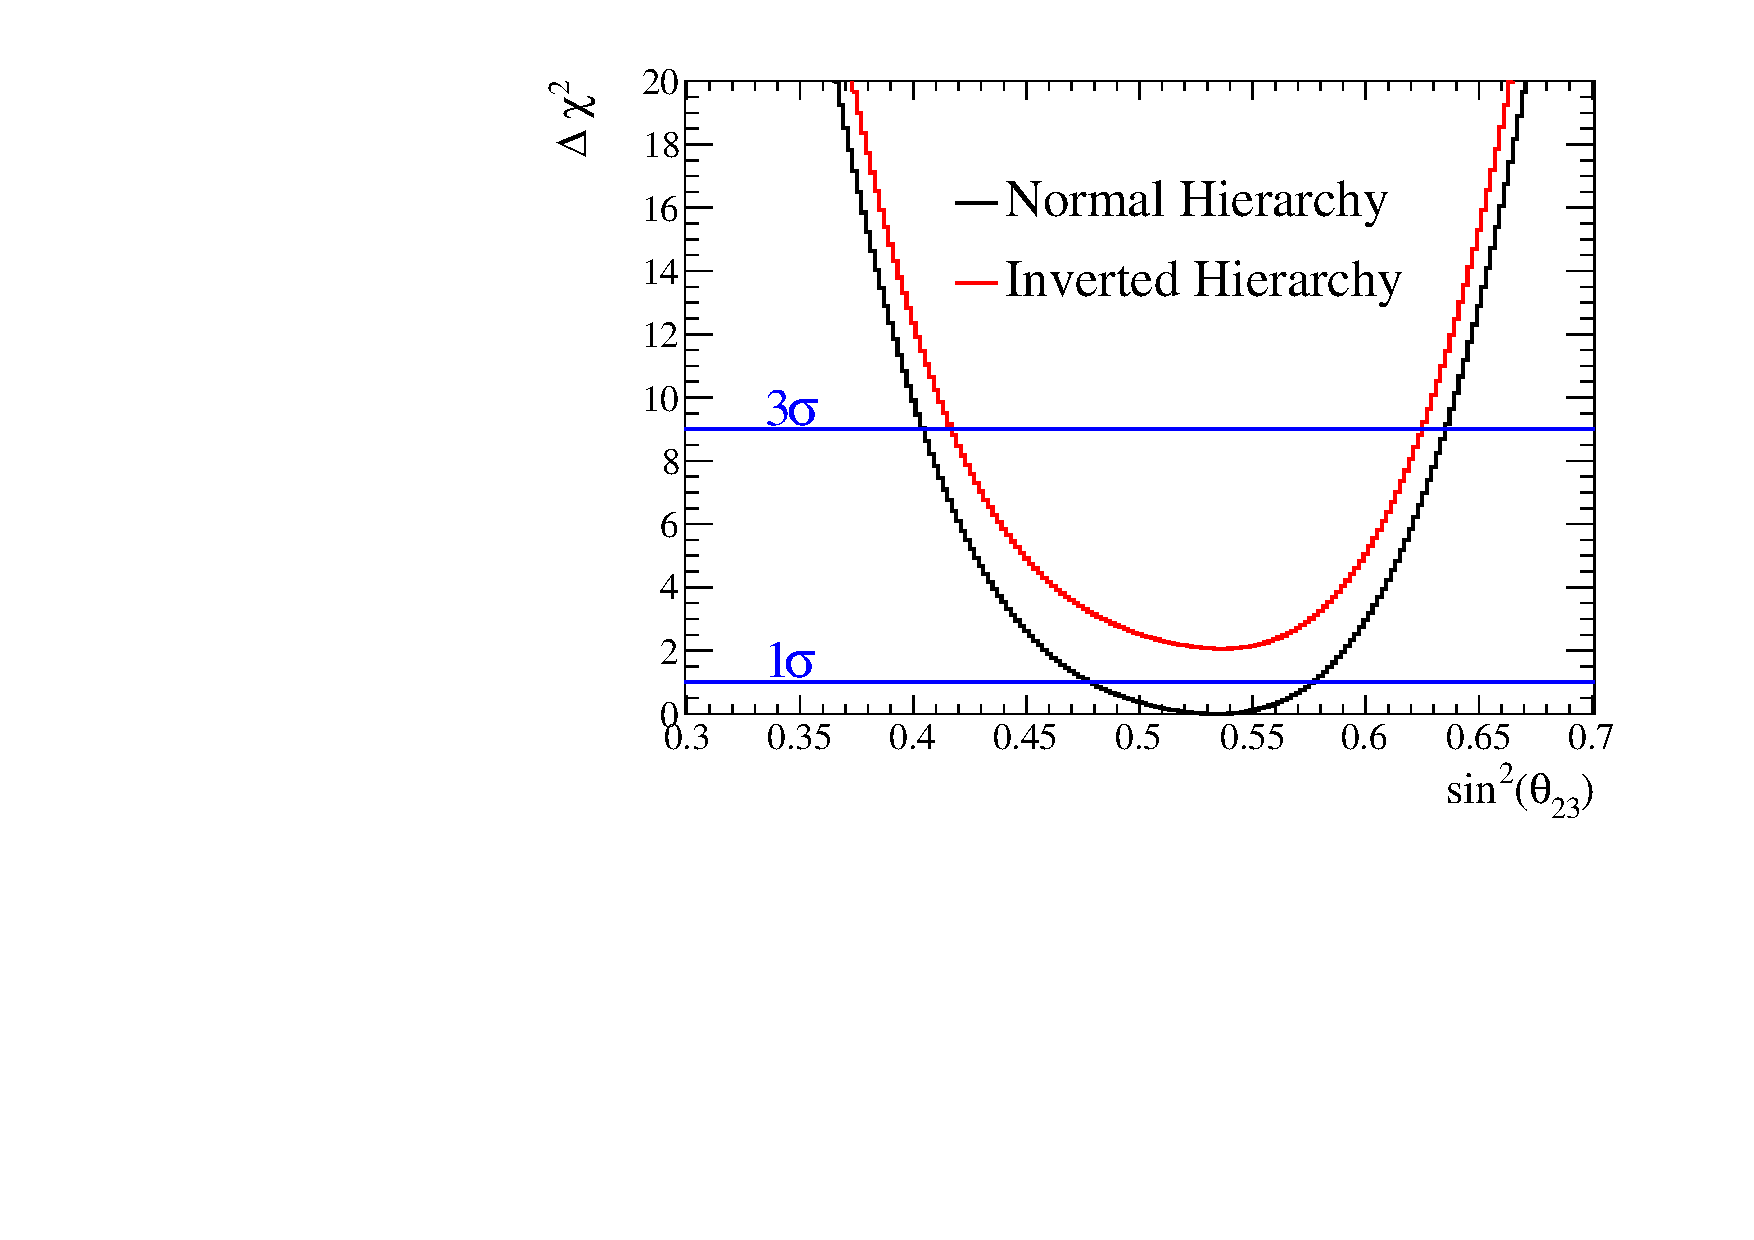
\includegraphics[width=0.9\textwidth]{joint_plots/data_contours/sinsqth23_react_data_constdchisq.pdf}
\caption{$\sin^2 \theta_{23}$ with reactor constraint}
\end{subfigure}
\begin{subfigure}[b]{0.49\textwidth}
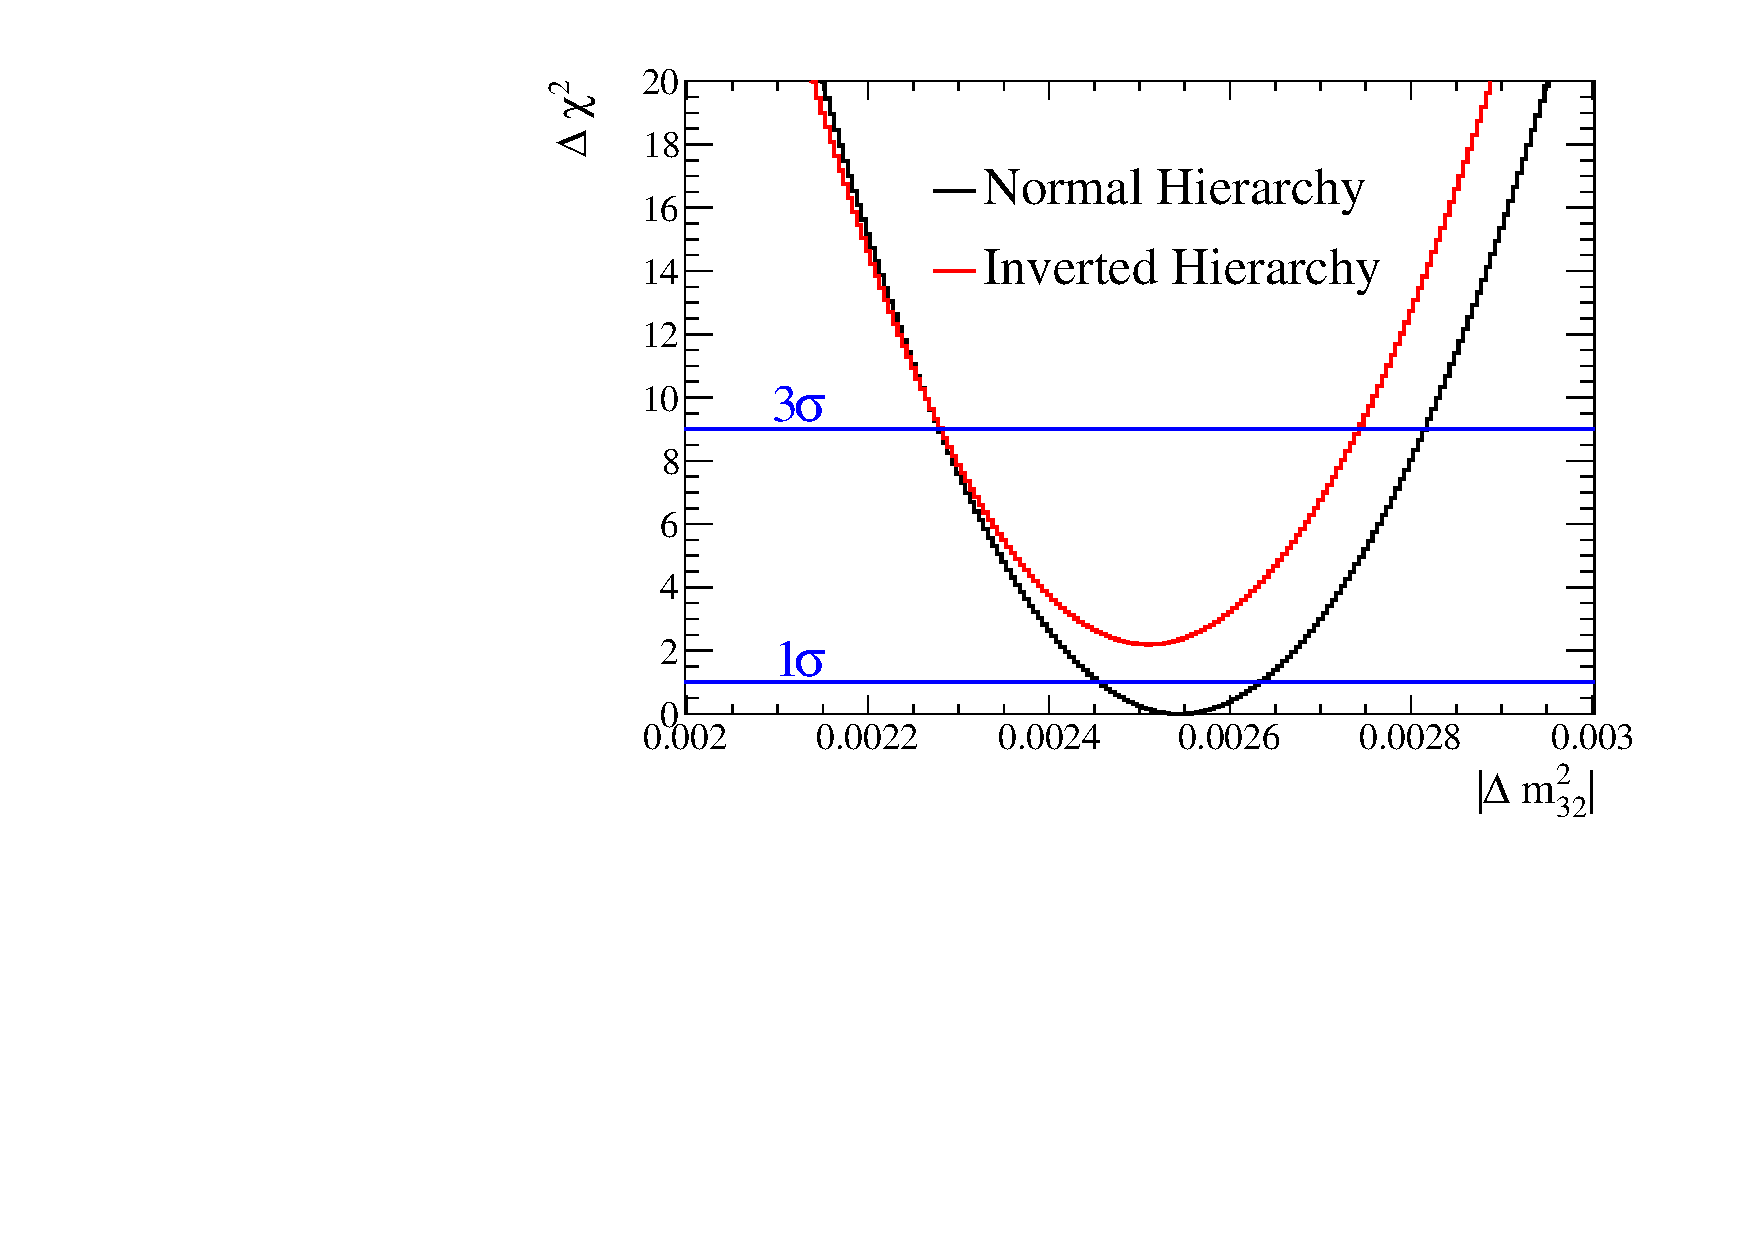
\includegraphics[width=0.9\textwidth]{joint_plots/data_contours/dmsq_react_data_constdchisq.pdf}
\caption{$\Delta m^2_{32}$ ($\Delta m^2_{13}$) with reactor constraint}
\end{subfigure}
\caption{
%    \huge{TO UPDATE} % caption is already ok
%{\large{MEASURED 1D DELTACHISQ DISTRIBUTIONS}}
Measured $\Delta \chi^2$ distributions
with the full run 1-6 data set.
Both normal (black) and inverted (red) hierarchies are shown. 
%Both 68\% (dashed line) and 90\% CL (solid line) are shown.
%For $\delta_{CP}$ confidence intervals are performed using the
%\emph{Feldman-Cousins} method,
%while for the other oscillation parameters
The \emph{constant} $\Delta \chi^2$ method is used. %(see app.~\ref{app:method_cl}).
Both normal and inverted hierarchy $\Delta \chi^2$ distributions are shifted with respect to the same global minimum. 
All the oscillation parameters which are not parameters of interest
are marginalised using the prior distributions shown in tab.~\ref{tab:marg_binnning}.
The measured $\Delta \chi^2$ distribution as a function of $\sin^2 \theta_{13}$ is compared
with the value given by the global analysis of the reactor measurements,
$\sin^2 \theta_{13} = 0.0219 \pm 0.0012 $
\cite{pdg_2014},
shown by the yellow bar.
}
\label{fig:joint_data_fit_1d}
\end{figure*}


%\vspace{3mm}
%{\huge{
%TODO: ADD COMMENTS ABOUT RESULTS
%}}
%\vspace{3mm}


In Fig.~\ref{fig:joint_dcp_nu_nubar}
the $\chi^2$ distributions as a function of $\delta_{CP}$
with reactor constraint
is obtained by 
running the analysis using either only neutrino 
or antineutrino mode samples for the Run 1-6 data set,
in order to check the compatibility of neutrino and antineutrino mode data.
The result is mainly driven by the excess of the observed number
of events in $e$-like neutrino mode sample compared to what is expected.
Though the significance given by the antineutrino mode samples is still low,
also given by the fact that $\sin^2 \theta_{23}$ is not constrained 
by the antineutrino mode $\mu$-like sample
as much as by  
the neutrino mode $\mu$-like sample,
it is interesting to note that the antineutrino data also prefer 
a value of $\delta_{CP}$ close to $-\pi / 2$.

%\vspace{3mm}
%{\huge{
%TODO: ADD COMMENTS ABOUT COMPARISON OF 
%NEUTRINO AND ANTINEUTRINO FIT OF DELTACP
%}}
%\vspace{3mm}

\begin{figure*}[htb]
\center
%
\includegraphics[width=0.9\textwidth]{./images/missing_plot-eps-converted-to.pdf}
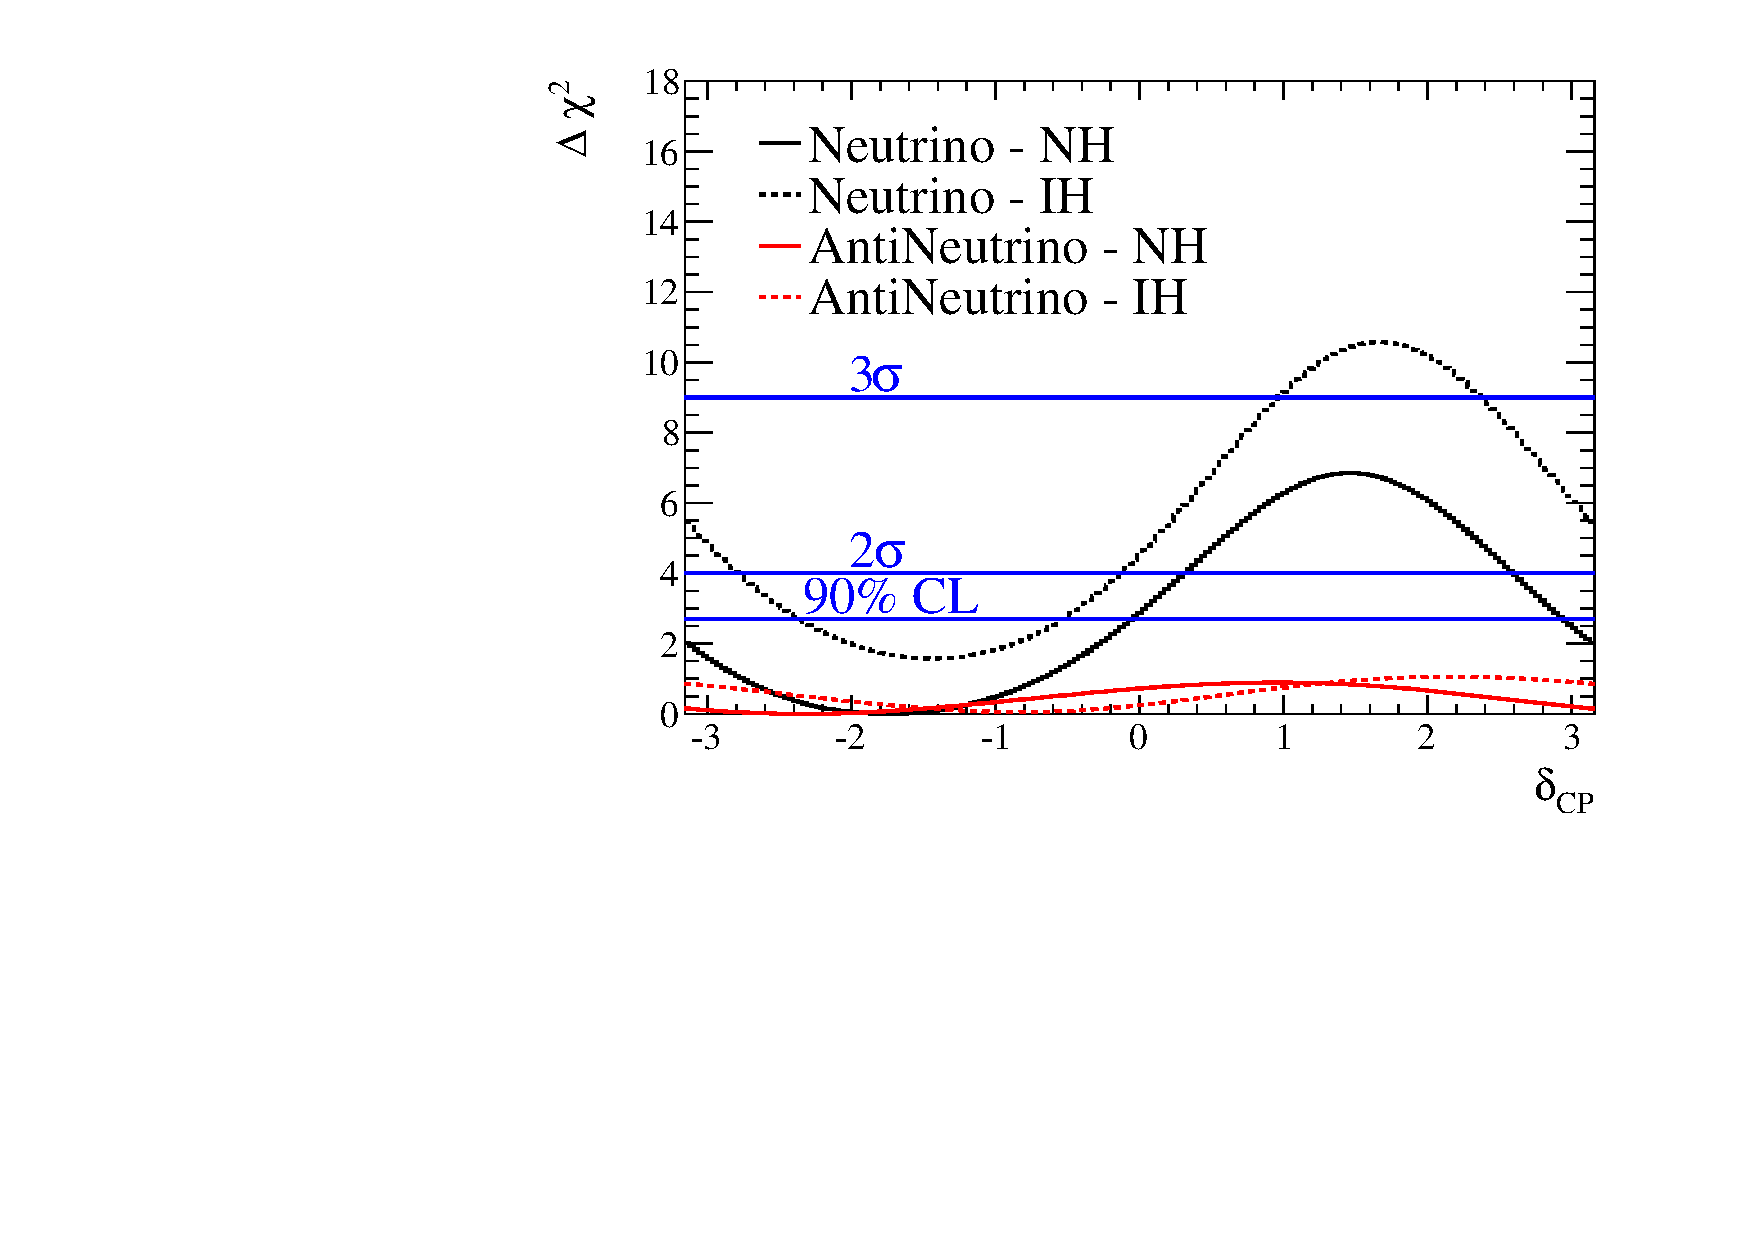
\includegraphics[width=0.5\textwidth]{./joint_plots/data_contours/dcp_react_data_constdchisq_fhcVsrhc.pdf}
\caption{
%{\large{MEASURED 1D DELTACHISQ OF DELTACP FOR 
%NEUTRINO AND ANTINEUTRINO  MODES SEPARATELY}}
Measured $\Delta \chi^2$ distributions
with the full run 1-6 data set
as a function of
$\delta_{CP}$ 
with reactor constraint.
Both normal (black) and inverted (red) hierarchies are shown. 
%Both 68\% (dashed line) and 90\% CL (solid line) are shown.
%For $\delta_{CP}$ confidence intervals are performed using the
%\emph{Feldman-Cousins} method,
%while for the other oscillation parameters
The \emph{constant} $\Delta \chi^2$ method is used. %(see app.~\ref{app:method_cl}).
Both normal and inverted hierarchy $\Delta \chi^2$ distributions are shifted with respect to the same global minimum. 
All the oscillation parameters which are not parameters of interest
are marginalised using the prior distributions shown in tab.~\ref{tab:marg_binnning}.
}
\label{fig:joint_dcp_nu_nubar}
\end{figure*}


In \cref{fig:joint_data_fit_1d_rateonly} the $\chi^2$ distributions as a function of $\delta_{CP}$
is obtained by performing a rate-only analysis; 
instead of using the shape information of the $E_{reco}$ Vs $\theta_l$ spectra,
the total number of events of each sample is fitted, 
reducing the $E_{reco}$ Vs $\theta_l$ template to 1 bin.
Then the best-fit value of $\delta_{CP}$ is -1.602 closer to $-\pi/2$ with respect to the case
where the shape information is used.

\begin{figure*}[htb]
\center
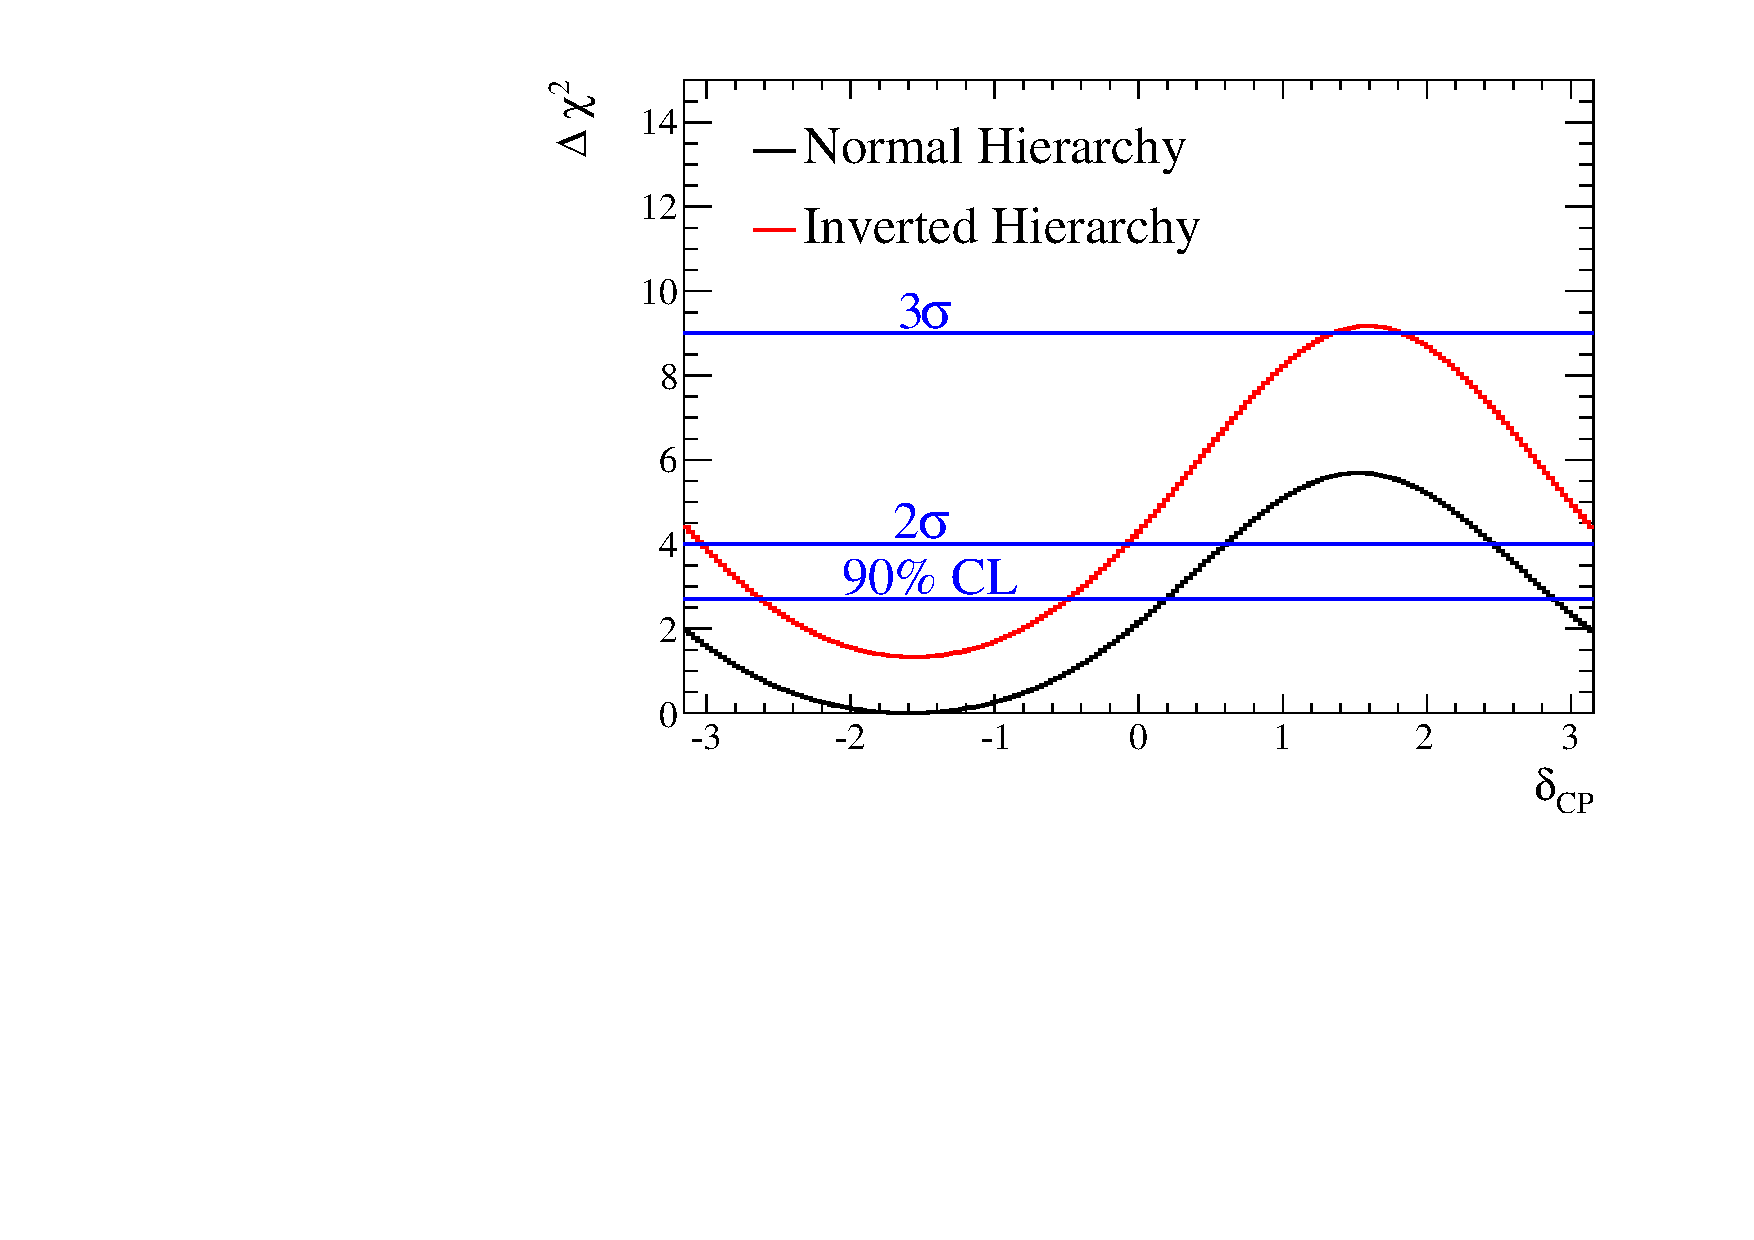
\includegraphics[width=0.5\textwidth]{joint_plots/data_contours/dcp_react_data_constdchisq_rateonly.pdf}
\caption{
%    \huge{TO UPDATE} % caption is already ok
%{\large{MEASURED 1D DELTACHISQ DISTRIBUTIONS}}
Measured $\Delta \chi^2$ distributions
with a rate-only analysis
using the full run 1-6 data set
as a function of
$\delta_{CP}$ 
with reactor constraint.
Both normal (black) and inverted (red) hierarchies are shown. 
%Both 68\% (dashed line) and 90\% CL (solid line) are shown.
%For $\delta_{CP}$ confidence intervals are performed using the
%\emph{Feldman-Cousins} method,
%while for the other oscillation parameters
The \emph{constant} $\Delta \chi^2$ method is used. %(see app.~\ref{app:method_cl}).
Both normal and inverted hierarchy $\Delta \chi^2$ distributions are shifted with respect to the same global minimum. 
All the oscillation parameters which are not parameters of interest
are marginalised using the prior distributions shown in tab.~\ref{tab:marg_binnning}.
}
\label{fig:joint_data_fit_1d_rateonly}
\end{figure*}



In Fig.~\ref{fig:joint_dcp_fc} the confidence intervals obtained with the ``Feldman-Cousins" method
are shown for $\delta_{CP}$ with reactor constraint.
The critical values are calculated as a function of $\delta_{CP}$ as well as the mass hierarchy,
as shown in \cref{sec:cl}.


\begin{figure*}[htb]
\center

\includegraphics[width=0.9\textwidth]{./images/missing_plot-eps-converted-to.pdf}
\caption{
{\large{MEASURED FELDMAN-COUSINS DELTACP W/ REACTORS}}
Measured $\Delta \chi^2$ distributions
with the full run 1-6 data set
as a function of
$\delta_{CP}$ with reactor constraint,
$\delta_{CP}$ with T2K data only,
$\sin^2 \theta_{13}$ with T2K data only,
$\sin^2 \theta_{23}$ with reactor constraint
and
$\Delta m^2_{32}$ ($\Delta m^2_{13}$)
with reactor constraint.
Both normal (black) and inverted (red) hierarchies are shown. 
%Both 68\% (dashed line) and 90\% CL (solid line) are shown.
%For $\delta_{CP}$ confidence intervals are performed using the
%\emph{Feldman-Cousins} method,
%while for the other oscillation parameters
The \emph{constant} $\Delta \chi^2$ method is used. % (see app.~\ref{app:method_cl}).
Both normal and inverted hierarchy $\Delta \chi^2$ distributions are shifted with respect to the same global minimum. 
All the oscillation parameters which are not parameters of interest
are marginalised using the prior distributions shown in tab.~\ref{tab:osc_params_joint_priors}.
The measured $\Delta \chi^2$ distribution as a function of $\sin^2 \theta_{13}$ is compared
with the value given by the global analysis of the reactor measurements,
$\sin^2 \theta_{13} = 0.0219 \pm 0.0012 $
\cite{pdg_2014},
shown by the yellow bar.
}
\label{fig:joint_dcp_fc}
\end{figure*}




% Table of best-fit and 1sigma ranges

In Tab.~\ref{tab:joint_bestfit} the best-fit values as well as the $1\sigma$ ranges for each 
oscillation parameter are shown, for both normal and inverted hierarchy.
The $1\sigma$ ranges are extracted for each oscillation parameter
from the 1-dimensional $\Delta \chi^2$ distributions shown in Fig.~\ref{fig:joint_data_fit_1d},
where one oscillation parameter is free and all the other oscillation as well as the systematic 
parameters are marginalised.
The mass hierarchy is minimized:
for both normal and inverted hierarchy the $1\sigma$ ranges are calculated with respect to the 
same global minimum.
Since this approach is not entirely correct and there does not exist any procedure 
to set more reliable confidence intervals which does not consist of toy MC studies (see \cref{sec:cl_mh}),
the advice to the reader is to give more importance to the difference in $\chi^2_{marg}$
between normal and inverted hierarchies in the respective best-fit points, 
instead of the $1\sigma$ ranges of inverted hierarchy, 
which are smaller by construction.
It is also worth to notice that the $1\sigma$ ranges for normal hierarchy (best-fit)
are set correctly with the constant $\Delta \chi^2$ method in the gaussian approximation.


\begin{table}[htb]
\centering
\begin{tabular}{| c | c | c | c | c || c | c | c | }
\hline
				& {\bf Reactors}		& \multicolumn{3}{c||}{\bf Normal Hierarchy} & \multicolumn{3}{c|}{\bf Inverted Hierarchy} \\
\hline										
\bf Parameter		&				& Best-fit	& $\chi^2_{min}$	& $\pm 1\sigma$ interval  	 	& Best-fit	& $\chi^2_{min}$ 	& $\pm 1\sigma$ interval  \\
\hline
$\delta_{CP}$             & YES      		& -1.854  	& 296.51			& [-2.737; -0.859]			& -1.351	& 298.16			& -	\\
$\delta_{CP}$            & NO        		& -2.231  	& 299.49			& [-$\pi$; -0.640]  \& [2.793;+$\pi$]	& 1.100	& 300.20			& [-1.735;-0.469]			\\
$\sin^2 \theta_{13}$    & NO             	& 0.0299  	& 297.09			& [0.0224; 0.0387]	        		& 0.0339	& 298.09			& -				\\
$\sin^2 \theta_{23}$                      & YES       	& 0.534	& 295.92			& [0.478; 0.577]			& 0.536	& 297.98			& -                 	\\
$\Delta m^2_{32}$ or $\Delta m^2_{13}$  & YES  & 2.545 	& 295.36 			& [2.455; 2.634]			& 2.510 	& 297.56			& -     	\\
($10^{-3} ~\text{eV}^2 / c^4$) 		& YES	& 		&				&						&		&				& \\
\hline
\end{tabular}
\caption{
  %  \huge{TO UPDATE} % caption is already ok
The measured oscillation parameter best-fit
and minimum $\chi^2$ 
values  
as well as the 
$1\sigma$
%68\% 
%and 90\% 
CL intervals are shown,
for both normal and inverted hierarchy. 
The $\pm1\sigma$ interval is obtained by using the 
\emph{constant} $\Delta \chi^2$ method.
All the parameters are measured using the reactor constraint 
$\sin^2 2\theta_{13} = 0.085 \pm 0.005 $
\cite{pdg_2014},
except for $\delta_{CP}$ and $\sin^2 \theta_{13}$.
As explained in \cref{sec:cl_mh}, the gaussian approximation does not work well 
for discrete parameters like the mass hierarchy however, since there is not a clear way
to compute $1\sigma$ ranges for both mass hierarchies without performing
CPU intensive toy MC studies, the constant $\Delta \chi^2$ method is used.
}                                                                                                                                                                                          
\label{tab:joint_bestfit}
\end{table}




% Best-fit spectra

The best-fit spectra, shown in \cref{fig:joint_spectra_bf} are computed as described in sec.~\ref{sec:spectra_bestfit_method}
and are compared to the unoscillated nominal spectra.
For $e$-like samples, where 2-dimensional templates are used,
the projection onto the reconstructed neutrino energy axis is shown.
All the systematic and oscillation parameters are marginalised following the procedure described in sec.~\ref{sec:spectra_bestfit_method},
while $\sin^2\theta_{23}$, $\delta_{CP}$ and the mass hierarchy were fixed to their best-fit values shown in \cref{tab:joint_bestfit}.
Indeed these oscillation parameters have the strongest effect on the measurement,
since $\sin^2\theta_{13}$ is constrained with the reactor measurement.


\begin{figure*}[htb]
\center
\begin{subfigure}[b]{0.49\textwidth}
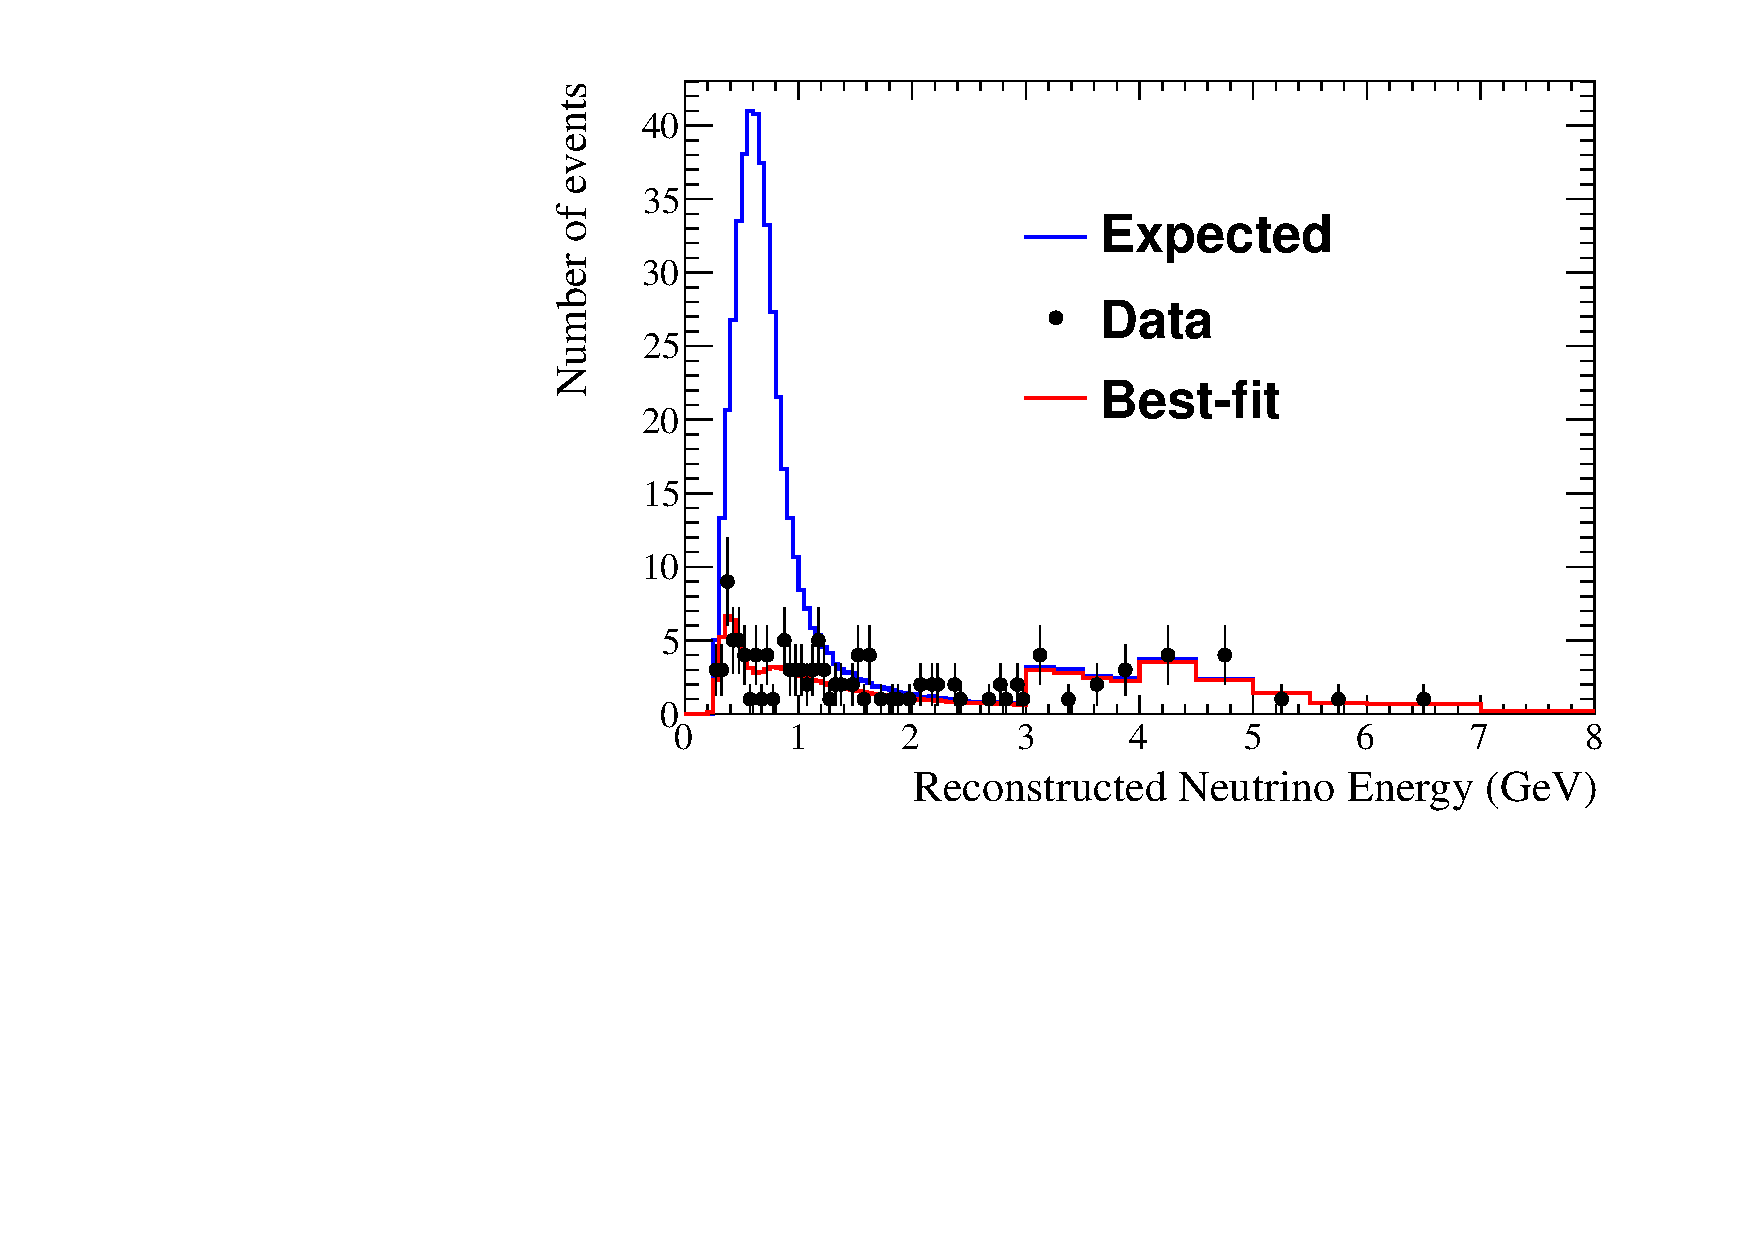
\includegraphics[width=0.9\textwidth]{joint_plots/data/bestfit_marg_sinsqth23Vsdcp_react_1Rmu.pdf}
\caption{Muon-like, neutrino mode}
\end{subfigure}
\begin{subfigure}[b]{0.49\textwidth}
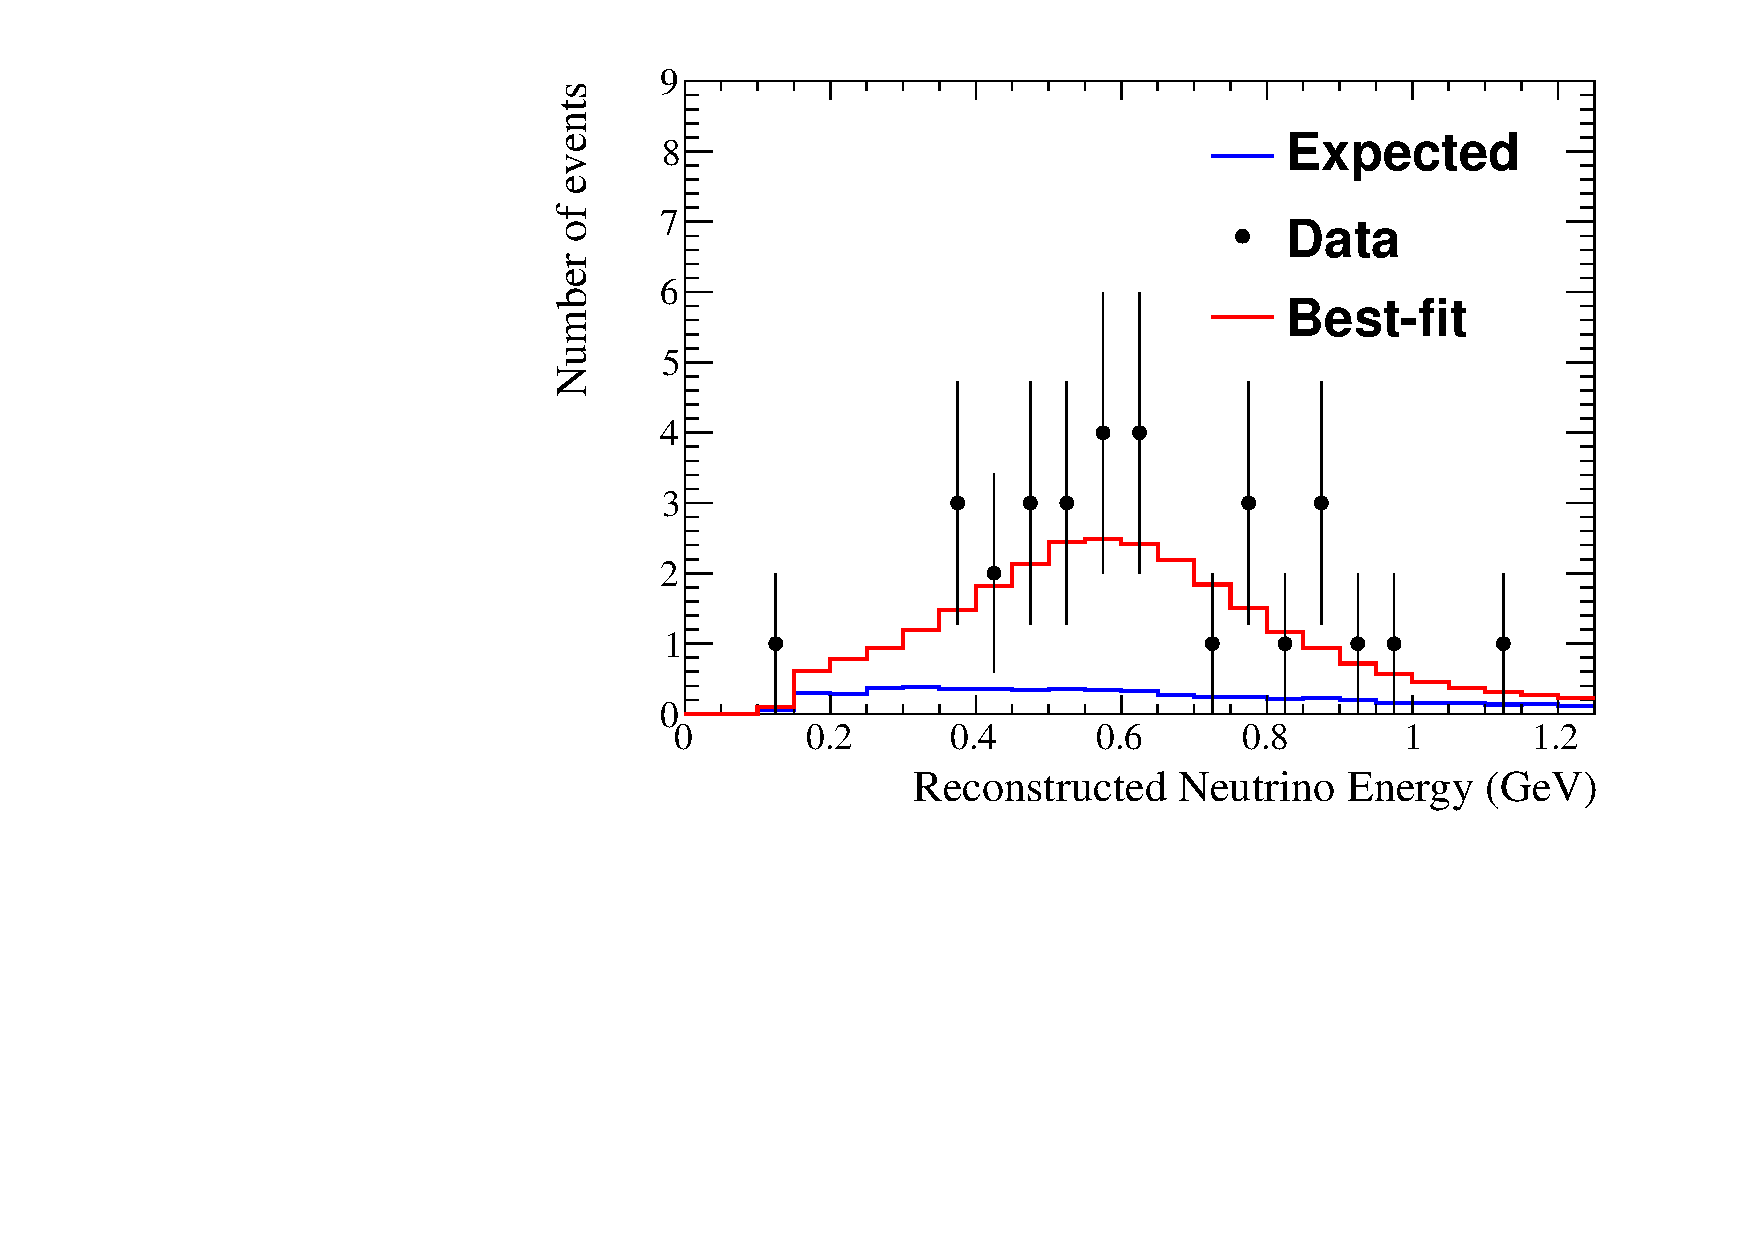
\includegraphics[width=0.9\textwidth]{joint_plots/data/bestfit_marg_sinsqth23Vsdcp_react_1Re.pdf}
\caption{Electron-like, neutrino mode}
\end{subfigure}
\begin{subfigure}[b]{0.49\textwidth}
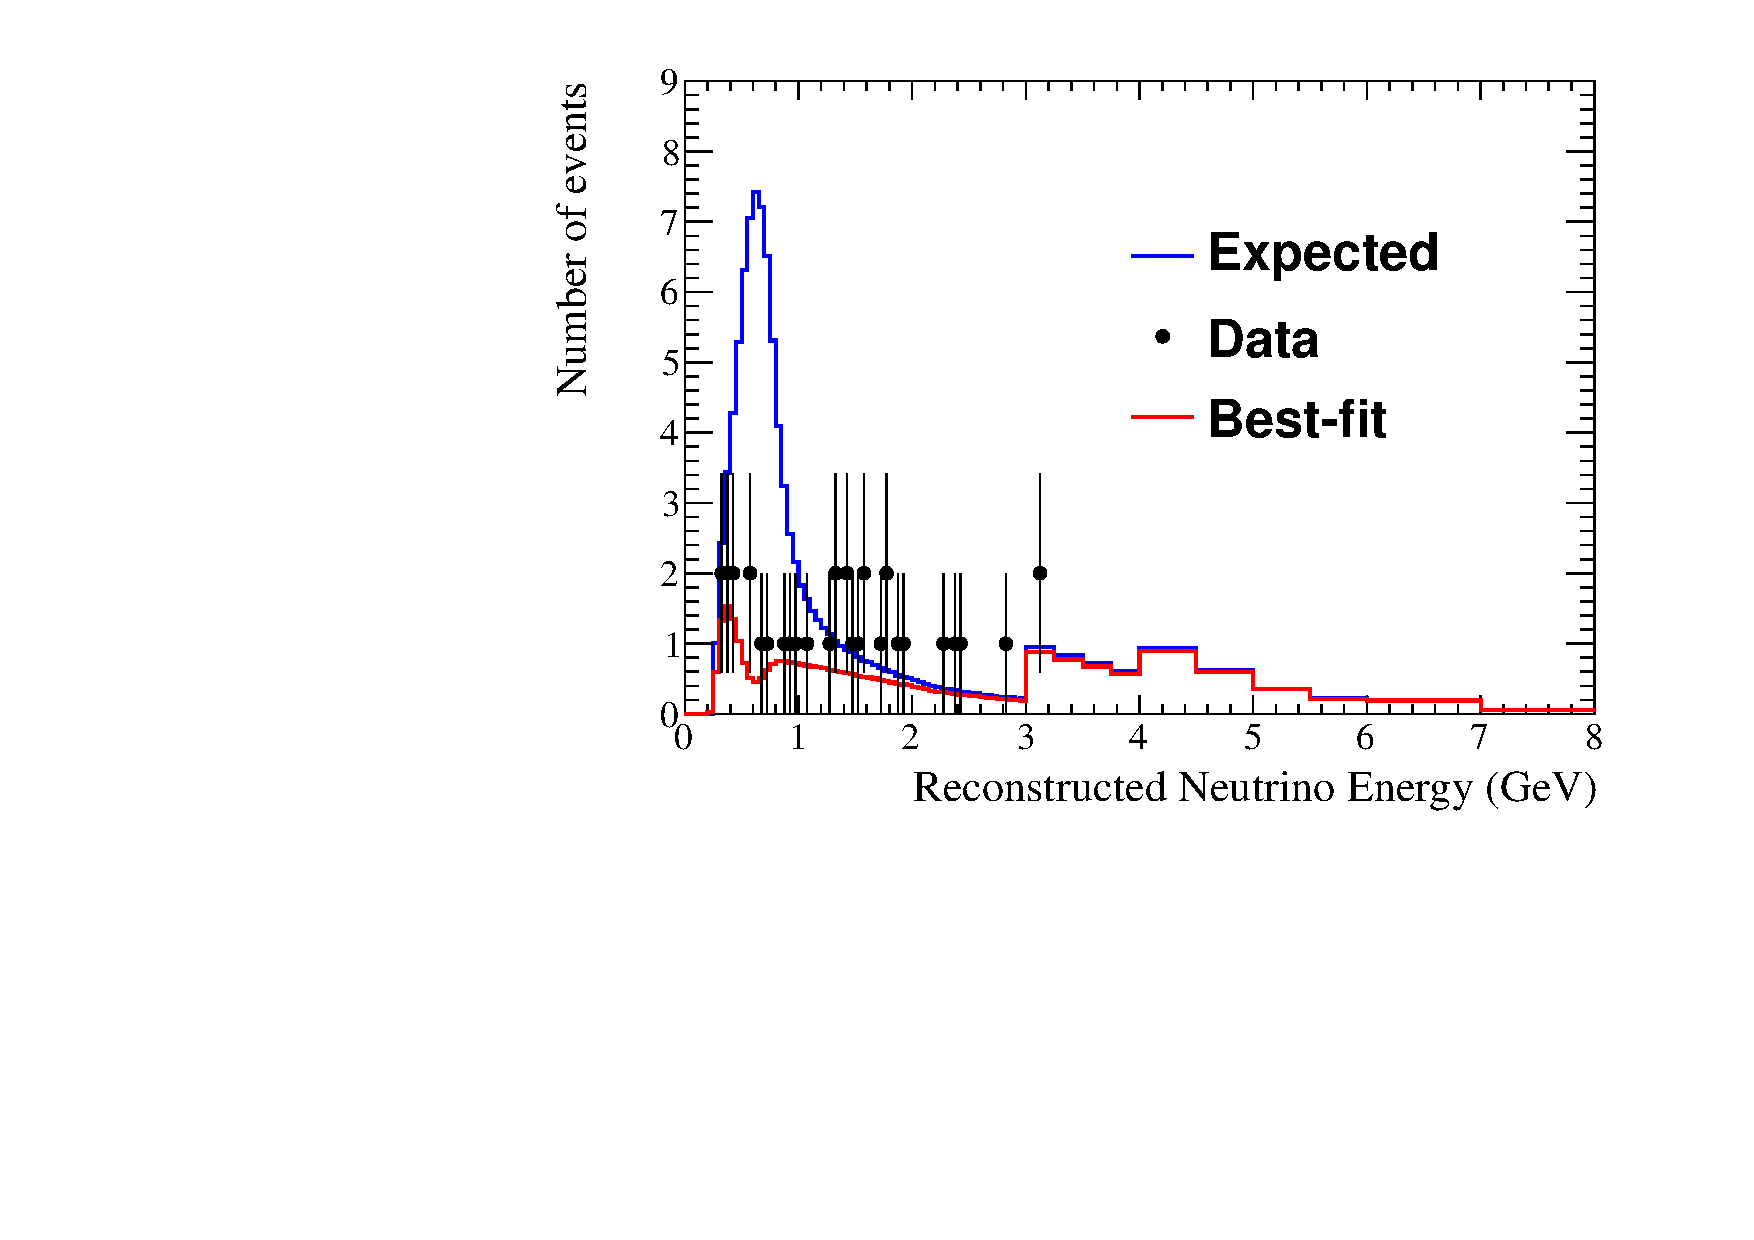
\includegraphics[width=0.9\textwidth]{joint_plots/data/bestfit_marg_sinsqth23Vsdcp_react_RHC1Rmu.pdf}
\caption{Muon-like, antineutrino mode}
\end{subfigure}
\begin{subfigure}[b]{0.49\textwidth}
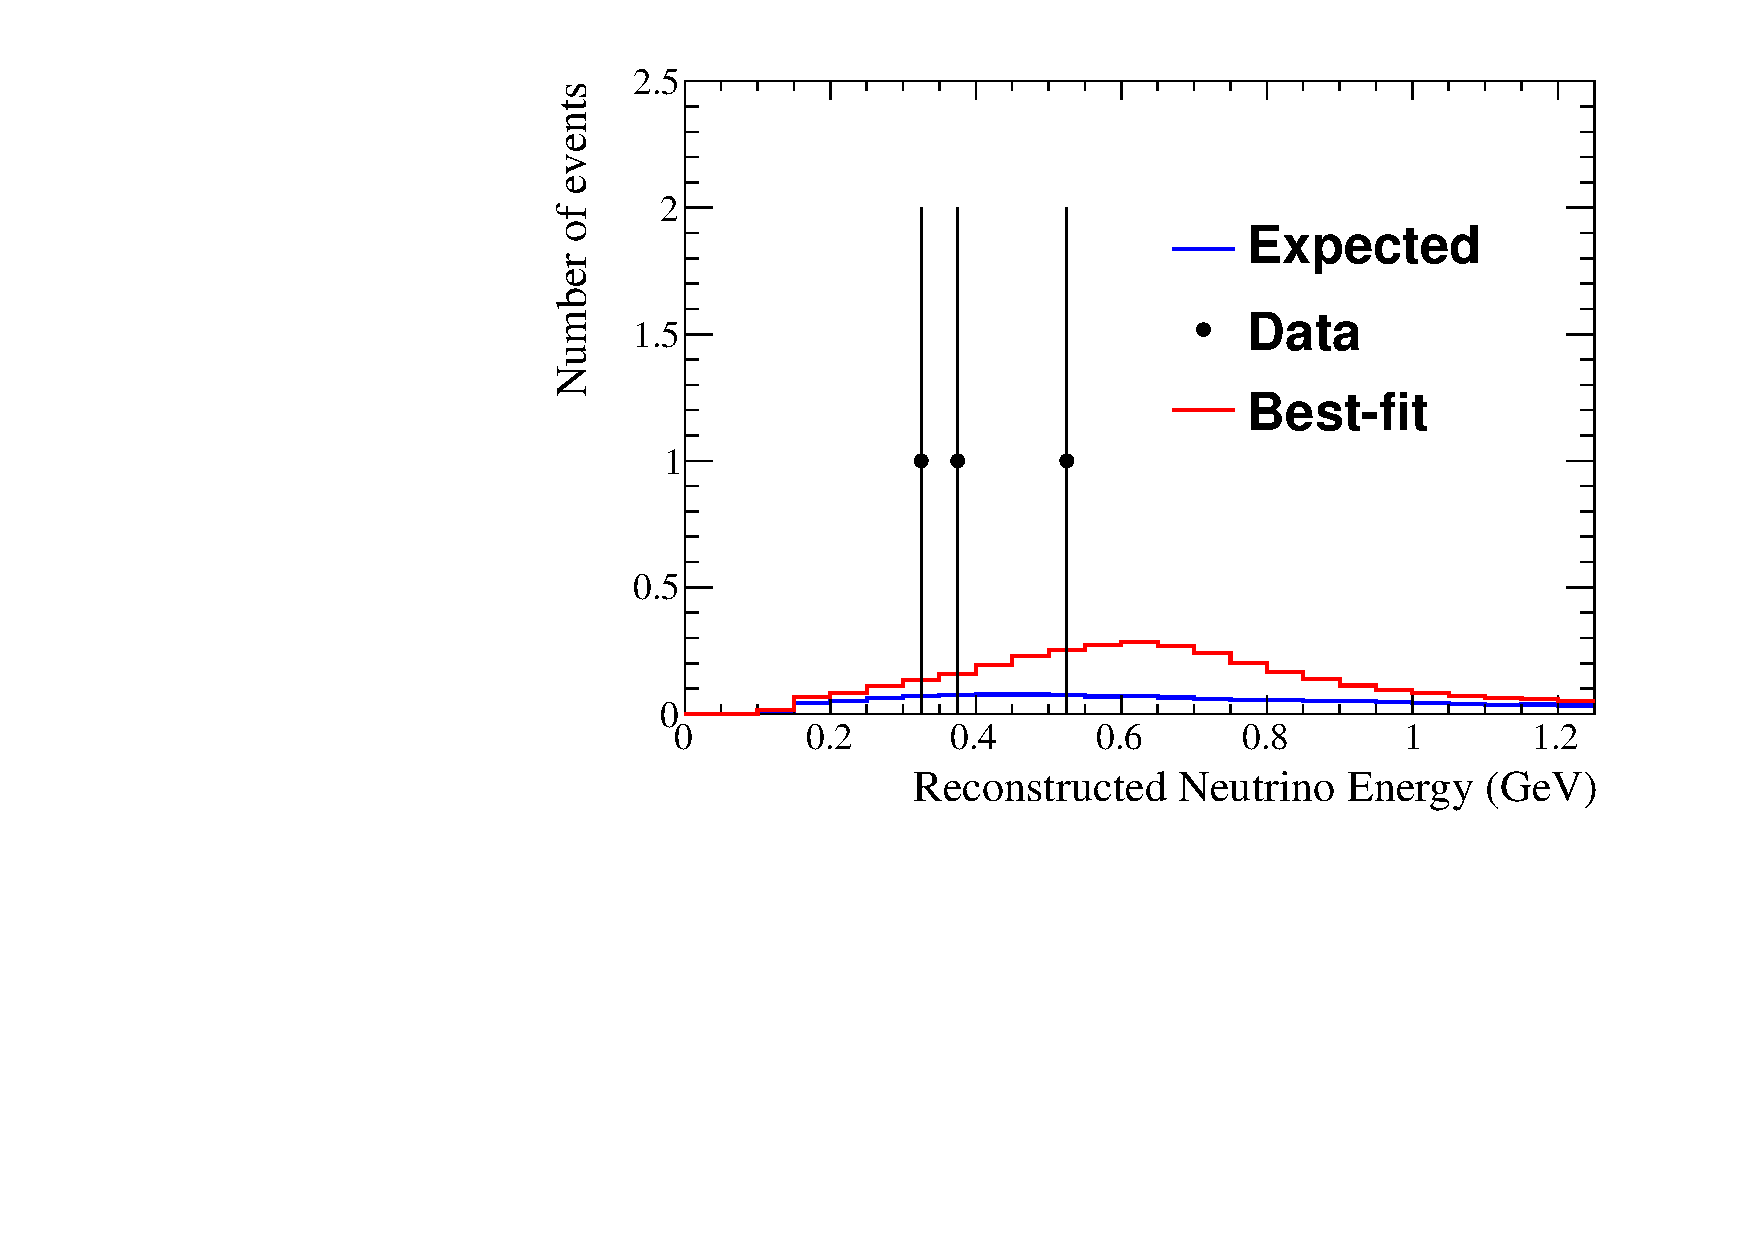
\includegraphics[width=0.9\textwidth]{joint_plots/data/bestfit_marg_sinsqth23Vsdcp_react_RHC1Re.pdf}
\caption{Electron-like, antineutrino mode}
\end{subfigure}
%\includegraphics[width=0.9\textwidth]{joint_plots/data/1rmu_ereco_tot_osc_notosc_bf.pdf}
%\includegraphics[width=0.9\textwidth]{joint_plots/data/rhc1rmu_ereco_tot_osc_notosc_bf.pdf}
%\includegraphics[width=0.9\textwidth]{joint_plots/data/1re_ereco_tot_osc_notosc_bf.pdf}
%\includegraphics[width=0.9\textwidth]{joint_plots/data/rhc1re_ereco_tot_osc_notosc_bf.pdf}
\caption {
%    \huge{TO UPDATE} % caption is already ok
%{\large{MEASURED BEST-FIT ERECO SPECTRA COMPARED TO DATA AND 
%PREDICTED UNOSCILLATED SPECTRA}}
The best-fit spectra as a function of the neutrino reconstructed energy
are shown for each selected sample
of the run 1-6 data set.
They correspond to the fit of 
$\sin^2 \theta_{23}$, $\delta_{CP}$ and mass hierarchy 
with reactor constraint
where all the nuisance parameters are marginalised. 
The method described in sec.~\ref{eq:bestfit_spectrum_marg} is used.
The best-fit distributions are compared with the 
predicted unoscillated spectrum (all the oscillation parameters are set to 0),
generated with the systematic parameters measured with the ND280 data 
shown in tab.~\ref{tab:banff_uncertainties_flux_fhc},
~\ref{tab:banff_uncertainties_flux_rhc},
~\ref{tab:banff_uncertainties_xsec}
and~\ref{tab:banff_uncertainties_skdetfsi}.
}
\label{fig:joint_spectra_bf}
\end{figure*}



% Goodness of fit

A goodness of test fit is performed by comparing data with the best fit spectra shown in \cref{fig:joint_spectra_bf}.
In order to determine how compatible the data is with our model 
the log likelihood is calculated for each sample as in \cref{eq:chisquare}
and the $\chi^2 / ndof$ is used to estimate the fit probability using the Poisson statistic, 
given the number of degrees of freedom equal to $ndof = N_{bins} - N_{free} (8-5 = 3)$,
where $N_{bins}$ is the number of template bins and $N_{free}$ is the number of free parameters in the fit.
The free parameters are $\sin^2 \theta_{23}$, $\delta_{CP}$ and the mass hierarchy in this case. 
In this analysis, a coarse binning scheme is used for the goodness of fit test as in previous analyses. 
This is used so that there are enough events in each bin to calculate p-values in the gaussian approximation. 
5 bins (0-0.4, 0.4-0.7, 0.7-1.0, 1.0-2.0 and 2.0-30.0 GeV) are used for the neutrino mode muon-like spectrum, 
1 bin is used for each of the muon-like antineutrino and electron-like spectra
in order to enter the gaussian regime, where the $\chi^2$ distribution is well defined.
The $\chi^2$ and resulting p-value for each spectrum is shown in Tab.~\ref{tab:goodness_of_fit}. 
We see for all the spectra, the data and best fit spectra are very compatible.

\begin{table}[htb]
\centering
\begin{tabular}{| c | c | c |}
\hline
 			& $\chi^2$ / ndf        		& p-value \\ \hline
MH fixed 		& 2.08917 / 6                  	& 0.84	\\ \hline
MH fitted 		& 2.08917 / 5                  	& 0.91	\\ \hline

\end{tabular}
\caption{
Goodness of fit for the 2-dimensional fit of $\sin^2 \theta_{23}$, $\delta_{CP}$ and mass hierarchy 
(both fitted and fixed)
where all the other parameters are marginalised. 
}
\label{tab:goodness_of_fit}
\end{table}

%\begin{table}[htb]
%\centering
%\begin{tabular}{| c | c | c | }
%\hline
%Sample		&  $\chi^2$ / ndf        			& p-value \\ \hline
%muon-like neutrino & 1.47751/ 2                  	&		0	\\ \hline
%muon-like antineutrino & 0.000378452 / 2   	&		0 \\	 \hline
%electron-like neutrino & 0.574525 / 2  		&		0 \\	\hline
%electron-like antineutrino & 0.0367553 / 2	&		0 \\		\hline
%\end{tabular}
%\caption{
%Goodness of fit for each sample spectrum from Sec.~\ref{sec:best_fit_spectra}. 
%}
%\label{tab:goodness_of_fit}
%\end{table}








%--------------------------------------------------------------------------------------
%
% Contours
%
%--------------------------------------------------------------------------------------

\subsection {2-dimensional confidence intervals}
\label{sec:results_bestfit}

The same 2-dimensional confidence intervals as in sec.~\ref{sec:sensi} are produced.
%In Fig.~\ref{fig:joint_chisq_t2krun14bf_2d_nh} and~\ref{fig:joint_chisq_t2krun14bf_2d_ih} the 2-dimensional $\chi^2$ distributions 
%obtained by the fit of the Run 1-6 data set are shown for both normal and inverted hierarchy.
In Fig.~\ref{fig:joint_sensi_t2krun14bf_2d} the corresponding 2-dimensional contours produced
with the Run 1-6 data set are shown drawing the normal and inverted hierarchy contours independently,
i.e. each contour is produced with respect to the global minimum under that hierarchy hypothesis.
In Fig.~\ref{fig:joint_sensi_t2krun14bf_2d_glob} both normal and inverted hierarchy contours
are produced with respect to the same global minimum, i.e. the normal hierarchy hypothesis.

As already explained in \cref{sec:cl_mh}, ``global" and ``independent" contours correspond
respectively to the least and most conservative approach.

As in 1-dimensional analysis results,
looking at contours of $\sin^2 \theta_{13}$ Vs $\delta_{CP}$ with T2K only data, 
in Fig~\ref{fig:ss13_dcp_t2k_only_data_fit}, it is clear that the reactor measurements are 
in agreement with the T2K data at $1\sigma$ level if $\delta_{CP} \sim - \frac{\pi}{2}$. The tension 
between the $\sin^2 \theta_{13}$ reactor constraint and the T2K data constraint is clear at 
$\sim \frac{+\pi}{2}$ where the T2K data prefer a lager mixing angle with both hierarchy hypotheses.
This is the cause of the closed 90\% contour in Fig~\ref{fig:ss13_dcp_with_reactor_data_fit} which is also in good agreement with the 1D $\delta_{CP}$ fit in Fig.\ref{fig:dcp_fit_with_reactor_data}. This effect is much greater for the inverted hierarchy fits and thus leads to a much tighter constraint on $\delta_{CP}$. 
As a result, we see that all $\delta_{CP}$ constraints in 
Fig.~\ref{fig:ss13_dcp_with_reactor_data_fit},~\ref{fig:dmsq_dcp_with_reactor_data_fit},~\ref{fig:ss23_dcp_with_reactor_data_fit} 
are tighter for the inverted hierarchy hypothesis than for the normal.
Fig~\ref{fig:dmsq_dcp_with_reactor_data_fit} also shows a slight anti-correlation between $\delta_{CP}$ 
and $\Delta m^2_{32}$ in the normal hierarchy fit and a correlation in the inverted most likely coming 
from the fact that $\Delta m^2_{32}$ and $cos(\delta_{CP})$ have similar effects on the shape of the appearance spectra. 
In Fig~\ref{fig:ss23_dcp_with_reactor_data_fit} we see correlation where the constraint on $\delta_{CP}$ is narrower 
for smaller values of $\sin^2 \theta_{23}$ as they both appear in the appearance term. 
In Fig~\ref{fig:ss23_dmsq_with_reactor_data_fit} we see that $\sin^2 \theta_{23}$ and $\Delta m^2_{32}$ 
are not very correlated however the inverted hierarchy contour is shifted down in $\Delta m^2_{32}$ 
with respect to the normal hierarchy contour. 
This effect is due to the correlation between $\Delta m^2_{32}$ and the mass hierarchy shown in Fig.~\ref{fig:mass_hierarchy_MC_shift}. 
Indeed the inverted hierarchy hypothesis produces an event migration toward higher energy 
which is balanced in the fit by a lower fit value of $\Delta m^2_{13}$ with respect to the normal hierarchy case.

%This effect is likely due to the correlations between the hierarchy and $\delta_{CP}$ which we see in Fig.~\ref{fig:ss13_dcp_with_reactor_data_fit}, where inverted hierarchy fit excludes $cos(\delta_{CP})=-1$ to a greater significance than the normal hierarchy fit, and $\Delta m^2_{32}$ and $\delta_{CP}$ in Fig.~\ref{fig:dmsq_dcp_with_reactor_data_fit}. 

The \emph{constant} $\Delta \chi^2$ contours with respect to the global minimum in Fig.~\ref{fig:joint_sensi_t2krun14bf_2d_glob} show similar trends. 
As the normal hierarchy was preferred in all fits, the normal hierarchy contours are identical to those in Fig.~\ref{fig:joint_sensi_t2krun14bf_2d}. 
The inverted hierarchy contours are noticeably tighter in all cases. 
In Fig~\ref{fig:ss13_dcp_t2k_only_data_fit_global} we see that there is a closed $\Delta \chi^2=4.61$ contour, 
and in all others the $\Delta \chi^2=4.61$ contour is of similar size to the $\Delta \chi^2=2.3$ contour for the normal hierarchy. 

%\begin{figure*}[htb]
%\center
%
\includegraphics[width=0.9\textwidth]{./images/missing_plot-eps-converted-to.pdf}
%
\includegraphics[width=0.9\textwidth]{./images/missing_plot-eps-converted-to.pdf}
%
\includegraphics[width=0.9\textwidth]{./images/missing_plot-eps-converted-to.pdf}
%\caption{
%{\large{MEASURED 2D CHISQ DISTRIBUTIONS FOR NORMAL HIERARCHY}}
%$\chi^2$ distributions measured  
%with the full run 1-6 data set.
%Normal hierarchy is shown. 
%From top left to bottom right the following combinations of oscillation parameters are shown:
%$\sin^2 \theta_{13}$ Vs $\delta_{CP}$ with T2K data only,
%$\sin^2 \theta_{13}$ Vs $\delta_{CP}$ with reactor constraint
%and
%$\sin^2 \theta_{23}$ Vs $\Delta m^2_{32}$ ($\Delta m^2_{13}$)
%with reactor constraint.
%All the oscillation parameters which are not parameters of interest
%are marginalised using the prior distributions shown in tab.~\ref{tab:osc_params_joint}.
%The $\chi^2$ distribution of $\sin^2 \theta_{13}$ Vs $\delta_{CP}$ without reactor constraint
%is compared with the measurement performed by the reactor experiments, 
%$\sin^2 \theta_{13} = 0.0219 \pm 0.0012 $
%\cite{pdg_2014},
%shown by the yellow bar.
%}
%\label{fig:joint_chisq_t2krun14bf_2d_nh}
%\end{figure*}
%
%\begin{figure*}[htb]
%\center
%
\includegraphics[width=0.9\textwidth]{./images/missing_plot-eps-converted-to.pdf}
%
\includegraphics[width=0.9\textwidth]{./images/missing_plot-eps-converted-to.pdf}
%
\includegraphics[width=0.9\textwidth]{./images/missing_plot-eps-converted-to.pdf}
%\caption{
%{\large{MEASURED 2D CHISQ DISTRIBUTIONS FOR INVERTED HIERARCHY}}
%$\chi^2$ distributions measured  
%with the full run 1-6 data set.
%Inverted hierarchy is shown. 
%From top left to bottom right the following combinations of oscillation parameters are shown:
%$\sin^2 \theta_{13}$ Vs $\delta_{CP}$ with T2K data only,
%$\sin^2 \theta_{13}$ Vs $\delta_{CP}$ with reactor constraint
%and
%$\sin^2 \theta_{23}$ Vs $\Delta m^2_{32}$ ($\Delta m^2_{13}$)
%with reactor constraint.
%All the oscillation parameters which are not parameters of interest
%are marginalised using the prior distributions shown in tab.~\ref{tab:osc_params_joint}.
%The $\chi^2$ distribution of $\sin^2 \theta_{13}$ Vs $\delta_{CP}$ without reactor constraint
%is compared with the measurement performed by the reactor experiments, 
%$\sin^2 \theta_{13} = 0.0219 \pm 0.0012 $
%\cite{pdg_2014},
%shown by the yellow bar.
%}
%\label{fig:joint_chisq_t2krun14bf_2d_ih}
%\end{figure*}

\begin{figure*}[htb]
\center
\begin{subfigure}[b]{0.49\textwidth}
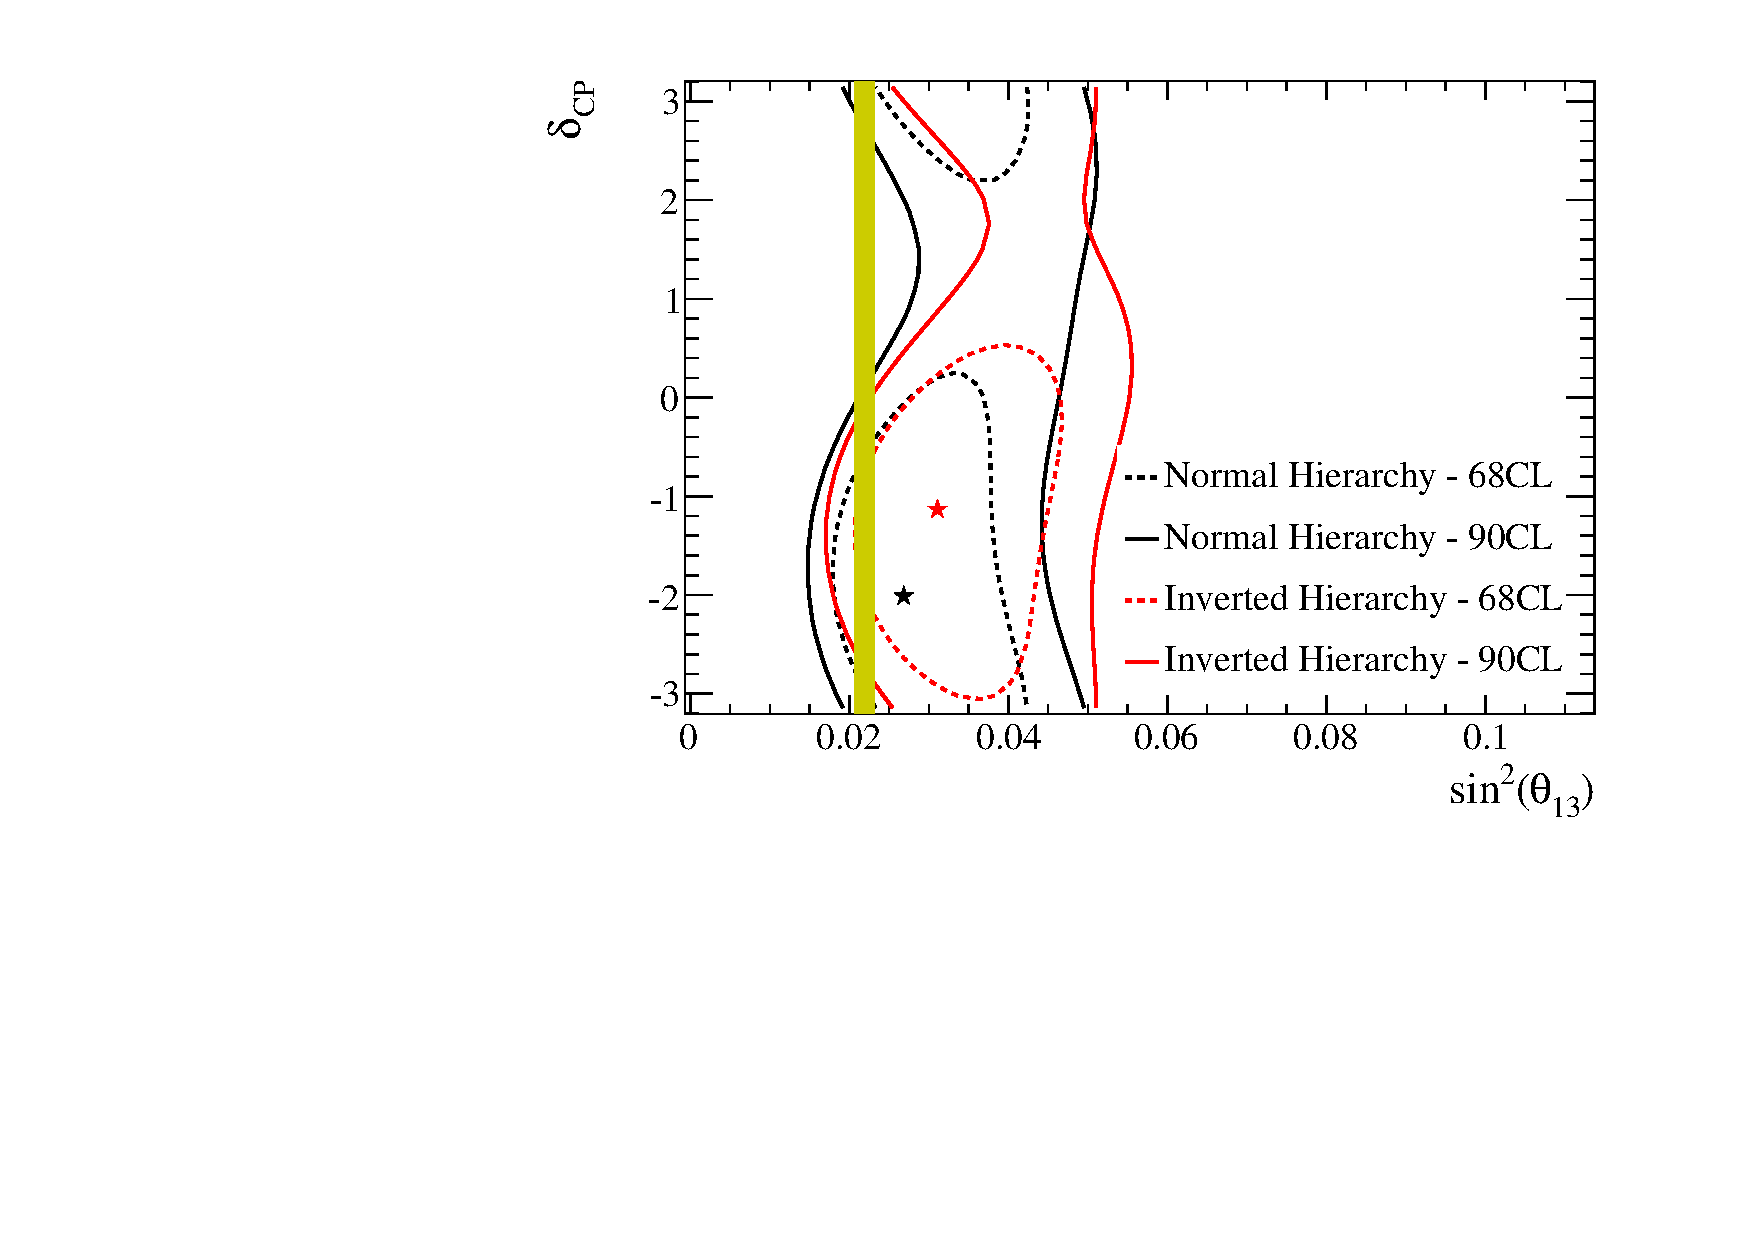
\includegraphics[width=0.9\textwidth]{joint_plots/data_contours/sinsqth13Vsdcp_t2konly_data_constdchisq.pdf}
\caption{$\sin^2 \theta_{13}$ Vs $\delta_{CP}$ with T2K data only}
\label{fig:ss13_dcp_t2k_only_data_fit}
\end{subfigure}
\begin{subfigure}[b]{0.49\textwidth}
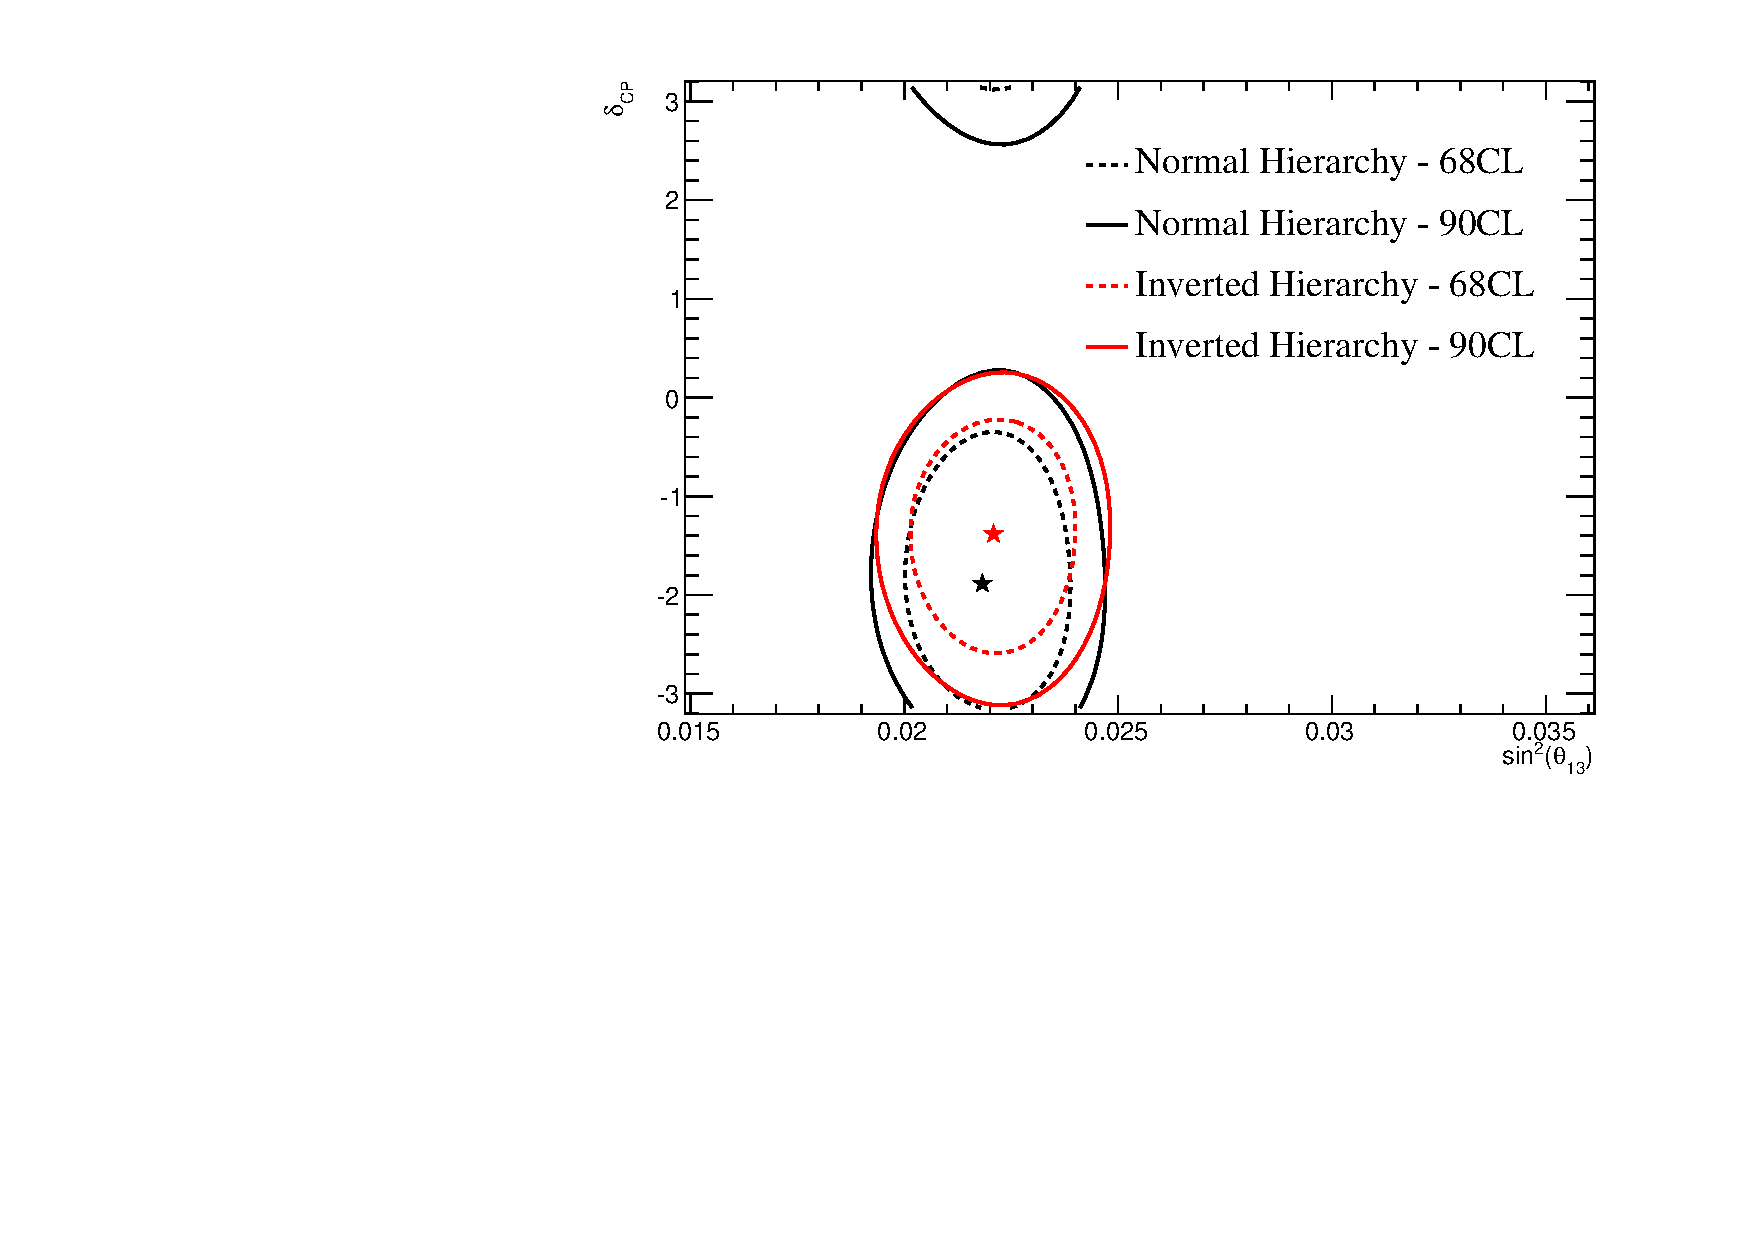
\includegraphics[width=0.9\textwidth]{joint_plots/data_contours/sinsqth13Vsdcp_react_data_constdchisq.pdf}
\caption{$\sin^2 \theta_{13}$ Vs $\delta_{CP}$ with reactor constraint}
\label{fig:ss13_dcp_with_reactor_data_fit}
\end{subfigure}
\begin{subfigure}[b]{0.49\textwidth}
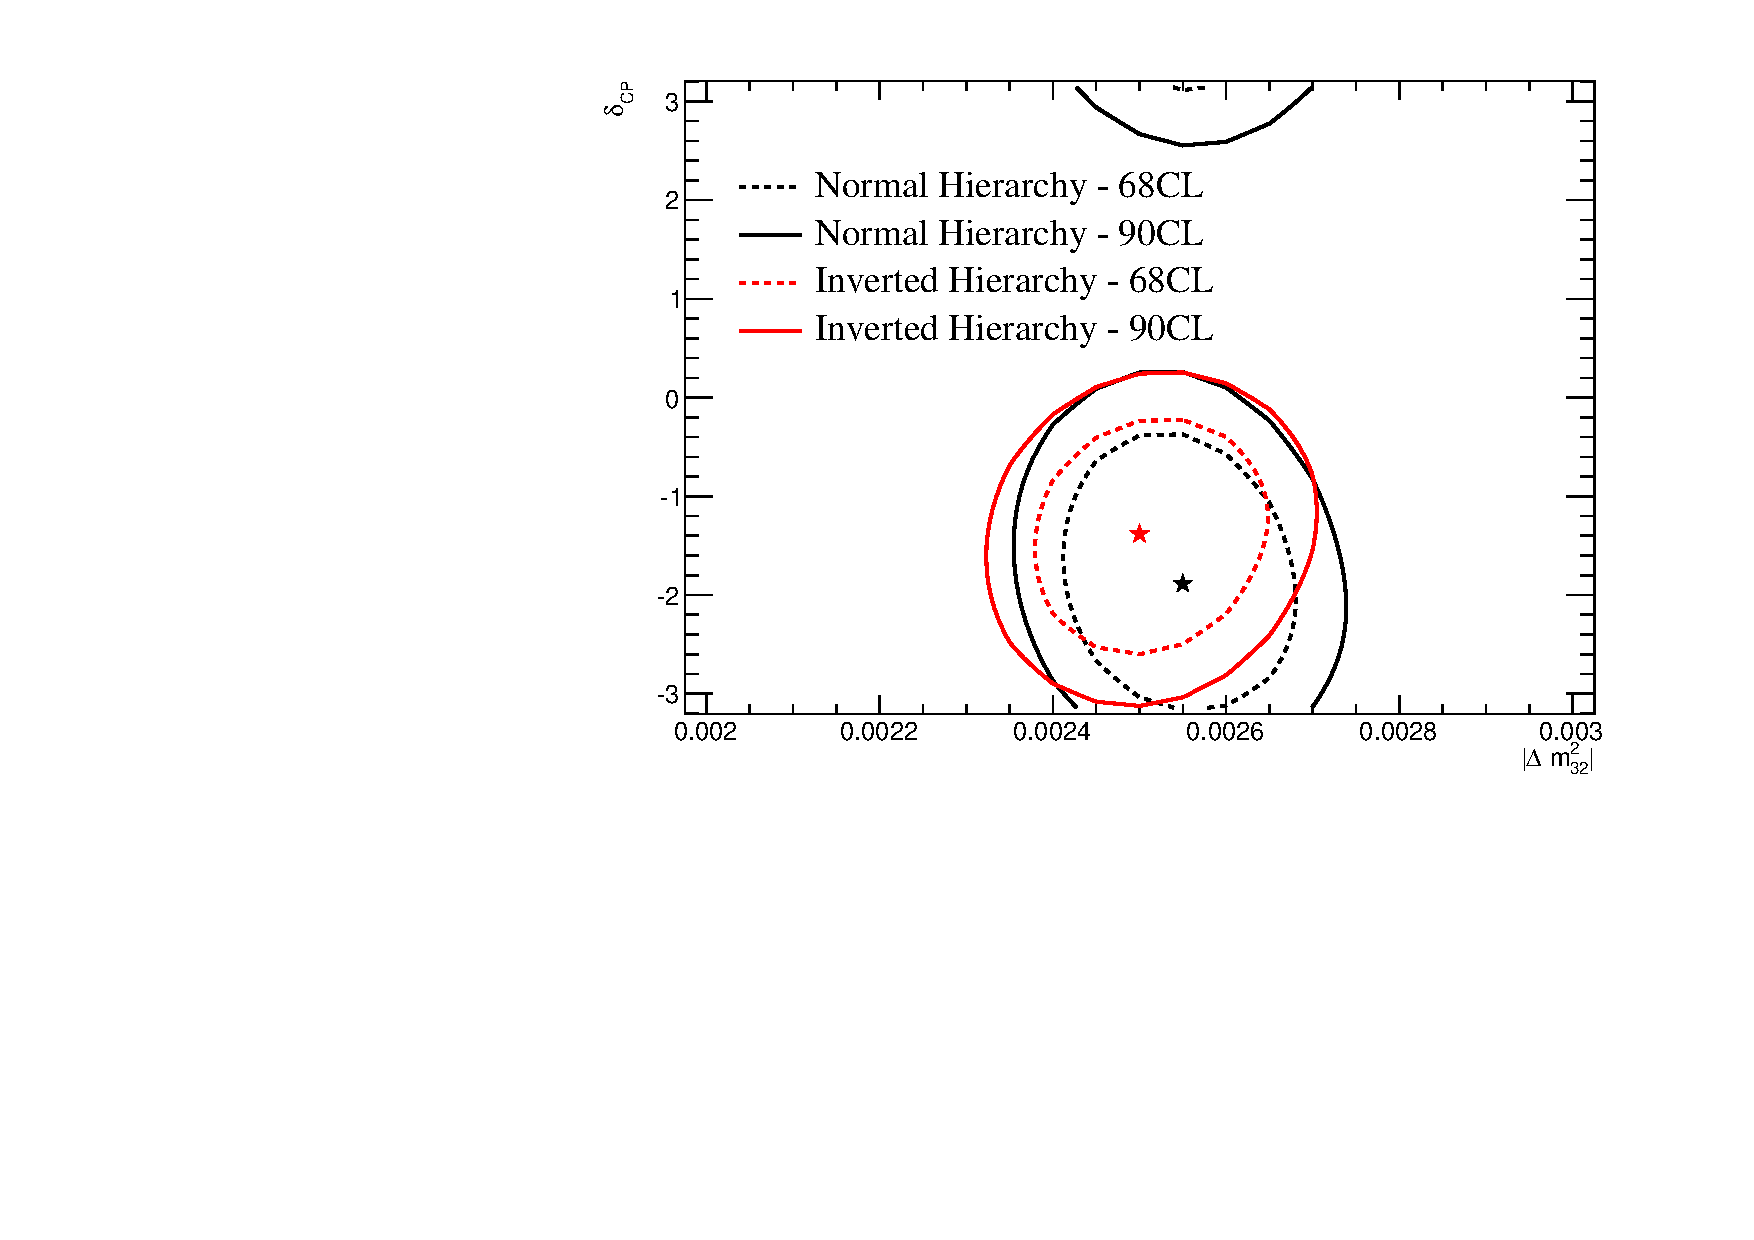
\includegraphics[width=0.9\textwidth]{joint_plots/data_contours/dmsqVsdcp_react_data_constdchisq.pdf}
\caption{$\Delta m^2_{32}$ ($\Delta m^2_{13}$) Vs $\delta_{CP}$ with reactor constraint}
\label{fig:dmsq_dcp_with_reactor_data_fit}
\end{subfigure}
\begin{subfigure}[b]{0.49\textwidth}
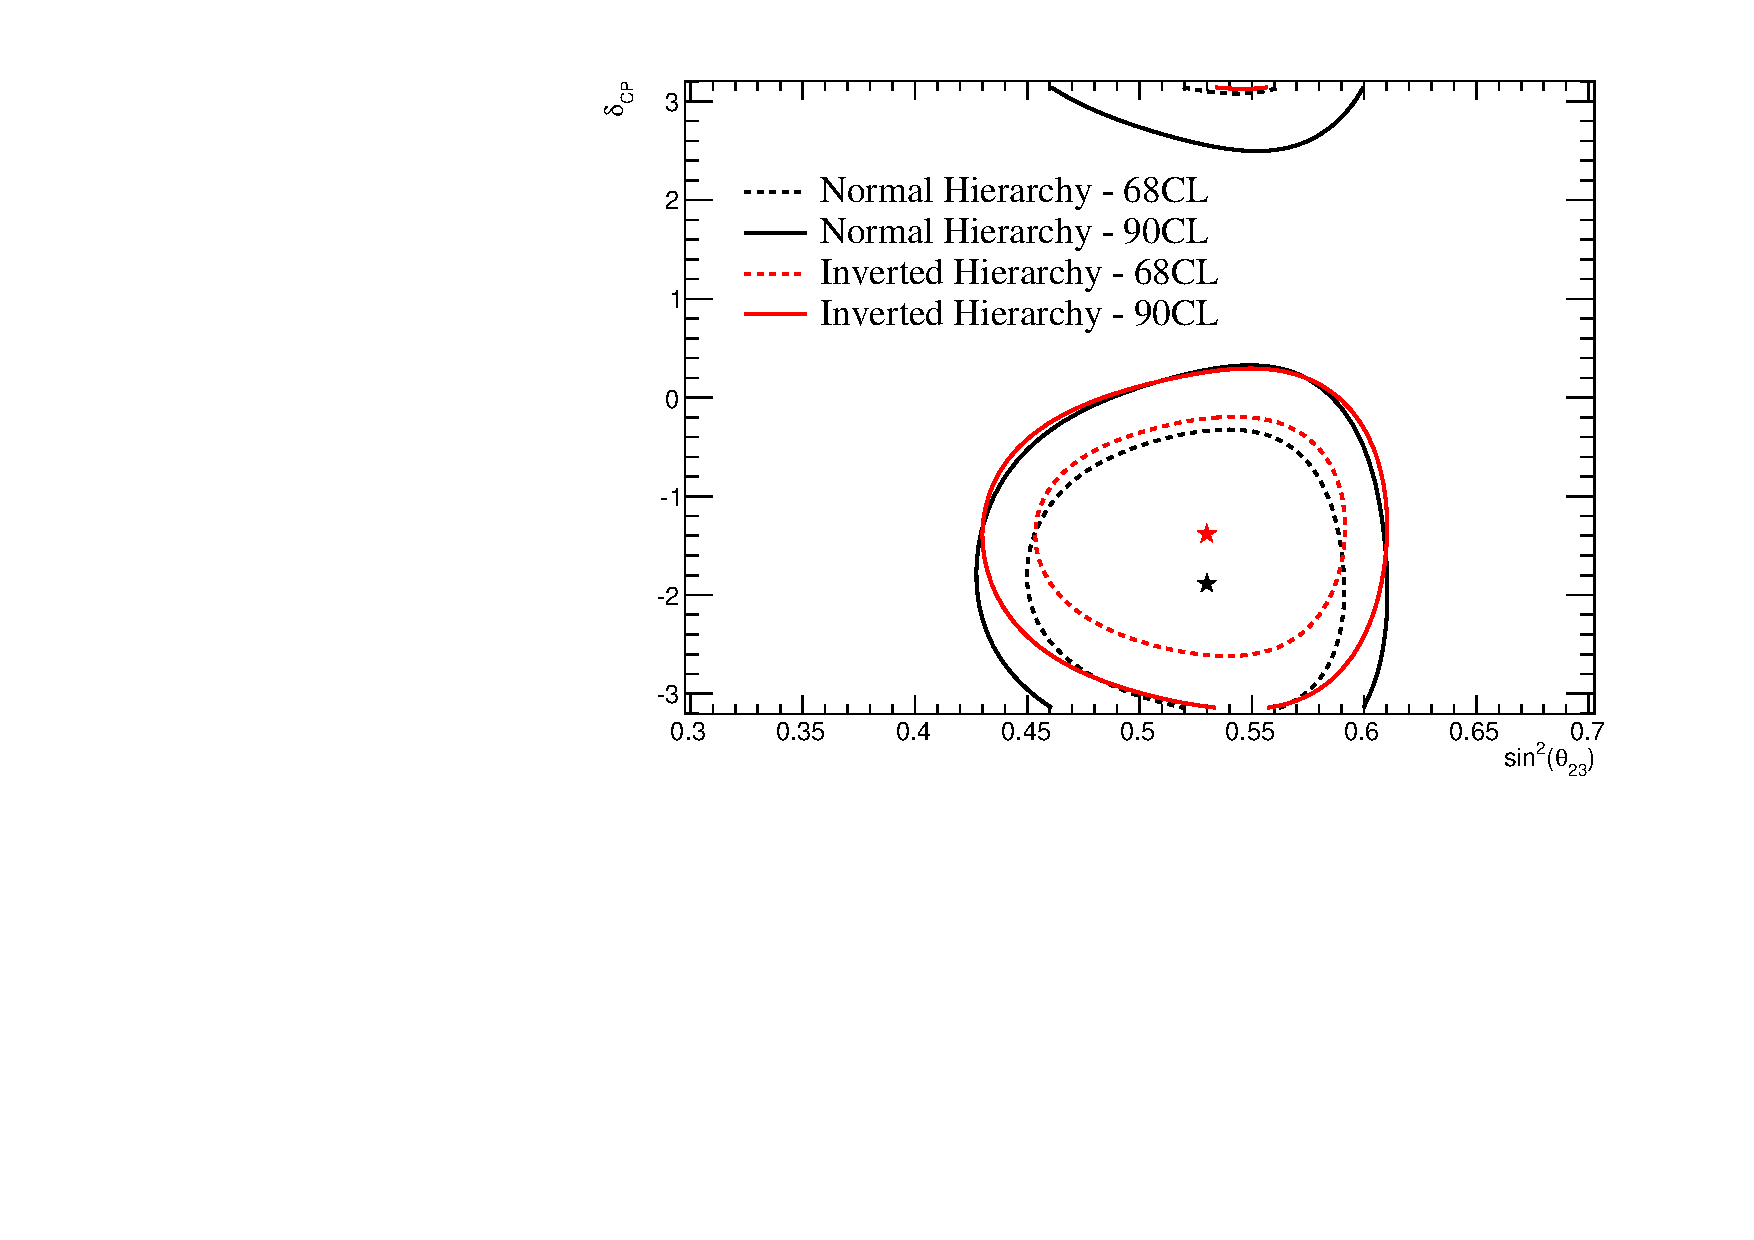
\includegraphics[width=0.9\textwidth]{joint_plots/data_contours/sinsqth23Vsdcp_react_data_constdchisq.pdf}
\caption{$\sin^2 \theta_{23}$ Vs $\delta_{CP}$ with reactor constraint}
\label{fig:ss23_dcp_with_reactor_data_fit}
\end{subfigure}
\begin{subfigure}[b]{0.49\textwidth}
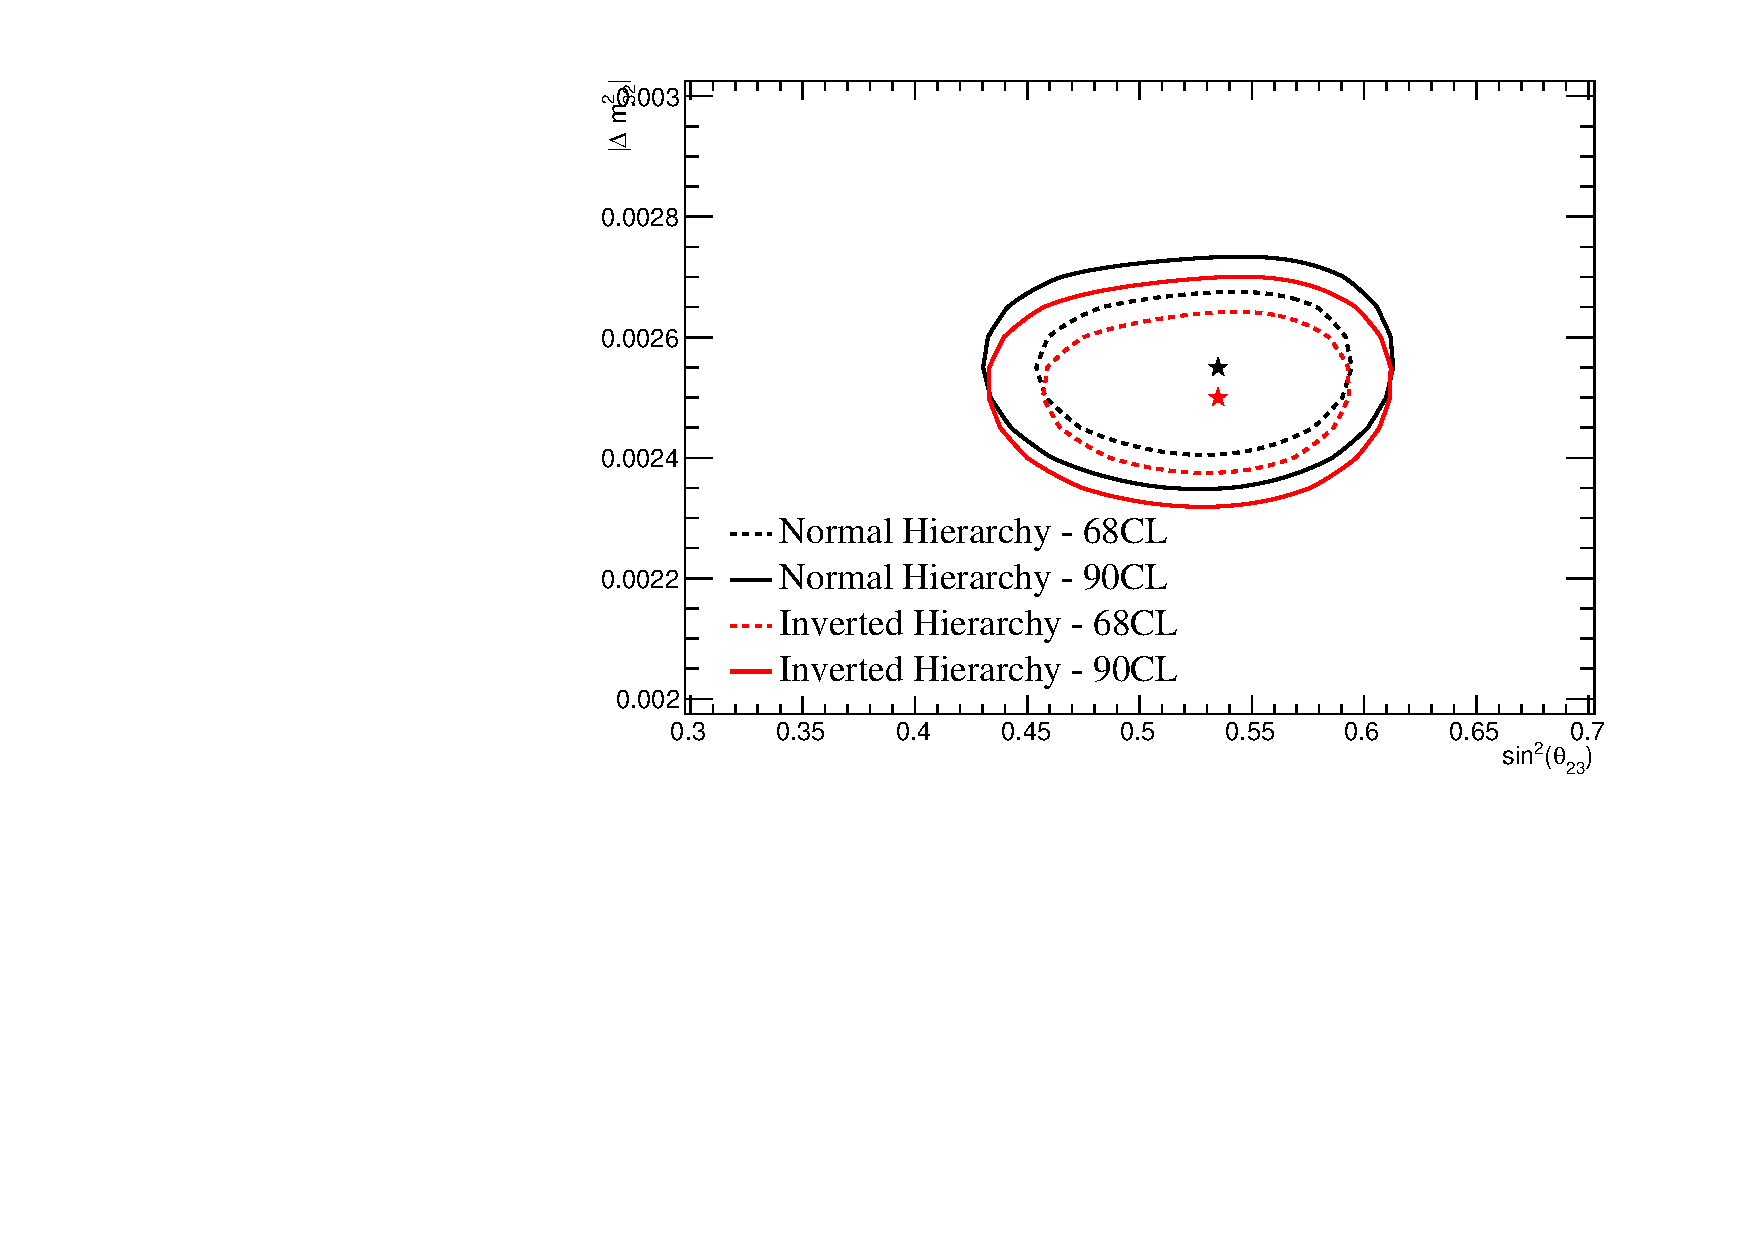
\includegraphics[width=0.9\textwidth]{joint_plots/data_contours/sinsqth23Vsdmsq_react_data_constdchisq.pdf}
\caption{$\sin^2 \theta_{23}$ Vs $\Delta m^2_{32}$ ($\Delta m^2_{13}$)
with reactor constraint}
\label{fig:ss23_dmsq_with_reactor_data_fit}
\end{subfigure}

%
\includegraphics[width=0.9\textwidth]{./images/missing_plot-eps-converted-to.pdf}
\caption{
%{\large{MEASURED 2D CONTOURS}}
Measured confidence intervals with the full run 1-6 data set.
Both normal (black) and inverted (red) hierarchies are shown. 
Both 68\% (dashed line) and 90\% CL (solid line) are shown.
Confidence intervals are produced using the \emph{constant} $\Delta \chi^2$ method. % (see app.~\ref{app:method_cl}).
Contours for normal (black) and inverted (red) hierarchy are computed independently
with respect to the global minimum of each hierarchy (star).
All the oscillation parameters which are not parameters of interest
are marginalised using the prior distributions shown in tab.~\ref{tab:osc_params_joint_priors}.
The measured contour of $\sin^2 \theta_{13}$ Vs $\delta_{CP}$ without reactor constraint, in Fig~\ref{fig:ss13_dcp_t2k_only_data_fit} is compared with the measurement by reactor experiments, 
$\sin^2 \theta_{13} = 0.0219 \pm 0.0012 $
\cite{pdg_2014},
shown by the yellow bar.
}
\label{fig:joint_sensi_t2krun14bf_2d}
\end{figure*}


\begin{figure*}[htb]
\center
\begin{subfigure}[b]{0.49\textwidth}
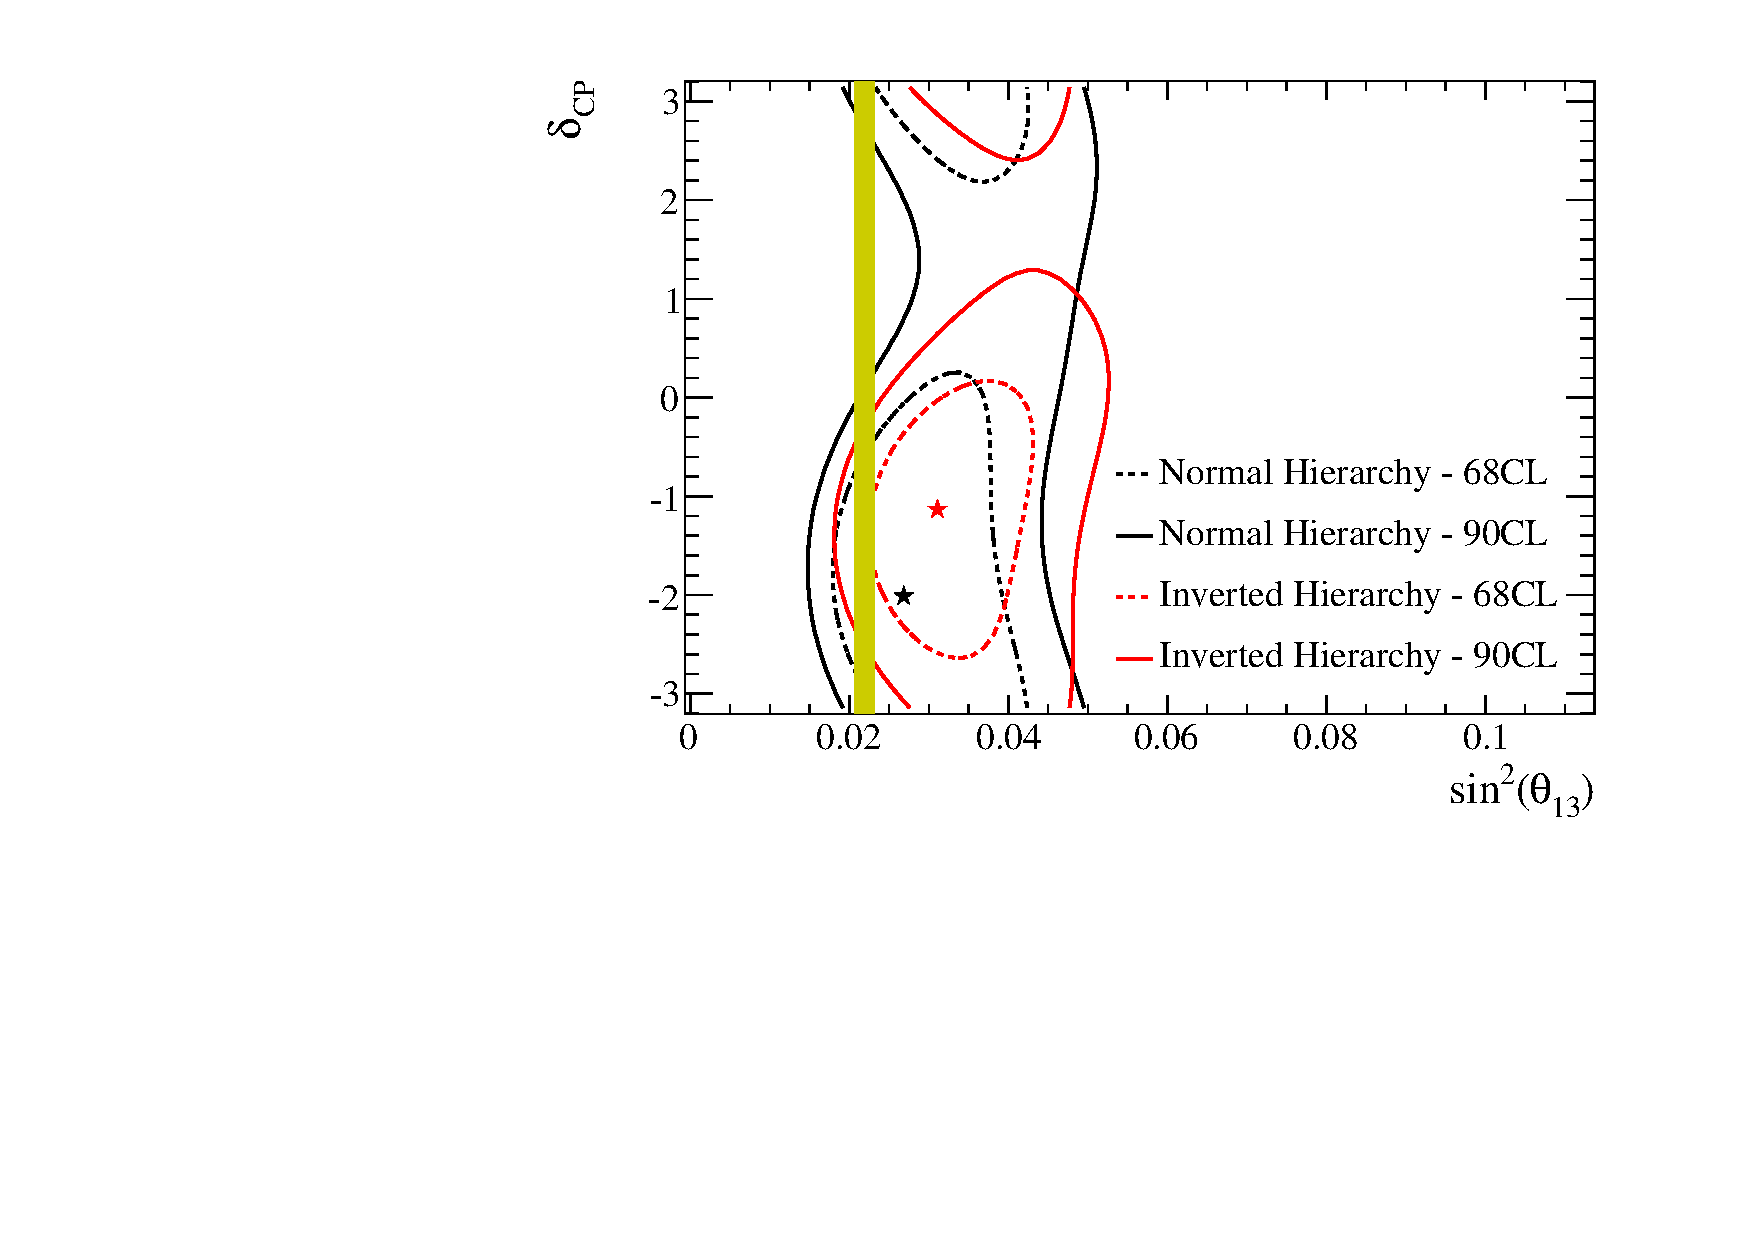
\includegraphics[width=0.9\textwidth]{joint_plots/data_contours/sinsqth13Vsdcp_t2konly_data_constdchisq_glob.pdf}
\caption{$\sin^2 \theta_{13}$ Vs $\delta_{CP}$ with T2K data only}
\label{fig:ss13_dcp_t2k_only_data_fit_global}
\end{subfigure}
\begin{subfigure}[b]{0.49\textwidth}
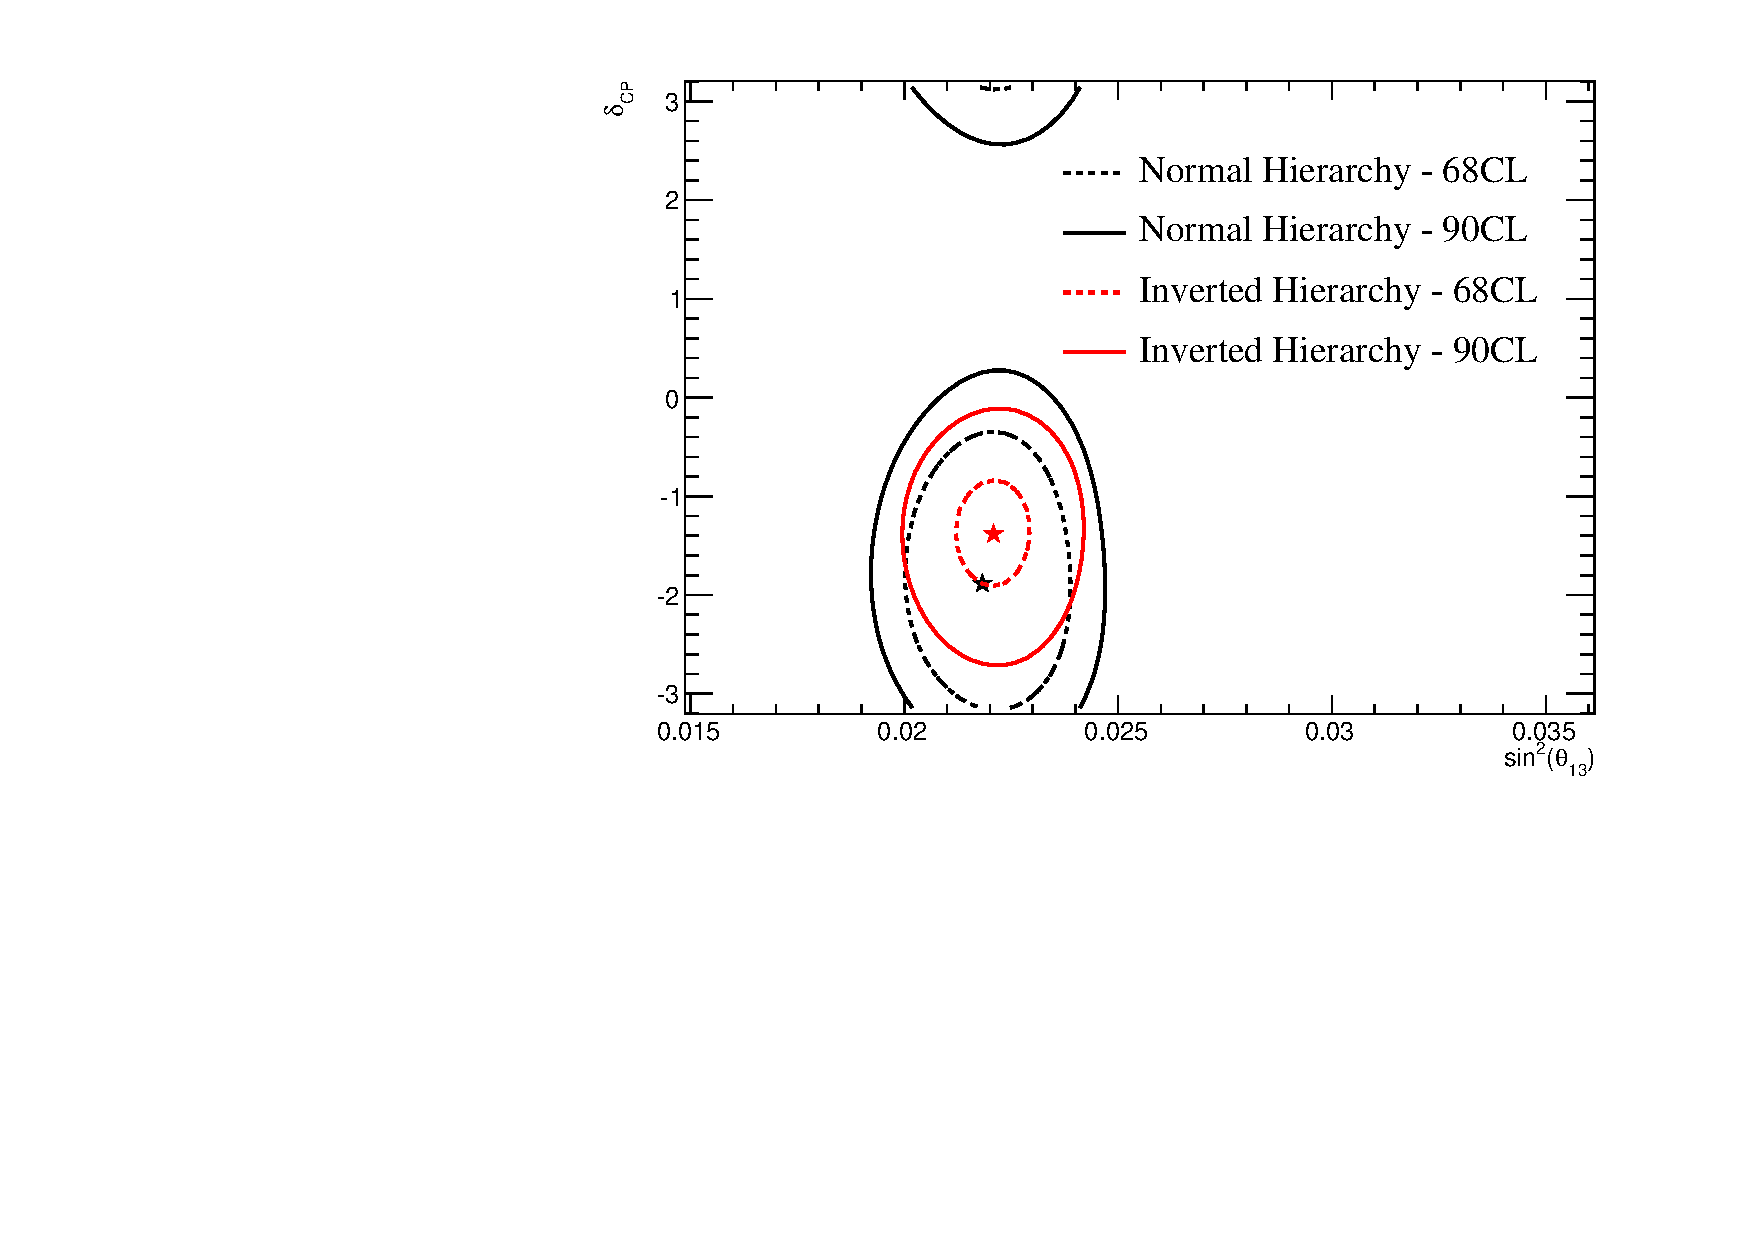
\includegraphics[width=0.9\textwidth]{joint_plots/data_contours/sinsqth13Vsdcp_react_data_constdchisq_glob.pdf}
\caption{$\sin^2 \theta_{13}$ Vs $\delta_{CP}$ with reactor constraint}
\end{subfigure}
\begin{subfigure}[b]{0.49\textwidth}
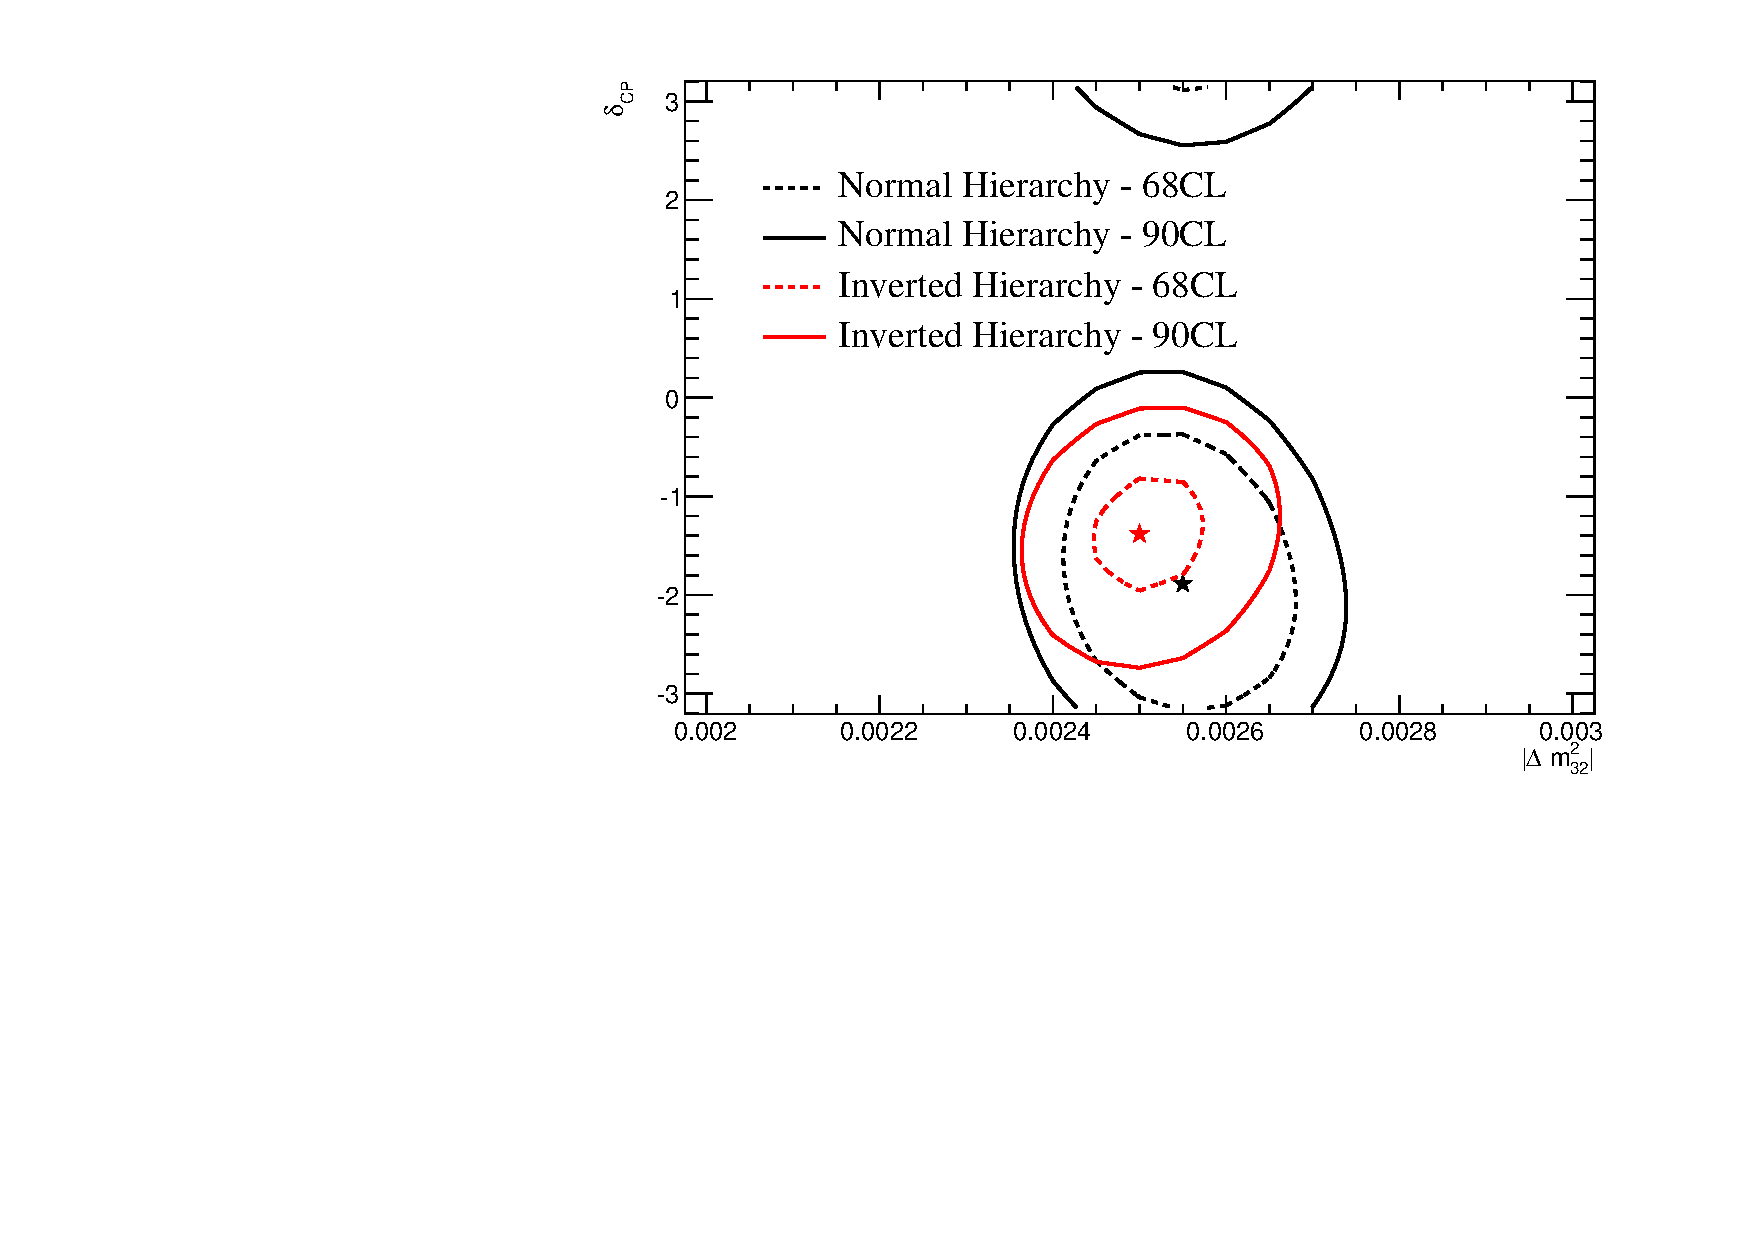
\includegraphics[width=0.9\textwidth]{joint_plots/data_contours/dmsqVsdcp_react_data_constdchisq_glob.pdf}
\caption{$\Delta m^2_{32}$ ($\Delta m^2_{13}$) Vs $\delta_{CP}$ with reactor constraint}
\end{subfigure}
\begin{subfigure}[b]{0.49\textwidth}
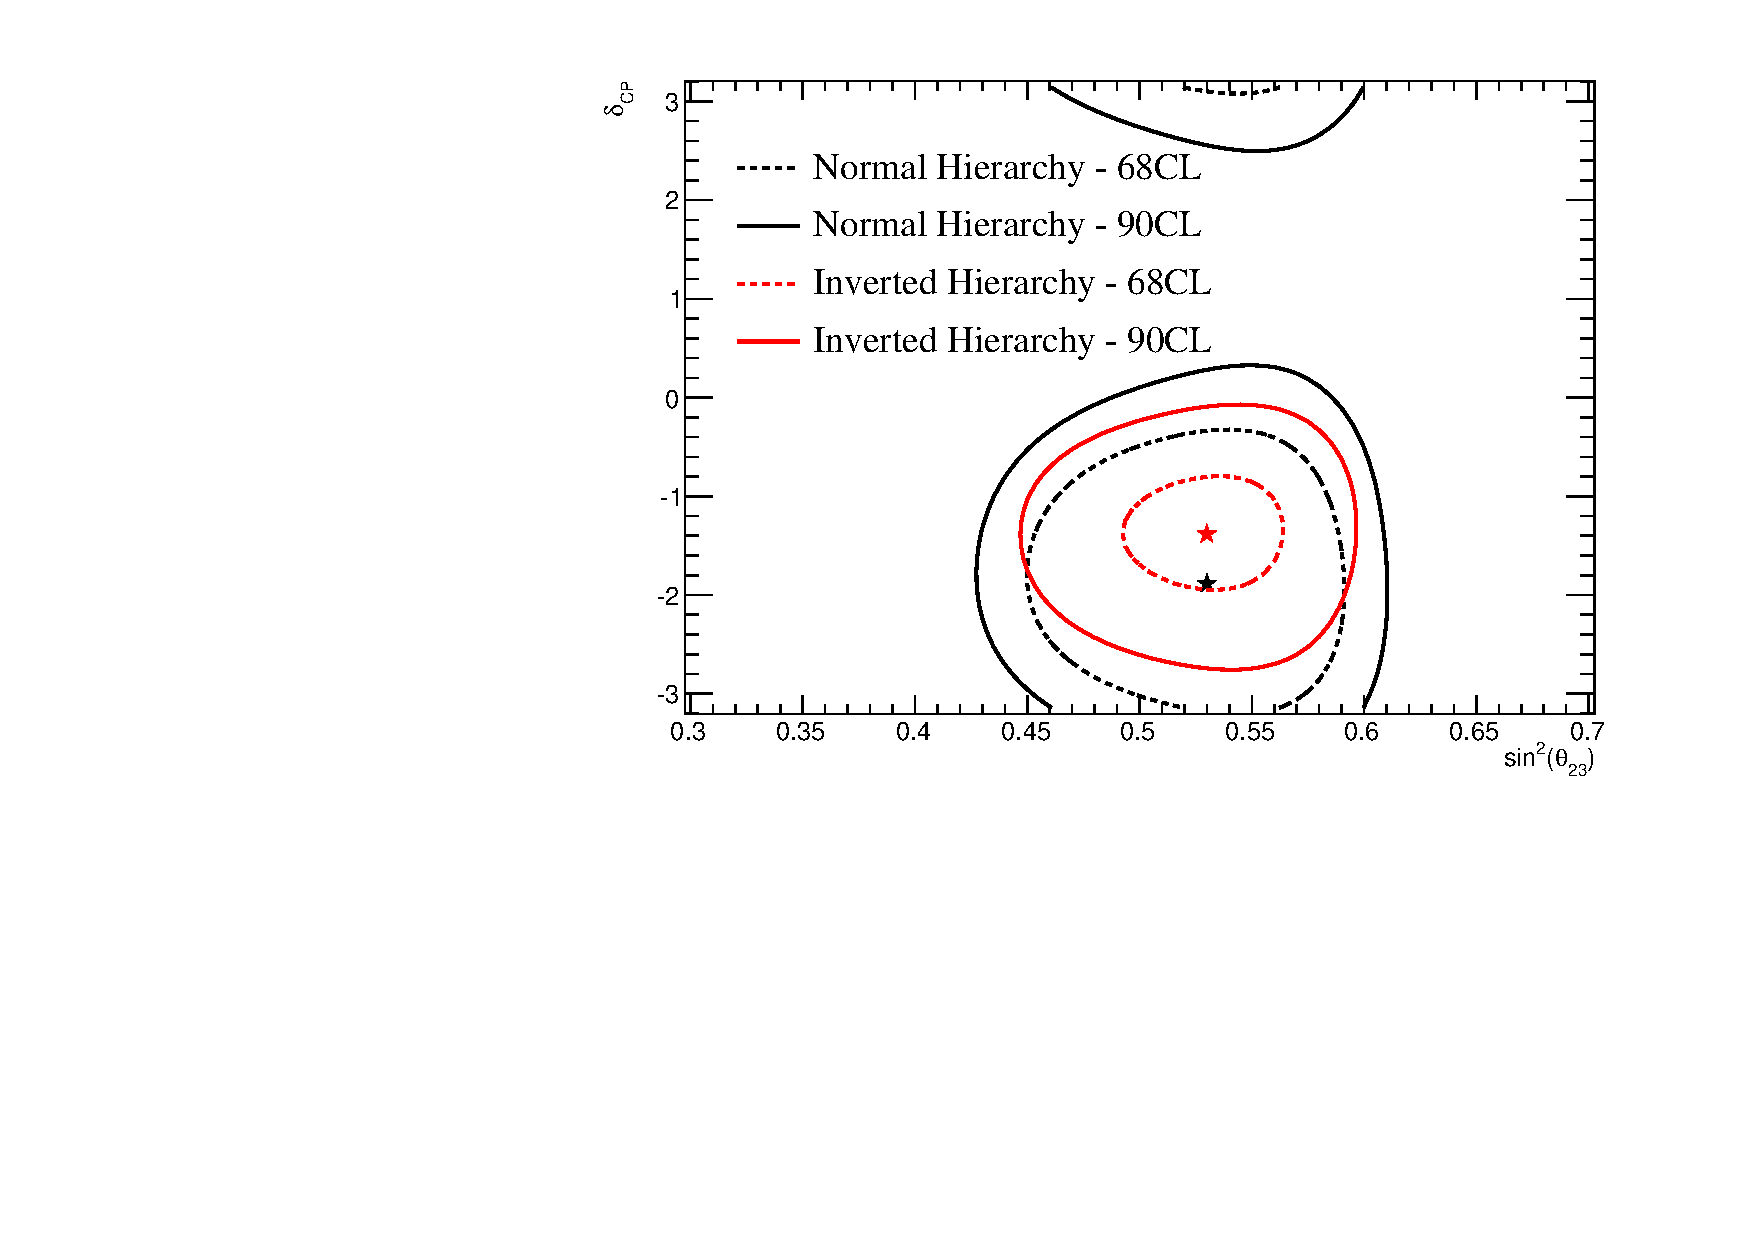
\includegraphics[width=0.9\textwidth]{joint_plots/data_contours/sinsqth23Vsdcp_react_data_constdchisq_glob.pdf}
\caption{$\sin^2 \theta_{23}$ Vs $\delta_{CP}$ with reactor constraint}
\end{subfigure}
\begin{subfigure}[b]{0.49\textwidth}
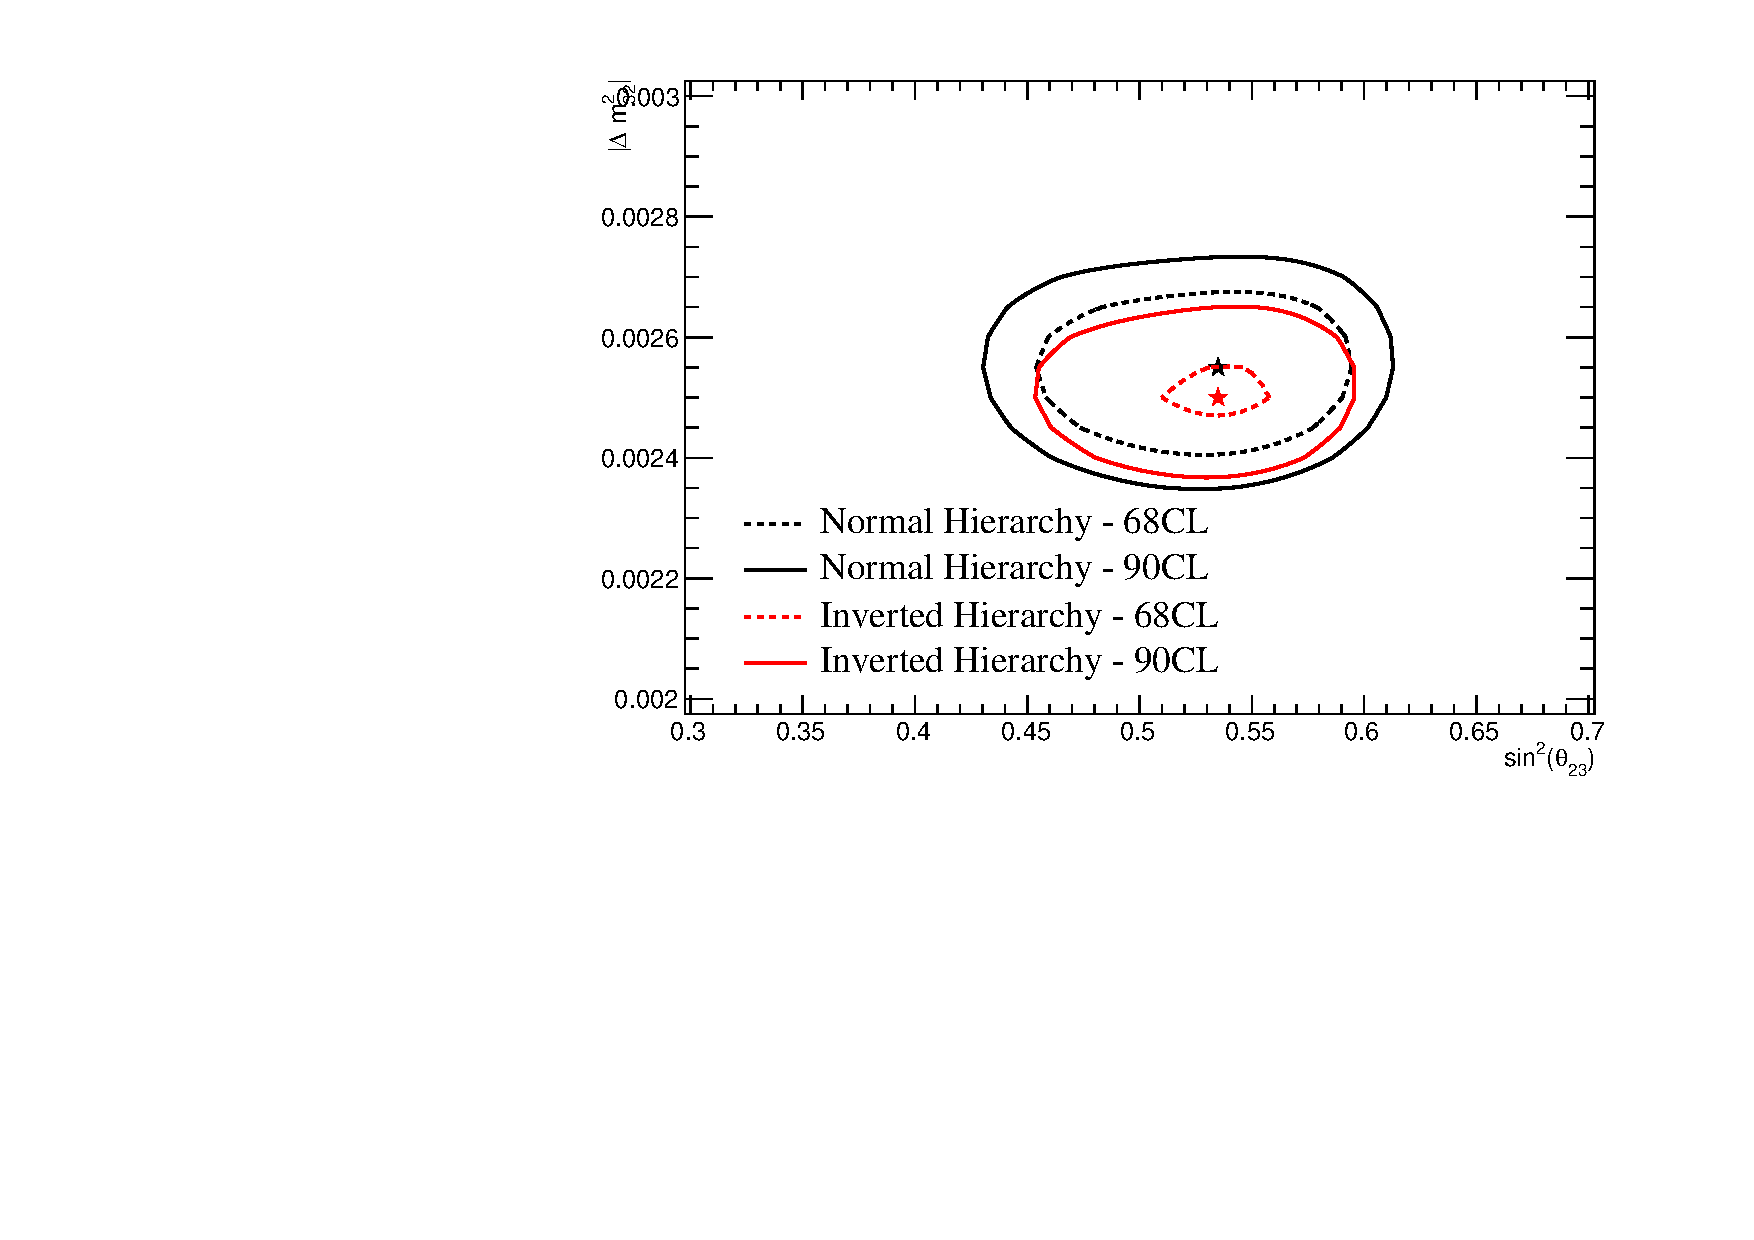
\includegraphics[width=0.9\textwidth]{joint_plots/data_contours/sinsqth23Vsdmsq_react_data_constdchisq_glob.pdf}
\caption{$\sin^2 \theta_{23}$ Vs $\Delta m^2_{32}$ ($\Delta m^2_{13}$)
with reactor constraint}
\end{subfigure}
%
\includegraphics[width=0.9\textwidth]{./images/missing_plot-eps-converted-to.pdf}
%
\includegraphics[width=0.9\textwidth]{./images/missing_plot-eps-converted-to.pdf}
%
\includegraphics[width=0.9\textwidth]{./images/missing_plot-eps-converted-to.pdf}
%
\includegraphics[width=0.9\textwidth]{./images/missing_plot-eps-converted-to.pdf}
%
\includegraphics[width=0.9\textwidth]{./images/missing_plot-eps-converted-to.pdf}
\caption{
%{\large{MEASURED 2D CONTOURS}}
Measured confidence intervals 
with the full run 1-6 data set.
Both normal (black) and inverted (red) hierarchies are shown. 
Contours for normal (black) and inverted (red) hierarchy are computed 
with respect to the minimum of the best-fit hierarchy (star), which
corresponds to normal hierarchy.
Both 68\% (dashed line) and 90\% CL (solid line) are shown.
Confidence intervals are produced using the \emph{constant} $\Delta \chi^2$ method. % (see app.~\ref{app:method_cl}).
All the oscillation parameters which are not parameters of interest
are marginalised using the prior distributions shown in tab.~\ref{tab:osc_params_joint_priors}.
The measured contour of $\sin^2 \theta_{13}$ Vs $\delta_{CP}$ without reactor constraint
is compared with the measurement by reactor experiments, 
$\sin^2 \theta_{13} = 0.0219 \pm 0.0012 $
\cite{pdg_2014},
shown by the yellow bar.
}
\label{fig:joint_sensi_t2krun14bf_2d_glob}
\end{figure*}


\begin{figure*}[htb]
\center
\begin{subfigure}[b]{0.49\textwidth}
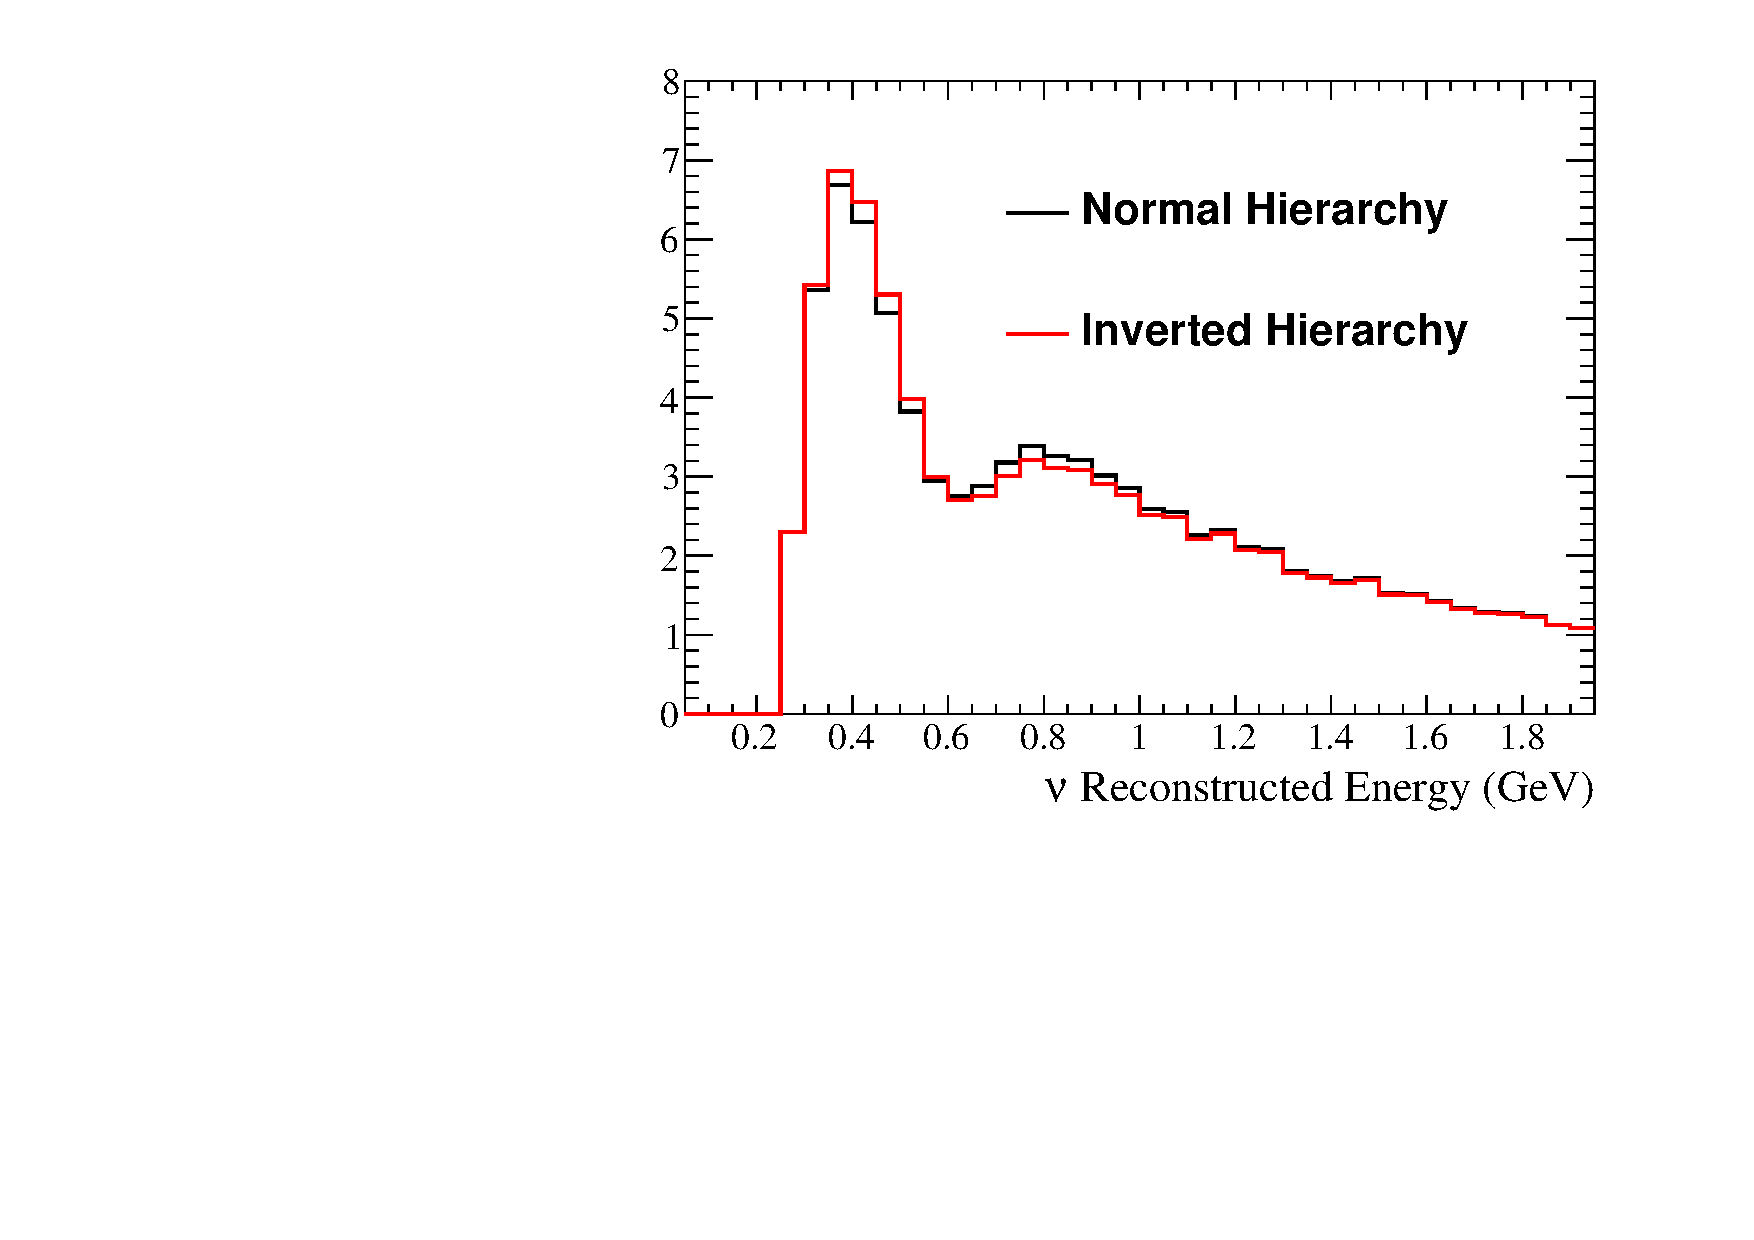
\includegraphics[width=0.9\textwidth]{joint_plots/spectrum_predictions/ereco_nh_Vs_ih_Asimov_A_1Rmu.pdf}
\caption{Muon-like, neutrino mode}
\end{subfigure}
\begin{subfigure}[b]{0.49\textwidth}
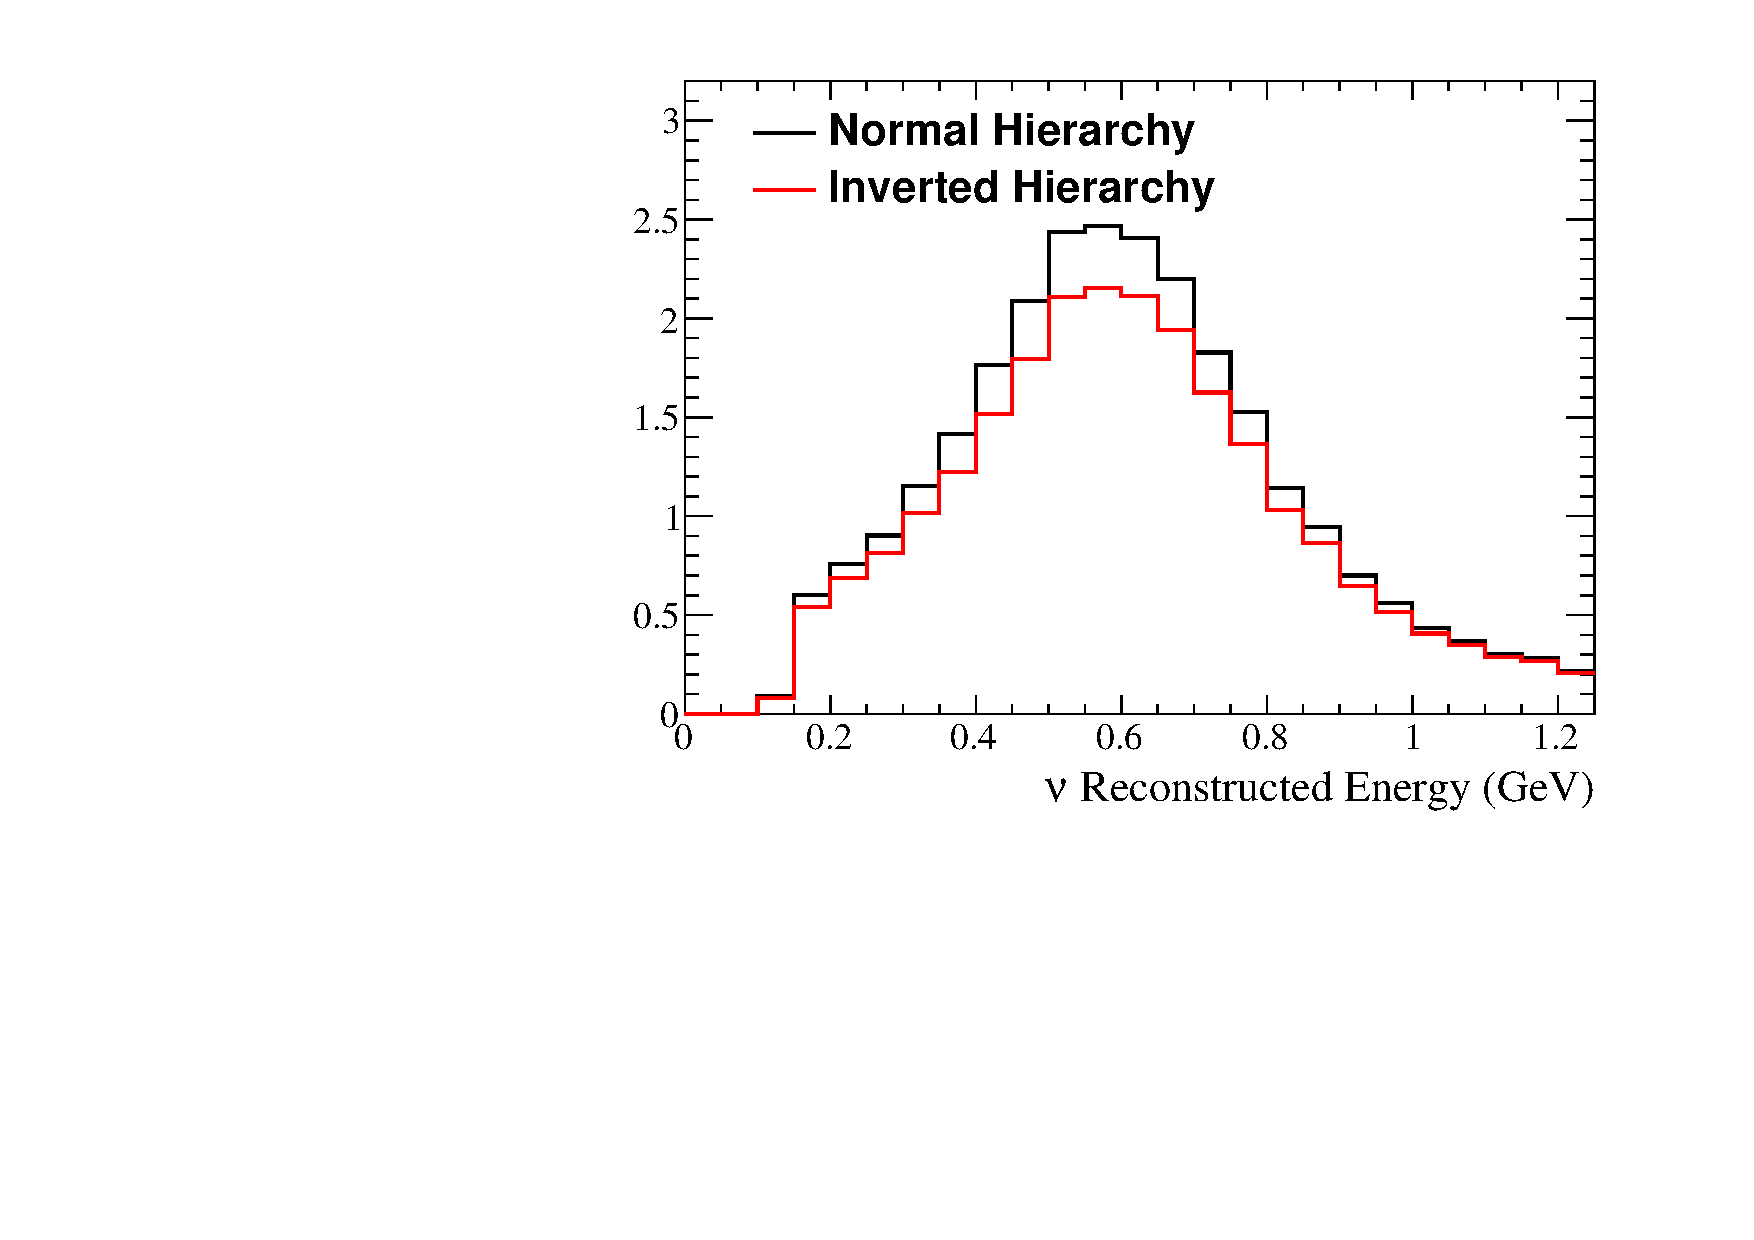
\includegraphics[width=0.9\textwidth]{joint_plots/spectrum_predictions/ereco_nh_Vs_ih_Asimov_A_1Re.pdf}
\caption{Electron-like, neutrino mode}
\end{subfigure}
\begin{subfigure}[b]{0.49\textwidth}
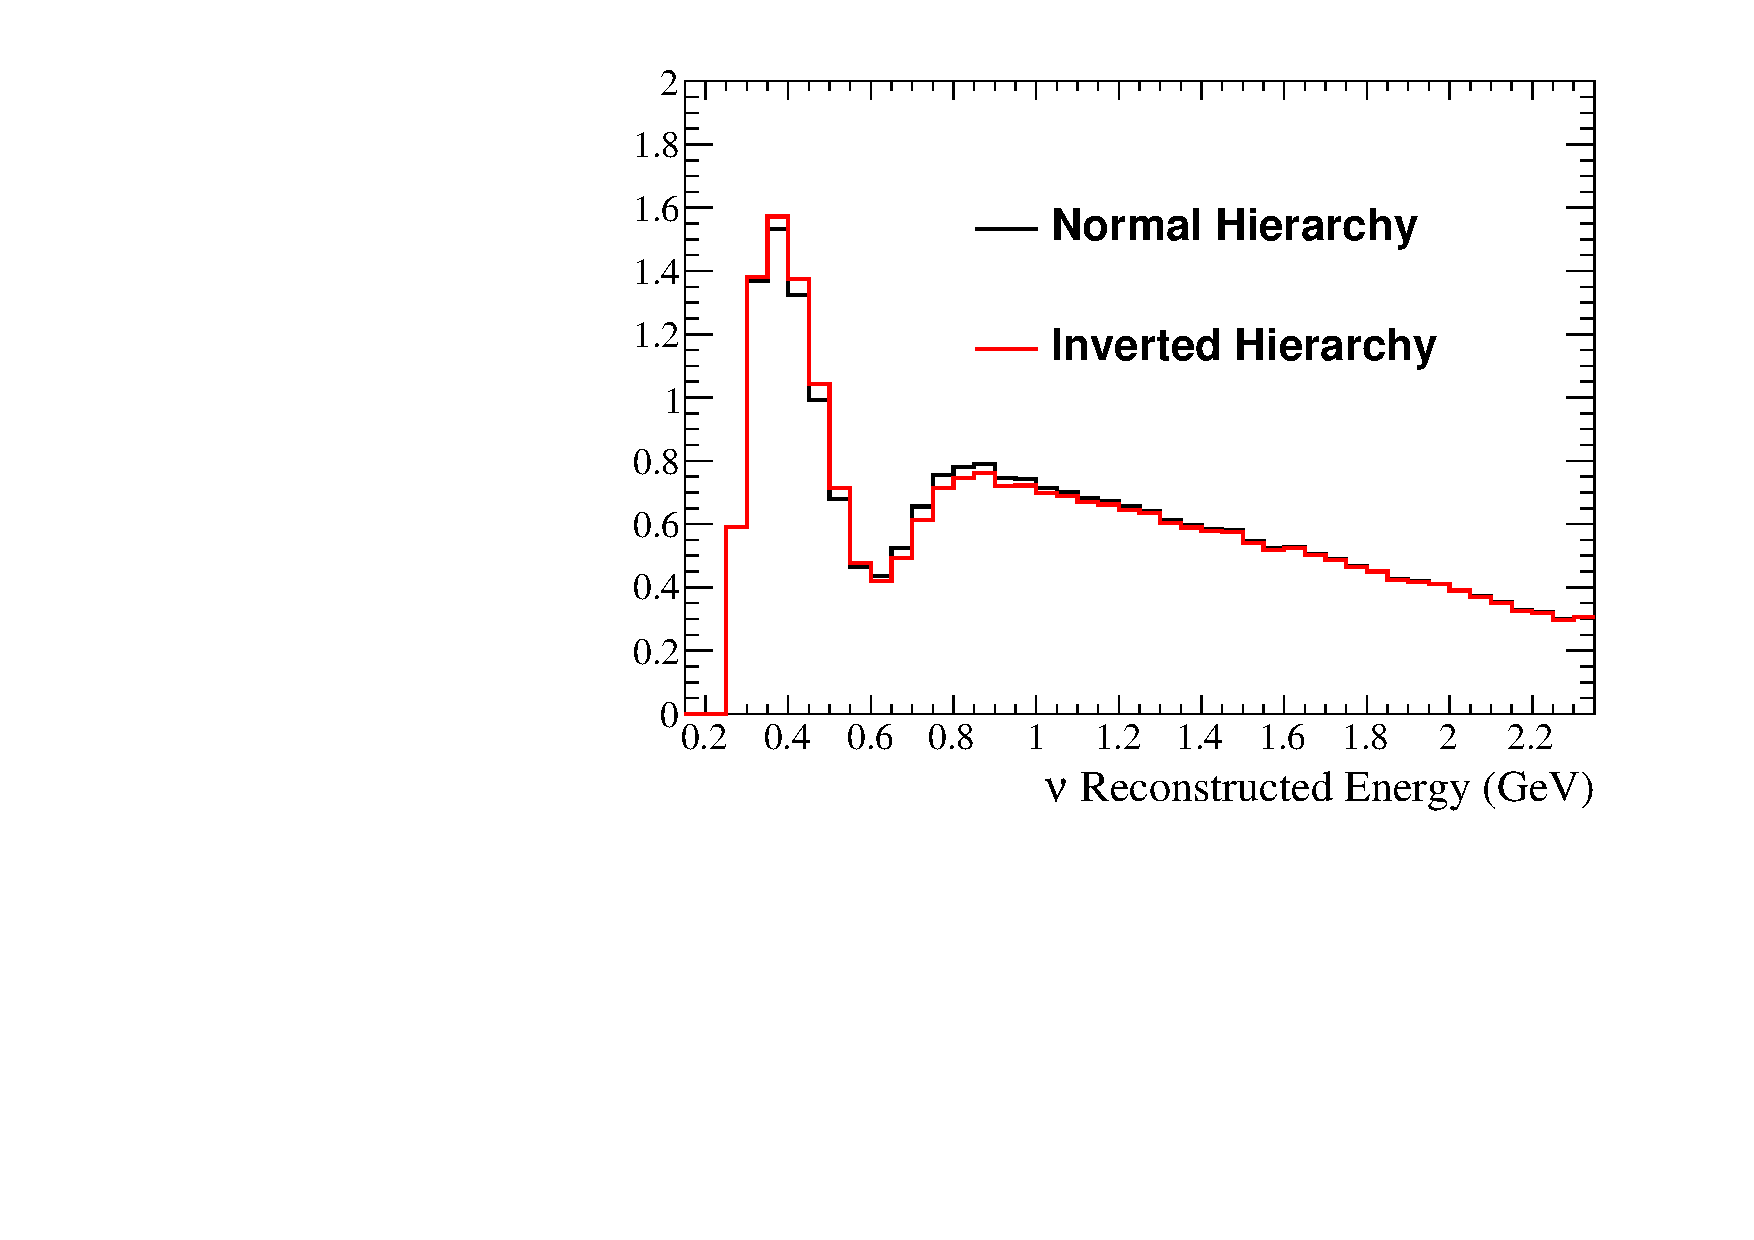
\includegraphics[width=0.9\textwidth]{joint_plots/spectrum_predictions/ereco_nh_Vs_ih_Asimov_A_RHC1Rmu.pdf}
\caption{Muon-like, antineutrino mode}
\end{subfigure}
\begin{subfigure}[b]{0.49\textwidth}
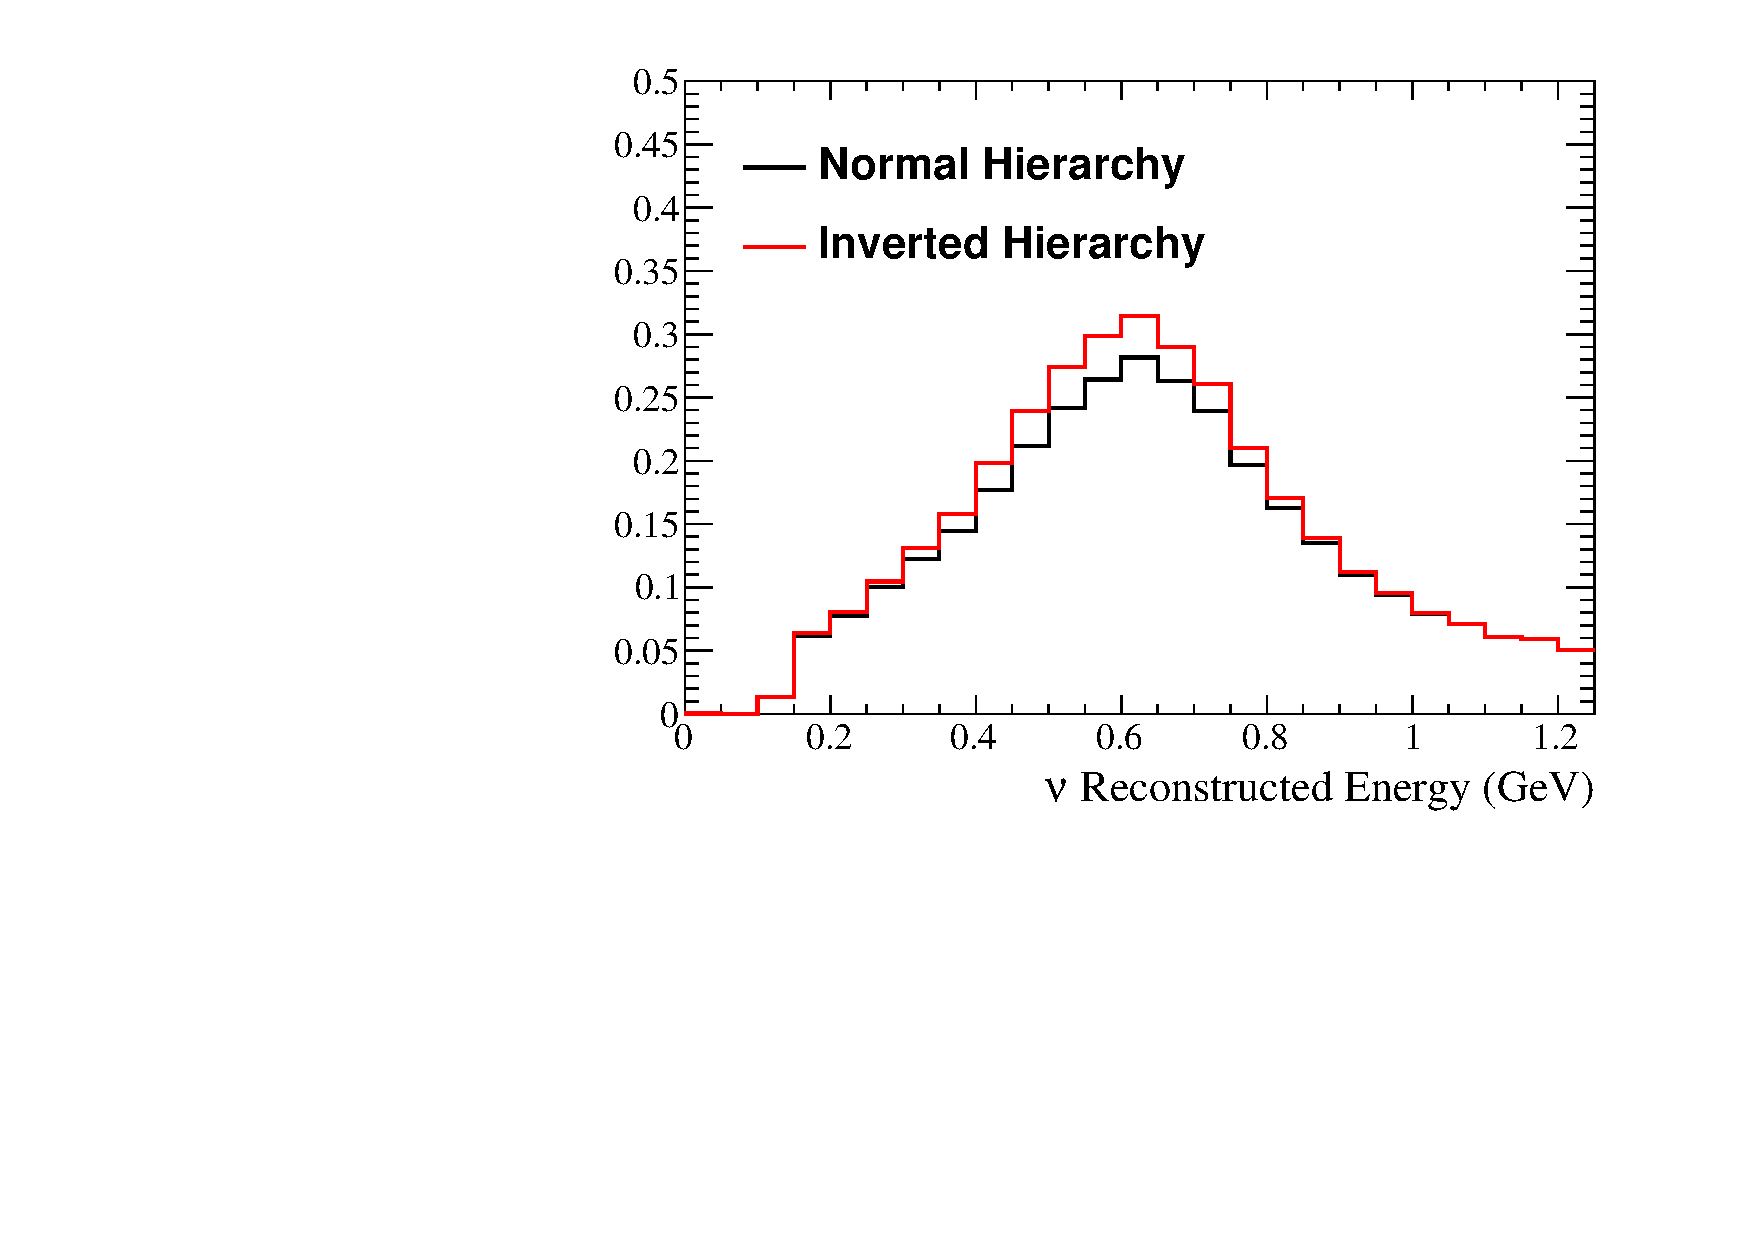
\includegraphics[width=0.9\textwidth]{joint_plots/spectrum_predictions/ereco_nh_Vs_ih_Asimov_A_RHC1Re.pdf}
\caption{Electron-like, antineutrino mode}
\end{subfigure}
%\includegraphics[width=0.9\textwidth]{joint_plots/data/1rmu_ereco_tot_osc_notosc_bf.pdf}
%\includegraphics[width=0.9\textwidth]{joint_plots/data/rhc1rmu_ereco_tot_osc_notosc_bf.pdf}
%\includegraphics[width=0.9\textwidth]{joint_plots/data/1re_ereco_tot_osc_notosc_bf.pdf}
%\includegraphics[width=0.9\textwidth]{joint_plots/data/rhc1re_ereco_tot_osc_notosc_bf.pdf}
\caption {
%    \huge{TO UPDATE} % caption is already ok
%{\large{MEASURED BEST-FIT ERECO SPECTRA COMPARED TO DATA AND 
%PREDICTED UNOSCILLATED SPECTRA}}
The expected spectra as a function of the neutrino reconstructed energy
are shown for each selected sample
of the run 1-6 data set
for both normal (black) and inverted (red) hierarchies.
They correspond to the Asimov data set A
in~\cref{tab:osc_params_joint_asimov}
and are generated with the systematic parameters measured with the ND280 data 
shown in tab.~\ref{tab:banff_uncertainties_flux_fhc},
~\ref{tab:banff_uncertainties_flux_rhc},
~\ref{tab:banff_uncertainties_xsec}
and~\ref{tab:banff_uncertainties_skdetfsi}.
}
\label{fig:mass_hierarchy_MC_shift}
\end{figure*}



%%...........................................................
%%
%% Goodness of fit
%%
%%...........................................................
%
%\subsection{Goodness of fit}
%\label{sec:results_gof}
%
%The goodness of fit study is performed using the best fit spectra described in sec.~\ref{sec:method_gof}.
%All the oscillation as well as the systematic parameters are marginalised except $\delta_{CP}$,
%which is fixed to its best-fit value, since in the analysis it is minimised.
%The result corresponds to T2K only data.

%The p-values from these tests show that the fits are plausible for both mass hierarchies.

%\vspace{3mm}
%{\huge{
%TODO: ADD COMMENTS ABOUT GOF AND P-VALUE RESULT
%}}
%\vspace{3mm}
%
%\begin{figure*}[htb]
%\center
%
\includegraphics[width=0.9\textwidth]{./images/missing_plot-eps-converted-to.pdf}
%\caption{
%    \huge{TO UPDATE} % caption is already ok
%{\large{MEASURED GOODNESS OF FIT}}
%%Distribution of $\chi^2$ , the goodness-of-fit (gof) $\chi^2$, from 1k toy MC experiments whose true input value
%%is the best-fit $\delta_{CP}$ value from the fit of the real Run 1-6 data set (see Tab.~\ref{tab:joint_bestfit}).
%%Systematic variations and statistical fluctuations are applied to the toy datasets, 
%%and all \NSyst{} systematic parameters are included in the fits. 
%%The toy experiments are generated
%%for an exposure 
%%of $6.914 \times 10^{20}$ POT in neutrino mode
%%and
%%of $4.011 \times 10^{20}$ POT in antineutrino mode.
%%and the normal mass hierarchy, favored by the fit of the data, is assumed. 
%%The $\chi^2$ value from the fit of the real data assuming the normal mass hierarchy 
%%(with all \NSyst{} systematic parameters included in the fit) is shown as a red line.
%}
%\label{fig:joint_gof}
%\end{figure*}



%...........................................................
%
% Discussion about the results
%
%...........................................................

\subsection {Discussion of the results}
\label{sec:results_discussion}

The value of $\delta_{CP}$ favored by the joint fit analysis when the reactor constraint is applied 
is -1.854 and corresponds to normal hierarchy.
$\delta_{CP} = 0$ is excluded at 90\% CL and a large fraction of the range between $\delta_{CP} = 0$ and $+\pi$
is excluded with a significance of $2 \sigma$ (with the constant $\Delta \chi^2$ method).
The inverted hierarchy is disfavored at more than $\sim 1 \sigma$ level and it is partially 
excluded at $3\sigma$ for values of $\delta_{CP}$ around $+\pi/2$.
It has been shown this exclusion, stronger than what is expected from the fit of the Asimov data sets for $\delta_{CP}=-1.601$,
is due to the small excess of events in the neutrino mode $e$-like sample. 
Indeed the impact of antineutrino mode samples on the result is quite small.
If the reactor constraint is not applied, the best-fit value of $\delta_{CP}$ is still quite close to $-\pi/2$.
However the exclusion is much weaker than when the reactor constraint is applied.
The contour of $\sin^2 \theta_{13}$ Vs $\delta_{CP}$ shows
an agreement at the level of $1 \sigma$ with the measurement of the reactors if $\delta_{CP} \sim -\pi/2$.

The result shows a stronger exclusion of $\delta_{CP}$ compared to the 2014 joint fit analysis \cite{OurRun1234JointOscillationAnalysis}.
This is mainly due to the new reactor constraint which has lower $\sin^2 \theta_{13}$ (0.0217 instead of 0.0250)
and a smaller uncertainty:
$0.085 \pm 0.005$ instead of
$0.095 \pm 0.01$.

%\vspace{3mm}
%{\huge{
%TODO: ADD COMMENTS ABOUT RESULTS
%}}
%\vspace{3mm}


\clearpage



%%...........................................................
%%
%% Summary of the results of all the analyses
%%
%%...........................................................
%
%\subsection {Comparison with results from other analyses}
%\label{sec:results_other_analyses}
%
%\begin{figure*}[htb]
%\center
%
\includegraphics[width=0.9\textwidth]{./images/missing_plot-eps-converted-to.pdf}
%
\includegraphics[width=0.9\textwidth]{./images/missing_plot-eps-converted-to.pdf}
%
\includegraphics[width=0.9\textwidth]{./images/missing_plot-eps-converted-to.pdf}
%\caption{
%{\large{COMPARISON OF OUR WITH OTHER ANALYSIS MEASURED CONTOURS}}
%}
%\label{fig:joint_contour_comparison}
%\end{figure*}
%
%\vspace{3mm}
%{\huge{
%TODO: ADD COMMENTS ABOUT COMPARISONS
%}}
%\vspace{3mm}
%






\clearpage







\clearpage

% --------------------------------------------------------------------------------------------

\section {$\bar{\nu}_e$ appearance analysis}
\label{sec:nuebarapp}

The significance to $\bar{\nu}_e$ appearance was given as a p-value.
The marginalisation method is used and all the Super-K samples are analyzed simultaneously.
The oscillation parameters priors used for the marginalisation are shown in \cref{tab:osc_params_joint_priors}.
Two different test statistics were used: rate-only and rate+shape

\subsection{Rate-only analysis method}
\label{sec:nuebarapp_rateonly}

The total number of observed events ($N_{obs}$), without using any information from the 
reconstructed energy shape, was used to quote the rate-only p-value. 
In order to simultaneously analyze 
all the Super-K samples a different procedure with respect to the one used in 2015 analysis
\cite{OurRun56AntiNueBarAppearanceAnalysis3Flavour}, 
where toys were performed by using the posterior distributions of the Run 1-4 Bayesian analysis,
has been adopted. 
For a single fit the following procedure was used:

\begin{itemize}
\item $N_{marg}$ toy experiments were performed taking into account only systematic uncertainties, but not the statistical fluctuations
\item For each toy the likelihood $\lambda_{marg}$ was calculated using eq.~\ref{eq:likemarg} and including only the samples which are not 
	affected by $\bar{\nu}_e$ appearance: neutrino mode muon-like, neutrino mode electron-like and antineutrino mode muon-like (called ``other samples")
\item Using the likelihood as a probability distribution function, 
	$\lambda_{marg}$ was then applied as a weight to the total number of observed events (of the toy) in the antineutrino mode electron-like sample
\item The procedure is repeated for all the $N_{marg}$ toy experiments. 
\end{itemize}

$N_{marg}$ is the number of marginalization toy experiments, which are needed to marginalise the systematic parameters and 
must be distinguished from the toy experiments that are used as fake-data sets in order to perform the p-value calculation.
Indeed the latter toys are performed by applying both systematic and statistical uncertainties.

It is worth to note that reweighting the number of events with the likelihood computed with the ``other samples", 
is mathematically the same as performing a likelihood ratio fit of the ``other samples", taking the posterior distribution of the systematic parameters 
and using it to extract the systematic parameters in a toy experiment.

The advantage of this method is that correlations between all the samples are taken correctly into account.
In the 2015 analysis the oscillation parameters were extracted from the Run 1-4 posterior distributions of the Bayesian analysis,
but the flux, cross section and detector systematic parameters priors were unaffected by the Run 1-4 data fit.
The difference between the two methods is negligible since the antineutrino mode $e$-like sample has a much lower statistic 
compared to the other samples, however this new method allows to take all the correlations into account correctly and 
to perform the analysis in one single step without making two different fits, one to obtain the oscillation parameters priors and the other to fit the antineutrino mode $e$-like data.




\subsection{Rate+shape analysis method}
\label{sec:nuebarapp_rateshape}

The rate+shape analysis method is similar to what is described in \ref{sec:cl}, with 
the difference that the test statistic is defined as:
 
\begin{align}
\Delta \chi^2 = \chi^2(\beta=0) - \chi^2(\beta=1)
\end{align}

where $\beta$ is the discrete parameter of interest that can take only 0 or 1 values.
This test statistic simply compare the oscillation with the non-oscillation hypothesis
but does not use the best-fit $\chi^2$ value.
More details are given in sec.\ref{sec:pvalue_nuebarapp}.
The method is analogue to what was used in \cite{OurRun56AntiNueBarAppearanceAnalysis3Flavour},
with the only difference that now all the Super-K samples are fitted simultaneously
and not only the antineutrino mode $e$-like one.

%--------------------------------------------------------------------------------------------------------------------                                                                                    

\subsection {P-value}
\label{sec:pvalue_nuebarapp}

% Describe the p-values used for the analysis

There are different test statistics which can be used to quote a p-value,
as described in 
~\cite{slides_davide_pvalue_asg} % ASG talk
.
As proposed by the OA group, for this $\bar{\nu}_e$ appearance search two different p-values are quoted.
In order to quote the significance given null $\bar{\nu}_e$ appearance, the parameter of interest is set to $\beta=0$
and $n=10k$ toys are performed.
The systematic parameters are randomized taking into account the correlations as described in \cref{sec:systematics:inputs}.
Then the $E_{reco}$ Vs $\theta$ distribution is fluctuated with Poisson. 
Then the following p-values are calculated:
\begin{itemize}

\item p-value with rate-only analysis: the number of events is used as test statistics, without using the shape information of the reconstructed energy 
	distribution. The distribution $f(N_{SK})$ of the total number of Super-K events in a toy ($N_{SK}$) is obtained from the performed toys. 
	Then the number of events is measured from the data set ($N_{SK}^{obs}$) and
	the 1-sided (right tail) p-value is computed in the following way: 	
	
	\begin{equation}
	\text{p-value (right tail)} = \int_{N_{SK}^{obs}}^{+\infty} f(N_{SK}) d N_{SK}  = 
		\frac{ \sum_{ itoy=1 }^{n} w(N_{SK} \geq N_{SK}^{obs} )^{itoy} }{ n }
	\end{equation}
	\label{eq:pvalue_rateonly}
	
	where $w(N_{SK} \geq N_{SK}^{obs})$ is 1 if $N_{SK} \geq N_{SK}^{obs}$ otherwise 0.
	The distribution $f(N_{tot}^{toy})$ is expected to be discrete since it follows the Poisson distribution.
			 
	In an analogous way the left tail 1-sided p-value is computed as following:
		
	\begin{equation}
	\text{p-value (left tail)} = \int^{N_{SK}^{obs}}_{-\infty} f(N_{SK}) d N_{SK}  = 
		\frac{ \sum_{ itoy=1 }^{n} w(N_{SK} \leq N_{SK}^{obs} )^{itoy} }{ n }
	\end{equation}
	\label{eq:pvalue_rateonly}
		 
\item p-value with rate+shape analysis: the shape information of the reconstructed energy distribution is used.
	In this case the test statistic is used to compare the case of $\beta=0$ with $\beta=1$:
	
	\begin{equation}
	\Delta \chi^2 = \chi^2(\beta=0) - \chi^2(\beta=1)
	\end{equation}
	\label{eq:deltachisq_rateshape}

	where $\chi^2(\beta=0)$ and $\chi^2(\beta=1)$ are computed using \cref{eq:loglikemarg}.
	It is worth to note that the parameter $\beta$ is not fitted but fixed either to 0 or 1.
	The 1-sided p-value (right tail) is calculated as:

	\begin{equation}
	\text{p-value (right tail)} = \int_{\Delta \chi^2_{obs}}^{+\infty} f(\Delta \chi^2) d \Delta \chi^2  = 
		\frac{ \sum_{ itoy=1 }^{n} w(\Delta \chi^2 \geq \Delta \chi^2_{obs} )^{itoy} }{ n }
	\end{equation}
	\label{eq:pvalue_rateonly}
	
	where $w(\Delta \chi^2  \geq \Delta \chi^2 _{obs})$ is 1 if $\Delta \chi^2  \geq \Delta \chi^2 _{obs}$ otherwise 0.

	The 1-sided p-value (left tail) is calculated as:

	\begin{equation}
	\text{p-value (left tail)} = \int^{\Delta \chi^2_{obs}}_{-\infty} f(\Delta \chi^2) d \Delta \chi^2  = 
		\frac{ \sum_{ itoy=1 }^{n} w(\Delta \chi^2 \leq \Delta \chi^2_{obs} )^{itoy} }{ n }
	\end{equation}
	\label{eq:pvalue_rateonly}
	
\end{itemize}

The p-value will be calculated on the left or right tail depending on the position of the observed test statistic
in the expected distribution. For example, if the observed test statistic is on the left tail of the expected distribution of the
test statistic, a 1-sided p-value is computed on the left tail. Otherwise a 1-sided p-value on the right tail is computed. 

%--------------------------------------------------------------------------------------------------------------------                                                                                    

\clearpage


\section {Sensitivity to $\bar{\nu}_e$ appearance}
\label{sec:sensitivity_nuebarapp}

As discussed within the OA group, 
since there are not fitted parameters in the analysis, the validation can 
be done by comparing the rate-only with rate+shape p-values and 
checking if the corresponding distributions are reasonable.
Of course the final validation is given if all the oscillation analyses agree.
This is done by performing a sensitivity study to $\bar{\nu}_e$ appearance
both with the Asimov dataset, which consists of the most probable dataset
that is the nominal expected $E_{reco}$ Vs $\theta$ distribution ~\cite{Asimov},
as well as for toy distributions, given a value of $\beta$.

The significance to $\bar{\nu}_e$ appearance is quoted 
%for 
%\TotalPotRHC1RePOT
%both \FakePotLow and 
%\FakePotHigh POT
using the procedure described in \cref{sec:pvalue_nuebarapp}.
In order to quote the significance to $\bar{\nu}_e$ appearance a 1-sided p-value (right tail) is computed.
In addition an mean p-value is also computed by performing \NumToysLarge toys.

%--------------------------------------------------------------------------------------------------------------------

\subsection {Asimov rate-only p-value}
\label{subsec:rateonly}

The expected Asimov rate-only p-value is given by the Asimov dataset A for $\beta=1$. 
The corresponding oscillation parameters are shown in \cref{tab:osc_params_joint_asimov},
The distribution of the number of superK events used as test statistic is shown in \cref{fig:pvalue_rateonly}. 
The expected number of events is
%3.718 for \FakePotLow POT 
%and 4.183 for  \FakePotHigh POT. 
%The quoted p-value is 
%and 0.113 for \FakePotLow POT.
%and 0.0538 for \FakePotHigh POT.
3.218 and the quoted p-value is XXX.
In \cref{tab:summary_sensi_rateonly} the rate-only p-value is shown
for different numbers of observed events.

\begin{figure}
\center
%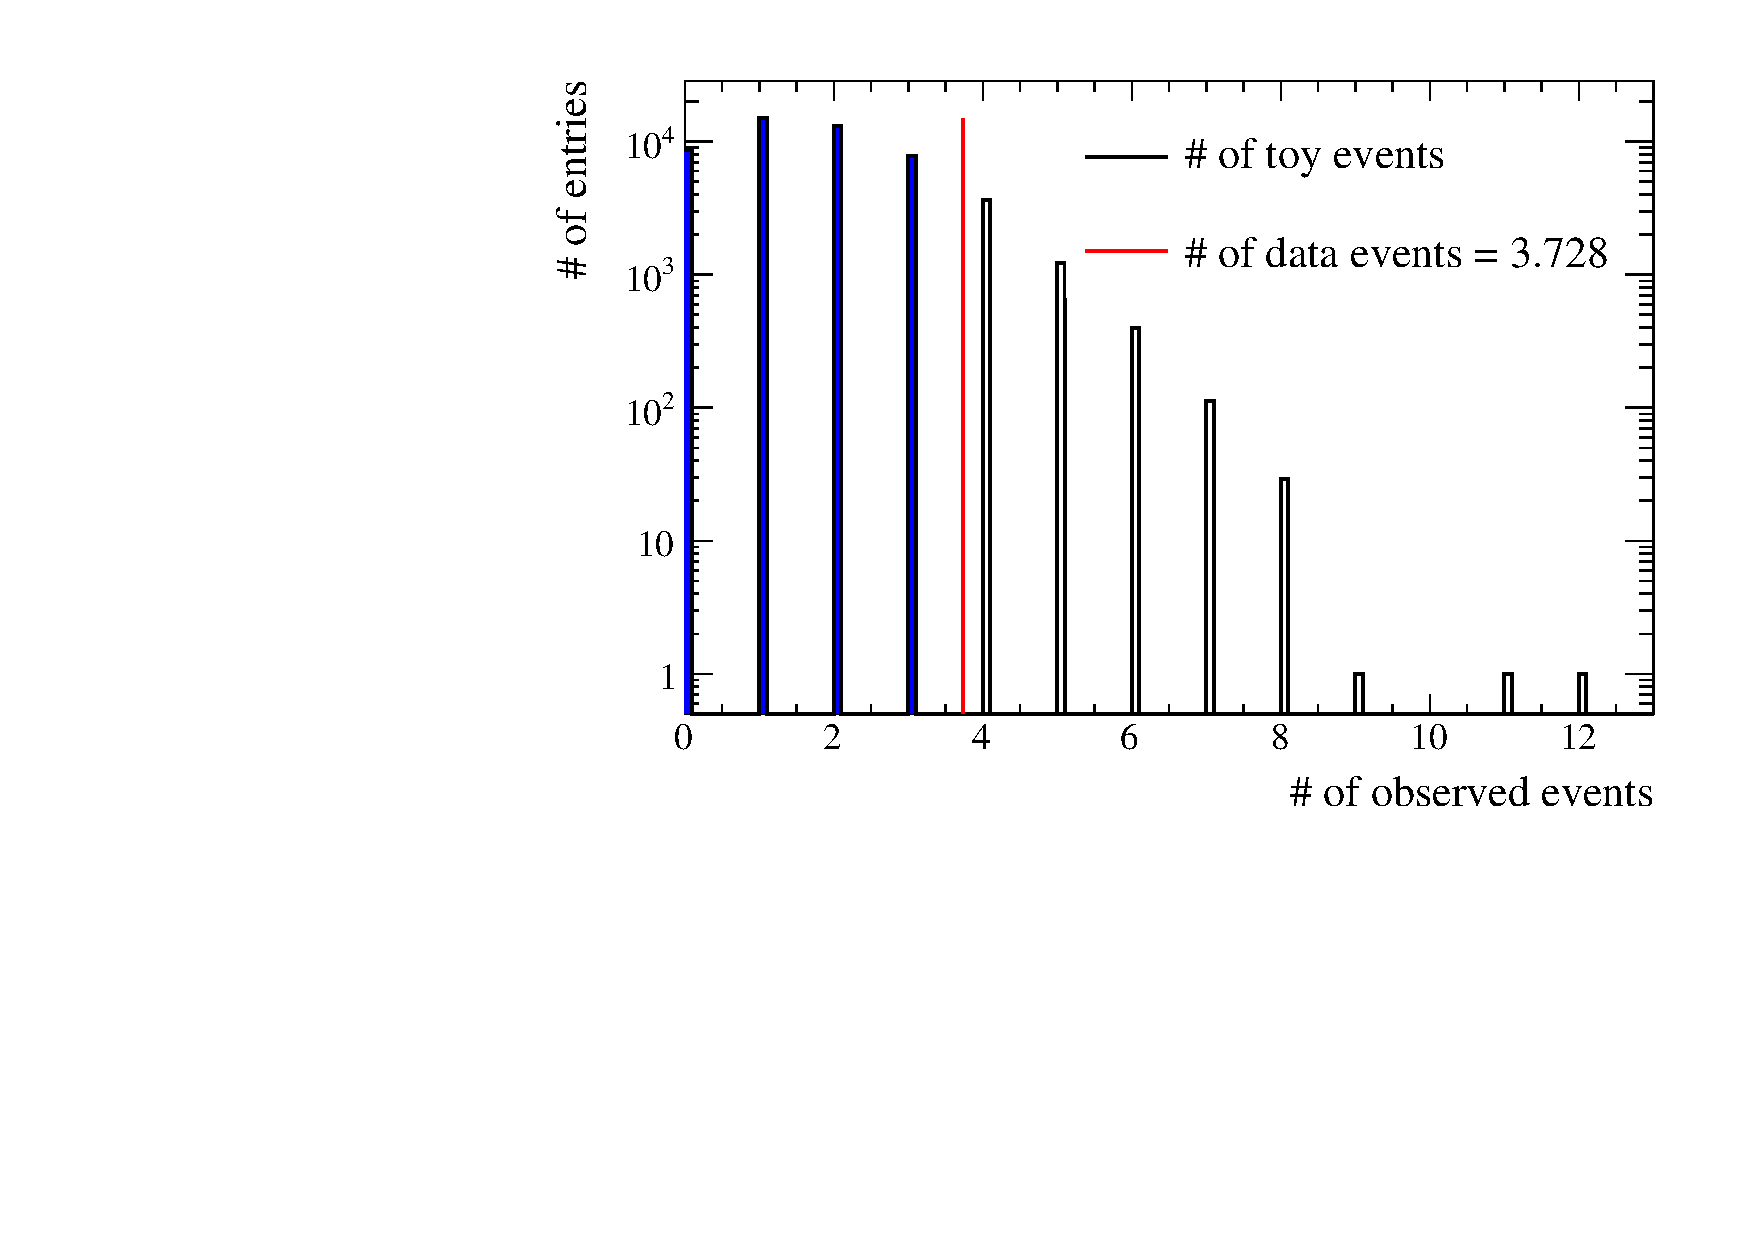
\includegraphics[width=0.9\textwidth]{./nuebar_plots/pvalue_median/pvalue_rate_4p0108E20POT_50ktoys.pdf}
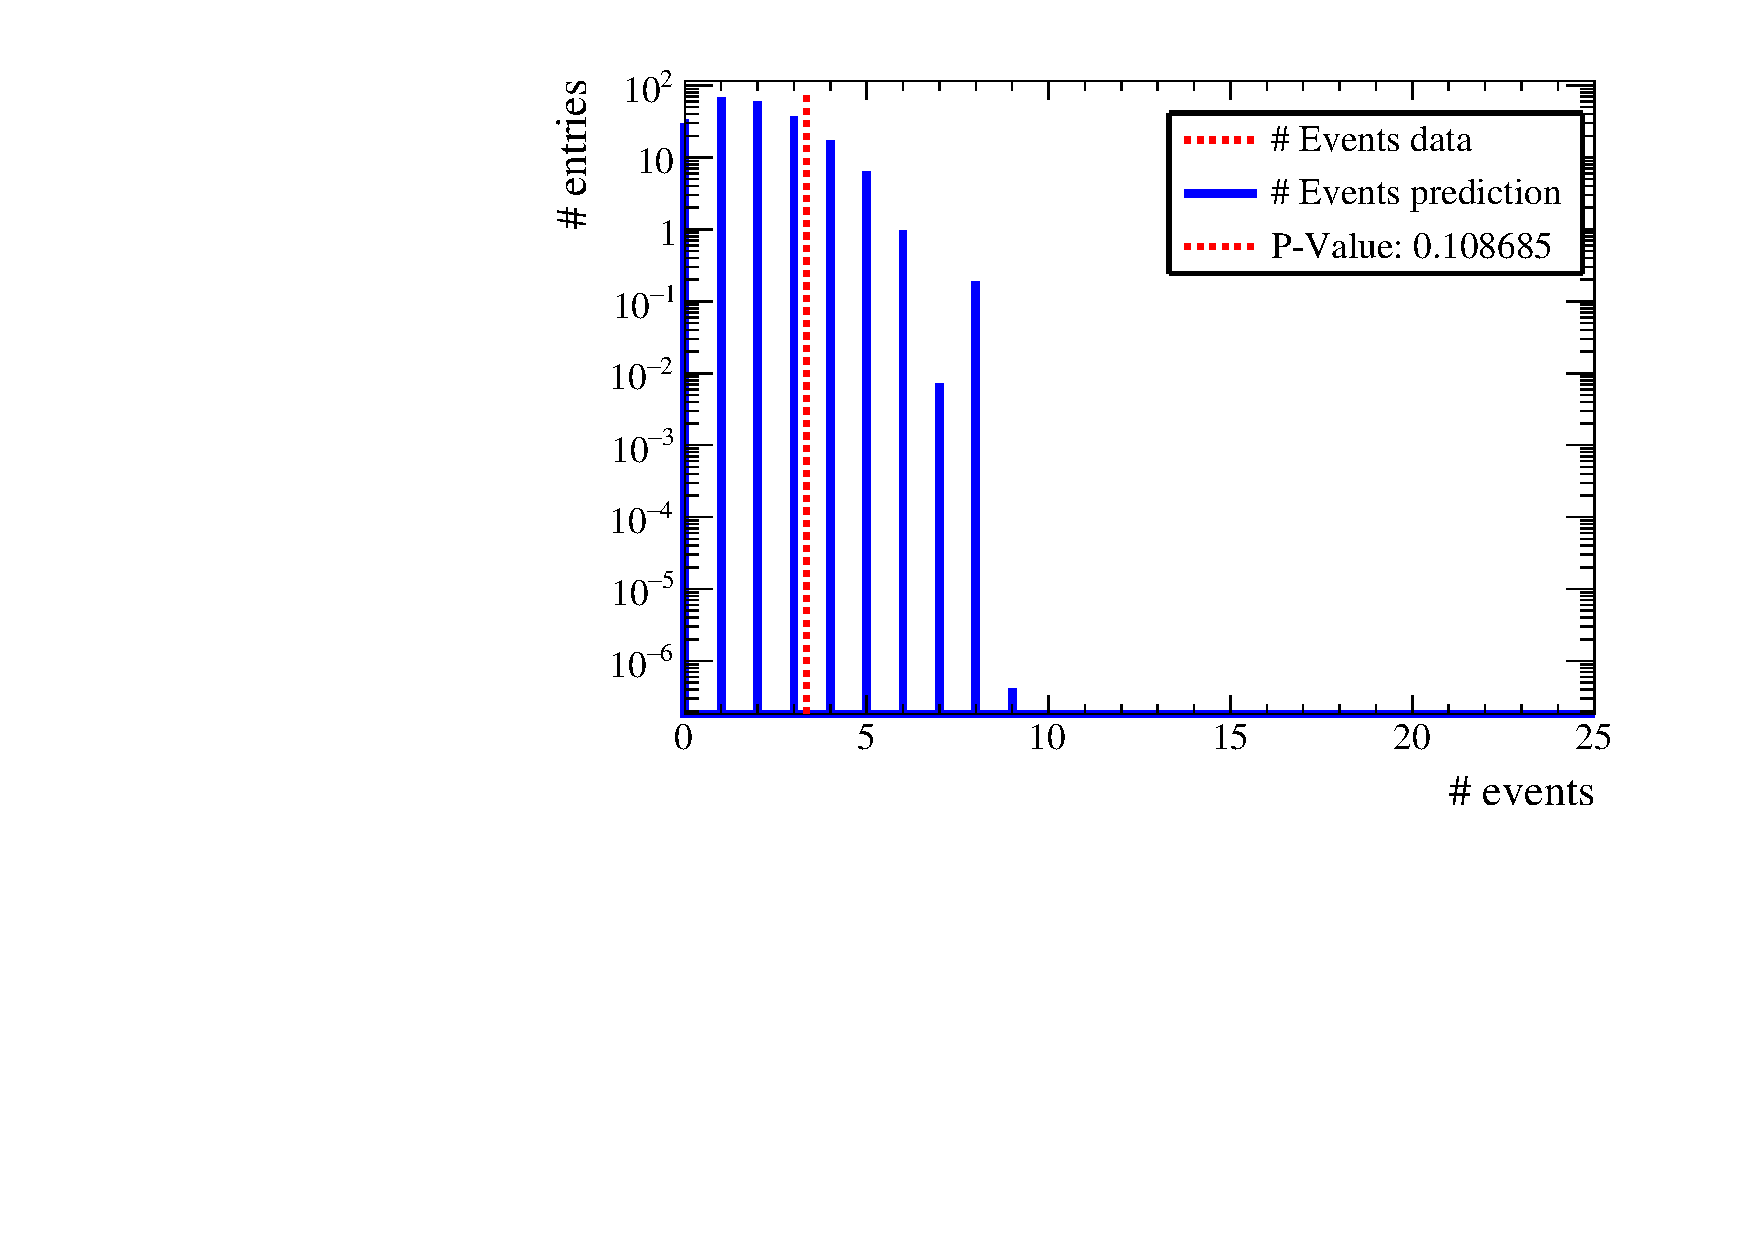
\includegraphics[width=0.6\textwidth]{./joint_plots/nuebar/rateonly/Asimov_beta1.pdf}
\caption {
%{\huge TO UPDATE} 
The distribution of the total number of events from each of the \NumToysLarge toy experiments. 
The red line corresponds to the total number of events given by the Asimov dataset. 
%The study is done with \TotalPotNuBar POT.
%\FakePotLow POT (left) and \FakePotHigh (right).
}
\label{fig:pvalue_rateonly}
\end{figure}

%--------------------------------------------------------------------------------------------------------------------




\subsection {Asimov rate+shape p-value}
\label{subsec:rateshape_median}


The expected distribution of $\Delta \chi^2$ for all the \NumToysLarge 
toy experiments
is shown in \cref{fig:pvalue_rateshape} for 
Run 1-6 statistic.
The $\Delta \chi^2$ from the Asimov dataset is 1.416.
The Asimov expected p-value is 0.0858 for the Run 1-6 statistic.

\begin{figure}
\center
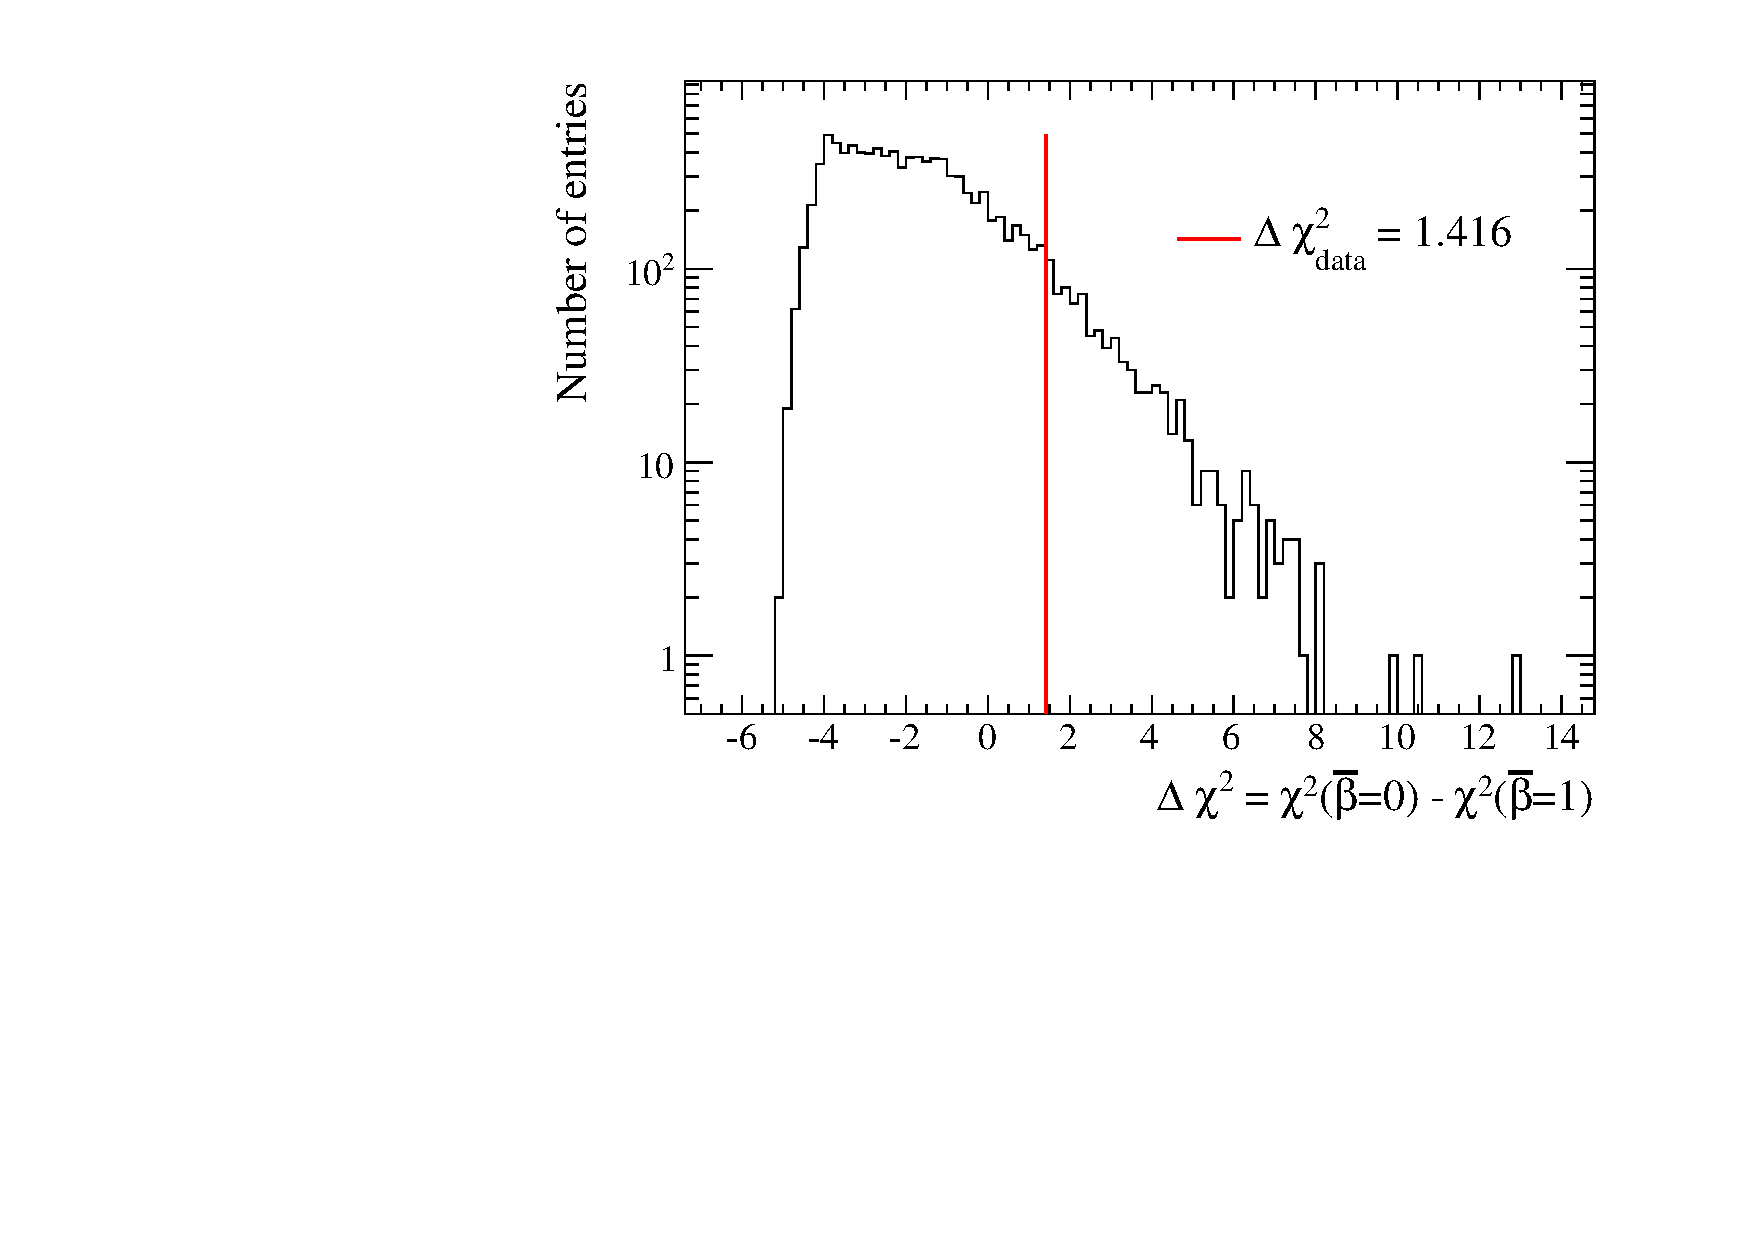
\includegraphics[width=0.48\linewidth]{./joint_plots/nuebar/rateshape/deltachisq_betabar_run16_10ktoys.pdf}
\caption {
Distribution of the $\Delta \chi^2$ for each of the \NumToysLarge 
toy experiments. 
The red line corresponds to $\Delta \chi^2$ obtained from the fit of the Asimov dataset A. 
The study is done with 
Run 1-6 statistic.
}
\label{fig:pvalue_rateshape}
\end{figure}

The p-value for the Asimov dataset as a function of $\beta$ or the total number of events is shown for 
Run 1-6 statistic
in \cref{fig:pvalue_Vs_beta_lowpot} and \cref{fig:pvalue_Vs_nevents_lowpot}. 

\begin{figure}
\center
%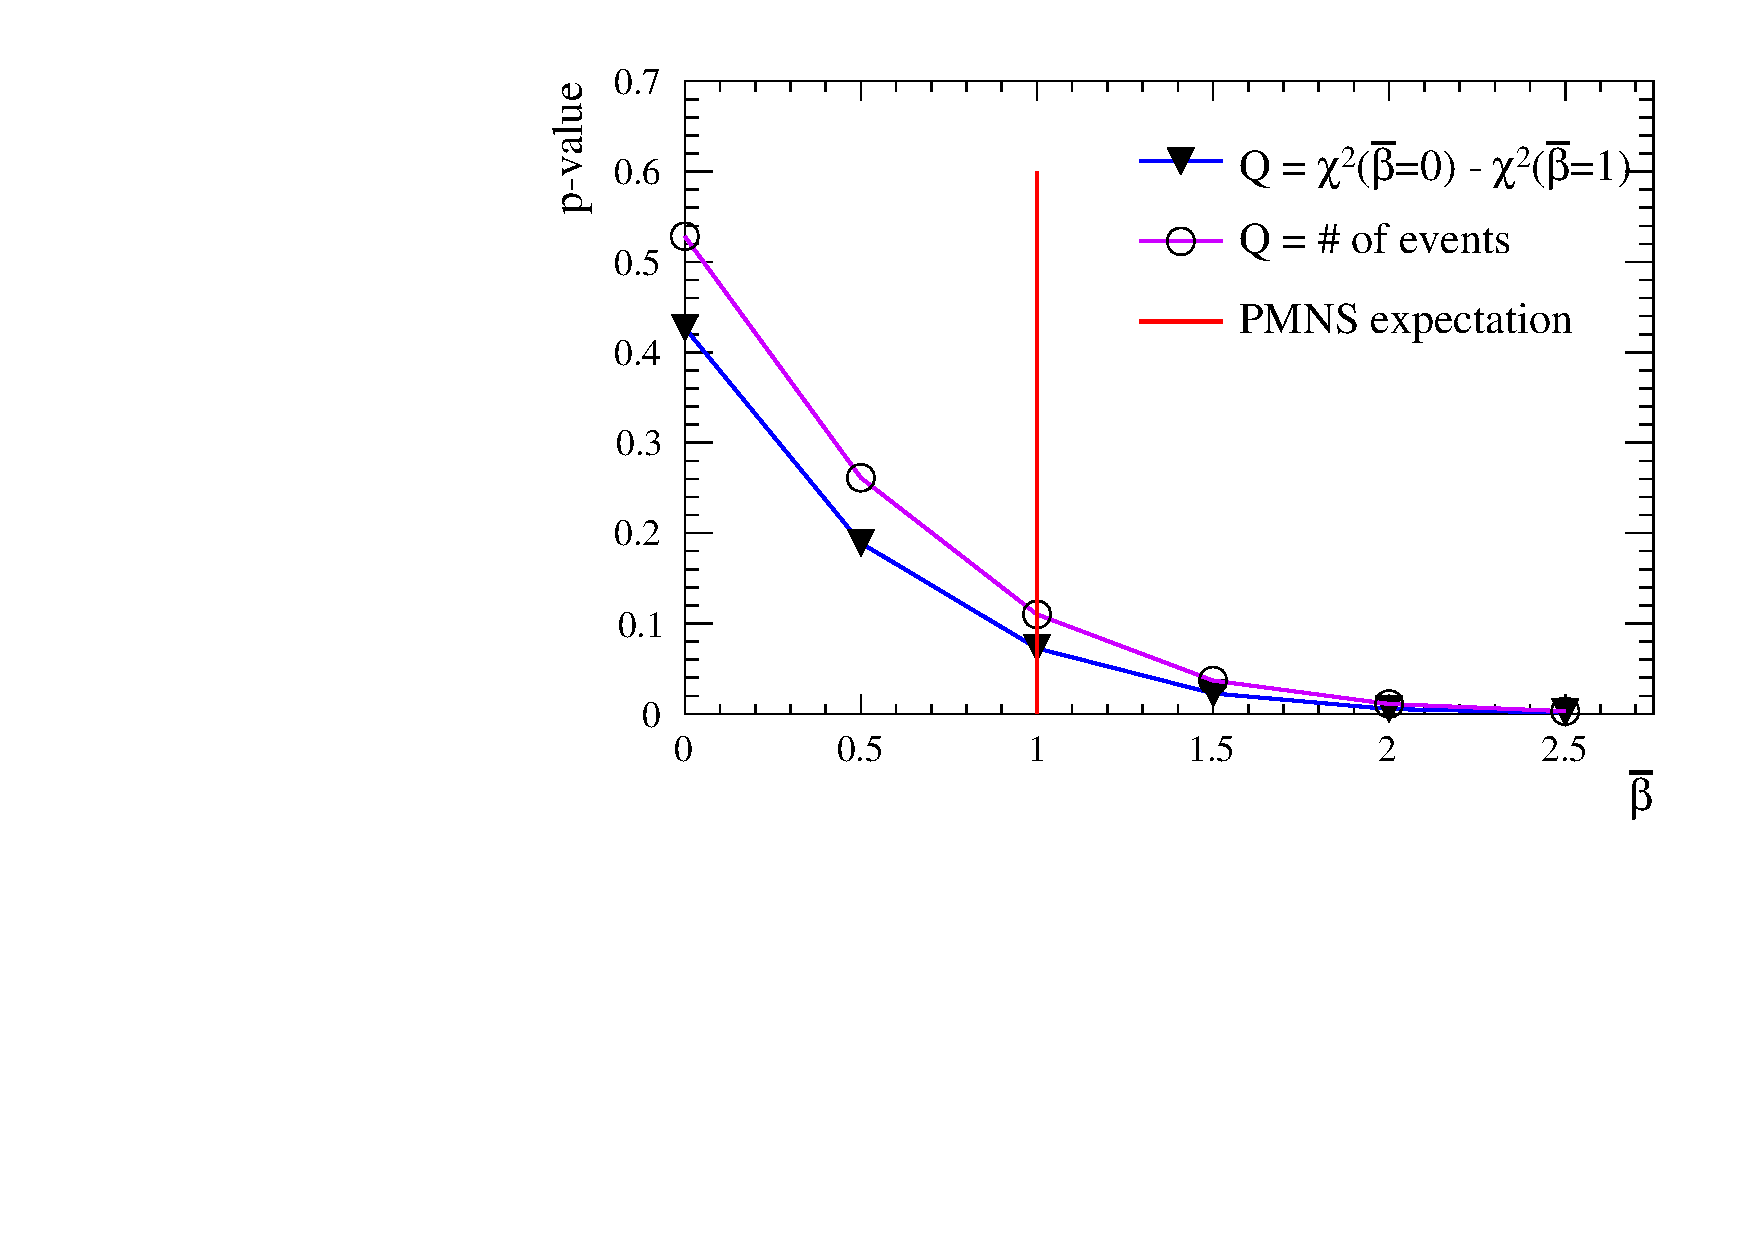
\includegraphics[width=0.48\linewidth]{./nuebar_plots/sensitivity/pvalue_Vs_beta_4p0108E20POT.pdf}
%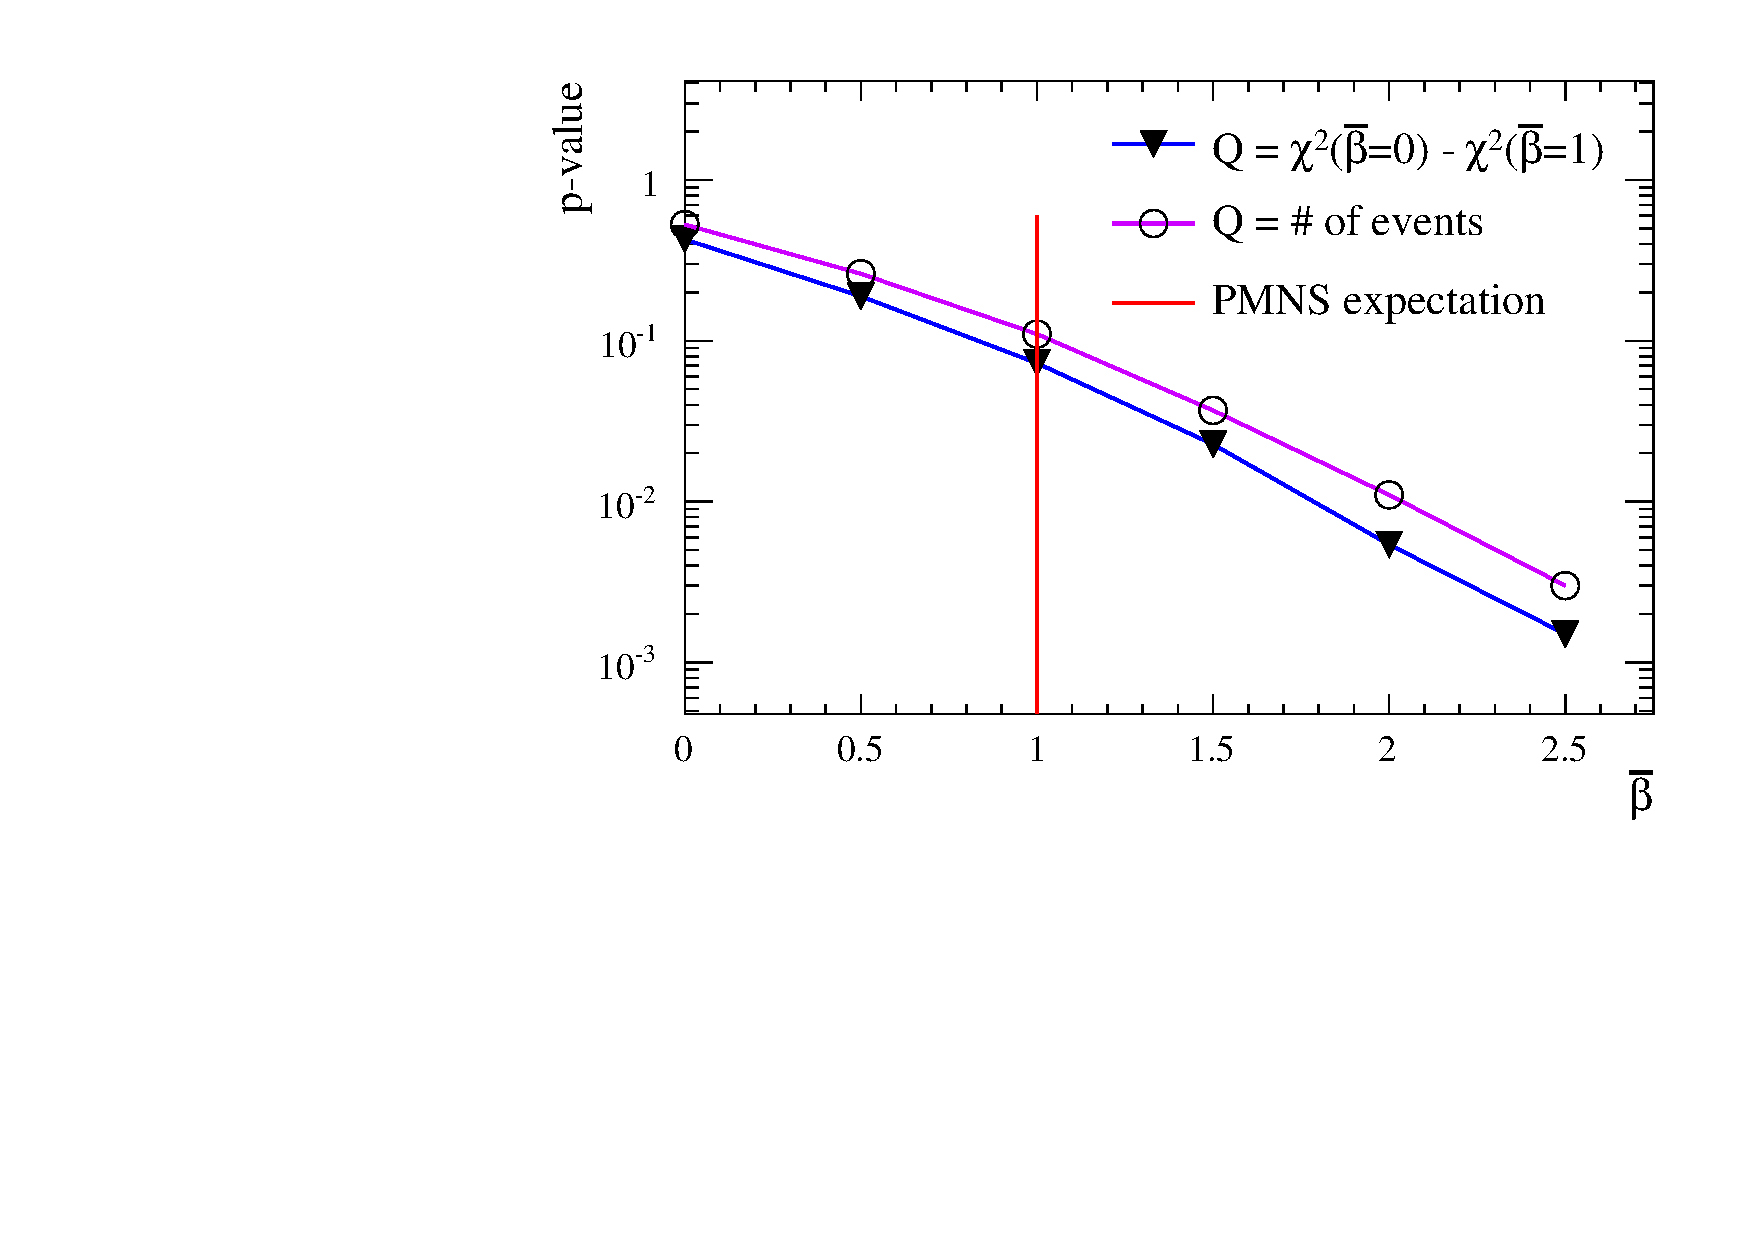
\includegraphics[width=0.48\linewidth]{./nuebar_plots/sensitivity/pvalue_Vs_beta_4p0108E20POT_log.pdf}
\begin{subfigure}[b]{0.49\textwidth}
\center
%
\includegraphics[width=0.9\textwidth]{./images/missing_plot-eps-converted-to.pdf}
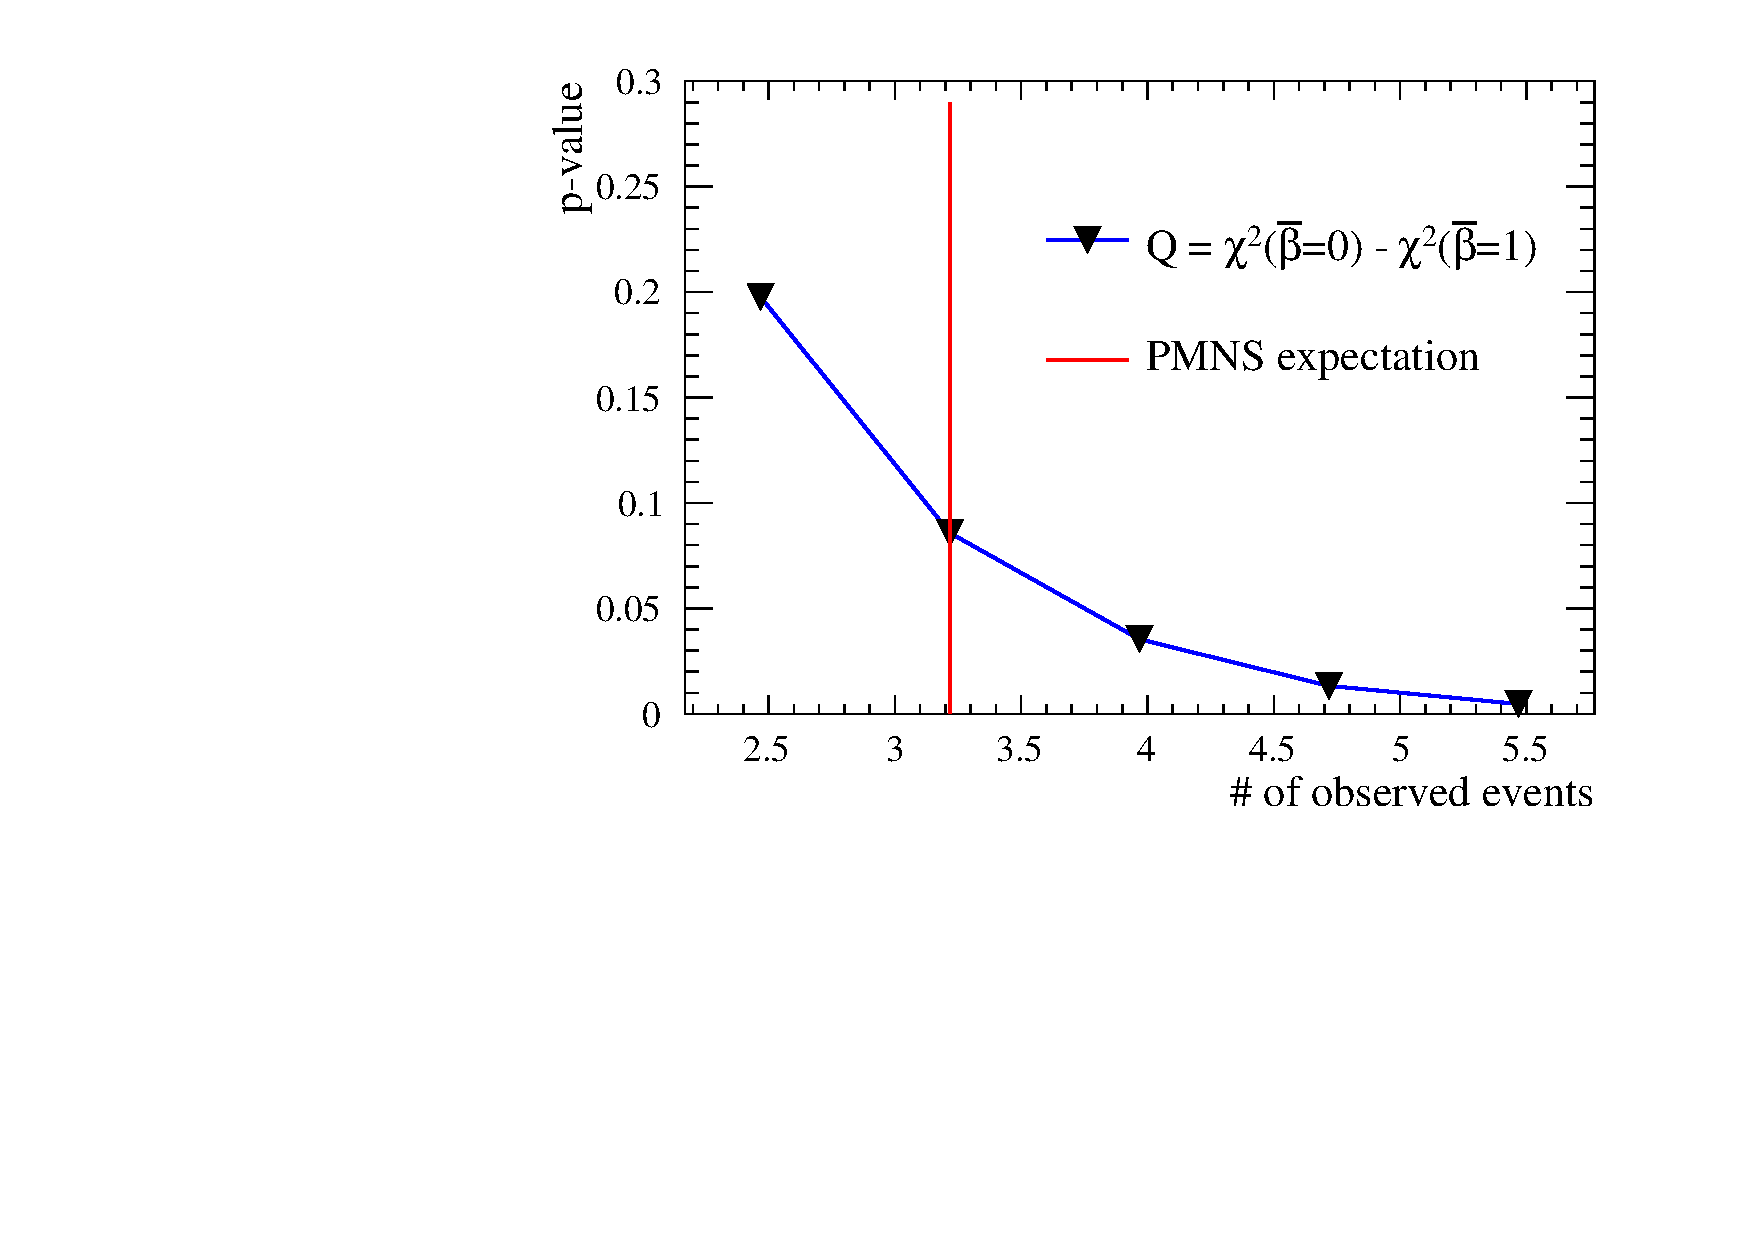
\includegraphics[width=0.9\linewidth]{./joint_plots/nuebar/rateshape/pvalue_Vs_nevt_ratepshape.pdf} 
\caption{Something}
\end{subfigure}
\begin{subfigure}[b]{0.49\textwidth}
\center
%
\includegraphics[width=0.9\textwidth]{./images/missing_plot-eps-converted-to.pdf}
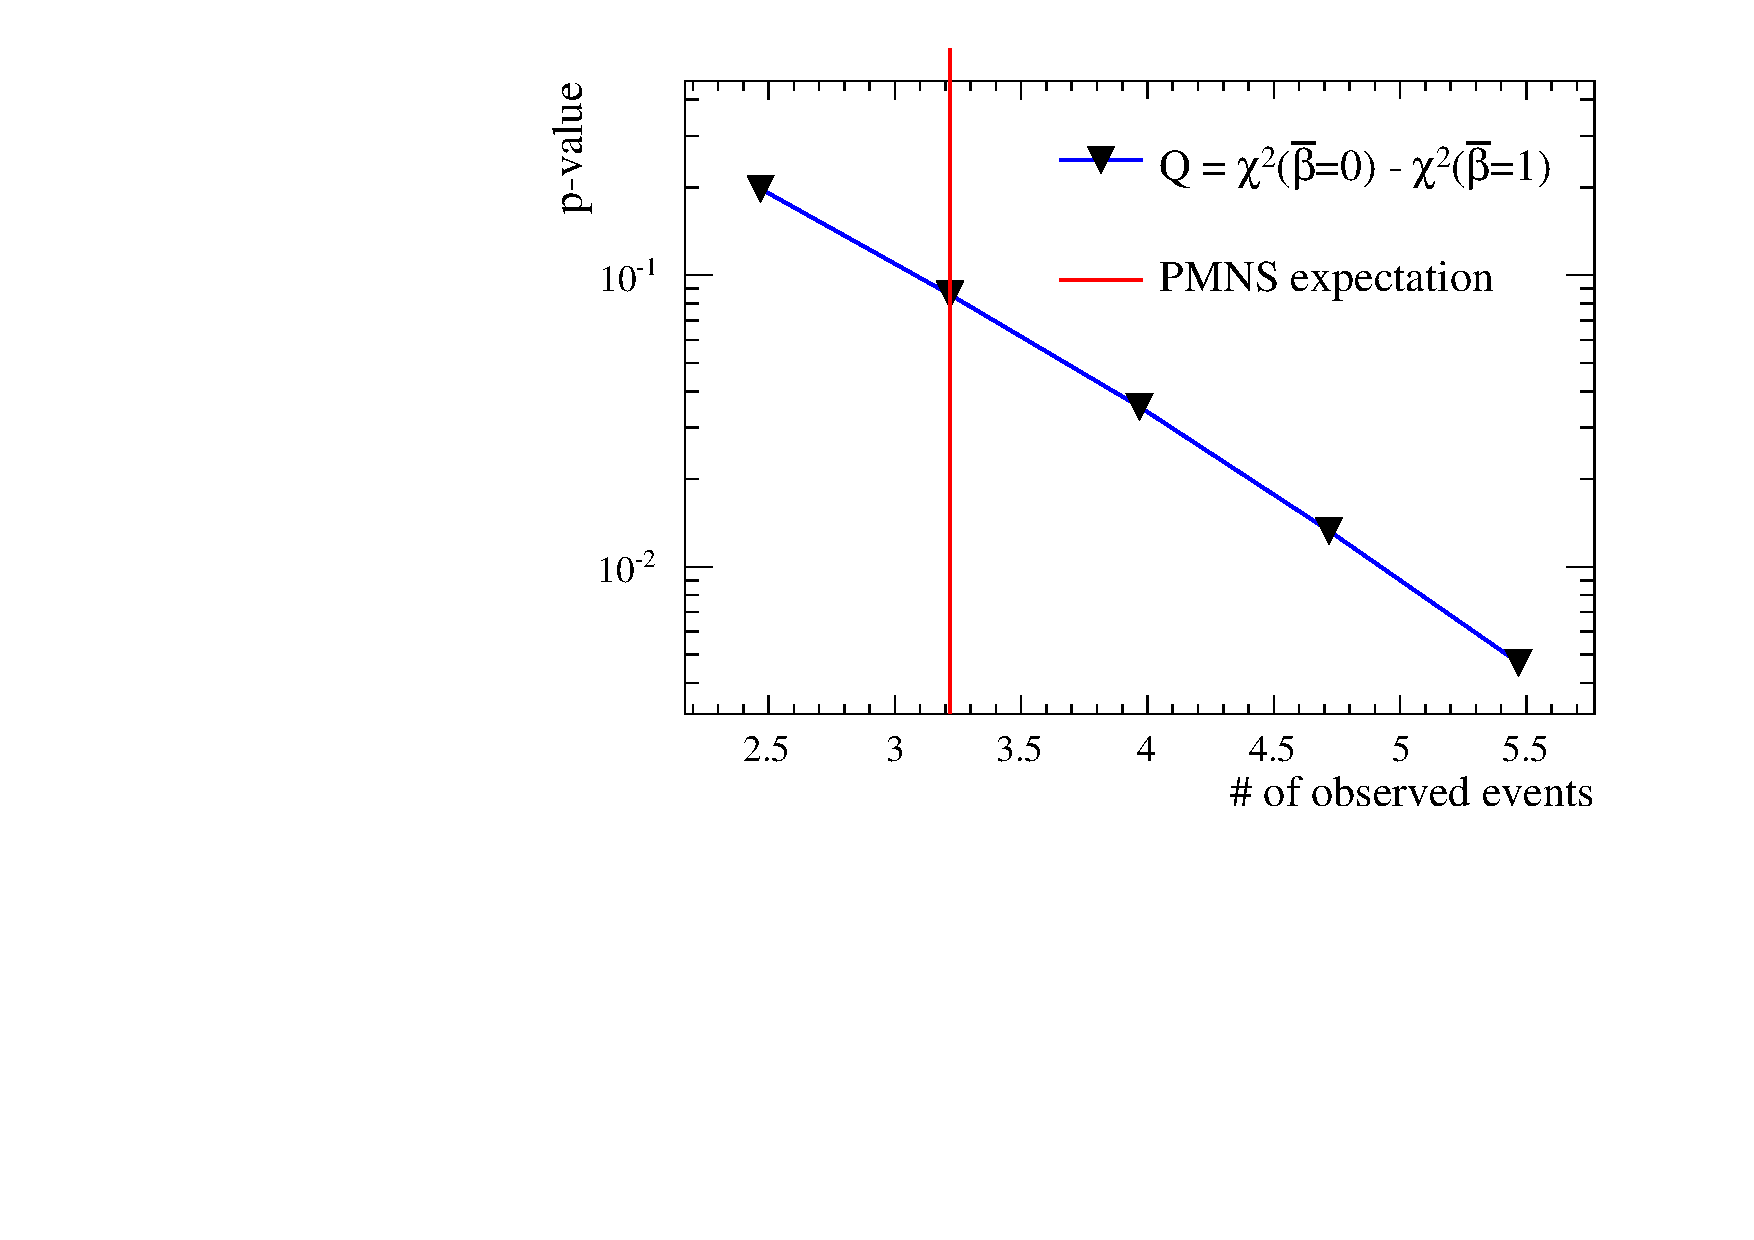
\includegraphics[width=0.9\linewidth]{./joint_plots/nuebar/rateshape/pvalue_Vs_nevt_ratepshape_log.pdf}
\caption{Something else}
\end{subfigure}
\caption {
%{\huge TO UPDATE} 
Rate-only (violet) and rate+shape (blue) p-value given by Asimov datasets for several values of $\beta$
in normal (left) and logarithmic (right) scale.
The red line corresponds to the PMNS expectation ($\beta =1$).
The study is done simulating the Run 1-6 statistic.
\NumToysLarge toys are used.
}
\label{fig:pvalue_Vs_beta_lowpot}
\end{figure}

\begin{figure}
\center
\begin{subfigure}[b]{0.49\textwidth}
\center
%
\includegraphics[width=0.9\textwidth]{./images/missing_plot-eps-converted-to.pdf}
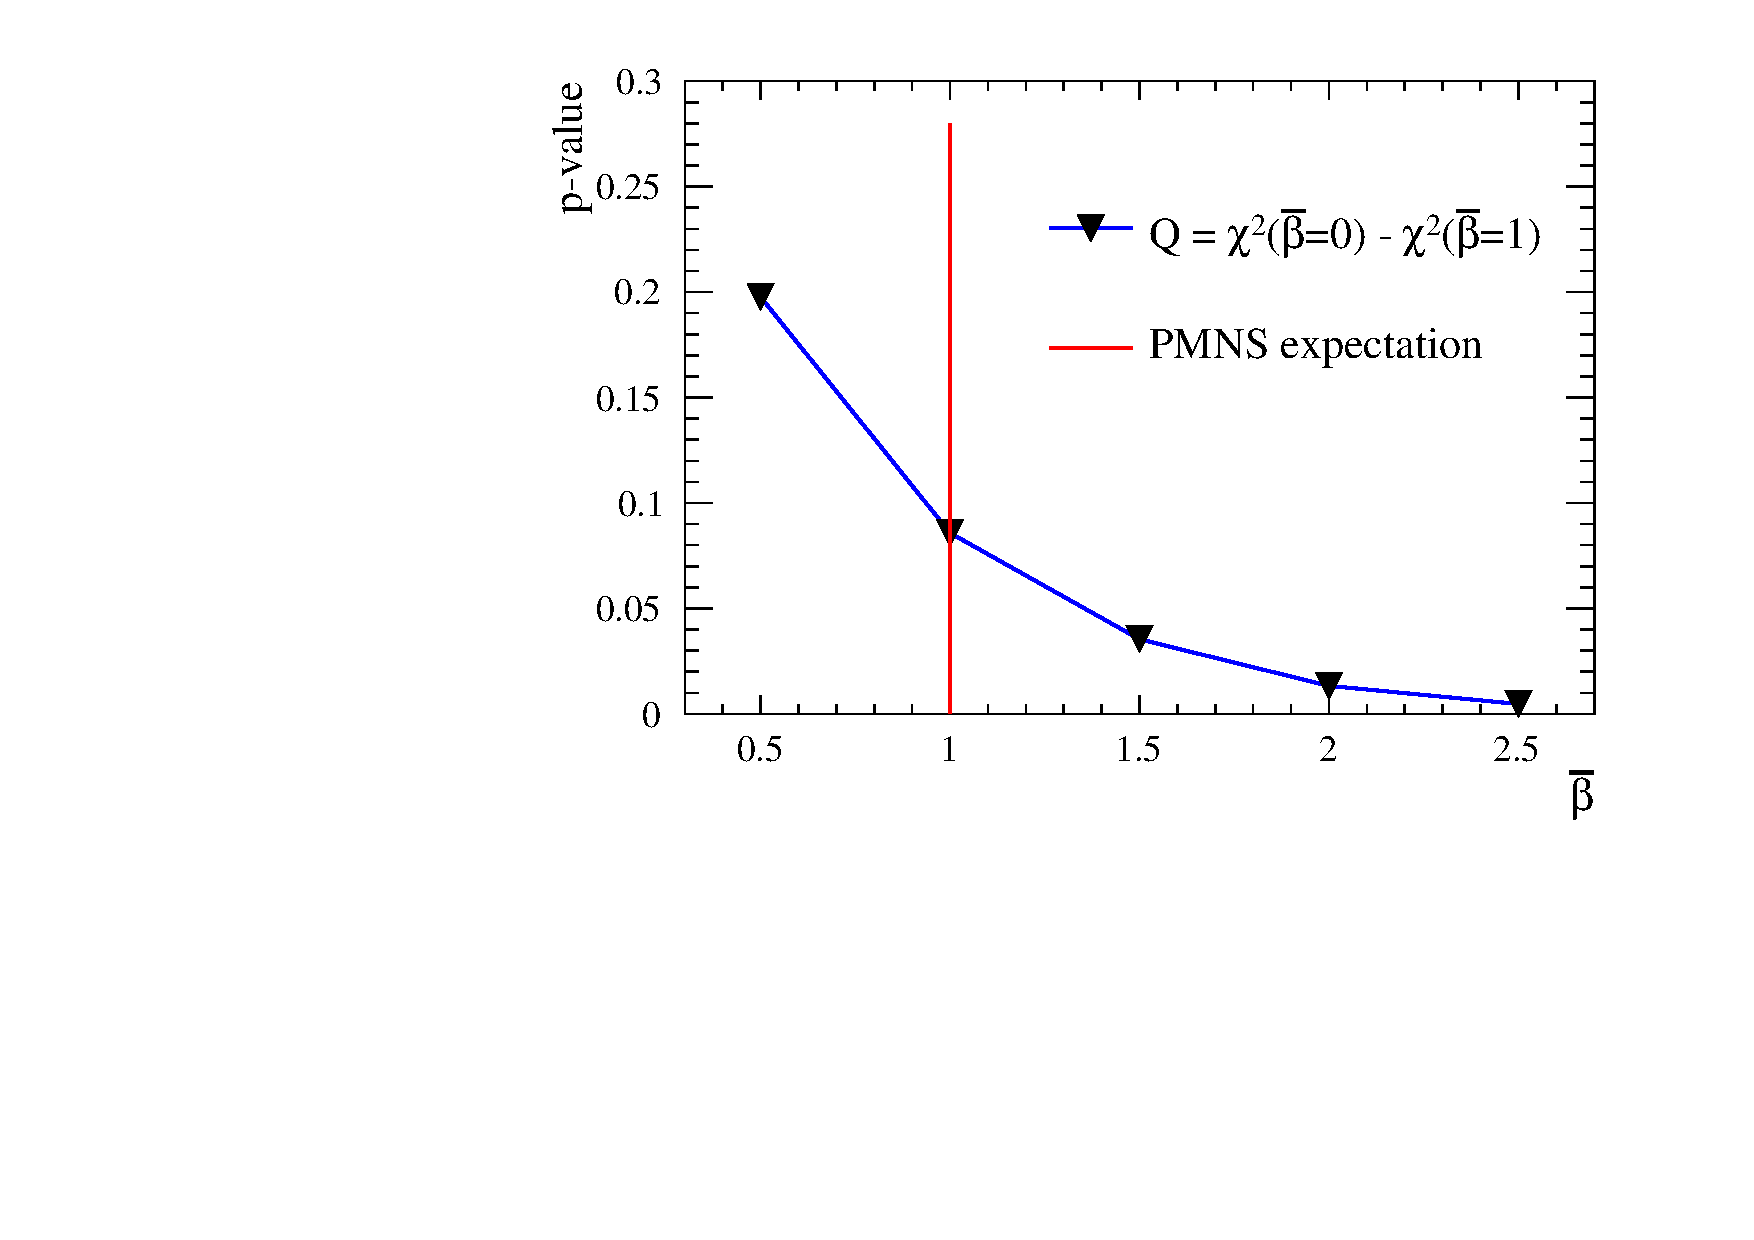
\includegraphics[width=0.9\linewidth]{./joint_plots/nuebar/rateshape/pvalue_Vs_betabar_ratepshape.pdf} 
\caption{Something}
\end{subfigure}
\begin{subfigure}[b]{0.49\textwidth}
\center
%
\includegraphics[width=0.9\textwidth]{./images/missing_plot-eps-converted-to.pdf}
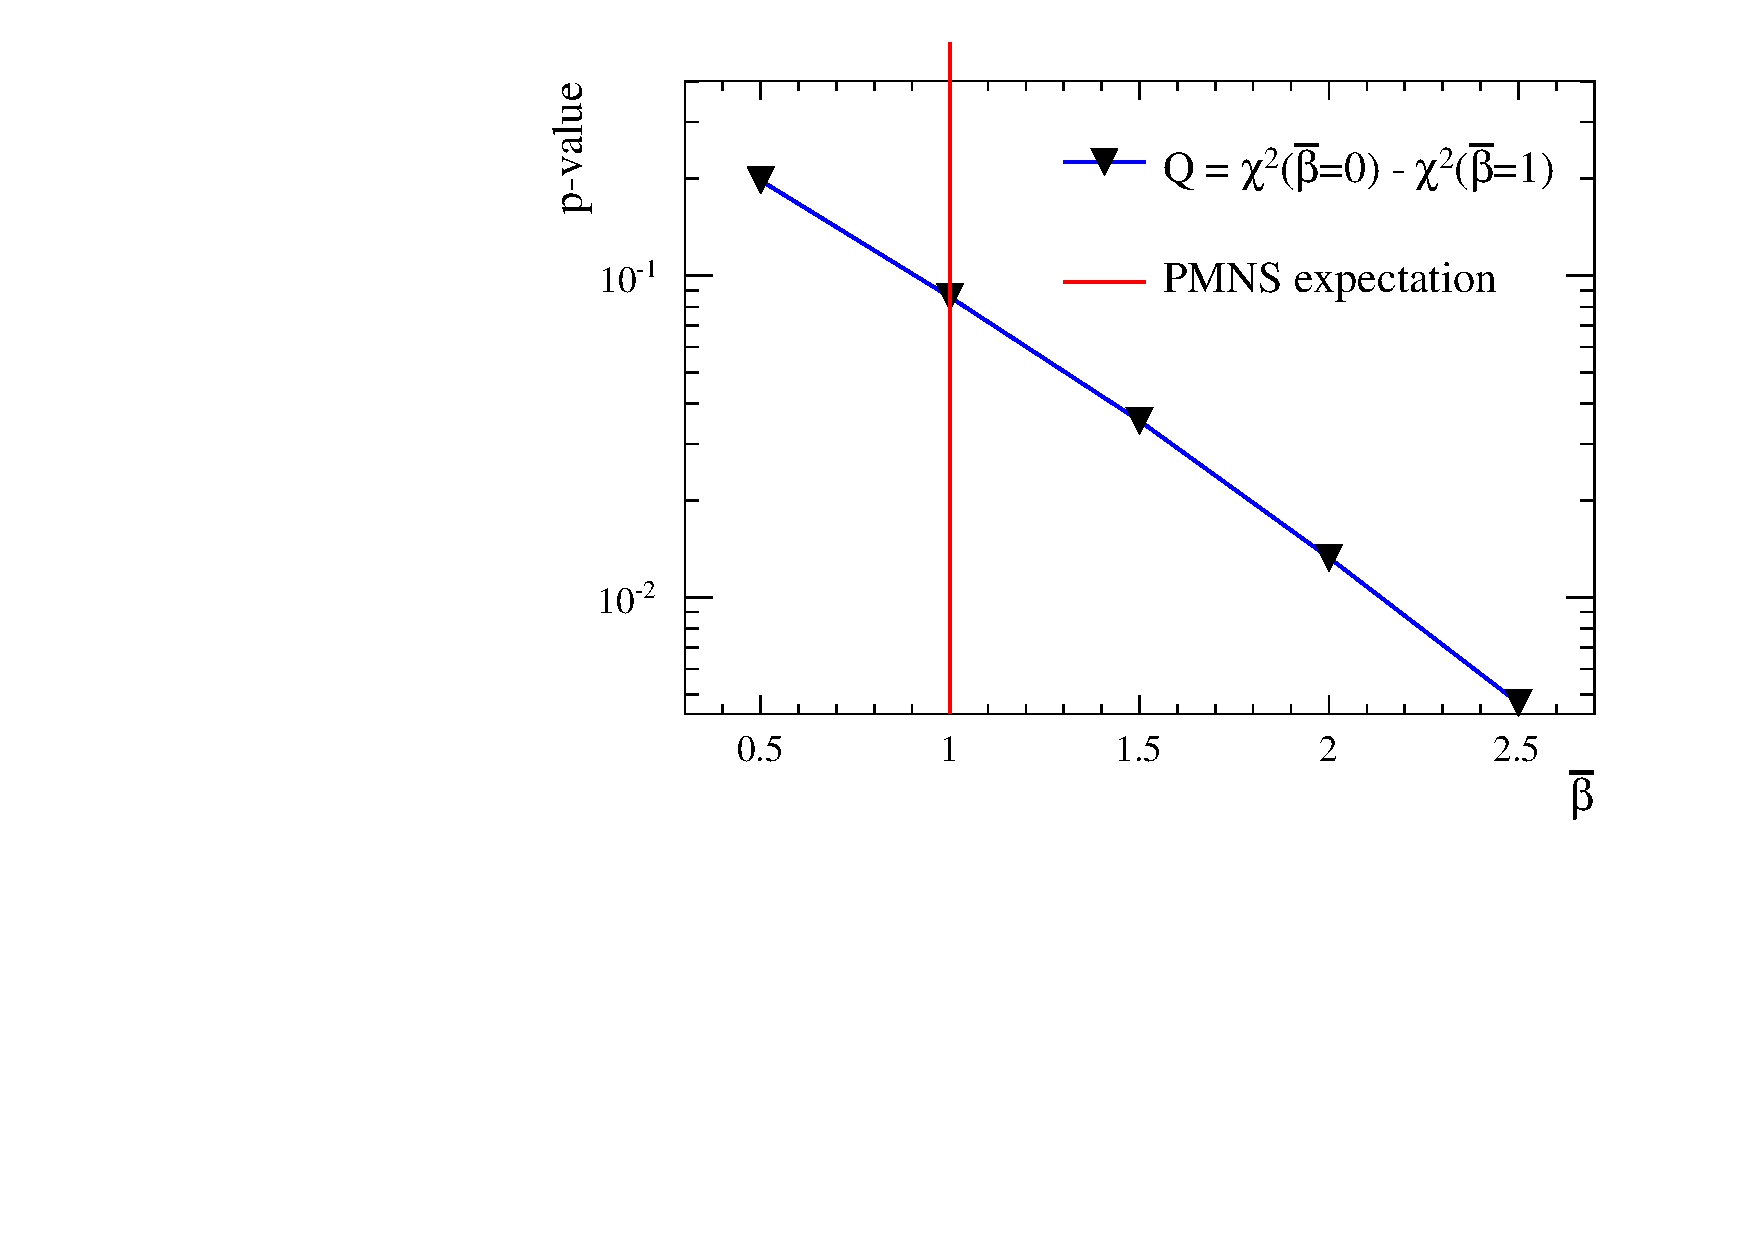
\includegraphics[width=0.9\linewidth]{./joint_plots/nuebar/rateshape/pvalue_Vs_betabar_ratepshape_log.pdf}
\caption{Something else}
\end{subfigure}
 \caption {
%{\huge TO UPDATE} 
Rate-only (violet) and rate+shape (blue) p-value for different number of observed events 
given by Asimov datasets corresponding to the several values of $\beta$ shown in \cref{fig:pvalue_Vs_beta_lowpot}.
Both normal (left) and logarithmic scales (right) are shown.
The red line corresponds to the PMNS expectation ($\beta =1$).
The study is done with Run 1-6 statistic. 
\NumToysLarge toys are used.
}
\label{fig:pvalue_Vs_nevents_lowpot}
\end{figure}


%\begin{figure}
%\center
%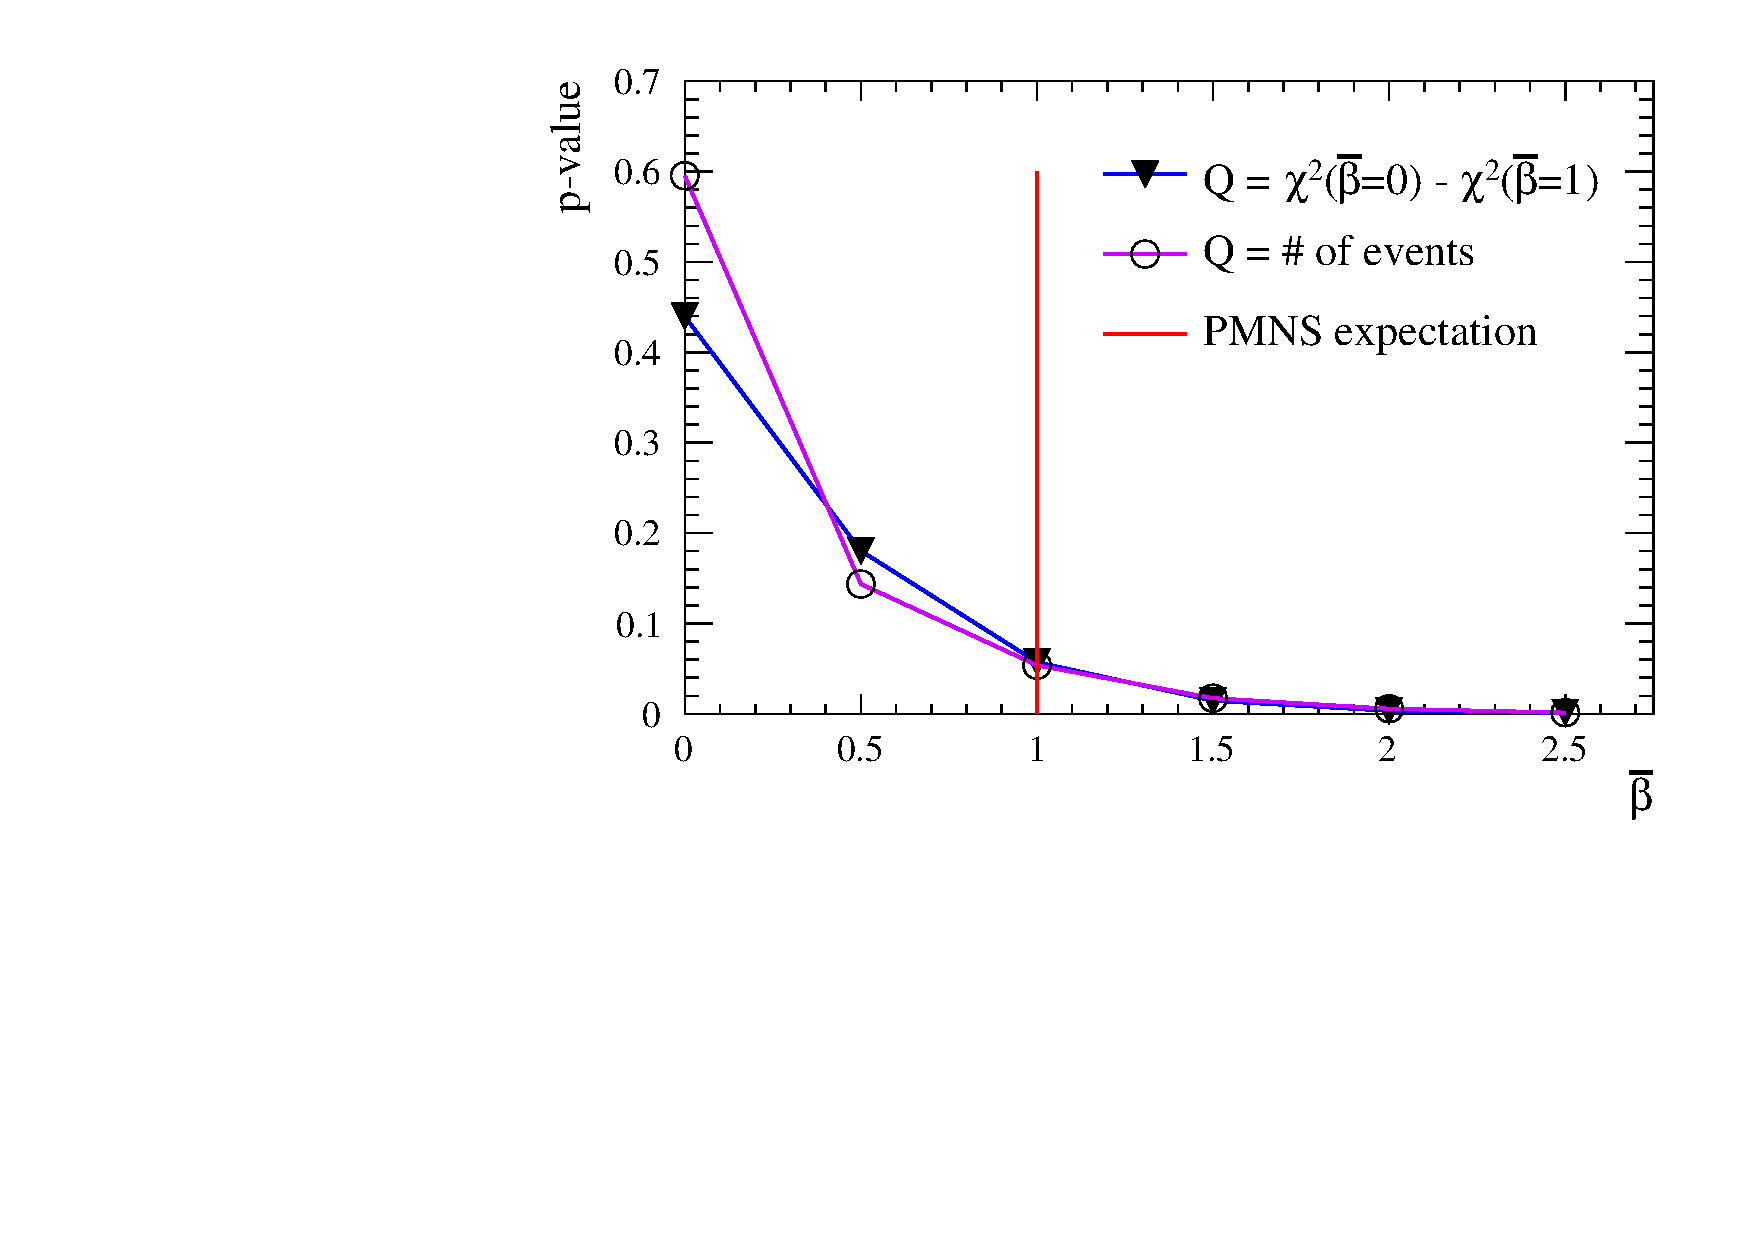
\includegraphics[width=0.48\linewidth]{./nuebar_plots/sensitivity/pvalue_Vs_beta_4p5E20POT.pdf}
%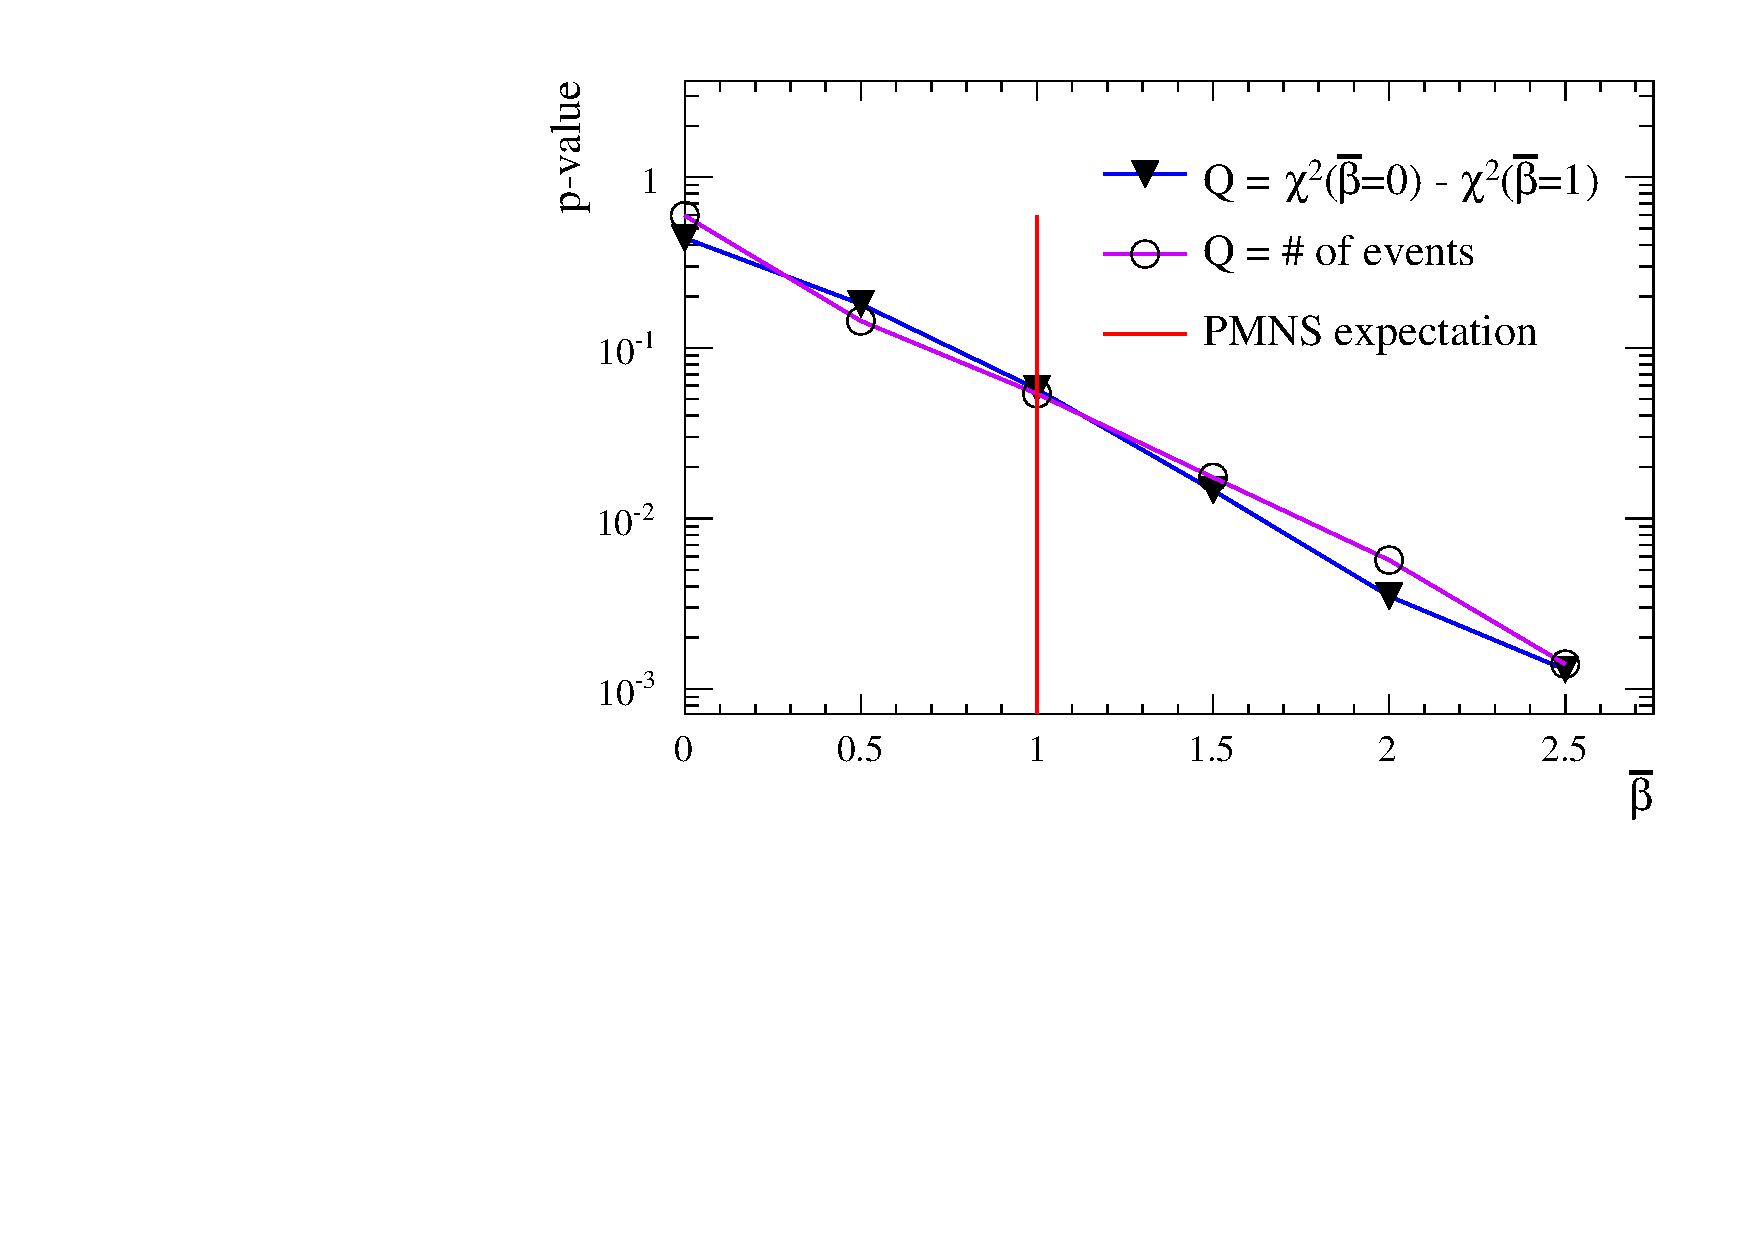
\includegraphics[width=0.48\linewidth]{./nuebar_plots/sensitivity/pvalue_Vs_beta_4p5E20POT_log.pdf}
%\caption {
%Rate-only (violet) and rate+shape (blue) p-value given by Asimov datasets for several values of $\beta$
%in normal (up) and logarithmic (bottom) scale.
%The red line corresponds to the PMNS expectation ($\beta =1$).
%The study is done with 
%\FakePotHigh POT.
%%\newline
%%{\bf TO UPDATE}
%%\newline
%}
%\label{fig:pvalue_Vs_beta_highpot}
%\end{figure}
%
%\begin{figure}
%\center
%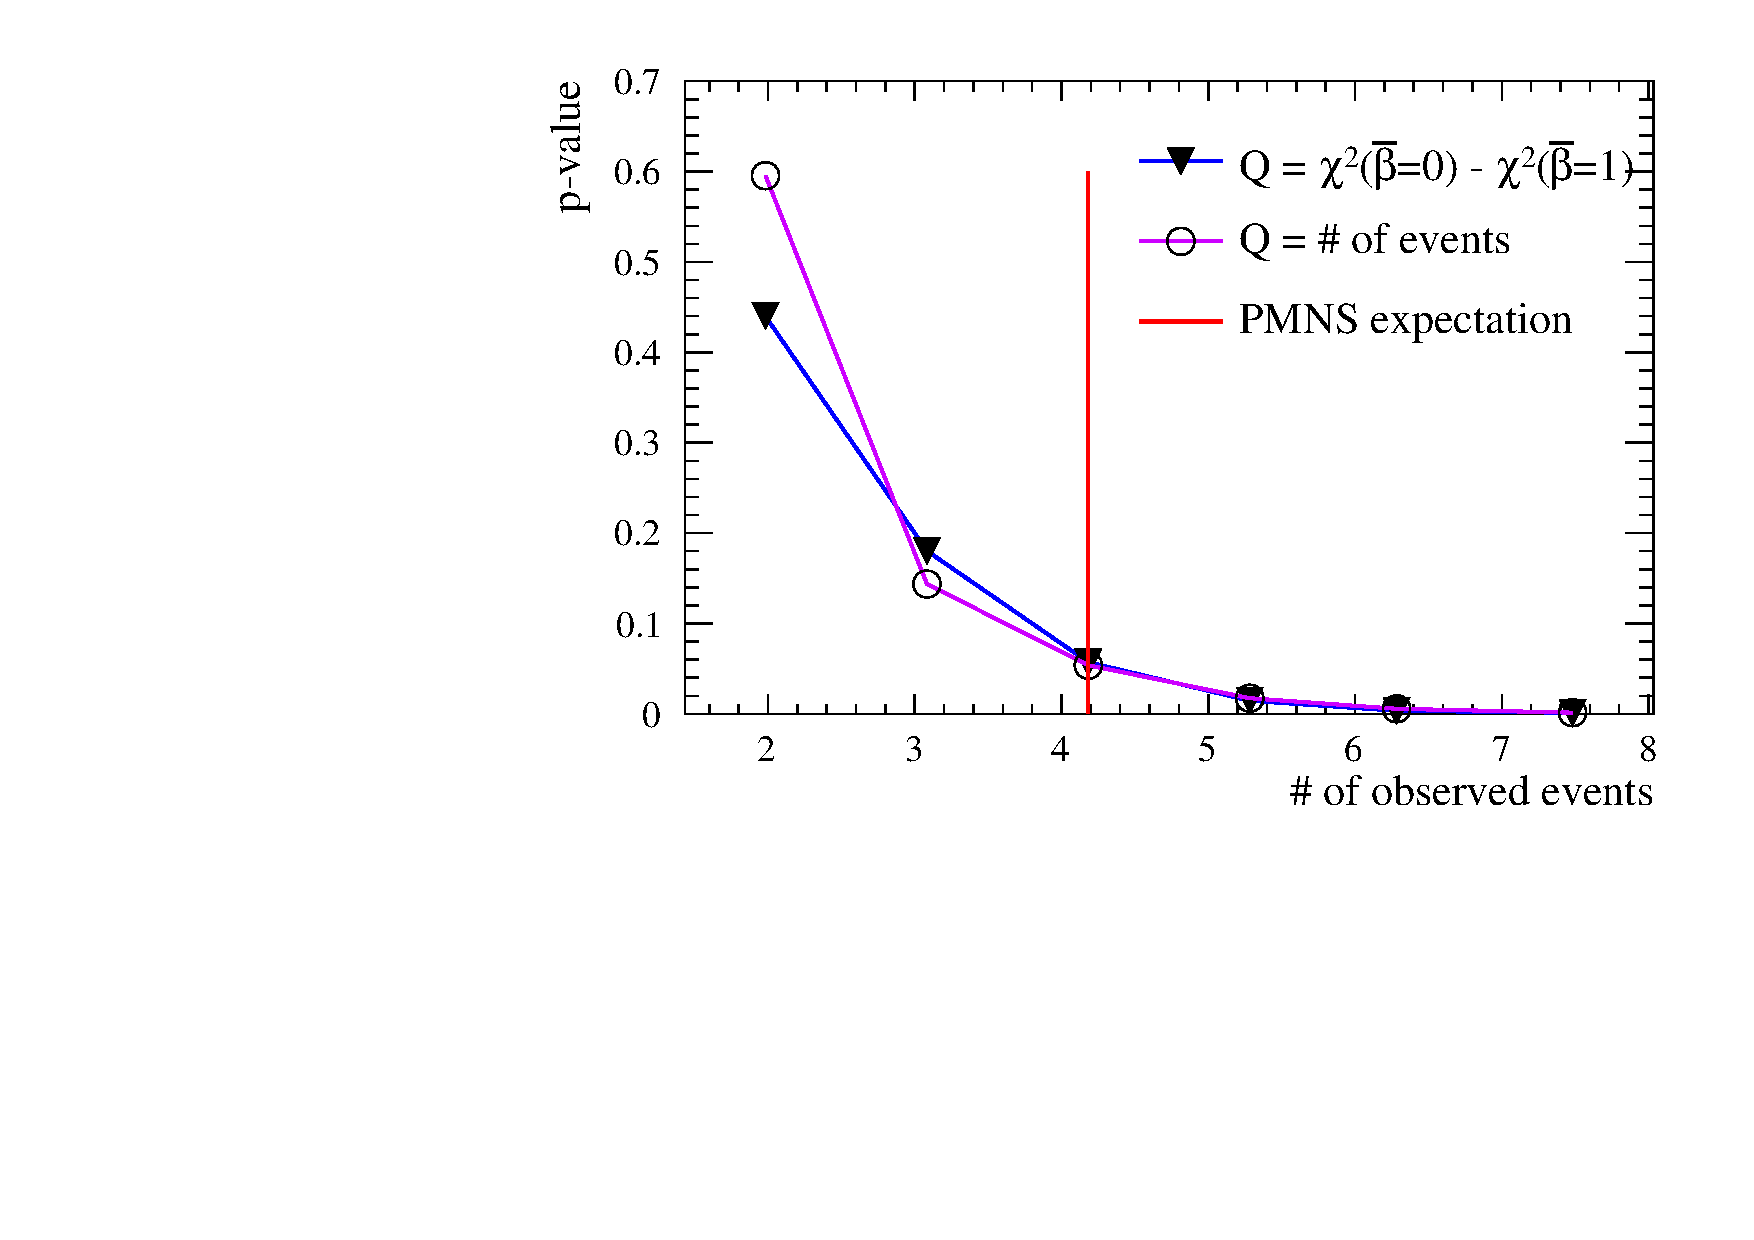
\includegraphics[width=0.48\linewidth]{./nuebar_plots/sensitivity/pvalue_Vs_nevents_4p5E20POT.pdf}
%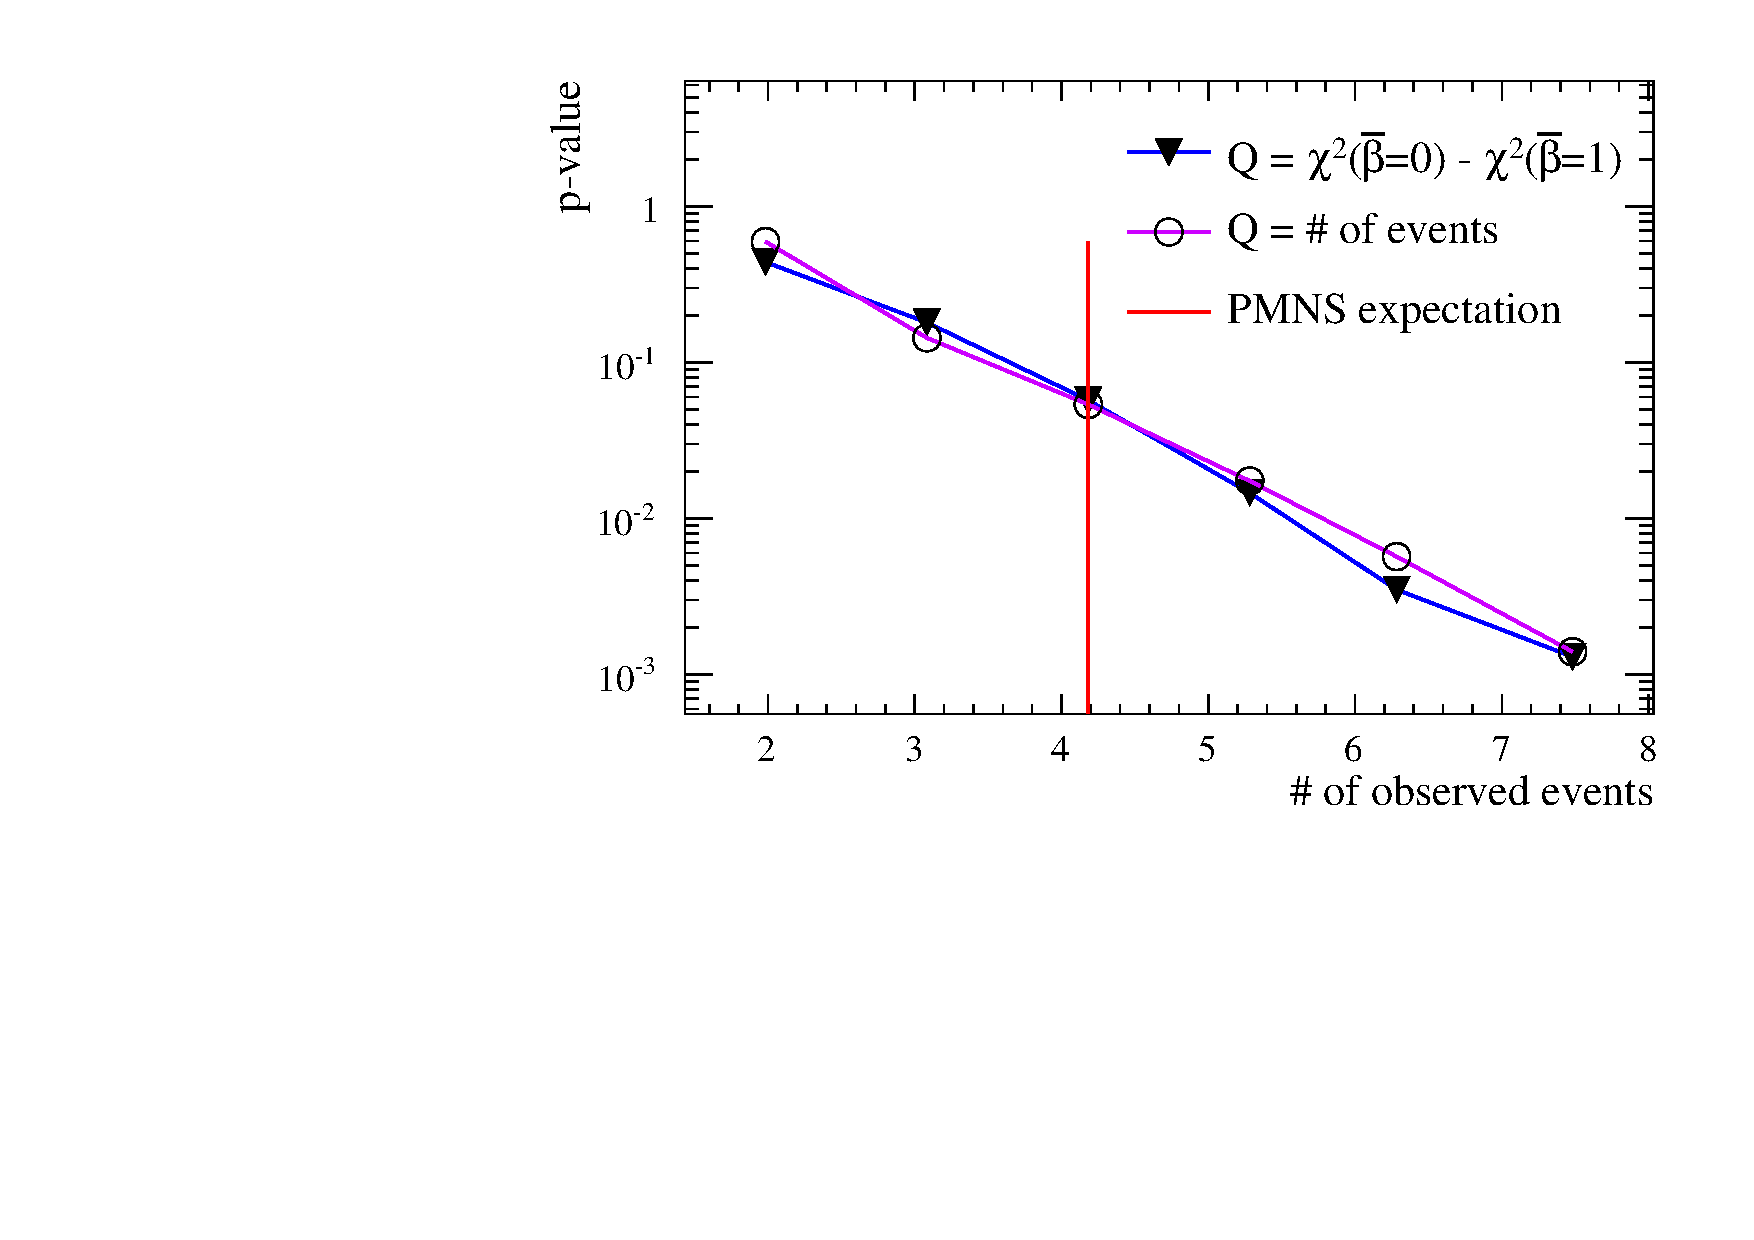
\includegraphics[width=0.48\linewidth]{./nuebar_plots/sensitivity/pvalue_Vs_nevents_4p5E20POT_log.pdf}
%\caption {
%Rate-only (violet) and rate+shape (blue) p-value for different number of observed events 
%given by Asimov datasets corresponding to the several values of $\beta$ shown in \cref{fig:pvalue_Vs_beta_highpot}.
%Both normal (up) and logarithmic scales (bottom) are shown.
%The red line corresponds to the PMNS expectation ($\beta =1$).
%The study is done with 
%\FakePotHigh POT.
%%\newline
%%{\bf TO UPDATE}
%%\newline
%}
%\label{fig:pvalue_Vs_nevents_highpot}
%\end{figure}


%--------------------------------------------------------------------------------------------------------------------

\subsection {Mean p-value}
\label{subsec:pvalue_mean}

The mean p-value is computed without using the Asimov dataset, but with toy experiments:
\begin{itemize}
\item the distributions shown in \cref{fig:pvalue_rateonly} and \cref{fig:pvalue_rateshape} 
	are used respectively for the rate-only and rate+shape p-value computations,
\item \NumToysLarge toys are produced with $\beta = 1$, 
\item for each toy with $\beta=1$ the test statistic (i.e. the number of events and 
	$\Delta \chi^2$ given in \cref{eq:deltachisq_rateshape})
	is computed and a 1-sided p-value (right tail) is quoted using the distributions 
	\cref{fig:pvalue_rateonly} and \cref{fig:pvalue_rateshape}, 
\item a distribution of rate-only and rate+shape p-values is obtained and the mean p-value is calculated.
\end{itemize}

The mean rate-only p-value, given by the mean of the p-value distribution shown in \cref{fig:pvalue_mean}, is XXX
while the mean rate+shape p-value is 0.170 for 
Run 1-6 statistic.
%\TotalPot POT.
%\FakePotLow POT.
%For \FakePotHigh POT the rate-only p-value is 0.188 while the rate+shape is 0.127.
%For both cases 
The mean p-value is larger than the Asimov one, which corresponds to the most probable p-value. 
It is worth to point out that sometimes it can happen that the rate-only
p-value is smaller than the rate+shape one. This can be due to both the discreteness of the rate-only
p-value or to the shape information wich can discard the $\bar{\nu}_e$ appearance hypothesis.
On average the rate+shape p-value is smaller than the rate-only one,
since it exploits also the shape information, but if a single dataset is used
it can happen that, due to the discreteness of test statistic (number of events), the rate-only p-value
is smaller than the rate+shape p-value.
Indeed a change of the number of events produce a not small jump in the p-value, 
as shown in the left plot of \cref{fig:pvalue_mean}, while the distribution of the 
rate+shape p-value is smooth and continuos.
For this reason it is important to quote both the p-values.
 
\begin{figure}
\center
%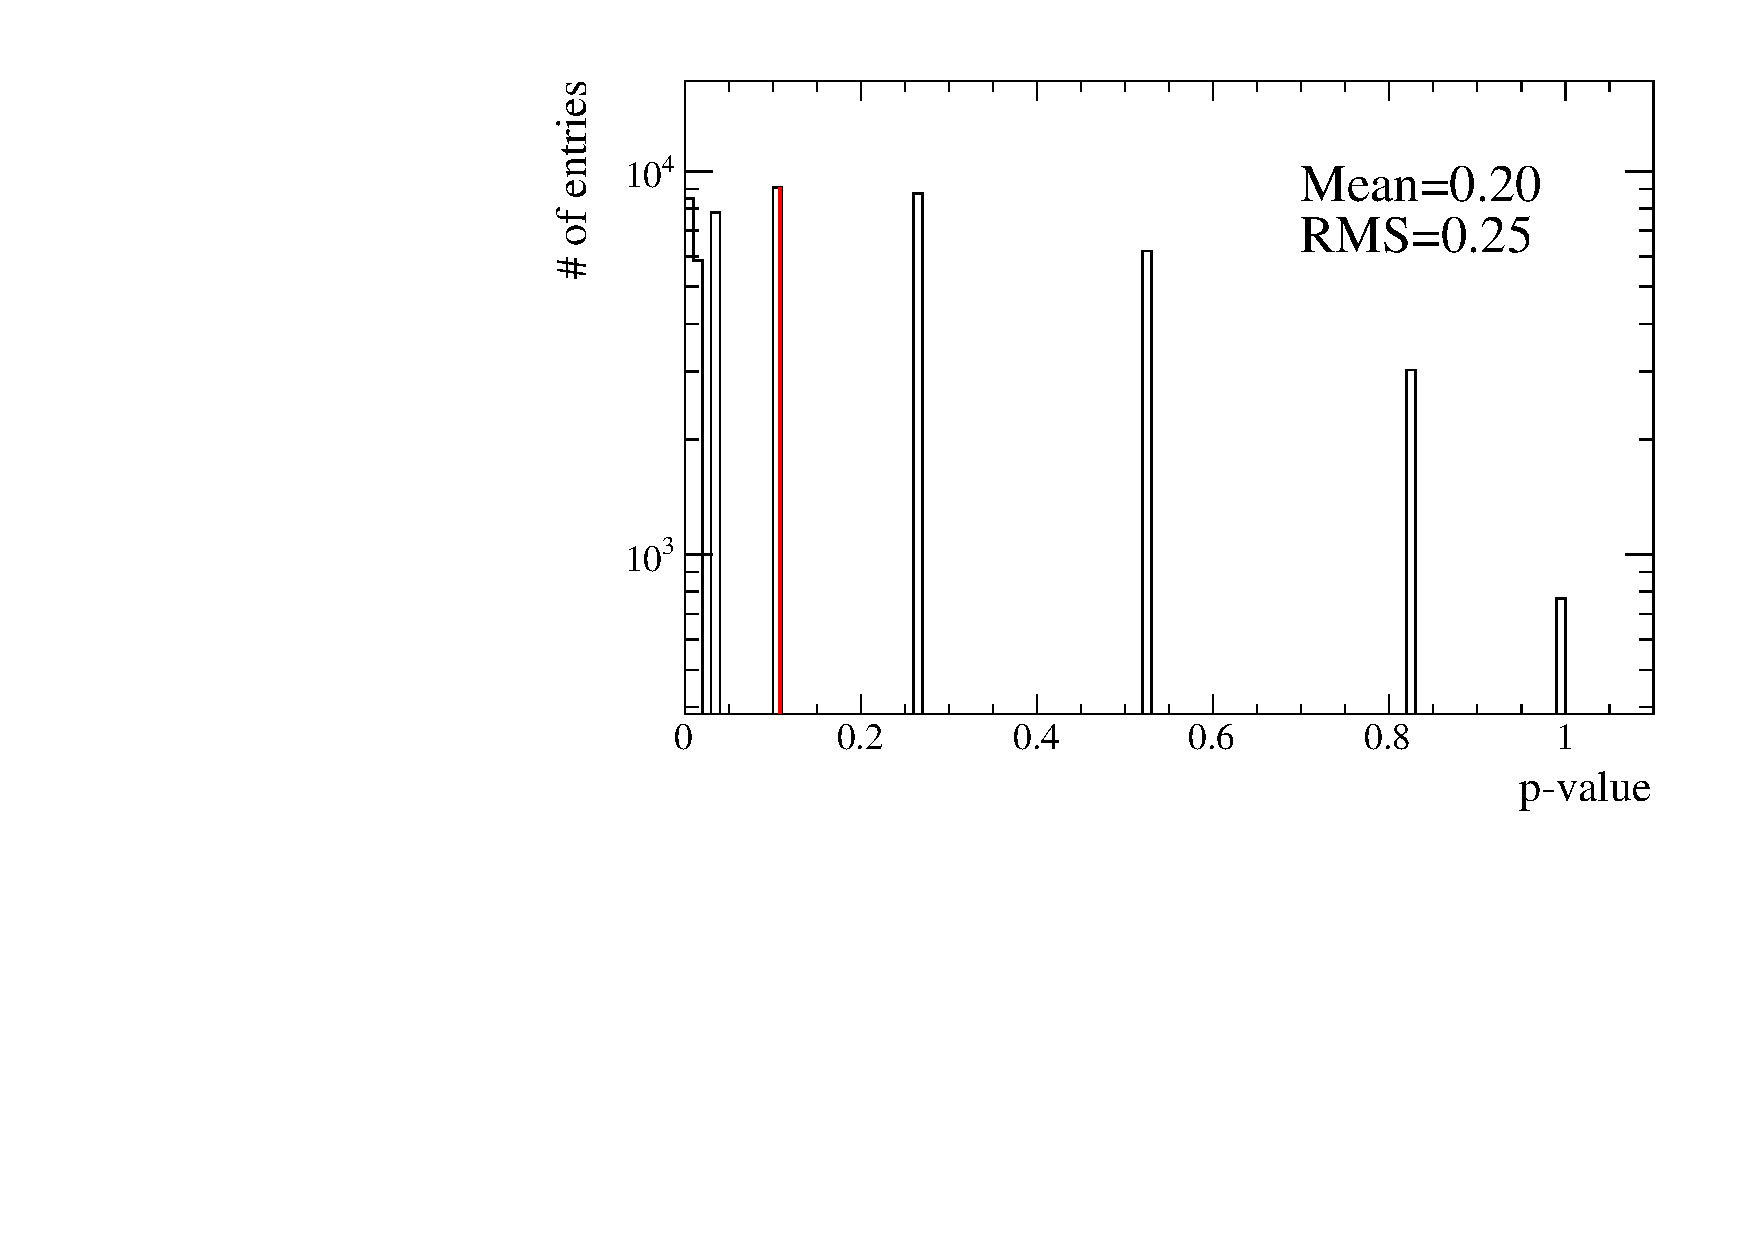
\includegraphics[width=0.48\linewidth]{./nuebar_plots/pvalue_mean/pvalue_rateonly_ave_all_4p0108E20POT_50ktoys.pdf}
\begin{subfigure}[b]{0.49\textwidth}
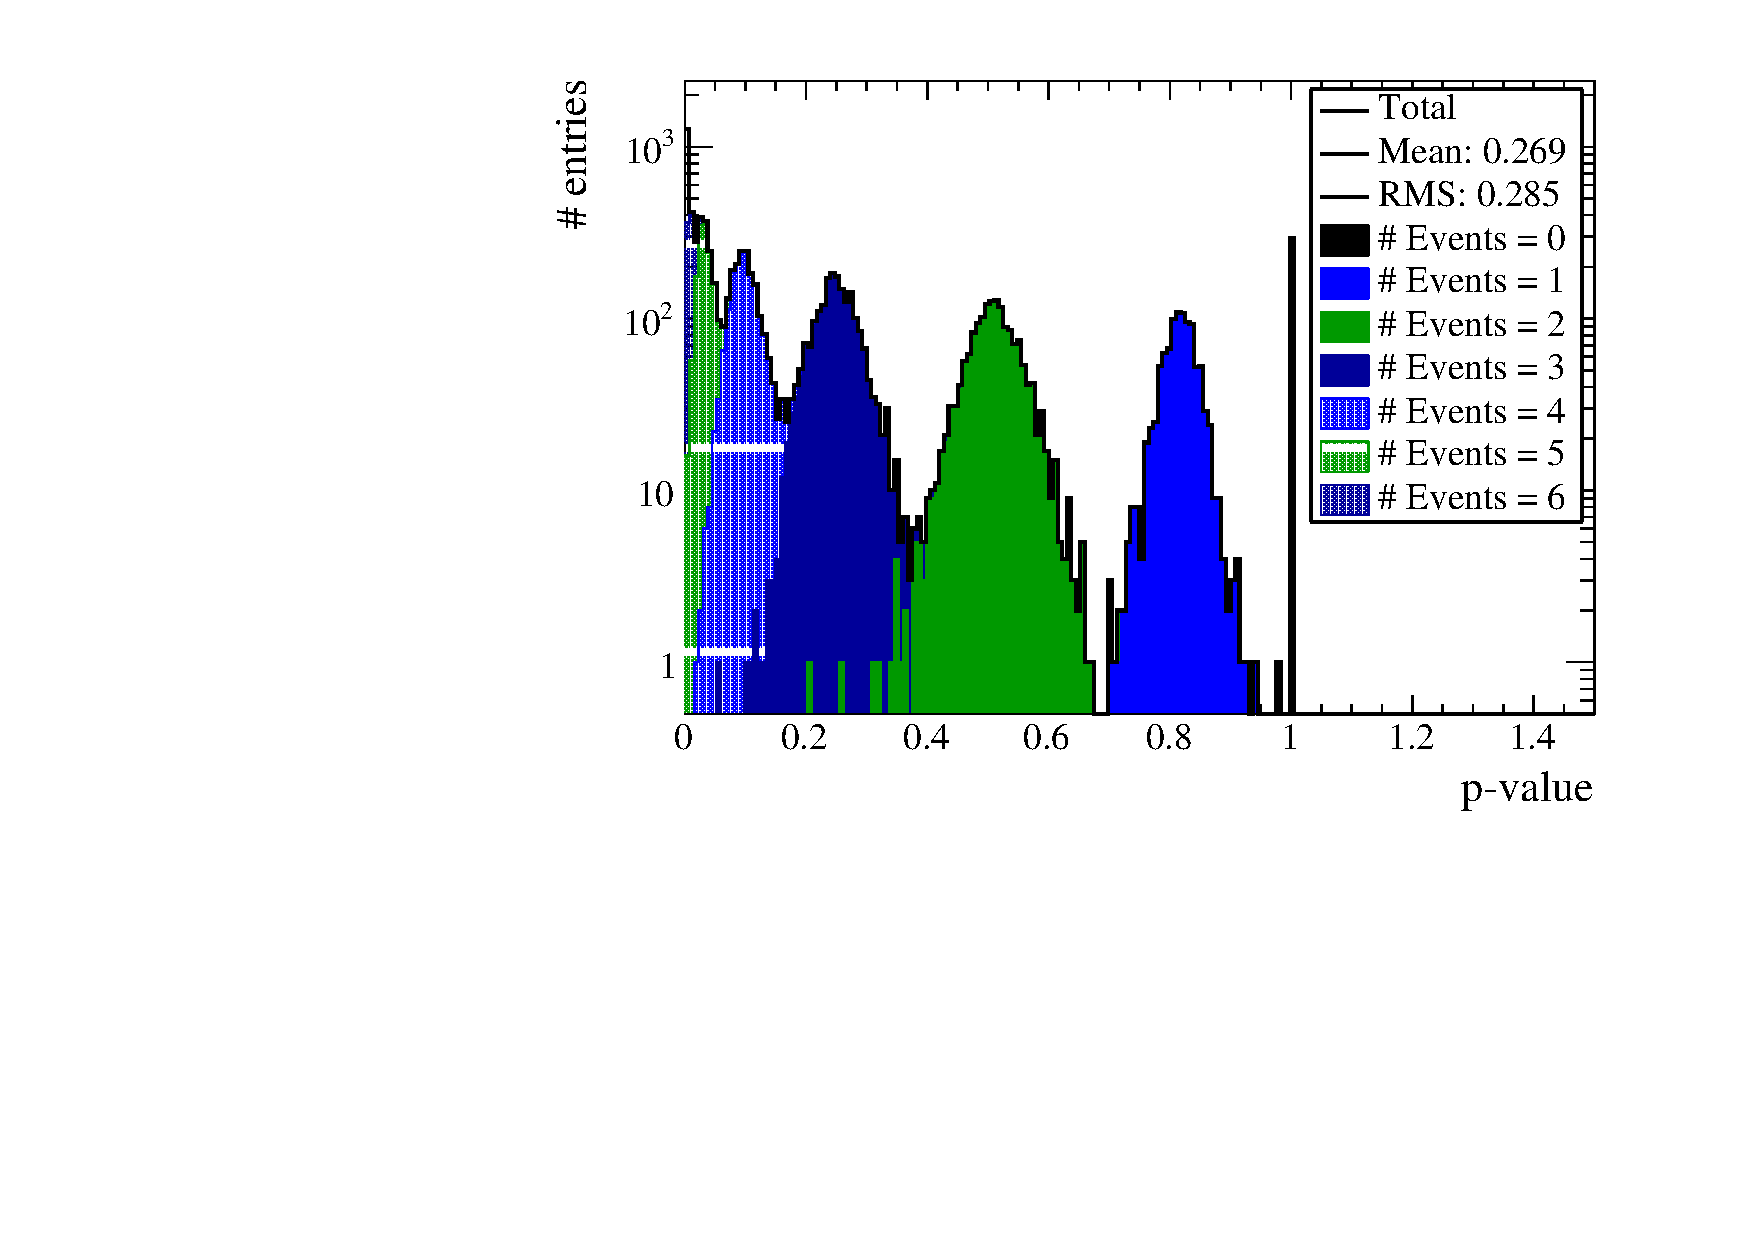
\includegraphics[width=0.9\textwidth]{./joint_plots/nuebar/rateonly/pvalue_data_beta1_dist_0.pdf}
\caption{Rate only}
\end{subfigure}
\begin{subfigure}[b]{0.49\textwidth}
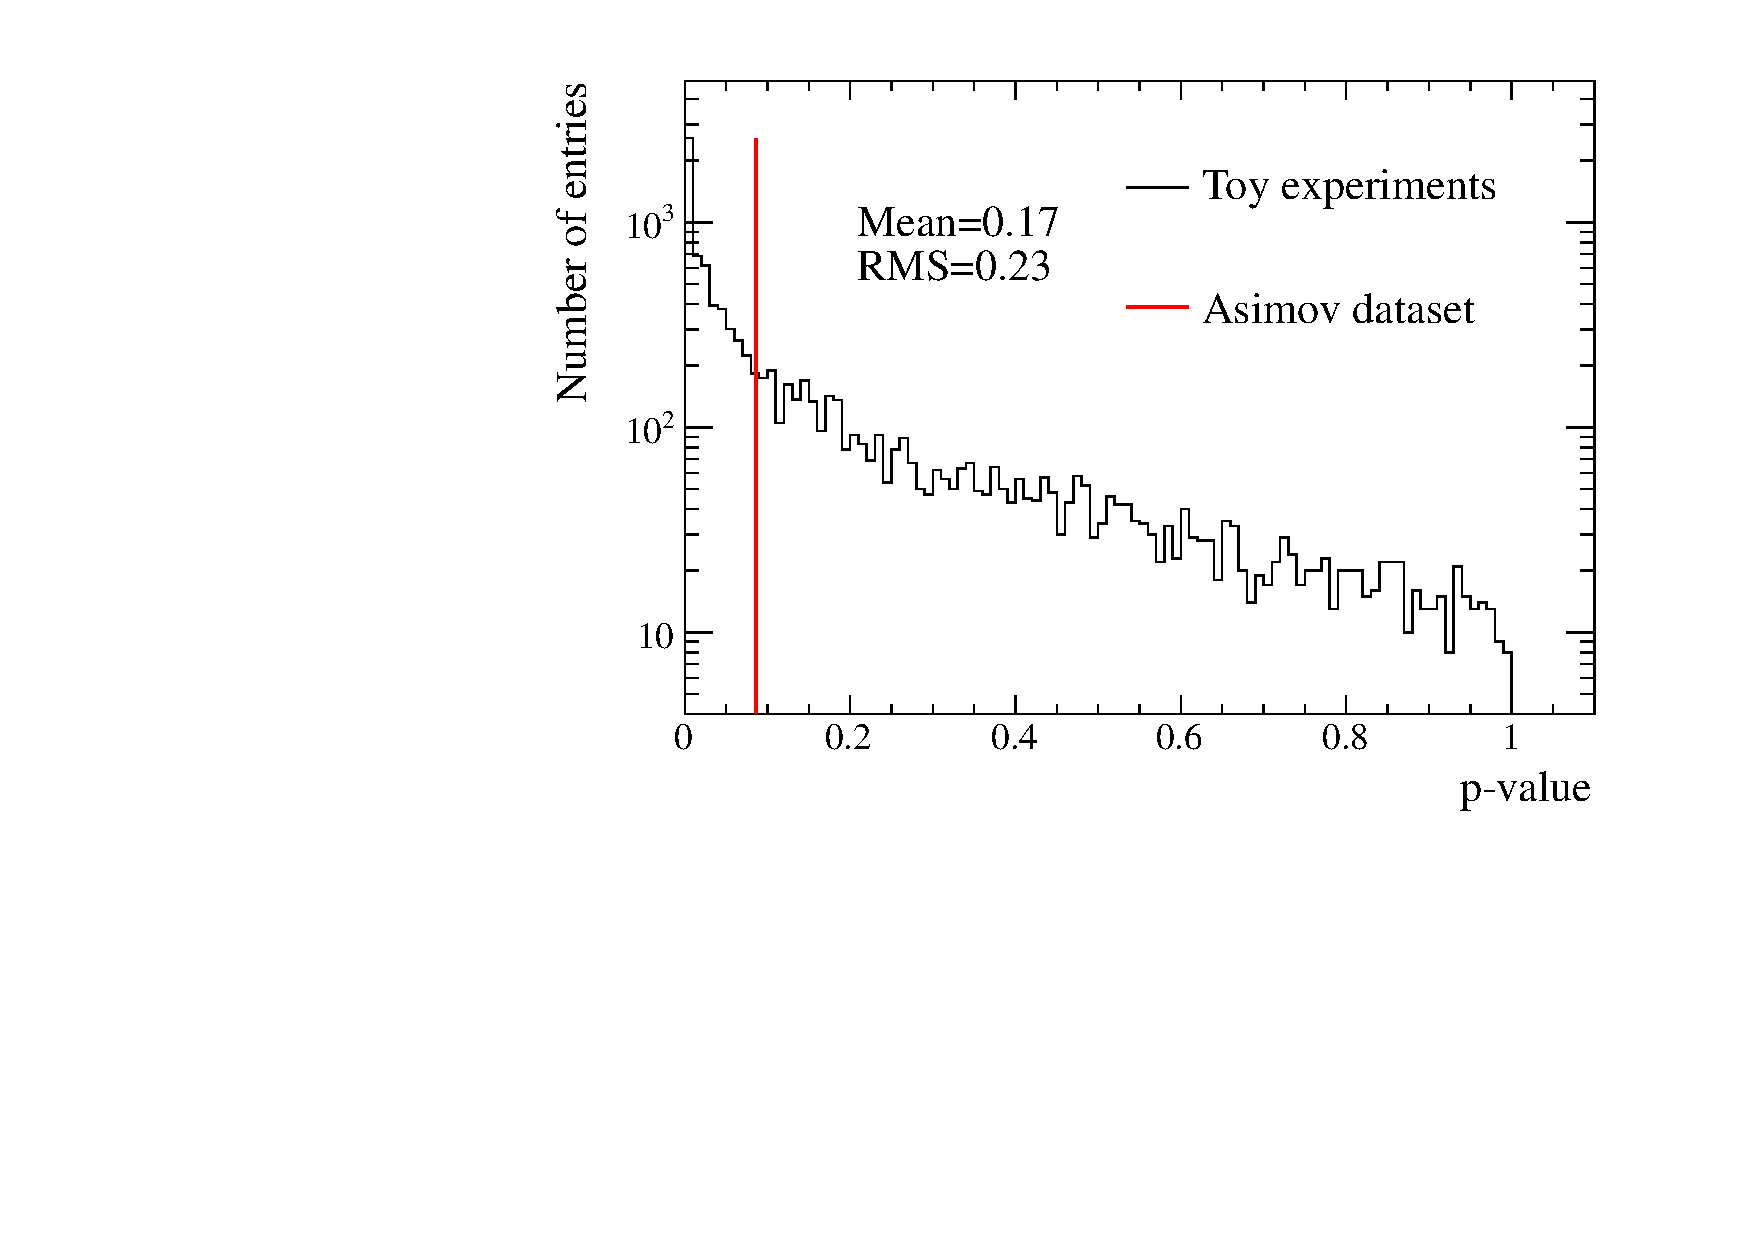
\includegraphics[width=0.9\textwidth]{./joint_plots/nuebar/rateshape/cPvalue_rateshape.pdf}
\caption{Rate + Shape}
\end{subfigure}
\caption {
%{\huge TO UPDATE} 
Distribution p-values obtained by \NumToysLarge toys with $\beta=1$.
The rate-only p-value is discrete and each filled bin correspond to toys with different number of events.
In both distributions the spike at p-value=1 corresponds to toys with no events.
The study is performed with 
Run 1-6 statistic.
\NumToysLarge toys are used.
}
\label{fig:pvalue_mean}
\end{figure}

In \cref{fig:pvalue_Vs_nevents_2Dplot} the rate+shape p-value as a function 
of the number of events for single toy produced with $\beta=1$ is shown for the Run 1-6 statistic.

\begin{figure}
\center
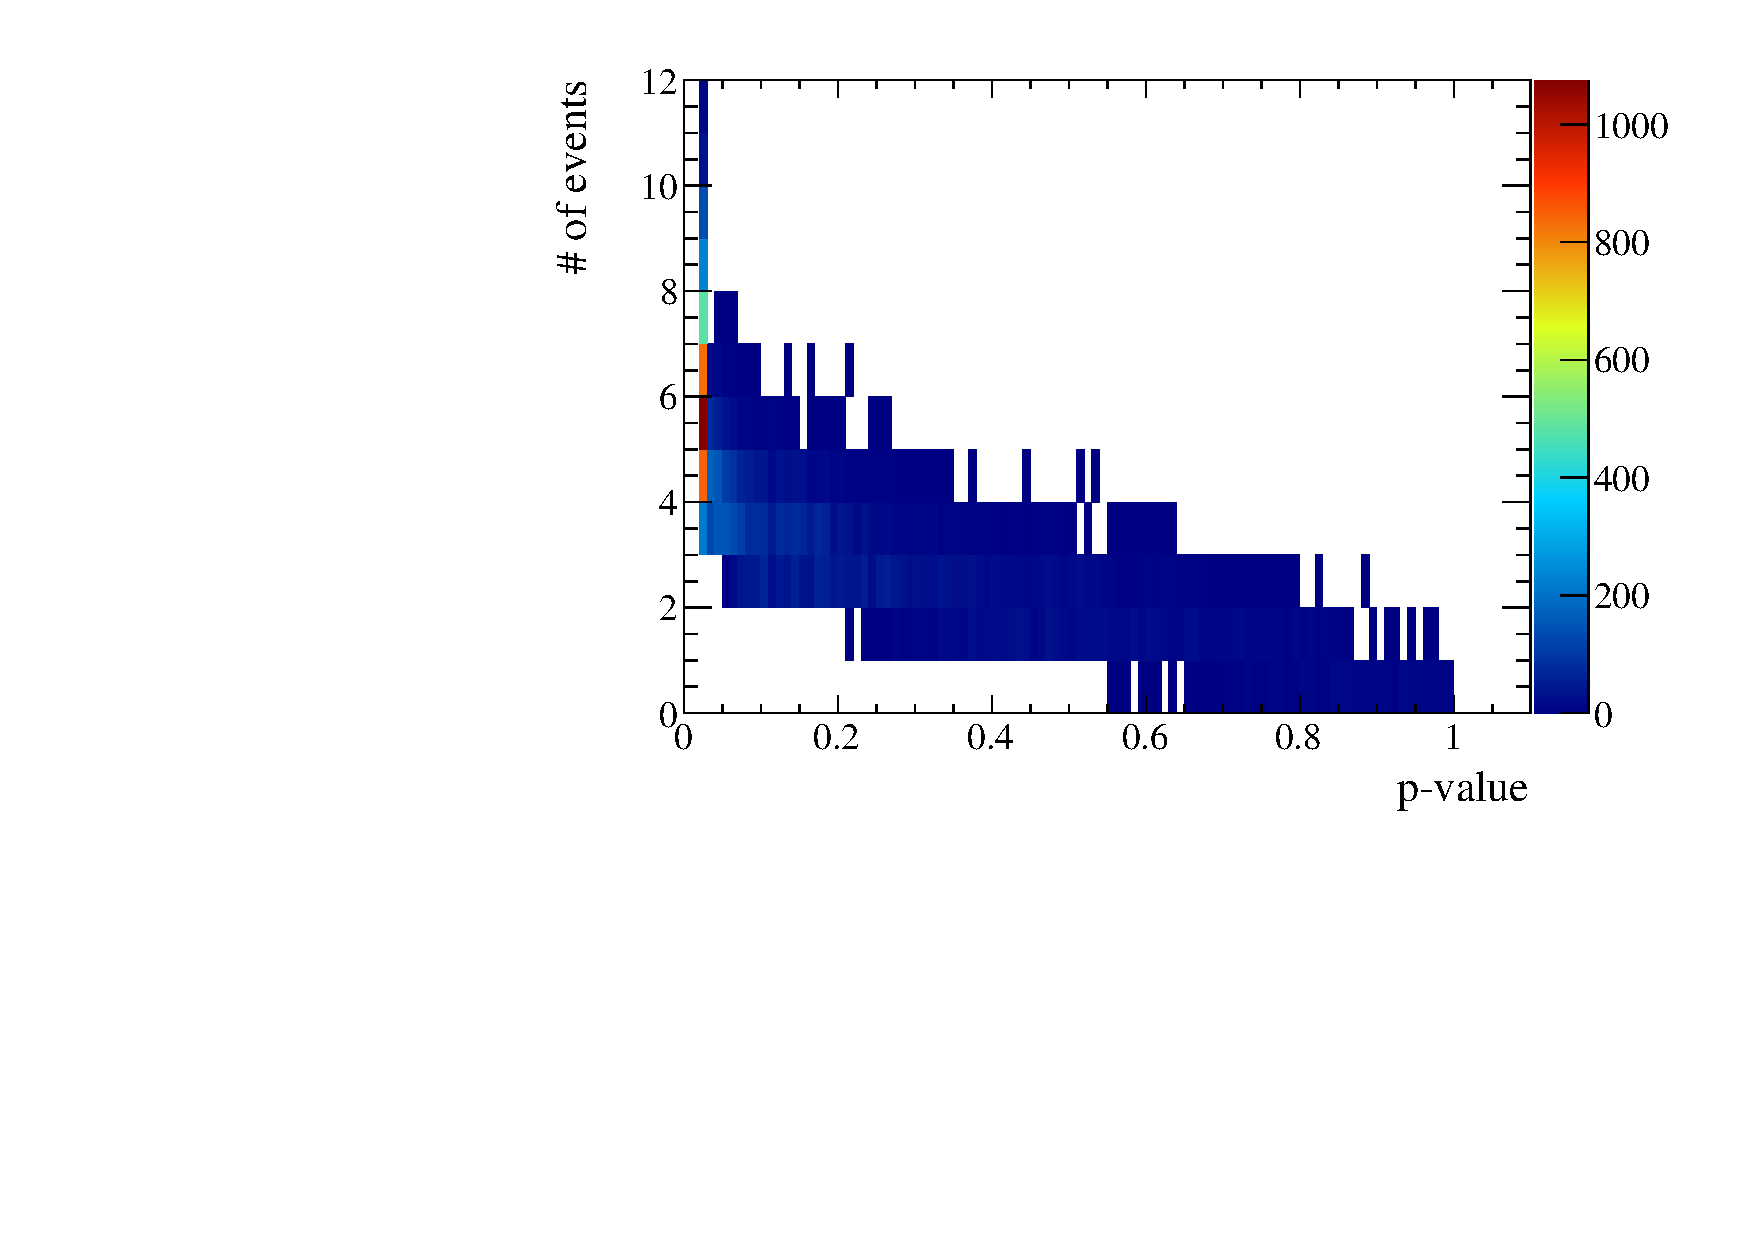
\includegraphics[width=0.6\linewidth]{./joint_plots/nuebar/rateshape/cPvalueVsNevt.pdf}
\caption {
The rate+shape p-value as a function of the number of events for a single toy produced with $\beta=1$ is shown for 
the Run 1-6 statistic.
\NumToysLarge toys are produced as described in \cref{subsec:pvalue_mean}. 
Each entry corresponds to a different toy. 
}
\label{fig:pvalue_Vs_nevents_2Dplot}
\end{figure}


%--------------------------------------------------------------------------------------------------------------------

\subsection {Summary of expected significance to $\bar{\nu}_e$ appearance}
\label{subsec:summary_sensi}

In \cref{tab:summary_sensi_lowpot} 
the expected rate-only and rate+shape p-values corresponding 
to 
Run 1-6 statistic.
In \cref{tab:summary_sensi_rateonly}
the expected rate-only p-value is shown for different number of observed events
for
Run 1-6 statistic.

%In \cref{tab:summary_sensi_manytoys_4p0108E20POT} and \cref{tab:summary_sensi_manytoys_8E20POT}
%the Asimov and Mean p-values are shown for both 
%Run 1-6 statistic 
%and $8\times 10^{20}$ POT.
%It can be seen that the expected p-value is very close to the one computed with \NumToysLarge toys.



\begin{table}
\centering
\begin{tabular}{| c | c | c |}
\hline
\# of observed events	                        	& Rate only      & Rate + Shape		    	\\
\hline
$N_{obs} = 2$      		                    	& 0.510          &          	\\
$ N_{obs} = 3$      		                    	& 0.251          &          	\\
$ \bf N_{obs} = 4$      		           	         & \bf 0.101     &             \\
$N_{obs} = 5$      		                    	& 0.0343        &        	\\
$N_{obs} = 6$      		                    	& 0.0103        &        	\\
\hline
\end{tabular}
\caption{
Summary of the expected rate-only p-values for different number of 
observed events. The simulated number of POT corresponds to Run 1-6.
\NumToysLarge toys are used to get the distribution of the test statistic and the 
Asimov data is used to compute the p-value.
The Asimov dataset for $\beta=1$ is in bold.
}
\label{tab:summary_sensi_rateonly}
\end{table}




\begin{table}
\centering
\begin{tabular}{| c | c | c |}
\hline
P-value	                                          	& Asimov    	& Mean 		    	\\
\hline
Rate-only                          			& 0.109           	& 0.269                  	\\
Rate+shape                          		& 0.0858          	& 0.170                 	\\
\hline
\end{tabular}
\caption{
Summary of the expected rate-only and rate+shape p-values for 
the Run 1-6 statistic.
The Asimov p-value is calculated using the Asimov dataset while the 
mean p-value is calculated making \NumToysLarge toys and taking the mean 
of the p-value distribution.
}
\label{tab:summary_sensi_lowpot}
\end{table}




%% Comparison with many toys
%
%\begin{table}
%\centering
%\begin{tabular}{| c | c | c |}
%\hline
%P-value	                                          			& Asimov    	  & Mean 		    	\\
%\hline
%Rate-only (\NumToys toys)         			& 0.110           & 0.207                  	\\
%Rate+shape (\NumToys toys)              		& 0.0726          & 0.143                  	\\
%\hline
%Rate-only (\NumToysLarge toys)        		& 0.109           & 0.203                	\\
%Rate+shape (\NumToysLarge toys)             	& 0.0699          & 0.139                	\\
%\hline
%\end{tabular}
%\caption{
%Summary of the expected rate-only and rate+shape p-values for 
%the Run 1-6 statistic, using \NumToys (up) and \NumToysLarge (bottom) toys for fake datasets (both $\beta=0$ and $\beta=1$).
%The Asimov p-value is calculated using the Asimov dataset while the mean one
%from \NumToys (up) and \NumToysLarge (bottom) toys and taking the mean 
%of the p-value distribution.
%}
%\label{tab:summary_sensi_manytoys_4p0108E20POT}
%\end{table}


%\begin{table}
%\centering
%\begin{tabular}{| c | c | c |}
%\hline
%P-value	                                          	& Asimov    	& Mean 		    	\\
%\hline
%Rate-only (\NumToys toys)        			& 0.0343           & 0.1004                   	\\
%Rate+shape (\NumToys toys)             		& 0.0249          	& 0.0649                 	\\
%\hline
%Rate-only (\NumToysLarge toys)        			& 0.0331           & 0.1007                   	\\
%Rate+shape (\NumToysLarge toys)             		& 0.0243          	& 0.0660                 	\\
%\hline
%\end{tabular}
%\caption{
%Summary of the expected rate-only and rate+shape p-values for 
%$8 \times 10^{20}$ POT, using \NumToys (up) and \NumToysLarge (bottom) toys for fake datasets (both $\beta=0$ and $\beta=1$).
%The Asimov p-value is calculated using the Asimov dataset while the mean one
%from \NumToys (up) and \NumToysLarge (bottom) toys and taking the mean 
%of the p-value distribution.
%}
%\label{tab:summary_sensi_manytoys_8E20POT}
%\end{table}

%





\begin{table}
\centering
\begin{tabular}{| c | c | c |}
\hline
		                                          	& p-value $\leq 0.10$    		& p-value $\leq 0.05$ 		\\
\hline
Fraction of toys	(rate-only)			& XXX\%					& XXX\%				\\
Fraction of toys	(rate+shape) 		& 58.0\%					& 46.5\%				\\
\hline
\end{tabular}
\caption{
The probability to have a p-value smaller than 0.05 and 0.10 is shown.
\NumToysLarge toys for
the Run 1-6 statistic
are produced.
Then for each toy the p-value is computed as described in section~\ref{subsec:pvalue_mean}.
}
\label{tab:pvalue_mean_0p05_lowpot}
\end{table}

\begin{table}
\centering
\begin{tabular}{| c | c | c |}
\hline
\# obs events $>$ \# exp bkg		& p-value    	 & Fraction of toys    	\\
\hline
Rate-only                          			&   XXX	    	& XXX\%             	\\
Rate+shape                          		&   0.102   	& 86.9\%                 	\\
\hline
\end{tabular}
\caption{
Summary of the expected rate-only and rate+shape mean p-values for 
the Run 1-6 statistic.
%\FakePotLow POT.
The Asimov p-value is calculated using the Asimov dataset while the 
mean p-value is calculated making \NumToysLarge toys and taking the mean 
of the p-value distribution.
Only fake datasets with number of observed events higher than the
expected background are considered.
The fraction of selected toys is shown as well. 
}
\label{tab:pvalue_mean_bkg_lowpot}
\end{table}



\begin{table}
\centering
\begin{tabular}{| c | c |}
\hline
p-value (rate-only) $>$ p-value (rate+shape)		& Probability          	\\
\hline
All toys									& XXX\%		 							\\
Toys w/ \# obs. events $>$ \# exp. bkg 			& XXX\%									\\
\hline
\end{tabular}
\caption{
The probability to have a rate-only p-value larger than the rate+shape p-value is shown.
\NumToysLarge toys for 
the Run 1-6 statistic.
%\FakePotLow POT are produced.
Then for each toy the p-value is computed as described in section~\ref{subsec:pvalue_mean}.
Both all toys are considered as well as the toys with the number of observed events larger
than the number of expected background.
}
\label{tab:pvalue_mean_rate_large_shape_lowpot}
\end{table}




The mean rate-only and rate+shape p-values, obtained considering only p-values smaller than 0.05 (0.10), 
are shown \cref{tab:pvalue_mean_0p05_lowpot}.
%The corresponding figures are shown in \cref{app:rateshape_mean_pvalue}.

In \cref{tab:pvalue_mean_bkg_lowpot}
mean p-values corresponding to 
Run 1-6 statistic
for those fake datasets with the number of observed events higher than the expected background are shown. 

In \cref{tab:pvalue_mean_rate_large_shape_lowpot} 
the probability to have the rate-only p-value smaller than the rate+shape p-value is shown for
Run 1-6 statistic


\clearpage



\section {Results of the $\bar{\nu}_{e}$-appearance analysis}
\label{sec:results_nuebar}

%--------------------------------------------------------------------------------------
% p-value
%--------------------------------------------------------------------------------------

\subsection {Significance to $\bar{\nu}_e$ appearance}
\label{sec:pvalue_nuebar}

The rate-only and rate+shape p-values for $\bar{\nu}_e$-appearance are performed
on the combined 
Run 1-6 statistic
following the same procedure as in \cref{sec:sensitivity_nuebarapp}. 
1-sided p-values are computed on the right tail of the test statistic expected distribution.
All the \NSyst{} systematic parameters are marginalised.
A summary of the observed number of events in Super-K, $\Delta \chi^{2}$ and p-values is given
in \cref{tab:results}.



%...........................................................
%
% Delta Chisq and # of events distributions with data overlapped
%

\begin{figure}
\center
%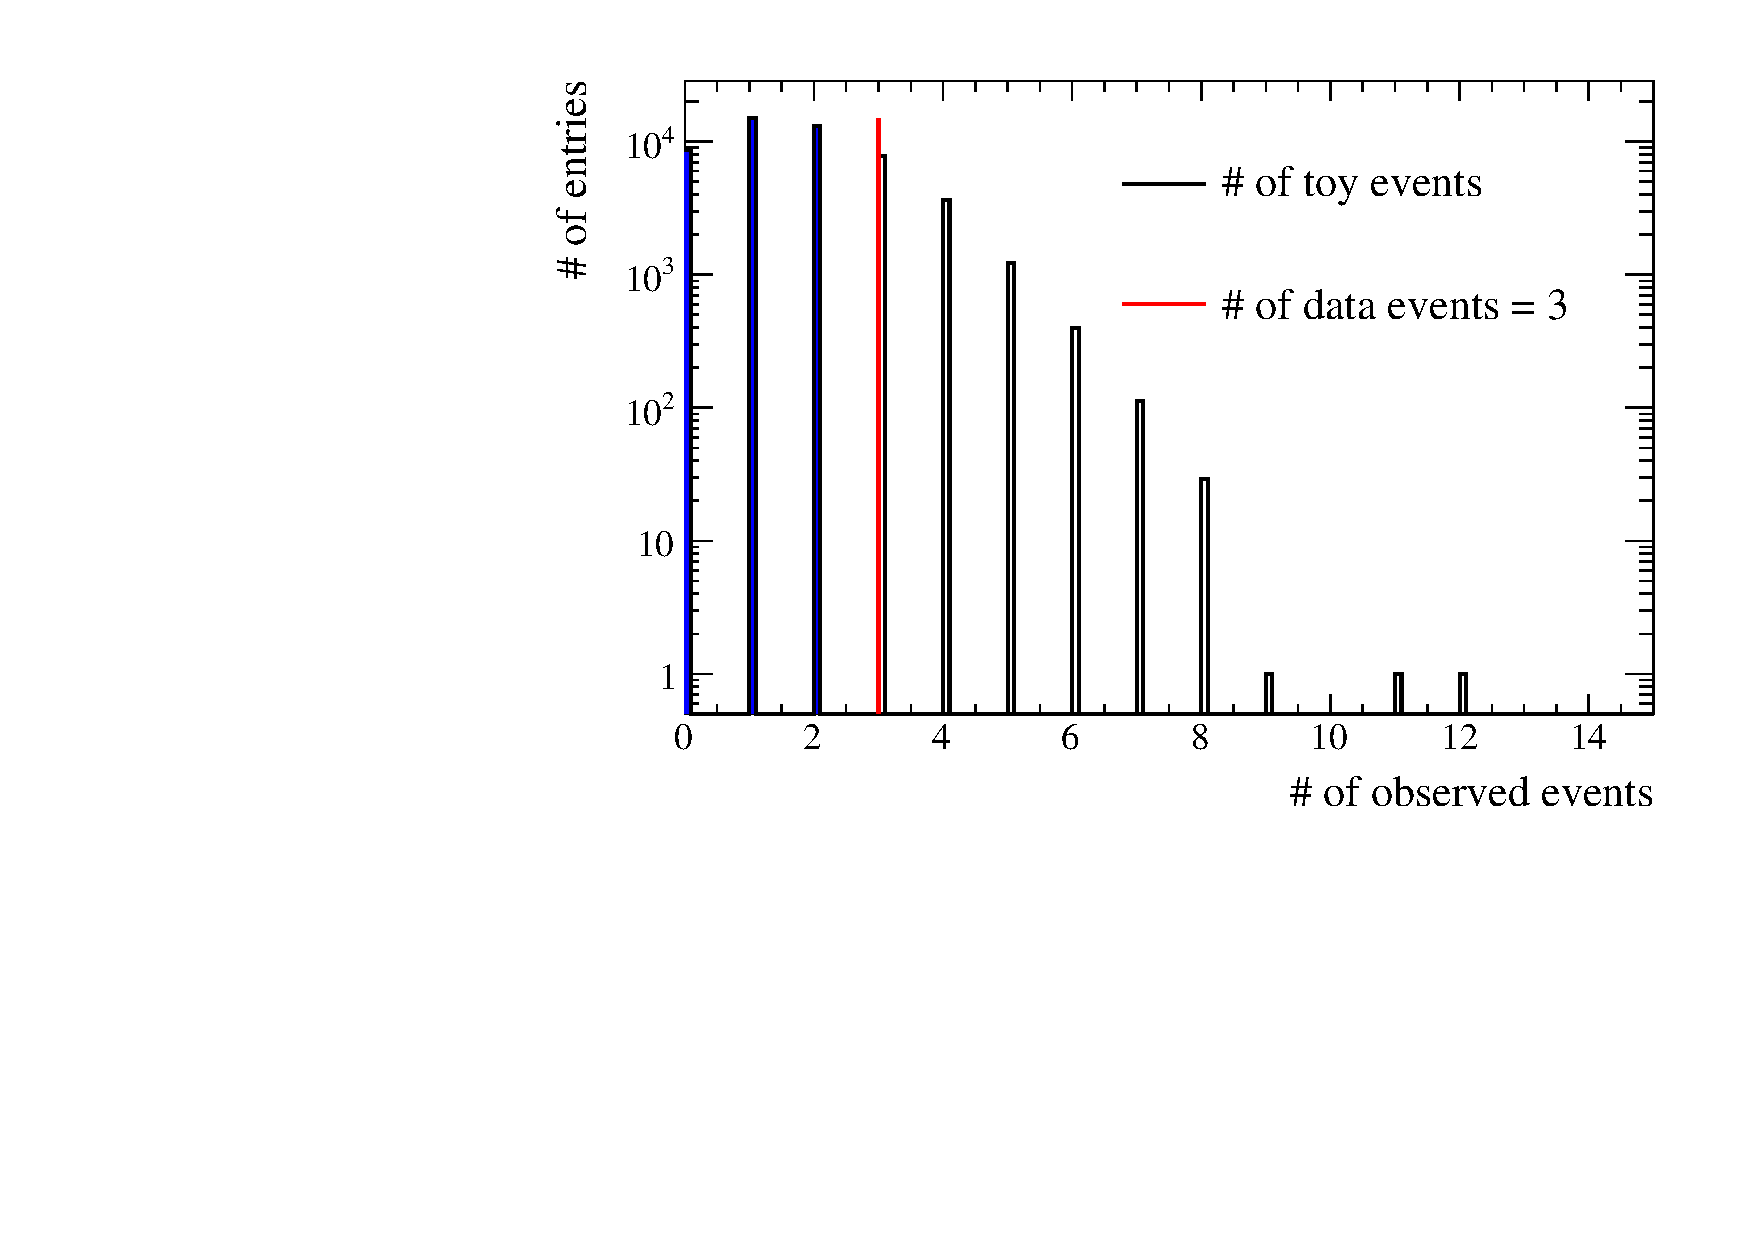
\includegraphics[width=0.9\textwidth]{./nuebar_plots/results/pvalue_rateonly_50ktoys}
%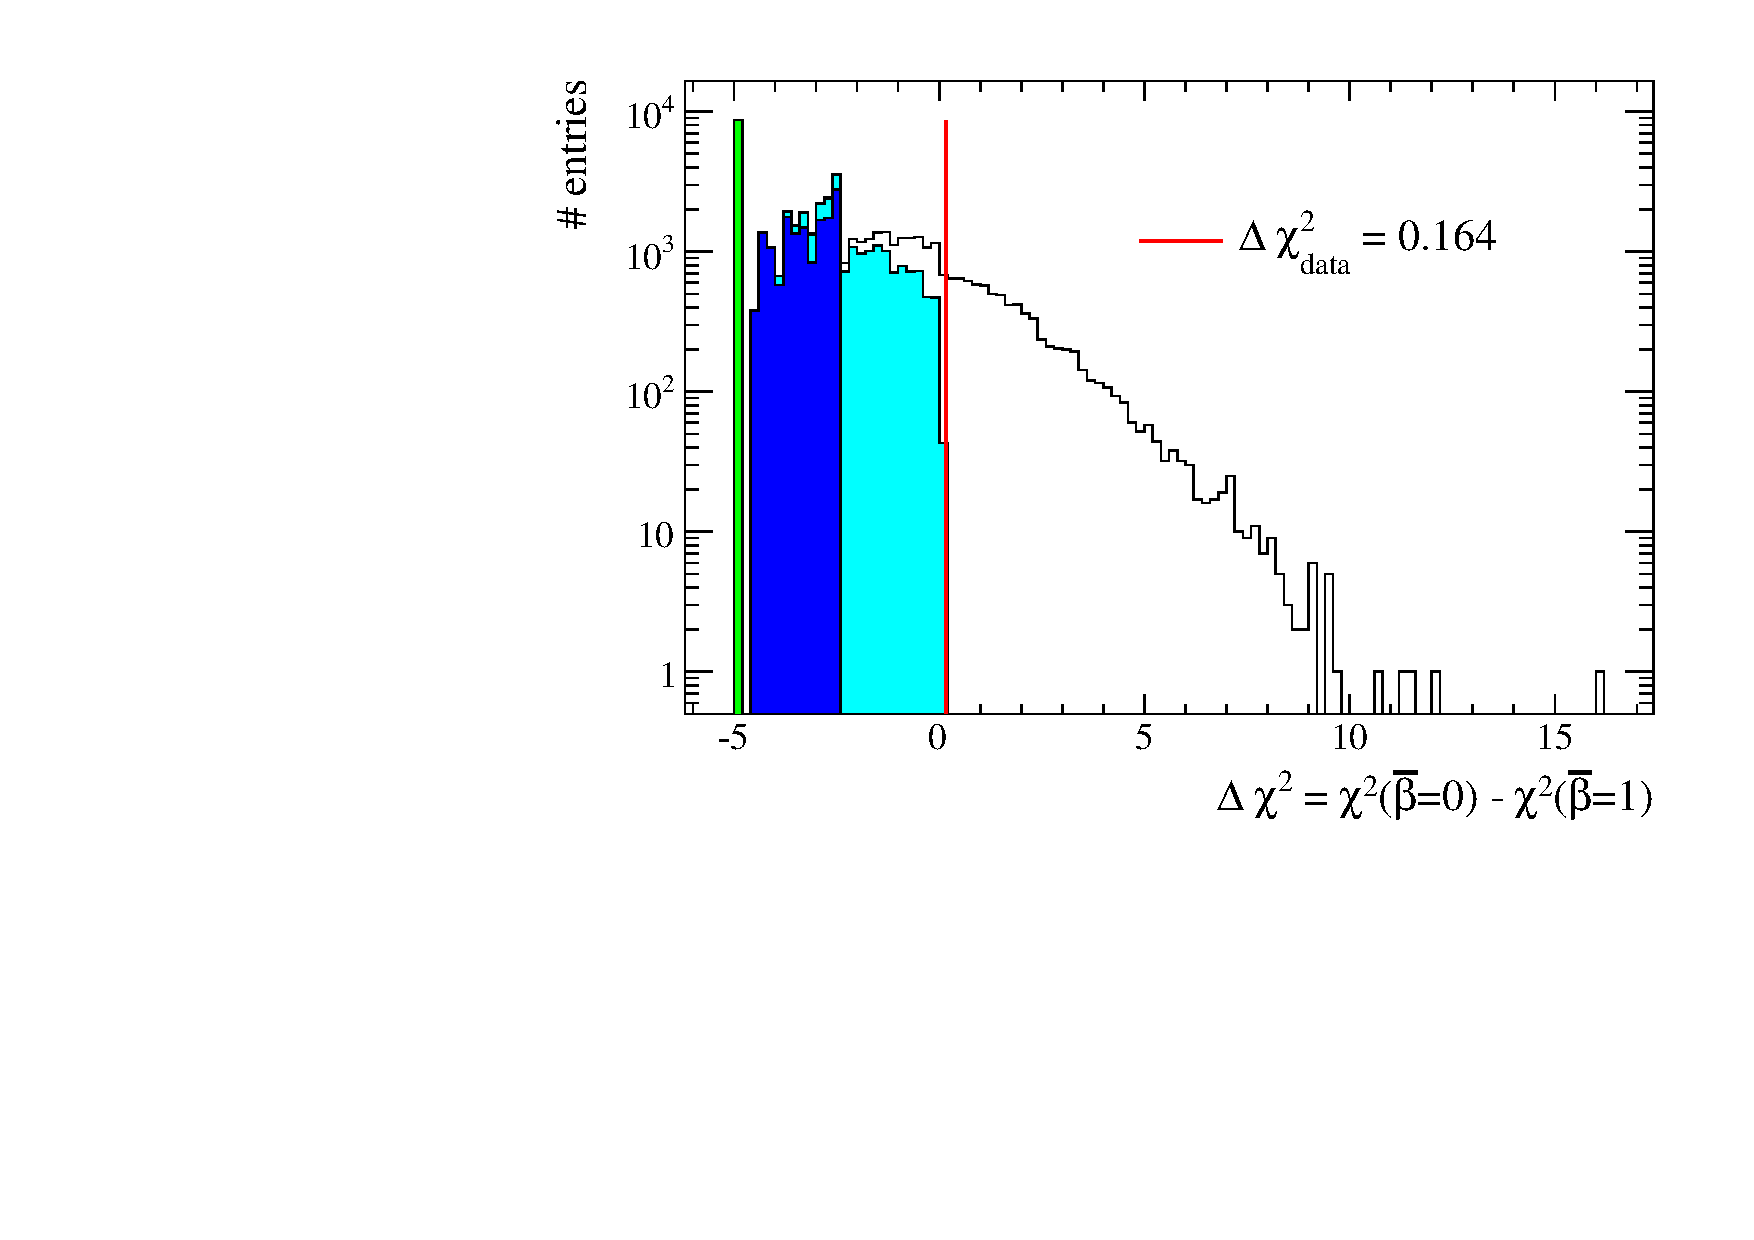
\includegraphics[width=0.9\textwidth]{./nuebar_plots/results/pvalue_rateshape_50ktoys}
\begin{subfigure}[b]{0.49\textwidth}

\includegraphics[width=0.9\textwidth]{./images/missing_plot-eps-converted-to.pdf}
\caption{Caption}
\end{subfigure}
\begin{subfigure}[b]{0.49\textwidth}

\includegraphics[width=0.9\textwidth]{./images/missing_plot-eps-converted-to.pdf}
\caption{Caption}
\end{subfigure}
\caption {
%{\huge TO UPDATE} 
The distribution of the total number of events from each of the \NumToysLarge toy experiments. 
The red line corresponds to the total number of events (left) and $\Delta \chi^2$ (right) given by the Run 5+6 dataset. 
Data correspond to Run 1-6 statistic. %\TotalPot POT.
The distribution of the test statistics are obtained by performing 50k toys. 
%\FakePotLow POT (left) and \FakePotHigh (right).
}
\label{fig:pvalue_rateonly_data}
\end{figure}


%...........................................................
%
% Table summarizing p-value for different test statistics
%
\begin{table}[htb]
\centering
\begin{tabular}{| c | c | c | c | c | c |}
\hline
Observed num. of events 		& p-value (rate-only)	 	& $\chi^2 (\beta=0)$ 		& $\chi^2 (\beta=1)$	 	& $\Delta \chi^2$ 	& p-value (rate+shape)  	\\
\hline
X				 		& XXX 		 		& XXX				& XXX				& XXX		 	& XXX			  	\\

\hline
\end{tabular}
\caption{
%{\huge TO UPDATE} 
Summary of observed number of events, $\chi^2$ for $\beta=0$ and $\beta=1$, $\Delta \chi^2$, rate-only and rate+shape p-values from the combined Run 5+6 dataset.
The quoted $\chi^2$ values were computed from \cref{eq:loglikemarg},
while $\Delta \chi^2$ from \cref{eq:deltachisq_rateshape} in \cref{sec:oscfit_method}.
using the reconstructed energy binning scheme given in \cref{sec:mc_templates:template_binning}.
The p-values are obtained performing \NumToysLarge toys with $\beta=0$ in order to get the distribution of the test statistic.
}
\label{tab:results}
\end{table}


%...........................................................

% Discussion about the p-value
%

The distribution of the expected test statistics, compared with the one obtained from the Run5-6 dataset, is shown in \cref{fig:pvalue_rateonly_data}.


%...........................................................
%
% Delta Chisq and # of events distributions with data overlapped signal and bkg
%

In \cref{fig:pvalue_rateonly_sigbkg} and \cref{fig:pvalue_rateshape_sigbkg}
the distributions of the test statistic, for rate-only and rate+shape analyses, are shown and compared with the data.
It is already clear that the current dataset is compatible with both $\beta=0$ and $\beta=1$, since the 
significance for both cases is not large enough.

\begin{figure}
\center
%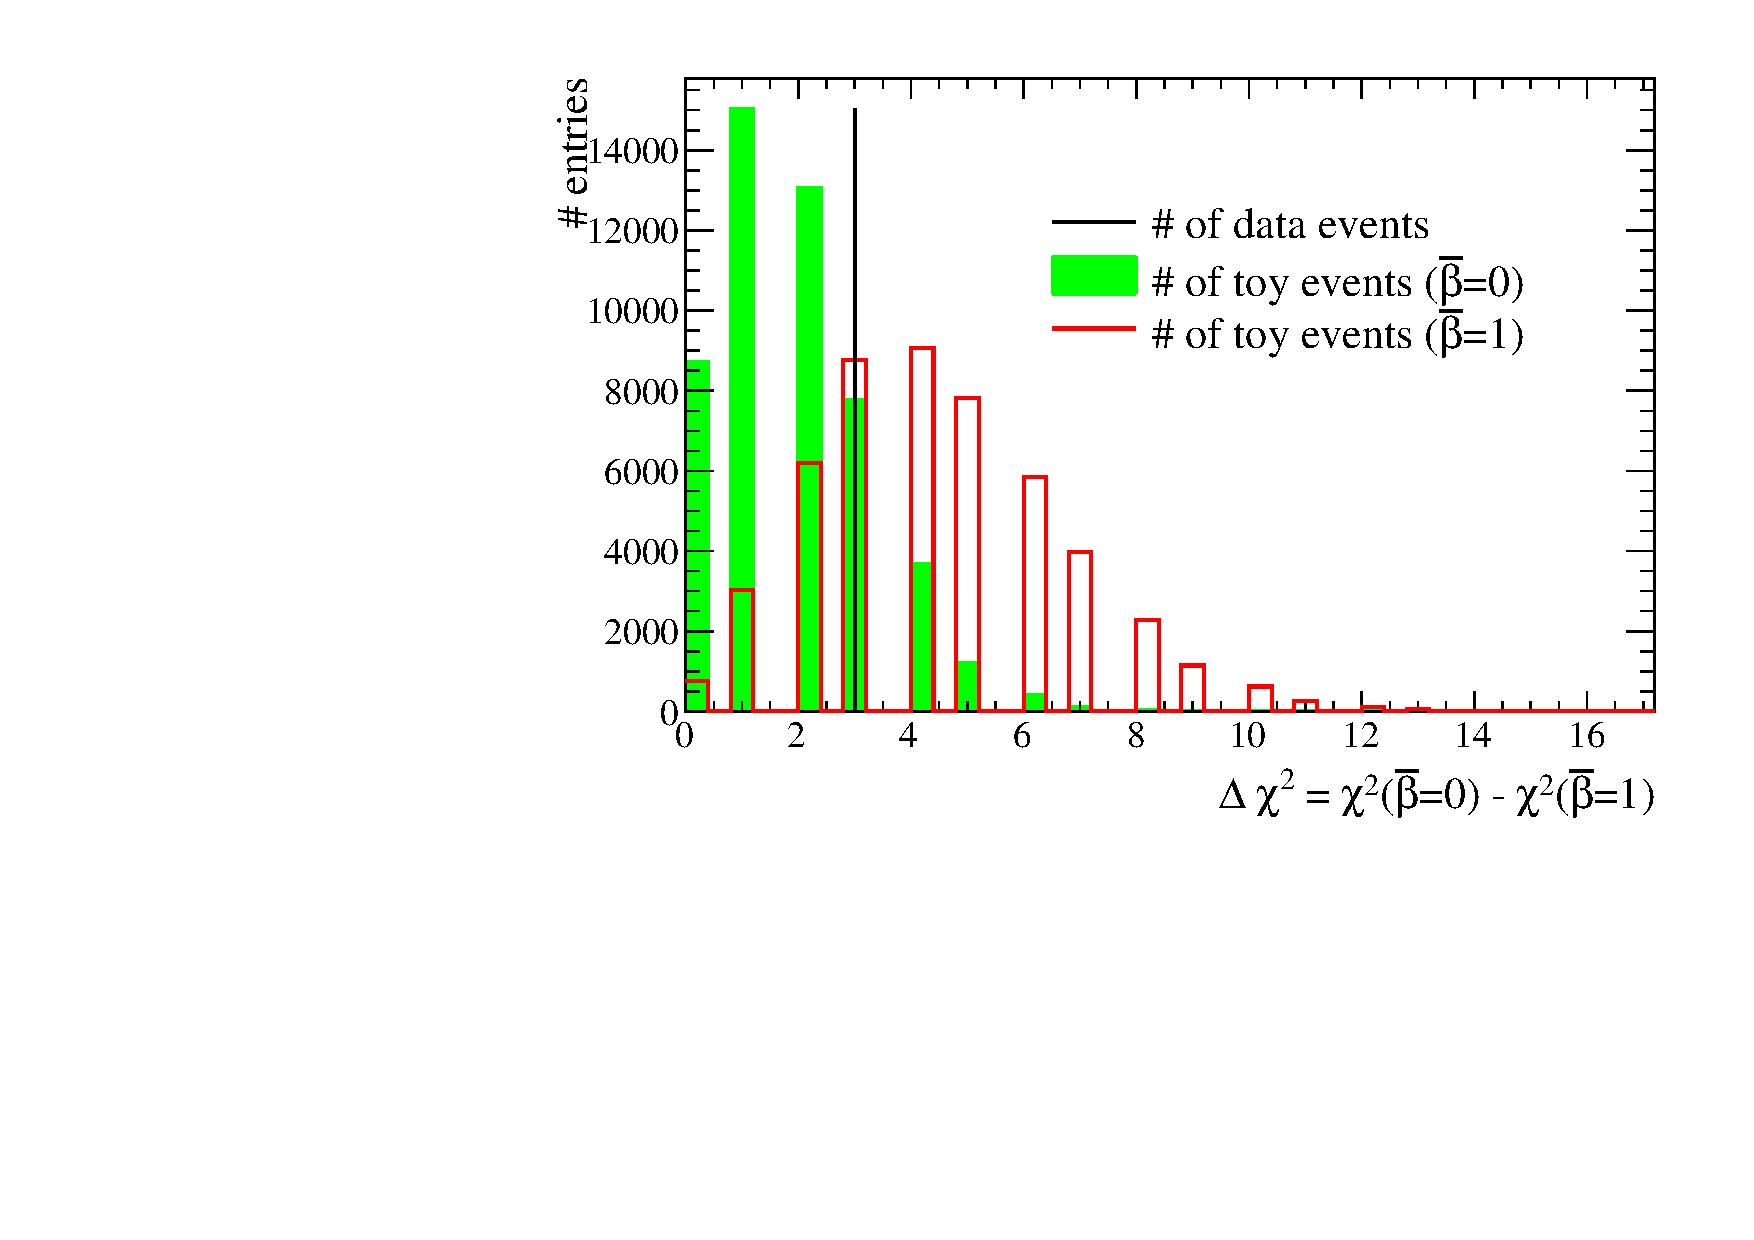
\includegraphics[width=0.9\textwidth]{./nuebar_plots/results/pvalue_rateonly_sigbkg_50ktoys.pdf}
%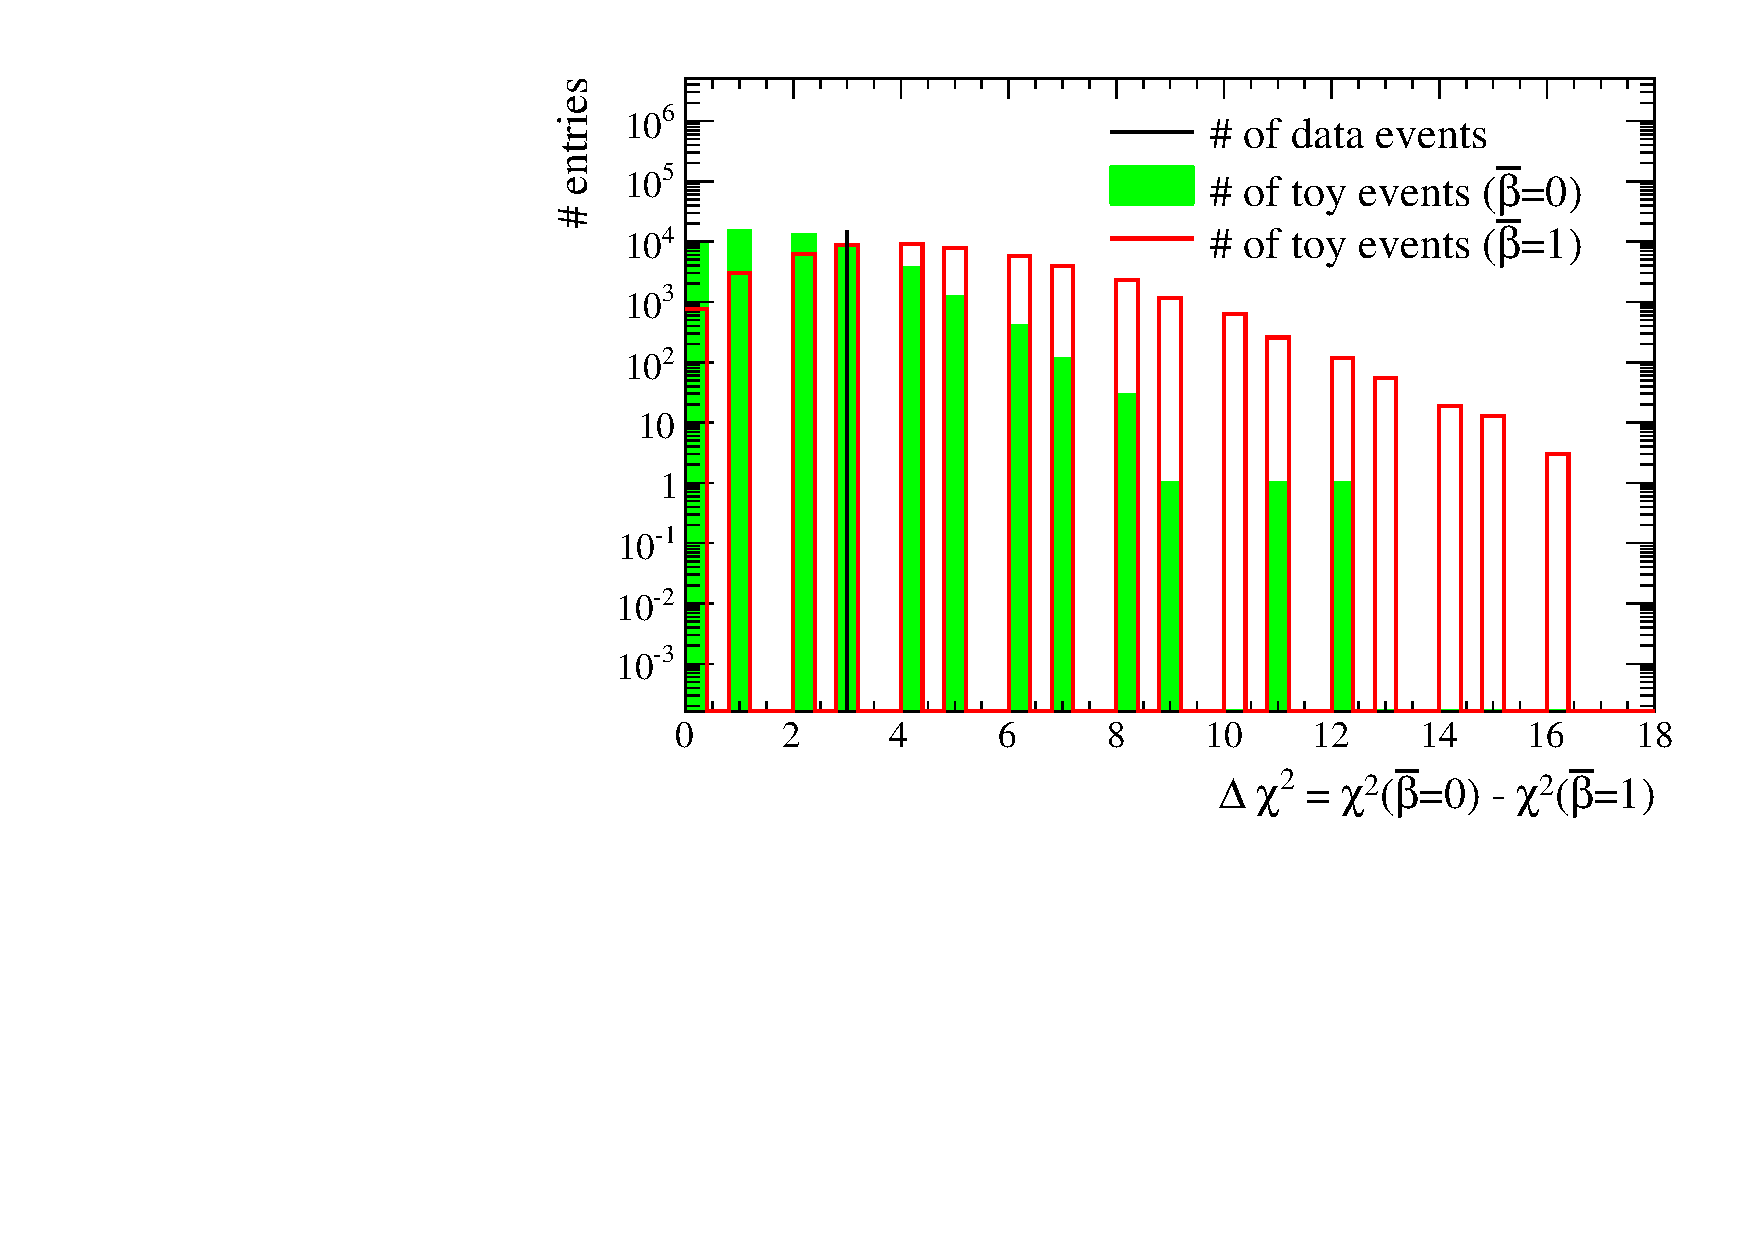
\includegraphics[width=0.9\textwidth]{./nuebar_plots/results/pvalue_rateonly_sigbkg_50ktoys_log_zoom.pdf}
\begin{subfigure}[b]{0.49\textwidth}

\includegraphics[width=0.9\textwidth]{./images/missing_plot-eps-converted-to.pdf}
\caption{Caption}
\end{subfigure}
\begin{subfigure}[b]{0.49\textwidth}

\includegraphics[width=0.9\textwidth]{./images/missing_plot-eps-converted-to.pdf}
\caption{Caption}
\end{subfigure}
\caption {
%{\huge TO UPDATE} 
The distribution of the total number of events from each of the \NumToysLarge toy experiments is
shown for both $\beta=0$ (green) and $\beta=1$ (red).
The black line corresponds to the total number of events observed in the Run 5+6 dataset. 
Data correspond to Run 1-6 statistic. %\TotalPot POT.
Both linear (left) and logarithmic (right) scales are shown.
}
\label{fig:pvalue_rateonly_sigbkg}
\end{figure}

\begin{figure}
\center
%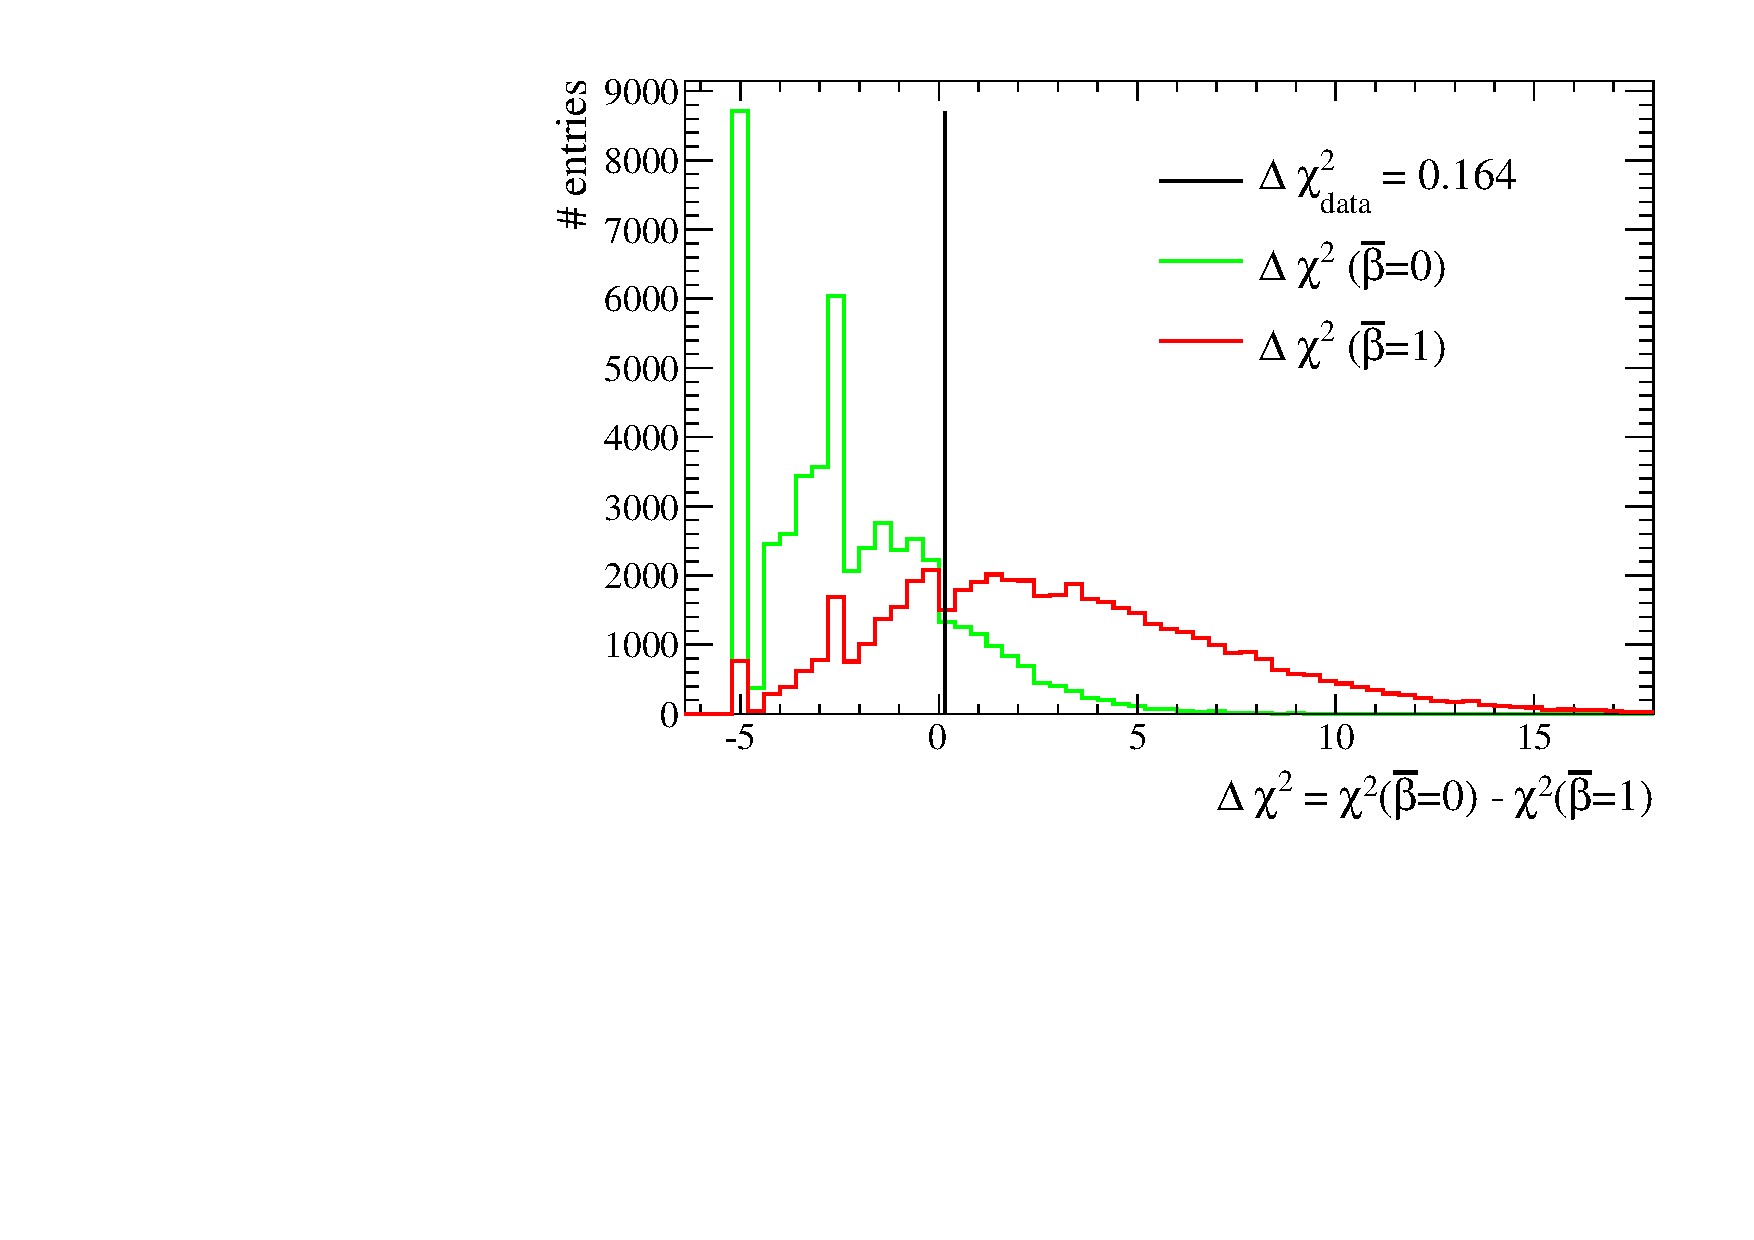
\includegraphics[width=0.9\textwidth]{./nuebar_plots/results/pvalue_rateshape_sigbkg_50ktoys.pdf}
%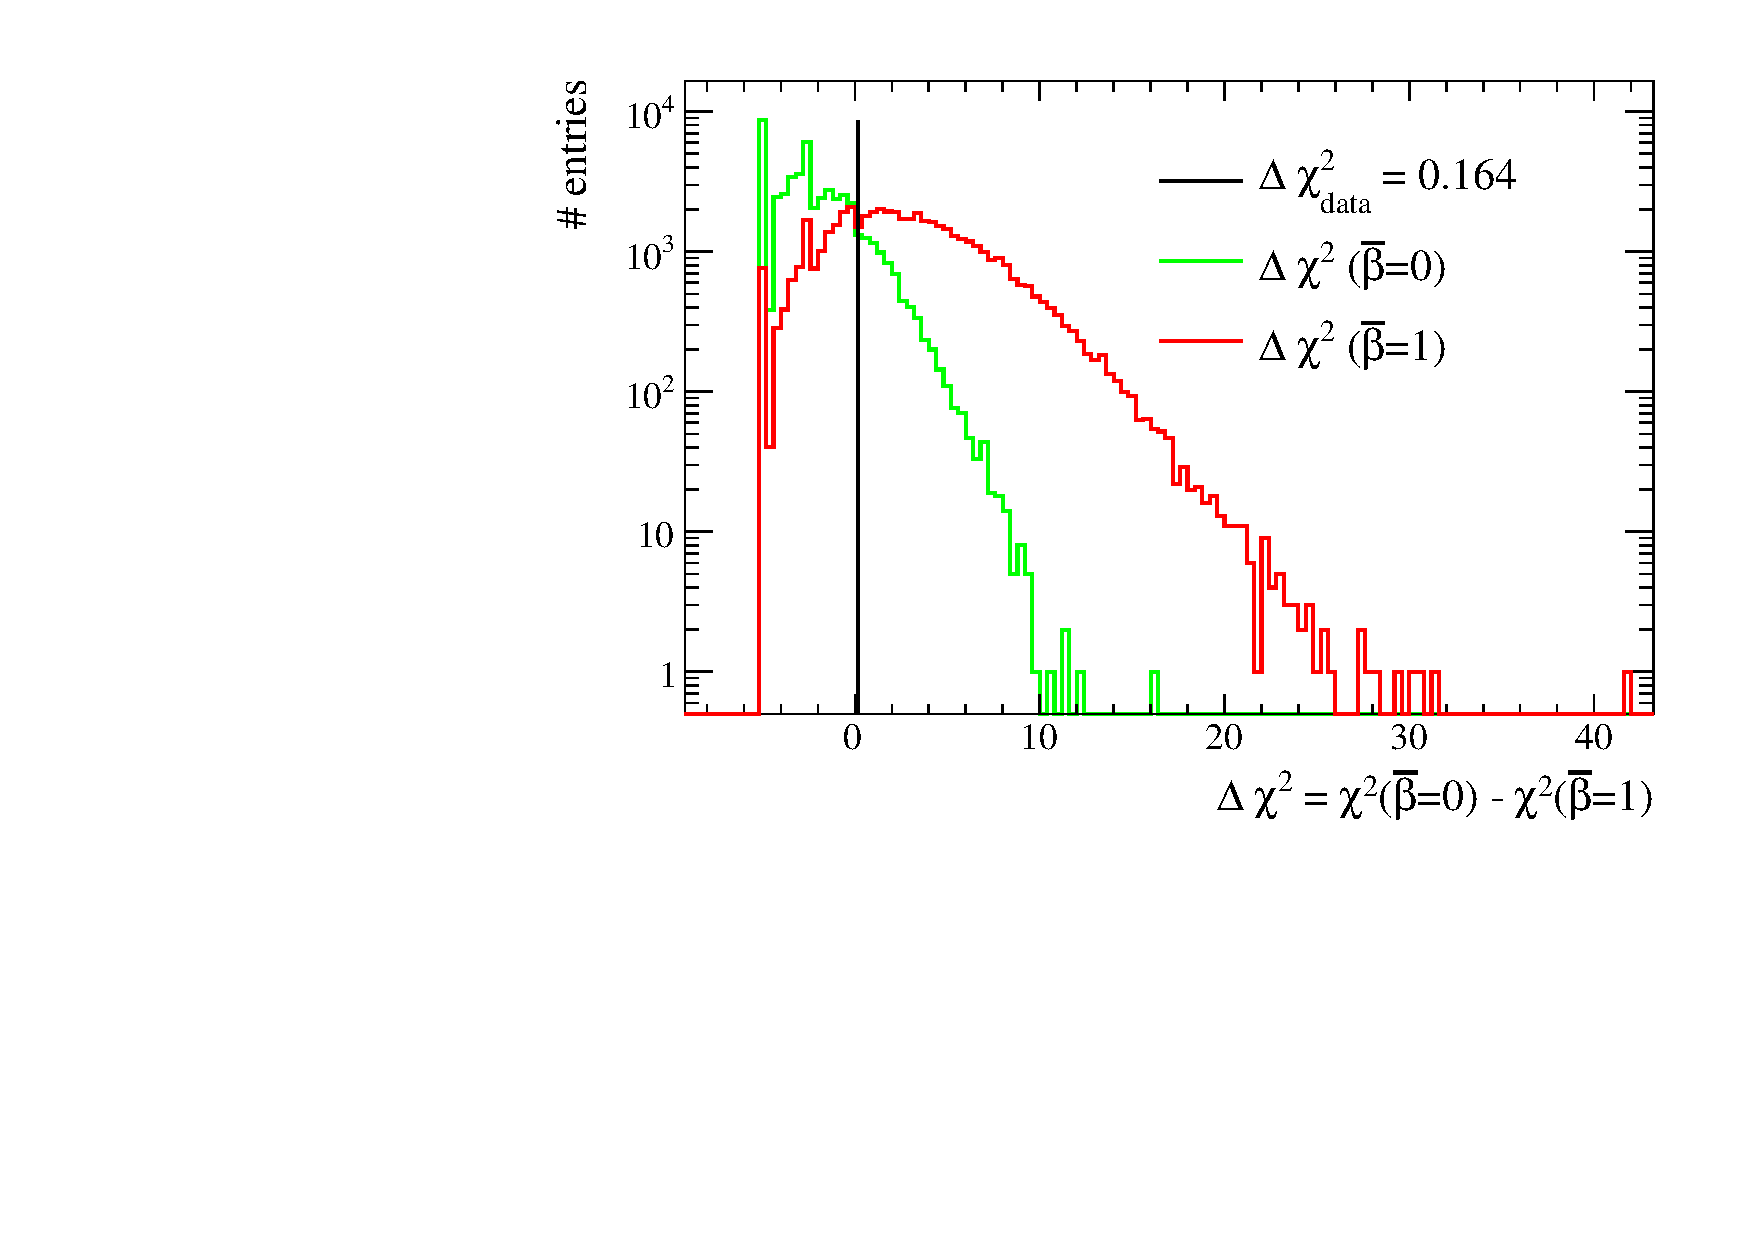
\includegraphics[width=0.9\textwidth]{./nuebar_plots/results/pvalue_rateshape_sigbkg_50ktoys_log.pdf}
\begin{subfigure}[b]{0.49\textwidth}

\includegraphics[width=0.9\textwidth]{./images/missing_plot-eps-converted-to.pdf}
\caption{Caption}
\end{subfigure}
\begin{subfigure}[b]{0.49\textwidth}

\includegraphics[width=0.9\textwidth]{./images/missing_plot-eps-converted-to.pdf}
\caption{Caption}
\end{subfigure}\caption {
%{\huge TO UPDATE} 
The distribution of the test statistic $\Delta \chi^2$ for each of the \NumToysLarge toy experiments is shown for
both $\beta=0$ (green) and $\beta=1$ (red). 
The black line corresponds to the $\Delta \chi^2$ obtained from the Run 5+6 dataset. 
Data correspond to Run 1-6 statistic. %\TotalPot POT.
Both linear (left) and logarithmic (right) scales are shown.
}
\label{fig:pvalue_rateshape_sigbkg}
\end{figure}

In order to quantify it, the 1-sided p-value given $\bar{\nu}_e$ appearance was calculated as well.
In this case, contrary to the case of null $\bar{\nu}_e$ appearance hypothesis, the 1-sided p-value
is computed on the left tail of the expected distribution of the test statistic, where the 
observed value of $\Delta \chi^2$ is placed.
As shown in \cref{tab:results_bkg} the p-value given $\bar{\nu}_e$ appearance is slightly larger than 
the background only hypothesis. The fit slightly prefers the hypothesis of $\bar{\nu}_e$ appearance,
though the significance is not large enough to claim any possible hint yet.
% of $\bar{\nu}_e$ appearance.

%...........................................................
%
% Table summarizing p-value for different test statistics
%
\begin{table}[htb]
\centering
\begin{tabular}{| c | c | c | c | c | c |}
\hline
hypothesis		 		& p-value (rate-only)	  	& p-value (rate+shape)  	\\
\hline
$\beta=0.5$			  	& 0.246 			 	& XXX			  	\\
\hline
$\beta=1$			 		& 0.089 			 	& XXX			  	\\
\hline
$\beta=1.5$				& 0.123 			 	& XXX			  	\\
\hline
$\beta=2$			 		& 0.026 			 	& XXX			  	\\
\hline
$\beta=2.5$		 		& 0.010 			 	& XXX			  	\\

\hline
\end{tabular}
\caption{
%{\huge TO UPDATE} 
Summary of 1-sided rate-only and rate+shape p-values from the combined Run 5+6 dataset.
The 1-sided p-values are obtained performing 50k toys with $\beta=0$ for background only hypothesis
and $\beta=1$ for $\bar{\nu}_e$ appearance hypothesis, in order to get the distribution of the test statistic.
In the first case the p-value given null $\bar{\nu}_e$ appearance is obtained on the right tail of the expected distribution,
while for $\beta=1$ the 1-sided p-value is obtained on the left tail of the expected distribution.
}
\label{tab:results_bkg}
\end{table}





\clearpage

\clearpage

% --------------------------------------------------------------------------------------------

\section {$\bar{\nu}_{\mu}$ disappearance analysis}
\label{sec:numubardis}

%\clearpage

\section {Analysis procedure: $\bar{\nu}_{\mu}$ dissapearance}
\label{sec:oscfit_numubardis}

%--------------------------------------------------------------------------------------------------------------------
\subsection {Fit method}
\label{sec:oscfit_method_numubardis}
The $\bar{\nu}_{\mu}$ disappearance analysis is performed in an extension of the PMNS framework with additional antineutrino oscillation parameters $\bar{\theta}_{23}$ and $|\Delta\bar{m}^{2}_{32}|$. In this framework, neutrino oscillation probabilities are calculated with the PMNS 3 flavour hypothesis whereas the antineutrino oscillation probabilities calculated with $\bar{\theta}_{23}$ and $|\Delta\bar{m}^{2}_{32}|$ along with the standard neutrino oscillation parameters $\theta_{13}$,  $\theta_{12}$, $\Delta m^{2}_{21}$, $|\Delta m^{2}_{32}|$ and mass ordering. Testing the consistency between neutrino and antineutrino disappearance probabilities in this way provides insight into the level of CPT violation in neutrino oscillations while decoupling it from the CP violation which may appear in the appearance channels. Fits are performed using the FHC 1 ring $\mu$-like and RHC 1 ring $\mu$-like samples from the full T2K Run 1-6 dataset.


The measurements of interest are as follows:
\begin{itemize}
\item 
2D $\sin^2 \theta_{23}$ Vs $|\Delta m^2_{32}|$ with reactor constraint: 
the parameters of interest are $\sin^2 \theta_{23}$ and $|\Delta m^2_{32}|$ while
all the other oscillation parameters (including $\sin^2 (\bar{\theta}_{23})$ and $\bar{|\Delta m^2_{32}|}$) are marginalised;
the gaussian prior of reactor measurements shown in Tab.~\cref{tab:osc_params_joint}, 
is used, through a penalty term as in eq.~\cref{eq:chisqmarg_with_penalty_uncorr}.

\item 
2D $\sin^2 (\bar{\theta}_{23})$ Vs $\bar{|\Delta m^2_{32}|}$ with reactor constraint: 
the parameters of interest are $\sin^2 (\bar{\theta}_{23})$ and $\bar{|\Delta m^2_{32}|}$while
all the other oscillation parameters including ($\sin^2 \theta_{23}$ and $|\Delta m^2_{32}|$) are marginalised;
the gaussian prior of reactor measurements shown in Tab.~\ref{tab:osc_params_joint}, 
is used, through a penalty term as in eq.~\ref{eq:chisqmarg_with_penalty_uncorr}.

\end{itemize}
A comparison of contours from these fits is key to determining the amount of CPT violation.

%--------------------------------------------------------------------------------------------------------------------                                                                                    

\newpage

\subsection{Sensitivity studies}
\label{sec:numubar_sensi}
All confidence level contours for sensitivity studies were were produced using the constant $\Delta \chi^2$ method described in ~\cref{sec:cl}.

In Fig.~\ref{fig:validation_sensi_numubar} the sensitivity to $\sin^2 (\bar{\theta}_{23})$ 
Vs $\bar{|\Delta m^2_{32}|}$ with reactor constraint is shown for the Asimov data set
and compared with the result obtained by the other analysis groups is shown. 

\begin{figure*}[htb]
\center

\includegraphics[width=18pc]{./images/missing_plot-eps-converted-to.pdf}

\includegraphics[width=18pc]{./images/missing_plot-eps-converted-to.pdf}
\caption {
Shown here are 68\% and 90\% constant $\Delta \chi^2$ CL contours of $\sin^2 (\bar{\theta}_{23})$ Vs $\bar{|\Delta m^2_{32}|}$
with the reactor constraint from the 3 analysis groups from a fit to the Run 1-6 Asimov dataset. Independent contours are shown 
for each hierarchy.
}
\label{fig:validation_sensi_numubar}
\end{figure*}

In Fig.~\ref{fig:validation_sensi_numubar_numu} the sensitivity to $\sin^2 (\theta_{23})$ 
Vs $|\Delta m^2_{32}|$ with reactor constraint is shown for the Asimov data set
and compared with the result obtained by the other analysis groups is shown. 

\begin{figure*}[htb]
\center

\includegraphics[width=18pc]{./images/missing_plot-eps-converted-to.pdf}

\includegraphics[width=18pc]{./images/missing_plot-eps-converted-to.pdf}
\caption {
Shown here are 68\% and 90\% constant $\Delta \chi^2$ CL  contours of $\sin^2 (\theta_{23})$ Vs $|\Delta m^2_{32}|$
with the reactor constraint from the 3 analysis groups from a fit to the Run 1-6 Asimov dataset. Contours were produced 
independently for each hierarchy hypothesis.
}
\label{fig:validation_sensi_numubar_numu}
\end{figure*}


Fig.~\ref{fig:validation_sensi_numubar_update_comparison_to_old_A,fig:validation_sensi_numubar_update_comparison_to_old_B} show a comparison of the sensitivity to $\nu$ and $\bar{\nu}$ parameters $\sin^2 (\theta_{23})$ Vs $|\Delta m^2_{32}|$ from the run 1-6 dataset to the run 1-7 dataset. There is significant improvement in the $\bar{\nu}$ parameter sensitivity in both Asimov fits with the 1-7 dataset 90\% CL inside of the run 1-6 dataset 68\% CL. Another interesting feature of the Asimov fits is that in some cases, the best fit point moves with the addition of more statistics as in Fig.~\ref{fig:validation_sensi_numubar_update_comparison_to_old_A_nubar_nh,fig:validation_sensi_numubar_update_comparison_to_old_A_nu_ih,fig:validation_sensi_numubar_update_comparison_to_old_B_nubar_nh}. Changes in the best fit point are possible when using a marginal likelihood. As seen perviously employing a marginal likelihood can lead to a best fit point away from the true parameter values because of correlations with parameters that are marginalised. In this case, the parameters marginalised are better constrained in the run 1-7 data fits than the run 1-6 and therefore have a different effect on the best fit point. 

This is however a negligible effect in the sensitivity studies as the difference in the $\Delta \chi^2$ between run 1-7 and run 1-6 Asimov fits was found to be insignificant.

\begin{figure*}[htb]
\center
    \begin{subfigure}[b]{0.49\textwidth}
        \centering
\includegraphics[width=18pc]{./numubar_plots/asimov/nh_a_nu_15_vs_16.pdf} %nubar 2015 vs 2016 nh
        \caption{$\nu$ oscillation parameter fit for normal hierarchy hypothesis}
\label{fig:validation_sensi_numubar_update_comparison_to_old_A_nu_nh}
    \end{subfigure}
    \begin{subfigure}[b]{0.49\textwidth}
        \centering
\includegraphics[width=18pc]{./numubar_plots/asimov/nh_a_nubar_15_vs_16.pdf} %nubar 2015 vs 2016 nh
        \caption{$\bar{\nu}$ oscillation parameter fit for normal hierarchy hypothesis}
\label{fig:validation_sensi_numubar_update_comparison_to_old_A_nubar_nh}
    \end{subfigure}
    \begin{subfigure}[b]{0.49\textwidth}
        \centering
\includegraphics[width=18pc]{./numubar_plots/asimov/ih_a_nu_15_vs_16.pdf} %nubar 2015 vs 2016 nh
        \caption{$\nu$ oscillation parameter fit for inverted hierarchy hypothesis}
\label{fig:validation_sensi_numubar_update_comparison_to_old_A_nu_ih}
    \end{subfigure}
    \begin{subfigure}[b]{0.49\textwidth}
        \centering
\includegraphics[width=18pc]{./numubar_plots/asimov/ih_a_nubar_15_vs_16.pdf} %nubar 2015 vs 2016 nh
        \caption{$\bar{\nu}$ oscillation parameter fit for inverted hierarchy hypothesis}
\label{fig:validation_sensi_numubar_update_comparison_to_old_A_nubar_ih}
    \end{subfigure}


\caption {
Shown here are 68\% and 90\% constant $\Delta \chi^2$ CL contours of fits to $\nu$ and $\bar{\nu}$
 parameters $\sin^2 (\theta_{23})$ Vs $|\Delta m^2_{32}|$ for both the Asimov run 1-6
 and Asimov 1-7 datasets for parameter set A in tab.~\ref{tab:osc_params_joint_asimov} .
 Contours were produced independently for each hierarchy hypothesis.
 }
\label{fig:validation_sensi_numubar_update_comparison_to_old_A}
\end{figure*}

\begin{figure*}[htb]
\center
    \begin{subfigure}[b]{0.49\textwidth}
        \centering
\includegraphics[width=18pc]{./numubar_plots/asimov/nh_b_nu_15_vs_16.pdf} %nubar 2015 vs 2016 nh
        \caption{$\nu$ oscillation parameter fit for normal hierarchy hypothesis}
\label{fig:validation_sensi_numubar_update_comparison_to_old_B_nu_nh}
    \end{subfigure}
    \begin{subfigure}[b]{0.49\textwidth}
        \centering
\includegraphics[width=18pc]{./numubar_plots/asimov/nh_b_nubar_15_vs_16.pdf} %nubar 2015 vs 2016 nh
        \caption{$\bar{\nu}$ oscillation parameter fit for normal hierarchy hypothesis}
\label{fig:validation_sensi_numubar_update_comparison_to_old_B_nubar_nh}
    \end{subfigure}
    \begin{subfigure}[b]{0.49\textwidth}
        \centering
\includegraphics[width=18pc]{./numubar_plots/asimov/ih_b_nu_15_vs_16.pdf} %nubar 2015 vs 2016 nh
        \caption{$\nu$ oscillation parameter fit for inverted hierarchy hypothesis}
\label{fig:validation_sensi_numubar_update_comparison_to_old_B_nu_ih}
    \end{subfigure}
    \begin{subfigure}[b]{0.49\textwidth}
        \centering
\includegraphics[width=18pc]{./numubar_plots/asimov/ih_b_nubar_15_vs_16.pdf} %nubar 2015 vs 2016 nh
        \caption{$\bar{\nu}$ oscillation parameter fit for inverted hierarchy hypothesis}
\label{fig:validation_sensi_numubar_update_comparison_to_old_B_nubar_ih}
    \end{subfigure}
\caption {
Shown here are 68\% and 90\% constant $\Delta \chi^2$ CL contours of fits to $\nu$ and $\bar{\nu}$
 parameters $\sin^2 (\theta_{23})$ Vs $|\Delta m^2_{32}|$ for both the Asimov run 1-6
 and Asimov 1-7 datasets for parameter set B in tab.~\ref{tab:osc_params_joint_asimov} .
 Contours were produced independently for each hierarchy hypothesis.
 }
\label{fig:validation_sensi_numubar_update_comparison_to_old_B}
\end{figure*}


\begin{figure*}[htb]
\center
    \begin{subfigure}[b]{0.49\textwidth}
        \centering
\includegraphics[width=18pc]{./numubar_plots/asimov/nu_vs_nubar_2016.pdf}
        \caption{Normal hierarchy}
\label{fig:validation_sensi_nu_vs_nubar_comparison_A_nh}
    \end{subfigure}
    \begin{subfigure}[b]{0.49\textwidth}
        \centering
\includegraphics[width=18pc]{./numubar_plots/asimov/nu_vs_nubar_2016_ih.pdf} 
        \caption{Inverted hierarchy}
\label{fig:validation_sensi_nu_vs_nubar_comparison_A_ih}
    \end{subfigure}


\caption {
Shown here are a comparison of the 68\% and 90\% constant $\Delta \chi^2$ CL contours
 of fits to $\nu$ and $\bar{\nu}$ parameters $\sin^2 (\theta_{23})$ Vs $|\Delta m^2_{32}|$
 for the Asimov 1-7 dataset for parameter set A in tab.~\ref{tab:osc_params_joint_asimov} .
 Contours were produced independently for each hierarchy hypothesis.
 }
\label{fig:validation_sensi_nu_vs_nubar_comparison_A}
\end{figure*}

\begin{figure*}[htb]
\center
    \begin{subfigure}[b]{0.49\textwidth}
        \centering
\includegraphics[width=18pc]{./numubar_plots/asimov/nu_vs_nubar_2016_B.pdf} 
        \caption{Normal hierarchy}
        \label{fig:validation_sensi_nu_vs_nubar_comparison_B_nh}
    \end{subfigure}
    \begin{subfigure}[b]{0.49\textwidth}
        \centering
\includegraphics[width=18pc]{./numubar_plots/asimov/nu_vs_nubar_2016_B_ih.pdf} 
        \caption{Inverted hierarchy}
        \label{fig:validation_sensi_nu_vs_nubar_comparison_B_nh_ih}
    \end{subfigure}

\caption {
Shown here are a comparison of the 68\% and 90\% constant $\Delta \chi^2$ CL contours
 of fits to $\nu$ and $\bar{\nu}$ parameters $\sin^2 (\theta_{23})$ Vs $|\Delta m^2_{32}|$
 for the Asimov 1-7 dataset for parameter set B in tab.~\ref{tab:osc_params_joint_asimov} .
 Contours were produced independently for each hierarchy hypothesis.
 }
\label{fig:validation_sensi_nu_vs_nubar_comparison_B}
\end{figure*}


%--------------------------------------------------------------------------------------------------------------------
\subsection {Results of the $\bar{\nu}_{\mu}$ disappearance analysis}
\label{sec:oscfit_method_numubardis}






\clearpage


% Summary and acknowledgements
\clearpage

% --------------------------------------------------------------------------------------------

\section {Summary}
\label{sec:summary}

In this technical note,
we have presented the results of the 3-flavour $\bar{\nu}/\nu$ joint analysis
performed by the {\em VALOR} group,
on the combined Run 1-6 data set,
for an exposure of \TotalPotNu{} POT in neutrino mode
and \TotalPotNuBar{} POT in antineutrino mode. 
The goal of the analysis is to search for CP violation in the leptonic
and put limits on $\delta_{CP}$ as well as 
measure all the other oscillation parameters to which T2K is sensitive:
$\sin^2 \theta_{13}$, $\sin^2 \theta_{23}$, $\Delta m^2_{32}$ ($\Delta m^2_{13}$)
and partially mass hierarchy, to which T2K has little sensitivity.

This analysis predicts 
\NskOscExpectationNumu{} $\pm$ \NskOscExpectationNumuError{} (syst) for neutrino $\mu$-like,
\NskOscExpectationNumuBar{} $\pm$ \NskOscExpectationNumuBarError{} (syst) for antineutrino $\mu$-like,
\NskOscExpectationNue{} $\pm$ \NskOscExpectationNueError{} (syst) for neutrino $e$-like,
and
\NskOscExpectationNueBar{} $\pm$ \NskOscExpectationNueBarError{} (syst) for antineutrino $e$-like
single ring events in Super K
and observes respectively 
\NskObservedNumu{} for neutrino $\mu$-like,
\NskObservedNumuBar{}  for antineutrino $\mu$-like,
\NskObservedNue{}  for neutrino $e$-like,
\NskObservedNueBar{}  for antineutrino $e$-like.

The $\bar{\nu}/\nu$ analysis was performed
in a framework of 3-flavour oscillations including matter effects in constant-density matter.
The observed reconstructed energy spectrum of single $\mu$-like ring events
and reconstructed energy versus lepton angle of single $e$-like ring events
was used to compute the confidence intervals.
All \NSyst{} systematic parameters as well as the oscillation parameters
which were not parameters of interest considered in this analysis were marginalised.

From the fit of the Run 1-6 data we can see that the favored value of $\delta_{CP}$ is -1.854, close to $-\pi/2$.
When the constant $\Delta \chi^2$ method is used $\delta_{CP}=0$ is excluded at 90\% CL
and a large portion between $0$ and $+\pi$ is excluded at $2\sigma$ if normal hierarchy is considered.
In case of inverted hierarchy a not negligible range of $\delta_{CP}$ around $+\pi/2$ is excluded with 
a significance of $3\sigma$.

From the contour of $\sin^2 \theta_{13}$ Vs $\delta_{CP}$ without the reactor constraint 
it is clear that the T2K data are in agreement with the reactor measurements within $1\sigma$ 
if $\delta_{CP} \sim -\pi/2$.

It has also been shown that the result is dominated by the excess of event in the neutrino mode
$e$-like sample, though the antineutrino mode $e$-like also prefers values of $\delta_{CP}$ 
close to $-\pi/2$, though the significance is not high.


%\vspace{3mm}
%{\huge{
%TODO: ADD COMMENTS ABOUT BEST-FIT OSCILLATION PARAMETERS
%AND 1SIGMA RANGES
%}}
%\vspace{3mm}

%\vspace{3mm}
%{\huge{
%TODO: ADD COMMENTS ABOUT GOODNESS OF FIT
%}}
%\vspace{3mm}

%\vspace{3mm}
%{\huge{
%TODO: ADD COMMENTS ABOUT 1D CONTOURS
%}}
%\vspace{3mm}
%
%\vspace{3mm}
%{\huge{
%TODO: ADD COMMENTS ABOUT 2D CONTOURS
%}}
%\vspace{3mm}





\clearpage


% References
%
% References
%

\begin{thebibliography}{9}

%
% Our previous analyses
%
\bibitem{OurRun1DisappAnalysis}
   C.Andreopoulos, T.Dealtry, J.Dobson, N.Grant, M.Haigh, J.Ilic, G.Pearce and A.Weber,
   T2K 3.23$\times10^{19}$-POT Muon-Neutrino Disappearance Analysis,
   T2K-TN-036(v4),\\
   http://www.t2k.org/docs/technotes/036
\bibitem{OurRun12DisappAnalysis}
   C.Andreopoulos, T.Dealtry, J.Dobson, N.Grant, M.Haigh, J.Ilic, G.Pearce and A.Weber,
   T2K 1.431$\times10^{20}$-POT Muon-Neutrino Disappearance Analysis
   T2K-TN-064(v3),\\
   http://www.t2k.org/docs/technotes/064
\bibitem{OurRun12DisappAnalysis3Flavour}
   C.Andreopoulos, T.Dealtry, L.Escudero, N.Grant and A.Weber,
   T2K 1.431$\times10^{20}$-POT 3-Flavour Muon-Neutrino Disappearance Analysis
   T2K-TN-087(v1),\\
   http://www.t2k.org/docs/technotes/087
\bibitem{OurRun123DisappAnalysis3Flavour}
   C.Andreopoulos, T.Dealtry, L.Escudero, N.Grant and A.Weber,
   T2K 3.010$\times10^{20}$-POT 3-Flavour Muon-Neutrino Disappearance Analysis
   T2K-TN-141(v10),\\
   http://www.t2k.org/docs/technotes/141
\bibitem{OurRun1234aDisappAnalysis3Flavour}
   C.Andreopoulos, T.Dealtry, L.Escudero, N.Grant and A.Weber,
   T2K 6.3933$\times10^{20}$-POT 3-Flavour Muon-Neutrino Disappearance Analysis
   T2K-TN-155(v2),\\
   http://www.t2k.org/docs/technotes/155
\bibitem{OurRun1234DisappAnalysis3Flavour}
   C.Andreopoulos, T.Dealtry, L.Escudero, N.Grant and A.Weber,
   T2K 6.57$\times10^{20}$-POT 3-Flavour Muon-Neutrino Disappearance Analysis
   T2K-TN-183(v3),\\
   http://www.t2k.org/docs/technotes/183
\bibitem{OurRun123JointOscillationAnalysis}
   C.Andreopoulos et al.,
   T2K 3.010$\times10^{20}$-POT Joint 3-Flavour Oscillation Analysis
   T2K-TN-154(v3),\\
   http://www.t2k.org/docs/technotes/154
\bibitem{OurRun1234JointOscillationAnalysis}
   C.Andreopoulos et al.,
   T2K 6.57$\times10^{20}$-POT Joint 3-Flavour Oscillation Analysis
   T2K-TN-175,\\
   http://www.t2k.org/docs/technotes/175
\bibitem{OurRun56AntiNumuDisappearanceAnalysis3Flavour}
   C.Andreopoulos et al.,
   T2K 2.315$\times10^{20}$-POT 3-Flavour Muon-Antineutrino Disappearance Analysis
   T2K-TN-243,\\
   http://www.t2k.org/docs/technotes/243
\bibitem{OurRun56AntiNueBarAppearanceAnalysis3Flavour}
   C.Andreopoulos et al.,
   T2K 4.0108$\times10^{20}$-POT 3-Flavour Electron-Antineutrino Appearance Analysis
   T2K-TN-252,\\
   http://www.t2k.org/docs/technotes/252

%
% Supplementary material to this analysis
%
\bibitem{OurRun1234DisappAnalysisSupplement}
  C.Andreopoulos, T.Dealtry, L.Escudero and N.Grant,
  T2K 6.5700$\times10^{20}$-POT 3-Flavour Muon-Neutrino Disappearance Analysis:
  Supplementary material on the effect of systematics,
  T2K-TN-183 supplement,\\
  http://www.t2k.org/docs/technotes/183

%
% Our previous published analyses
%
\bibitem{T2KRun12Disapp}
   T2K Collaboration (K.Abe et al.), 
   First Muon-Neutrino Disappearance Study with an Off-Axis Beam,
   Phys.Rev.D85:031103, 2012; arXiv:1201.1386
\bibitem{T2KRun123Disapp}
  T2K Collaboration (K.Abe et al.),
  Measurement of Neutrino Oscillation Parameters from Muon Neutrino Disappearance with an Off-axis Beam,
  arXiv:1308.0465 [hep-ex], 2013.
  
%
% T2K papers and drafts
%
\bibitem{T2KLongPaper}
   T2K Collaboration (K.Abe et al.),
   Measurement of neutrino oscillation in appearance and disappearance channels by the T2K experiment with 
   6.6$\times$10$^{20}$ protons on target 
   http://www.t2k.org/comm/pubboard/JournalPapers/oa2014prd/draft3

%
% p-theta TN
%
\bibitem{ptheta}
XXX

%
% Official 2012 analysis inputs and software packages
%
\bibitem{Neut:ActaP}
  Y.Hayato, A neutrino interaction simulation program library NEUT,
  Acta Phys.Polon.B40:2477-2489,2009.
\bibitem{FluxTuning}
   Beam WG, Flux tuning (11b v3.2), http://www.t2k.org/beam/NuFlux/FluxRelease/11brelease/11btuned-v3.2
\bibitem{SuperkErrors}
   M.Otani and J.Kameda,
   Super-K events and Updated systematic errors for $\nu_\mu$ disappearance analysis with T2K 1.431$\times10^{20}$ POT
   T2K-TN-065(v6),
   http://www.t2k.org/docs/technotes/065
\bibitem{NEUTnuclear}
  P. de Perio et al.,
  NEUT nuclear effects (FSI)
  T2K-TN-033(v2.0),
  http://www.t2k.org/docs/technotes/033
\bibitem{NIWGErr}
  P. de Perio et al.,
  Cross section parameters for the 2012a oscillation analysis
  T2K-TN-108(v1.3),
  http://www.t2k.org/docs/technotes/108
\bibitem{MoreNIWGErr113}
  P. de Perio et al.,
  Implementation of the NIWG cross-section parametrization,
  T2K-TN-113(v1.2) 
\bibitem{NIWGNuBarErr}
  Y.Hayato, K.McFarland, and M.Wascko (Private communication) 
% \bibitem{BANFF}
%   P. de Perio et al.,
%   Constraining the Flux and Cross Section Models with Data from the
%   ND280 Detector for the 2012a Oscillation Analysis,
%   T2K-TN-106(v8.0)
%   http://www.t2k.org/docs/technotes/106
\bibitem{SI}
  P. de Perio et al.,
  Pion Hadronic Secondary Interactions in Super-Kamiokande,
  T2K-TN-105(v1.1)
  http://www.t2k.org/docs/technotes/105
\bibitem{OldDisappSuper-K}
  Y. Ashie et al., Phys. Rev. Lett. 93, 101801 (2004);
  Y. Ashie et al., Phys. Rev. D71, 112005 (2005); 
  J. Hosaka et al., Phys. Rev. D 74, 032002 (2006).
\bibitem{FluxTuningHistograms}
  Beam group,
  http://www.t2k.org/beam/NuFlux/FluxRelease/11arelease/11atuned-v2.3.
% \bibitem{1overMAQE2}
%   M. Hartz,
%   BANFF Fit Update for the 2012 Disappearance Analyses,
%   http://www.t2k.org/asg/meeting/20121015/banffinputsdisapp/view.

%
% Official 2013 inputs
%

\bibitem{ND280Inputs}
  M. Wilking,
  Status of the 2013 ND280 $\nu_{\mu}$ analysis,\\
  http://www.t2k.org/asg/meeting/20130411/nd280numustatus/view.
\bibitem{BANFF2013}
  M. Hartz, A. Kaboth, and K. Mahn,
  Constraining the Flux and Cross Section Models with Data from the
  ND280 Detector for the 2013 Oscillation Analysis,
  T2K-TN-166(v3.0)
  http://www.t2k.org/docs/technotes/166.
\bibitem{BANFF2015}
  M. Hartz, A. Kaboth, K. Mahn, Jordan Myslik, Christine Nielsen and Mark Scott,
  Constraining the Flux and Cross Section Models with Data from the
  ND280 Detector for the 2014/2015 Oscillation Analysis,
  T2K-TN-220(v1.0)
  http://www.t2k.org/docs/technotes/220.
\bibitem{BANFF2016}
  M. Hartz, A. Kaboth, K. Mahn, Jordan Myslik, Christine Nielsen and Mark Scott,
 ND280 Flux and Cross Section Constraint (BANFF) for 2015/16,
  T2K-TN-230(v.1.0)
  http://www.t2k.org/docs/technotes/230.
\bibitem{SuperkErrors_numu}
J. Kameda,
``Updated study of the systematic error in $\nu_{\mu}$ disappearance analysis from Super-Kamiokande",
T2K-TN-159
\bibitem{SuperkErrors_nue}
J. Albert et al.,
``Study on SK $\nu_e$ candidates and systematic errors with T2K $3.23 \times 10^{19}$ POT data"
T2K-TN-157
\bibitem{SuperkEScale2013}
   J. Hignight et al.,
   Super-Kamiokande events and data quality studies for T2K Run4
   T2K-TN-148(v2r3),
   http://www.t2k.org/docs/technotes/148.

%
% Official 2015 inputs 
%

\bibitem{SuperkMC14a}
   14a data and MC info
   http://www.t2k.org/t2ksk/documentation-page/MCWeighting/MCReweighting14a

\bibitem{NCGamma}
   E. Wang, L. Alvarez-Ruso, Y. Hayato, K. Mahn, J. Nieves
   "Photon emission in neutral current interactions at the T2K experiment"
   http://arxiv.org/pdf/1507.02446v1.pdf

\bibitem{splineinfo}
   2015 SK splines
   http://www.t2k.org/asg/oagroup/inputs/201415/2015SKsplines

\bibitem{FluxTuning13a}
   Super-K 13a flux release
   http://www.t2k.org/beam/NuFlux/FluxRelease/13arelease
   
\bibitem{NIWGCCQE}
   A. Bercellie et al.
   Cross section parameters for 2014 oscillation analysis.
   T2K-TN-192 (v2.1)
   http://www.t2k.org/docs/technotes/192/ .
%
%
%


\bibitem{KDIRun1234DisappAnalysis}
  T. Wongjirad, A. Minamino and J. Kameda,
  Muon neutrino disappearance analysis with T2K 6.57 $\times$ 10$^{20}$ POT data,
  T2K-TN-164(v4),
  http://www.t2k.org/docs/technotes/164
\bibitem{2013nueptheta}
  C. Bronner et al.,
  Run1-4 p-theta electron neutrino appearance analysis,
  T2K-TN-161(v2.6),
  http://www.t2k.org/docs/technotes/161
\bibitem{2013nuenergy}
  Y. Nishimura, J. Hignight, and S. Nakayama
  $\nu_e$ appearance analysis of RUN1-4 data with neutrino energy spectrum,
  T2K-TN-162(v2.2),
  http://www.t2k.org/docs/technotes/162
  
  \bibitem{Mach3JointFitRun14} 
  A. Kaboth, R. Calland and D. Payne (Mach3)
  A Joint ND280-SK 1$\text{R}_{\mu}$-SK 1$\text{R}_e$ Fit using MCMC 
  T2K-TN-171
  http://www.t2k.org/docs/technotes/171

\bibitem{Mach3JointFitRun16} 
  K. Duffy and A. Kaboth (Mach3)
  A Joint ND280-SK 1$\text{R}_{\mu}$-SK 1$\text{R}_e$ of neutrino and antineutrino-mode data using MCMC  
  T2K-TN-269
  http://www.t2k.org/docs/technotes/269

\bibitem{Mach3ComparisonBayesFactor}
K. Duffy for the Mach3 group,
http://www.t2k.org/asg/meeting/2015-06-18/mach3\_nuebarapp

\bibitem{pthetaComparisonEreco}
H. Tanaka for the p-$\theta$ group,
http://www.t2k.org/asg/meeting/2015-06-18/nuebar\_appearance\_study

%
% External papers relevant to official inputs
%

\bibitem{NA61/SHINET2K2014}
  N Abgrall et al. Measurements of production properties of K$^{0}_{S}$ mesons and $\Lambda$ hyperons in proton-carbon interactions at 31 GeV/c
  Phys. Rev. C 89, 025205

\bibitem{NA61/SHINET2K}
  N Abgrall et al. Measurements of Cross Sections and Charged Pion Spectra in Proton-Carbon Interactions
  at 31 GeV/c. Phys.Rev., C84:034604, 2011;
  N. Abgrall et al. Measurement of production properties of positively charged kaons in proton-carbon
  interactions at 31 GeV/c. arXiv:hep-ex/1112.0150, 2011.
%
% PDG-2012 
%
\bibitem{PDG2012}
  J. Beringer et al. (Particle Data Group), Phys. Rev. D86, 010001 (2012)
%
% Talks by VALOR group members referenced in the text
%
\bibitem{Lorena}
  Lorena Escudero Sanchez for the {\em VALOR} group, 
  http://www.t2k.org/asg/oagroup/meeting/20121219/VaLOR%202012%20joint%20OA%20report/view
\bibitem{Tom1overMaQE2}
  Tom Dealtry for the {\em VALOR} group,
  http://www.t2k.org/asg/meeting/2012/20121015/valornumudisapp/view
\bibitem{slides_davide_pvalue_asg}
  Davide Sgalaberna for the {\em VALOR} group,
  http://www.t2k.org/asg/meeting/2015-05-14/view

%
% Statistics etc
%
\bibitem{Asimov} 
G.Cowan, K.Cranmer, E.Gross, O.Vitells,
"Asymptotic formulae for likelihood-based tests of new physics"
arXiv:1007.1727v2
\bibitem{StatAnalysisCowan} 
  G. Cowan (1998) Statistical data analysis, 
  Oxford University Press, ISBN 0-19-850155-2.
\bibitem{Minuit}
  F.James, M.Roos, Minuit: A System for Function Minimization and Analysis of the 
  Parameter Errors and Correlations, Comput.Phys.Commun. 10:343 (1975)
%\bibitem{NumRecipCholesky}
%  Numerical Recipes: The art of scientific computing, 
%  Cambridge University Press, 3rd Edition, ISBN 978-0-521-88068-0, pp. 100-102.
%\bibitem{RevPartPhysStat}
%  C. Amsler et al. (Particle Data Group),
%  Review of Particle Physics, Phys.Lett.B667:1,2008 
\bibitem{FeldmanCousins}
  G.J. Feldman and R.D. Cousins,
  A Unified approach to the classical statistical analysis of small signals,
  Phys.Rev.D57:3873-3889,1998; physics/9711021
\bibitem{CousinsHighland}
  R.D. Cousins and V.L.Highland, 
  Nucl.Instr. and Meth. A320:331035, 1992.
\bibitem{Kendall}
J. Stuart, A. Ord and S.Arnold,
Kendall's Advanced Theory of Statistics, Vol 2A (6th Ed.) 
(Oxford University Press, New York, 1994).
\bibitem{NickPvalue}
 N.Grant for the {\em VALOR} group,
 http://www.t2k.org/asg/meeting/2011/20111124/pvalues/view
\bibitem{KarlenPvalue}
 D.Karlen,
 p-values, distributions and low statistics,
 http://www.t2k.org/asg/oagroup/meeting/20120416/lowstat/view
 \bibitem{cl_masshierarchy}
 X. Qian, A. Tan, W. Wang, J. J. Ling, R. D. McKeown and C. Zhang,
 Statistical evaluation of experimental determinations of neutrino mass hierarchy,
 Phys.Rev.D86, 113011 (2012)
 
%
% Numu contour committe report
%
\bibitem{T2KNuMuContourCom}
  K. McFarland for the T2K $\nu_{\mu}$-disappearance contour committee 
  (C.Andreopoulos, N.Grant, J.Kameda, D.Karlen, E.Kearns, K.McFarland, M.Otani, M.Zito)
  Report to ASG conveners meeting, 17 May 2011,
  http://www.t2k.org/asg/contour/ASG-Conveners-Report/view
%
% MINOS, SK atm. "23"-sector oscillation analyses
%
\bibitem{MINOS2012}
  R.Nichol,
  Talk at Neutrino 2012
\bibitem{MINOS2013}
  P. Adamson, et al.,
  Measurement of Neutrino and Antineutrino Oscillations Using Beam and Atmospheric Data in MINOS,
  arXiv:1304.6335 [hep-ex], 2013
\bibitem{MINOS2013sinsqtheta}
  A. Radovic,
  Talk at DPF 2013
\bibitem{SKAtm2012}
  Y. Itow,
  Recent results in atmospheric neutrino oscillations in the light of large $\theta_{13}$,
  Nucl. Phys. B (Proc. Suppl.) 235 79 (2013).

\bibitem{pdg_2013}
J. Beringer et al. (Particle Data Group with 2013 update), 
Phys. Rev. D86, 010001 (2012)

\bibitem{pdg_2014}
K.A. Olive et al. (Particle Data Group 2014 with 2015 update), 
Chin. Phys. C, 38, 090001

% 
% Experiment-specific theta13, theta12, and dmsq12 refs
%
%\bibitem{Kamland}
%  S. Abe et al.,
%  Precision measurements of neutrino oscillation parameters with KamLAND
%  Phys.Rev.Lett.100:221803,2008
%\bibitem{DayaBay}
%  F.P. An et al.,
%  Observation of electron-antineutrino disappearance at Daya Bay
%  Phys.Rev.Lett.108:171803,2012
%\bibitem{Reno}
%  J.K. Ahn et al.,
%  Observation of reactor electron antineutrinos disappearance in the Reno experiment
%  Phys.Rev.Lett.108:191802,2012
%
% Global oscillation analyses
%
\bibitem{FogliLisi}
  G.L.Fogli, E.Lisi et~al.,
  Evidence of theta(13)$>$0 from global neutrino data analysis,
  Phys.Rev.D84:053007, 2011; arXiv:1106.6028 [hep-ph]
\bibitem{GonzalezGarcia}
 M.C.Gonzalez-Garcia, M.Maltoni, J.Salvado and T.Schwetz,
 Global fit to three neutrino mixing: critical look at present precision,
 arXiv:1209.3023 [hep-ph]
%\bibitem{ockham}
%  "Ockham's razor", Encyclopedia Britannica
%  http://www.britannica.com/EBchecked/topic/424706/Ockhams-razor
%
% 3-flavour oscillation probability formulas etc
%
%\bibitem{kayser2005}
%  B. Kayser (2005), Neutrino physics, hep-ph 0506165
%\bibitem{giunti}
%  C Giunti and C.W. Kim (2007) Fundamentals of neutrino physics and astrophysics, Oxford Uninversity Press
%\bibitem{pdgreview}
%  K. Nakamura and S.T. Petcov (2010) Neutrino mass, mixing and oscillations,
%  http://pdg.lbl.gov/2010/reviews/rpp2010-rev-neutrino-mixing.pdf
%\bibitem{kopp}
%  J. Kopp (2006), Efficient numerical diagonalisation of Hermitian 3x3 matrices, arXiv:physics/0610206
%
% Other 3-flavour oscillation probability packages
%
%\bibitem{sloan}
%  T. Sloan, private communication (June-July 2011)
\bibitem{Prob3}
 Prob3++ 3-flavour oscillation probability software,
 http://www.phy.duke.edu/~raw22/public/Prob3++/
 
 %\cite{Adamson:2013whj}
\bibitem{Adamson:2013whj}
  P.~Adamson {\it et al.}  [MINOS Collaboration],
  %``Measurement of Neutrino and Antineutrino Oscillations Using Beam and Atmospheric Data in MINOS,''
  Phys.\ Rev.\ Lett.\  {\bf 110} (2013) 25,  251801
  [arXiv:1304.6335 [hep-ex]].
  %%CITATION = ARXIV:1304.6335;%%
  %94 citations counted in INSPIRE as of 14 Apr 2015

\end{thebibliography}




%Appendices
\clearpage
\begin{appendices}
%%~ \addappheadtotoc

%...........................................................
%
% Predicted number of events
%
%...........................................................

\section{Predicted number of events}
\label{app:events}

%In Tab.
%\ref{tab:nsk_nominal_no_osc_mulike_nu},~\ref{tab:nsk_nominal_osc_mulike_nu},
%\ref{tab:nsk_nominal_no_osc_mulike_nubar},~\ref{tab:nsk_nominal_osc_mulike_nubar},
%\ref{tab:nsk_nominal_no_osc_elike_nu},~\ref{tab:nsk_nominal_osc_elike_nu},
%\ref{tab:nsk_nominal_no_osc_elike_nubar} and~\ref{tab:nsk_nominal_osc_elike_nubar} 
%the predicted number of events is shown for 
%nominal MC, after applying the NA61/SHINE reweighting,
%after applying the NIWG tuning and 
%finally the BANFF tuning,
%both with oscillations consistent with ~\cref{tab:osc_params_joint}
%and without oscillations.
%
%
%\begin{table}
\begin{tabular} { | c ||c | c | c | c |  | }
\hline
                                                  & Nominal MC          & Flux-tuned MC       & BANFF prefit MC     & BANFF postfit MC     \\
                                                  &                     &                     & (flux + NIWG tune)  &                      \\ \hline  
Total                                             & 96.434              & 100.439             & 87.615              & 103.604              \\ \hline 
\hline 
$\nu_\mu$ CCQE                                    & 14.186              & 14.493              & 14.250              & 15.405               \\ \hline 
$\nu_\mu$ CC 1$\pi$                               & 4.792               & 5.019               & 5.019               & 3.666                \\ \hline 
$\nu_\mu$ CC coherent                             & 0.201               & 0.212               & 0.212               & 0.244                \\ \hline 
$\nu_\mu$ CC MEC                                  & 2.630               & 2.707               & 0.731               & 3.022                \\ \hline 
$\nu_\mu$ CC other                                & 1.198               & 1.307               & 1.307               & 1.393                \\ \hline 
$\nu_\mu$/$\nu_\tau$ NC 1$\pi^{+/-}$              & 0.495               & 0.523               & 0.523               & 0.340                \\ \hline 
$\nu_\mu$/$\nu_\tau$ NC 1$\pi^0$                  & 0.081               & 0.086               & 0.086               & 0.051                \\ \hline 
$\nu_\mu$/$\nu_\tau$ NC coherent                  & 0.001               & 0.001               & 0.001               & 0.001                \\ \hline 
$\nu_\mu$/$\nu_\tau$ NC other                     & 0.434               & 0.470               & 0.470               & 0.705                \\ \hline 
$\bar{\nu}_\mu$ CCQE                              & 53.188              & 55.834              & 50.852              & 57.962               \\ \hline 
$\bar{\nu}_\mu$ CC 1$\pi$                         & 7.506               & 7.658               & 7.658               & 6.746                \\ \hline 
$\bar{\nu}_\mu$ CC coherent                       & 2.409               & 2.515               & 2.515               & 3.082                \\ \hline 
$\bar{\nu}_\mu$ CC MEC                            & 7.382               & 7.699               & 2.079               & 9.037                \\ \hline 
$\bar{\nu}_\mu$ CC other                          & 0.914               & 0.891               & 0.891               & 1.005                \\ \hline 
$\bar{\nu}_\mu$/$\bar{\nu}_\tau$ NC 1$\pi^{+/-}$  & 0.571               & 0.581               & 0.581               & 0.381                \\ \hline 
$\bar{\nu}_\mu$/$\bar{\nu}_\tau$ NC 1$\pi^0$      & 0.081               & 0.082               & 0.082               & 0.048                \\ \hline 
$\bar{\nu}_\mu$/$\bar{\nu}_\tau$ NC coherent      & 0.006               & 0.006               & 0.006               & 0.007                \\ \hline 
$\bar{\nu}_\mu$/$\bar{\nu}_\tau$ NC other         & 0.265               & 0.260               & 0.260               & 0.410                \\ \hline 
$\nu_e$ CCQE                                      & 0.003               & 0.004               & 0.003               & 0.004                \\ \hline 
$\nu_e$ CC 1$\pi$                                 & 0.003               & 0.003               & 0.003               & 0.003                \\ \hline 
$\nu_e$ CC coherent                               & 0.000               & 0.000               & 0.000               & 0.000                \\ \hline 
$\nu_e$ CC MEC                                    & 0.001               & 0.001               & 0.000               & 0.001                \\ \hline 
$\nu_e$ CC other                                  & 0.001               & 0.001               & 0.001               & 0.001                \\ \hline 
$\nu_e$ NC 1$\pi^{+/-}$                           & 0.021               & 0.021               & 0.021               & 0.014                \\ \hline 
$\nu_e$ NC 1$\pi^0$                               & 0.003               & 0.004               & 0.004               & 0.002                \\ \hline 
$\nu_e$ NC coherent                               & 0.000               & 0.000               & 0.000               & 0.000                \\ \hline 
$\nu_e$ NC other                                  & 0.022               & 0.022               & 0.022               & 0.035                \\ \hline 
Osc. $\nu_e$ CCQE                                 & 0.000               & 0.000               & 0.000               & 0.000                \\ \hline 
Osc. $\nu_e$ CC 1$\pi$                            & 0.000               & 0.000               & 0.000               & 0.000                \\ \hline 
Osc. $\nu_e$ CC coherent                          & 0.000               & 0.000               & 0.000               & 0.000                \\ \hline 
Osc. $\nu_e$ CC MEC                               & 0.000               & 0.000               & 0.000               & 0.000                \\ \hline 
Osc. $\nu_e$ CC other                             & 0.000               & 0.000               & 0.000               & 0.000                \\ \hline 
$\bar{\nu}_e$ CCQE                                & 0.005               & 0.005               & 0.004               & 0.005                \\ \hline 
$\bar{\nu}_e$ CC 1$\pi$                           & 0.002               & 0.002               & 0.002               & 0.002                \\ \hline 
$\bar{\nu}_e$ CC coherent                         & 0.000               & 0.000               & 0.000               & 0.001                \\ \hline 
$\bar{\nu}_e$ CC MEC                              & 0.001               & 0.001               & 0.000               & 0.001                \\ \hline 
$\bar{\nu}_e$ CC other                            & 0.000               & 0.000               & 0.000               & 0.000                \\ \hline 
$\bar{\nu}_e$ NC 1$\pi^{+/-}$                     & 0.016               & 0.016               & 0.016               & 0.010                \\ \hline 
$\bar{\nu}_e$ NC 1$\pi^0$                         & 0.002               & 0.002               & 0.002               & 0.001                \\ \hline 
$\bar{\nu}_e$ NC coherent                         & 0.000               & 0.000               & 0.000               & 0.000                \\ \hline 
$\bar{\nu}_e$ NC other                            & 0.011               & 0.011               & 0.011               & 0.017                \\ \hline 
Osc. $\bar{\nu}_e$ CCQE                           & 0.000               & 0.000               & 0.000               & 0.000                \\ \hline 
Osc. $\bar{\nu}_e$ CC 1$\pi$                      & 0.000               & 0.000               & 0.000               & 0.000                \\ \hline 
Osc. $\bar{\nu}_e$ CC coherent                    & 0.000               & 0.000               & 0.000               & 0.000                \\ \hline 
Osc. $\bar{\nu}_e$ CC MEC                         & 0.000               & 0.000               & 0.000               & 0.000                \\ \hline 
Osc. $\bar{\nu}_e$ CC other                       & 0.000               & 0.000               & 0.000               & 0.000                \\ \hline 

\end{tabular}
\caption{
  Calculated predicted numbers of 1-ring $\mu$-like events without oscillations using the nominal MC templates, the
  NA61-tuned MC templates, the NIWG-tuned MC templates and the BANFF-tuned MC templates.
  The BANFF prefit column is the NA61 tuned data, with the CCQE samples reweighted according to the NIWG's external data fits~\cite{NIWGCCQE}.
  The total numbers of events and the numbers of events from each mode considered in this analysis are shown.
  These numbers were calculated for an exposure of \TotalPot POT.
}
\label{tab:nsk_nominal_no_osc}
\end{table}

%________________________________________________________________________________________________________________________________________________________________________________
\begin{table}
\begin{tabular} { | c ||c | c | c | c |  | }
\hline
                                                  & $N_{SK}$            & $N_{SK}$            & $N_{SK}$            & $N_{SK}$             \\ 
                                                  & Nominal MC          & Flux-tuned MC       & BANFF prefit MC     & BANFF postfit MC     \\
                                                  &                     &                     & (flux + NIWG tune)  &                      \\ \hline 
Total                                             & 33.161              & 34.240              & 30.715              & 34.584               \\ \hline  
\hline 
$\nu_\mu$ CCQE                                    & 6.269               & 6.525               & 6.447               & 6.871                \\ \hline 
$\nu_\mu$ CC 1$\pi$                               & 3.155               & 3.349               & 3.349               & 2.415                \\ \hline 
$\nu_\mu$ CC coherent                             & 0.136               & 0.146               & 0.146               & 0.167                \\ \hline 
$\nu_\mu$ CC MEC                                  & 1.365               & 1.428               & 0.386               & 1.578                \\ \hline 
$\nu_\mu$ CC other                                & 1.049               & 1.150               & 1.150               & 1.223                \\ \hline 
$\nu_\mu$/$\nu_\tau$ NC 1$\pi^{+/-}$              & 0.495               & 0.523               & 0.523               & 0.340                \\ \hline 
$\nu_\mu$/$\nu_\tau$ NC 1$\pi^0$                  & 0.081               & 0.086               & 0.086               & 0.051                \\ \hline 
$\nu_\mu$/$\nu_\tau$ NC coherent                  & 0.001               & 0.001               & 0.001               & 0.001                \\ \hline 
$\nu_\mu$/$\nu_\tau$ NC other                     & 0.434               & 0.470               & 0.470               & 0.705                \\ \hline 
$\bar{\nu}_\mu$ CCQE                              & 12.222              & 12.584              & 11.656              & 13.278               \\ \hline 
$\bar{\nu}_\mu$ CC 1$\pi$                         & 3.556               & 3.552               & 3.552               & 3.048                \\ \hline 
$\bar{\nu}_\mu$ CC coherent                       & 0.565               & 0.574               & 0.574               & 0.697                \\ \hline 
$\bar{\nu}_\mu$ CC MEC                            & 1.978               & 2.015               & 0.544               & 2.350                \\ \hline 
$\bar{\nu}_\mu$ CC other                          & 0.805               & 0.782               & 0.782               & 0.881                \\ \hline 
$\bar{\nu}_\mu$/$\bar{\nu}_\tau$ NC 1$\pi^{+/-}$  & 0.571               & 0.581               & 0.581               & 0.381                \\ \hline 
$\bar{\nu}_\mu$/$\bar{\nu}_\tau$ NC 1$\pi^0$      & 0.081               & 0.082               & 0.082               & 0.048                \\ \hline 
$\bar{\nu}_\mu$/$\bar{\nu}_\tau$ NC coherent      & 0.006               & 0.006               & 0.006               & 0.007                \\ \hline 
$\bar{\nu}_\mu$/$\bar{\nu}_\tau$ NC other         & 0.265               & 0.260               & 0.260               & 0.410                \\ \hline 
$\nu_e$ CCQE                                      & 0.003               & 0.003               & 0.003               & 0.004                \\ \hline 
$\nu_e$ CC 1$\pi$                                 & 0.003               & 0.003               & 0.003               & 0.003                \\ \hline 
$\nu_e$ CC coherent                               & 0.000               & 0.000               & 0.000               & 0.000                \\ \hline 
$\nu_e$ CC MEC                                    & 0.001               & 0.001               & 0.000               & 0.001                \\ \hline 
$\nu_e$ CC other                                  & 0.001               & 0.001               & 0.001               & 0.001                \\ \hline 
$\nu_e$ NC 1$\pi^{+/-}$                           & 0.021               & 0.021               & 0.021               & 0.014                \\ \hline 
$\nu_e$ NC 1$\pi^0$                               & 0.003               & 0.004               & 0.004               & 0.002                \\ \hline 
$\nu_e$ NC coherent                               & 0.000               & 0.000               & 0.000               & 0.000                \\ \hline 
$\nu_e$ NC other                                  & 0.022               & 0.022               & 0.022               & 0.035                \\ \hline 
Osc. $\nu_e$ CCQE                                 & 0.007               & 0.007               & 0.006               & 0.007                \\ \hline 
Osc. $\nu_e$ CC 1$\pi$                            & 0.003               & 0.003               & 0.003               & 0.003                \\ \hline 
Osc. $\nu_e$ CC coherent                          & 0.000               & 0.000               & 0.000               & 0.000                \\ \hline 
Osc. $\nu_e$ CC MEC                               & 0.001               & 0.001               & 0.000               & 0.001                \\ \hline 
Osc. $\nu_e$ CC other                             & 0.000               & 0.000               & 0.000               & 0.000                \\ \hline 
$\bar{\nu}_e$ CCQE                                & 0.005               & 0.005               & 0.004               & 0.005                \\ \hline 
$\bar{\nu}_e$ CC 1$\pi$                           & 0.002               & 0.002               & 0.002               & 0.002                \\ \hline 
$\bar{\nu}_e$ CC coherent                         & 0.000               & 0.000               & 0.000               & 0.000                \\ \hline 
$\bar{\nu}_e$ CC MEC                              & 0.001               & 0.001               & 0.000               & 0.001                \\ \hline 
$\bar{\nu}_e$ CC other                            & 0.000               & 0.000               & 0.000               & 0.000                \\ \hline 
$\bar{\nu}_e$ NC 1$\pi^{+/-}$                     & 0.016               & 0.016               & 0.016               & 0.010                \\ \hline 
$\bar{\nu}_e$ NC 1$\pi^0$                         & 0.002               & 0.002               & 0.002               & 0.001                \\ \hline 
$\bar{\nu}_e$ NC coherent                         & 0.000               & 0.000               & 0.000               & 0.000                \\ \hline 
$\bar{\nu}_e$ NC other                            & 0.011               & 0.011               & 0.011               & 0.017                \\ \hline 
Osc. $\bar{\nu}_e$ CCQE                           & 0.015               & 0.016               & 0.015               & 0.017                \\ \hline 
Osc. $\bar{\nu}_e$ CC 1$\pi$                      & 0.003               & 0.004               & 0.004               & 0.003                \\ \hline 
Osc. $\bar{\nu}_e$ CC coherent                    & 0.001               & 0.001               & 0.001               & 0.002                \\ \hline 
Osc. $\bar{\nu}_e$ CC MEC                         & 0.002               & 0.002               & 0.001               & 0.003                \\ \hline 
Osc. $\bar{\nu}_e$ CC other                       & 0.000               & 0.000               & 0.000               & 0.000                \\ \hline 

\end{tabular}
\caption{
  Calculated predicted numbers of 1-ring $\mu$-like events with oscillations using the nominal MC templates, the
  NA61-tuned MC templates, the NIWG-tuned MC templates and the BANFF-tuned MC templates.
  The BANFF prefit column is the NA61 tuned data, with the CCQE samples reweighted according to the NIWG's external data fits~\cite{NIWGCCQE}.
  The total numbers of events and the numbers of events from each mode considered in this analysis are shown.
  The normal hierarchy was assumed, with oscillation parameters give the values listed in table~\ref{tab:osc_params_fixed_values_reactor}.
  These numbers were calculated for an exposure of \TotalPot POT.
}
\label{tab:nsk_nominal_osc}
\end{table}

%
%
%% Plots showing the effect of tunes on Ereco spectra w/ and w/o NA61/SHINE
%
%\begin{figure*}[htb]
%\center
%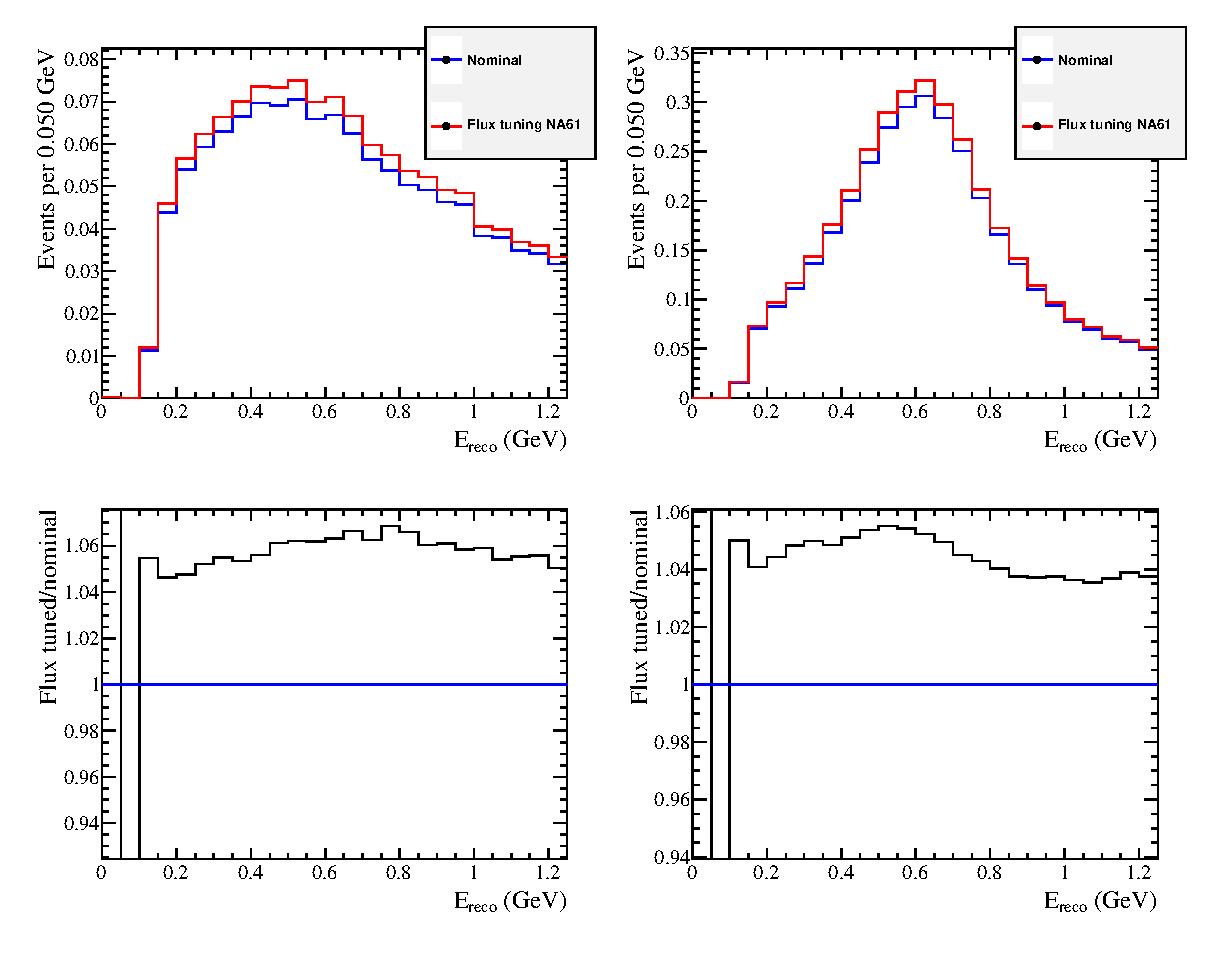
\includegraphics[width=30pc]{./nuebar_plots/spectrum_predictions/flux_tuning_effect.eps}
%\caption {
%    \huge{TO UPDATE} % caption is already ok
%{\large{SPECTRA NA61/SHINE TUNING MU-LIKE NEUTRINO MODE}}
%%Top: Reconstructed-energy spectrum of 1 $\mu$-like ring events in neutrino mode,
%%for an exposure 
%%of $6.914 \times 10^{20}$ POT %in neutrino mode
%%%and
%%%of $4.011 \times 10^{20}$ POT in antineutrino mode
%%both with and without the effect of the NA61/SHINE flux tuning of the nominal MC templates.
%%The spectra are shown both for no oscillations (left)
%%and for oscillations assuming the normal hierarchy, and the oscillation parameters shown in table~\ref{tab:osc_params_fixed_values_reactor}.
%%Bottom: Ratio of flux tuned with NA61/SHINE spectrum to the nominal MC spectrum.
%}
%\label{fig:1Rmu_spectrum_w_and_wo_na61_weights}
%\end{figure*}
%
%\begin{figure*}[htb]
%\center
%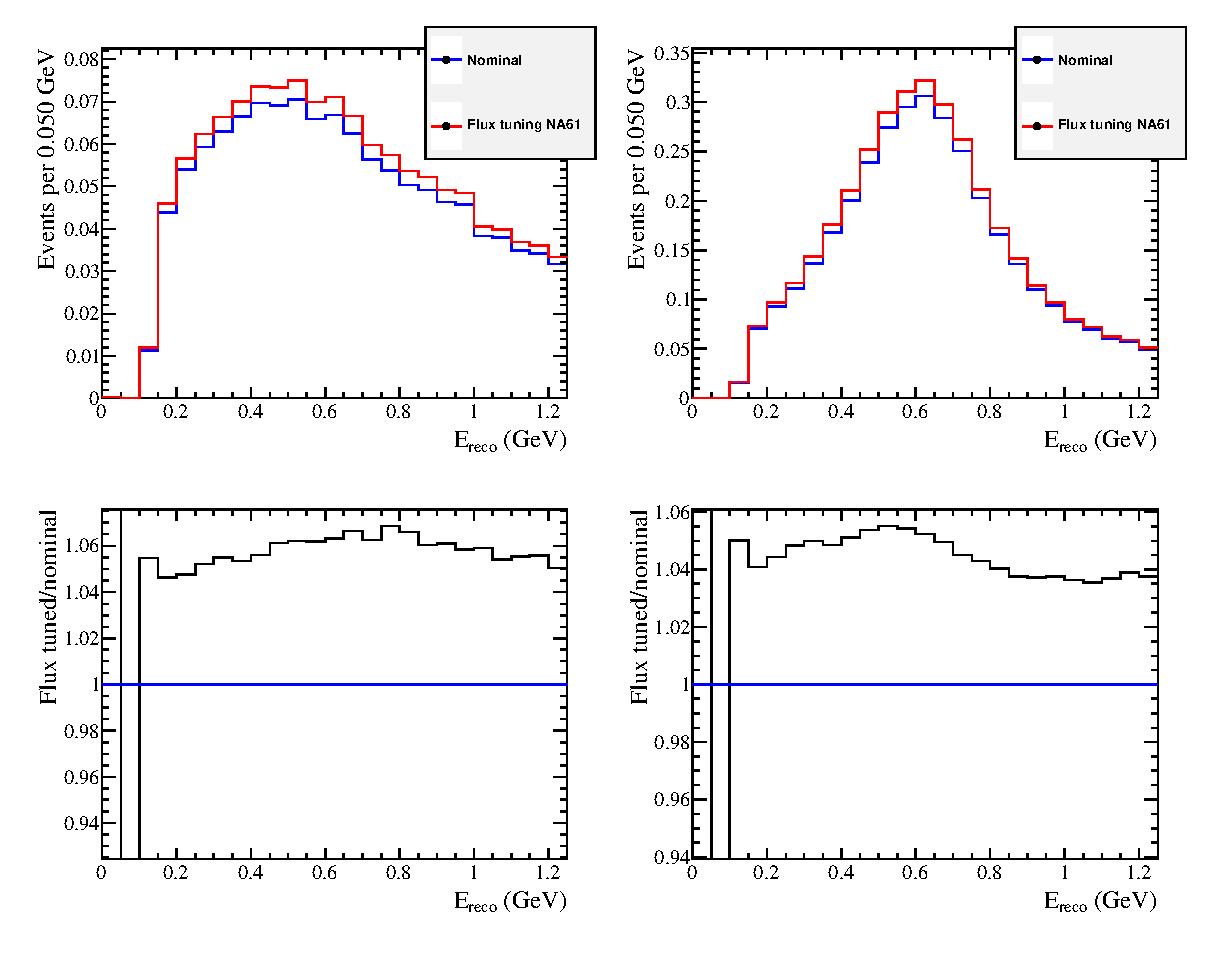
\includegraphics[width=30pc]{./nuebar_plots/spectrum_predictions/flux_tuning_effect.eps}
%\caption {
%    \huge{TO UPDATE} % caption is already ok
%{\large{SPECTRA NA61/SHINE TUNING MU-LIKE ANTINEUTRINO MODE}}
%%Top: Reconstructed-energy spectrum of 1 $\mu$-like ring events in antineutrino mode,
%%for an exposure 
%%%of $6.914 \times 10^{20}$ POT in neutrino mode
%%%and
%%of $4.011 \times 10^{20}$ POT% in antineutrino mode
%%both with and without the effect of the NA61/SHINE flux tuning of the nominal MC templates.
%%The spectra are shown both for no oscillations (left)
%%and for oscillations assuming the normal hierarchy, and the oscillation parameters shown in table~\ref{tab:osc_params_fixed_values_reactor}.
%%Bottom: Ratio of flux tuned with NA61/SHINE spectrum to the nominal MC spectrum.
%}
%\label{fig:RHC1Rmu_spectrum_w_and_wo_na61_weights}
%\end{figure*}
%
%\begin{figure*}[htb]
%\center
%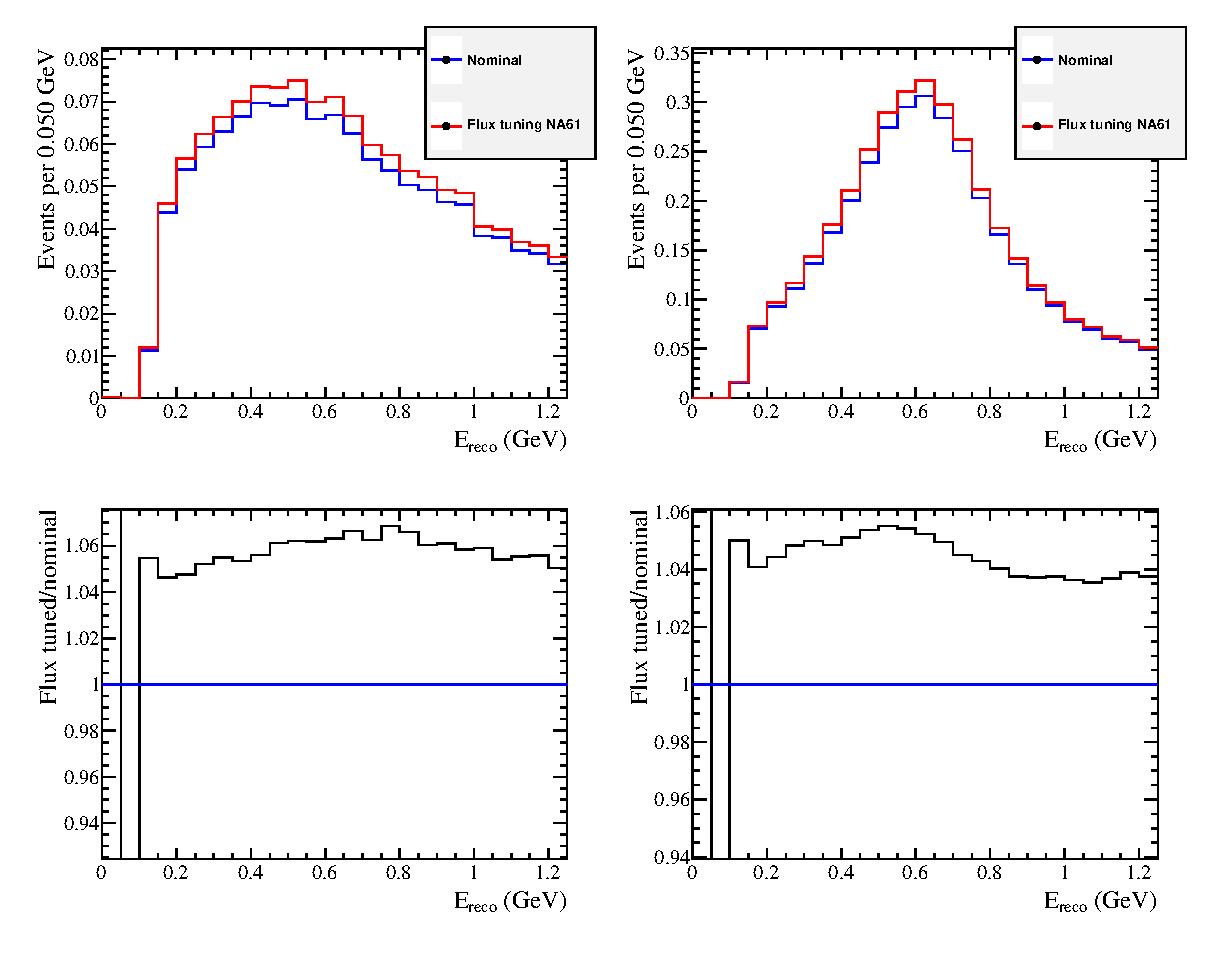
\includegraphics[width=30pc]{./nuebar_plots/spectrum_predictions/flux_tuning_effect.eps}
%\caption {
%    \huge{TO UPDATE} % caption is already ok
%{\large{SPECTRA NA61/SHINE TUNING E-LIKE NEUTRINO MODE}}
%%Top: Reconstructed-energy spectrum of 1 $e$-like ring events in neutrino mode,
%%for an exposure 
%%of $6.914 \times 10^{20}$ POT% in neutrino mode
%%%and
%%%of $4.011 \times 10^{20}$ POT in antineutrino mode
%%both with and without the effect of the NA61/SHINE flux tuning of the nominal MC templates.
%%The spectra are shown both for no oscillations (left)
%%and for oscillations assuming the normal hierarchy, and the oscillation parameters shown in table~\ref{tab:osc_params_fixed_values_reactor}.
%%Bottom: Ratio of flux tuned with NA61/SHINE spectrum to the nominal MC spectrum.
%}
%\label{fig:1Re_spectrum_w_and_wo_na61_weights}
%\end{figure*}
%
%\begin{figure*}[htb]
%\center
%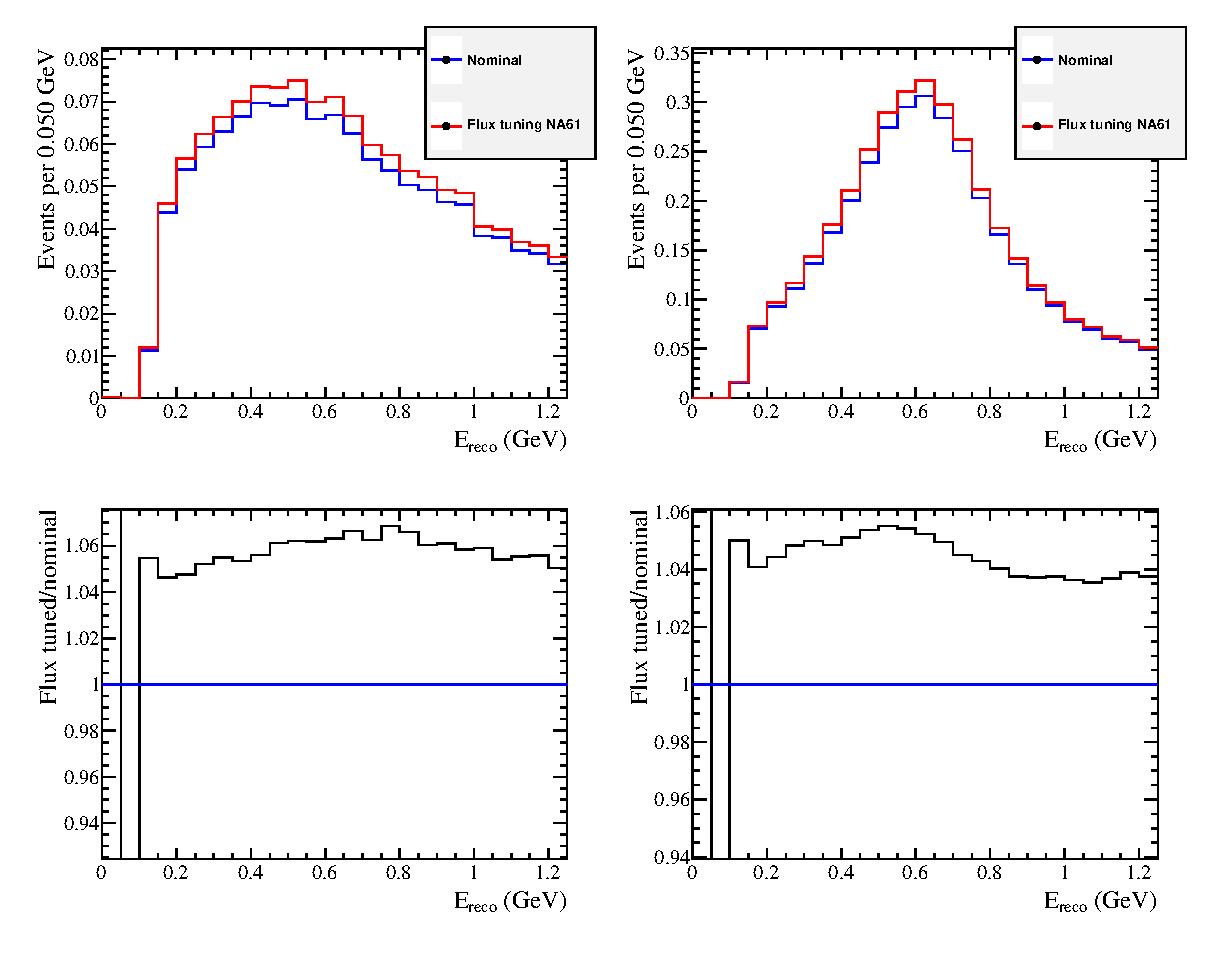
\includegraphics[width=30pc]{./nuebar_plots/spectrum_predictions/flux_tuning_effect.eps}
%\caption {
%    \huge{TO UPDATE} % caption is already ok
%{\large{SPECTRA NA61/SHINE TUNING E-LIKE ANTINEUTRINO MODE}}
%%Top: Reconstructed-energy spectrum of 1 $e$-like ring events in antineutrino mode,
%%for an exposure 
%%%of $6.914 \times 10^{20}$ POT in neutrino mode
%%%and
%%of $4.011 \times 10^{20}$ POT %in antineutrino mode
%%both with and without the effect of the NA61/SHINE flux tuning of the nominal MC templates.
%%The spectra are shown both for no oscillations (left)
%%and for oscillations assuming the normal hierarchy, and the oscillation parameters shown in table~\ref{tab:osc_params_fixed_values_reactor}.
%%Bottom: Ratio of flux tuned with NA61/SHINE spectrum to the nominal MC spectrum.
%}
%\label{fig:RHC1Re_spectrum_w_and_wo_na61_weights}
%\end{figure*}
%
%
%
%
%
%
%
%
%
%
%% Plots showing the effect of tunes on Ereco spectra w/ and w/o BANFF
%
%\begin{figure*}[htb]
%\center
%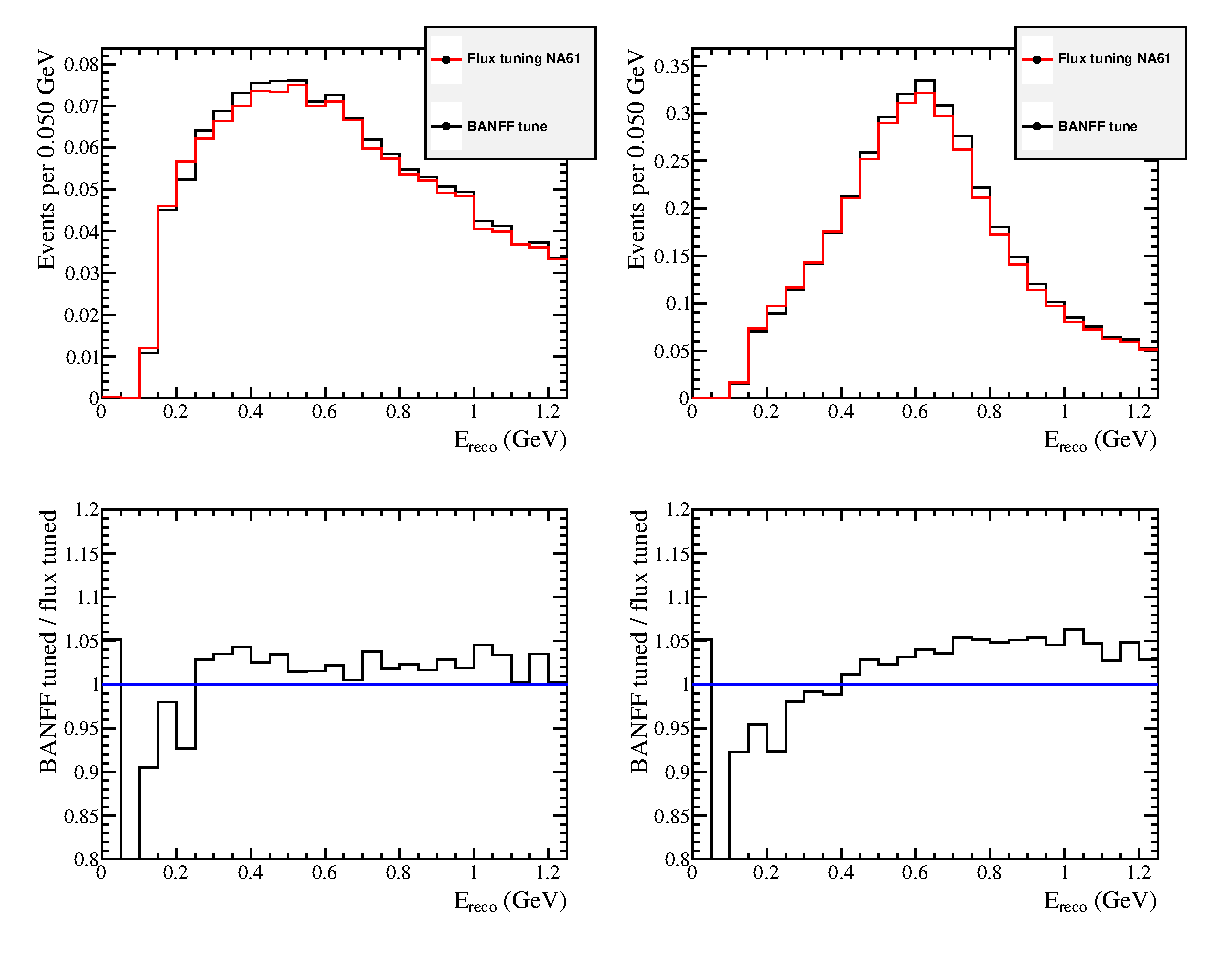
\includegraphics[width=30pc]{./nuebar_plots/spectrum_predictions/banff_tuning_effect.eps}
%\caption {
%    \huge{TO UPDATE} % caption is already ok
%{\large{SPECTRA BANFF TUNING MU-LIKE NEUTRINO MODE}}
%%Top: Reconstructed-energy spectrum of 1 $\mu$-like ring events in neutrino mode,
%%for an exposure 
%%of $6.914 \times 10^{20}$ POT % in neutrino mode
%%%and
%%%of $4.011 \times 10^{20}$ POT in antineutrino mode
%%both with and without the effect of postfit BANFF flux and cross-section tuning on the NA61/SHINE-tuned flux MC templates.
%%The spectra are shown both for no oscillations (left)
%%and for oscillations assuming the normal hierarchy, and the oscillation parameters shown in table~\ref{tab:osc_params_fixed_values_reactor}.
%%Bottom: Ratio of BANFF-tuned spectrum to the flux tuned with NA61/SHINE spectrum.
%}
%\label{fig:1Rmu_spectrum_w_and_wo_banff_weights}
%\end{figure*}
%
%\begin{figure*}[htb]
%\center
%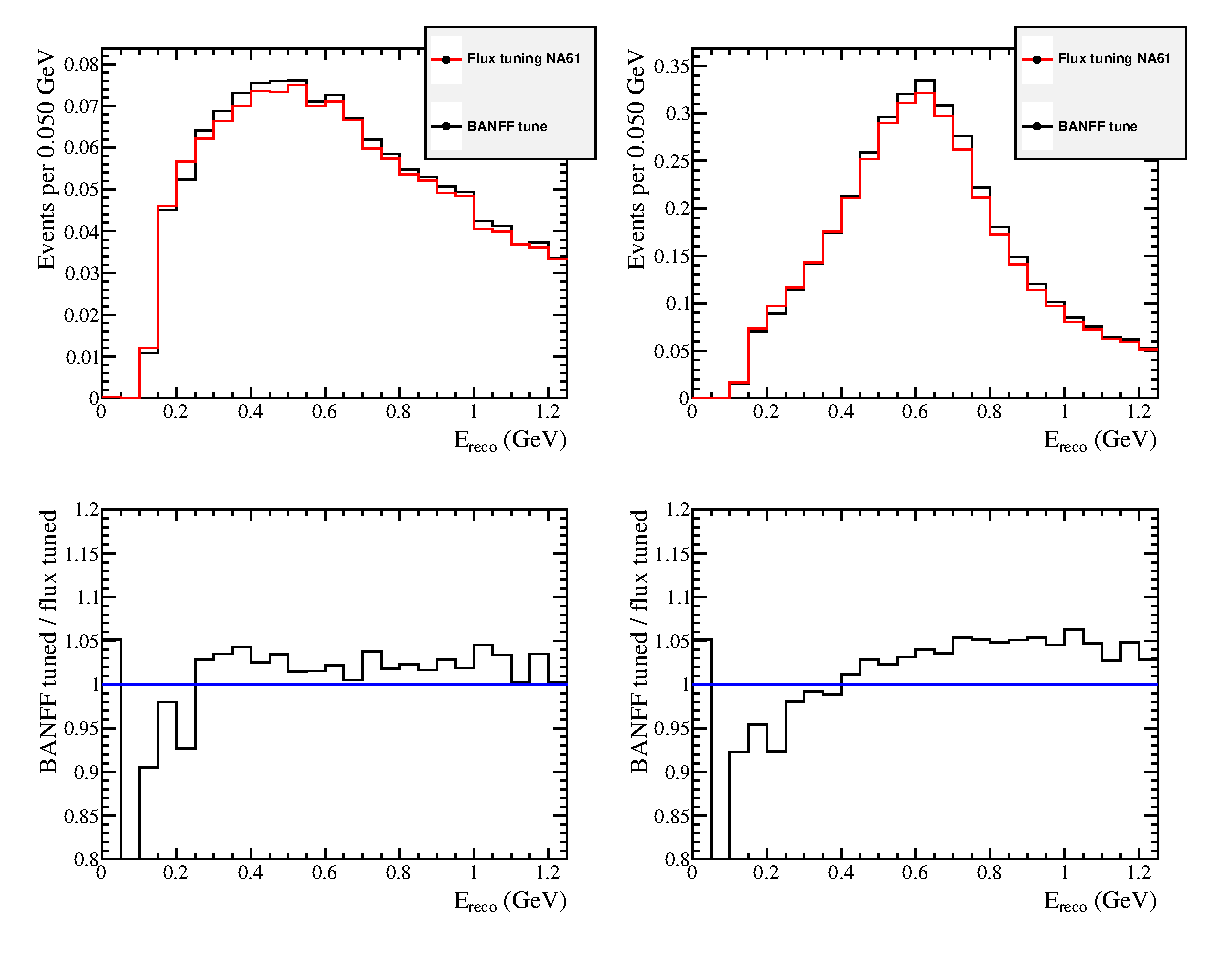
\includegraphics[width=30pc]{./nuebar_plots/spectrum_predictions/banff_tuning_effect.eps}
%\caption {
%    \huge{TO UPDATE} % caption is already ok
%{\large{SPECTRA BANFF TUNING MU-LIKE ANTINEUTRINO MODE}}
%%Top: Reconstructed-energy spectrum of 1 $\mu$-like ring events in antineutrino mode,
%%for an exposure 
%%%of $6.914 \times 10^{20}$ POT in neutrino mode
%%%and
%%of $4.011 \times 10^{20}$ POT% in antineutrino mode
%%both with and without the effect of postfit BANFF flux and cross-section tuning on the NA61/SHINE-tuned flux MC templates.
%%The spectra are shown both for no oscillations (left)
%%and for oscillations assuming the normal hierarchy, and the oscillation parameters shown in table~\ref{tab:osc_params_fixed_values_reactor}.
%%Bottom: Ratio of BANFF-tuned spectrum to the flux tuned with NA61/SHINE spectrum.
%}
%\label{fig:RHC1Rmu_spectrum_w_and_wo_banff_weights}
%\end{figure*}
%
%\begin{figure*}[htb]
%\center
%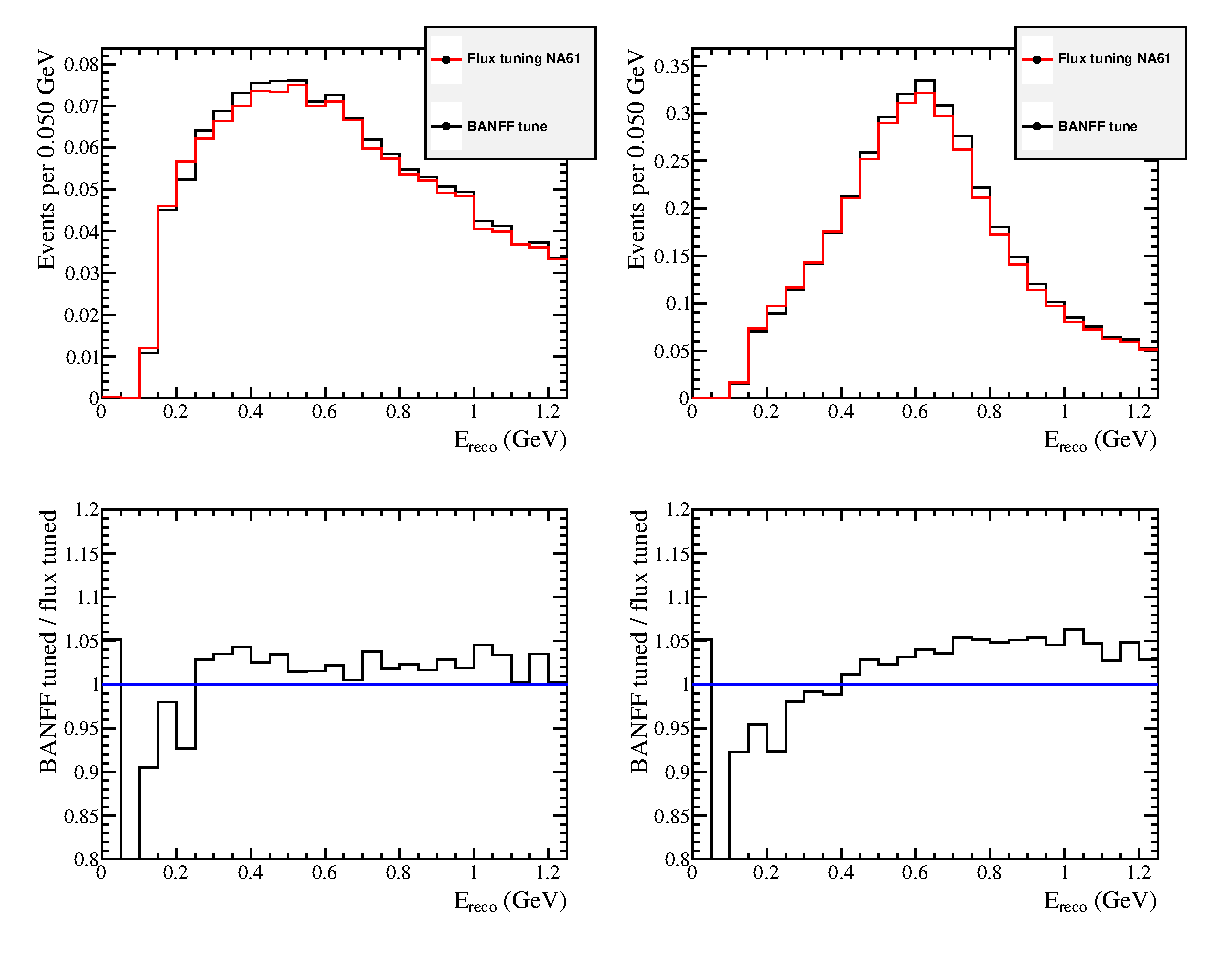
\includegraphics[width=30pc]{./nuebar_plots/spectrum_predictions/banff_tuning_effect.eps}
%\caption {
%    \huge{TO UPDATE} % caption is already ok
%{\large{SPECTRA BANFF TUNING E-LIKE NEUTRINO MODE}}
%%Top: Reconstructed-energy spectrum of 1 $e$-like ring events in neutrino mode,
%%for an exposure 
%%of $6.914 \times 10^{20}$ POT %in neutrino mode
%%%and
%%%of $4.011 \times 10^{20}$ POT in antineutrino mode
%%both with and without the effect of postfit BANFF flux and cross-section tuning on the NA61/SHINE-tuned flux MC templates.
%%The spectra are shown both for no oscillations (left)
%%and for oscillations assuming the normal hierarchy, and the oscillation parameters shown in table~\ref{tab:osc_params_fixed_values_reactor}.
%%Bottom: Ratio of BANFF-tuned spectrum to the flux tuned with NA61/SHINE spectrum.
%}
%\label{fig:1Re_spectrum_w_and_wo_banff_weights}
%\end{figure*}
%
%\begin{figure*}[htb]
%\center
%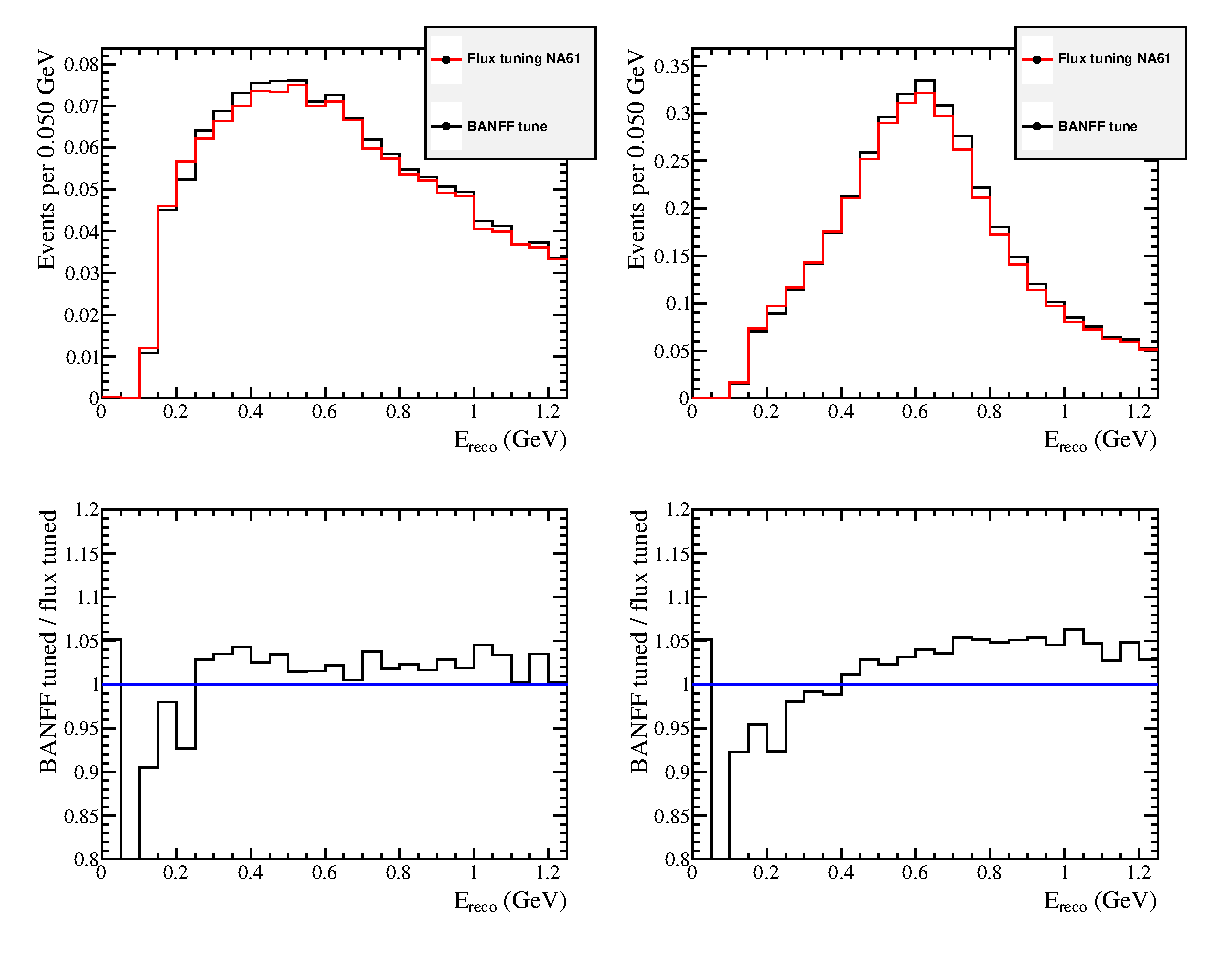
\includegraphics[width=30pc]{./nuebar_plots/spectrum_predictions/banff_tuning_effect.eps}
%\caption {
%    \huge{TO UPDATE} % caption is already ok
%{\large{SPECTRA BANFF TUNING E-LIKE ANTINEUTRINO MODE}}
%%Top: Reconstructed-energy spectrum of 1 $e$-like ring events in antineutrino mode,
%%for an exposure 
%%%of $6.914 \times 10^{20}$ POT in neutrino mode
%%%and
%%of $4.011 \times 10^{20}$ POT %in antineutrino mode
%%both with and without the effect of postfit BANFF flux and cross-section tuning on the NA61/SHINE-tuned flux MC templates.
%%The spectra are shown both for no oscillations (left)
%%and for oscillations assuming the normal hierarchy, and the oscillation parameters shown in table~\ref{tab:osc_params_fixed_values_reactor}.
%%Bottom: Ratio of BANFF-tuned spectrum to the flux tuned with NA61/SHINE spectrum.
%}
%\label{fig:RHC1Re_spectrum_w_and_wo_banff_weights}
%\end{figure*}
%
%\newpage
%\clearpage

In Tab.~\ref{tab:events_1rmu_Asimov_B},
\ref{tab:events_rhc1rmu_Asimov_B} and
\ref{tab:events_1re_Asimov_B},
\ref{tab:events_rhc1re_Asimov_B} 
the total number of events expected for the Asimov data set B (see \cref{tab:osc_params_joint_asimov}) is shown.

%\newpage
\clearpage


\begin{table}
\center
\begin{tabular} { | l ||r | r | r | r | r | r | | r | }
\hline
              & $\nu_\mu$            & $\nu_e$              & $\bar{\nu_\mu}$      & $\bar{\nu_e}$        & Osc. $\nu_e$         & Osc. $\bar{\nu_e}$   & Total                \\ \hline\hline
 CCQE         & 69.747               & 0.035                & 4.335                & 0.002                & 0.151                & 0.001                & 74.270               \\ \hline
 CC1pi        & 17.206               & 0.017                & 1.572                & 0.001                & 0.049                & 0.000                & 18.845               \\ \hline
 CCcoherent   & 0.330                & 0.000                & 0.080                & 0.000                & 0.001                & 0.000                & 0.412                \\ \hline
 2p-2h          & 19.725               & 0.010                & 0.852                & 0.000                & 0.036                & 0.000                & 20.623               \\ \hline
 CCother      & 7.742                & 0.008                & 0.494                & 0.001                & 0.002                & 0.000                & 8.247                \\ \hline
 NC1pi0       & 0.537                & 0.016                & 0.017                & 0.001                & N/A                  & N/A                  & 0.572                \\ \hline
 NC1piPM      & 3.944                & 0.089                & 0.142                & 0.008                & N/A                  & N/A                  & 4.183                \\ \hline
 NCcoherent   & 0.016                & 0.000                & 0.001                & 0.000                & N/A                  & N/A                  & 0.018                \\ \hline
 NCother      & 2.993                & 0.121                & 0.165                & 0.012                & N/A                  & N/A                  & 3.290                \\ \hline
 NC1gamma     & 0.004                & 0.000                & 0.000                & 0.000                & N/A                  & N/A                  & 0.004                \\ \hline
\hline
 Total        & 122.243              & 0.297                & 7.659                & 0.025                & 0.238                & 0.002                & 130.464              \\ \hline
\end{tabular}
\caption{
%{\Huge{TO UPDATE}}
Predicted number of events in the neutrino mode $\mu$-like sample
obtained after applying the BANFF weight
for a total exposure of \TotalPotNu{} POT.
The Asimov data set B in \cref{tab:osc_params_joint_asimov} is used.
}
\label{tab:events_1rmu_Asimov_B}
\end{table}




\begin{table}
\center
\begin{tabular} { | l ||r | r | r | r | r | r | | r | }
\hline
             & $\nu_\mu$            & $\nu_e$              & $\bar{\nu_\mu}$      & $\bar{\nu_e}$        & Osc. $\nu_e$         & Osc. $\bar{\nu_e}$   & Total                \\ \hline\hline
 CCQE         & 7.088                & 0.004                & 13.306               & 0.005                & 0.004                & 0.016                & 20.422               \\ \hline
 CC1pi        & 2.718                & 0.003                & 3.066                & 0.002                & 0.002                & 0.003                & 5.794                \\ \hline
 CCcoherent   & 0.054                & 0.000                & 0.173                & 0.000                & 0.000                & 0.000                & 0.228                \\ \hline
 2p-2h          & 2.525                & 0.001                & 2.118                & 0.001                & 0.001                & 0.002                & 4.649                \\ \hline
 CCother      & 1.282                & 0.001                & 0.886                & 0.000                & 0.000                & 0.000                & 2.170                \\ \hline
 NC1pi0       & 0.060                & 0.002                & 0.050                & 0.001                & N/A                  & N/A                  & 0.114                \\ \hline
 NC1piPM      & 0.378                & 0.015                & 0.380                & 0.010                & N/A                  & N/A                  & 0.784                \\ \hline
 NCcoherent   & 0.001                & 0.000                & 0.006                & 0.000                & N/A                  & N/A                  & 0.008                \\ \hline
 NCother      & 0.530                & 0.025                & 0.296                & 0.012                & N/A                  & N/A                  & 0.862                \\ \hline
 NC1gamma     & 0.000                & 0.000                & 0.000                & 0.000                & N/A                  & N/A                  & 0.000                \\ \hline
\hline
 Total        & 14.637               & 0.051                & 20.282               & 0.032                & 0.008                & 0.022                & 35.032               \\ \hline

\end{tabular}
\caption{
%{\Huge{TO UPDATE}}
Predicted number of events in the antineutrino mode $\mu$-like sample
obtained after applying the BANFF weight
for a total exposure of \TotalPotNuBar{} POT.
The Asimov data set B in \cref{tab:osc_params_joint_asimov} is used.
}
\label{tab:events_rhc1rmu_Asimov_B}
\end{table}




\begin{table}
\center
\begin{tabular} { | l ||r | r | r | r | r | r | | r | }
\hline
              & $\nu_\mu$            & $\nu_e$              & $\bar{\nu_\mu}$      & $\bar{\nu_e}$        & Osc. $\nu_e$         & Osc. $\bar{\nu_e}$   & Total                \\ \hline\hline
 CCQE         & 0.062                & 2.129                & 0.001                & 0.088                & 10.811               & 0.121                & 13.211               \\ \hline
 CC1pi        & 0.017                & 0.348                & 0.000                & 0.027                & 1.236                & 0.020                & 1.648                \\ \hline
 CCcoherent   & 0.000                & 0.002                & 0.000                & 0.002                & 0.011                & 0.002                & 0.017                \\ \hline
 2p-2h          & 0.009                & 0.710                & 0.000                & 0.022                & 2.750                & 0.022                & 3.513                \\ \hline
 CCother      & 0.001                & 0.045                & 0.000                & 0.003                & 0.025                & 0.001                & 0.076                \\ \hline
 NC1pi0       & 0.524                & 0.012                & 0.017                & 0.001                & N/A                  & N/A                  & 0.553                \\ \hline
 NC1piPM      & 0.099                & 0.002                & 0.003                & 0.000                & N/A                  & N/A                  & 0.105                \\ \hline
 NCcoherent   & 0.174                & 0.004                & 0.018                & 0.001                & N/A                  & N/A                  & 0.197                \\ \hline
 NCother      & 0.126                & 0.005                & 0.008                & 0.001                & N/A                  & N/A                  & 0.139                \\ \hline
 NC1gamma     & 0.464                & 0.007                & 0.021                & 0.001                & N/A                  & N/A                  & 0.494                \\ \hline
\hline
 Total        & 1.476                & 3.264                & 0.069                & 0.145                & 14.833               & 0.167                & 19.954               \\ \hline

\end{tabular}
\caption{
%{\Huge{TO UPDATE}}
Predicted number of events in the neutrino mode $e$-like sample
obtained after applying the BANFF weight
for a total exposure of \TotalPotNu{} POT.
The Asimov data set B in \cref{tab:osc_params_joint_asimov} is used.
}
\label{tab:events_1re_Asimov_B}
\end{table}




\begin{table}
\center
\begin{tabular} { | l ||r | r | r | r | r | r | | r | }
\hline
              & $\nu_\mu$            & $\nu_e$              & $\bar{\nu_\mu}$      & $\bar{\nu_e}$        & Osc. $\nu_e$         & Osc. $\bar{\nu_e}$   & Total                \\ \hline\hline
 CCQE         & 0.002                & 0.189                & 0.003                & 0.339                & 0.269                & 1.376                & 2.178                \\ \hline
 CC1pi        & 0.002                & 0.040                & 0.001                & 0.060                & 0.045                & 0.163                & 0.312                \\ \hline
 CCcoherent   & 0.000                & 0.000                & 0.000                & 0.006                & 0.000                & 0.022                & 0.029                \\ \hline
 2p-2h          & 0.001                & 0.069                & 0.000                & 0.063                & 0.087                & 0.219                & 0.439                \\ \hline
 CCother      & 0.001                & 0.008                & 0.000                & 0.004                & 0.003                & 0.003                & 0.019                \\ \hline
 NC1pi0       & 0.045                & 0.002                & 0.049                & 0.001                & N/A                  & N/A                  & 0.098                \\ \hline
 NC1piPM      & 0.011                & 0.000                & 0.008                & 0.000                & N/A                  & N/A                  & 0.020                \\ \hline
 NCcoherent   & 0.021                & 0.001                & 0.081                & 0.001                & N/A                  & N/A                  & 0.103                \\ \hline
 NCother      & 0.022                & 0.001                & 0.012                & 0.000                & N/A                  & N/A                  & 0.035                \\ \hline
 NC1gamma     & 0.037                & 0.002                & 0.081                & 0.002                & N/A                  & N/A                  & 0.121                \\ \hline
\hline
 Total        & 0.142                & 0.313                & 0.235                & 0.478                & 0.404                & 1.783                & 3.355                \\ \hline

\end{tabular}
\caption{
%{\Huge{TO UPDATE}}
Predicted number of events in the antineutrino mode $\mu$-like sample
obtained after applying the BANFF weight
for a total exposure of \TotalPotNuBar{} POT.
The Asimov data set B in \cref{tab:osc_params_joint_asimov} is used.
}
\label{tab:events_rhc1re_Asimov_B}
\end{table}





\newpage
\clearpage

In Tab.~\ref{tab:events_1rmu_NoOsc},
\ref{tab:events_rhc1rmu_NoOsc} and
\ref{tab:events_1re_NoOsc},
\ref{tab:events_rhc1re_NoOsc}
the total number of unoscillated events is shown.
 

\begin{table}
\center
\begin{tabular} { | l ||r | r | r | r | r | r | | r | }
\hline
              & $\nu_\mu$            & $\nu_e$              & $\bar{\nu_\mu}$      & $\bar{\nu_e}$        & Osc. $\nu_e$         & Osc. $\bar{\nu_e}$   & Total                \\ \hline\hline
 CCQE         & 338.683              & 0.037                & 8.672                & 0.002                & 0.000                & 0.000                & 347.394              \\ \hline
 CC1pi        & 39.668               & 0.018                & 2.276                & 0.001                & 0.000                & 0.000                & 41.963               \\ \hline
 CCcoherent   & 0.678                & 0.000                & 0.136                & 0.000                & 0.000                & 0.000                & 0.815                \\ \hline
 2p-2h          & 74.638               & 0.011                & 1.548                & 0.000                & 0.000                & 0.000                & 76.198               \\ \hline
 CCother      & 8.732                & 0.009                & 0.560                & 0.001                & 0.000                & 0.000                & 9.301                \\ \hline
 NC1pi0       & 0.537                & 0.016                & 0.017                & 0.001                & N/A                  & N/A                  & 0.572                \\ \hline
 NC1piPM      & 3.944                & 0.089                & 0.142                & 0.008                & N/A                  & N/A                  & 4.183                \\ \hline
 NCcoherent   & 0.016                & 0.000                & 0.001                & 0.000                & N/A                  & N/A                  & 0.018                \\ \hline
 NCother      & 2.993                & 0.121                & 0.165                & 0.012                & N/A                  & N/A                  & 3.290                \\ \hline
 NC1gamma     & 0.004                & 0.000                & 0.000                & 0.000                & N/A                  & N/A                  & 0.004                \\ \hline
\hline
 Total        & 469.893              & 0.301                & 13.518               & 0.025                & 0.000                & 0.000                & 483.737              \\ \hline
\end{tabular}
\caption{
%{\Huge{TO UPDATE}}
Predicted number of events in the neutrino mode $\mu$-like sample
obtained after applying the BANFF weight
for a total exposure of \TotalPotNu{} POT.
Oscillations are not applied.
}
\label{tab:events_1rmu_NoOsc}
\end{table}




\begin{table}
\center
\begin{tabular} { | l ||r | r | r | r | r | r | | r | }
\hline
              & $\nu_\mu$            & $\nu_e$              & $\bar{\nu_\mu}$      & $\bar{\nu_e}$        & Osc. $\nu_e$         & Osc. $\bar{\nu_e}$   & Total                \\ \hline\hline
 CCQE         & 15.420               & 0.004                & 55.525               & 0.005                & 0.000                & 0.000                & 70.954               \\ \hline
 CC1pi        & 4.071                & 0.003                & 6.536                & 0.002                & 0.000                & 0.000                & 10.611               \\ \hline
 CCcoherent   & 0.074                & 0.000                & 0.612                & 0.000                & 0.000                & 0.000                & 0.687                \\ \hline
 2p-2h          & 4.721                & 0.001                & 7.811                & 0.001                & 0.000                & 0.000                & 12.534               \\ \hline
 CCother      & 1.457                & 0.001                & 1.008                & 0.000                & 0.000                & 0.000                & 2.467                \\ \hline
 NC1pi0       & 0.060                & 0.002                & 0.050                & 0.001                & N/A                  & N/A                  & 0.114                \\ \hline
 NC1piPM      & 0.378                & 0.015                & 0.380                & 0.010                & N/A                  & N/A                  & 0.784                \\ \hline
 NCcoherent   & 0.001                & 0.000                & 0.006                & 0.000                & N/A                  & N/A                  & 0.008                \\ \hline
 NCother      & 0.530                & 0.025                & 0.296                & 0.012                & N/A                  & N/A                  & 0.862                \\ \hline
 NC1gamma     & 0.000                & 0.000                & 0.000                & 0.000                & N/A                  & N/A                  & 0.000                \\ \hline
\hline
 Total        & 26.713               & 0.052                & 72.225               & 0.032                & 0.000                & 0.000                & 99.021               \\ \hline

\end{tabular}
\caption{
%{\Huge{TO UPDATE}}
Predicted number of events in the antineutrino mode $\mu$-like sample
obtained after applying the BANFF weight
for a total exposure of \TotalPotNuBar{} POT.
Oscillations are not applied.
}
\label{tab:events_rhc1rmu_NoOsc}
\end{table}




\begin{table}
\center
\begin{tabular} { | l ||r | r | r | r | r | r | | r | }
\hline
               & $\nu_\mu$            & $\nu_e$              & $\bar{\nu_\mu}$      & $\bar{\nu_e}$        & Osc. $\nu_e$         & Osc. $\bar{\nu_e}$   & Total                \\ \hline\hline
 CCQE         & 0.413                & 2.294                & 0.002                & 0.094                & 0.000                & 0.000                & 2.803                \\ \hline
 CC1pi        & 0.069                & 0.371                & 0.001                & 0.028                & 0.000                & 0.000                & 0.469                \\ \hline
 CCcoherent   & 0.002                & 0.003                & 0.000                & 0.002                & 0.000                & 0.000                & 0.006                \\ \hline
 2p-2h          & 0.095                & 0.759                & 0.000                & 0.023                & 0.000                & 0.000                & 0.878                \\ \hline
 CCother      & 0.004                & 0.046                & 0.000                & 0.003                & 0.000                & 0.000                & 0.054                \\ \hline
 NC1pi0       & 0.524                & 0.012                & 0.017                & 0.001                & N/A                  & N/A                  & 0.553                \\ \hline
 NC1piPM      & 0.099                & 0.002                & 0.003                & 0.000                & N/A                  & N/A                  & 0.105                \\ \hline
 NCcoherent   & 0.174                & 0.004                & 0.018                & 0.001                & N/A                  & N/A                  & 0.197                \\ \hline
 NCother      & 0.126                & 0.005                & 0.008                & 0.001                & N/A                  & N/A                  & 0.139                \\ \hline
 NC1gamma     & 0.464                & 0.007                & 0.021                & 0.001                & N/A                  & N/A                  & 0.494                \\ \hline
\hline
 Total        & 1.970                & 3.504                & 0.071                & 0.154                & 0.000                & 0.000                & 5.698                \\ \hline

\end{tabular}
\caption{
%{\Huge{TO UPDATE}}
Predicted number of events in the neutrino mode $e$-like sample
obtained after applying the BANFF weight
for a total exposure of \TotalPotNu{} POT.
Oscillations are not applied.
}
\label{tab:events_1re_NoOsc}
\end{table}




\begin{table}
\center
\begin{tabular} { | l ||r | r | r | r | r | r | | r | }
\hline
              & $\nu_\mu$            & $\nu_e$              & $\bar{\nu_\mu}$      & $\bar{\nu_e}$        & Osc. $\nu_e$         & Osc. $\bar{\nu_e}$   & Total                \\ \hline\hline
 CCQE         & 0.012                & 0.203                & 0.018                & 0.361                & 0.000                & 0.000                & 0.593                \\ \hline
 CC1pi        & 0.004                & 0.043                & 0.003                & 0.064                & 0.000                & 0.000                & 0.114                \\ \hline
 CCcoherent   & 0.000                & 0.000                & 0.000                & 0.006                & 0.000                & 0.000                & 0.007                \\ \hline
 2p-2h          & 0.003                & 0.074                & 0.003                & 0.067                & 0.000                & 0.000                & 0.147                \\ \hline
 CCother      & 0.001                & 0.009                & 0.000                & 0.004                & 0.000                & 0.000                & 0.015                \\ \hline
 NC1pi0       & 0.045                & 0.002                & 0.049                & 0.001                & N/A                  & N/A                  & 0.098                \\ \hline
 NC1piPM      & 0.011                & 0.000                & 0.008                & 0.000                & N/A                  & N/A                  & 0.020                \\ \hline
 NCcoherent   & 0.021                & 0.001                & 0.081                & 0.001                & N/A                  & N/A                  & 0.103                \\ \hline
 NCother      & 0.022                & 0.001                & 0.012                & 0.000                & N/A                  & N/A                  & 0.035                \\ \hline
 NC1gamma     & 0.037                & 0.002                & 0.081                & 0.002                & N/A                  & N/A                  & 0.121                \\ \hline
\hline
 Total        & 0.156                & 0.334                & 0.255                & 0.507                & 0.000                & 0.000                & 1.253                \\ \hline

\end{tabular}
\caption{
%{\Huge{TO UPDATE}}
Predicted number of events in the antineutrino mode $e$-like sample
obtained after applying the BANFF weight
for a total exposure of \TotalPotNuBar{} POT.
Oscillations are not applied.
}
\label{tab:events_rhc1re_NoOsc}
\end{table}





\clearpage







%...........................................................
%
% Predicted spectra
%
%...........................................................

\section{Predicted $e$-like spectra}
\label{app:templates_elike}

In Fig.~\ref{fig:joint_ereco_components} each flavor component 
of the neutrino and antineutrino mode $e$-like samples
is shown separately in order to compare the different shapes as a function of $E_{reco}$.
The NC spectrum distribution,
which is the largest component of the background,
is quite flat over all the energy range and is quite difficult to separate.
The $\nu_{\mu} \rightarrow \nu_e$ and $\bar{\nu}_{\mu} \rightarrow \bar{\nu}_e$ events
populate the same energy region, around 0.6 GeV, with a very similar shape.

\begin{figure*}[htb]
%\hspace{0.06\linewidth}
\center
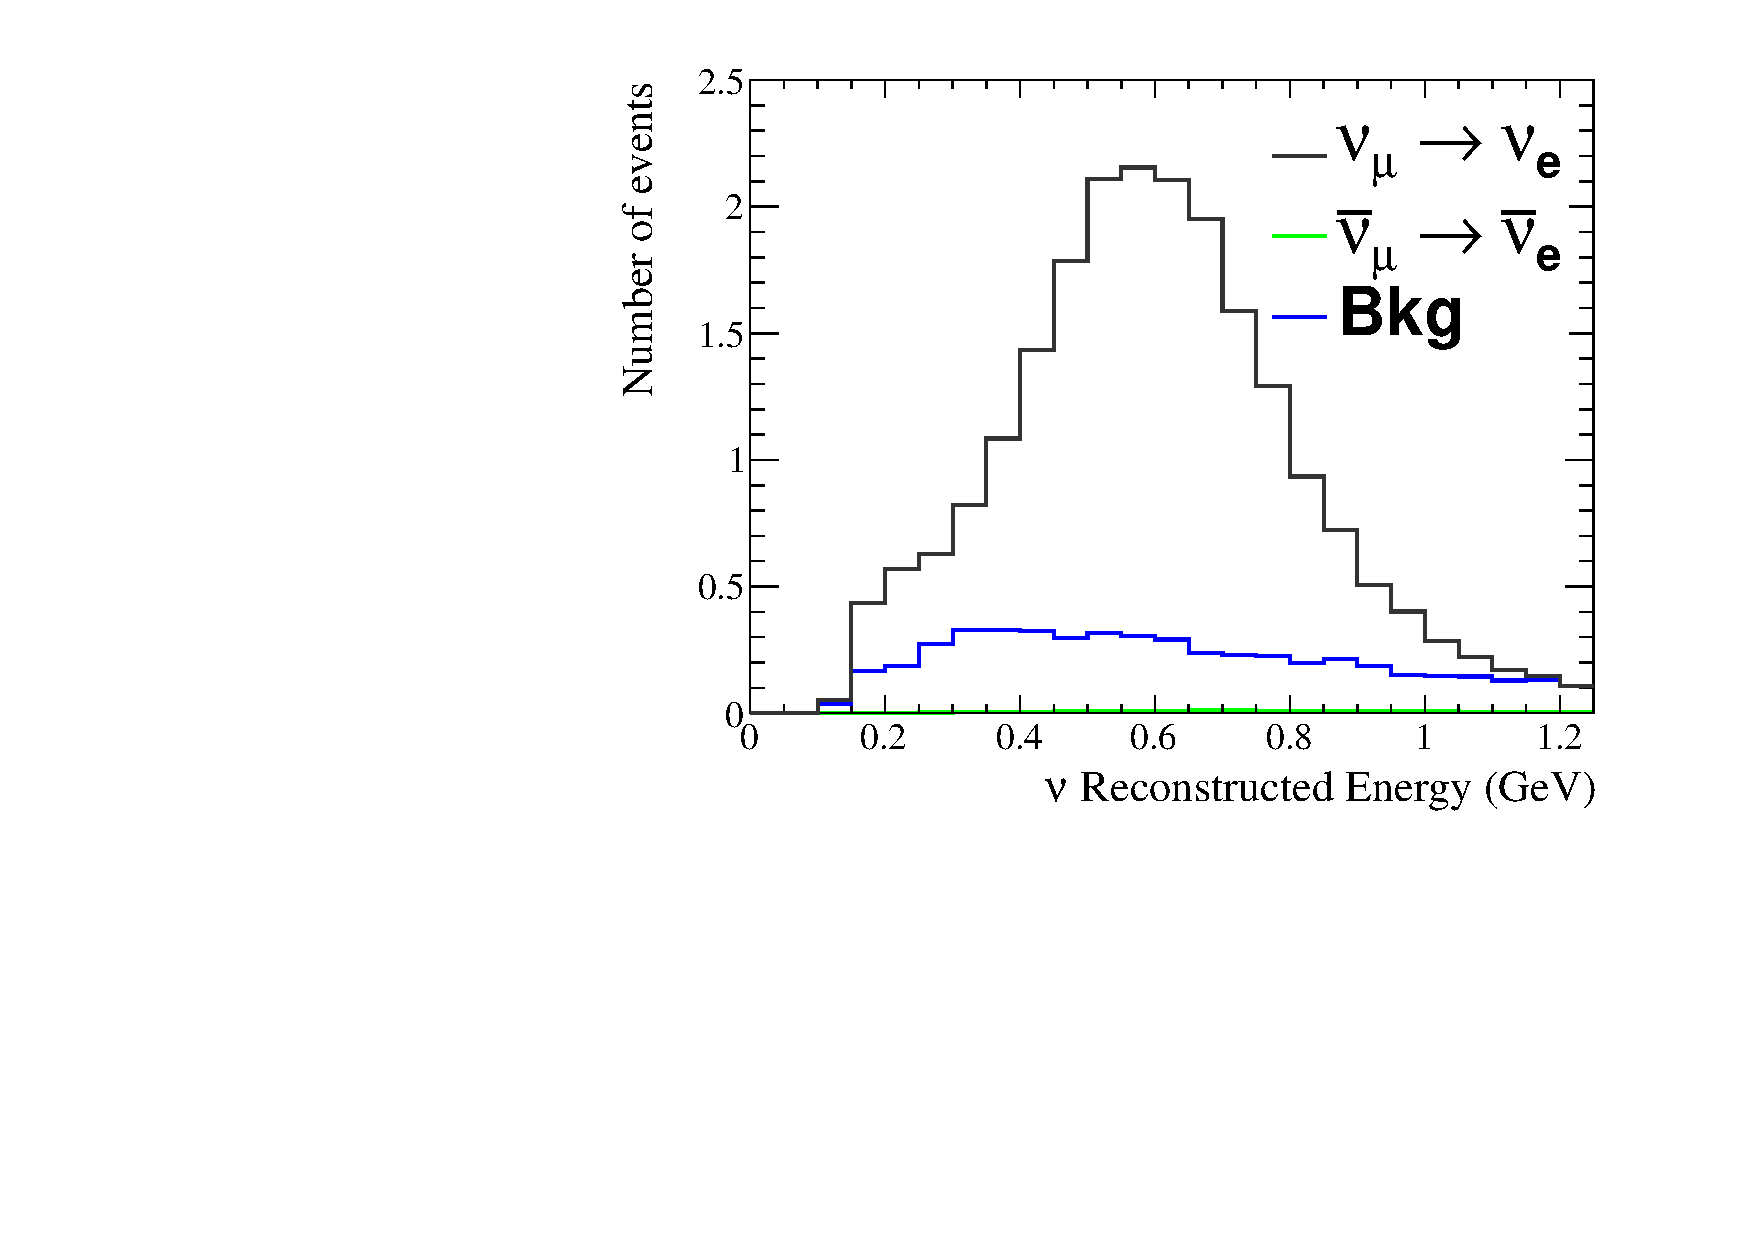
\includegraphics[width=18pc]{joint_plots/spectrum_predictions/template_ereco_1re_component.pdf}
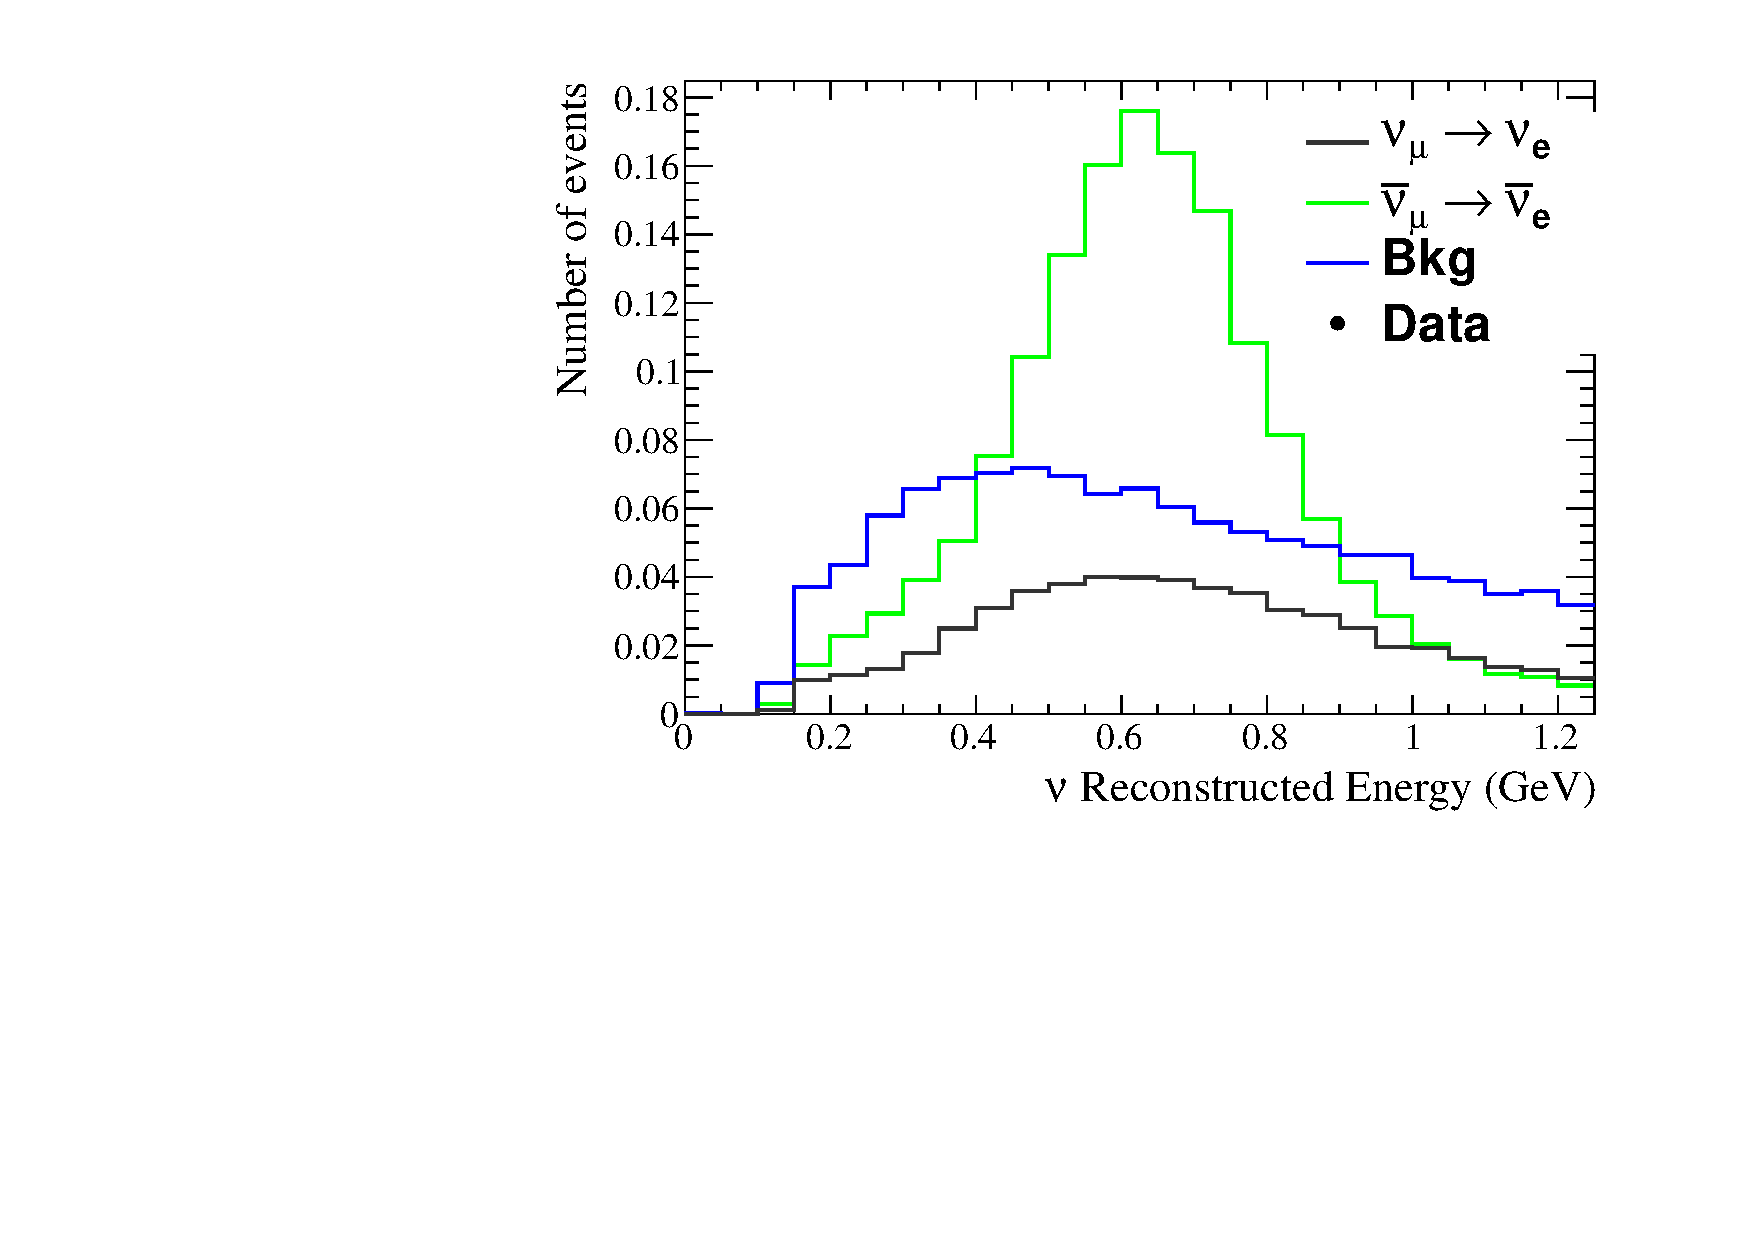
\includegraphics[width=18pc]{joint_plots/spectrum_predictions/template_ereco_rhc1re_component.pdf}
\caption {
  %  \huge{TO UPDATE} % caption is already ok
%{\large{ERECO SPECTRA WITH SEPARATED COMPONENTS}}
Predicted spectra of reconstructed neutrino energy 
for electron-like 
neutrino mode (left)
and
antineutrino mode (right)
events.
The distributions correspond to the collected statistics in the full Run 1-6 data set
for an exposure 
of $6.914 \times 10^{20}$ POT in neutrino mode
and
of $4.011 \times 10^{20}$ POT in antineutrino mode.
The distributions are broken down by the following components:
$\bar{\nu}_{\mu} \to \bar{\nu}_e$ (green), 
$\nu_{\mu} \to \nu_e$ (black/white), 
background, 
which includes 
NC,
$\nu_e + \bar{\nu}_e$ intrinsic beam (yellow),
$\nu_{\mu}$ intrinsic beam (light blue)
and
$\bar{\nu}_{\mu}$ intrinsic beam (blue).
The spectra were generated with the systematic parameters measured with the ND280 data 
shown in tab.~\ref{tab:banff_uncertainties_flux_fhc},~\ref{tab:banff_uncertainties_flux_rhc},~\ref{tab:banff_uncertainties_xsec}
and \ref{tab:banff_uncertainties_skdetfsi}
and the oscillation parameters corresponding to the Asimov data set A shown in tab.~\ref{tab:osc_params_joint_asimov}.
%The predicted spectrum of antineutrino mode 
%is scaled by a factor 7.
}
\label{fig:joint_ereco_components}
\end{figure*}


Another kinematical variable is thus needed in order to better separate different flavour / reaction compoonents.
In Fig.~\ref{fig:joint_ereco_vs_theta_1re} and~\ref{fig:joint_ereco_vs_theta_rhc1re}
the 2-dimensional $E_{reco}$ Vs $\theta$ spectra are shown for each flavour component and NC
for both neutrino and antineutrino mode $e$-like samples.
In particular the shapes of $\nu_{\mu} \rightarrow \nu_e$ and $\bar{\nu}_{\mu} \rightarrow \bar{\nu}_e$ 
distributions are quite different, thus this templates have a better capability to 
discriminate signal from background.
In general this template parametrization produces quite different shapes for all the flavour and NC components.

\begin{figure*}[htb]
%\hspace{0.06\linewidth}
\center
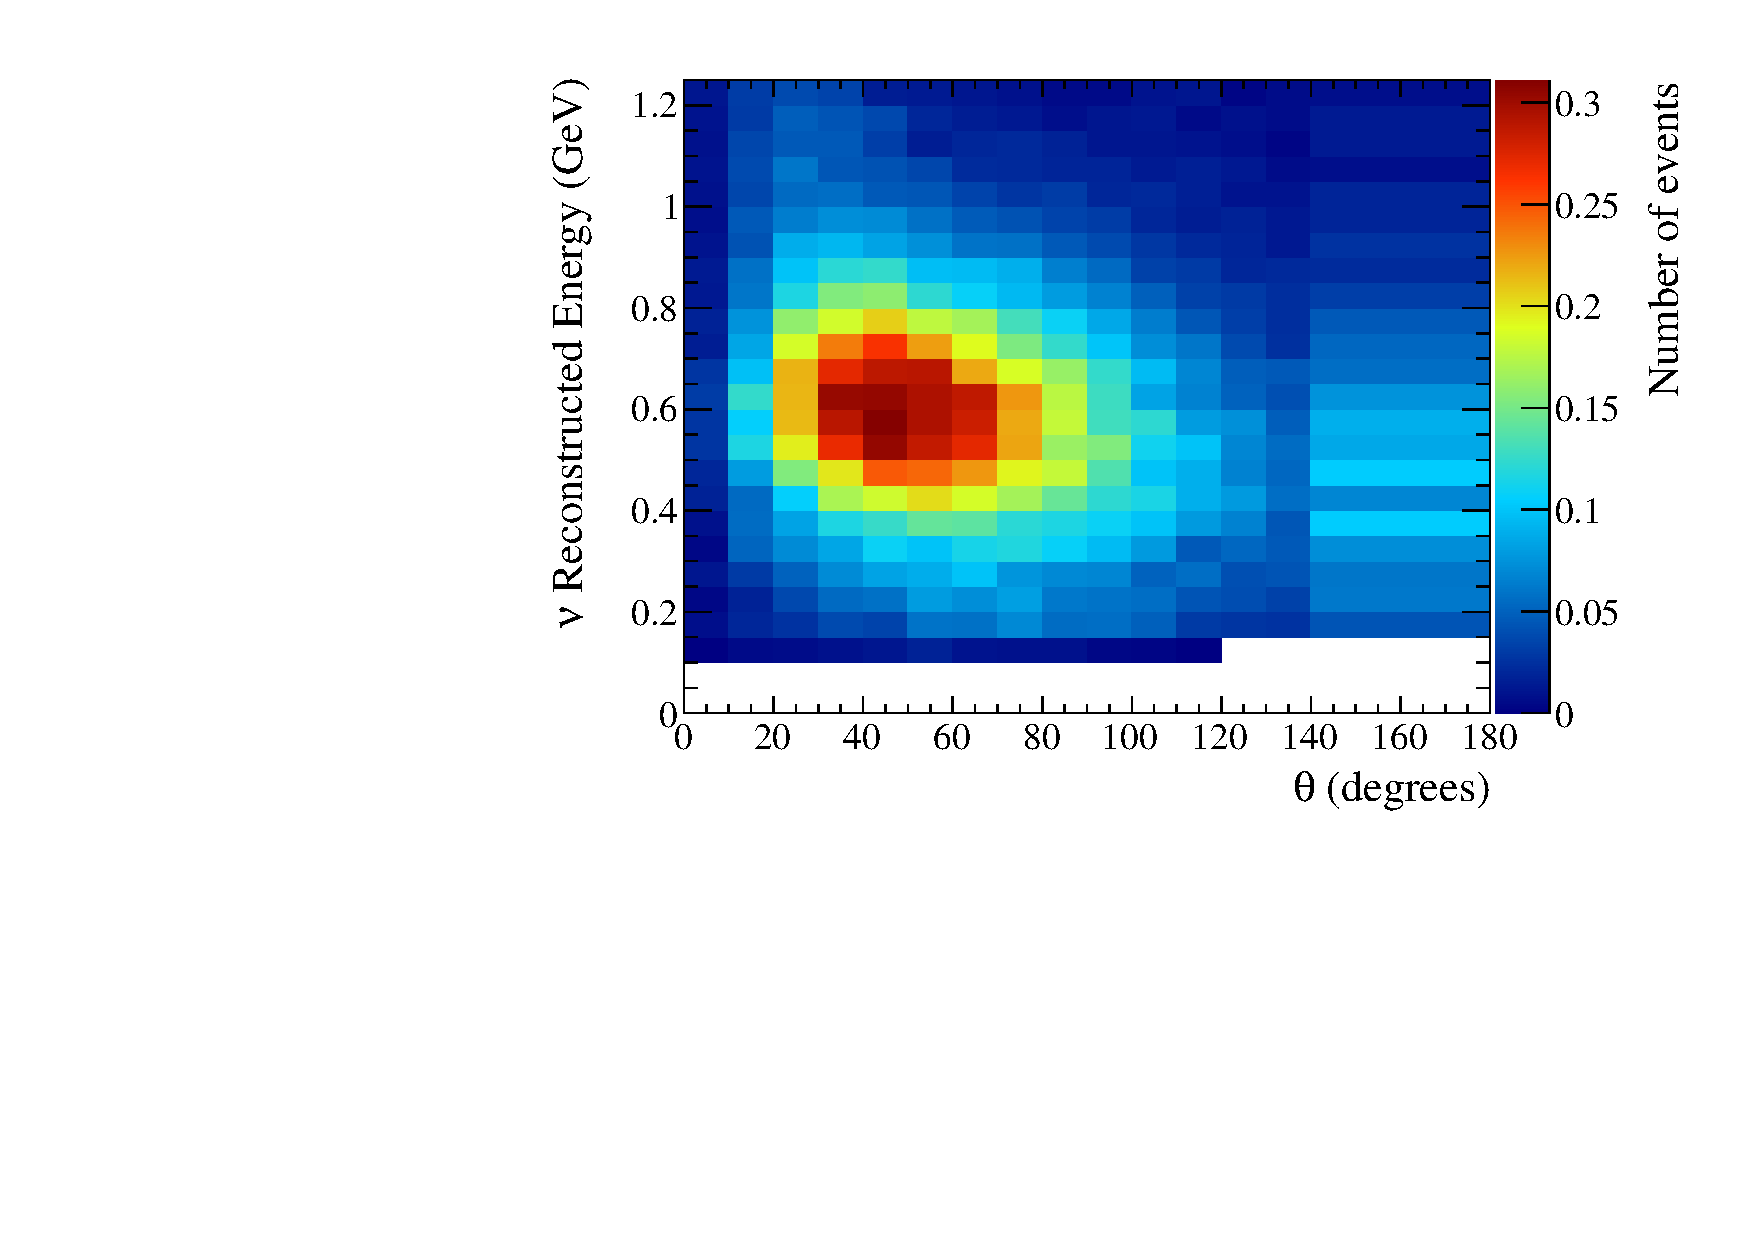
\includegraphics[width=18pc]{joint_plots/spectrum_predictions/template_ereco_vs_theta_tot_1re.pdf}\\
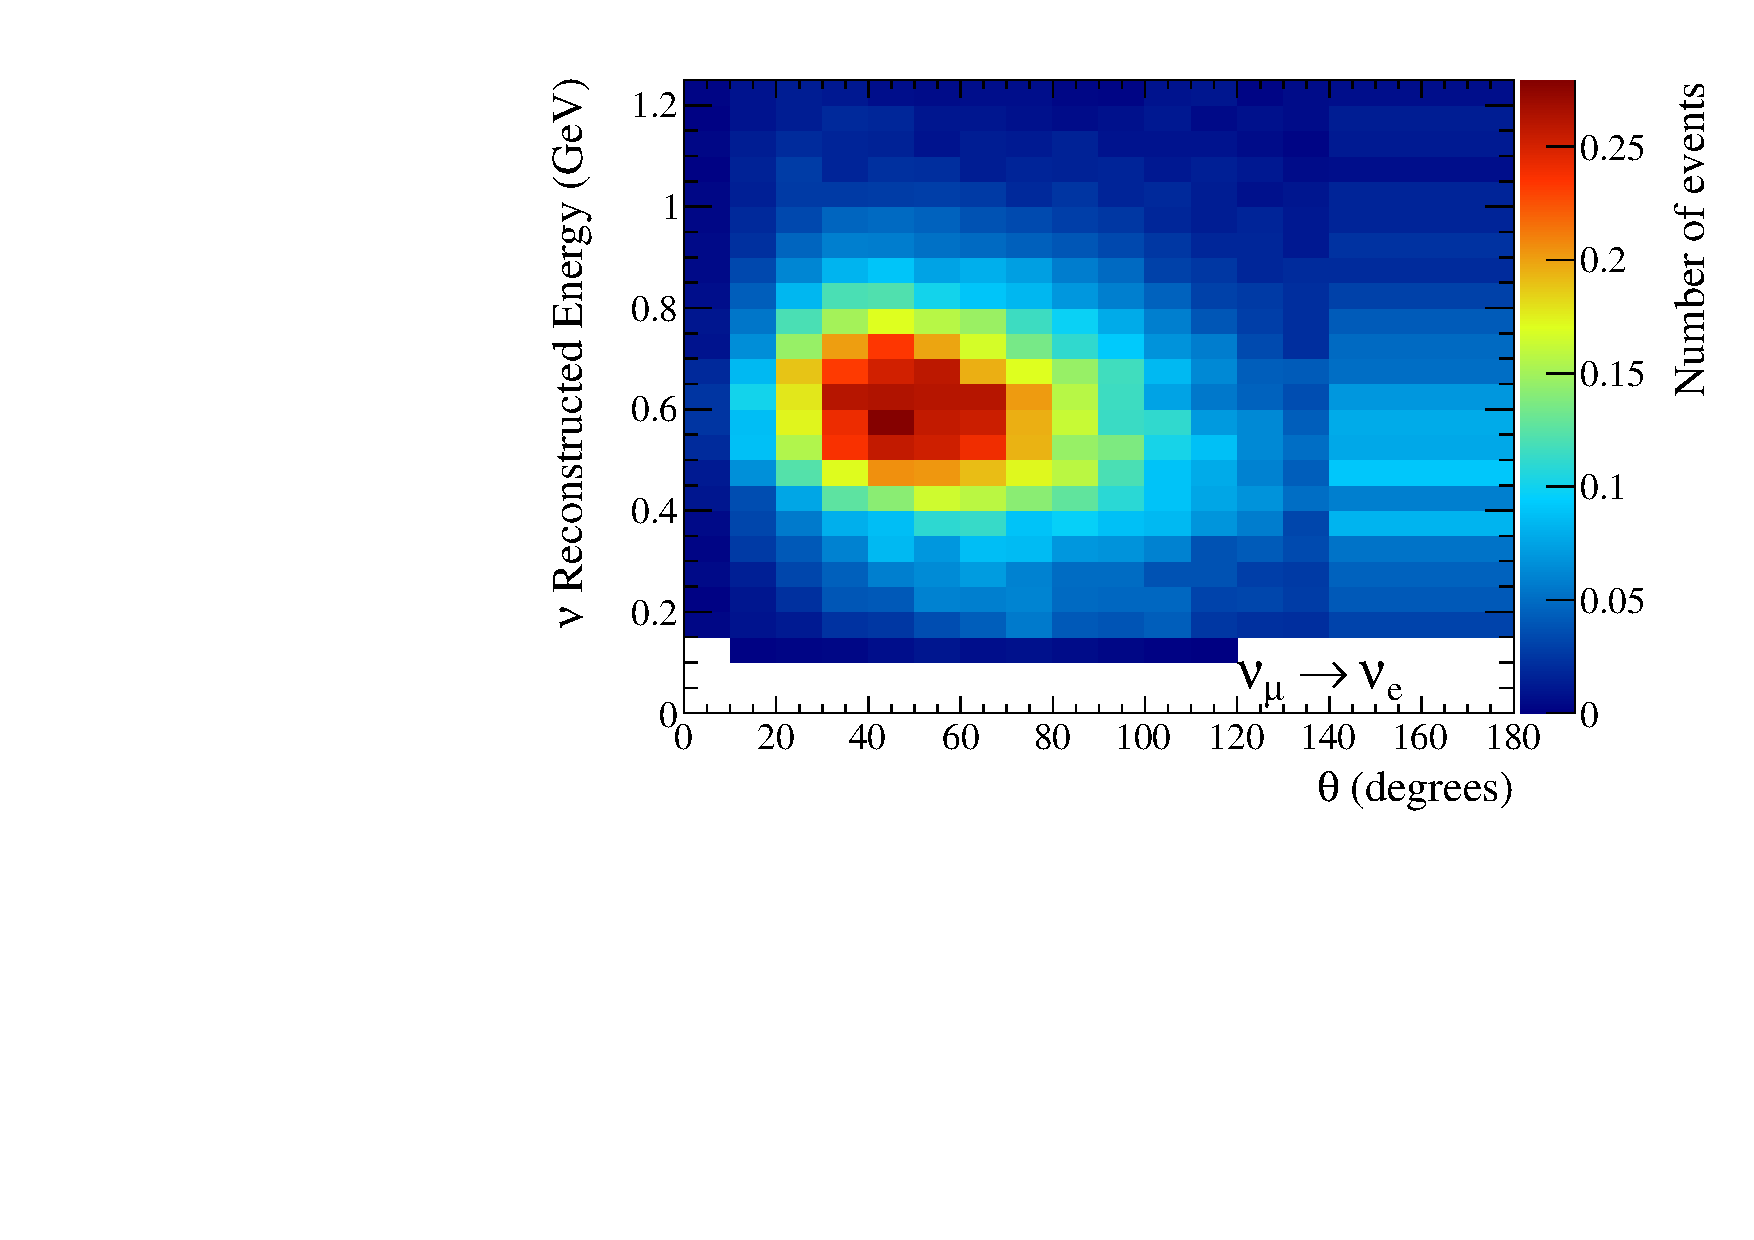
\includegraphics[width=18pc]{joint_plots/spectrum_predictions/template_ereco_vs_theta_numutonue_1re.pdf}
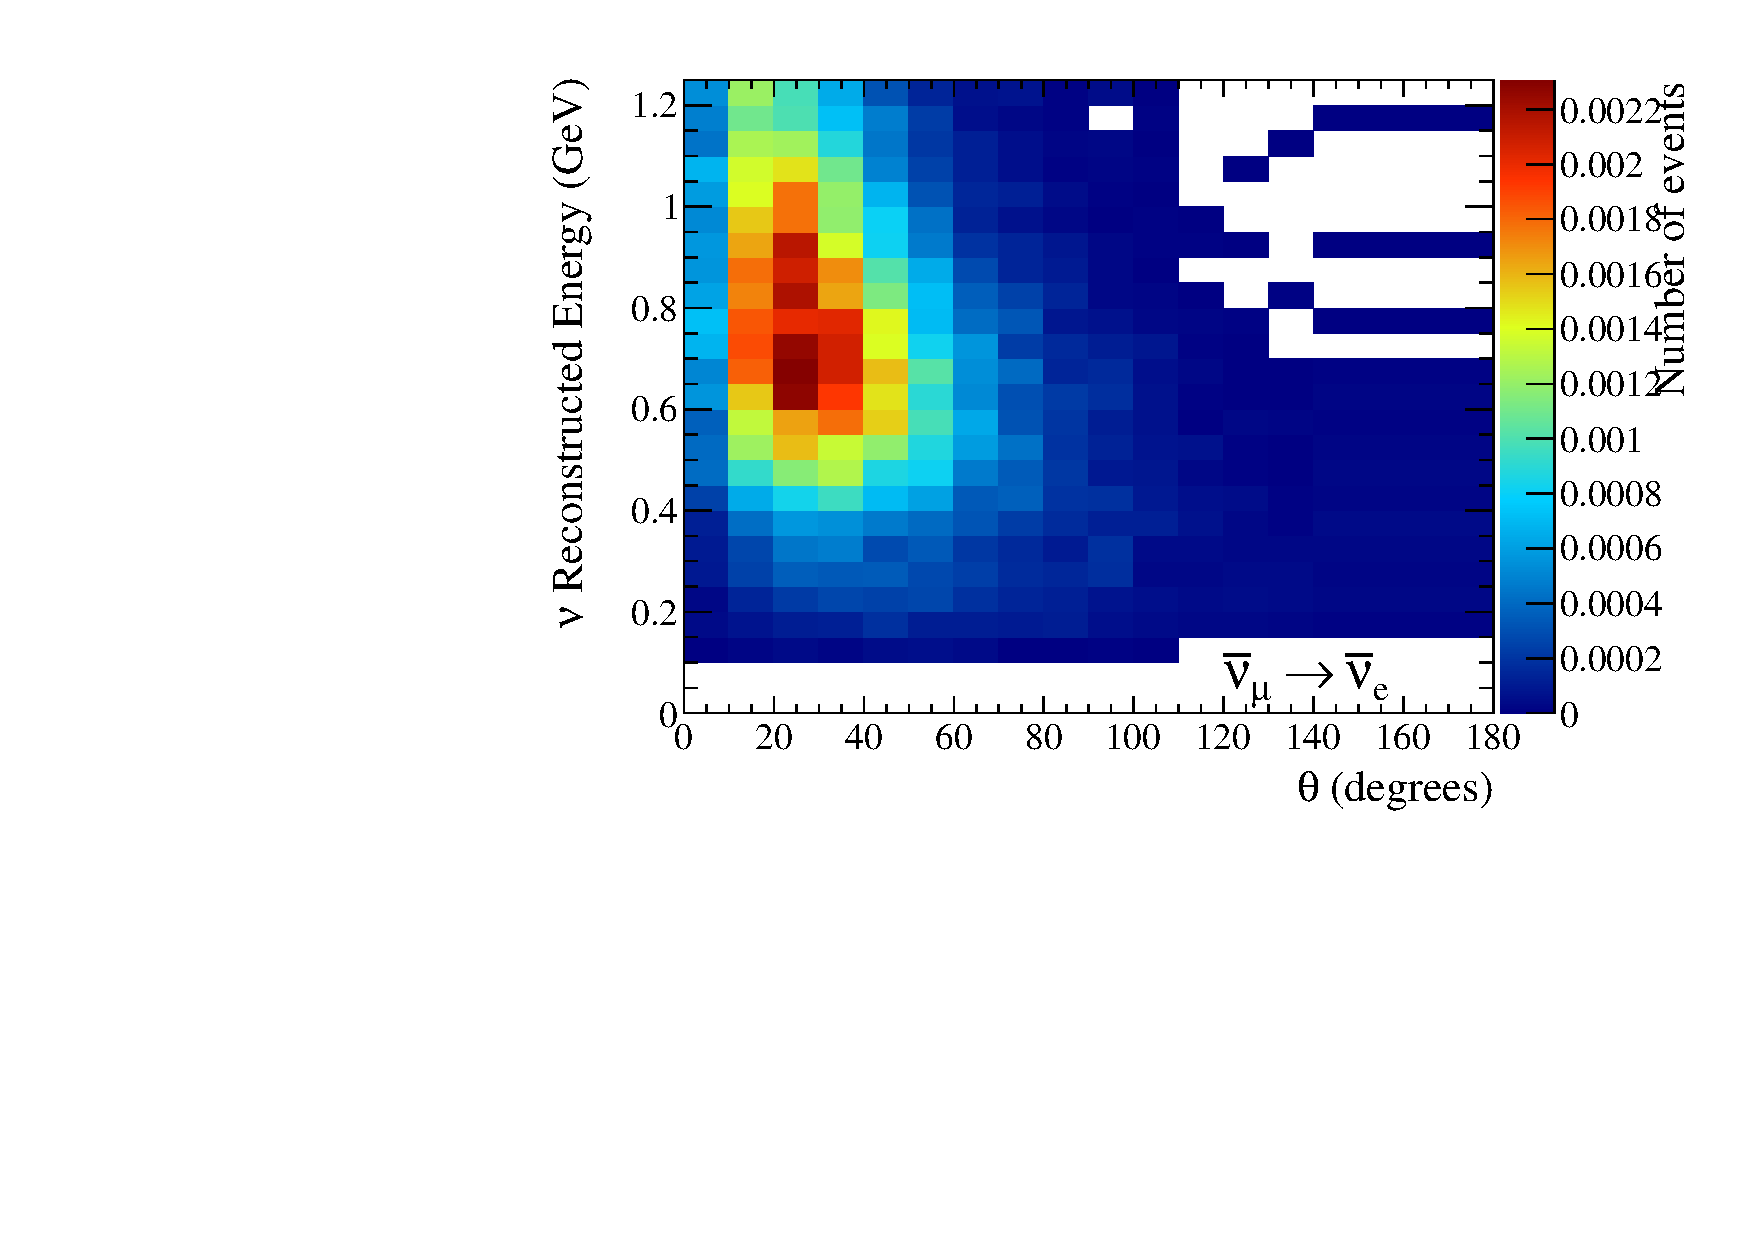
\includegraphics[width=18pc]{joint_plots/spectrum_predictions/template_ereco_vs_theta_numubartonuebar_1re.pdf}
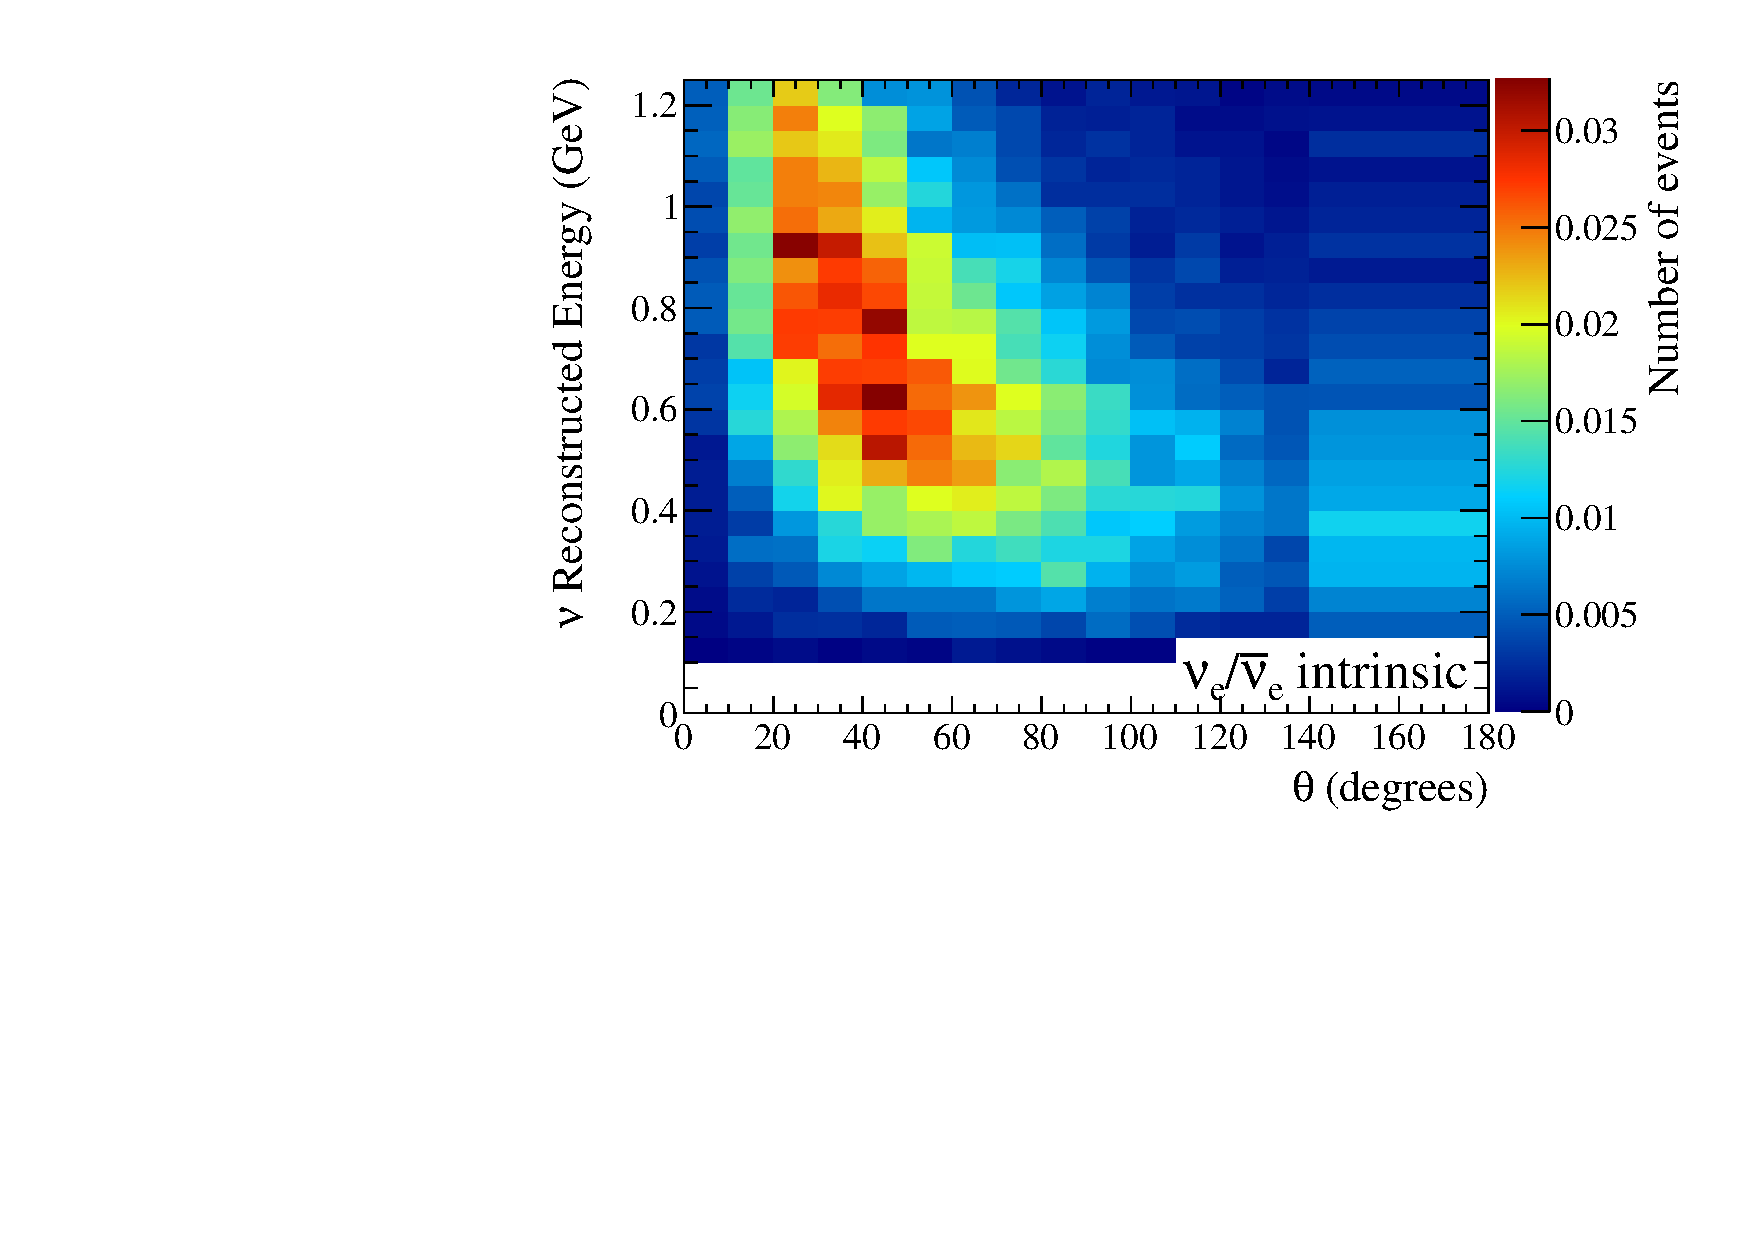
\includegraphics[width=18pc]{joint_plots/spectrum_predictions/template_ereco_vs_theta_nuebeam_1re.pdf}
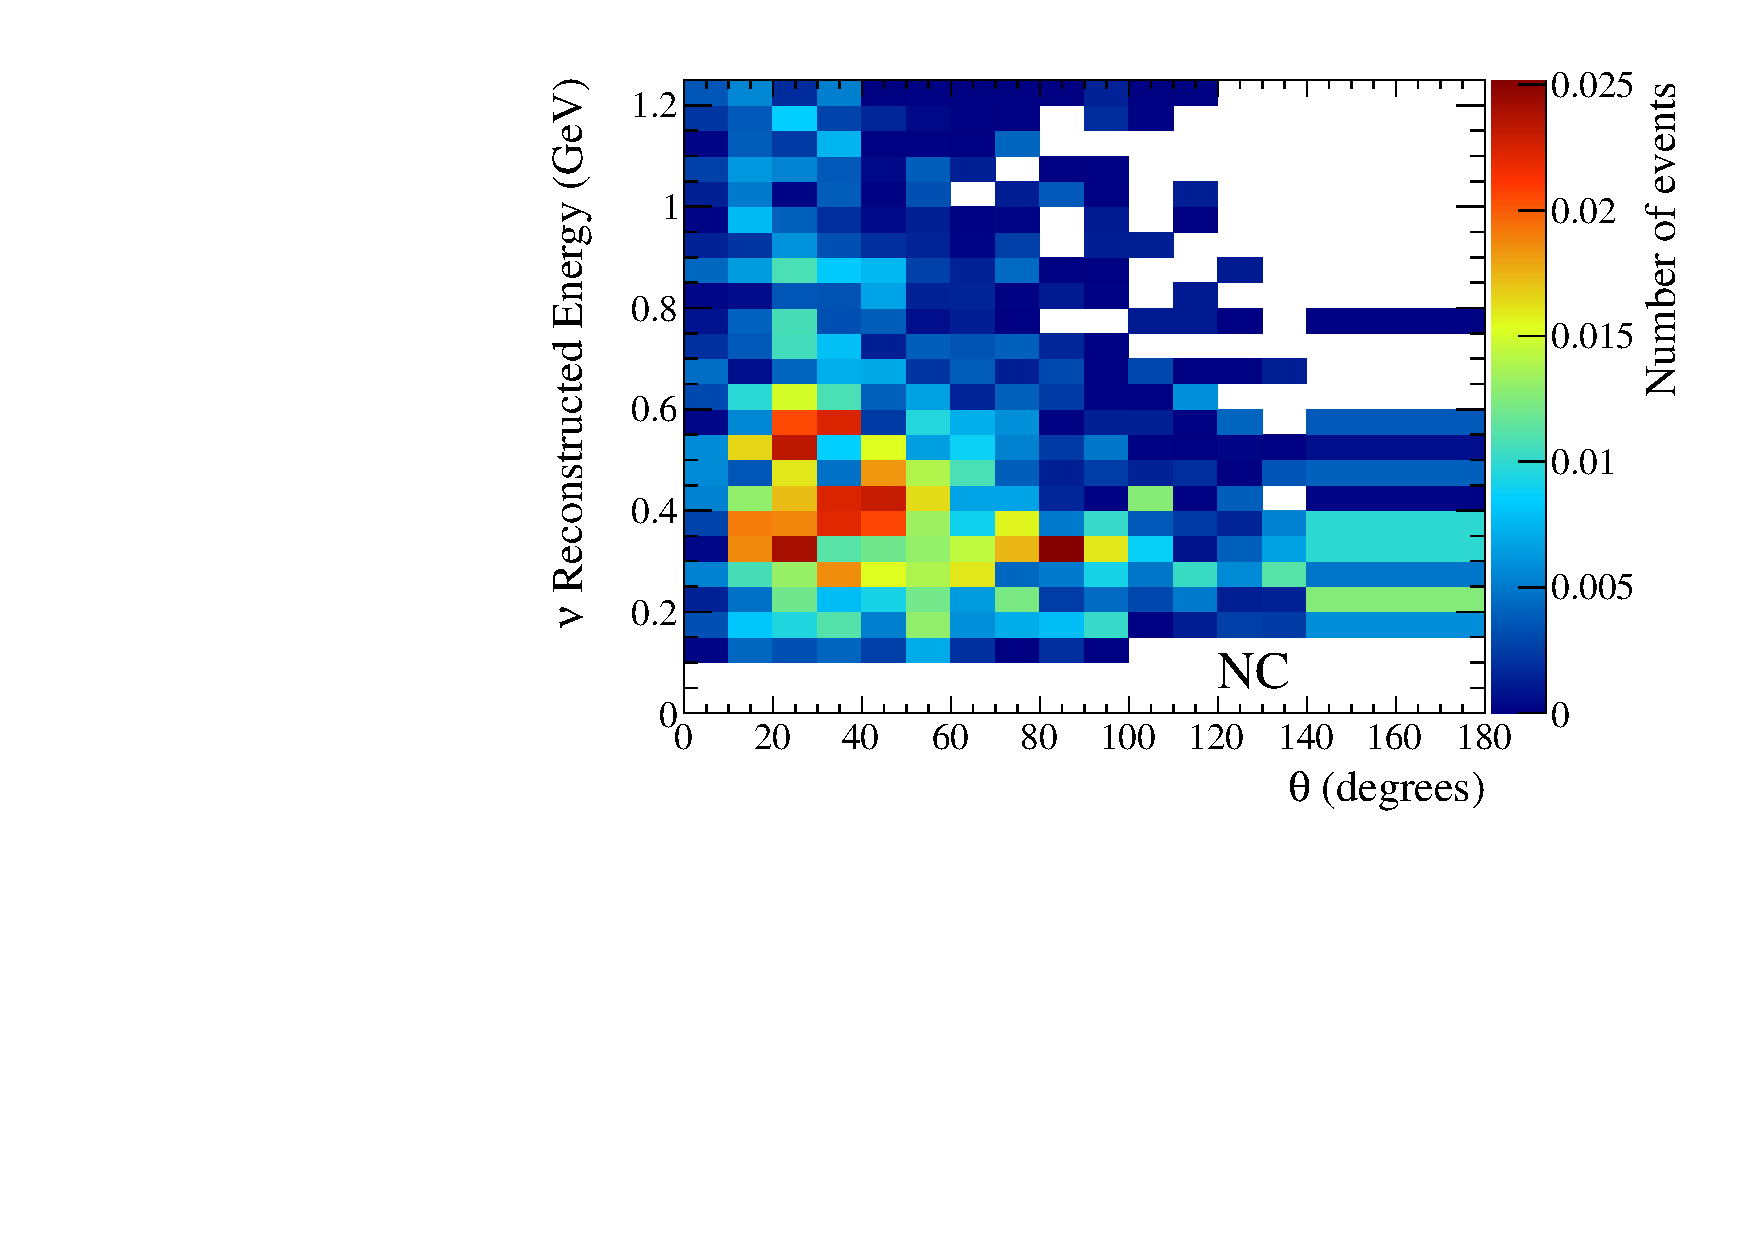
\includegraphics[width=18pc]{joint_plots/spectrum_predictions/template_ereco_vs_theta_nc_1re.pdf}
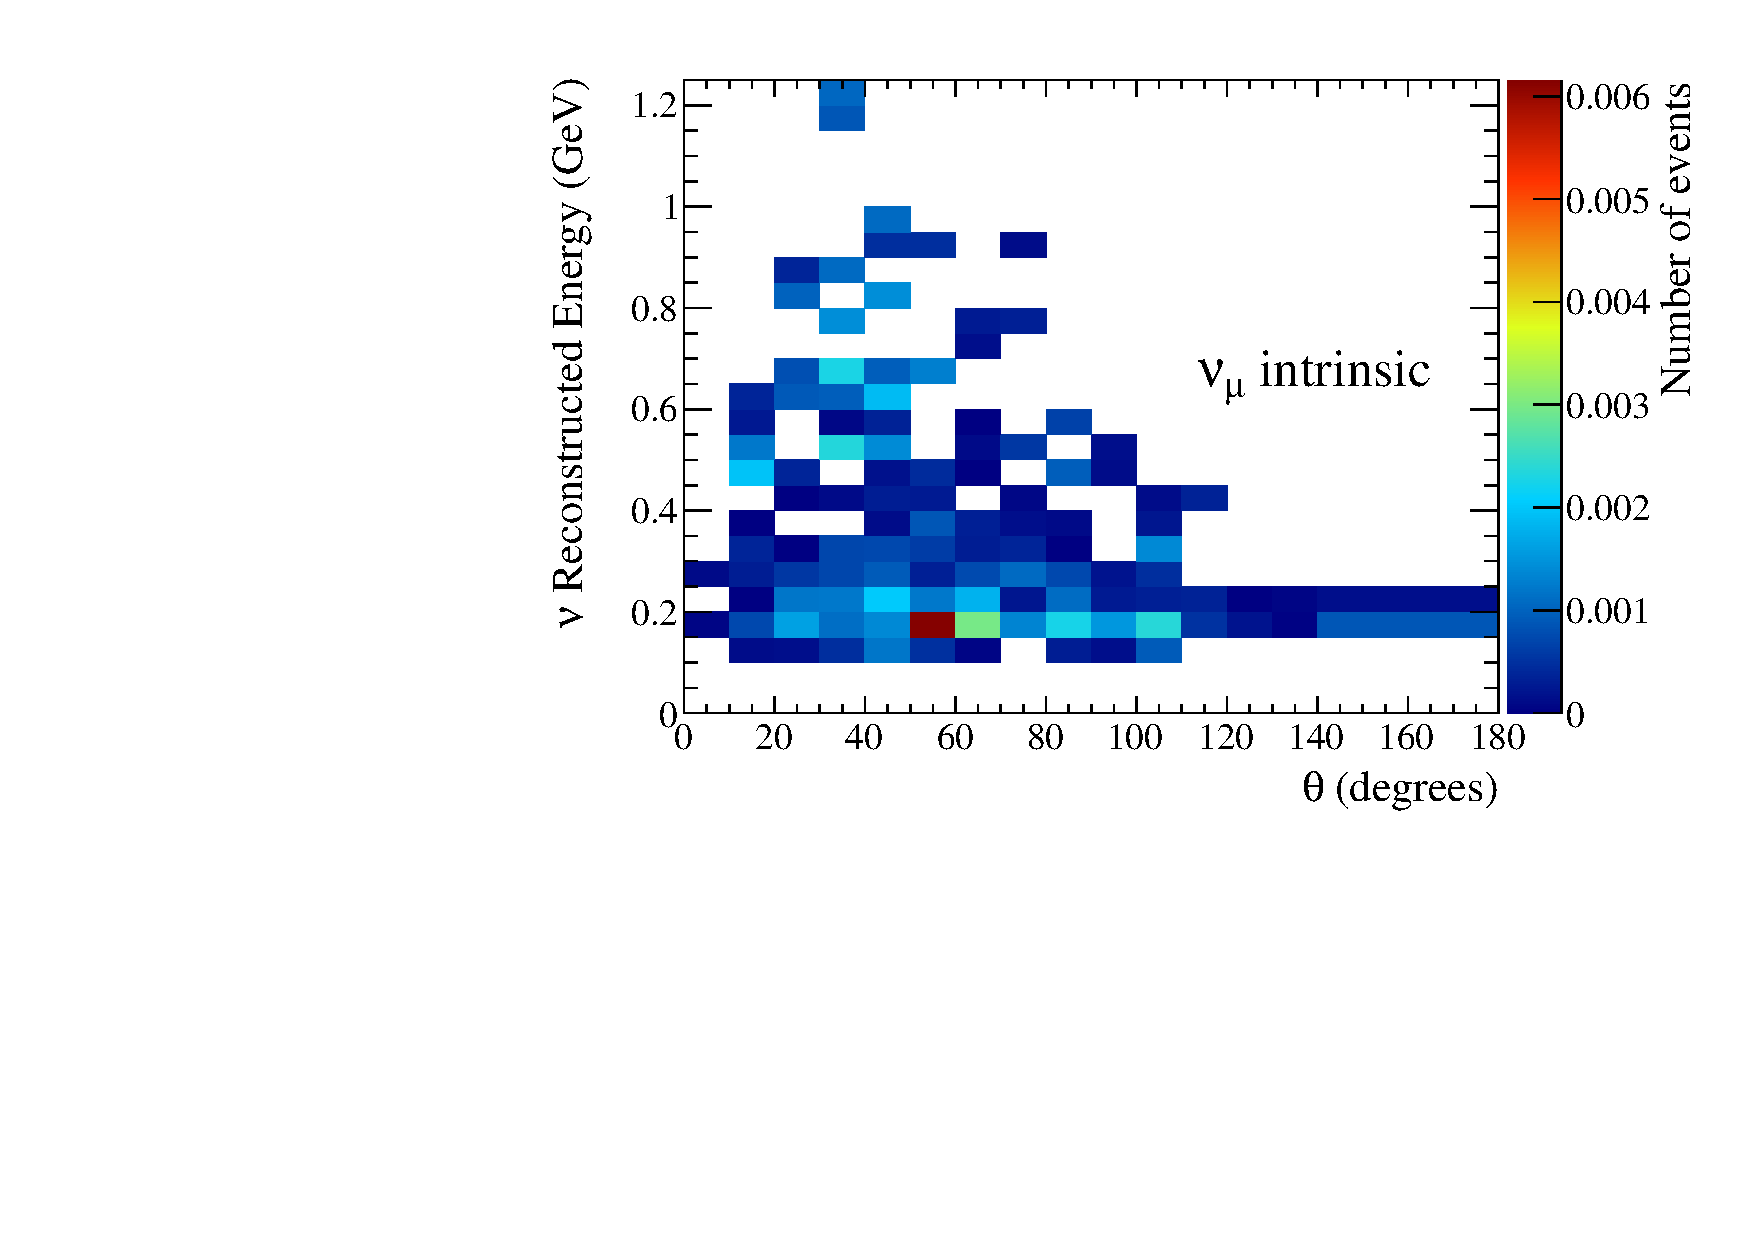
\includegraphics[width=18pc]{joint_plots/spectrum_predictions/template_ereco_vs_theta_numubeam_1re.pdf}
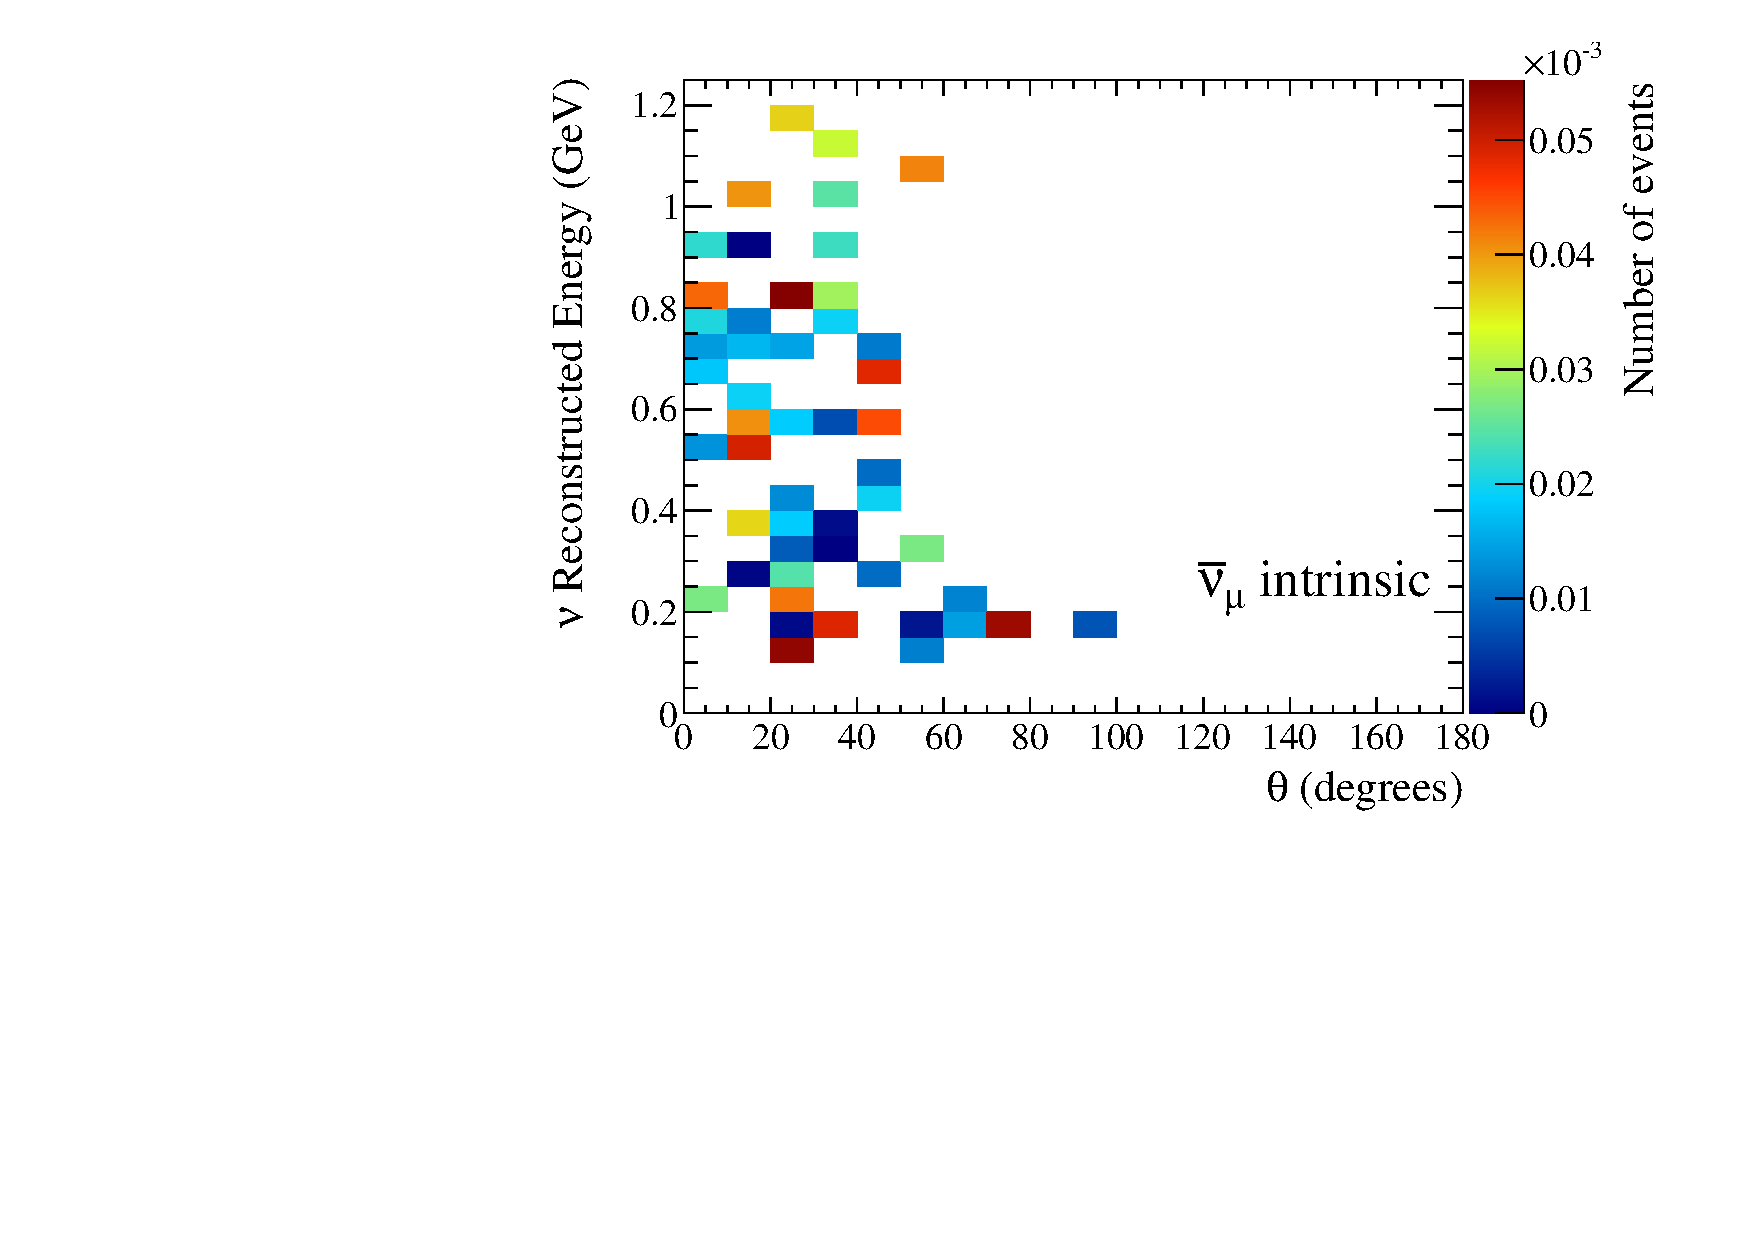
\includegraphics[width=18pc]{joint_plots/spectrum_predictions/template_ereco_vs_theta_numubarbeam_1re.pdf}
\caption {
Predicted spectra of electron-like events
as a function of the reconstructed neutrino energy and
the angle between the outgoing lepton and the neutrino direction.
The distributions correspond to the collected statistics in the full Run 1-6 data set
for an exposure 
of $6.914 \times 10^{20}$ POT in neutrino mode.
%and
%of $4.011 \times 10^{20}$ POT in antineutrino mode.
From top left to bottom right the following components are shown:
total,
$\nu_{\mu} \rightarrow \nu_e$,
$\bar{\nu}_{\mu} \rightarrow \bar{\nu}_e$,
$\nu_e + \bar{\nu}_e$ intrinsic beam,
NC,
$\nu_{\mu}$ intrinsic beam
and
$\bar{\nu}_{\mu}$ intrinsic beam.
The spectra were generated with the systematic parameters measured with the ND280 data 
shown in tab.~\ref{tab:banff_uncertainties_flux_fhc},~\ref{tab:banff_uncertainties_flux_rhc},~\ref{tab:banff_uncertainties_xsec}
and \ref{tab:banff_uncertainties_skdetfsi}
and the oscillation parameters corresponding to the Asimov data set A shown in tab.~\ref{tab:osc_params_joint_asimov}.
}
\label{fig:joint_ereco_vs_theta_1re}
\end{figure*}

\begin{figure*}[htb]
%\hspace{0.06\linewidth}
\center
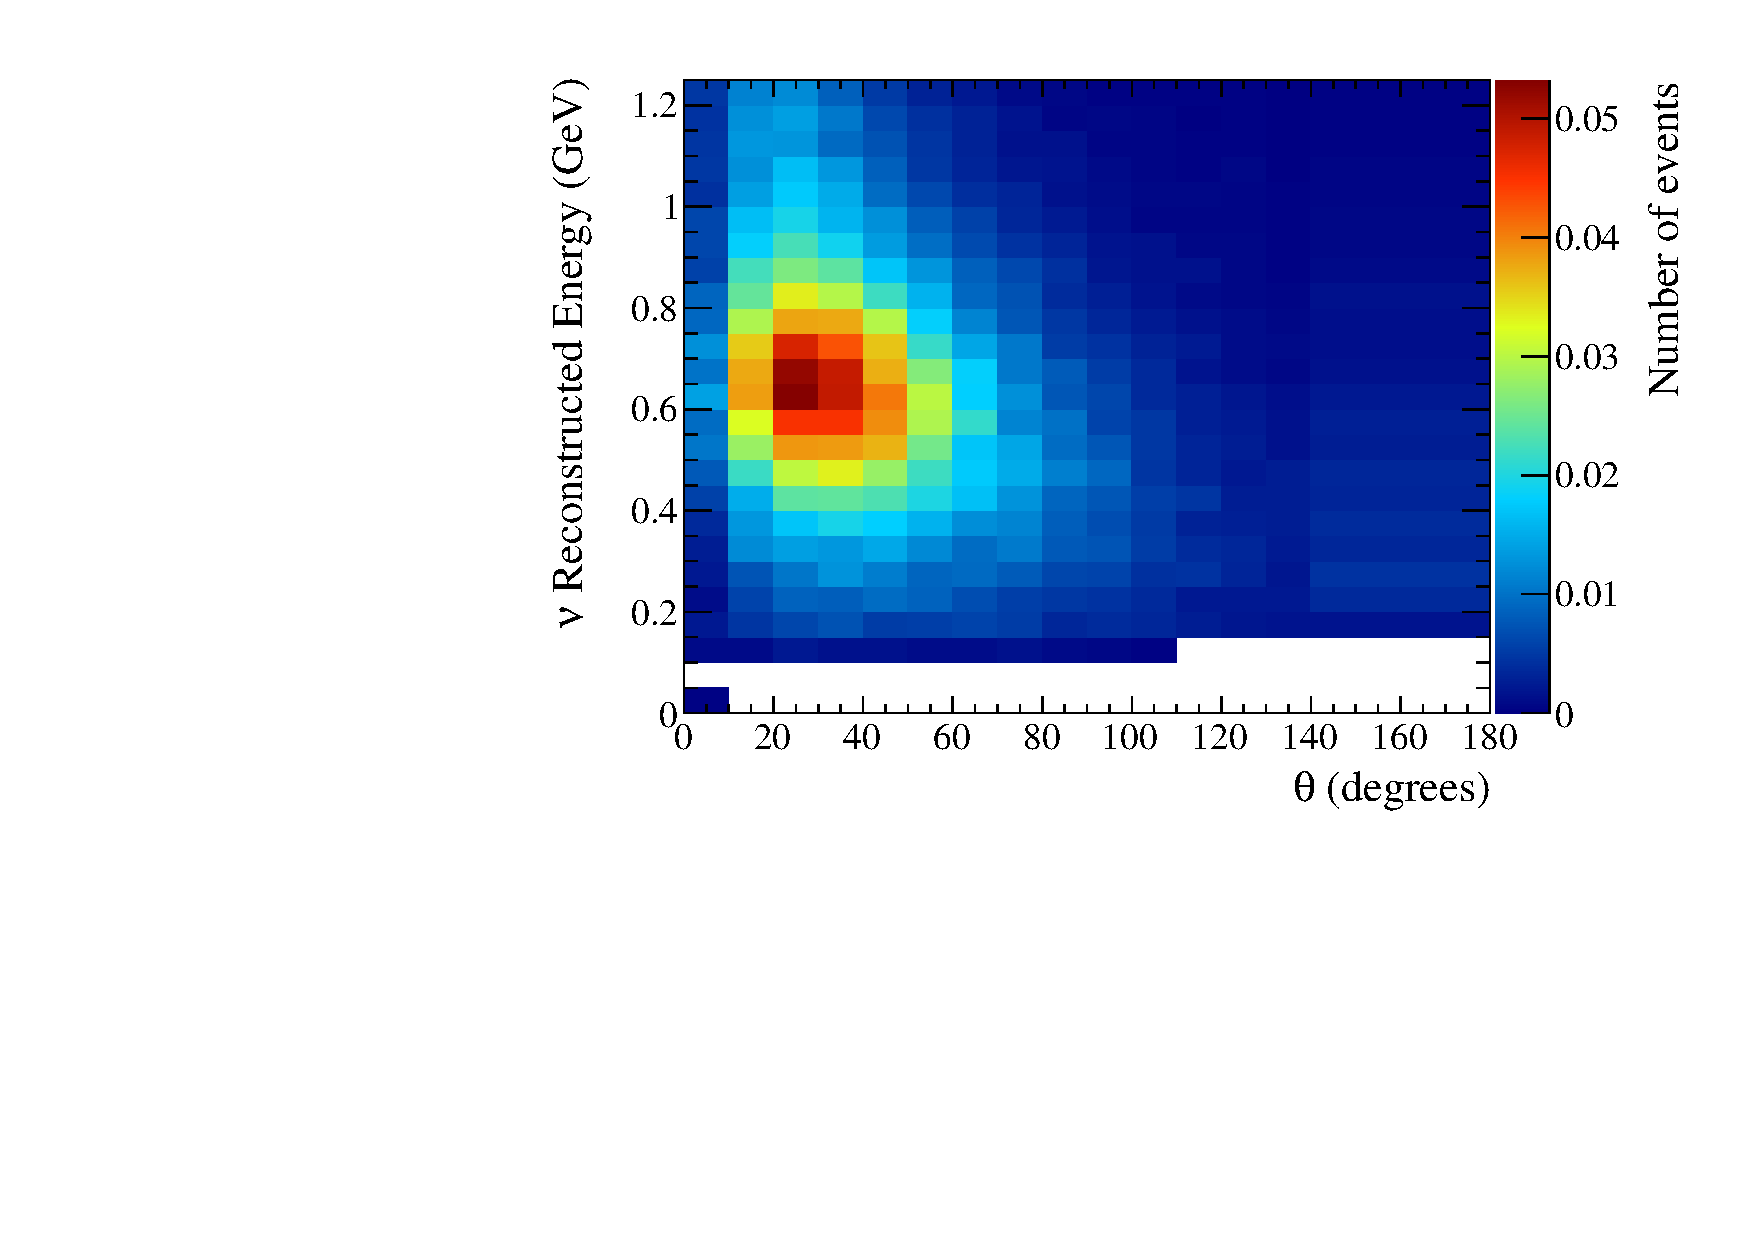
\includegraphics[width=18pc]{joint_plots/spectrum_predictions/template_ereco_vs_theta_tot_rhc1re.pdf}\\
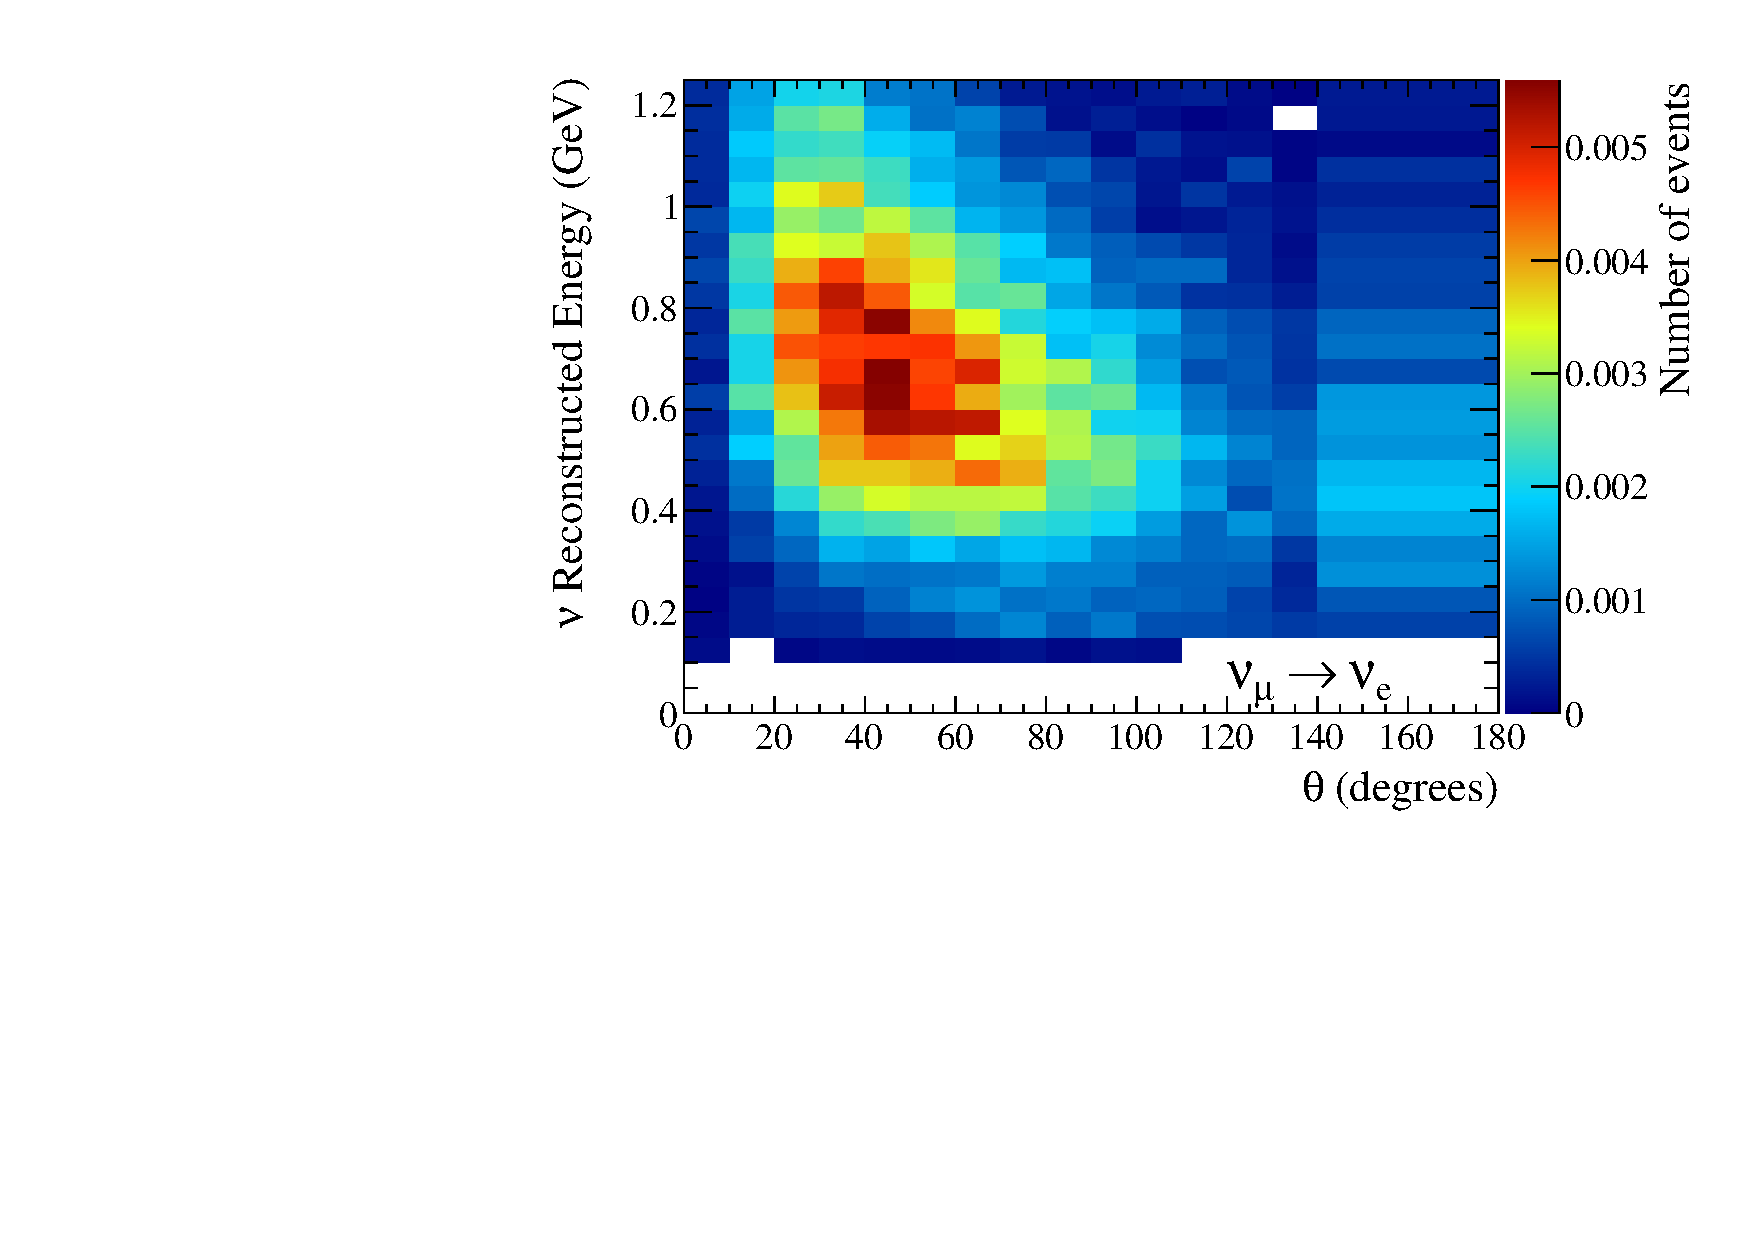
\includegraphics[width=18pc]{joint_plots/spectrum_predictions/template_ereco_vs_theta_numutonue_rhc1re.pdf}
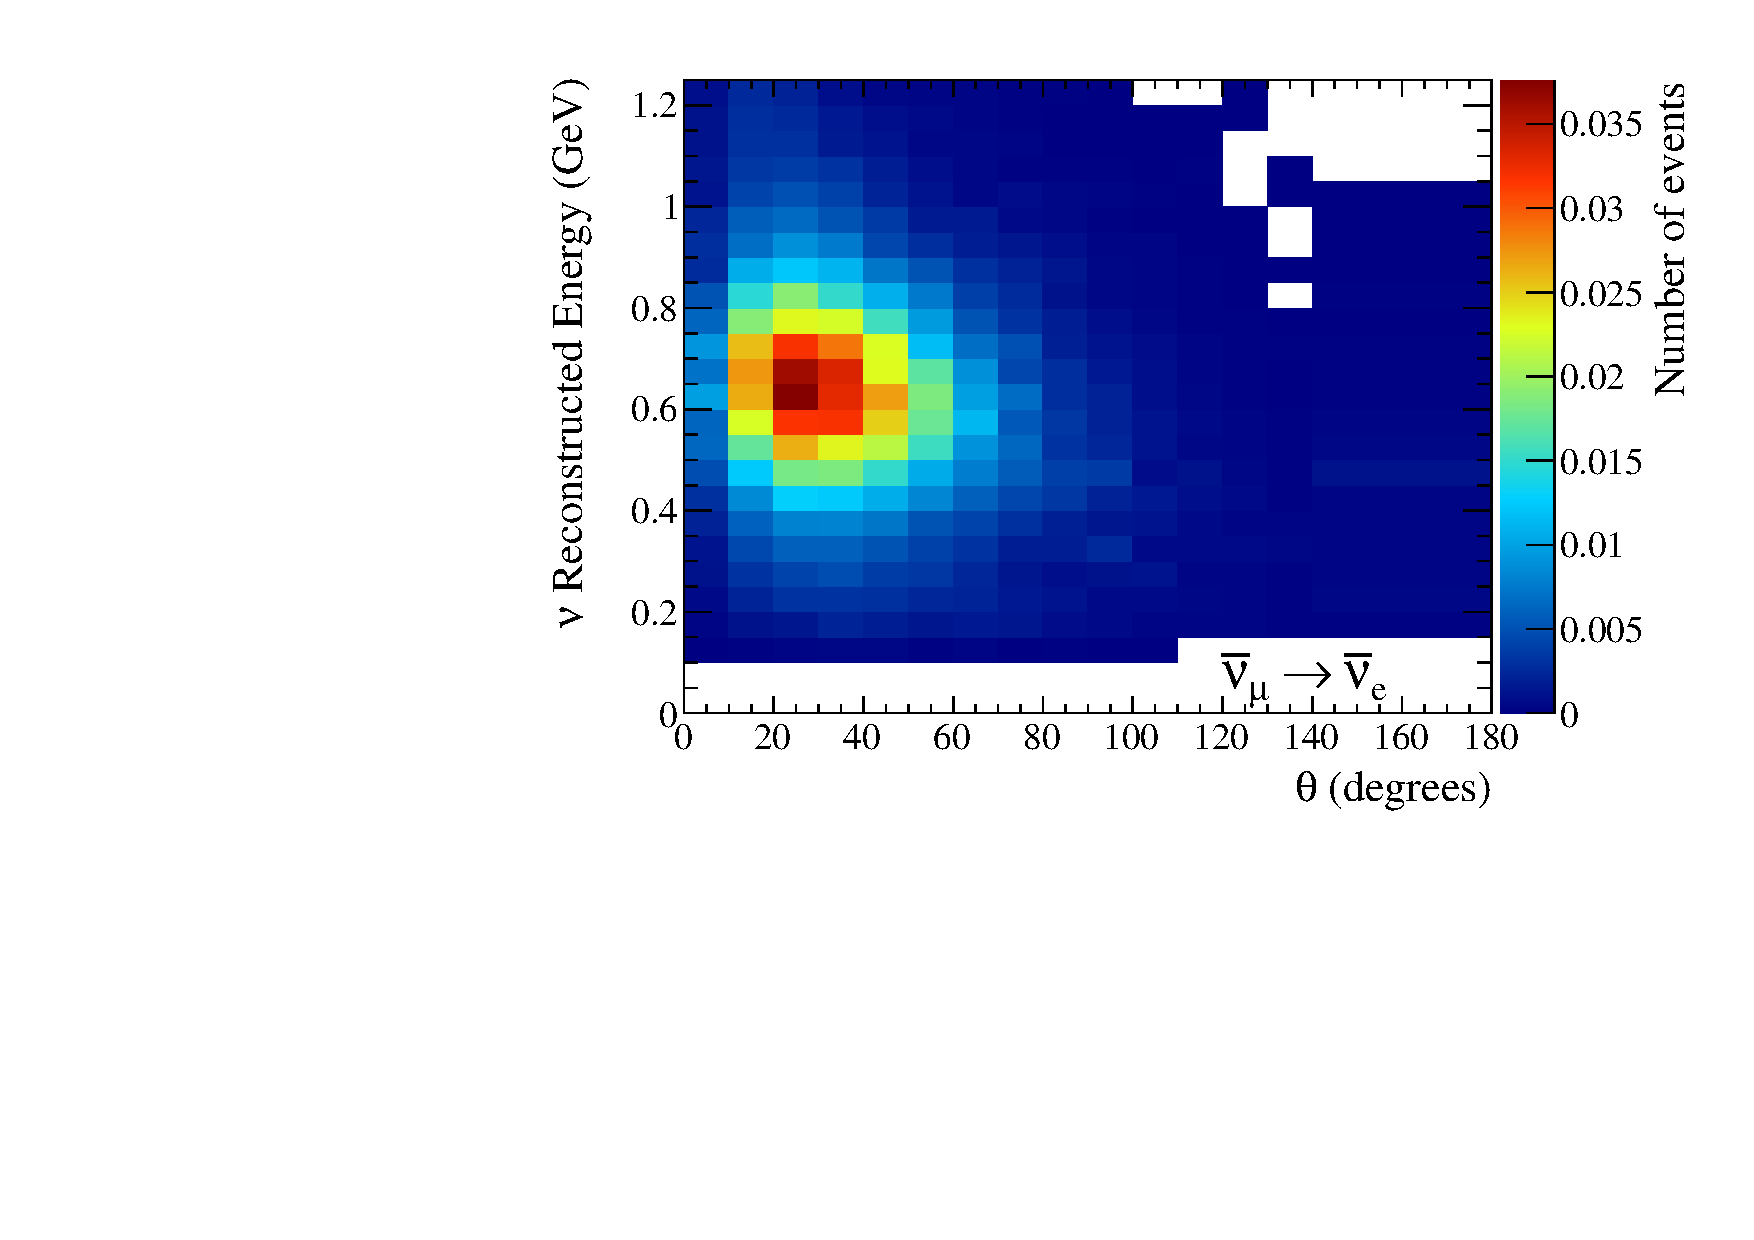
\includegraphics[width=18pc]{joint_plots/spectrum_predictions/template_ereco_vs_theta_numubartonuebar_rhc1re.pdf}
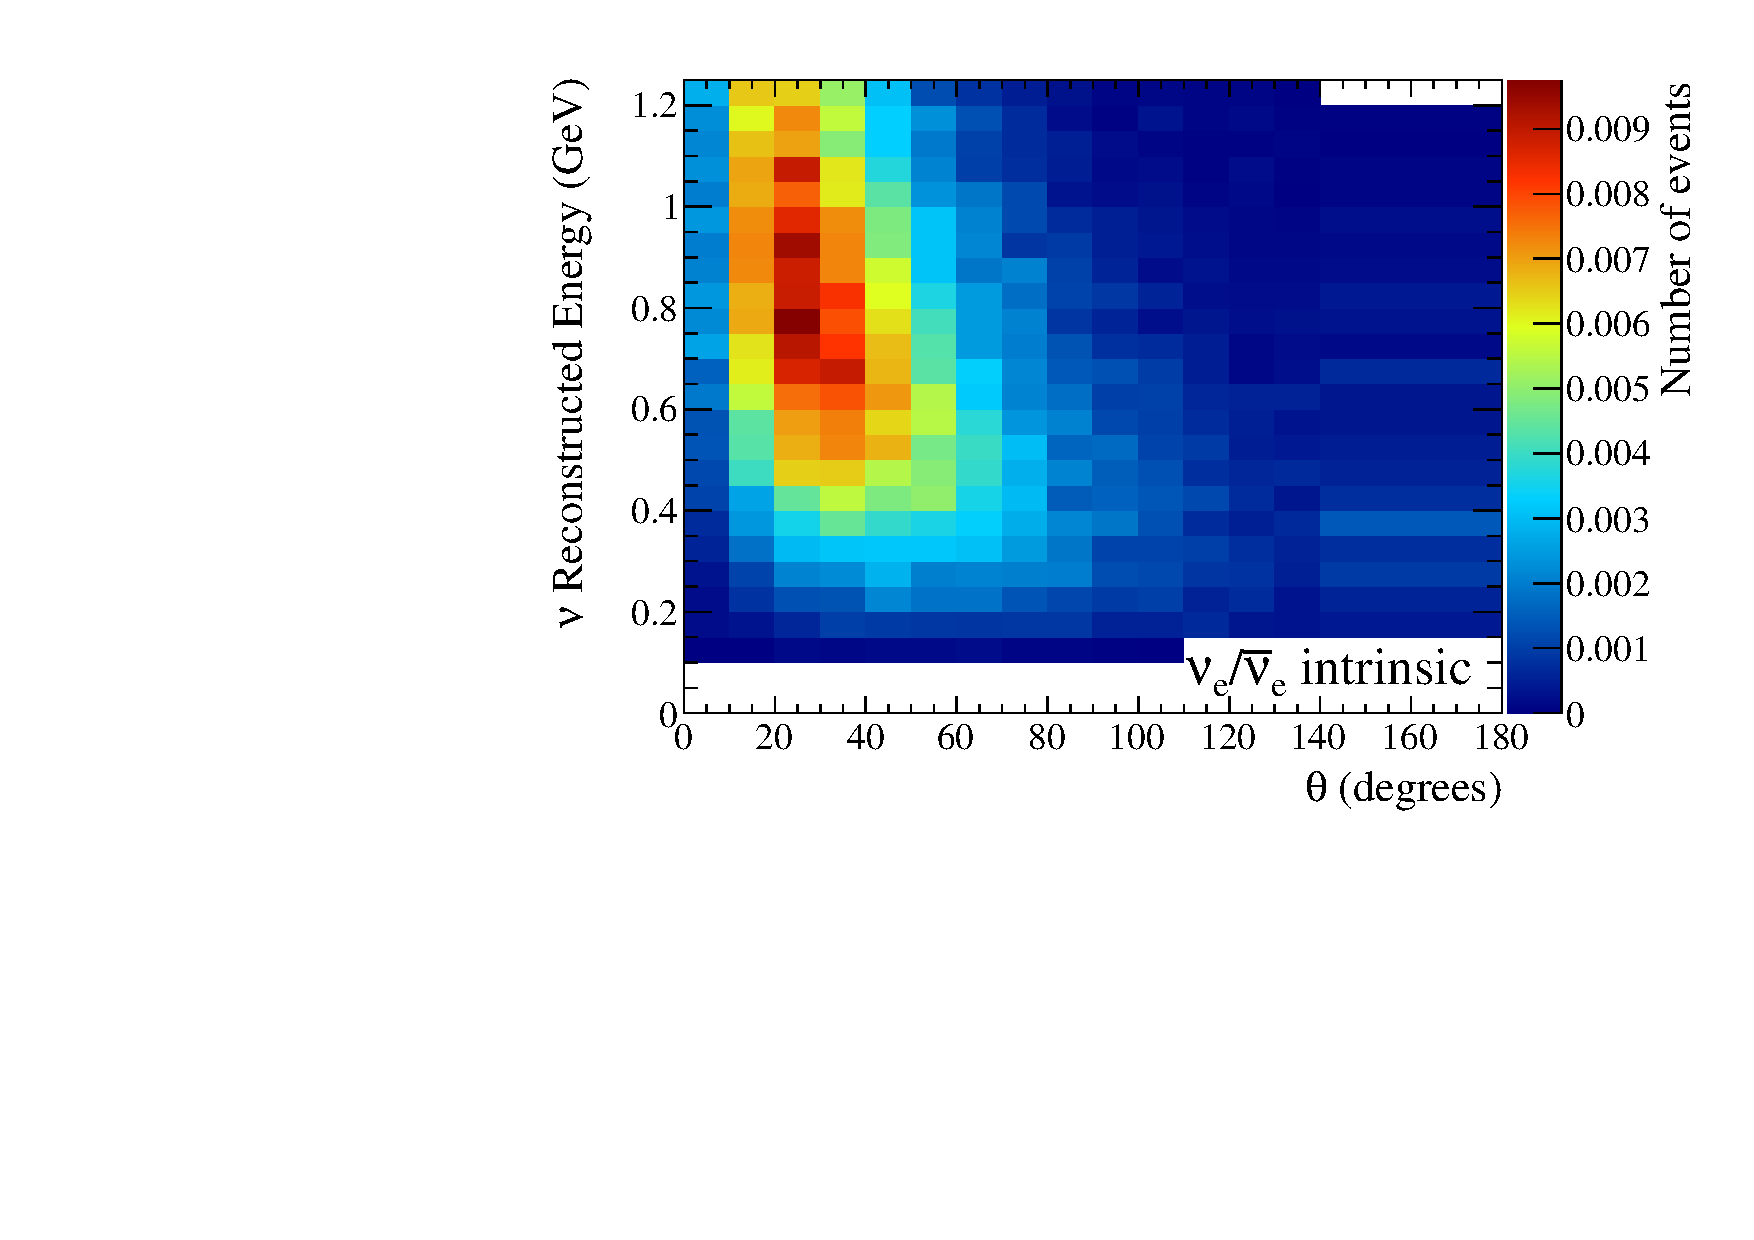
\includegraphics[width=18pc]{joint_plots/spectrum_predictions/template_ereco_vs_theta_nuebeam_rhc1re.pdf}
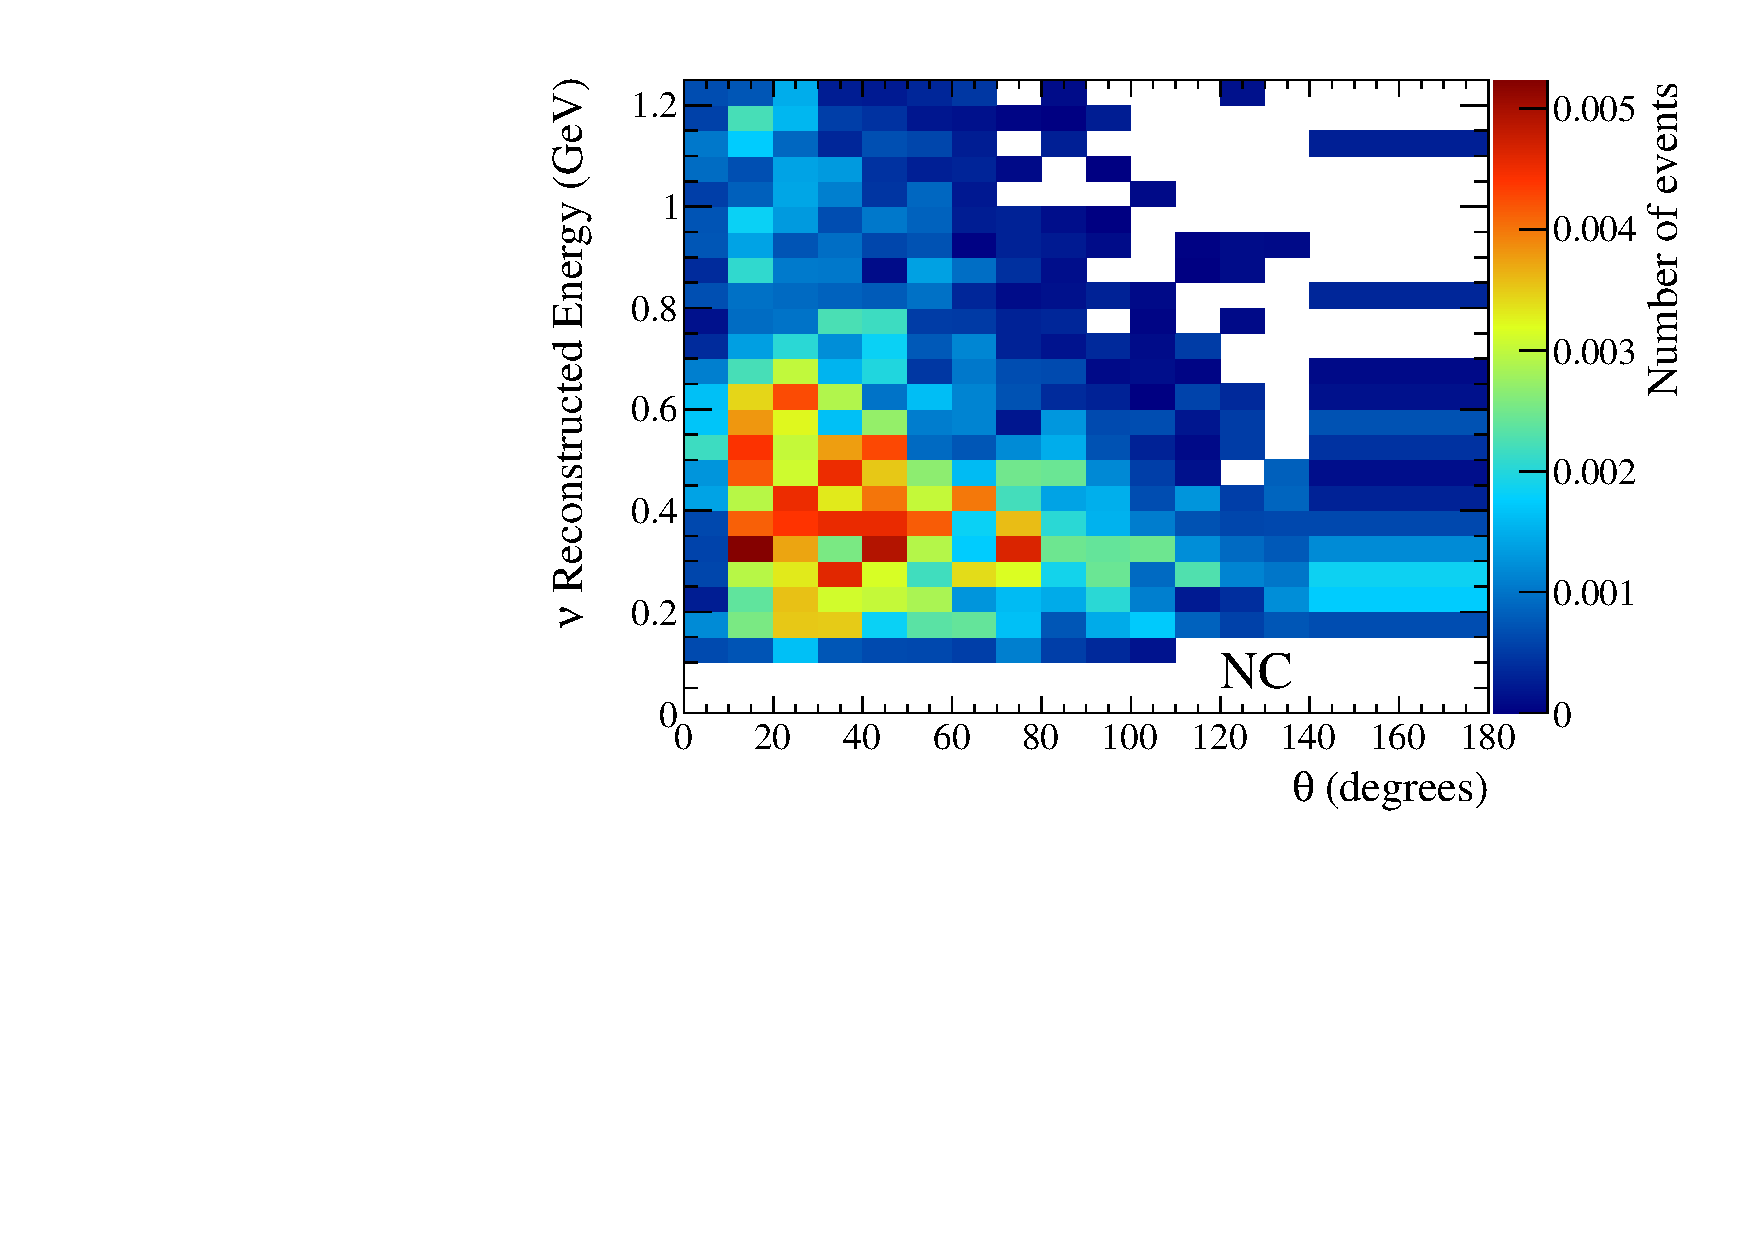
\includegraphics[width=18pc]{joint_plots/spectrum_predictions/template_ereco_vs_theta_nc_rhc1re.pdf}
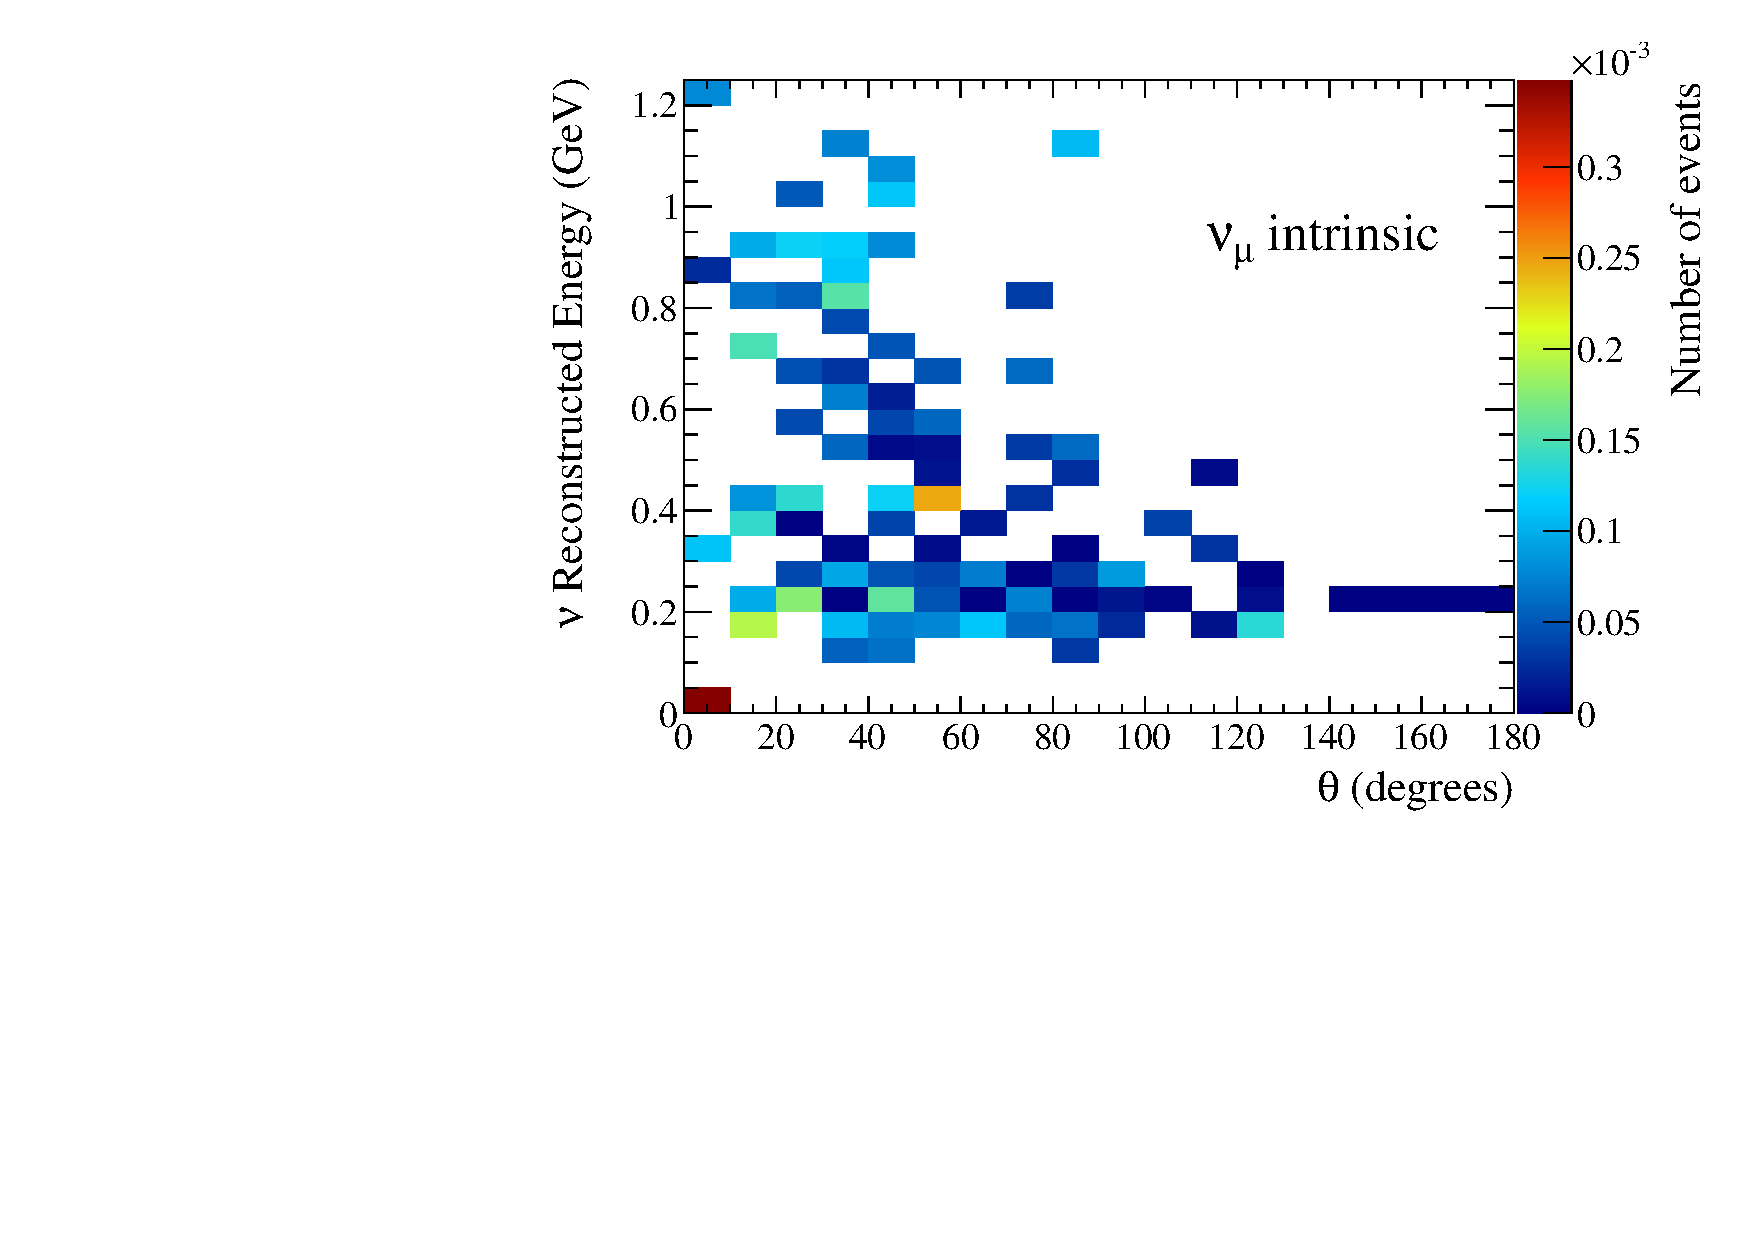
\includegraphics[width=18pc]{joint_plots/spectrum_predictions/template_ereco_vs_theta_numubeam_rhc1re.pdf}
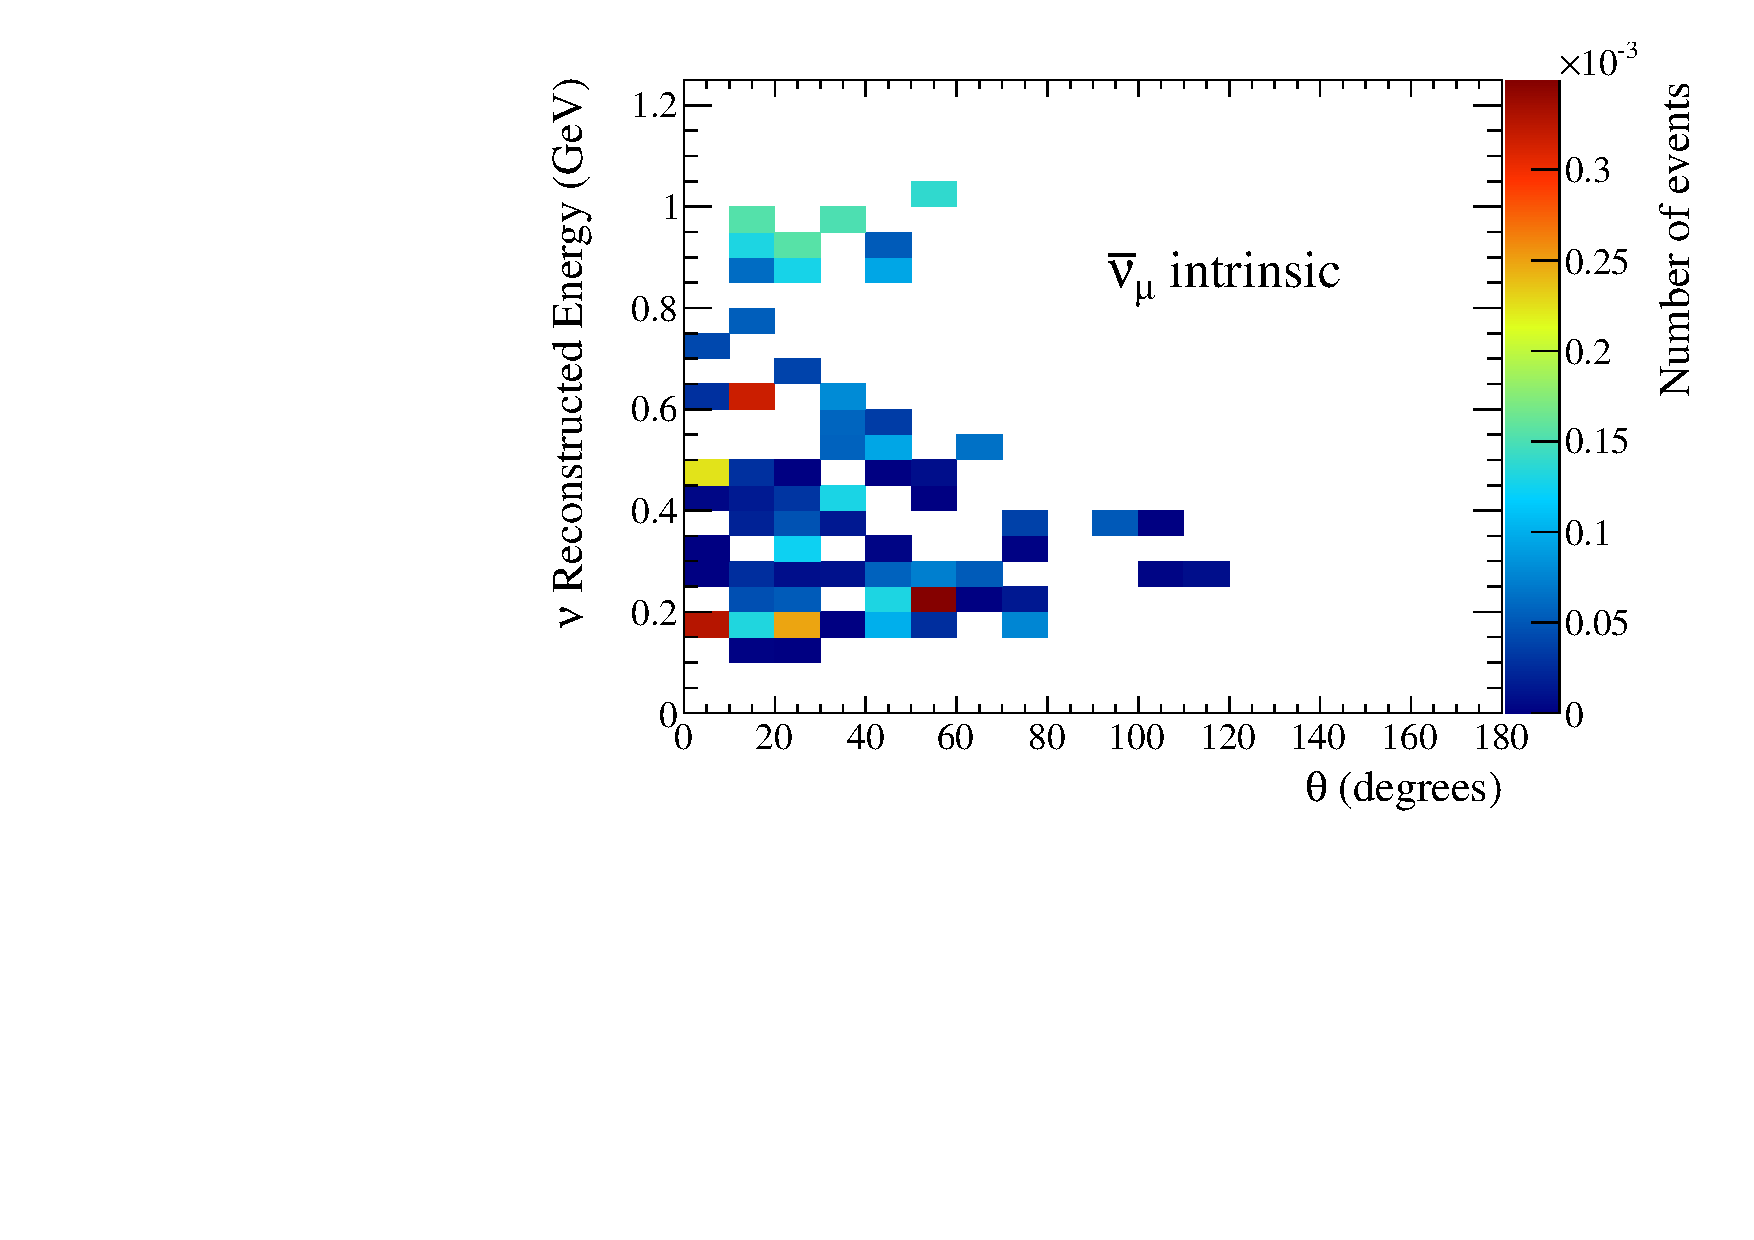
\includegraphics[width=18pc]{joint_plots/spectrum_predictions/template_ereco_vs_theta_numubarbeam_rhc1re.pdf}
%\includegraphics[width=42pc]{../plots/plot_sk_osc/jointfit_plots/spectra_data/rhc1re_components.pdf}
\caption {
Predicted spectra of electron-like events
as a function of the reconstructed neutrino energy and
the angle between the outgoing lepton and the neutrino direction.
The distributions correspond to the collected statistics in the full Run 1-6 data set
for an exposure 
%of $6.914 \times 10^{20}$ POT in neutrino  mode.
%and
of $4.011 \times 10^{20}$ POT in antineutrino mode.
From top left to bottom right the following components are shown:
total,
$\nu_{\mu} \rightarrow \nu_e$,
$\bar{\nu}_{\mu} \rightarrow \bar{\nu}_e$,
$\nu_e + \bar{\nu}_e$ intrinsic beam,
NC,
$\nu_{\mu}$ intrinsic beam
and
$\bar{\nu}_{\mu}$ intrinsic beam.
The spectra were generated with the systematic parameters measured with the ND280 data 
shown in tab.~\ref{tab:banff_uncertainties_flux_fhc},~\ref{tab:banff_uncertainties_flux_rhc},~\ref{tab:banff_uncertainties_xsec}
and \ref{tab:banff_uncertainties_skdetfsi}
and the oscillation parameters corresponding to the Asimov data set A shown in tab.~\ref{tab:osc_params_joint_asimov}.
}
\label{fig:joint_ereco_vs_theta_rhc1re}
\end{figure*}


In Fig.~\ref{fig:joint_1d_elike} the projection of the 2-dimensional $e$-like templates
onto the $E_{reco}$ and $\theta$ axes are shown.

\begin{figure*}[htb]
%\hspace{0.06\linewidth}
\center
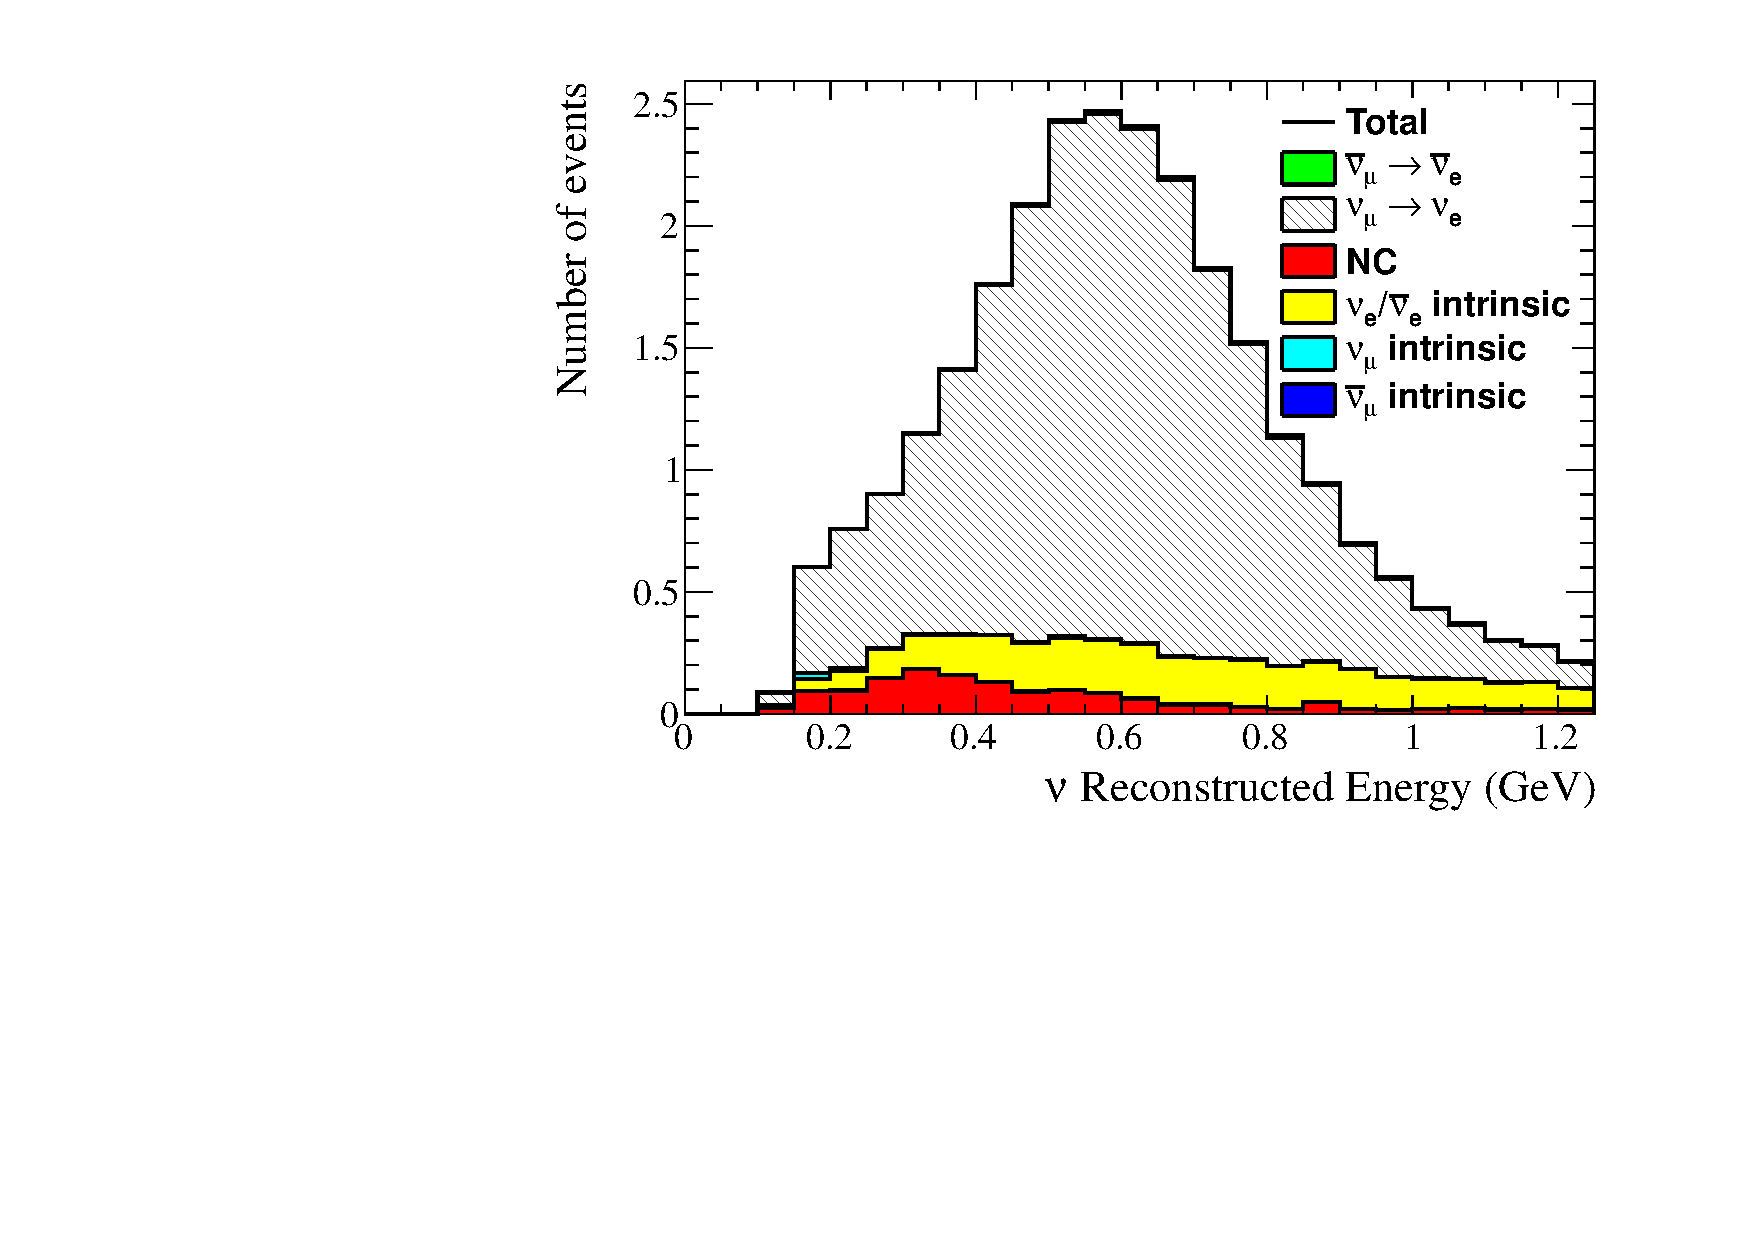
\includegraphics[width=18pc]{joint_plots/spectrum_predictions/template_ereco_1re.pdf}
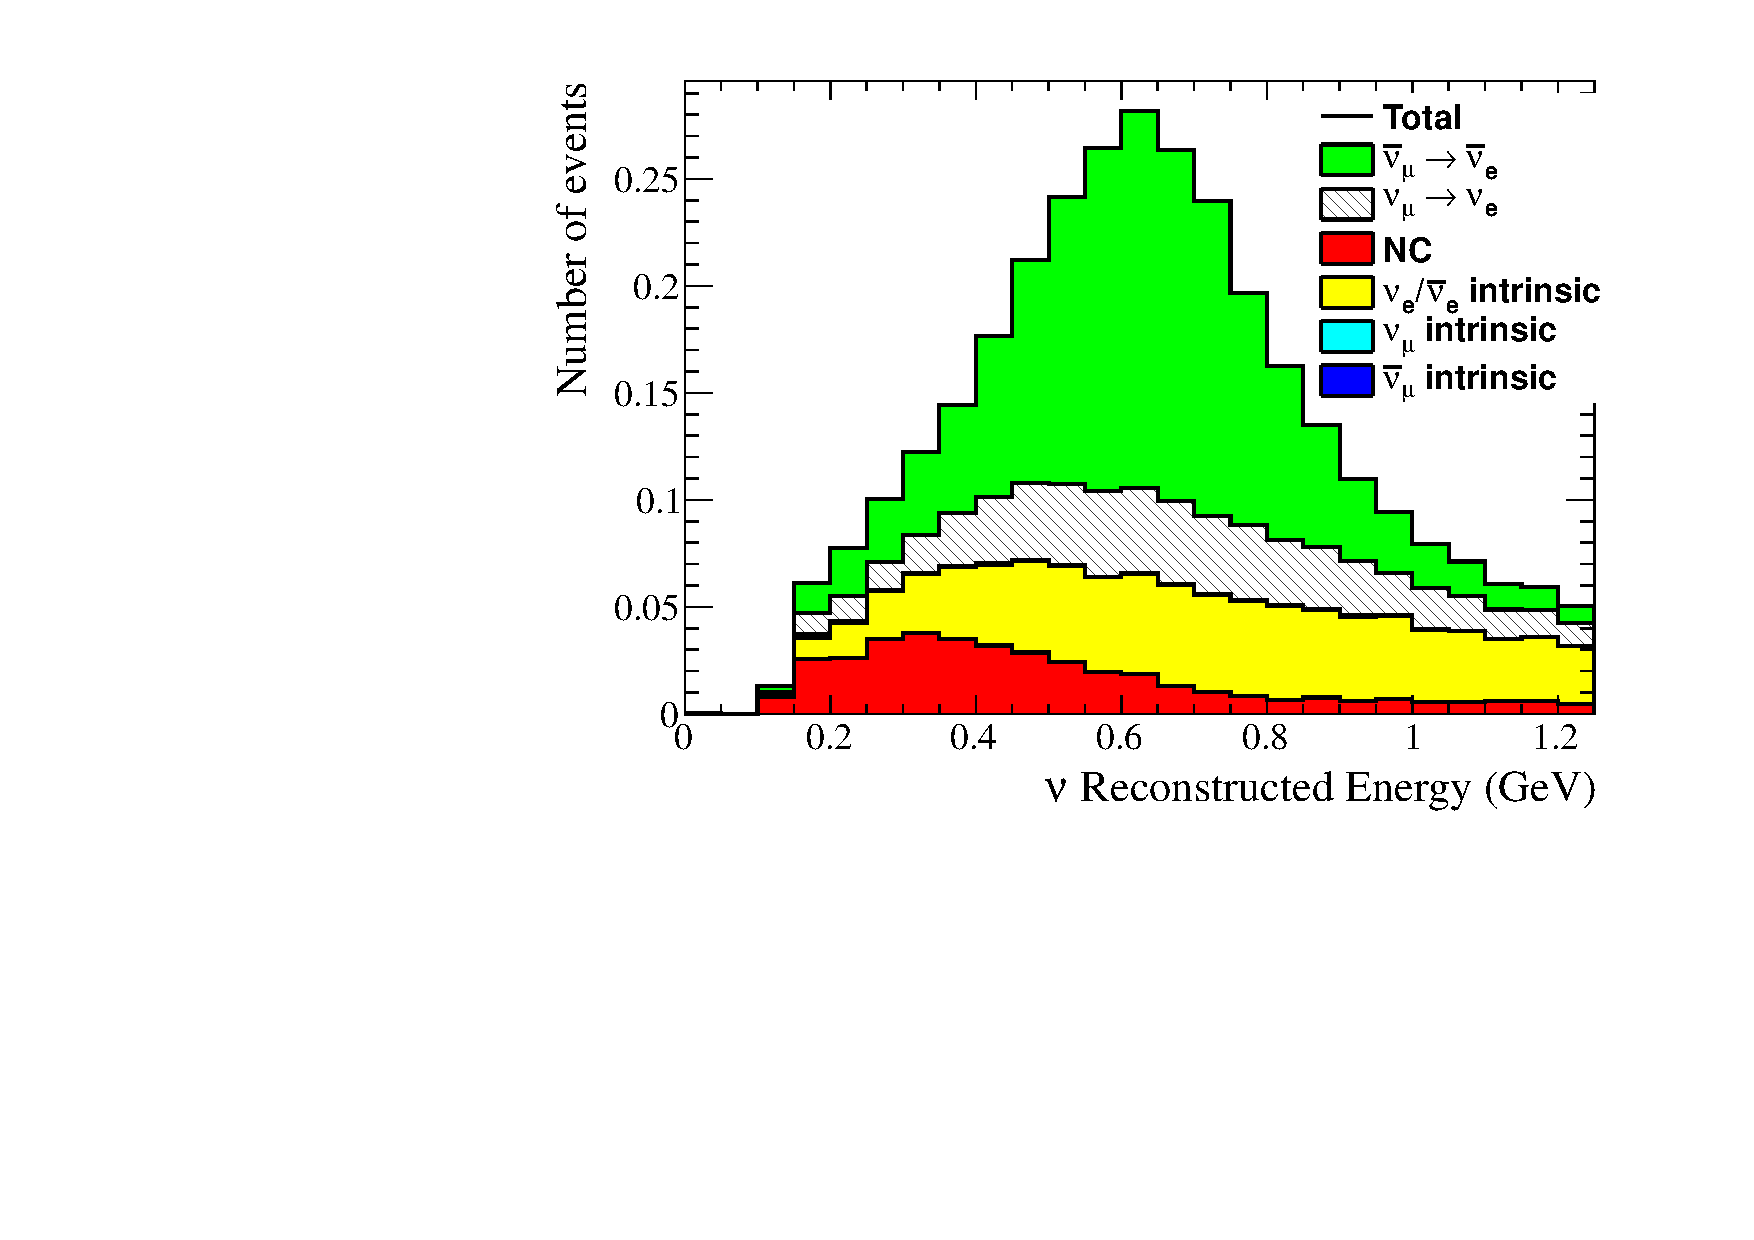
\includegraphics[width=18pc]{joint_plots/spectrum_predictions/template_ereco_rhc1re.pdf}
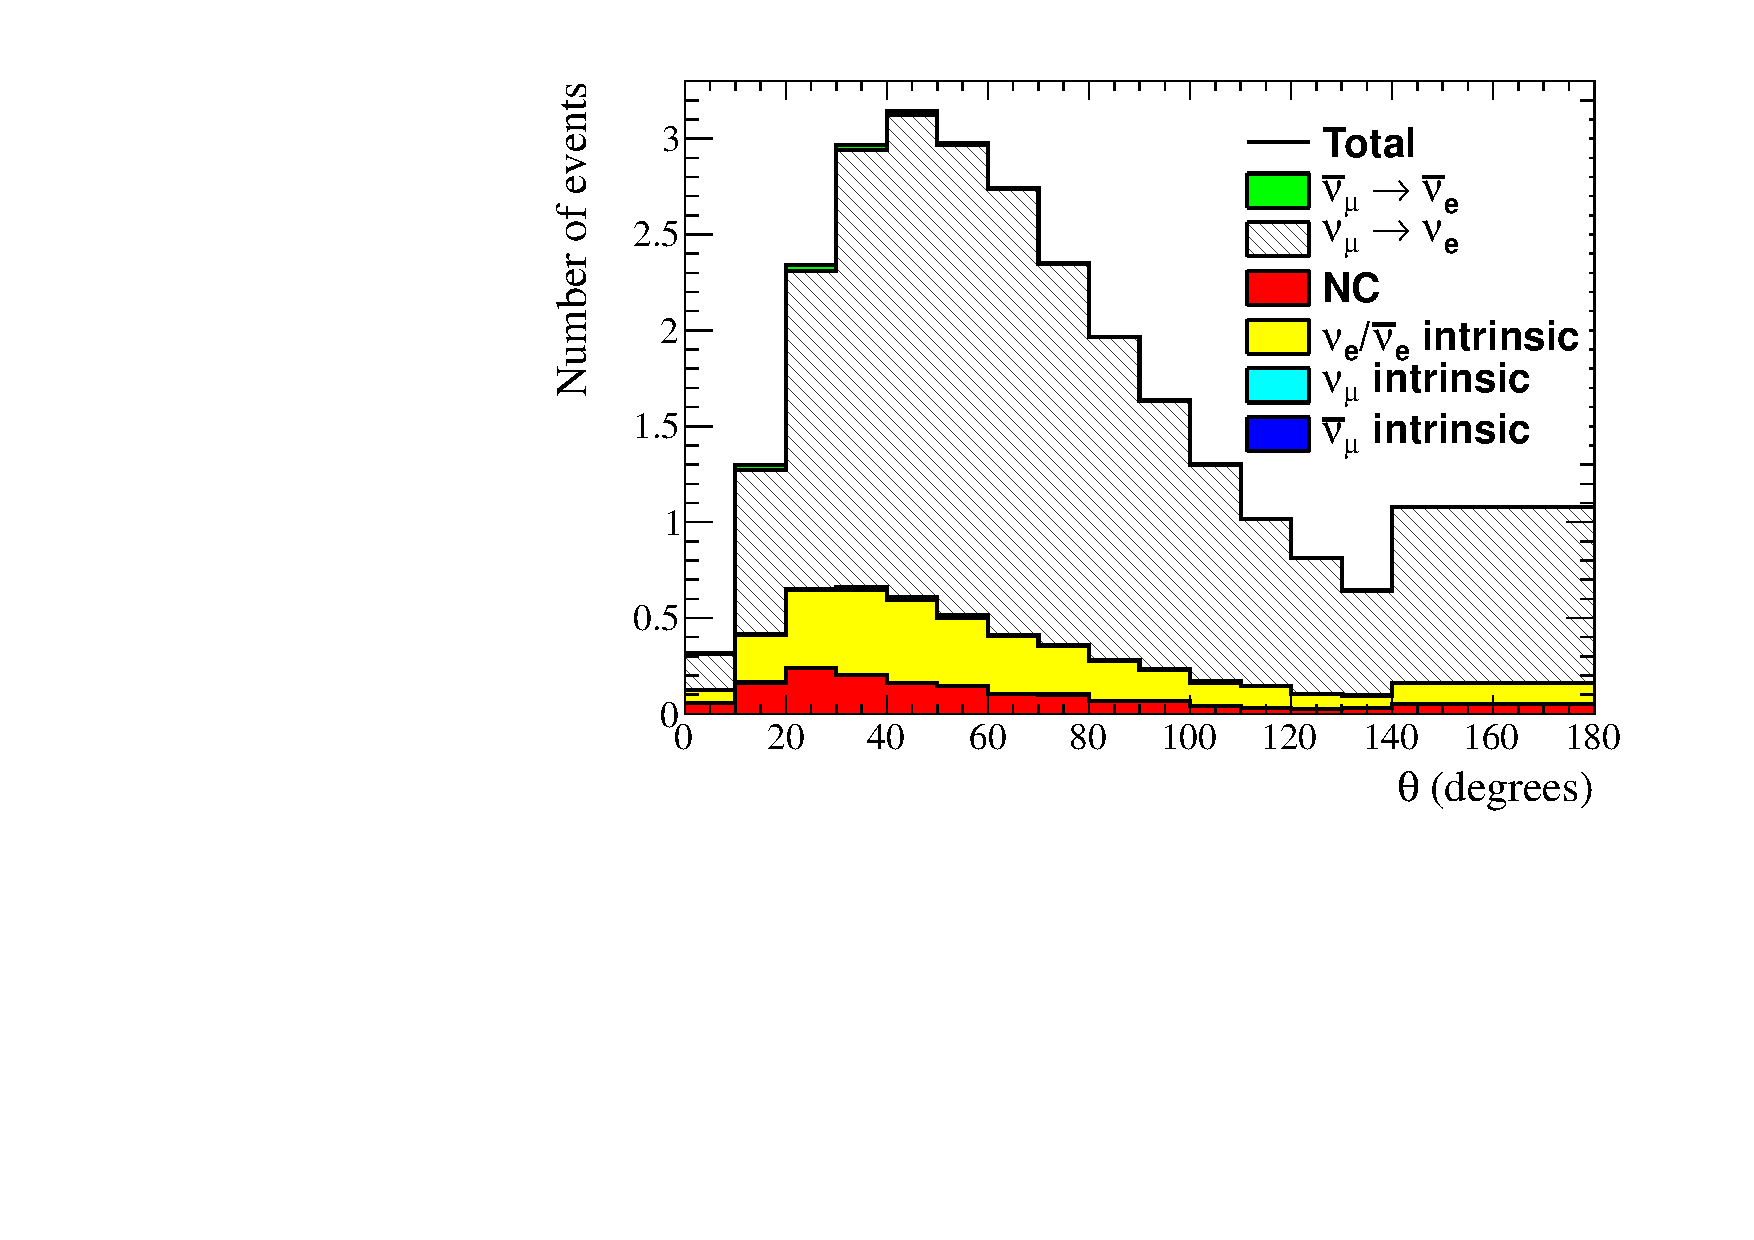
\includegraphics[width=18pc]{joint_plots/spectrum_predictions/template_theta_1re.pdf}
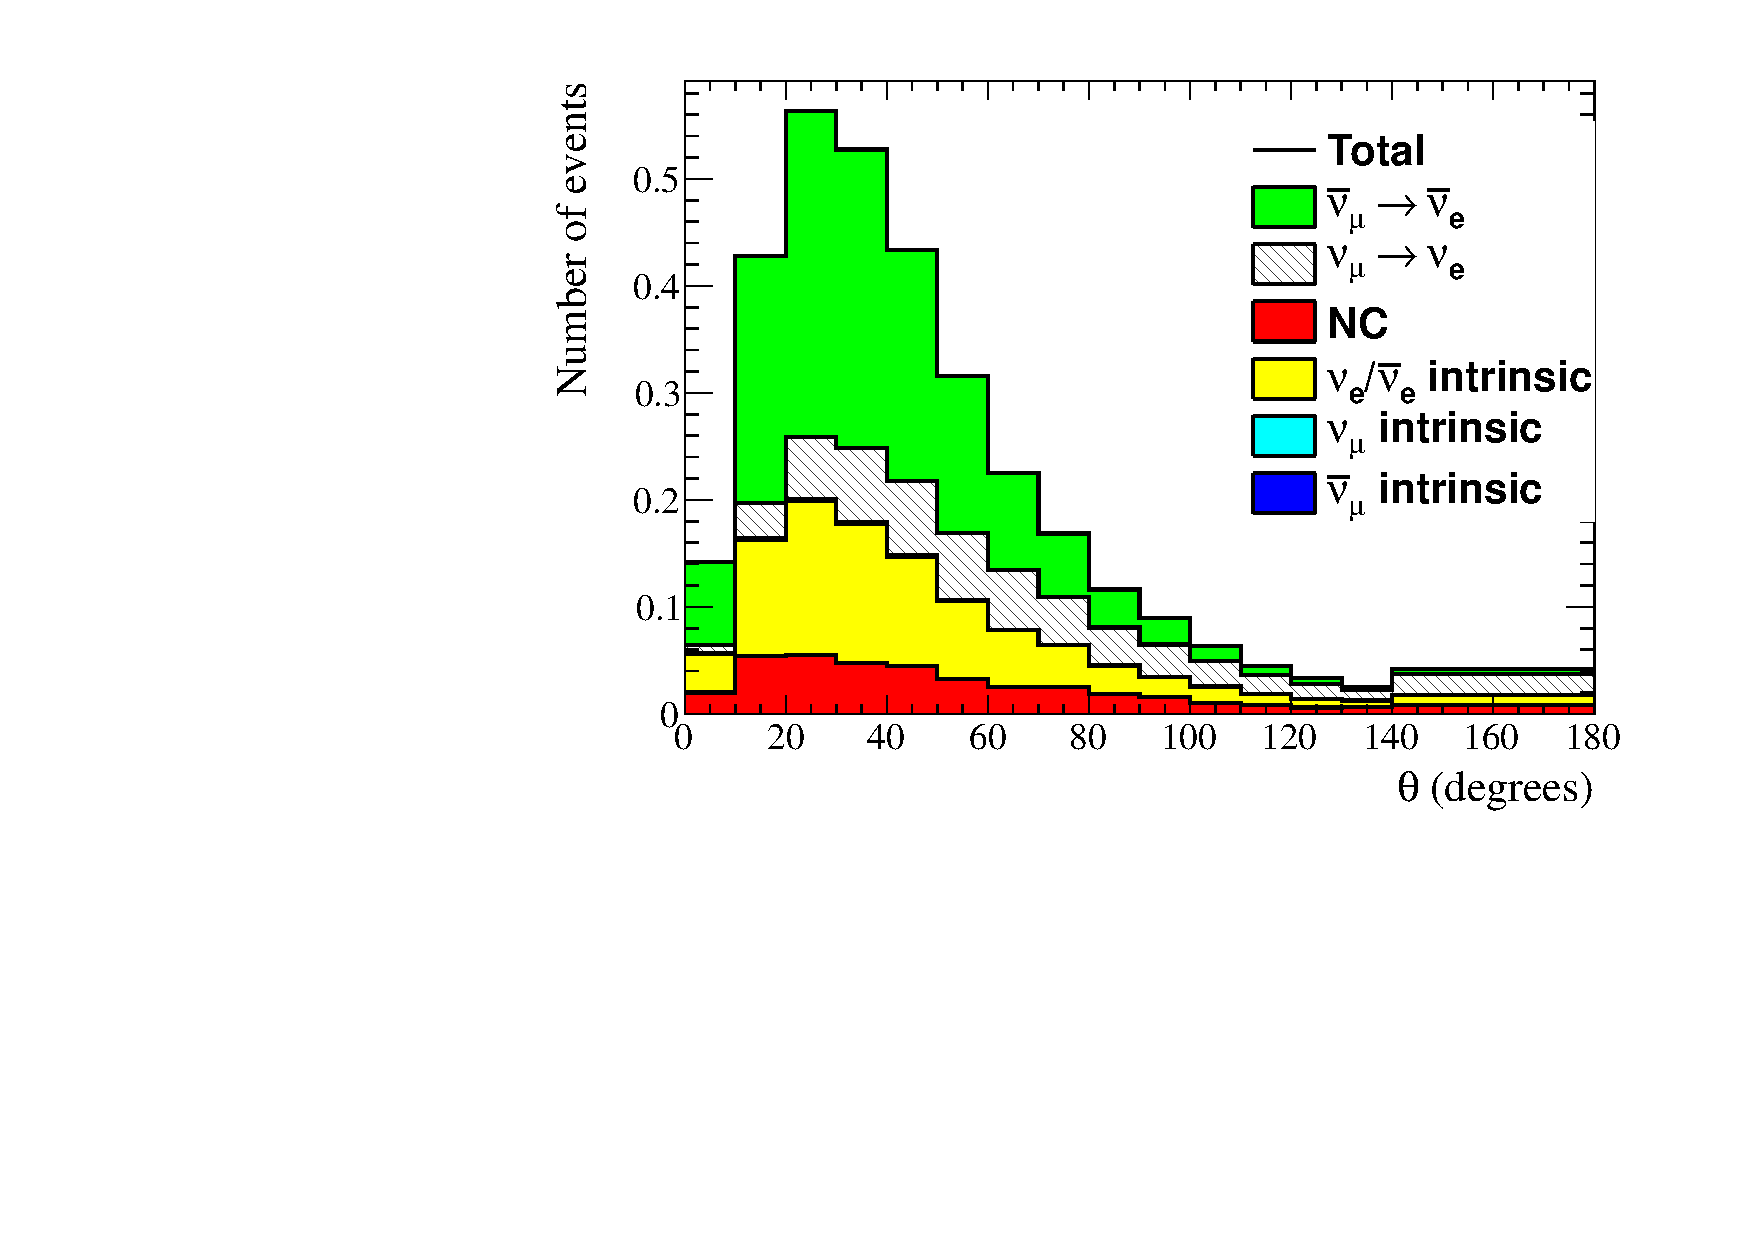
\includegraphics[width=18pc]{joint_plots/spectrum_predictions/template_theta_rhc1re.pdf}
\caption {
Predicted spectra of 
the reconstructed neutrino energy (top) 
and
the angle between the neutrino and the outgoing lepton directions (bottom)
for electron-like 
neutrino mode (left)
and
antineutrino mode (right)
events.
The distributions correspond to the collected statistics in the full Run 1-6 data set
for an exposure 
of $6.914 \times 10^{20}$ POT in neutrino mode
and
of $4.011 \times 10^{20}$ POT in antineutrino mode.
The distributions are broken down by the following components:
$\bar{\nu}_{\mu} \to \bar{\nu}_e$ (green), 
$\nu_{\mu} \to \nu_e$ (black/white), 
NC (red),
$\nu_e + \bar{\nu}_e$ intrinsic beam (yellow),
$\nu_{\mu}$ intrinsic beam (light blue)
and
$\bar{\nu}_{\mu}$ intrinsic beam (blue).
The spectra were generated with the systematic parameters measured with the ND280 data 
shown in tab.~\ref{tab:banff_uncertainties_flux_fhc},~\ref{tab:banff_uncertainties_flux_rhc},~\ref{tab:banff_uncertainties_xsec}
and \ref{tab:banff_uncertainties_skdetfsi}
and the oscillation parameters corresponding to the Asimov data set A shown in tab.~\ref{tab:osc_params_joint_asimov}.
}
\label{fig:joint_1d_elike}
\end{figure*}


%\clearpage


\clearpage


%...........................................................
%
% Observed spectra
%
%...........................................................

\section{Observed $e$-like spectra}
\label{app:templates_observed}

In Fig.~\ref{fig:joint_ereco_vs_theta_1re} and~\ref{fig:joint_ereco_vs_theta_rhc1re}
the predicted $e$-like 2-dimensional spectra are compared to data for
both neutrino and antineutrino beam mode.

\begin{figure*}[htb]
%\hspace{0.06\linewidth}
\center
%
\includegraphics[width=18pc]{./images/missing_plot-eps-converted-to.pdf}
%
\includegraphics[width=18pc]{./images/missing_plot-eps-converted-to.pdf}
%
\includegraphics[width=18pc]{./images/missing_plot-eps-converted-to.pdf}
%
\includegraphics[width=18pc]{./images/missing_plot-eps-converted-to.pdf}
%
\includegraphics[width=18pc]{./images/missing_plot-eps-converted-to.pdf}
%
\includegraphics[width=18pc]{./images/missing_plot-eps-converted-to.pdf}
%
\includegraphics[width=18pc]{./images/missing_plot-eps-converted-to.pdf}
\includegraphics[width=18pc]{./joint_plots/data/data_mc_1re_2d_NuMuToNue.pdf}
\includegraphics[width=18pc]{./joint_plots/data/data_mc_1re_2d_NuMuBarToNueBar.pdf}
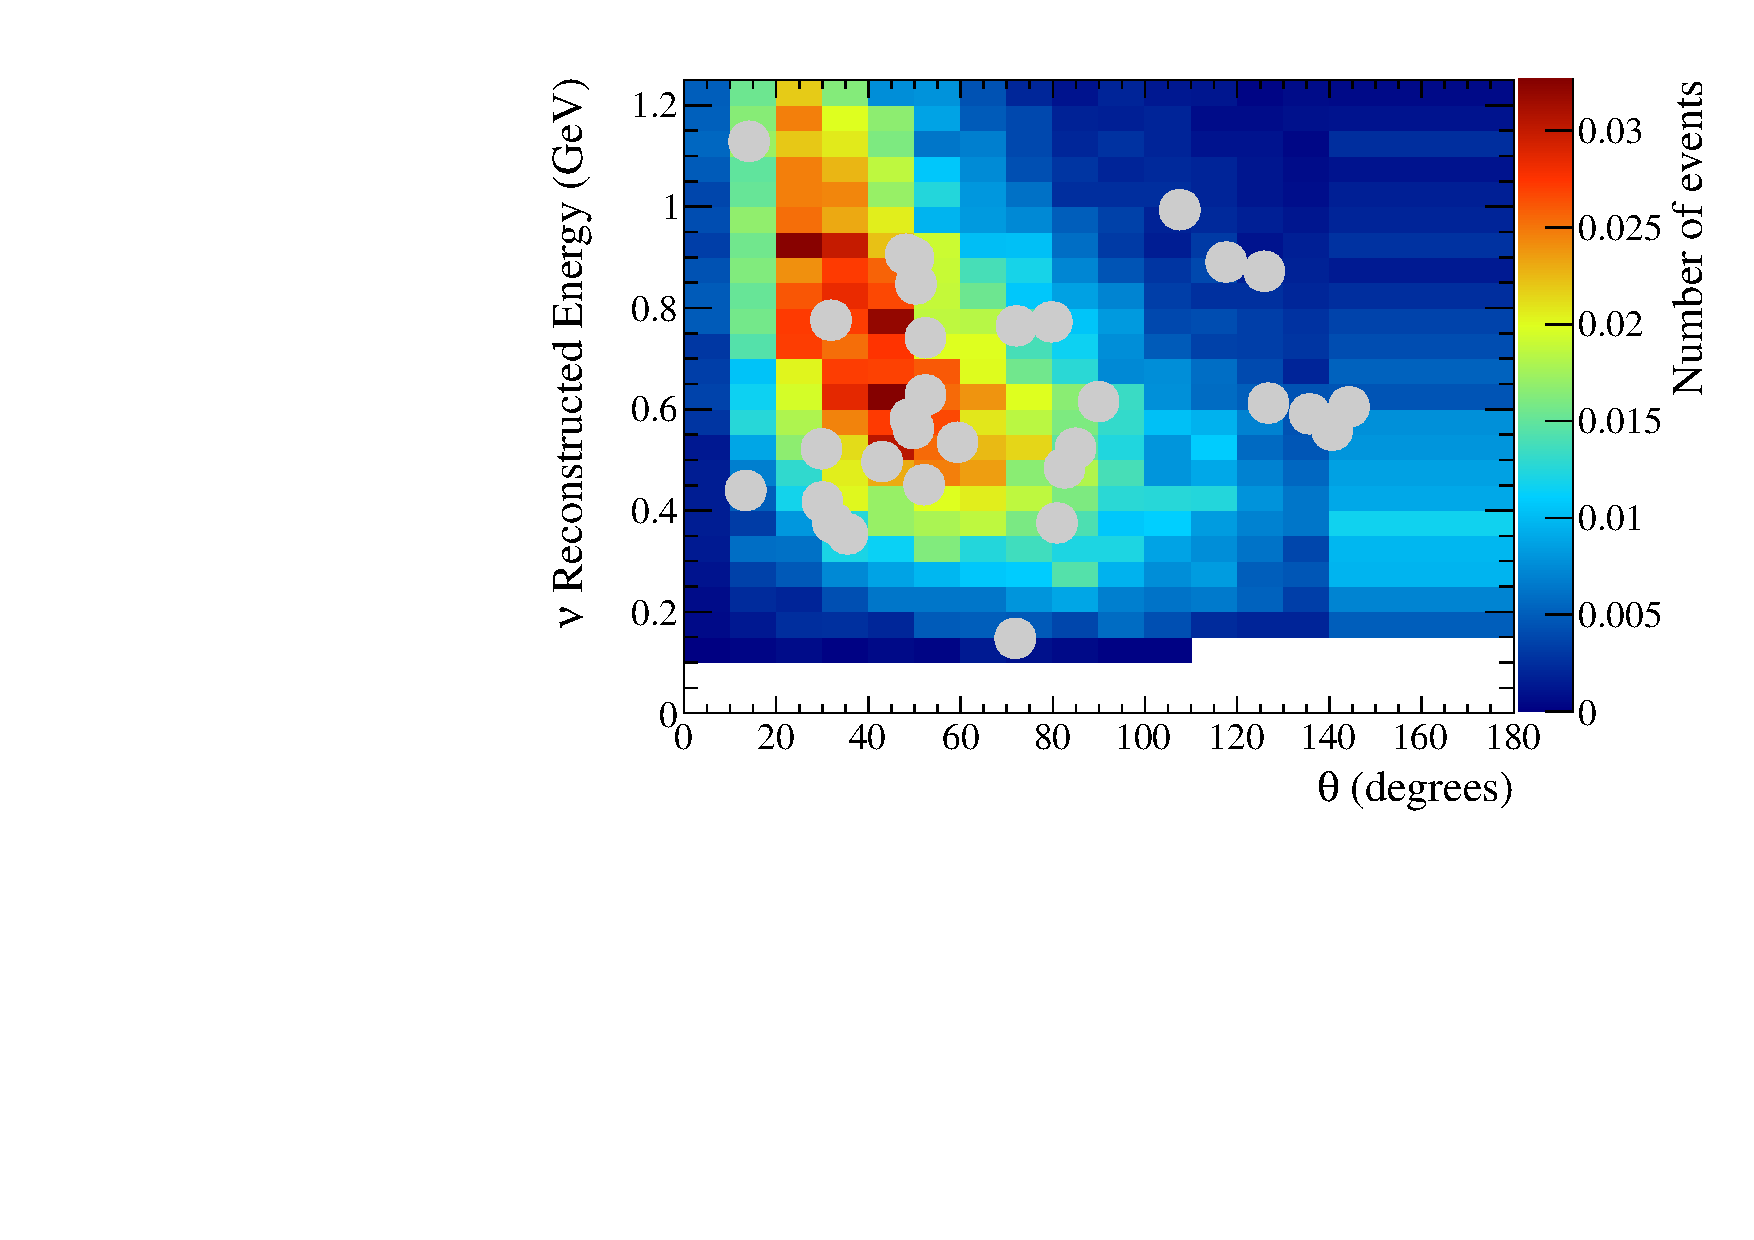
\includegraphics[width=18pc]{./joint_plots/data/data_mc_1re_2d_NueBeam.pdf}
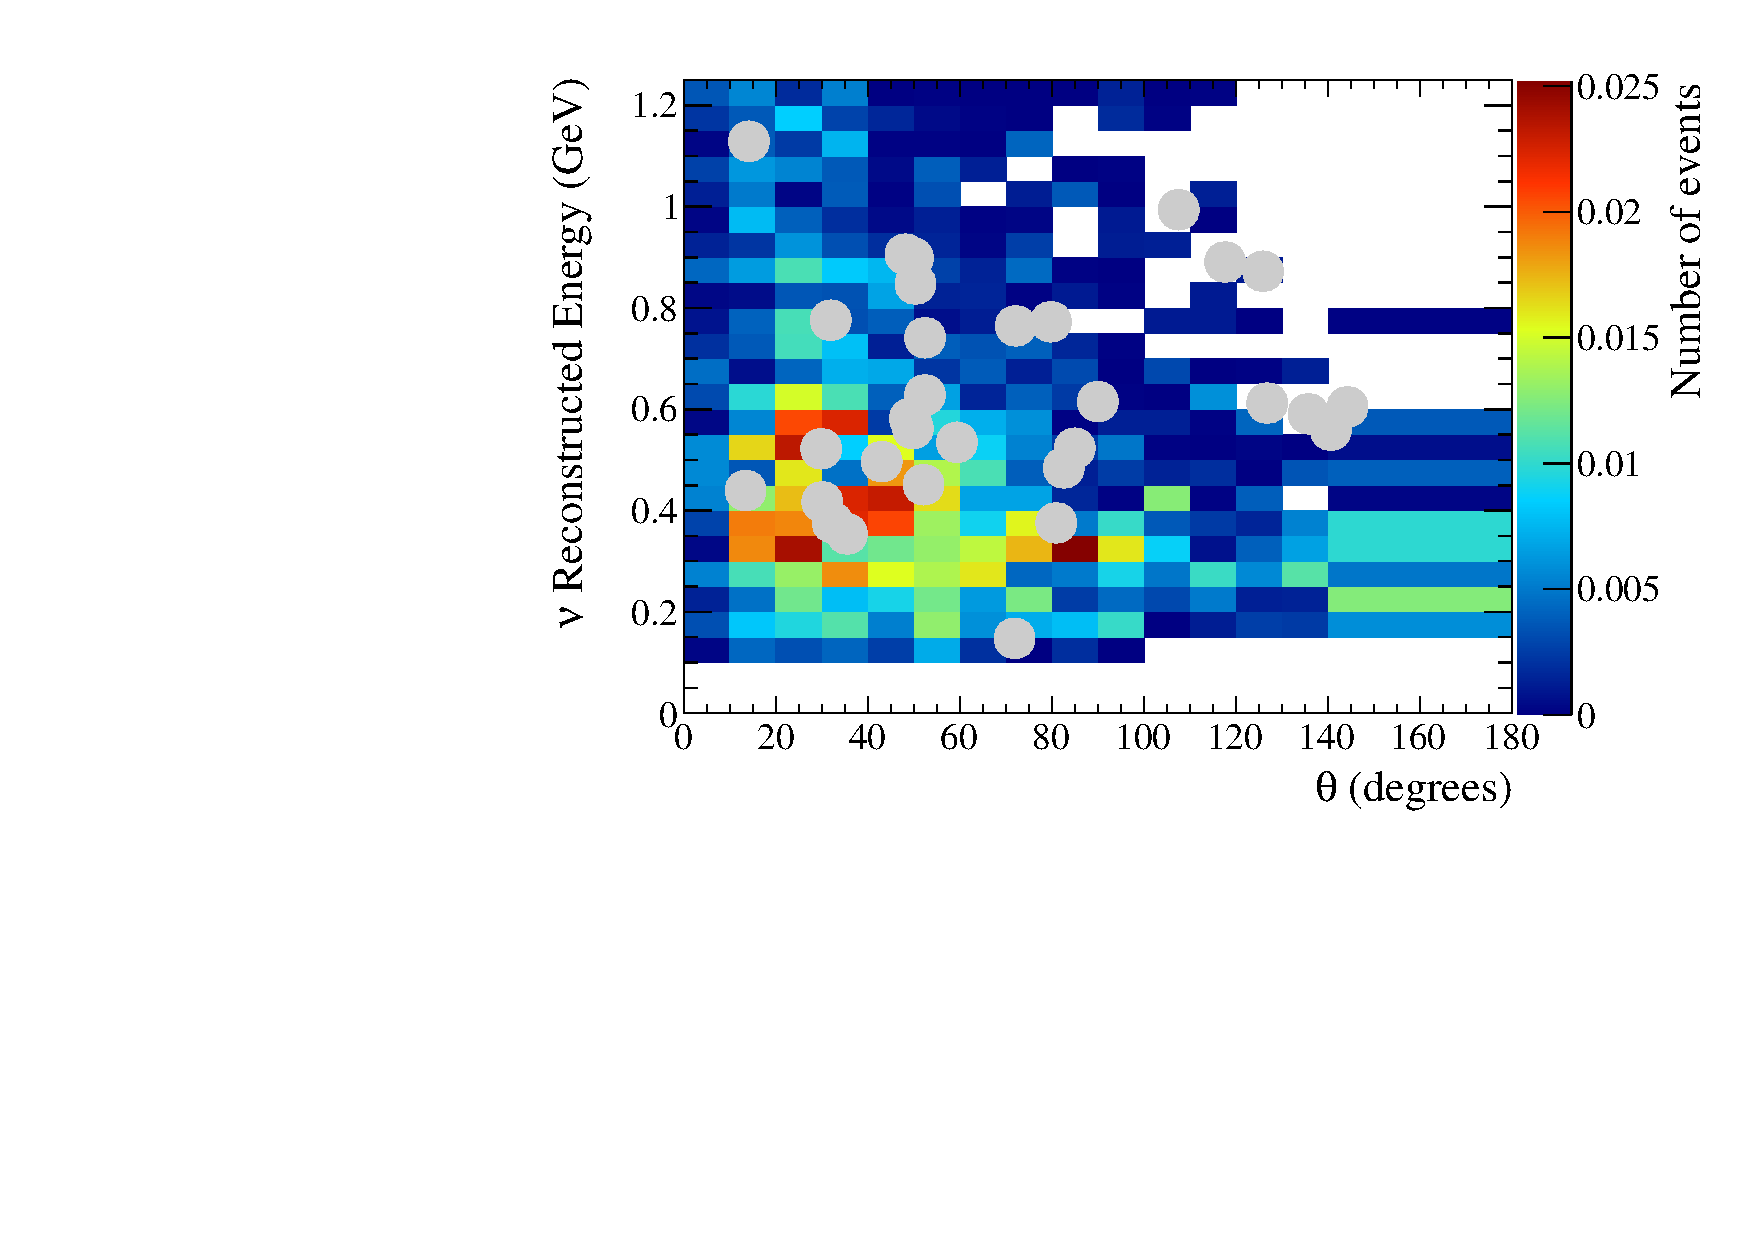
\includegraphics[width=18pc]{./joint_plots/data/data_mc_1re_2d_NC.pdf}
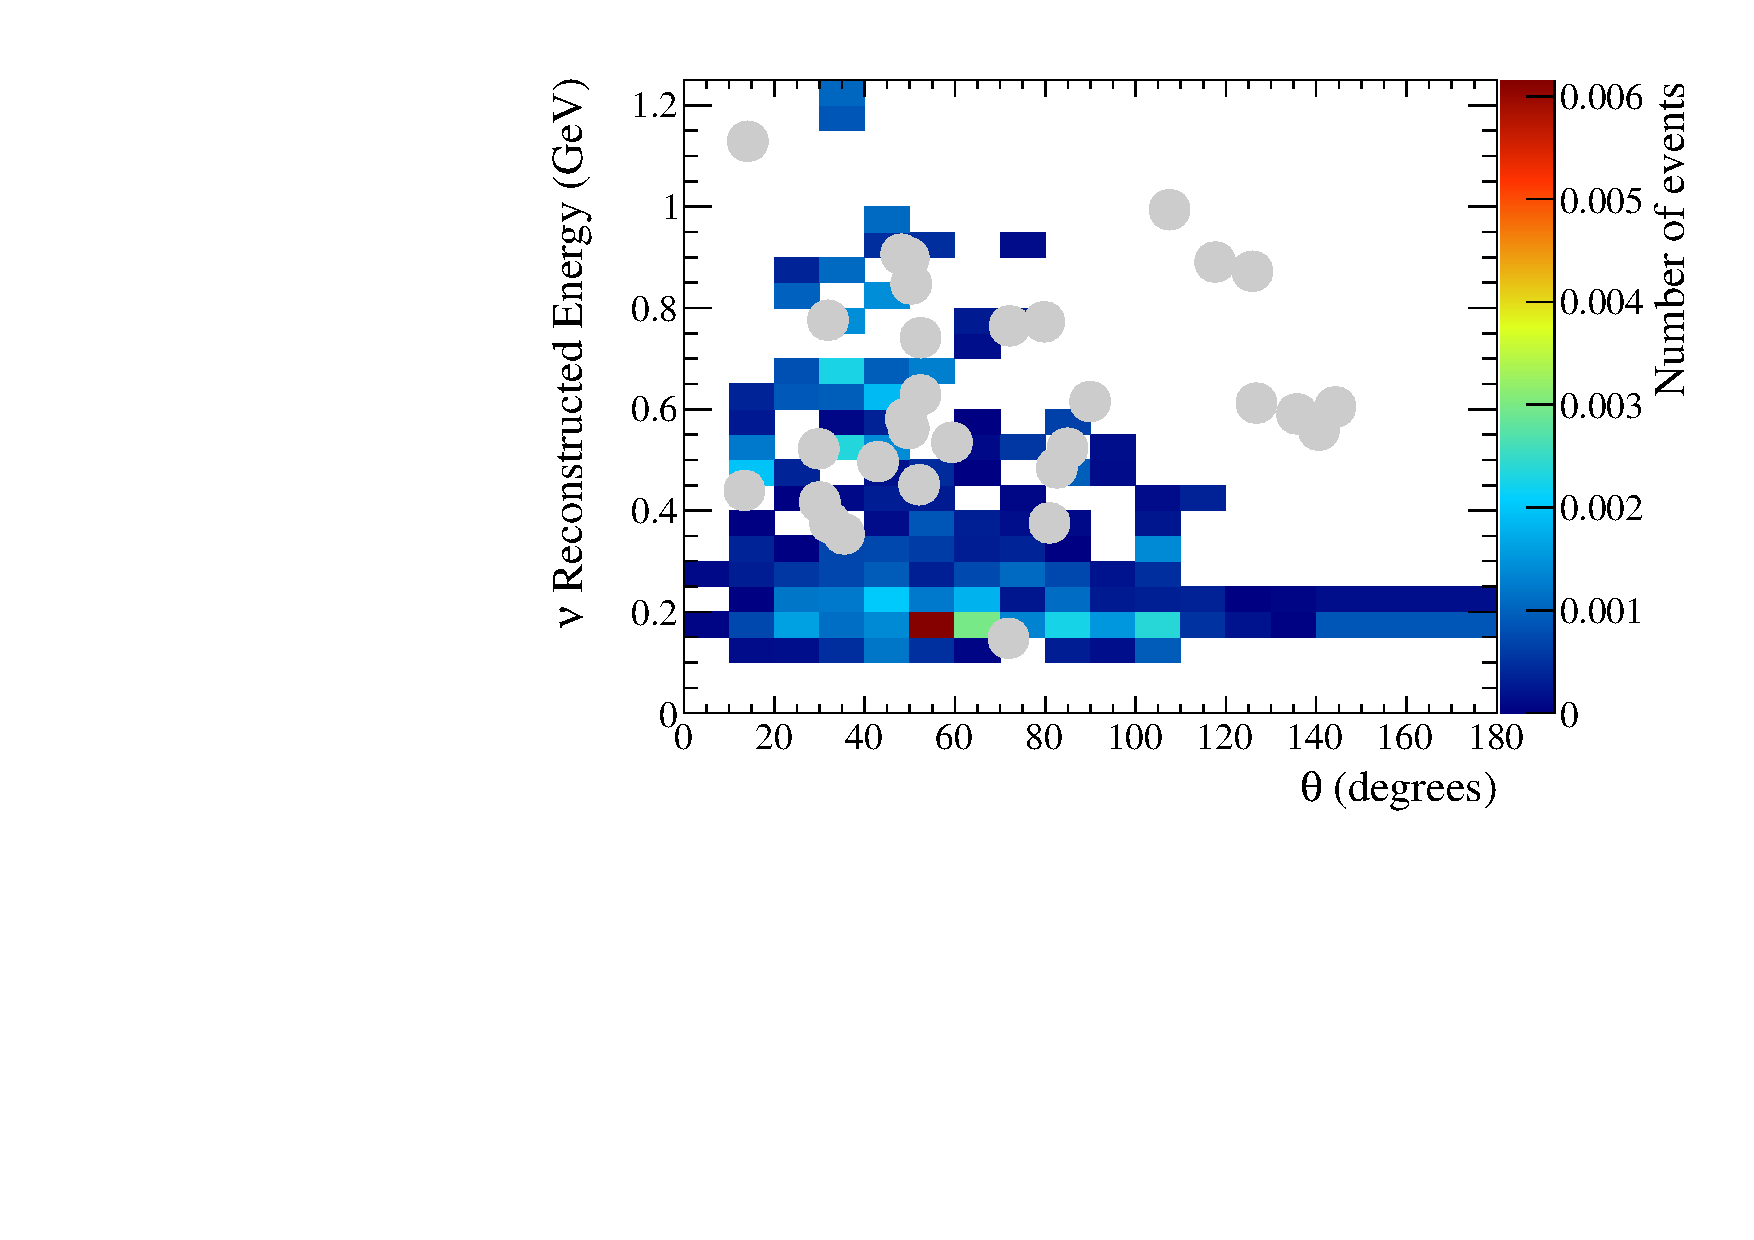
\includegraphics[width=18pc]{./joint_plots/data/data_mc_1re_2d_NumuBeam.pdf}
\includegraphics[width=18pc]{./joint_plots/data/data_mc_1re_2d_NumuBarBeam.pdf}

\caption {
Predicted and observed (grey dots) spectra of electron-like events
as a function of the reconstructed neutrino energy and
the angle between the outgoing lepton and the neutrino direction.
The distributions correspond to the collected statistics in the full Run 1-6 data set
for an exposure 
of $6.914 \times 10^{20}$ POT in neutrino mode.
%and
%of $4.011 \times 10^{20}$ POT in antineutrino mode.
From top left to bottom right the following components are shown:
total,
$\nu_{\mu} \rightarrow \nu_e$,
$\bar{\nu}_{\mu} \rightarrow \bar{\nu}_e$,
$\nu_e + \bar{\nu}_e$ intrinsic beam,
NC,
$\nu_{\mu}$ intrinsic beam
and
$\bar{\nu}_{\mu}$ intrinsic beam.
The spectra were generated with the systematic parameters measured with the ND280 data 
shown in tab.~\ref{tab:banff_uncertainties_flux_fhc},~\ref{tab:banff_uncertainties_flux_rhc},~\ref{tab:banff_uncertainties_xsec}
and \ref{tab:banff_uncertainties_skdetfsi}
and the oscillation parameters corresponding to the Asimov data set A shown in tab.~\ref{tab:osc_params_joint_asimov}.
}
\label{fig:joint_ereco_vs_theta_1re}
\end{figure*}

\begin{figure*}[htb]
%\hspace{0.06\linewidth}
\center
%\includegraphics[width=18pc]{./images/missing_plot-eps-converted-to.pdf}
%\includegraphics[width=18pc]{./images/missing_plot-eps-converted-to.pdf}
%\includegraphics[width=18pc]{./images/missing_plot-eps-converted-to.pdf}
%\includegraphics[width=18pc]{./images/missing_plot-eps-converted-to.pdf}
%\includegraphics[width=18pc]{./images/missing_plot-eps-converted-to.pdf}
%\includegraphics[width=18pc]{./images/missing_plot-eps-converted-to.pdf}
%\includegraphics[width=18pc]{./images/missing_plot-eps-converted-to.pdf}
\includegraphics[width=18pc]{./joint_plots/data/data_mc_rhc1re_2d_NuMuToNue.pdf}
\includegraphics[width=18pc]{./joint_plots/data/data_mc_rhc1re_2d_NuMuBarToNueBar.pdf}
\includegraphics[width=18pc]{./joint_plots/data/data_mc_rhc1re_2d_NueBeam.pdf}
\includegraphics[width=18pc]{./joint_plots/data/data_mc_rhc1re_2d_NC.pdf}
\includegraphics[width=18pc]{./joint_plots/data/data_mc_rhc1re_2d_NumuBeam.pdf}
\includegraphics[width=18pc]{./joint_plots/data/data_mc_rhc1re_2d_NumuBarBeam.pdf}
\caption {
Predicted and observed (grey dots) spectra of electron-like events
as a function of the reconstructed neutrino energy and
the angle between the outgoing lepton and the neutrino direction.
The distributions correspond to the collected statistics in the full Run 1-6 data set
for an exposure 
%of $6.914 \times 10^{20}$ POT in neutrino  mode.
%and
of $4.011 \times 10^{20}$ POT in antineutrino mode.
From top left to bottom right the following components are shown:
total,
$\nu_{\mu} \rightarrow \nu_e$,
$\bar{\nu}_{\mu} \rightarrow \bar{\nu}_e$,
$\nu_e + \bar{\nu}_e$ intrinsic beam,
NC,
$\nu_{\mu}$ intrinsic beam
and
$\bar{\nu}_{\mu}$ intrinsic beam.
The spectra were generated with the systematic parameters measured with the ND280 data 
shown in tab.~\ref{tab:banff_uncertainties_flux_fhc},~\ref{tab:banff_uncertainties_flux_rhc},~\ref{tab:banff_uncertainties_xsec}
and \ref{tab:banff_uncertainties_skdetfsi}
and the oscillation parameters corresponding to the Asimov data set A shown in tab.~\ref{tab:osc_params_joint_asimov}.
}
\label{fig:joint_ereco_vs_theta_rhc1re}
\end{figure*}


\clearpage




%...........................................................
%
% Predicted number of events
%
%...........................................................

\section{Effect of systematic uncertainties}
\label{app:systematics}

In \cref{tab:apply_syst_to_template_mulike_fhc},
\cref{tab:apply_syst_to_template_elike_fhc},
\cref{tab:apply_syst_to_template_mulike_rhc} and
\cref{tab:apply_syst_to_template_elike_fhc}
it is shown which systematic parameter is applied to which reaction and flavour modes 
for all the Super-K samples.
 
\afterpage{%\documentclass[10pt]{article}
%\usepackage[utf8]{inputenc}
%\usepackage{amsmath}
%\usepackage{amsfonts}
%\usepackage{amssymb}
%\usepackage{fullpage}
%\usepackage{rotate}  
%\usepackage{rotating}
%\usepackage[paperwidth=300mm,paperheight=450mm]{geometry}

%\newcommand{\ck}{$\checkmark$}
%\begin{document}

{
\setlength{\tabcolsep}{2pt}
\renewcommand{\arraystretch}{1.5}
\begin{landscape}
\begin{footnotesize}

\begin{longtable} { | c ||c | c | c | c | c | c | c | c | c | c | c | c | c | c | c | c | c | c | c | c | c | c | c | c | c | c | c | c | c | c | c | c | c | c | c | c | c | c | c | c | c | c | c | c | c | c | c | c | c | c |  | }
\hline
 & \begin{sideways} $\nu_\mu$ CCQE \end{sideways} 
 & \begin{sideways} $\nu_\mu$ CC 1$\pi$ \end{sideways} 
 & \begin{sideways} $\nu_\mu$ CC coherent \end{sideways} 
 & \begin{sideways} $\nu_\mu$ CC 2p-2h \end{sideways} 
 & \begin{sideways} $\nu_\mu$ CC other \end{sideways} 
 & \begin{sideways} $\nu_\mu$/$\nu_\tau$ NC 1$\pi^{+/-}$ \end{sideways} 
 & \begin{sideways} $\nu_\mu$/$\nu_\tau$ NC 1$\pi^0$ \end{sideways} 
 & \begin{sideways} $\nu_\mu$/$\nu_\tau$ NC coherent \end{sideways} 
 & \begin{sideways} $\nu_\mu$/$\nu_\tau$ NC other \end{sideways} 
 & \begin{sideways} $\nu_e$ NC 1$\gamma$ \end{sideways} 
 & \begin{sideways} $\bar{\nu}_\mu$ CCQE \end{sideways} 
 & \begin{sideways} $\bar{\nu}_\mu$ CC 1$\pi$ \end{sideways} 
 & \begin{sideways} $\bar{\nu}_\mu$ CC coherent \end{sideways} 
 & \begin{sideways} $\bar{\nu}_\mu$ CC 2p-2h \end{sideways} 
 & \begin{sideways} $\bar{\nu}_\mu$ CC other \end{sideways} 
 & \begin{sideways} $\bar{\nu}_\mu$/$\bar{\nu}_\tau$ NC 1$\pi^{+/-}$ \end{sideways} 
 & \begin{sideways} $\bar{\nu}_\mu$/$\bar{\nu}_\tau$ NC 1$\pi^0$ \end{sideways} 
 & \begin{sideways} $\bar{\nu}_\mu$/$\bar{\nu}_\tau$ NC coherent \end{sideways} 
 & \begin{sideways} $\bar{\nu}_\mu$/$\bar{\nu}_\tau$ NC other \end{sideways} 
 & \begin{sideways} $\nu_\mu$ NC 1$\gamma$ \end{sideways} 
 & \begin{sideways} $\nu_e$ CCQE \end{sideways} 
 & \begin{sideways} $\nu_e$ CC 1$\pi$ \end{sideways} 
 & \begin{sideways} $\nu_e$ CC coherent \end{sideways} 
 & \begin{sideways} $\nu_e$ CC 2p-2h \end{sideways} 
 & \begin{sideways} $\nu_e$ CC other \end{sideways} 
 & \begin{sideways} $\nu_e$ NC 1$\pi^{+/-}$ \end{sideways} 
 & \begin{sideways} $\nu_e$ NC 1$\pi^0$ \end{sideways} 
 & \begin{sideways} $\nu_e$ NC coherent \end{sideways} 
 & \begin{sideways} $\nu_e$ NC other \end{sideways} 
 & \begin{sideways} $\bar{\nu}_\mu$ NC 1$\gamma$ \end{sideways} 
 & \begin{sideways} Osc. $\nu_e$ CCQE \end{sideways} 
 & \begin{sideways} Osc. $\nu_e$ CC 1$\pi$ \end{sideways} 
 & \begin{sideways} Osc. $\nu_e$ CC coherent \end{sideways} 
 & \begin{sideways} Osc. $\nu_e$ CC 2p-2h \end{sideways} 
 & \begin{sideways} Osc. $\nu_e$ CC other \end{sideways} 
 & \begin{sideways} $\bar{\nu}_e$ CCQE \end{sideways} 
 & \begin{sideways} $\bar{\nu}_e$ CC 1$\pi$ \end{sideways} 
 & \begin{sideways} $\bar{\nu}_e$ CC coherent \end{sideways} 
 & \begin{sideways} $\bar{\nu}_e$ CC 2p-2h \end{sideways} 
 & \begin{sideways} $\bar{\nu}_e$ CC other \end{sideways} 
 & \begin{sideways} $\bar{\nu}_e$ NC 1$\pi^{+/-}$ \end{sideways} 
 & \begin{sideways} $\bar{\nu}_e$ NC 1$\pi^0$ \end{sideways} 
 & \begin{sideways} $\bar{\nu}_e$ NC coherent \end{sideways} 
 & \begin{sideways} $\bar{\nu}_e$ NC other \end{sideways} 
 & \begin{sideways} $\bar{\nu}_e$ NC 1$\gamma$ \end{sideways} 
 & \begin{sideways} Osc. $\bar{\nu}_e$ CCQE \end{sideways} 
 & \begin{sideways} Osc. $\bar{\nu}_e$ CC 1$\pi$ \end{sideways} 
 & \begin{sideways} Osc. $\bar{\nu}_e$ CC coherent \end{sideways} 
 & \begin{sideways} Osc. $\bar{\nu}_e$ CC 2p-2h \end{sideways} 
 & \begin{sideways} Osc. $\bar{\nu}_e$ CC other \end{sideways} 
\\ \hline 
%$\sin^2(\theta_{12})$         & \ck& \ck& \ck& \ck& \ck&    &    &    &    &    & \ck& \ck& \ck& \ck& \ck&    &    &    &    &    & \ck& \ck& \ck& \ck& \ck&    &    &    &    &    & \ck& \ck& \ck& \ck& \ck& \ck& \ck& \ck& \ck& \ck&    &    &    &    &    & \ck& \ck& \ck& \ck& \ck \\ \hline 
%$\sin^2(\theta_{13})$         & \ck& \ck& \ck& \ck& \ck&    &    &    &    &    & \ck& \ck& \ck& \ck& \ck&    &    &    &    &    & \ck& \ck& \ck& \ck& \ck&    &    &    &    &    & \ck& \ck& \ck& \ck& \ck& \ck& \ck& \ck& \ck& \ck&    &    &    &    &    & \ck& \ck& \ck& \ck& \ck \\ \hline 
%$\Delta m^2_{21}$             & \ck& \ck& \ck& \ck& \ck&    &    &    &    &    & \ck& \ck& \ck& \ck& \ck&    &    &    &    &    & \ck& \ck& \ck& \ck& \ck&    &    &    &    &    & \ck& \ck& \ck& \ck& \ck& \ck& \ck& \ck& \ck& \ck&    &    &    &    &    & \ck& \ck& \ck& \ck& \ck \\ \hline 
%$\delta_{CP}$                 & \ck& \ck& \ck& \ck& \ck&    &    &    &    &    & \ck& \ck& \ck& \ck& \ck&    &    &    &    &    & \ck& \ck& \ck& \ck& \ck&    &    &    &    &    & \ck& \ck& \ck& \ck& \ck& \ck& \ck& \ck& \ck& \ck&    &    &    &    &    & \ck& \ck& \ck& \ck& \ck \\ \hline 
$f_{E; r}^{SK}$               & \ck& \ck& \ck& \ck& \ck& \ck& \ck& \ck& \ck& \ck& \ck& \ck& \ck& \ck& \ck& \ck& \ck& \ck& \ck& \ck& \ck& \ck& \ck& \ck& \ck& \ck& \ck& \ck& \ck& \ck& \ck& \ck& \ck& \ck& \ck& \ck& \ck& \ck& \ck& \ck& \ck& \ck& \ck& \ck& \ck& \ck& \ck& \ck& \ck& \ck \\ \hline 
$f_{0; t, r}^{SK+FSI}$        & \ck&    &    & \ck&    &    &    &    &    &    & \ck&    &    & \ck&    &    &    &    &    &    &    &    &    &    &    &    &    &    &    &    &    &    &    &    &    &    &    &    &    &    &    &    &    &    &    &    &    &    &    &     \\ \hline 
$f_{1; t, r}^{SK+FSI}$        & \ck&    &    & \ck&    &    &    &    &    &    & \ck&    &    & \ck&    &    &    &    &    &    &    &    &    &    &    &    &    &    &    &    &    &    &    &    &    &    &    &    &    &    &    &    &    &    &    &    &    &    &    &     \\ \hline 
$f_{2; t, r}^{SK+FSI}$        & \ck&    &    & \ck&    &    &    &    &    &    & \ck&    &    & \ck&    &    &    &    &    &    &    &    &    &    &    &    &    &    &    &    &    &    &    &    &    &    &    &    &    &    &    &    &    &    &    &    &    &    &    &     \\ \hline 
$f_{3; t, r}^{SK+FSI}$        &    & \ck& \ck&    & \ck&    &    &    &    &    &    & \ck& \ck&    & \ck&    &    &    &    &    &    &    &    &    &    &    &    &    &    &    &    &    &    &    &    &    &    &    &    &    &    &    &    &    &    &    &    &    &    &     \\ \hline 
$f_{4; t, r}^{SK+FSI}$        &    &    &    &    &    &    &    &    &    &    &    &    &    &    &    &    &    &    &    &    & \ck& \ck& \ck& \ck& \ck&    &    &    &    &    & \ck& \ck& \ck& \ck& \ck& \ck& \ck& \ck& \ck& \ck&    &    &    &    &    & \ck& \ck& \ck& \ck& \ck \\ \hline 
$f_{5; t, r}^{SK+FSI}$        &    &    &    &    &    & \ck& \ck& \ck& \ck& \ck&    &    &    &    &    & \ck& \ck& \ck& \ck& \ck&    &    &    &    &    & \ck& \ck& \ck& \ck& \ck&    &    &    &    &    &    &    &    &    &    & \ck& \ck& \ck& \ck& \ck&    &    &    &    &     \\ \hline 
$f_{0; t, r}^{banff}$         & \ck& \ck& \ck& \ck& \ck& \ck& \ck& \ck& \ck& \ck&    &    &    &    &    &    &    &    &    &    &    &    &    &    &    &    &    &    &    &    & \ck& \ck& \ck& \ck& \ck&    &    &    &    &    &    &    &    &    &    &    &    &    &    &     \\ \hline 
$f_{1; t, r}^{banff}$         & \ck& \ck& \ck& \ck& \ck& \ck& \ck& \ck& \ck& \ck&    &    &    &    &    &    &    &    &    &    &    &    &    &    &    &    &    &    &    &    & \ck& \ck& \ck& \ck& \ck&    &    &    &    &    &    &    &    &    &    &    &    &    &    &     \\ \hline 
$f_{2; t, r}^{banff}$         & \ck& \ck& \ck& \ck& \ck& \ck& \ck& \ck& \ck& \ck&    &    &    &    &    &    &    &    &    &    &    &    &    &    &    &    &    &    &    &    & \ck& \ck& \ck& \ck& \ck&    &    &    &    &    &    &    &    &    &    &    &    &    &    &     \\ \hline 
$f_{3; t, r}^{banff}$         & \ck& \ck& \ck& \ck& \ck& \ck& \ck& \ck& \ck& \ck&    &    &    &    &    &    &    &    &    &    &    &    &    &    &    &    &    &    &    &    & \ck& \ck& \ck& \ck& \ck&    &    &    &    &    &    &    &    &    &    &    &    &    &    &     \\ \hline 
$f_{4; t, r}^{banff}$         & \ck& \ck& \ck& \ck& \ck& \ck& \ck& \ck& \ck& \ck&    &    &    &    &    &    &    &    &    &    &    &    &    &    &    &    &    &    &    &    & \ck& \ck& \ck& \ck& \ck&    &    &    &    &    &    &    &    &    &    &    &    &    &    &     \\ \hline 
$f_{5; t, r}^{banff}$         & \ck& \ck& \ck& \ck& \ck& \ck& \ck& \ck& \ck& \ck&    &    &    &    &    &    &    &    &    &    &    &    &    &    &    &    &    &    &    &    & \ck& \ck& \ck& \ck& \ck&    &    &    &    &    &    &    &    &    &    &    &    &    &    &     \\ \hline 
$f_{6; t, r}^{banff}$         & \ck& \ck& \ck& \ck& \ck& \ck& \ck& \ck& \ck& \ck&    &    &    &    &    &    &    &    &    &    &    &    &    &    &    &    &    &    &    &    & \ck& \ck& \ck& \ck& \ck&    &    &    &    &    &    &    &    &    &    &    &    &    &    &     \\ \hline 
$f_{7; t, r}^{banff}$         & \ck& \ck& \ck& \ck& \ck& \ck& \ck& \ck& \ck& \ck&    &    &    &    &    &    &    &    &    &    &    &    &    &    &    &    &    &    &    &    & \ck& \ck& \ck& \ck& \ck&    &    &    &    &    &    &    &    &    &    &    &    &    &    &     \\ \hline 
$f_{8; t, r}^{banff}$         & \ck& \ck& \ck& \ck& \ck& \ck& \ck& \ck& \ck& \ck&    &    &    &    &    &    &    &    &    &    &    &    &    &    &    &    &    &    &    &    & \ck& \ck& \ck& \ck& \ck&    &    &    &    &    &    &    &    &    &    &    &    &    &    &     \\ \hline 
$f_{9; t, r}^{banff}$         & \ck& \ck& \ck& \ck& \ck& \ck& \ck& \ck& \ck& \ck&    &    &    &    &    &    &    &    &    &    &    &    &    &    &    &    &    &    &    &    & \ck& \ck& \ck& \ck& \ck&    &    &    &    &    &    &    &    &    &    &    &    &    &    &     \\ \hline 
$f_{10; t, r}^{banff}$        & \ck& \ck& \ck& \ck& \ck& \ck& \ck& \ck& \ck& \ck&    &    &    &    &    &    &    &    &    &    &    &    &    &    &    &    &    &    &    &    & \ck& \ck& \ck& \ck& \ck&    &    &    &    &    &    &    &    &    &    &    &    &    &    &     \\ \hline 
$f_{11; t, r}^{banff}$        &    &    &    &    &    &    &    &    &    &    & \ck& \ck& \ck& \ck& \ck& \ck& \ck& \ck& \ck& \ck&    &    &    &    &    &    &    &    &    &    &    &    &    &    &    &    &    &    &    &    &    &    &    &    &    & \ck& \ck& \ck& \ck& \ck \\ \hline 
$f_{12; t, r}^{banff}$        &    &    &    &    &    &    &    &    &    &    & \ck& \ck& \ck& \ck& \ck& \ck& \ck& \ck& \ck& \ck&    &    &    &    &    &    &    &    &    &    &    &    &    &    &    &    &    &    &    &    &    &    &    &    &    & \ck& \ck& \ck& \ck& \ck \\ \hline 
$f_{13; t, r}^{banff}$        &    &    &    &    &    &    &    &    &    &    & \ck& \ck& \ck& \ck& \ck& \ck& \ck& \ck& \ck& \ck&    &    &    &    &    &    &    &    &    &    &    &    &    &    &    &    &    &    &    &    &    &    &    &    &    & \ck& \ck& \ck& \ck& \ck \\ \hline 
$f_{14; t, r}^{banff}$        &    &    &    &    &    &    &    &    &    &    & \ck& \ck& \ck& \ck& \ck& \ck& \ck& \ck& \ck& \ck&    &    &    &    &    &    &    &    &    &    &    &    &    &    &    &    &    &    &    &    &    &    &    &    &    & \ck& \ck& \ck& \ck& \ck \\ \hline 
$f_{15; t, r}^{banff}$        &    &    &    &    &    &    &    &    &    &    & \ck& \ck& \ck& \ck& \ck& \ck& \ck& \ck& \ck& \ck&    &    &    &    &    &    &    &    &    &    &    &    &    &    &    &    &    &    &    &    &    &    &    &    &    & \ck& \ck& \ck& \ck& \ck \\ \hline 
$f_{16; t, r}^{banff}$        &    &    &    &    &    &    &    &    &    &    &    &    &    &    &    &    &    &    &    &    & \ck& \ck& \ck& \ck& \ck& \ck& \ck& \ck& \ck& \ck&    &    &    &    &    &    &    &    &    &    &    &    &    &    &    &    &    &    &    &     \\ \hline 
$f_{17; t, r}^{banff}$        &    &    &    &    &    &    &    &    &    &    &    &    &    &    &    &    &    &    &    &    & \ck& \ck& \ck& \ck& \ck& \ck& \ck& \ck& \ck& \ck&    &    &    &    &    &    &    &    &    &    &    &    &    &    &    &    &    &    &    &     \\ \hline 
$f_{18; t, r}^{banff}$        &    &    &    &    &    &    &    &    &    &    &    &    &    &    &    &    &    &    &    &    & \ck& \ck& \ck& \ck& \ck& \ck& \ck& \ck& \ck& \ck&    &    &    &    &    &    &    &    &    &    &    &    &    &    &    &    &    &    &    &     \\ \hline 
$f_{19; t, r}^{banff}$        &    &    &    &    &    &    &    &    &    &    &    &    &    &    &    &    &    &    &    &    & \ck& \ck& \ck& \ck& \ck& \ck& \ck& \ck& \ck& \ck&    &    &    &    &    &    &    &    &    &    &    &    &    &    &    &    &    &    &    &     \\ \hline 
$f_{20; t, r}^{banff}$        &    &    &    &    &    &    &    &    &    &    &    &    &    &    &    &    &    &    &    &    & \ck& \ck& \ck& \ck& \ck& \ck& \ck& \ck& \ck& \ck&    &    &    &    &    &    &    &    &    &    &    &    &    &    &    &    &    &    &    &     \\ \hline 
$f_{21; t, r}^{banff}$        &    &    &    &    &    &    &    &    &    &    &    &    &    &    &    &    &    &    &    &    & \ck& \ck& \ck& \ck& \ck& \ck& \ck& \ck& \ck& \ck&    &    &    &    &    &    &    &    &    &    &    &    &    &    &    &    &    &    &    &     \\ \hline 
$f_{22; t, r}^{banff}$        &    &    &    &    &    &    &    &    &    &    &    &    &    &    &    &    &    &    &    &    & \ck& \ck& \ck& \ck& \ck& \ck& \ck& \ck& \ck& \ck&    &    &    &    &    &    &    &    &    &    &    &    &    &    &    &    &    &    &    &     \\ \hline 
$f_{23; t, r}^{banff}$        &    &    &    &    &    &    &    &    &    &    &    &    &    &    &    &    &    &    &    &    &    &    &    &    &    &    &    &    &    &    &    &    &    &    &    & \ck& \ck& \ck& \ck& \ck& \ck& \ck& \ck& \ck& \ck&    &    &    &    &     \\ \hline 
$f_{24; t, r}^{banff}$        &    &    &    &    &    &    &    &    &    &    &    &    &    &    &    &    &    &    &    &    &    &    &    &    &    &    &    &    &    &    &    &    &    &    &    & \ck& \ck& \ck& \ck& \ck& \ck& \ck& \ck& \ck& \ck&    &    &    &    &     \\ \hline 
$f_{M_A^{QE}}^{banff}$        & \ck&    &    &    &    &    &    &    &    &    & \ck&    &    &    &    &    &    &    &    &    & \ck&    &    &    &    &    &    &    &    &    & \ck&    &    &    &    & \ck&    &    &    &    &    &    &    &    &    & \ck&    &    &    &     \\ \hline 
$f_{M_A^{RES}}^{banff}$       &    & \ck&    &    &    & \ck& \ck&    &    &    &    & \ck&    &    &    & \ck& \ck&    &    &    &    & \ck&    &    &    & \ck& \ck&    &    &    &    & \ck&    &    &    &    & \ck&    &    &    & \ck& \ck&    &    &    &    & \ck&    &    &     \\ \hline 
$f_{Norm_{2p-2h}}^{banff}$      &    &    &    & \ck&    &    &    &    &    &    &    &    &    & \ck&    &    &    &    &    &    &    &    &    & \ck&    &    &    &    &    &    &    &    &    & \ck&    &    &    &    & \ck&    &    &    &    &    &    &    &    &    & \ck&     \\ \hline 
$f_{C^{A}_{5}}^{banff}$       &    & \ck&    &    &    & \ck& \ck&    &    &    &    & \ck&    &    &    & \ck& \ck&    &    &    &    & \ck&    &    &    & \ck& \ck&    &    &    &    & \ck&    &    &    &    & \ck&    &    &    & \ck& \ck&    &    &    &    & \ck&    &    &     \\ \hline 
$f_{Bg_{RES}}^{banff}$        &    & \ck&    &    &    & \ck& \ck&    &    &    &    & \ck&    &    &    & \ck& \ck&    &    &    &    & \ck&    &    &    & \ck& \ck&    &    &    &    & \ck&    &    &    &    & \ck&    &    &    & \ck& \ck&    &    &    &    & \ck&    &    &     \\ \hline 
$f_{p_{f}}^{banff}$           & \ck&    &    &    &    &    &    &    &    &    & \ck&    &    &    &    &    &    &    &    &    & \ck&    &    &    &    &    &    &    &    &    & \ck&    &    &    &    & \ck&    &    &    &    &    &    &    &    &    & \ck&    &    &    &     \\ \hline 
$f_{Shape_{CCoth}}^{banff}$   &    &    &    &    & \ck&    &    &    &    &    &    &    &    &    & \ck&    &    &    &    &    &    &    &    &    & \ck&    &    &    &    &    &    &    &    &    & \ck&    &    &    &    & \ck&    &    &    &    &    &    &    &    &    & \ck \\ \hline 
$f_{E_{B}}^{banff}$           & \ck&    &    &    &    &    &    &    &    &    & \ck&    &    &    &    &    &    &    &    &    & \ck&    &    &    &    &    &    &    &    &    & \ck&    &    &    &    & \ck&    &    &    &    &    &    &    &    &    & \ck&    &    &    &     \\ \hline 
$f_{Norm_{CCcoh}}^{banff}$    &    &    & \ck&    &    &    &    &    &    &    &    &    & \ck&    &    &    &    &    &    &    &    &    & \ck&    &    &    &    &    &    &    &    &    & \ck&    &    &    &    & \ck&    &    &    &    &    &    &    &    &    & \ck&    &     \\ \hline 
$f_{Norm_{NCcoh}}^{banff}$    &    &    &    &    &    &    &    & \ck&    &    &    &    &    &    &    &    &    & \ck&    &    &    &    &    &    &    &    &    & \ck&    &    &    &    &    &    &    &    &    &    &    &    &    &    & \ck&    &    &    &    &    &    &     \\ \hline 
$f_{Norm_{NCother}}^{banff}$  &    &    &    &    &    &    &    &    & \ck&    &    &    &    &    &    &    &    &    & \ck&    &    &    &    &    &    &    &    &    & \ck&    &    &    &    &    &    &    &    &    &    &    &    &    &    & \ck&    &    &    &    &    &     \\ \hline 
$f_{Norm_{\nu_e \rightarrow \nu_\mu}}^{banff}$&    &    &    &    &    &    &    &    &    &    &    &    &    &    &    &    &    &    &    &    & \ck& \ck& \ck& \ck& \ck&    &    &    &    &    & \ck& \ck& \ck& \ck& \ck&    &    &    &    &    &    &    &    &    &    &    &    &    &    &     \\ \hline 
$f_{Norm_{NC1\gamma}}^{banff}$&    &    &    &    &    &    &    &    &    & \ck&    &    &    &    &    &    &    &    &    & \ck&    &    &    &    &    &    &    &    &    & \ck&    &    &    &    &    &    &    &    &    &    &    &    &    &    & \ck&    &    &    &    &     \\ \hline 
$f_{Norm_{\bar{\nu}_e \rightarrow \bar{\nu}_\mu}}^{banff}$&    &    &    &    &    &    &    &    &    &    &    &    &    &    &    &    &    &    &    &    &    &    &    &    &    &    &    &    &    &    &    &    &    &    &    & \ck& \ck& \ck& \ck& \ck&    &    &    &    &    & \ck& \ck& \ck& \ck& \ck \\ \hline 
$f_{Norm_{2p-2h-Bar}}^{banff}$   &    &    &    &    &    &    &    &    &    &    &    &    &    & \ck&    &    &    &    &    &    &    &    &    &    &    &    &    &    &    &    &    &    &    &    &    &    &    &    & \ck&    &    &    &    &    &    &    &    &    & \ck&     \\ \hline 

\caption{
Each row of this table represents one of the \NSyst systematic parameters (oscillation excluded) considered in this analysis and each column represents 
 one of the \NMCTemplate{} MC templates used to construct the single $\mu$-like ring reconstructed energy spectrum p.d.f. in neutrino mode. 
 A \ck symbol denotes that the given MC template is modified when the given systematic parameter is tweaked.
 Only the systematic parameters that affect this sample are shown.
     % \huge{TO UPDATE} % caption is already ok
}
\label{tab:apply_syst_to_template_mulike_fhc}
\end{longtable}
\end{footnotesize}
\end{landscape}
}
}
\afterpage{%\documentclass[10pt]{article}
%\usepackage[utf8]{inputenc}
%\usepackage{amsmath}
%\usepackage{amsfonts}
%\usepackage{amssymb}
%\usepackage{fullpage}
%\usepackage{rotate}  
%\usepackage{rotating}
%\usepackage[paperwidth=300mm,paperheight=450mm]{geometry}

%\newcommand{\ck}{$\checkmark$}
%\begin{document}

{
\setlength{\tabcolsep}{2pt}
\renewcommand{\arraystretch}{1.5}
\begin{landscape}
\begin{footnotesize}

\begin{longtable} { | c ||c | c | c | c | c | c | c | c | c | c | c | c | c | c | c | c | c | c | c | c | c | c | c | c | c | c | c | c | c | c | c | c | c | c | c | c | c | c | c | c | c | c | c | c | c | c | c | c | c | c |  | }
\hline
 & \begin{sideways} $\nu_\mu$ CCQE \end{sideways} 
 & \begin{sideways} $\nu_\mu$ CC 1$\pi$ \end{sideways} 
 & \begin{sideways} $\nu_\mu$ CC coherent \end{sideways} 
 & \begin{sideways} $\nu_\mu$ CC 2p-2h \end{sideways} 
 & \begin{sideways} $\nu_\mu$ CC other \end{sideways} 
 & \begin{sideways} $\nu_\mu$/$\nu_\tau$ NC 1$\pi^{+/-}$ \end{sideways} 
 & \begin{sideways} $\nu_\mu$/$\nu_\tau$ NC 1$\pi^0$ \end{sideways} 
 & \begin{sideways} $\nu_\mu$/$\nu_\tau$ NC coherent \end{sideways} 
 & \begin{sideways} $\nu_\mu$/$\nu_\tau$ NC other \end{sideways} 
 & \begin{sideways} $\nu_e$ NC 1$\gamma$ \end{sideways} 
 & \begin{sideways} $\bar{\nu}_\mu$ CCQE \end{sideways} 
 & \begin{sideways} $\bar{\nu}_\mu$ CC 1$\pi$ \end{sideways} 
 & \begin{sideways} $\bar{\nu}_\mu$ CC coherent \end{sideways} 
 & \begin{sideways} $\bar{\nu}_\mu$ CC 2p-2h \end{sideways} 
 & \begin{sideways} $\bar{\nu}_\mu$ CC other \end{sideways} 
 & \begin{sideways} $\bar{\nu}_\mu$/$\bar{\nu}_\tau$ NC 1$\pi^{+/-}$ \end{sideways} 
 & \begin{sideways} $\bar{\nu}_\mu$/$\bar{\nu}_\tau$ NC 1$\pi^0$ \end{sideways} 
 & \begin{sideways} $\bar{\nu}_\mu$/$\bar{\nu}_\tau$ NC coherent \end{sideways} 
 & \begin{sideways} $\bar{\nu}_\mu$/$\bar{\nu}_\tau$ NC other \end{sideways} 
 & \begin{sideways} $\nu_\mu$ NC 1$\gamma$ \end{sideways} 
 & \begin{sideways} $\nu_e$ CCQE \end{sideways} 
 & \begin{sideways} $\nu_e$ CC 1$\pi$ \end{sideways} 
 & \begin{sideways} $\nu_e$ CC coherent \end{sideways} 
 & \begin{sideways} $\nu_e$ CC 2p-2h \end{sideways} 
 & \begin{sideways} $\nu_e$ CC other \end{sideways} 
 & \begin{sideways} $\nu_e$ NC 1$\pi^{+/-}$ \end{sideways} 
 & \begin{sideways} $\nu_e$ NC 1$\pi^0$ \end{sideways} 
 & \begin{sideways} $\nu_e$ NC coherent \end{sideways} 
 & \begin{sideways} $\nu_e$ NC other \end{sideways} 
 & \begin{sideways} $\bar{\nu}_\mu$ NC 1$\gamma$ \end{sideways} 
 & \begin{sideways} Osc. $\nu_e$ CCQE \end{sideways} 
 & \begin{sideways} Osc. $\nu_e$ CC 1$\pi$ \end{sideways} 
 & \begin{sideways} Osc. $\nu_e$ CC coherent \end{sideways} 
 & \begin{sideways} Osc. $\nu_e$ CC 2p-2h \end{sideways} 
 & \begin{sideways} Osc. $\nu_e$ CC other \end{sideways} 
 & \begin{sideways} $\bar{\nu}_e$ CCQE \end{sideways} 
 & \begin{sideways} $\bar{\nu}_e$ CC 1$\pi$ \end{sideways} 
 & \begin{sideways} $\bar{\nu}_e$ CC coherent \end{sideways} 
 & \begin{sideways} $\bar{\nu}_e$ CC 2p-2h \end{sideways} 
 & \begin{sideways} $\bar{\nu}_e$ CC other \end{sideways} 
 & \begin{sideways} $\bar{\nu}_e$ NC 1$\pi^{+/-}$ \end{sideways} 
 & \begin{sideways} $\bar{\nu}_e$ NC 1$\pi^0$ \end{sideways} 
 & \begin{sideways} $\bar{\nu}_e$ NC coherent \end{sideways} 
 & \begin{sideways} $\bar{\nu}_e$ NC other \end{sideways} 
 & \begin{sideways} $\bar{\nu}_e$ NC 1$\gamma$ \end{sideways} 
 & \begin{sideways} Osc. $\bar{\nu}_e$ CCQE \end{sideways} 
 & \begin{sideways} Osc. $\bar{\nu}_e$ CC 1$\pi$ \end{sideways} 
 & \begin{sideways} Osc. $\bar{\nu}_e$ CC coherent \end{sideways} 
 & \begin{sideways} Osc. $\bar{\nu}_e$ CC 2p-2h \end{sideways} 
 & \begin{sideways} Osc. $\bar{\nu}_e$ CC other \end{sideways} 
\\ \hline 
%$\sin^2(\theta_{12})$         & \ck& \ck& \ck& \ck& \ck&    &    &    &    &    & \ck& \ck& \ck& \ck& \ck&    &    &    &    &    & \ck& \ck& \ck& \ck& \ck&    &    &    &    &    & \ck& \ck& \ck& \ck& \ck& \ck& \ck& \ck& \ck& \ck&    &    &    &    &    & \ck& \ck& \ck& \ck& \ck \\ \hline 
%$\sin^2(\theta_{13})$         & \ck& \ck& \ck& \ck& \ck&    &    &    &    &    & \ck& \ck& \ck& \ck& \ck&    &    &    &    &    & \ck& \ck& \ck& \ck& \ck&    &    &    &    &    & \ck& \ck& \ck& \ck& \ck& \ck& \ck& \ck& \ck& \ck&    &    &    &    &    & \ck& \ck& \ck& \ck& \ck \\ \hline 
%$\Delta m^2_{21}$             & \ck& \ck& \ck& \ck& \ck&    &    &    &    &    & \ck& \ck& \ck& \ck& \ck&    &    &    &    &    & \ck& \ck& \ck& \ck& \ck&    &    &    &    &    & \ck& \ck& \ck& \ck& \ck& \ck& \ck& \ck& \ck& \ck&    &    &    &    &    & \ck& \ck& \ck& \ck& \ck \\ \hline 
%$\delta_{CP}$                 & \ck& \ck& \ck& \ck& \ck&    &    &    &    &    & \ck& \ck& \ck& \ck& \ck&    &    &    &    &    & \ck& \ck& \ck& \ck& \ck&    &    &    &    &    & \ck& \ck& \ck& \ck& \ck& \ck& \ck& \ck& \ck& \ck&    &    &    &    &    & \ck& \ck& \ck& \ck& \ck \\ \hline 
$f_{E; r}^{SK}$               & \ck& \ck& \ck& \ck& \ck& \ck& \ck& \ck& \ck& \ck& \ck& \ck& \ck& \ck& \ck& \ck& \ck& \ck& \ck& \ck& \ck& \ck& \ck& \ck& \ck& \ck& \ck& \ck& \ck& \ck& \ck& \ck& \ck& \ck& \ck& \ck& \ck& \ck& \ck& \ck& \ck& \ck& \ck& \ck& \ck& \ck& \ck& \ck& \ck& \ck \\ \hline 
$f_{6; t, r}^{SK+FSI}$        &    &    &    &    &    &    &    &    &    &    &    &    &    &    &    &    &    &    &    &    &    &    &    &    &    &    &    &    &    &    & \ck& \ck& \ck& \ck& \ck&    &    &    &    &    &    &    &    &    &    & \ck& \ck& \ck& \ck& \ck \\ \hline 
$f_{7; t, r}^{SK+FSI}$        &    &    &    &    &    &    &    &    &    &    &    &    &    &    &    &    &    &    &    &    &    &    &    &    &    &    &    &    &    &    & \ck& \ck& \ck& \ck& \ck&    &    &    &    &    &    &    &    &    &    & \ck& \ck& \ck& \ck& \ck \\ \hline 
$f_{8; t, r}^{SK+FSI}$        &    &    &    &    &    &    &    &    &    &    &    &    &    &    &    &    &    &    &    &    &    &    &    &    &    &    &    &    &    &    & \ck& \ck& \ck& \ck& \ck&    &    &    &    &    &    &    &    &    &    & \ck& \ck& \ck& \ck& \ck \\ \hline 
$f_{9; t, r}^{SK+FSI}$        & \ck& \ck& \ck& \ck& \ck&    &    &    &    &    & \ck& \ck& \ck& \ck& \ck&    &    &    &    &    &    &    &    &    &    &    &    &    &    &    &    &    &    &    &    &    &    &    &    &    &    &    &    &    &    &    &    &    &    &     \\ \hline 
$f_{10; t, r}^{SK+FSI}$       & \ck& \ck& \ck& \ck& \ck&    &    &    &    &    & \ck& \ck& \ck& \ck& \ck&    &    &    &    &    &    &    &    &    &    &    &    &    &    &    &    &    &    &    &    &    &    &    &    &    &    &    &    &    &    &    &    &    &    &     \\ \hline 
$f_{11; t, r}^{SK+FSI}$       & \ck& \ck& \ck& \ck& \ck&    &    &    &    &    & \ck& \ck& \ck& \ck& \ck&    &    &    &    &    &    &    &    &    &    &    &    &    &    &    &    &    &    &    &    &    &    &    &    &    &    &    &    &    &    &    &    &    &    &     \\ \hline 
$f_{12; t, r}^{SK+FSI}$       &    &    &    &    &    &    &    &    &    &    &    &    &    &    &    &    &    &    &    &    & \ck& \ck& \ck& \ck& \ck&    &    &    &    &    &    &    &    &    &    & \ck& \ck& \ck& \ck& \ck&    &    &    &    &    &    &    &    &    &     \\ \hline 
$f_{13; t, r}^{SK+FSI}$       &    &    &    &    &    &    &    &    &    &    &    &    &    &    &    &    &    &    &    &    & \ck& \ck& \ck& \ck& \ck&    &    &    &    &    &    &    &    &    &    & \ck& \ck& \ck& \ck& \ck&    &    &    &    &    &    &    &    &    &     \\ \hline 
$f_{14; t, r}^{SK+FSI}$       &    &    &    &    &    &    &    &    &    &    &    &    &    &    &    &    &    &    &    &    & \ck& \ck& \ck& \ck& \ck&    &    &    &    &    &    &    &    &    &    & \ck& \ck& \ck& \ck& \ck&    &    &    &    &    &    &    &    &    &     \\ \hline 
$f_{15; t, r}^{SK+FSI}$       &    &    &    &    &    & \ck& \ck& \ck& \ck& \ck&    &    &    &    &    & \ck& \ck& \ck& \ck& \ck&    &    &    &    &    & \ck& \ck& \ck& \ck& \ck&    &    &    &    &    &    &    &    &    &    & \ck& \ck& \ck& \ck& \ck&    &    &    &    &     \\ \hline 
$f_{16; t, r}^{SK+FSI}$       &    &    &    &    &    & \ck& \ck& \ck& \ck& \ck&    &    &    &    &    & \ck& \ck& \ck& \ck& \ck&    &    &    &    &    & \ck& \ck& \ck& \ck& \ck&    &    &    &    &    &    &    &    &    &    & \ck& \ck& \ck& \ck& \ck&    &    &    &    &     \\ \hline 
$f_{17; t, r}^{SK+FSI}$       &    &    &    &    &    & \ck& \ck& \ck& \ck& \ck&    &    &    &    &    & \ck& \ck& \ck& \ck& \ck&    &    &    &    &    & \ck& \ck& \ck& \ck& \ck&    &    &    &    &    &    &    &    &    &    & \ck& \ck& \ck& \ck& \ck&    &    &    &    &     \\ \hline 
$f_{0; t, r}^{banff}$         & \ck& \ck& \ck& \ck& \ck& \ck& \ck& \ck& \ck& \ck&    &    &    &    &    &    &    &    &    &    &    &    &    &    &    &    &    &    &    &    & \ck& \ck& \ck& \ck& \ck&    &    &    &    &    &    &    &    &    &    &    &    &    &    &     \\ \hline 
$f_{1; t, r}^{banff}$         & \ck& \ck& \ck& \ck& \ck& \ck& \ck& \ck& \ck& \ck&    &    &    &    &    &    &    &    &    &    &    &    &    &    &    &    &    &    &    &    & \ck& \ck& \ck& \ck& \ck&    &    &    &    &    &    &    &    &    &    &    &    &    &    &     \\ \hline 
$f_{2; t, r}^{banff}$         & \ck& \ck& \ck& \ck& \ck& \ck& \ck& \ck& \ck& \ck&    &    &    &    &    &    &    &    &    &    &    &    &    &    &    &    &    &    &    &    & \ck& \ck& \ck& \ck& \ck&    &    &    &    &    &    &    &    &    &    &    &    &    &    &     \\ \hline 
$f_{3; t, r}^{banff}$         & \ck& \ck& \ck& \ck& \ck& \ck& \ck& \ck& \ck& \ck&    &    &    &    &    &    &    &    &    &    &    &    &    &    &    &    &    &    &    &    & \ck& \ck& \ck& \ck& \ck&    &    &    &    &    &    &    &    &    &    &    &    &    &    &     \\ \hline 
$f_{4; t, r}^{banff}$         & \ck& \ck& \ck& \ck& \ck& \ck& \ck& \ck& \ck& \ck&    &    &    &    &    &    &    &    &    &    &    &    &    &    &    &    &    &    &    &    & \ck& \ck& \ck& \ck& \ck&    &    &    &    &    &    &    &    &    &    &    &    &    &    &     \\ \hline 
$f_{5; t, r}^{banff}$         & \ck& \ck& \ck& \ck& \ck& \ck& \ck& \ck& \ck& \ck&    &    &    &    &    &    &    &    &    &    &    &    &    &    &    &    &    &    &    &    & \ck& \ck& \ck& \ck& \ck&    &    &    &    &    &    &    &    &    &    &    &    &    &    &     \\ \hline 
$f_{6; t, r}^{banff}$         & \ck& \ck& \ck& \ck& \ck& \ck& \ck& \ck& \ck& \ck&    &    &    &    &    &    &    &    &    &    &    &    &    &    &    &    &    &    &    &    & \ck& \ck& \ck& \ck& \ck&    &    &    &    &    &    &    &    &    &    &    &    &    &    &     \\ \hline 
$f_{7; t, r}^{banff}$         & \ck& \ck& \ck& \ck& \ck& \ck& \ck& \ck& \ck& \ck&    &    &    &    &    &    &    &    &    &    &    &    &    &    &    &    &    &    &    &    & \ck& \ck& \ck& \ck& \ck&    &    &    &    &    &    &    &    &    &    &    &    &    &    &     \\ \hline 
$f_{8; t, r}^{banff}$         & \ck& \ck& \ck& \ck& \ck& \ck& \ck& \ck& \ck& \ck&    &    &    &    &    &    &    &    &    &    &    &    &    &    &    &    &    &    &    &    & \ck& \ck& \ck& \ck& \ck&    &    &    &    &    &    &    &    &    &    &    &    &    &    &     \\ \hline 
$f_{9; t, r}^{banff}$         & \ck& \ck& \ck& \ck& \ck& \ck& \ck& \ck& \ck& \ck&    &    &    &    &    &    &    &    &    &    &    &    &    &    &    &    &    &    &    &    & \ck& \ck& \ck& \ck& \ck&    &    &    &    &    &    &    &    &    &    &    &    &    &    &     \\ \hline 
$f_{10; t, r}^{banff}$        & \ck& \ck& \ck& \ck& \ck& \ck& \ck& \ck& \ck& \ck&    &    &    &    &    &    &    &    &    &    &    &    &    &    &    &    &    &    &    &    & \ck& \ck& \ck& \ck& \ck&    &    &    &    &    &    &    &    &    &    &    &    &    &    &     \\ \hline 
$f_{11; t, r}^{banff}$        &    &    &    &    &    &    &    &    &    &    & \ck& \ck& \ck& \ck& \ck& \ck& \ck& \ck& \ck& \ck&    &    &    &    &    &    &    &    &    &    &    &    &    &    &    &    &    &    &    &    &    &    &    &    &    & \ck& \ck& \ck& \ck& \ck \\ \hline 
$f_{12; t, r}^{banff}$        &    &    &    &    &    &    &    &    &    &    & \ck& \ck& \ck& \ck& \ck& \ck& \ck& \ck& \ck& \ck&    &    &    &    &    &    &    &    &    &    &    &    &    &    &    &    &    &    &    &    &    &    &    &    &    & \ck& \ck& \ck& \ck& \ck \\ \hline 
$f_{13; t, r}^{banff}$        &    &    &    &    &    &    &    &    &    &    & \ck& \ck& \ck& \ck& \ck& \ck& \ck& \ck& \ck& \ck&    &    &    &    &    &    &    &    &    &    &    &    &    &    &    &    &    &    &    &    &    &    &    &    &    & \ck& \ck& \ck& \ck& \ck \\ \hline 
$f_{14; t, r}^{banff}$        &    &    &    &    &    &    &    &    &    &    & \ck& \ck& \ck& \ck& \ck& \ck& \ck& \ck& \ck& \ck&    &    &    &    &    &    &    &    &    &    &    &    &    &    &    &    &    &    &    &    &    &    &    &    &    & \ck& \ck& \ck& \ck& \ck \\ \hline 
$f_{15; t, r}^{banff}$        &    &    &    &    &    &    &    &    &    &    & \ck& \ck& \ck& \ck& \ck& \ck& \ck& \ck& \ck& \ck&    &    &    &    &    &    &    &    &    &    &    &    &    &    &    &    &    &    &    &    &    &    &    &    &    & \ck& \ck& \ck& \ck& \ck \\ \hline 
$f_{16; t, r}^{banff}$        &    &    &    &    &    &    &    &    &    &    &    &    &    &    &    &    &    &    &    &    & \ck& \ck& \ck& \ck& \ck& \ck& \ck& \ck& \ck& \ck&    &    &    &    &    &    &    &    &    &    &    &    &    &    &    &    &    &    &    &     \\ \hline 
$f_{17; t, r}^{banff}$        &    &    &    &    &    &    &    &    &    &    &    &    &    &    &    &    &    &    &    &    & \ck& \ck& \ck& \ck& \ck& \ck& \ck& \ck& \ck& \ck&    &    &    &    &    &    &    &    &    &    &    &    &    &    &    &    &    &    &    &     \\ \hline 
$f_{18; t, r}^{banff}$        &    &    &    &    &    &    &    &    &    &    &    &    &    &    &    &    &    &    &    &    & \ck& \ck& \ck& \ck& \ck& \ck& \ck& \ck& \ck& \ck&    &    &    &    &    &    &    &    &    &    &    &    &    &    &    &    &    &    &    &     \\ \hline 
$f_{19; t, r}^{banff}$        &    &    &    &    &    &    &    &    &    &    &    &    &    &    &    &    &    &    &    &    & \ck& \ck& \ck& \ck& \ck& \ck& \ck& \ck& \ck& \ck&    &    &    &    &    &    &    &    &    &    &    &    &    &    &    &    &    &    &    &     \\ \hline 
$f_{20; t, r}^{banff}$        &    &    &    &    &    &    &    &    &    &    &    &    &    &    &    &    &    &    &    &    & \ck& \ck& \ck& \ck& \ck& \ck& \ck& \ck& \ck& \ck&    &    &    &    &    &    &    &    &    &    &    &    &    &    &    &    &    &    &    &     \\ \hline 
$f_{21; t, r}^{banff}$        &    &    &    &    &    &    &    &    &    &    &    &    &    &    &    &    &    &    &    &    & \ck& \ck& \ck& \ck& \ck& \ck& \ck& \ck& \ck& \ck&    &    &    &    &    &    &    &    &    &    &    &    &    &    &    &    &    &    &    &     \\ \hline 
$f_{22; t, r}^{banff}$        &    &    &    &    &    &    &    &    &    &    &    &    &    &    &    &    &    &    &    &    & \ck& \ck& \ck& \ck& \ck& \ck& \ck& \ck& \ck& \ck&    &    &    &    &    &    &    &    &    &    &    &    &    &    &    &    &    &    &    &     \\ \hline 
$f_{23; t, r}^{banff}$        &    &    &    &    &    &    &    &    &    &    &    &    &    &    &    &    &    &    &    &    &    &    &    &    &    &    &    &    &    &    &    &    &    &    &    & \ck& \ck& \ck& \ck& \ck& \ck& \ck& \ck& \ck& \ck&    &    &    &    &     \\ \hline 
$f_{24; t, r}^{banff}$        &    &    &    &    &    &    &    &    &    &    &    &    &    &    &    &    &    &    &    &    &    &    &    &    &    &    &    &    &    &    &    &    &    &    &    & \ck& \ck& \ck& \ck& \ck& \ck& \ck& \ck& \ck& \ck&    &    &    &    &     \\ \hline 
$f_{M_A^{QE}}^{banff}$        & \ck&    &    &    &    &    &    &    &    &    & \ck&    &    &    &    &    &    &    &    &    & \ck&    &    &    &    &    &    &    &    &    & \ck&    &    &    &    & \ck&    &    &    &    &    &    &    &    &    & \ck&    &    &    &     \\ \hline 
$f_{M_A^{RES}}^{banff}$       &    & \ck&    &    &    & \ck& \ck&    &    &    &    & \ck&    &    &    & \ck& \ck&    &    &    &    & \ck&    &    &    & \ck& \ck&    &    &    &    & \ck&    &    &    &    & \ck&    &    &    & \ck& \ck&    &    &    &    & \ck&    &    &     \\ \hline 
$f_{Norm_{2p-2h}}^{banff}$      &    &    &    & \ck&    &    &    &    &    &    &    &    &    & \ck&    &    &    &    &    &    &    &    &    & \ck&    &    &    &    &    &    &    &    &    & \ck&    &    &    &    & \ck&    &    &    &    &    &    &    &    &    & \ck&     \\ \hline 
$f_{C^{A}_{5}}^{banff}$       &    & \ck&    &    &    & \ck& \ck&    &    &    &    & \ck&    &    &    & \ck& \ck&    &    &    &    & \ck&    &    &    & \ck& \ck&    &    &    &    & \ck&    &    &    &    & \ck&    &    &    & \ck& \ck&    &    &    &    & \ck&    &    &     \\ \hline 
$f_{Bg_{RES}}^{banff}$        &    & \ck&    &    &    & \ck& \ck&    &    &    &    & \ck&    &    &    & \ck& \ck&    &    &    &    & \ck&    &    &    & \ck& \ck&    &    &    &    & \ck&    &    &    &    & \ck&    &    &    & \ck& \ck&    &    &    &    & \ck&    &    &     \\ \hline 
$f_{p_{f}}^{banff}$           & \ck&    &    &    &    &    &    &    &    &    & \ck&    &    &    &    &    &    &    &    &    & \ck&    &    &    &    &    &    &    &    &    & \ck&    &    &    &    & \ck&    &    &    &    &    &    &    &    &    & \ck&    &    &    &     \\ \hline 
$f_{Shape_{CCoth}}^{banff}$   &    &    &    &    & \ck&    &    &    &    &    &    &    &    &    & \ck&    &    &    &    &    &    &    &    &    & \ck&    &    &    &    &    &    &    &    &    & \ck&    &    &    &    & \ck&    &    &    &    &    &    &    &    &    & \ck \\ \hline 
$f_{E_{B}}^{banff}$           & \ck&    &    &    &    &    &    &    &    &    & \ck&    &    &    &    &    &    &    &    &    & \ck&    &    &    &    &    &    &    &    &    & \ck&    &    &    &    & \ck&    &    &    &    &    &    &    &    &    & \ck&    &    &    &     \\ \hline 
$f_{Norm_{CCcoh}}^{banff}$    &    &    & \ck&    &    &    &    &    &    &    &    &    & \ck&    &    &    &    &    &    &    &    &    & \ck&    &    &    &    &    &    &    &    &    & \ck&    &    &    &    & \ck&    &    &    &    &    &    &    &    &    & \ck&    &     \\ \hline 
$f_{Norm_{NCcoh}}^{banff}$    &    &    &    &    &    &    &    & \ck&    &    &    &    &    &    &    &    &    & \ck&    &    &    &    &    &    &    &    &    & \ck&    &    &    &    &    &    &    &    &    &    &    &    &    &    & \ck&    &    &    &    &    &    &     \\ \hline 
$f_{Norm_{NCother}}^{banff}$  &    &    &    &    &    &    &    &    & \ck&    &    &    &    &    &    &    &    &    & \ck&    &    &    &    &    &    &    &    &    & \ck&    &    &    &    &    &    &    &    &    &    &    &    &    &    & \ck&    &    &    &    &    &     \\ \hline 
$f_{Norm_{\nu_e \rightarrow \nu_\mu}}^{banff}$&    &    &    &    &    &    &    &    &    &    &    &    &    &    &    &    &    &    &    &    & \ck& \ck& \ck& \ck& \ck&    &    &    &    &    & \ck& \ck& \ck& \ck& \ck&    &    &    &    &    &    &    &    &    &    &    &    &    &    &     \\ \hline 
$f_{Norm_{NC1\gamma}}^{banff}$&    &    &    &    &    &    &    &    &    & \ck&    &    &    &    &    &    &    &    &    & \ck&    &    &    &    &    &    &    &    &    & \ck&    &    &    &    &    &    &    &    &    &    &    &    &    &    & \ck&    &    &    &    &     \\ \hline 
$f_{Norm_{\bar{\nu}_e \rightarrow \bar{\nu}_\mu}}^{banff}$&    &    &    &    &    &    &    &    &    &    &    &    &    &    &    &    &    &    &    &    &    &    &    &    &    &    &    &    &    &    &    &    &    &    &    & \ck& \ck& \ck& \ck& \ck&    &    &    &    &    & \ck& \ck& \ck& \ck& \ck \\ \hline 
$f_{Norm_{2p-2h-Bar}}^{banff}$   &    &    &    &    &    &    &    &    &    &    &    &    &    & \ck&    &    &    &    &    &    &    &    &    &    &    &    &    &    &    &    &    &    &    &    &    &    &    &    & \ck&    &    &    &    &    &    &    &    &    & \ck&     \\ \hline 

\caption{
Each row of this table represents one of the \NSyst systematic parameters (oscillation excluded) considered in this analysis and each column represents 
 one of the \NMCTemplate{} MC templates used to construct the single $e$-like ring reconstructed energy spectrum p.d.f. in neutrino mode. 
 A \ck symbol denotes that the given MC template is modified when the given systematic parameter is tweaked.
 Only the systematic parameters that affect this sample are shown.
     % \huge{TO UPDATE} % caption is already ok
}
\label{tab:apply_syst_to_template_elike_fhc}
\end{longtable}
\end{footnotesize}
\end{landscape}
}
}
\afterpage{%\documentclass[10pt]{article}
%\usepackage[utf8]{inputenc}
%\usepackage{amsmath}
%\usepackage{amsfonts}
%\usepackage{amssymb}
%\usepackage{fullpage}
%\usepackage{rotate}  
%\usepackage{rotating}
%\usepackage[paperwidth=300mm,paperheight=450mm]{geometry}

%\newcommand{\ck}{$\checkmark$}
%\begin{document}

{
\setlength{\tabcolsep}{2pt}
\renewcommand{\arraystretch}{1.5}
\begin{landscape}
\begin{footnotesize}

\begin{longtable} { | c ||c | c | c | c | c | c | c | c | c | c | c | c | c | c | c | c | c | c | c | c | c | c | c | c | c | c | c | c | c | c | c | c | c | c | c | c | c | c | c | c | c | c | c | c | c | c | c | c | c | c |  | }
\hline
 & \begin{sideways} $\nu_\mu$ CCQE \end{sideways} 
 & \begin{sideways} $\nu_\mu$ CC 1$\pi$ \end{sideways} 
 & \begin{sideways} $\nu_\mu$ CC coherent \end{sideways} 
 & \begin{sideways} $\nu_\mu$ CC 2p-2h \end{sideways} 
 & \begin{sideways} $\nu_\mu$ CC other \end{sideways} 
 & \begin{sideways} $\nu_\mu$/$\nu_\tau$ NC 1$\pi^{+/-}$ \end{sideways} 
 & \begin{sideways} $\nu_\mu$/$\nu_\tau$ NC 1$\pi^0$ \end{sideways} 
 & \begin{sideways} $\nu_\mu$/$\nu_\tau$ NC coherent \end{sideways} 
 & \begin{sideways} $\nu_\mu$/$\nu_\tau$ NC other \end{sideways} 
 & \begin{sideways} $\nu_e$ NC 1$\gamma$ \end{sideways} 
 & \begin{sideways} $\bar{\nu}_\mu$ CCQE \end{sideways} 
 & \begin{sideways} $\bar{\nu}_\mu$ CC 1$\pi$ \end{sideways} 
 & \begin{sideways} $\bar{\nu}_\mu$ CC coherent \end{sideways} 
 & \begin{sideways} $\bar{\nu}_\mu$ CC 2p-2h \end{sideways} 
 & \begin{sideways} $\bar{\nu}_\mu$ CC other \end{sideways} 
 & \begin{sideways} $\bar{\nu}_\mu$/$\bar{\nu}_\tau$ NC 1$\pi^{+/-}$ \end{sideways} 
 & \begin{sideways} $\bar{\nu}_\mu$/$\bar{\nu}_\tau$ NC 1$\pi^0$ \end{sideways} 
 & \begin{sideways} $\bar{\nu}_\mu$/$\bar{\nu}_\tau$ NC coherent \end{sideways} 
 & \begin{sideways} $\bar{\nu}_\mu$/$\bar{\nu}_\tau$ NC other \end{sideways} 
 & \begin{sideways} $\nu_\mu$ NC 1$\gamma$ \end{sideways} 
 & \begin{sideways} $\nu_e$ CCQE \end{sideways} 
 & \begin{sideways} $\nu_e$ CC 1$\pi$ \end{sideways} 
 & \begin{sideways} $\nu_e$ CC coherent \end{sideways} 
 & \begin{sideways} $\nu_e$ CC 2p-2h \end{sideways} 
 & \begin{sideways} $\nu_e$ CC other \end{sideways} 
 & \begin{sideways} $\nu_e$ NC 1$\pi^{+/-}$ \end{sideways} 
 & \begin{sideways} $\nu_e$ NC 1$\pi^0$ \end{sideways} 
 & \begin{sideways} $\nu_e$ NC coherent \end{sideways} 
 & \begin{sideways} $\nu_e$ NC other \end{sideways} 
 & \begin{sideways} $\bar{\nu}_\mu$ NC 1$\gamma$ \end{sideways} 
 & \begin{sideways} Osc. $\nu_e$ CCQE \end{sideways} 
 & \begin{sideways} Osc. $\nu_e$ CC 1$\pi$ \end{sideways} 
 & \begin{sideways} Osc. $\nu_e$ CC coherent \end{sideways} 
 & \begin{sideways} Osc. $\nu_e$ CC 2p-2h \end{sideways} 
 & \begin{sideways} Osc. $\nu_e$ CC other \end{sideways} 
 & \begin{sideways} $\bar{\nu}_e$ CCQE \end{sideways} 
 & \begin{sideways} $\bar{\nu}_e$ CC 1$\pi$ \end{sideways} 
 & \begin{sideways} $\bar{\nu}_e$ CC coherent \end{sideways} 
 & \begin{sideways} $\bar{\nu}_e$ CC 2p-2h \end{sideways} 
 & \begin{sideways} $\bar{\nu}_e$ CC other \end{sideways} 
 & \begin{sideways} $\bar{\nu}_e$ NC 1$\pi^{+/-}$ \end{sideways} 
 & \begin{sideways} $\bar{\nu}_e$ NC 1$\pi^0$ \end{sideways} 
 & \begin{sideways} $\bar{\nu}_e$ NC coherent \end{sideways} 
 & \begin{sideways} $\bar{\nu}_e$ NC other \end{sideways} 
 & \begin{sideways} $\bar{\nu}_e$ NC 1$\gamma$ \end{sideways} 
 & \begin{sideways} Osc. $\bar{\nu}_e$ CCQE \end{sideways} 
 & \begin{sideways} Osc. $\bar{\nu}_e$ CC 1$\pi$ \end{sideways} 
 & \begin{sideways} Osc. $\bar{\nu}_e$ CC coherent \end{sideways} 
 & \begin{sideways} Osc. $\bar{\nu}_e$ CC 2p-2h \end{sideways} 
 & \begin{sideways} Osc. $\bar{\nu}_e$ CC other \end{sideways} 
\\ \hline 
%$\sin^2(\theta_{12})$         & \ck& \ck& \ck& \ck& \ck&    &    &    &    &    & \ck& \ck& \ck& \ck& \ck&    &    &    &    &    & \ck& \ck& \ck& \ck& \ck&    &    &    &    &    & \ck& \ck& \ck& \ck& \ck& \ck& \ck& \ck& \ck& \ck&    &    &    &    &    & \ck& \ck& \ck& \ck& \ck \\ \hline 
%$\sin^2(\theta_{13})$         & \ck& \ck& \ck& \ck& \ck&    &    &    &    &    & \ck& \ck& \ck& \ck& \ck&    &    &    &    &    & \ck& \ck& \ck& \ck& \ck&    &    &    &    &    & \ck& \ck& \ck& \ck& \ck& \ck& \ck& \ck& \ck& \ck&    &    &    &    &    & \ck& \ck& \ck& \ck& \ck \\ \hline 
%$\Delta m^2_{21}$             & \ck& \ck& \ck& \ck& \ck&    &    &    &    &    & \ck& \ck& \ck& \ck& \ck&    &    &    &    &    & \ck& \ck& \ck& \ck& \ck&    &    &    &    &    & \ck& \ck& \ck& \ck& \ck& \ck& \ck& \ck& \ck& \ck&    &    &    &    &    & \ck& \ck& \ck& \ck& \ck \\ \hline 
%$\delta_{CP}$                 & \ck& \ck& \ck& \ck& \ck&    &    &    &    &    & \ck& \ck& \ck& \ck& \ck&    &    &    &    &    & \ck& \ck& \ck& \ck& \ck&    &    &    &    &    & \ck& \ck& \ck& \ck& \ck& \ck& \ck& \ck& \ck& \ck&    &    &    &    &    & \ck& \ck& \ck& \ck& \ck \\ \hline 
$f_{E; r}^{SK}$               & \ck& \ck& \ck& \ck& \ck& \ck& \ck& \ck& \ck& \ck& \ck& \ck& \ck& \ck& \ck& \ck& \ck& \ck& \ck& \ck& \ck& \ck& \ck& \ck& \ck& \ck& \ck& \ck& \ck& \ck& \ck& \ck& \ck& \ck& \ck& \ck& \ck& \ck& \ck& \ck& \ck& \ck& \ck& \ck& \ck& \ck& \ck& \ck& \ck& \ck \\ \hline 
$f_{0; t, r}^{SK+FSI}RHC$     & \ck&    &    & \ck&    &    &    &    &    &    & \ck&    &    & \ck&    &    &    &    &    &    &    &    &    &    &    &    &    &    &    &    &    &    &    &    &    &    &    &    &    &    &    &    &    &    &    &    &    &    &    &     \\ \hline 
$f_{1; t, r}^{SK+FSI}RHC$     & \ck&    &    & \ck&    &    &    &    &    &    & \ck&    &    & \ck&    &    &    &    &    &    &    &    &    &    &    &    &    &    &    &    &    &    &    &    &    &    &    &    &    &    &    &    &    &    &    &    &    &    &    &     \\ \hline 
$f_{2; t, r}^{SK+FSI}RHC$     & \ck&    &    & \ck&    &    &    &    &    &    & \ck&    &    & \ck&    &    &    &    &    &    &    &    &    &    &    &    &    &    &    &    &    &    &    &    &    &    &    &    &    &    &    &    &    &    &    &    &    &    &    &     \\ \hline 
$f_{3; t, r}^{SK+FSI}RHC$     &    & \ck& \ck&    & \ck&    &    &    &    &    &    & \ck& \ck&    & \ck&    &    &    &    &    &    &    &    &    &    &    &    &    &    &    &    &    &    &    &    &    &    &    &    &    &    &    &    &    &    &    &    &    &    &     \\ \hline 
$f_{4; t, r}^{SK+FSI}RHC$     &    &    &    &    &    &    &    &    &    &    &    &    &    &    &    &    &    &    &    &    & \ck& \ck& \ck& \ck& \ck&    &    &    &    &    & \ck& \ck& \ck& \ck& \ck& \ck& \ck& \ck& \ck& \ck&    &    &    &    &    & \ck& \ck& \ck& \ck& \ck \\ \hline 
$f_{5; t, r}^{SK+FSI}RHC$     &    &    &    &    &    & \ck& \ck& \ck& \ck& \ck&    &    &    &    &    & \ck& \ck& \ck& \ck& \ck&    &    &    &    &    & \ck& \ck& \ck& \ck& \ck&    &    &    &    &    &    &    &    &    &    & \ck& \ck& \ck& \ck& \ck&    &    &    &    &     \\ \hline 
$f_{0; t, r}^{banff} RHC$     & \ck& \ck& \ck& \ck& \ck& \ck& \ck& \ck& \ck& \ck&    &    &    &    &    &    &    &    &    &    &    &    &    &    &    &    &    &    &    &    & \ck& \ck& \ck& \ck& \ck&    &    &    &    &    &    &    &    &    &    &    &    &    &    &     \\ \hline 
$f_{1; t, r}^{banff} RHC$     & \ck& \ck& \ck& \ck& \ck& \ck& \ck& \ck& \ck& \ck&    &    &    &    &    &    &    &    &    &    &    &    &    &    &    &    &    &    &    &    & \ck& \ck& \ck& \ck& \ck&    &    &    &    &    &    &    &    &    &    &    &    &    &    &     \\ \hline 
$f_{2; t, r}^{banff} RHC$     & \ck& \ck& \ck& \ck& \ck& \ck& \ck& \ck& \ck& \ck&    &    &    &    &    &    &    &    &    &    &    &    &    &    &    &    &    &    &    &    & \ck& \ck& \ck& \ck& \ck&    &    &    &    &    &    &    &    &    &    &    &    &    &    &     \\ \hline 
$f_{3; t, r}^{banff} RHC$     & \ck& \ck& \ck& \ck& \ck& \ck& \ck& \ck& \ck& \ck&    &    &    &    &    &    &    &    &    &    &    &    &    &    &    &    &    &    &    &    & \ck& \ck& \ck& \ck& \ck&    &    &    &    &    &    &    &    &    &    &    &    &    &    &     \\ \hline 
$f_{4; t, r}^{banff} RHC$     & \ck& \ck& \ck& \ck& \ck& \ck& \ck& \ck& \ck& \ck&    &    &    &    &    &    &    &    &    &    &    &    &    &    &    &    &    &    &    &    & \ck& \ck& \ck& \ck& \ck&    &    &    &    &    &    &    &    &    &    &    &    &    &    &     \\ \hline 
$f_{5; t, r}^{banff} RHC$     & \ck& \ck& \ck& \ck& \ck& \ck& \ck& \ck& \ck& \ck&    &    &    &    &    &    &    &    &    &    &    &    &    &    &    &    &    &    &    &    & \ck& \ck& \ck& \ck& \ck&    &    &    &    &    &    &    &    &    &    &    &    &    &    &     \\ \hline 
$f_{6; t, r}^{banff} RHC$     & \ck& \ck& \ck& \ck& \ck& \ck& \ck& \ck& \ck& \ck&    &    &    &    &    &    &    &    &    &    &    &    &    &    &    &    &    &    &    &    & \ck& \ck& \ck& \ck& \ck&    &    &    &    &    &    &    &    &    &    &    &    &    &    &     \\ \hline 
$f_{7; t, r}^{banff} RHC$     & \ck& \ck& \ck& \ck& \ck& \ck& \ck& \ck& \ck& \ck&    &    &    &    &    &    &    &    &    &    &    &    &    &    &    &    &    &    &    &    & \ck& \ck& \ck& \ck& \ck&    &    &    &    &    &    &    &    &    &    &    &    &    &    &     \\ \hline 
$f_{8; t, r}^{banff} RHC$     & \ck& \ck& \ck& \ck& \ck& \ck& \ck& \ck& \ck& \ck&    &    &    &    &    &    &    &    &    &    &    &    &    &    &    &    &    &    &    &    & \ck& \ck& \ck& \ck& \ck&    &    &    &    &    &    &    &    &    &    &    &    &    &    &     \\ \hline 
$f_{9; t, r}^{banff} RHC$     & \ck& \ck& \ck& \ck& \ck& \ck& \ck& \ck& \ck& \ck&    &    &    &    &    &    &    &    &    &    &    &    &    &    &    &    &    &    &    &    & \ck& \ck& \ck& \ck& \ck&    &    &    &    &    &    &    &    &    &    &    &    &    &    &     \\ \hline 
$f_{10; t, r}^{banff} RHC$    & \ck& \ck& \ck& \ck& \ck& \ck& \ck& \ck& \ck& \ck&    &    &    &    &    &    &    &    &    &    &    &    &    &    &    &    &    &    &    &    & \ck& \ck& \ck& \ck& \ck&    &    &    &    &    &    &    &    &    &    &    &    &    &    &     \\ \hline 
$f_{11; t, r}^{banff} RHC$    &    &    &    &    &    &    &    &    &    &    & \ck& \ck& \ck& \ck& \ck& \ck& \ck& \ck& \ck& \ck&    &    &    &    &    &    &    &    &    &    &    &    &    &    &    &    &    &    &    &    &    &    &    &    &    & \ck& \ck& \ck& \ck& \ck \\ \hline 
$f_{12; t, r}^{banff} RHC$    &    &    &    &    &    &    &    &    &    &    & \ck& \ck& \ck& \ck& \ck& \ck& \ck& \ck& \ck& \ck&    &    &    &    &    &    &    &    &    &    &    &    &    &    &    &    &    &    &    &    &    &    &    &    &    & \ck& \ck& \ck& \ck& \ck \\ \hline 
$f_{13; t, r}^{banff} RHC$    &    &    &    &    &    &    &    &    &    &    & \ck& \ck& \ck& \ck& \ck& \ck& \ck& \ck& \ck& \ck&    &    &    &    &    &    &    &    &    &    &    &    &    &    &    &    &    &    &    &    &    &    &    &    &    & \ck& \ck& \ck& \ck& \ck \\ \hline 
$f_{14; t, r}^{banff} RHC$    &    &    &    &    &    &    &    &    &    &    & \ck& \ck& \ck& \ck& \ck& \ck& \ck& \ck& \ck& \ck&    &    &    &    &    &    &    &    &    &    &    &    &    &    &    &    &    &    &    &    &    &    &    &    &    & \ck& \ck& \ck& \ck& \ck \\ \hline 
$f_{15; t, r}^{banff} RHC$    &    &    &    &    &    &    &    &    &    &    & \ck& \ck& \ck& \ck& \ck& \ck& \ck& \ck& \ck& \ck&    &    &    &    &    &    &    &    &    &    &    &    &    &    &    &    &    &    &    &    &    &    &    &    &    & \ck& \ck& \ck& \ck& \ck \\ \hline 
$f_{16; t, r}^{banff} RHC$    &    &    &    &    &    &    &    &    &    &    &    &    &    &    &    &    &    &    &    &    & \ck& \ck& \ck& \ck& \ck& \ck& \ck& \ck& \ck& \ck&    &    &    &    &    &    &    &    &    &    &    &    &    &    &    &    &    &    &    &     \\ \hline 
$f_{17; t, r}^{banff} RHC$    &    &    &    &    &    &    &    &    &    &    &    &    &    &    &    &    &    &    &    &    & \ck& \ck& \ck& \ck& \ck& \ck& \ck& \ck& \ck& \ck&    &    &    &    &    &    &    &    &    &    &    &    &    &    &    &    &    &    &    &     \\ \hline 
$f_{18; t, r}^{banff} RHC$    &    &    &    &    &    &    &    &    &    &    &    &    &    &    &    &    &    &    &    &    & \ck& \ck& \ck& \ck& \ck& \ck& \ck& \ck& \ck& \ck&    &    &    &    &    &    &    &    &    &    &    &    &    &    &    &    &    &    &    &     \\ \hline 
$f_{19; t, r}^{banff} RHC$    &    &    &    &    &    &    &    &    &    &    &    &    &    &    &    &    &    &    &    &    & \ck& \ck& \ck& \ck& \ck& \ck& \ck& \ck& \ck& \ck&    &    &    &    &    &    &    &    &    &    &    &    &    &    &    &    &    &    &    &     \\ \hline 
$f_{20; t, r}^{banff} RHC$    &    &    &    &    &    &    &    &    &    &    &    &    &    &    &    &    &    &    &    &    & \ck& \ck& \ck& \ck& \ck& \ck& \ck& \ck& \ck& \ck&    &    &    &    &    &    &    &    &    &    &    &    &    &    &    &    &    &    &    &     \\ \hline 
$f_{21; t, r}^{banff} RHC$    &    &    &    &    &    &    &    &    &    &    &    &    &    &    &    &    &    &    &    &    & \ck& \ck& \ck& \ck& \ck& \ck& \ck& \ck& \ck& \ck&    &    &    &    &    &    &    &    &    &    &    &    &    &    &    &    &    &    &    &     \\ \hline 
$f_{22; t, r}^{banff} RHC$    &    &    &    &    &    &    &    &    &    &    &    &    &    &    &    &    &    &    &    &    & \ck& \ck& \ck& \ck& \ck& \ck& \ck& \ck& \ck& \ck&    &    &    &    &    &    &    &    &    &    &    &    &    &    &    &    &    &    &    &     \\ \hline 
$f_{23; t, r}^{banff} RHC$    &    &    &    &    &    &    &    &    &    &    &    &    &    &    &    &    &    &    &    &    &    &    &    &    &    &    &    &    &    &    &    &    &    &    &    & \ck& \ck& \ck& \ck& \ck& \ck& \ck& \ck& \ck& \ck&    &    &    &    &     \\ \hline 
$f_{24; t, r}^{banff} RHC$    &    &    &    &    &    &    &    &    &    &    &    &    &    &    &    &    &    &    &    &    &    &    &    &    &    &    &    &    &    &    &    &    &    &    &    & \ck& \ck& \ck& \ck& \ck& \ck& \ck& \ck& \ck& \ck&    &    &    &    &     \\ \hline 
$f_{M_A^{QE}}^{banff} RHC$    & \ck&    &    &    &    &    &    &    &    &    & \ck&    &    &    &    &    &    &    &    &    & \ck&    &    &    &    &    &    &    &    &    & \ck&    &    &    &    & \ck&    &    &    &    &    &    &    &    &    & \ck&    &    &    &     \\ \hline 
$f_{M_A^{RES}}^{banff} RHC$   &    & \ck&    &    &    & \ck& \ck&    &    &    &    & \ck&    &    &    & \ck& \ck&    &    &    &    & \ck&    &    &    & \ck& \ck&    &    &    &    & \ck&    &    &    &    & \ck&    &    &    & \ck& \ck&    &    &    &    & \ck&    &    &     \\ \hline 
$f_{Norm_{2p-2h}}^{banff} RHC$  &    &    &    & \ck&    &    &    &    &    &    &    &    &    & \ck&    &    &    &    &    &    &    &    &    & \ck&    &    &    &    &    &    &    &    &    & \ck&    &    &    &    & \ck&    &    &    &    &    &    &    &    &    & \ck&     \\ \hline 
$f_{C^{A}_{5}}^{banff} RHC$   &    & \ck&    &    &    & \ck& \ck&    &    &    &    & \ck&    &    &    & \ck& \ck&    &    &    &    & \ck&    &    &    & \ck& \ck&    &    &    &    & \ck&    &    &    &    & \ck&    &    &    & \ck& \ck&    &    &    &    & \ck&    &    &     \\ \hline 
$f_{Bg_{RES}}^{banff} RHC$    &    & \ck&    &    &    & \ck& \ck&    &    &    &    & \ck&    &    &    & \ck& \ck&    &    &    &    & \ck&    &    &    & \ck& \ck&    &    &    &    & \ck&    &    &    &    & \ck&    &    &    & \ck& \ck&    &    &    &    & \ck&    &    &     \\ \hline 
$f_{p_{f}}^{banff} RHC$       & \ck&    &    &    &    &    &    &    &    &    & \ck&    &    &    &    &    &    &    &    &    & \ck&    &    &    &    &    &    &    &    &    & \ck&    &    &    &    & \ck&    &    &    &    &    &    &    &    &    & \ck&    &    &    &     \\ \hline 
$f_{Shape_{CCoth}}^{banff} RHC$&    &    &    &    & \ck&    &    &    &    &    &    &    &    &    & \ck&    &    &    &    &    &    &    &    &    & \ck&    &    &    &    &    &    &    &    &    & \ck&    &    &    &    & \ck&    &    &    &    &    &    &    &    &    & \ck \\ \hline 
$f_{E_{B}}^{banff} RHC$       & \ck&    &    &    &    &    &    &    &    &    & \ck&    &    &    &    &    &    &    &    &    & \ck&    &    &    &    &    &    &    &    &    & \ck&    &    &    &    & \ck&    &    &    &    &    &    &    &    &    & \ck&    &    &    &     \\ \hline 
$f_{Norm_{CCcoh}}^{banff} RHC$&    &    & \ck&    &    &    &    &    &    &    &    &    & \ck&    &    &    &    &    &    &    &    &    & \ck&    &    &    &    &    &    &    &    &    & \ck&    &    &    &    & \ck&    &    &    &    &    &    &    &    &    & \ck&    &     \\ \hline 
$f_{Norm_{NCcoh}}^{banff} RHC$&    &    &    &    &    &    &    & \ck&    &    &    &    &    &    &    &    &    & \ck&    &    &    &    &    &    &    &    &    & \ck&    &    &    &    &    &    &    &    &    &    &    &    &    &    & \ck&    &    &    &    &    &    &     \\ \hline 
$f_{Norm_{NCother}}^{banff} RHC$&    &    &    &    &    &    &    &    & \ck&    &    &    &    &    &    &    &    &    & \ck&    &    &    &    &    &    &    &    &    & \ck&    &    &    &    &    &    &    &    &    &    &    &    &    &    & \ck&    &    &    &    &    &     \\ \hline 
$f_{Norm_{\nu_e \rightarrow \nu_\mu}}^{banff} RHC$&    &    &    &    &    &    &    &    &    &    &    &    &    &    &    &    &    &    &    &    & \ck& \ck& \ck& \ck& \ck&    &    &    &    &    & \ck& \ck& \ck& \ck& \ck&    &    &    &    &    &    &    &    &    &    &    &    &    &    &     \\ \hline 
$f_{Norm_{NC1\gamma}}^{banff} RHC$&    &    &    &    &    &    &    &    &    & \ck&    &    &    &    &    &    &    &    &    & \ck&    &    &    &    &    &    &    &    &    & \ck&    &    &    &    &    &    &    &    &    &    &    &    &    &    & \ck&    &    &    &    &     \\ \hline 
$f_{Norm_{\bar{\nu}_e \rightarrow \bar{\nu}_\mu}}^{banff} RHC$&    &    &    &    &    &    &    &    &    &    &    &    &    &    &    &    &    &    &    &    &    &    &    &    &    &    &    &    &    &    &    &    &    &    &    & \ck& \ck& \ck& \ck& \ck&    &    &    &    &    & \ck& \ck& \ck& \ck& \ck \\ \hline 
$f_{Norm_{2p-2h-Bar}}^{banff} RHC$&    &    &    &    &    &    &    &    &    &    &    &    &    & \ck&    &    &    &    &    &    &    &    &    &    &    &    &    &    &    &    &    &    &    &    &    &    &    &    & \ck&    &    &    &    &    &    &    &    &    & \ck&     \\ \hline 

\caption{
Each row of this table represents one of the \NSyst systematic parameters (oscillation excluded) considered in this analysis and each column represents 
 one of the \NMCTemplate{} MC templates used to construct the single $\mu$-like ring reconstructed energy spectrum p.d.f. in antineutrino mode. 
 A \ck symbol denotes that the given MC template is modified when the given systematic parameter is tweaked.
 Only the systematic parameters that affect this sample are shown.
}
\label{tab:apply_syst_to_template_mulike_rhc}
\end{longtable}
\end{footnotesize}
\end{landscape}
}
}
\afterpage{%\documentclass[10pt]{article}
%\usepackage[utf8]{inputenc}
%\usepackage{amsmath}
%\usepackage{amsfonts}
%\usepackage{amssymb}
%\usepackage{fullpage}
%\usepackage{rotate}  
%\usepackage{rotating}
%\usepackage[paperwidth=300mm,paperheight=450mm]{geometry}

%\newcommand{\ck}{$\checkmark$}
%\begin{document}

{
\setlength{\tabcolsep}{2pt}
\renewcommand{\arraystretch}{1.5}
\begin{landscape}
\begin{footnotesize}

\begin{longtable} { | c ||c | c | c | c | c | c | c | c | c | c | c | c | c | c | c | c | c | c | c | c | c | c | c | c | c | c | c | c | c | c | c | c | c | c | c | c | c | c | c | c | c | c | c | c | c | c | c | c | c | c |  | }
\hline
 & \begin{sideways} $\nu_\mu$ CCQE \end{sideways} 
 & \begin{sideways} $\nu_\mu$ CC 1$\pi$ \end{sideways} 
 & \begin{sideways} $\nu_\mu$ CC coherent \end{sideways} 
 & \begin{sideways} $\nu_\mu$ CC 2p-2h \end{sideways} 
 & \begin{sideways} $\nu_\mu$ CC other \end{sideways} 
 & \begin{sideways} $\nu_\mu$/$\nu_\tau$ NC 1$\pi^{+/-}$ \end{sideways} 
 & \begin{sideways} $\nu_\mu$/$\nu_\tau$ NC 1$\pi^0$ \end{sideways} 
 & \begin{sideways} $\nu_\mu$/$\nu_\tau$ NC coherent \end{sideways} 
 & \begin{sideways} $\nu_\mu$/$\nu_\tau$ NC other \end{sideways} 
 & \begin{sideways} $\nu_e$ NC 1$\gamma$ \end{sideways} 
 & \begin{sideways} $\bar{\nu}_\mu$ CCQE \end{sideways} 
 & \begin{sideways} $\bar{\nu}_\mu$ CC 1$\pi$ \end{sideways} 
 & \begin{sideways} $\bar{\nu}_\mu$ CC coherent \end{sideways} 
 & \begin{sideways} $\bar{\nu}_\mu$ CC 2p-2h \end{sideways} 
 & \begin{sideways} $\bar{\nu}_\mu$ CC other \end{sideways} 
 & \begin{sideways} $\bar{\nu}_\mu$/$\bar{\nu}_\tau$ NC 1$\pi^{+/-}$ \end{sideways} 
 & \begin{sideways} $\bar{\nu}_\mu$/$\bar{\nu}_\tau$ NC 1$\pi^0$ \end{sideways} 
 & \begin{sideways} $\bar{\nu}_\mu$/$\bar{\nu}_\tau$ NC coherent \end{sideways} 
 & \begin{sideways} $\bar{\nu}_\mu$/$\bar{\nu}_\tau$ NC other \end{sideways} 
 & \begin{sideways} $\nu_\mu$ NC 1$\gamma$ \end{sideways} 
 & \begin{sideways} $\nu_e$ CCQE \end{sideways} 
 & \begin{sideways} $\nu_e$ CC 1$\pi$ \end{sideways} 
 & \begin{sideways} $\nu_e$ CC coherent \end{sideways} 
 & \begin{sideways} $\nu_e$ CC 2p-2h \end{sideways} 
 & \begin{sideways} $\nu_e$ CC other \end{sideways} 
 & \begin{sideways} $\nu_e$ NC 1$\pi^{+/-}$ \end{sideways} 
 & \begin{sideways} $\nu_e$ NC 1$\pi^0$ \end{sideways} 
 & \begin{sideways} $\nu_e$ NC coherent \end{sideways} 
 & \begin{sideways} $\nu_e$ NC other \end{sideways} 
 & \begin{sideways} $\bar{\nu}_\mu$ NC 1$\gamma$ \end{sideways} 
 & \begin{sideways} Osc. $\nu_e$ CCQE \end{sideways} 
 & \begin{sideways} Osc. $\nu_e$ CC 1$\pi$ \end{sideways} 
 & \begin{sideways} Osc. $\nu_e$ CC coherent \end{sideways} 
 & \begin{sideways} Osc. $\nu_e$ CC 2p-2h \end{sideways} 
 & \begin{sideways} Osc. $\nu_e$ CC other \end{sideways} 
 & \begin{sideways} $\bar{\nu}_e$ CCQE \end{sideways} 
 & \begin{sideways} $\bar{\nu}_e$ CC 1$\pi$ \end{sideways} 
 & \begin{sideways} $\bar{\nu}_e$ CC coherent \end{sideways} 
 & \begin{sideways} $\bar{\nu}_e$ CC 2p-2h \end{sideways} 
 & \begin{sideways} $\bar{\nu}_e$ CC other \end{sideways} 
 & \begin{sideways} $\bar{\nu}_e$ NC 1$\pi^{+/-}$ \end{sideways} 
 & \begin{sideways} $\bar{\nu}_e$ NC 1$\pi^0$ \end{sideways} 
 & \begin{sideways} $\bar{\nu}_e$ NC coherent \end{sideways} 
 & \begin{sideways} $\bar{\nu}_e$ NC other \end{sideways} 
 & \begin{sideways} $\bar{\nu}_e$ NC 1$\gamma$ \end{sideways} 
 & \begin{sideways} Osc. $\bar{\nu}_e$ CCQE \end{sideways} 
 & \begin{sideways} Osc. $\bar{\nu}_e$ CC 1$\pi$ \end{sideways} 
 & \begin{sideways} Osc. $\bar{\nu}_e$ CC coherent \end{sideways} 
 & \begin{sideways} Osc. $\bar{\nu}_e$ CC 2p-2h \end{sideways} 
 & \begin{sideways} Osc. $\bar{\nu}_e$ CC other \end{sideways} 
\\ \hline 
\endfirsthead
\multicolumn{47}{c}
{\tablename\ \thetable\ -- \textit{Continued from previous page}} \\
\endhead
\multicolumn{47}{r}{\textit{Continued on next page}} 
\endfoot
\endlastfoot
%$\sin^2(\theta_{12})$         & \ck& \ck& \ck& \ck& \ck&    &    &    &    &    & \ck& \ck& \ck& \ck& \ck&    &    &    &    &    & \ck& \ck& \ck& \ck& \ck&    &    &    &    &    & \ck& \ck& \ck& \ck& \ck& \ck& \ck& \ck& \ck& \ck&    &    &    &    &    & \ck& \ck& \ck& \ck& \ck \\ \hline 
%$\sin^2(\theta_{13})$         & \ck& \ck& \ck& \ck& \ck&    &    &    &    &    & \ck& \ck& \ck& \ck& \ck&    &    &    &    &    & \ck& \ck& \ck& \ck& \ck&    &    &    &    &    & \ck& \ck& \ck& \ck& \ck& \ck& \ck& \ck& \ck& \ck&    &    &    &    &    & \ck& \ck& \ck& \ck& \ck \\ \hline 
%$\Delta m^2_{21}$             & \ck& \ck& \ck& \ck& \ck&    &    &    &    &    & \ck& \ck& \ck& \ck& \ck&    &    &    &    &    & \ck& \ck& \ck& \ck& \ck&    &    &    &    &    & \ck& \ck& \ck& \ck& \ck& \ck& \ck& \ck& \ck& \ck&    &    &    &    &    & \ck& \ck& \ck& \ck& \ck \\ \hline 
%$\delta_{CP}$                 & \ck& \ck& \ck& \ck& \ck&    &    &    &    &    & \ck& \ck& \ck& \ck& \ck&    &    &    &    &    & \ck& \ck& \ck& \ck& \ck&    &    &    &    &    & \ck& \ck& \ck& \ck& \ck& \ck& \ck& \ck& \ck& \ck&    &    &    &    &    & \ck& \ck& \ck& \ck& \ck \\ \hline 
$f_{E; r}^{SK}$               & \ck& \ck& \ck& \ck& \ck& \ck& \ck& \ck& \ck& \ck& \ck& \ck& \ck& \ck& \ck& \ck& \ck& \ck& \ck& \ck& \ck& \ck& \ck& \ck& \ck& \ck& \ck& \ck& \ck& \ck& \ck& \ck& \ck& \ck& \ck& \ck& \ck& \ck& \ck& \ck& \ck& \ck& \ck& \ck& \ck& \ck& \ck& \ck& \ck& \ck \\ \hline 
$f_{6; t, r}^{SK+FSI}RHC$     &    &    &    &    &    &    &    &    &    &    &    &    &    &    &    &    &    &    &    &    &    &    &    &    &    &    &    &    &    &    & \ck& \ck& \ck& \ck& \ck&    &    &    &    &    &    &    &    &    &    & \ck& \ck& \ck& \ck& \ck \\ \hline 
$f_{7; t, r}^{SK+FSI}RHC$     &    &    &    &    &    &    &    &    &    &    &    &    &    &    &    &    &    &    &    &    &    &    &    &    &    &    &    &    &    &    & \ck& \ck& \ck& \ck& \ck&    &    &    &    &    &    &    &    &    &    & \ck& \ck& \ck& \ck& \ck \\ \hline 
$f_{8; t, r}^{SK+FSI}RHC$     &    &    &    &    &    &    &    &    &    &    &    &    &    &    &    &    &    &    &    &    &    &    &    &    &    &    &    &    &    &    & \ck& \ck& \ck& \ck& \ck&    &    &    &    &    &    &    &    &    &    & \ck& \ck& \ck& \ck& \ck \\ \hline 
$f_{9; t, r}^{SK+FSI}RHC$     & \ck& \ck& \ck& \ck& \ck&    &    &    &    &    & \ck& \ck& \ck& \ck& \ck&    &    &    &    &    &    &    &    &    &    &    &    &    &    &    &    &    &    &    &    &    &    &    &    &    &    &    &    &    &    &    &    &    &    &     \\ \hline 
$f_{10; t, r}^{SK+FSI}RHC$    & \ck& \ck& \ck& \ck& \ck&    &    &    &    &    & \ck& \ck& \ck& \ck& \ck&    &    &    &    &    &    &    &    &    &    &    &    &    &    &    &    &    &    &    &    &    &    &    &    &    &    &    &    &    &    &    &    &    &    &     \\ \hline 
$f_{11; t, r}^{SK+FSI}RHC$    & \ck& \ck& \ck& \ck& \ck&    &    &    &    &    & \ck& \ck& \ck& \ck& \ck&    &    &    &    &    &    &    &    &    &    &    &    &    &    &    &    &    &    &    &    &    &    &    &    &    &    &    &    &    &    &    &    &    &    &     \\ \hline 
$f_{12; t, r}^{SK+FSI}RHC$    &    &    &    &    &    &    &    &    &    &    &    &    &    &    &    &    &    &    &    &    & \ck& \ck& \ck& \ck& \ck&    &    &    &    &    &    &    &    &    &    & \ck& \ck& \ck& \ck& \ck&    &    &    &    &    &    &    &    &    &     \\ \hline 
$f_{13; t, r}^{SK+FSI}RHC$    &    &    &    &    &    &    &    &    &    &    &    &    &    &    &    &    &    &    &    &    & \ck& \ck& \ck& \ck& \ck&    &    &    &    &    &    &    &    &    &    & \ck& \ck& \ck& \ck& \ck&    &    &    &    &    &    &    &    &    &     \\ \hline 
$f_{14; t, r}^{SK+FSI}RHC$    &    &    &    &    &    &    &    &    &    &    &    &    &    &    &    &    &    &    &    &    & \ck& \ck& \ck& \ck& \ck&    &    &    &    &    &    &    &    &    &    & \ck& \ck& \ck& \ck& \ck&    &    &    &    &    &    &    &    &    &     \\ \hline 
$f_{15; t, r}^{SK+FSI}RHC$    &    &    &    &    &    & \ck& \ck& \ck& \ck& \ck&    &    &    &    &    & \ck& \ck& \ck& \ck& \ck&    &    &    &    &    & \ck& \ck& \ck& \ck& \ck&    &    &    &    &    &    &    &    &    &    & \ck& \ck& \ck& \ck& \ck&    &    &    &    &     \\ \hline 
$f_{16; t, r}^{SK+FSI}RHC$    &    &    &    &    &    & \ck& \ck& \ck& \ck& \ck&    &    &    &    &    & \ck& \ck& \ck& \ck& \ck&    &    &    &    &    & \ck& \ck& \ck& \ck& \ck&    &    &    &    &    &    &    &    &    &    & \ck& \ck& \ck& \ck& \ck&    &    &    &    &     \\ \hline 
$f_{17; t, r}^{SK+FSI}RHC$    &    &    &    &    &    & \ck& \ck& \ck& \ck& \ck&    &    &    &    &    & \ck& \ck& \ck& \ck& \ck&    &    &    &    &    & \ck& \ck& \ck& \ck& \ck&    &    &    &    &    &    &    &    &    &    & \ck& \ck& \ck& \ck& \ck&    &    &    &    &     \\ \hline 
$f_{0; t, r}^{banff} RHC$     & \ck& \ck& \ck& \ck& \ck& \ck& \ck& \ck& \ck& \ck&    &    &    &    &    &    &    &    &    &    &    &    &    &    &    &    &    &    &    &    & \ck& \ck& \ck& \ck& \ck&    &    &    &    &    &    &    &    &    &    &    &    &    &    &     \\ \hline 
$f_{1; t, r}^{banff} RHC$     & \ck& \ck& \ck& \ck& \ck& \ck& \ck& \ck& \ck& \ck&    &    &    &    &    &    &    &    &    &    &    &    &    &    &    &    &    &    &    &    & \ck& \ck& \ck& \ck& \ck&    &    &    &    &    &    &    &    &    &    &    &    &    &    &     \\ \hline 
$f_{2; t, r}^{banff} RHC$     & \ck& \ck& \ck& \ck& \ck& \ck& \ck& \ck& \ck& \ck&    &    &    &    &    &    &    &    &    &    &    &    &    &    &    &    &    &    &    &    & \ck& \ck& \ck& \ck& \ck&    &    &    &    &    &    &    &    &    &    &    &    &    &    &     \\ \hline 
$f_{3; t, r}^{banff} RHC$     & \ck& \ck& \ck& \ck& \ck& \ck& \ck& \ck& \ck& \ck&    &    &    &    &    &    &    &    &    &    &    &    &    &    &    &    &    &    &    &    & \ck& \ck& \ck& \ck& \ck&    &    &    &    &    &    &    &    &    &    &    &    &    &    &     \\ \hline 
$f_{4; t, r}^{banff} RHC$     & \ck& \ck& \ck& \ck& \ck& \ck& \ck& \ck& \ck& \ck&    &    &    &    &    &    &    &    &    &    &    &    &    &    &    &    &    &    &    &    & \ck& \ck& \ck& \ck& \ck&    &    &    &    &    &    &    &    &    &    &    &    &    &    &     \\ \hline 
$f_{5; t, r}^{banff} RHC$     & \ck& \ck& \ck& \ck& \ck& \ck& \ck& \ck& \ck& \ck&    &    &    &    &    &    &    &    &    &    &    &    &    &    &    &    &    &    &    &    & \ck& \ck& \ck& \ck& \ck&    &    &    &    &    &    &    &    &    &    &    &    &    &    &     \\ \hline 
$f_{6; t, r}^{banff} RHC$     & \ck& \ck& \ck& \ck& \ck& \ck& \ck& \ck& \ck& \ck&    &    &    &    &    &    &    &    &    &    &    &    &    &    &    &    &    &    &    &    & \ck& \ck& \ck& \ck& \ck&    &    &    &    &    &    &    &    &    &    &    &    &    &    &     \\ \hline 
$f_{7; t, r}^{banff} RHC$     & \ck& \ck& \ck& \ck& \ck& \ck& \ck& \ck& \ck& \ck&    &    &    &    &    &    &    &    &    &    &    &    &    &    &    &    &    &    &    &    & \ck& \ck& \ck& \ck& \ck&    &    &    &    &    &    &    &    &    &    &    &    &    &    &     \\ \hline 
$f_{8; t, r}^{banff} RHC$     & \ck& \ck& \ck& \ck& \ck& \ck& \ck& \ck& \ck& \ck&    &    &    &    &    &    &    &    &    &    &    &    &    &    &    &    &    &    &    &    & \ck& \ck& \ck& \ck& \ck&    &    &    &    &    &    &    &    &    &    &    &    &    &    &     \\ \hline 
$f_{9; t, r}^{banff} RHC$     & \ck& \ck& \ck& \ck& \ck& \ck& \ck& \ck& \ck& \ck&    &    &    &    &    &    &    &    &    &    &    &    &    &    &    &    &    &    &    &    & \ck& \ck& \ck& \ck& \ck&    &    &    &    &    &    &    &    &    &    &    &    &    &    &     \\ \hline 
$f_{10; t, r}^{banff} RHC$    & \ck& \ck& \ck& \ck& \ck& \ck& \ck& \ck& \ck& \ck&    &    &    &    &    &    &    &    &    &    &    &    &    &    &    &    &    &    &    &    & \ck& \ck& \ck& \ck& \ck&    &    &    &    &    &    &    &    &    &    &    &    &    &    &     \\ \hline 
$f_{11; t, r}^{banff} RHC$    &    &    &    &    &    &    &    &    &    &    & \ck& \ck& \ck& \ck& \ck& \ck& \ck& \ck& \ck& \ck&    &    &    &    &    &    &    &    &    &    &    &    &    &    &    &    &    &    &    &    &    &    &    &    &    & \ck& \ck& \ck& \ck& \ck \\ \hline 
$f_{12; t, r}^{banff} RHC$    &    &    &    &    &    &    &    &    &    &    & \ck& \ck& \ck& \ck& \ck& \ck& \ck& \ck& \ck& \ck&    &    &    &    &    &    &    &    &    &    &    &    &    &    &    &    &    &    &    &    &    &    &    &    &    & \ck& \ck& \ck& \ck& \ck \\ \hline 
$f_{13; t, r}^{banff} RHC$    &    &    &    &    &    &    &    &    &    &    & \ck& \ck& \ck& \ck& \ck& \ck& \ck& \ck& \ck& \ck&    &    &    &    &    &    &    &    &    &    &    &    &    &    &    &    &    &    &    &    &    &    &    &    &    & \ck& \ck& \ck& \ck& \ck \\ \hline 
$f_{14; t, r}^{banff} RHC$    &    &    &    &    &    &    &    &    &    &    & \ck& \ck& \ck& \ck& \ck& \ck& \ck& \ck& \ck& \ck&    &    &    &    &    &    &    &    &    &    &    &    &    &    &    &    &    &    &    &    &    &    &    &    &    & \ck& \ck& \ck& \ck& \ck \\ \hline 
$f_{15; t, r}^{banff} RHC$    &    &    &    &    &    &    &    &    &    &    & \ck& \ck& \ck& \ck& \ck& \ck& \ck& \ck& \ck& \ck&    &    &    &    &    &    &    &    &    &    &    &    &    &    &    &    &    &    &    &    &    &    &    &    &    & \ck& \ck& \ck& \ck& \ck \\ \hline 
$f_{16; t, r}^{banff} RHC$    &    &    &    &    &    &    &    &    &    &    &    &    &    &    &    &    &    &    &    &    & \ck& \ck& \ck& \ck& \ck& \ck& \ck& \ck& \ck& \ck&    &    &    &    &    &    &    &    &    &    &    &    &    &    &    &    &    &    &    &     \\ \hline 
$f_{17; t, r}^{banff} RHC$    &    &    &    &    &    &    &    &    &    &    &    &    &    &    &    &    &    &    &    &    & \ck& \ck& \ck& \ck& \ck& \ck& \ck& \ck& \ck& \ck&    &    &    &    &    &    &    &    &    &    &    &    &    &    &    &    &    &    &    &     \\ \hline 
$f_{18; t, r}^{banff} RHC$    &    &    &    &    &    &    &    &    &    &    &    &    &    &    &    &    &    &    &    &    & \ck& \ck& \ck& \ck& \ck& \ck& \ck& \ck& \ck& \ck&    &    &    &    &    &    &    &    &    &    &    &    &    &    &    &    &    &    &    &     \\ \hline 
$f_{19; t, r}^{banff} RHC$    &    &    &    &    &    &    &    &    &    &    &    &    &    &    &    &    &    &    &    &    & \ck& \ck& \ck& \ck& \ck& \ck& \ck& \ck& \ck& \ck&    &    &    &    &    &    &    &    &    &    &    &    &    &    &    &    &    &    &    &     \\ \hline 
$f_{20; t, r}^{banff} RHC$    &    &    &    &    &    &    &    &    &    &    &    &    &    &    &    &    &    &    &    &    & \ck& \ck& \ck& \ck& \ck& \ck& \ck& \ck& \ck& \ck&    &    &    &    &    &    &    &    &    &    &    &    &    &    &    &    &    &    &    &     \\ \hline 
$f_{21; t, r}^{banff} RHC$    &    &    &    &    &    &    &    &    &    &    &    &    &    &    &    &    &    &    &    &    & \ck& \ck& \ck& \ck& \ck& \ck& \ck& \ck& \ck& \ck&    &    &    &    &    &    &    &    &    &    &    &    &    &    &    &    &    &    &    &     \\ \hline 
$f_{22; t, r}^{banff} RHC$    &    &    &    &    &    &    &    &    &    &    &    &    &    &    &    &    &    &    &    &    & \ck& \ck& \ck& \ck& \ck& \ck& \ck& \ck& \ck& \ck&    &    &    &    &    &    &    &    &    &    &    &    &    &    &    &    &    &    &    &     \\ \hline 
$f_{23; t, r}^{banff} RHC$    &    &    &    &    &    &    &    &    &    &    &    &    &    &    &    &    &    &    &    &    &    &    &    &    &    &    &    &    &    &    &    &    &    &    &    & \ck& \ck& \ck& \ck& \ck& \ck& \ck& \ck& \ck& \ck&    &    &    &    &     \\ \hline 
$f_{24; t, r}^{banff} RHC$    &    &    &    &    &    &    &    &    &    &    &    &    &    &    &    &    &    &    &    &    &    &    &    &    &    &    &    &    &    &    &    &    &    &    &    & \ck& \ck& \ck& \ck& \ck& \ck& \ck& \ck& \ck& \ck&    &    &    &    &     \\ \hline 
$f_{M_A^{QE}}^{banff} RHC$    & \ck&    &    &    &    &    &    &    &    &    & \ck&    &    &    &    &    &    &    &    &    & \ck&    &    &    &    &    &    &    &    &    & \ck&    &    &    &    & \ck&    &    &    &    &    &    &    &    &    & \ck&    &    &    &     \\ \hline 
$f_{M_A^{RES}}^{banff} RHC$   &    & \ck&    &    &    & \ck& \ck&    &    &    &    & \ck&    &    &    & \ck& \ck&    &    &    &    & \ck&    &    &    & \ck& \ck&    &    &    &    & \ck&    &    &    &    & \ck&    &    &    & \ck& \ck&    &    &    &    & \ck&    &    &     \\ \hline 
$f_{Norm_{2p-2h}}^{banff} RHC$  &    &    &    & \ck&    &    &    &    &    &    &    &    &    & \ck&    &    &    &    &    &    &    &    &    & \ck&    &    &    &    &    &    &    &    &    & \ck&    &    &    &    & \ck&    &    &    &    &    &    &    &    &    & \ck&     \\ \hline 
$f_{C^{A}_{5}}^{banff} RHC$   &    & \ck&    &    &    & \ck& \ck&    &    &    &    & \ck&    &    &    & \ck& \ck&    &    &    &    & \ck&    &    &    & \ck& \ck&    &    &    &    & \ck&    &    &    &    & \ck&    &    &    & \ck& \ck&    &    &    &    & \ck&    &    &     \\ \hline 
$f_{Bg_{RES}}^{banff} RHC$    &    & \ck&    &    &    & \ck& \ck&    &    &    &    & \ck&    &    &    & \ck& \ck&    &    &    &    & \ck&    &    &    & \ck& \ck&    &    &    &    & \ck&    &    &    &    & \ck&    &    &    & \ck& \ck&    &    &    &    & \ck&    &    &     \\ \hline 
$f_{p_{f}}^{banff} RHC$       & \ck&    &    &    &    &    &    &    &    &    & \ck&    &    &    &    &    &    &    &    &    & \ck&    &    &    &    &    &    &    &    &    & \ck&    &    &    &    & \ck&    &    &    &    &    &    &    &    &    & \ck&    &    &    &     \\ \hline 
$f_{Shape_{CCoth}}^{banff} RHC$&    &    &    &    & \ck&    &    &    &    &    &    &    &    &    & \ck&    &    &    &    &    &    &    &    &    & \ck&    &    &    &    &    &    &    &    &    & \ck&    &    &    &    & \ck&    &    &    &    &    &    &    &    &    & \ck \\ \hline 
$f_{E_{B}}^{banff} RHC$       & \ck&    &    &    &    &    &    &    &    &    & \ck&    &    &    &    &    &    &    &    &    & \ck&    &    &    &    &    &    &    &    &    & \ck&    &    &    &    & \ck&    &    &    &    &    &    &    &    &    & \ck&    &    &    &     \\ \hline 
$f_{Norm_{CCcoh}}^{banff} RHC$&    &    & \ck&    &    &    &    &    &    &    &    &    & \ck&    &    &    &    &    &    &    &    &    & \ck&    &    &    &    &    &    &    &    &    & \ck&    &    &    &    & \ck&    &    &    &    &    &    &    &    &    & \ck&    &     \\ \hline 
$f_{Norm_{NCcoh}}^{banff} RHC$&    &    &    &    &    &    &    & \ck&    &    &    &    &    &    &    &    &    & \ck&    &    &    &    &    &    &    &    &    & \ck&    &    &    &    &    &    &    &    &    &    &    &    &    &    & \ck&    &    &    &    &    &    &     \\ \hline 
$f_{Norm_{NCother}}^{banff} RHC$&    &    &    &    &    &    &    &    & \ck&    &    &    &    &    &    &    &    &    & \ck&    &    &    &    &    &    &    &    &    & \ck&    &    &    &    &    &    &    &    &    &    &    &    &    &    & \ck&    &    &    &    &    &     \\ \hline 
$f_{Norm_{\nu_e \rightarrow \nu_\mu}}^{banff} RHC$&    &    &    &    &    &    &    &    &    &    &    &    &    &    &    &    &    &    &    &    & \ck& \ck& \ck& \ck& \ck&    &    &    &    &    & \ck& \ck& \ck& \ck& \ck&    &    &    &    &    &    &    &    &    &    &    &    &    &    &     \\ \hline 
$f_{Norm_{NC1\gamma}}^{banff} RHC$&    &    &    &    &    &    &    &    &    & \ck&    &    &    &    &    &    &    &    &    & \ck&    &    &    &    &    &    &    &    &    & \ck&    &    &    &    &    &    &    &    &    &    &    &    &    &    & \ck&    &    &    &    &     \\ \hline 
$f_{Norm_{\bar{\nu}_e \rightarrow \bar{\nu}_\mu}}^{banff} RHC$&    &    &    &    &    &    &    &    &    &    &    &    &    &    &    &    &    &    &    &    &    &    &    &    &    &    &    &    &    &    &    &    &    &    &    & \ck& \ck& \ck& \ck& \ck&    &    &    &    &    & \ck& \ck& \ck& \ck& \ck \\ \hline 
$f_{Norm_{2p-2h-Bar}}^{banff} RHC$&    &    &    &    &    &    &    &    &    &    &    &    &    & \ck&    &    &    &    &    &    &    &    &    &    &    &    &    &    &    &    &    &    &    &    &    &    &    &    & \ck&    &    &    &    &    &    &    &    &    & \ck&     \\ \hline 

\caption{
Each row of this table represents one of the \NSyst systematic parameters (oscillation excluded) considered in this analysis and each column represents 
 one of the \NMCTemplate{} MC templates used to construct the single $e$-like ring reconstructed energy spectrum p.d.f. in antineutrino mode. 
 A \ck symbol denotes that the given MC template is modified when the given systematic parameter is tweaked.
 Only the systematic parameters that affect this sample are shown.
}
\label{tab:apply_syst_to_template_elike_rhc}
\end{longtable}
\end{footnotesize}
\end{landscape}
}
}

\clearpage

% Asimov B

In tab.~\ref{tab:nsk_systematic_table_summary_joint_asimov_B_fhc_mulike},
\ref{tab:nsk_systematic_table_summary_joint_asimov_B_fhc_elike},
\ref{tab:nsk_systematic_table_summary_joint_asimov_B_rhc_mulike},
\ref{tab:nsk_systematic_table_summary_joint_asimov_B_rhc_elike}
and 
\ref{tab:ratio_systematic_table_summary_asimov_B}
%\ref{tab:ratio_systematic_table_summary_asimov_B}
the effect of each group of systematic uncertainties 
on the total number of events and on the ratio 
between neutrino and antineutrino mode is shown for the Asimov data set B.



%%% fhc mu-like

\begin{table}[htb]
\centering
\begin{tabular}{| c | c | c |}
\hline
  {\bf Source of uncertainty}    & \multicolumn{1}{c|}{{\bf ${\delta}N_{SK}$/$N_{SK}$}}\\
                                 & \multicolumn{1}{c|}{(Asimov B)}\\

\hline
\hline  SKDet+FSI+SI                   & 4.02\%                        \\
\hline
  Flux                           & 3.56\%                        \\
\hline
\hline
  2p-2h (corr)                     & 3.49\%                        \\
  2p-2h-bar (corr)                  & 0.20\%                        \\
  NC other (uncorr)              & 0.77\%                        \\
  NC 1gamma (uncorr)             & 0.00\%                        \\
  XSec nue/numu (uncorr)                 & 0.01\%                        \\
\hline  
  XSec Tot (corr)                  & 4.03\%                        \\
  XSec Tot                       & 4.10\%                        \\
\hline
\hline
  Flux+XSec (All)                      & 2.85\%                        \\
\hline
  Flux+XSec+SKDet+FSI+SI         & 4.96\%                        \\
\hline
\hline
  Oscillations                   & 0.10\%                        \\
\hline
\hline
  All                            & 4.96\%                        \\
\hline
\hline

\end{tabular}
\caption{
 Effect of 1$\sigma$ variations of the groups of systematics parameters on total number of
 1-ring muon-like events for neutrino mode obtained by performing 10k toys MC.
The systematic parameter values measured with the ND280 data 
shown in 
\cref{tab:banff_uncertainties_flux_fhc},
~\ref{tab:banff_uncertainties_flux_rhc}
~\ref{tab:banff_uncertainties_xsec},
the nominal Super-K systematic parameters shown in \cref{tab:banff_uncertainties_skdetfsi}
and the oscillation parameters of the Asimov data set B shown in \cref{tab:osc_params_joint_asimov}
are used.
Since the parameters $\delta_{CP}$, $\theta_{23}$ and $\Delta m^2_{32}$ ($\Delta m^2_{13}$) and mass hierarchy
will be measured,
only the uncertainty on the parameters 
$\sin^2 \theta_{13}$,
$\sin^2 \theta_{12}$
and 
$\Delta m^2_{21}$ 
are taken into account.
}                                                                                                                                                                                          
\label{tab:nsk_systematic_table_summary_joint_asimov_B_fhc_mulike}
\end{table}




%%%%% fhc e-like


\begin{table}[htb]
\centering
\begin{tabular}{| c | c | c |}
\hline
  {\bf Source of uncertainty}    & \multicolumn{1}{c|}{{\bf ${\delta}N_{SK}$/$N_{SK}$}}\\
                                 & \multicolumn{1}{c|}{(Asimov B)}\\

\hline
\hline  SKDet+FSI+SI                   & 3.67\%                        \\
\hline
  Flux                           & 3.61\%                        \\
\hline
\hline
  2p-2h (corr)                     & 3.94\%                        \\
  2p-2h-bar (corr)                  & 0.07\%                        \\
  NC other (uncorr)              & 0.21\%                        \\
  NC 1gamma (uncorr)             & 1.94\%                        \\
  XSec nue/numu (uncorr)                 & 2.55\%                        \\
\hline
  XSec Tot (corr)                  & 4.16\%                        \\
  XSec Tot                       & 5.26\%                        \\
\hline
\hline
  Flux+XSec                      & 4.29\%                        \\
\hline
\hline
  Flux+XSec+SKDet+FSI+SI         & 5.68\%                        \\
\hline
\hline
  Oscillations                   & 4.18\%                        \\
\hline
\hline
  All                            & 7.19\%                        \\
\hline
\hline

\end{tabular}
\caption{
 Effect of 1$\sigma$ variations of the groups of systematics parameters on total number of
 1-ring electron-like events for neutrino mode obtained by performing 10k toys MC.
The systematic parameter values measured with the ND280 data 
shown in 
\cref{tab:banff_uncertainties_flux_fhc},
~\ref{tab:banff_uncertainties_flux_rhc}
~\ref{tab:banff_uncertainties_xsec},
the nominal Super-K systematic parameters shown in \cref{tab:banff_uncertainties_skdetfsi}
and the oscillation parameters of the Asimov data set B shown in \cref{tab:osc_params_joint_asimov}
are used.
Since the parameters $\delta_{CP}$, $\theta_{23}$ and $\Delta m^2_{32}$ ($\Delta m^2_{13}$) and mass hierarchy
will be measured,
only the uncertainty on the parameters 
$\sin^2 \theta_{13}$,
$\sin^2 \theta_{12}$
and 
$\Delta m^2_{21}$ 
are taken into account.
}                                                                                                                                                                                          
\label{tab:nsk_systematic_table_summary_joint_asimov_B_fhc_elike}
\end{table}



%%%%%% rhc mu-like


\begin{table}[htb]
\centering
\begin{tabular}{| c | c | c |}
\hline
  {\bf Source of uncertainty}    & \multicolumn{1}{c|}{{\bf ${\delta}N_{SK}$/$N_{SK}$}}\\
                                 & \multicolumn{1}{c|}{(Asimov B}\\

\hline
\hline  SKDet+FSI+SI                   & 3.83\%                        \\
\hline
  Flux                           & 3.70\%                        \\
\hline
\hline
  2p-2h (corr)                     & 2.95\%                        \\
  2p-2h-bar (corr)                  & 1.83\%                        \\
  NC other (uncorr)              & 0.73\%                        \\
  NC 1gamma (uncorr)             & 0.00\%                        \\
  XSec nue/numu (uncorr)                  & 0.00\%                        \\
\hline
  XSec Tot (corr)                  & 4.10\%                        \\
  XSec Tot                       & 4.17\%                        \\
\hline
\hline
  Flux+XSec                      & 3.31\%                        \\
\hline
\hline
  Flux+XSec+SKDet+FSI+SI         & 5.04\%                        \\
\hline
\hline
  Oscillations                   & 0.06\%                        \\
\hline
\hline
  All                            & 5.11\%                        \\
\hline
\hline

\end{tabular}
\caption{
 Effect of 1$\sigma$ variations of the groups of systematics parameters on total number of
 1-ring muon-like events for antineutrino mode obtained by performing 10k toys MC.
The systematic parameter values measured with the ND280 data 
shown in 
\cref{tab:banff_uncertainties_flux_fhc},
~\ref{tab:banff_uncertainties_flux_rhc}
~\ref{tab:banff_uncertainties_xsec},
the nominal Super-K systematic parameters shown in \cref{tab:banff_uncertainties_skdetfsi}
and the oscillation parameters of the Asimov data set B shown in \cref{tab:osc_params_joint_asimov}
are used.
Since the parameters $\delta_{CP}$, $\theta_{23}$ and $\Delta m^2_{32}$ ($\Delta m^2_{13}$) and mass hierarchy
will be measured,
only the uncertainty on the parameters 
$\sin^2 \theta_{13}$,
$\sin^2 \theta_{12}$
and 
$\Delta m^2_{21}$ 
are taken into account.
}                                                                                                                                                                                          
\label{tab:nsk_systematic_table_summary_joint_asimov_B_rhc_mulike}
\end{table}



%%%%%% rhc e-like

\begin{table}[htb]
\centering
\begin{tabular}{| c | c | c |}
\hline
  {\bf Source of uncertainty}    & \multicolumn{1}{c|}{{\bf ${\delta}N_{SK}$/$N_{SK}$}}\\
                                 & \multicolumn{1}{c|}{(Asimov B)}\\

\hline
\hline  SKDet+FSI+SI                   & 3.88\%                        \\
\hline
  Flux                           & 3.81\%                        \\
\hline
\hline
  2p-2h (corr)                     & 2.92\%                        \\
  2p-2h-bar (corr)                  & 2.56\%                        \\
  NC other (uncorr)              & 0.32\%                        \\
  NC 1gamma (uncorr)             & 2.81\%                        \\
  XSec nue/numu (uncorr)                 & 1.68\%                        \\
\hline  
  XSec Tot (corr)                  & 4.52\%                        \\
  XSec Tot                       & 5.59\%                        \\
\hline
\hline
  Flux+XSec                      & 4.62\%                        \\
\hline
\hline
  Flux+XSec+SKDet+FSI+SI         & 6.18\%                        \\
\hline
\hline
  Oscillations                   & 3.59\%                        \\
\hline
\hline
  All                            & 7.09\%                        \\
\hline
\hline

\end{tabular}
\caption{
 Effect of 1$\sigma$ variations of the groups of systematics parameters on total number of
 1-ring electron-like events for antineutrino mode obtained by performing 10k toys MC.
The systematic parameter values measured with the ND280 data 
shown in 
\cref{tab:banff_uncertainties_flux_fhc},
~\ref{tab:banff_uncertainties_flux_rhc}
~\ref{tab:banff_uncertainties_xsec},
the nominal Super-K systematic parameters shown in \cref{tab:banff_uncertainties_skdetfsi}
and the oscillation parameters of the Asimov data set B shown in \cref{tab:osc_params_joint_asimov}
are used.
Since the parameters $\delta_{CP}$, $\theta_{23}$ and $\Delta m^2_{32}$ ($\Delta m^2_{13}$) and mass hierarchy
will be measured,
only the uncertainty on the parameters 
$\sin^2 \theta_{13}$,
$\sin^2 \theta_{12}$
and 
$\Delta m^2_{21}$ 
are taken into account.
}                                                                                                                                                                                          
\label{tab:nsk_systematic_table_summary_joint_asimov_B_rhc_elike}
\end{table}


















\begin{table}
\center
\begin{tabular}{| c || c | c || c | c |}
\hline
Source of uncertainty 
&$\mu$-like ${\delta} \Big( \frac{\# {\nu} \text{-mode}}{\# {\bar{\nu}} \text{-mode} } \Big) $ / $\Big \langle \frac{\# {\nu} \text{-mode}}{\# {\bar{\nu}} \text{-mode} } \Big \rangle$ 
&$e$-like ${\delta} \Big( \frac{\# {\nu} \text{-mode}}{\# {\bar{\nu}} \text{-mode} } \Big) $ / $\Big \langle \frac{\# {\nu} \text{-mode}}{\# {\bar{\nu}} \text{-mode} } \Big \rangle$ \\

\hline
SKDet & 0.6\% & 1.2\% \\ \hline
FSI+SI & 2.5\%  & 3.6\% \\ \hline
SKDet+FSI+SI & 2.6\% & 3.7\% \\ \hline
\hline
Flux & 1.6\%  & 1.7\% \\ \hline
XSec NC other (uncorr)  & 0.0\%  & 0.1\% \\ \hline
XSec NC $1\gamma$ (uncorr)  & 0.0\%  & 0.9\% \\ \hline
XSec $\nu_e$ / $\nu_{\mu}$ (uncorr)  & 0.0\%  & 3.3\% \\ \hline
XSec Tot (All) & 1.7\%  & 4.4\% \\ \hline
 \hline
Flux+XSec  & 1.8\%  & 4.1\% \\ \hline
 \hline
Flux+XSec+SDet+FSI+SI  & 3.1\%  & 5.6\% \\ \hline
 \hline
Oscillations  & 0.0\%  & 0.6\% \\ \hline
 \hline
All  & 3.2\%  & 5.6\% \\ \hline

\end{tabular}
\caption{
 Effect of 1$\sigma$ variations of the several source of systematic uncertainties 
 on the ratio between the
 total number of events in neutrino and antineutrino modes
 for 1-ring electron- and muon-like samples
 obtained by performing 10k toys MC.
 The systematic parameter values measured with the ND280 data 
shown in 
\cref{tab:banff_uncertainties_flux_fhc},
~\ref{tab:banff_uncertainties_flux_rhc}
~\ref{tab:banff_uncertainties_xsec},
the nominal Super-K systematic parameters shown in \cref{tab:banff_uncertainties_skdetfsi}
and the oscillation parameters of the Asimov data set B shown in \cref{tab:osc_params_joint_asimov}
are used.
Since the parameters $\delta_{CP}$, $\theta_{23}$ and $\Delta m^2_{32}$ ($\Delta m^2_{13}$) and mass hierarchy
will be measured,
only the uncertainty on the parameters 
$\sin^2 \theta_{13}$,
$\sin^2 \theta_{12}$
and 
$\Delta m^2_{21}$ 
are taken into account.
}             
\label{tab:ratio_systematic_table_summary_asimov_B}                                                                                                                                                                             
\end{table}



In \cref{fig:spectra_systematic_Asimov_B} and~\ref{fig:oscillated_total_envelope_ratio_Asimov_B}
respectively the absolute error envelope and the fractional error envelopes expressed as a ratio of event count 
are shown for the Asimov data set B (see \cref{tab:osc_params_joint_asimov}).

\begin{figure*}[htb]
\center
%\includegraphics[width=18pc]{./images/missing_plot-eps-converted-to.pdf}
%\includegraphics[width=18pc]{./images/missing_plot-eps-converted-to.pdf}
%\includegraphics[width=18pc]{./images/missing_plot-eps-converted-to.pdf}
%\includegraphics[width=18pc]{./images/missing_plot-eps-converted-to.pdf}
\includegraphics[width=18pc]{joint_plots/systematics/Asimov_B_1Rmuoscillated_all_envelope.eps} %-eps-converted-to.pdf}
\includegraphics[width=18pc]{joint_plots/systematics/Asimov_B_RHC1Rmuoscillated_all_envelope.eps} %-eps-converted-to.pdf}
\includegraphics[width=18pc]{joint_plots/systematics/Asimov_B_1Reoscillated_all_envelope.eps} %-eps-converted-to.pdf}
\includegraphics[width=18pc]{joint_plots/systematics/Asimov_B_RHC1Reoscillated_all_envelope.eps} %-eps-converted-to.pdf}
\caption {
%{\large{ERROR ENVELOPES ALL SYSTEMATICS}}
Error envelopes for the energy spectrum as a result of all the systematic parameters. 
From top to bottom and left to right the following super-K samples are shown:
muon-like neutrino mode, muon-like antineutrino mode,
electron-like neutrino mode and electron-like antineutrino mode. 
10k toy MC experiments were generated for the Asimov data set B shown in tab.~\ref{tab:osc_params_joint_asimov}
with randomized systematic parameters and the $1\sigma$ spread of bin contents was calculated. 
BANFF tuned MC templates were used. All systematic parameters were considered and their correlations were taken into account. 
The fractional error in each bin corresponds to the $1\sigma$ error obtained from the distribution of the extracted number of events. 
First the median is found. Then the upper (lower) error corresponds to the number of events for which the 34\% 
of toys is contained in the right (left) side of the median. The continuos line shows the pre-BANFF (blue) and post-BANFF (red) ratios.
The distributions correspond to the collected statistics in the full run 1-6 data set.
%for an exposure 
%of $6.914 \times 10^{20}$ POT in neutrino mode
%and
%of $4.011 \times 10^{20}$ POT in antineutrino mode.
The spectra were generated with the systematic parameters measured with the ND280 data 
shown in tab.~\ref{tab:banff_uncertainties_flux_fhc},~\ref{tab:banff_uncertainties_flux_rhc}, 
\ref{tab:banff_uncertainties_xsec},~\ref{tab:banff_uncertainties_skdetfsi}
and the oscillation parameters shown in tab.~\ref{tab:osc_params_joint_priors}.
Since the parameters $\theta_{23}$ and $\Delta m^2_{32}$ ($\Delta m^2_{13}$)
will be measured,
only the uncertainty on the parameters 
$\sin^2 \theta_{13}$,
$\sin^2 \theta_{12}$
and 
$\Delta m^2_{21}$ 
are taken into account.
}
\label{fig:spectra_systematic_Asimov_B}
\end{figure*}

\begin{figure*}[htb]
\center
%\includegraphics[width=18pc]{./images/missing_plot-eps-converted-to.pdf}
%\includegraphics[width=18pc]{./images/missing_plot-eps-converted-to.pdf}
%\includegraphics[width=18pc]{./images/missing_plot-eps-converted-to.pdf}
%\includegraphics[width=18pc]{./images/missing_plot-eps-converted-to.pdf}
\includegraphics[width=18pc]{joint_plots/systematics/Asimov_B_1Rmuoscillated_all_envelope_ratio.eps} %-eps-converted-to.pdf}
\includegraphics[width=18pc]{joint_plots/systematics/Asimov_B_RHC1Rmuoscillated_all_envelope_ratio.eps} %-eps-converted-to.pdf}
\includegraphics[width=18pc]{joint_plots/systematics/Asimov_B_1Reoscillated_all_envelope_ratio.eps} %-eps-converted-to.pdf}
\includegraphics[width=18pc]{joint_plots/systematics/Asimov_B_RHC1Reoscillated_all_envelope_ratio.eps} %-eps-converted-to.pdf}
\caption {
%{\large{RATIO ERROR ENVELOPES ALL SYSTEMATICS}}
Error envelopes, expressed as a ratio of event count, for the energy spectrum as a result of all the systematic parameters. 
From top to bottom and left to right the following super-K samples are shown:
muon-like neutrino mode, muon-like antineutrino mode,
electron-like neutrino mode and electron-like antineutrino mode. 
10k toy MC experiments were generated for the Asimov data set B shown in tab.~\ref{tab:osc_params_joint_asimov}
with randomized systematic parameters and the $1\sigma$ spread of bin contents was calculated. 
BANFF tuned MC templates were used. All systematic parameters were considered and their correlations were taken into account. 
The fractional error in each bin corresponds to the $1\sigma$ error obtained from the distribution of the extracted number of events. 
First the median is found. Then the upper (lower) error corresponds to the number of events for which the 34\% 
of toys is contained in the right (left) side of the median. The continuos line shows the pre-BANFF (blue) and post-BANFF (red) ratios.
The distributions correspond to the collected statistics in the full run 1-6 data set.
%for an exposure 
%of $6.914 \times 10^{20}$ POT in neutrino mode
%and
%of $4.011 \times 10^{20}$ POT in antineutrino mode.
The spectra were generated with the systematic parameters measured with the ND280 data 
shown in tab.~\ref{tab:banff_uncertainties_flux_fhc},~\ref{tab:banff_uncertainties_flux_rhc}, 
\ref{tab:banff_uncertainties_xsec},~\ref{tab:banff_uncertainties_skdetfsi}
and the oscillation parameters shown in tab.~\ref{tab:osc_params_joint_priors}.
Since the parameters $\theta_{23}$ and $\Delta m^2_{32}$ ($\Delta m^2_{13}$)
will be measured,
only the uncertainty on the parameters 
$\sin^2 \theta_{13}$,
$\sin^2 \theta_{12}$
and 
$\Delta m^2_{21}$ 
are taken into account.
}
\label{fig:oscillated_total_envelope_ratio_Asimov_B}
\end{figure*}

\clearpage


%In Fig.~\ref{fig:Osc_envelope},~\ref{fig:SKDet_FSI_envelope},~\ref{fig:flux_envelope},
%\ref{fig:xsec_envelope},~\ref{fig:flux_xsec_envelope} and~\ref{fig:all_envelope}
%the error envelopes of reconstructed energy spectra for all the selected samples,
%given respectively by
%oscillations, Super-K detector + FSI/SI, flux only, cross section only, flux+cross section and all the systematics
%are shown. 
%
%
%\begin{figure*}[htb]
%\center
%\includegraphics[width=18pc]{./nuebar_plots/spectrum_tweaked/oscillated_Osc_param_envelope.eps} % 1Rmu
%\includegraphics[width=18pc]{./nuebar_plots/spectrum_tweaked/oscillated_Osc_param_envelope.eps}\\ % RHCRmu
%\includegraphics[width=18pc]{./nuebar_plots/spectrum_tweaked/oscillated_Osc_param_envelope.eps} % 1Re
%\includegraphics[width=18pc]{./nuebar_plots/spectrum_tweaked/oscillated_Osc_param_envelope.eps}\\ % RHCRe
%\caption {
%    \huge{TO UPDATE} % caption is already ok
%%  Error envelopes for the energy spectrum as a result of oscillation parameters
%%  for an exposure 
%%  of \TotalPotNu POT in neutrino mode
%%  and
%%  of \TotalPotNuBar POT in antineutrino mode.
%%  From top left to bottom right the following samples are shown:
%%  $\mu$-like neutrino mode,
%%  $\mu$-like antineutrino mode,
%%  $e$-like neutrino mode
%%  and 
%%  $e$-like antineutrino mode.
%%  \NumToys toy MC experiments were generated with randomized systematic parameters 
%%  and the 1$\sigma$ spread of bin contents was calculated.
%%  BANFF tuned MC templates were used.
%%  Existing correlations between the systematic parameters were taken into account.
%%  The error envelopes in each bin correspond to the $1\sigma$ error 
%%  obtained from the distribution of the extracted number of events.
%%  First the median is found. 
%%  Then the upper (lower) error corresponds
%%  to the number of events for which the 34\% of toys is contained
%%  in the right (left) side of the median.
%%  The continuos line shows the expected nominal reconstructed energy distribution 
%%  for pre-BANFF (blue) and post-BANFF (black).
%%  The oscillation parameters shown in Tab.~\ref{tab:osc_params_joint} are used.
%}
%\label{fig:Osc_envelope}
%\end{figure*}
%
%
%\begin{figure*}[htb]
%\center
%\includegraphics[width=18pc]{./nuebar_plots/spectrum_tweaked/oscillated_SKDet_FSI_envelope.eps} % 1Rmu
%\includegraphics[width=18pc]{./nuebar_plots/spectrum_tweaked/oscillated_SKDet_FSI_envelope.eps}\\ % RHC1Rmu
%\includegraphics[width=18pc]{./nuebar_plots/spectrum_tweaked/oscillated_SKDet_FSI_envelope.eps} % 1Re
%\includegraphics[width=18pc]{./nuebar_plots/spectrum_tweaked/oscillated_SKDet_FSI_envelope.eps}\\ % RHC1Re
%\caption {
%    \huge{TO UPDATE} % caption is already ok
%%  Error envelopes for the energy spectrum as a result of Super-K detector and FSI/SI parameters
%%    for an exposure 
%%  of \TotalPotNu POT in neutrino mode
%%  and
%%  of \TotalPotNuBar POT in antineutrino mode.
%%     From top left to bottom right the following samples are shown:
%%  $\mu$-like neutrino mode,
%%  $\mu$-like antineutrino mode,
%%  $e$-like neutrino mode
%%  and 
%%  $e$-like antineutrino mode.
%%  \NumToys toy MC experiments were generated with randomized systematic parameters and 
%%  the 1$\sigma$ spread of bin contents was calculated.
%%  BANFF tuned MC templates were used.
%%  Existing correlations between the systematic parameters were taken into account.
%%  The error envelopes in each bin correspond to the $1\sigma$ error 
%%  obtained from the distribution of the extracted number of events.
%%  First the median (red line) is found. 
%%  Then the upper (lower) error corresponds
%%  to the number of events for which the 34\% of toys is contained
%%  in the right (left) side of the median.
%%  The continuos line shows the expected nominal reconstructed energy distribution 
%%  for pre-BANFF (blue) and post-BANFF (black).
%%    The oscillation parameters shown in Tab.~\ref{tab:osc_params_joint} are used.
%}
%\label{fig:SKDet_FSI_envelope}
%\end{figure*}
%
%\begin{figure*}[htb]
%\center
%\includegraphics[width=18pc]{./nuebar_plots/spectrum_tweaked/oscillated_BANFF_flux_envelope.eps} % 1Rmu
%\includegraphics[width=18pc]{./nuebar_plots/spectrum_tweaked/oscillated_BANFF_flux_envelope.eps}\\ % RHC1Rmu
%\includegraphics[width=18pc]{./nuebar_plots/spectrum_tweaked/oscillated_BANFF_flux_envelope.eps} % 1Re
%\includegraphics[width=18pc]{./nuebar_plots/spectrum_tweaked/oscillated_BANFF_flux_envelope.eps}\\ % RHC1Re
%\caption {
%    \huge{TO UPDATE} % caption is already ok
%%  Error envelopes for the energy spectrum as a result of flux systematics
%%    for an exposure 
%%  of \TotalPotNu POT in neutrino mode
%%  and
%%  of \TotalPotNuBar POT in antineutrino mode.
%%   From top left to bottom right the following samples are shown:
%%  $\mu$-like neutrino mode,
%%  $\mu$-like antineutrino mode,
%%  $e$-like neutrino mode
%%  and 
%%  $e$-like antineutrino mode.
%%  \NumToys toy MC experiments were generated with randomized systematic parameters and the 1$\sigma$ spread of bin contents was calculated.
%%  BANFF tuned MC templates were used.
%%  Existing correlations between the systematic parameters were taken into account.
%%  The error envelopes in each bin correspond to the $1\sigma$ error 
%%  obtained from the distribution of the extracted number of events.
%%  First the median (red line) is found. 
%%  Then the upper (lower) error corresponds
%%  to the number of events for which the 34\% of toys is contained
%%  in the right (left) side of the median.
%%  The continuos line shows the expected nominal reconstructed energy distribution 
%%  for pre-BANFF (blue) and post-BANFF (black).
%%    The oscillation parameters shown in Tab.~\ref{tab:osc_params_joint} are used.
%}
%\label{fig:flux_envelope}
%\end{figure*}
%
%\begin{figure*}[htb]
%\center
%\includegraphics[width=18pc]{./nuebar_plots/spectrum_tweaked/oscillated_BANFF_xsec_envelope.eps} % 1Rmu
%\includegraphics[width=18pc]{./nuebar_plots/spectrum_tweaked/oscillated_BANFF_xsec_envelope.eps}\\ % RHC1Rmu
%\includegraphics[width=18pc]{./nuebar_plots/spectrum_tweaked/oscillated_BANFF_xsec_envelope.eps} % 1Re
%\includegraphics[width=18pc]{./nuebar_plots/spectrum_tweaked/oscillated_BANFF_xsec_envelope.eps}\\ % RHC1Re
%\caption {
%    \huge{TO UPDATE} % caption is already ok
%%  Error envelopes for the energy spectrum as a result of only cross-section parameters
%%    for an exposure 
%%  of \TotalPotNu POT in neutrino mode
%%  and
%%  of \TotalPotNuBar POT in antineutrino mode.
%%    From top left to bottom right the following samples are shown:
%%  $\mu$-like neutrino mode,
%%  $\mu$-like antineutrino mode,
%%  $e$-like neutrino mode
%%  and 
%%  $e$-like antineutrino mode.
%%  \NumToys toy MC experiments were generated with randomized systematic parameters and 
%%  the 1$\sigma$ spread of bin contents was calculated.
%%  BANFF tuned MC templates were used.
%%  Existing correlations between the systematic parameters were taken into account.
%%  The error envelopes in each bin correspond to the $1\sigma$ error 
%%  obtained from the distribution of the extracted number of events.
%%  First the median (red line) is found. 
%%  Then the upper (lower) error corresponds
%%  to the number of events for which the 34\% of toys is contained
%%  in the right (left) side of the median.
%%  The continuos line shows the expected nominal reconstructed energy distribution 
%%  for pre-BANFF (blue) and post-BANFF (black).
%%  The oscillation parameters shown in Tab.~\ref{tab:osc_params_joint} are used.
%}
%\label{fig:xsec_envelope}
%\end{figure*}
%
%\begin{figure*}[htb]
%\center
%\includegraphics[width=18pc]{./nuebar_plots/spectrum_tweaked/oscillated_BANFF_xsec_envelope.eps} % 1Rmu
%\includegraphics[width=18pc]{./nuebar_plots/spectrum_tweaked/oscillated_BANFF_xsec_envelope.eps}\\ % RHC1Rmu
%\includegraphics[width=18pc]{./nuebar_plots/spectrum_tweaked/oscillated_BANFF_xsec_envelope.eps} % 1Re
%\includegraphics[width=18pc]{./nuebar_plots/spectrum_tweaked/oscillated_BANFF_xsec_envelope.eps}\\ % RHC1Re
%\caption {
%    \huge{TO UPDATE} % caption is already ok
%%  Error envelopes for the energy spectrum as a result of only flux and cross-section parameters
%%    for an exposure 
%%  of \TotalPotNu POT in neutrino mode
%%  and
%%  of \TotalPotNuBar POT in antineutrino mode.
%%    From top left to bottom right the following samples are shown:
%%  $\mu$-like neutrino mode,
%%  $\mu$-like antineutrino mode,
%%  $e$-like neutrino mode
%%  and 
%%  $e$-like antineutrino mode.
%%  \NumToys toy MC experiments were generated with randomized systematic parameters and 
%%  the 1$\sigma$ spread of bin contents was calculated.
%%  BANFF tuned MC templates were used.
%%  Existing correlations between the systematic parameters were taken into account.
%%  The error envelopes in each bin correspond to the $1\sigma$ error 
%%  obtained from the distribution of the extracted number of events.
%%  First the median (red line) is found. 
%%  Then the upper (lower) error corresponds
%%  to the number of events for which the 34\% of toys is contained
%%  in the right (left) side of the median.
%%  The continuos line shows the expected nominal reconstructed energy distribution 
%%  for pre-BANFF (blue) and post-BANFF (black).
%%  The oscillation parameters shown in Tab.~\ref{tab:osc_params_joint} are used.
%}
%\label{fig:flux_xsec_envelope}
%\end{figure*}
%
%\begin{figure*}[htb]
%\center
%\includegraphics[width=18pc]{./nuebar_plots/spectrum_tweaked/oscillated_all_envelope.eps} % 1Rmu
%\includegraphics[width=18pc]{./nuebar_plots/spectrum_tweaked/oscillated_all_envelope.eps}\\ % RHC1Rmu
%\includegraphics[width=18pc]{./nuebar_plots/spectrum_tweaked/oscillated_all_envelope.eps} % 1Re
%\includegraphics[width=18pc]{./nuebar_plots/spectrum_tweaked/oscillated_all_envelope.eps}\\ % RHC1Re
%\caption {
%    \huge{TO UPDATE} % caption is already ok
%%  Error envelopes for the energy spectrum as a result of all systematic parameters
%%    for an exposure 
%%  of \TotalPotNu POT in neutrino mode
%%  and
%%  of \TotalPotNuBar POT in antineutrino mode.
%%  From top left to bottom right the following samples are shown:
%%  $\mu$-like neutrino mode,
%%  $\mu$-like antineutrino mode,
%%  $e$-like neutrino mode
%%  and 
%%  $e$-like antineutrino mode.
%%  \NumToys toy MC experiments were generated with randomized systematic parameters and the 1$\sigma$ spread of bin contents was calculated.
%%  BANFF tuned MC templates were used.
%%  Existing correlations between the systematic parameters were taken into account.
%%  The error envelopes in each bin correspond to the $1\sigma$ error 
%%  obtained from the distribution of the extracted number of events.
%%  First the median (red line) is found. 
%%  Then the upper (lower) error corresponds
%%  to the number of events for which the 34\% of toys is contained
%%  in the right (left) side of the median.
%%  The continuos line shows the expected nominal reconstructed energy distribution 
%%  for pre-BANFF (blue) and post-BANFF (black).
%%  The oscillation parameters shown in Tab.~\ref{tab:osc_params_joint} are used.
%}
%\label{fig:all_envelope}
%\end{figure*}
%
%
%
%\clearpage
%
%
%
%
%%Ratio oscillated
%
%
%In Fig.~\ref{fig:Osc_envelope_ratio},~\ref{fig:SKDet_FSI_envelope_ratio},~\ref{fig:flux_envelope_ratio},
%\ref{fig:xsec_envelope_ratio},~\ref{fig:flux_xsec_envelope_ratio} and~\ref{fig:all_envelope_ratio}
%the ratio error envelopes of reconstructed energy spectra for all the selected samples,
%given respectively by
%oscillations, Super-K detector + FSI/SI, flux only, cross section only, flux+cross section and all the systematics
%are shown. 
%
%
%\begin{figure*}[htb]
%\center
%\includegraphics[width=18pc]{./nuebar_plots/spectrum_tweaked/oscillated_Osc_param_envelope_ratio.eps}
%\includegraphics[width=18pc]{./nuebar_plots/spectrum_tweaked/oscillated_Osc_param_envelope_ratio.eps}
%\includegraphics[width=18pc]{./nuebar_plots/spectrum_tweaked/oscillated_Osc_param_envelope_ratio.eps}
%\includegraphics[width=18pc]{./nuebar_plots/spectrum_tweaked/oscillated_Osc_param_envelope_ratio.eps}
%%\includegraphics[width=20pc]{./images/missing_plot-eps-converted-to.pdf}
%\caption {
%    \huge{TO UPDATE} % caption is already ok
%%  Error envelopes, expressed as a ratio of event count, for the energy spectrum as a result of oscillation parameters
%%    for an exposure 
%%  of \TotalPotNu POT in neutrino mode
%%  and
%%  of \TotalPotNuBar POT in antineutrino mode.
%%  From top left to bottom right the following samples are shown:
%%  $\mu$-like neutrino mode,
%%  $\mu$-like antineutrino mode,
%%  $e$-like neutrino mode
%%  and 
%%  $e$-like antineutrino mode.
%%  \NumToys toy MC experiments were generated with randomized systematic parameters and the 1$\sigma$ spread of bin contents was calculated.
%%  BANFF tuned MC templates were used.
%%  All systematic parameters were considered and their correlations were taken into account.
%%  The fractional error in each bin corresponds to the $1\sigma$ error 
%%  obtained from the distribution of the extracted number of events.
%%  First the median is found. 
%%  Then the upper (lower) error corresponds
%%  to the number of events for which the 34\% of toys is contained
%%  in the right (left) side of the median.
%%  The continuos line shows the pre-BANFF (blue) and post-BANFF (red) ratios.
%%   The oscillation parameters shown in Tab.~\ref{tab:osc_params_joint} are used.
%}
%\label{fig:Osc_envelope_ratio}
%\end{figure*}
%
%
%\begin{figure*}[htb]
%\center
%\includegraphics[width=18pc]{./nuebar_plots/spectrum_tweaked/oscillated_SKDet_FSI_envelope_ratio.eps}
%\includegraphics[width=18pc]{./nuebar_plots/spectrum_tweaked/oscillated_SKDet_FSI_envelope_ratio.eps}
%\includegraphics[width=18pc]{./nuebar_plots/spectrum_tweaked/oscillated_SKDet_FSI_envelope_ratio.eps}
%\includegraphics[width=18pc]{./nuebar_plots/spectrum_tweaked/oscillated_SKDet_FSI_envelope_ratio.eps}
%%\includegraphics[width=20pc]{./images/missing_plot-eps-converted-to.pdf}
%\caption {
%    \huge{TO UPDATE} % caption is already ok
%%  Error envelopes, expressed as a ratio of event count, for the energy spectrum as a result of Super-K detector and FSI/SI parameters
%%    for an exposure 
%%  of \TotalPotNu POT in neutrino mode
%%  and
%%  of \TotalPotNuBar POT in antineutrino mode.
%%  From top left to bottom right the following samples are shown:
%%  $\mu$-like neutrino mode,
%%  $\mu$-like antineutrino mode,
%%  $e$-like neutrino mode
%%  and 
%%  $e$-like antineutrino mode.
%%  \NumToys toy MC experiments were generated with randomized systematic parameters and the 1$\sigma$ spread of bin contents was calculated.
%%  BANFF tuned MC templates were used.
%%  All systematic parameters were considered and their correlations were taken into account.
%%  The fractional error in each bin corresponds to the $1\sigma$ error 
%%  obtained from the distribution of the extracted number of events.
%%  First the median (red line) is found. 
%%  Then the upper (lower) error corresponds
%%  to the number of events for which the 34\% of toys is contained
%%  in the right (left) side of the median.
%%  The continuos line shows the pre-BANFF (blue) and post-BANFF (red) ratios.
%%     The oscillation parameters shown in Tab.~\ref{tab:osc_params_joint} are used.
%}
%\label{fig:SKDet_FSI_envelope_ratio}
%\end{figure*}
%
%\begin{figure*}[htb]
%\center
%\includegraphics[width=18pc]{./nuebar_plots/spectrum_tweaked/oscillated_BANFF_flux_envelope_ratio.eps}
%\includegraphics[width=18pc]{./nuebar_plots/spectrum_tweaked/oscillated_BANFF_flux_envelope_ratio.eps}
%\includegraphics[width=18pc]{./nuebar_plots/spectrum_tweaked/oscillated_BANFF_flux_envelope_ratio.eps}
%\includegraphics[width=18pc]{./nuebar_plots/spectrum_tweaked/oscillated_BANFF_flux_envelope_ratio.eps}
%%\includegraphics[width=20pc]{./images/missing_plot-eps-converted-to.pdf}
%\caption {
%    \huge{TO UPDATE} % caption is already ok
%%  Error envelopes, expressed as a ratio of event count, for the energy spectrum as a result of flux systematics
%%    for an exposure 
%%  of \TotalPotNu POT in neutrino mode
%%  and
%%  of \TotalPotNuBar POT in antineutrino mode.
%%  From top left to bottom right the following samples are shown:
%%  $\mu$-like neutrino mode,
%%  $\mu$-like antineutrino mode,
%%  $e$-like neutrino mode
%%  and 
%%  $e$-like antineutrino mode.
%%  \NumToys toy MC experiments were generated with randomized systematic parameters and the 1$\sigma$ spread of bin contents was calculated.
%%  BANFF tuned MC templates were used.
%%  All systematic parameters were considered and their correlations were taken into account.
%%  The fractional error in each bin corresponds to the $1\sigma$ error 
%%  obtained from the distribution of the extracted number of events.
%%  First the median (red line) is found. 
%%  Then the upper (lower) error corresponds
%%  to the number of events for which the 34\% of toys is contained
%%  in the right (left) side of the median.
%%  The continuos line shows the pre-BANFF (blue) and post-BANFF (red) ratios.
%%   The oscillation parameters shown in Tab.~\ref{tab:osc_params_joint} are used.
%}
%\label{fig:flux_envelope_ratio}
%\end{figure*}
%
%
%\begin{figure*}[htb]
%\center
%\includegraphics[width=18pc]{./nuebar_plots/spectrum_tweaked/oscillated_BANFF_xsec_envelope_ratio.eps}
%\includegraphics[width=18pc]{./nuebar_plots/spectrum_tweaked/oscillated_BANFF_xsec_envelope_ratio.eps}
%\includegraphics[width=18pc]{./nuebar_plots/spectrum_tweaked/oscillated_BANFF_xsec_envelope_ratio.eps}
%\includegraphics[width=18pc]{./nuebar_plots/spectrum_tweaked/oscillated_BANFF_xsec_envelope_ratio.eps}
%%\includegraphics[width=20pc]{./images/missing_plot-eps-converted-to.pdf}
%\caption {
%    \huge{TO UPDATE} % caption is already ok
%%  Error envelopes, expressed as a ratio of event count, for the energy spectrum as a result of only cross-section parameters
%%    for an exposure 
%%  of \TotalPotNu POT in neutrino mode
%%  and
%%  of \TotalPotNuBar POT in antineutrino mode.
%%  From top left to bottom right the following samples are shown:
%%  $\mu$-like neutrino mode,
%%  $\mu$-like antineutrino mode,
%%  $e$-like neutrino mode
%%  and 
%%  $e$-like antineutrino mode.
%%  \NumToys toy MC experiments were generated with randomized systematic parameters and the 1$\sigma$ spread of bin contents was calculated.
%%  BANFF tuned MC templates were used.
%%  All systematic parameters were considered and their correlations were taken into account.
%%  The fractional error in each bin corresponds to the $1\sigma$ error 
%%  obtained from the distribution of the extracted number of events.
%%  First the median (red line) is found. 
%%  Then the upper (lower) error corresponds
%%  to the number of events for which the 34\% of toys is contained
%%  in the right (left) side of the median.
%%  The continuos line shows the pre-BANFF (blue) and post-BANFF (red) ratios.
%%     The oscillation parameters shown in Tab.~\ref{tab:osc_params_joint} are used.
%}
%\label{fig:xsec_envelope_ratio}
%\end{figure*}
%
%\begin{figure*}[htb]
%\center
%\includegraphics[width=18pc]{./nuebar_plots/spectrum_tweaked/oscillated_BANFF_xsec_envelope_ratio.eps}
%\includegraphics[width=18pc]{./nuebar_plots/spectrum_tweaked/oscillated_BANFF_xsec_envelope_ratio.eps}
%\includegraphics[width=18pc]{./nuebar_plots/spectrum_tweaked/oscillated_BANFF_xsec_envelope_ratio.eps}
%\includegraphics[width=18pc]{./nuebar_plots/spectrum_tweaked/oscillated_BANFF_xsec_envelope_ratio.eps}
%%\includegraphics[width=20pc]{./images/missing_plot-eps-converted-to.pdf}
%\caption {
%    \huge{TO UPDATE} % caption is already ok
%%  Error envelopes, expressed as a ratio of event count, for the energy spectrum as a result of flux and cross-section parameters
%%    for an exposure 
%%  of \TotalPotNu POT in neutrino mode
%%  and
%%  of \TotalPotNuBar POT in antineutrino mode.
%%  From top left to bottom right the following samples are shown:
%%  $\mu$-like neutrino mode,
%%  $\mu$-like antineutrino mode,
%%  $e$-like neutrino mode
%%  and 
%%  $e$-like antineutrino mode.
%%  \NumToys toy MC experiments were generated with randomized systematic parameters and the 1$\sigma$ spread of bin contents was calculated.
%%  BANFF tuned MC templates were used.
%%  All systematic parameters were considered and their correlations were taken into account.
%%  The fractional error in each bin corresponds to the $1\sigma$ error 
%%  obtained from the distribution of the extracted number of events.
%%  First the median (red line) is found. 
%%  Then the upper (lower) error corresponds
%%  to the number of events for which the 34\% of toys is contained
%%  in the right (left) side of the median.
%%  The continuos line shows the pre-BANFF (blue) and post-BANFF (red) ratios.
%%     The oscillation parameters shown in Tab.~\ref{tab:osc_params_joint} are used.
%}
%\label{fig:flux_xsec_envelope_ratio}
%\end{figure*}
%
%\begin{figure*}[htb]
%\center
%\includegraphics[width=18pc]{./nuebar_plots/spectrum_tweaked/oscillated_all_envelope_ratio.eps}
%\includegraphics[width=18pc]{./nuebar_plots/spectrum_tweaked/oscillated_all_envelope_ratio.eps}
%\includegraphics[width=18pc]{./nuebar_plots/spectrum_tweaked/oscillated_all_envelope_ratio.eps}
%\includegraphics[width=18pc]{./nuebar_plots/spectrum_tweaked/oscillated_all_envelope_ratio.eps}
%%\includegraphics[width=20pc]{./images/missing_plot-eps-converted-to.pdf}
%\caption {
%    \huge{TO UPDATE} % caption is already ok
%%  Error envelopes, expressed as a ratio of event count, for the energy spectrum as a result of all systematic parameters
%%    for an exposure 
%%  of \TotalPotNu POT in neutrino mode
%%  and
%%  of \TotalPotNuBar POT in antineutrino mode.
%%  From top left to bottom right the following samples are shown:
%%  $\mu$-like neutrino mode,
%%  $\mu$-like antineutrino mode,
%%  $e$-like neutrino mode
%%  and 
%%  $e$-like antineutrino mode.
%%  \NumToys toy MC experiments were generated with randomized systematic parameters and the 1$\sigma$ spread of bin contents was calculated.
%%  BANFF tuned MC templates were used.
%%  All systematic parameters were considered and their correlations were taken into account.
%%  The fractional error in each bin corresponds to the $1\sigma$ error 
%%  obtained from the distribution of the extracted number of events.
%%  First the median (red line) is found. 
%%  Then the upper (lower) error corresponds
%%  to the number of events for which the 34\% of toys is contained
%%  in the right (left) side of the median.
%%  The continuos line shows the pre-BANFF (blue) and post-BANFF (red) ratios.
%%   The oscillation parameters shown in Tab.~\ref{tab:osc_params_joint} are used.
%}
%\label{fig:all_envelope_ratio}
%\end{figure*}
%
%
%\clearpage
%
%







% Asimov A w/o flux bias

In tab.~\ref{tab:nsk_systematic_table_summary_joint_asimov_A_fhc_mulike_NoFluxBias},
\ref{tab:nsk_systematic_table_summary_joint_asimov_A_fhc_elike_NoFluxBias},
\ref{tab:nsk_systematic_table_summary_joint_asimov_A_rhc_mulike_NoFluxBias}
and
\ref{tab:nsk_systematic_table_summary_joint_asimov_A_rhc_elike_NoFluxBias}
%\ref{tab:ratio_systematic_table_summary_asimov_B}
the effect of each group of systematic uncertainties 
on the total number of events and on the ratio 
between neutrino and antineutrino mode is shown for the Asimov data set A,
but without taking into account the correction of the post-fit BANFF systematic
parameters as well the additional covariance matrix that take into account
the bias in the flux parameters of the BANFF fit.
The impact of the uncertainty due to the bias of the BANFF fit is small
and has a small impact compared to the other systematic uncertainties.


%%% fhc mu-like

\begin{table}[htb]
\centering
\begin{tabular}{| c | c | c |}
\hline
  {\bf Source of uncertainty}    & \multicolumn{1}{c|}{{\bf ${\delta}N_{SK}$/$N_{SK}$}}\\
                                 & \multicolumn{1}{c|}{(Asimov A)}\\

\hline
\hline  SKDet+FSI+SI                   & 4.11\%                        \\
\hline
\hline
  Flux                           & 3.26\%                        \\
\hline
\hline
  2p-2h (corr)                     & 3.53\%                        \\
  2p-2h-bar (corr)                  & 0.20\%                        \\
  NC other (uncorr)              & 0.79\%                        \\
  NC 1gamma (uncorr)             & 0.00\%                        \\
  XSec nue/numu (uncorr)                 & 0.01\%                        \\
\hline
  XSec Tot (corr)                  & 3.96\%                        \\
  XSec Tot                       & 4.04\%                        \\
\hline
\hline
  Flux+XSec                      & 2.75\%                        \\
\hline
\hline
  Flux+XSec+SKDet+FSI+SI         & 5.03\%                        \\
\hline
\hline
  Oscillations                   & 0.03\%                        \\
\hline
\hline
  All                            & 5.00\%                        \\
\hline
\hline

\end{tabular}
\caption{
 Effect of 1$\sigma$ variations of the groups of systematics parameters on total number of
 1-ring muon-like events for neutrino mode obtained by performing 10k toys MC.
The systematic parameter values measured with the ND280 data 
shown in 
\cref{tab:banff_uncertainties_flux_fhc},
~\ref{tab:banff_uncertainties_flux_rhc}
~\ref{tab:banff_uncertainties_xsec}
and
~\ref{tab:banff_uncertainties_skdetfsi}
and the oscillation parameters of the Asimov data set A shown in \cref{tab:osc_params_joint_asimov}
are used.
Since the parameters $\theta_{23}$ and $\Delta m^2_{32}$ ($\Delta m^2_{13}$)
will be measured,
only the uncertainty on the parameters 
$\sin^2 \theta_{13}$,
$\sin^2 \theta_{12}$
and 
$\Delta m^2_{21}$ 
are taken into account.
The correction of the post-fit BANFF parameters as well as the additional covariance matrix 
used to take account for bias in the BANFF fit is not applied.
}                                                                                                                                                                                          
\label{tab:nsk_systematic_table_summary_joint_asimov_A_fhc_mulike_NoFluxBias}
\end{table}




%%%%% fhc e-like


\begin{table}[htb]
\centering
\begin{tabular}{| c | c | c |}
\hline
  {\bf Source of uncertainty}    & \multicolumn{1}{c|}{{\bf ${\delta}N_{SK}$/$N_{SK}$}}\\
                                 & \multicolumn{1}{c|}{(Asimov A)}\\

\hline
\hline  SKDet+FSI+SI                   & 3.47\%                        \\
\hline
  Flux                           & 3.40\%                        \\
\hline
\hline
  2p-2h (corr)                     & 3.95\%                        \\
  2p-2h-bar (corr)                  & 0.05\%                        \\
  NC other (uncorr)              & 0.16\%                        \\
  NC 1gamma (uncorr)             & 1.49\%                        \\
  XSec nue/numu (uncorr)                 & 2.63\%                        \\
\hline
  XSec Tot (corr)                  & 4.17\%                        \\
  XSec Tot                       & 5.15\%                        \\
\hline
\hline
  Flux+XSec                      & 4.08\%                        \\
\hline
  Flux+XSec+SKDet+FSI+SI         & 5.51\%                        \\
\hline
\hline
  Oscillations                   & 4.19\%                        \\
\hline
\hline
  All                            & 6.93\%                        \\
\hline
\hline

\end{tabular}
\caption{
 Effect of 1$\sigma$ variations of the groups of systematics parameters on total number of
 1-ring electron-like events for neutrino mode obtained by performing 10k toys MC.
The systematic parameter values measured with the ND280 data 
shown in 
\cref{tab:banff_uncertainties_flux_fhc},
~\ref{tab:banff_uncertainties_flux_rhc}
~\ref{tab:banff_uncertainties_xsec}
and
~\ref{tab:banff_uncertainties_skdetfsi}
and the oscillation parameters of the Asimov data set A shown in \cref{tab:osc_params_joint_asimov}
are used.
Since the parameters $\theta_{23}$ and $\Delta m^2_{32}$ ($\Delta m^2_{13}$)
will be measured,
only the uncertainty on the parameters 
$\sin^2 \theta_{13}$,
$\sin^2 \theta_{12}$
and 
$\Delta m^2_{21}$ 
are taken into account.
The correction of the post-fit BANFF parameters as well as the additional covariance matrix 
used to take account for bias in the BANFF fit is not applied.
}                                                                                                                                                                                          
\label{tab:nsk_systematic_table_summary_joint_asimov_A_fhc_elike_NoFluxBias}
\end{table}



%%%%%% rhc mu-like


\begin{table}[htb]
\centering
\begin{tabular}{| c | c | c |}
\hline
  {\bf Source of uncertainty}    & \multicolumn{1}{c|}{{\bf ${\delta}N_{SK}$/$N_{SK}$}}\\
                                 & \multicolumn{1}{c|}{(Asimov A)}\\

\hline
\hline  SKDet+FSI+SI                   & 3.94\%                        \\
\hline
\hline
  Flux                           & 3.40\%                        \\
\hline
\hline
  2p-2h (corr)                     & 3.00\%                        \\
  2p-2h-bar (corr)                  & 1.76\%                        \\
  NC other (uncorr)              & 0.76\%                        \\
  NC 1gamma (uncorr)             & 0.00\%                        \\
  XSec nue/numu (uncorr)                 & 0.00\%                        \\
\hline  
  XSec Tot (corr)                  & 4.20\%                        \\
  XSec Tot                       & 4.27\%                        \\
\hline
\hline
  Flux+XSec                      & 2.90\%                        \\
\hline
\hline
  Flux+XSec+SKDet+FSI+SI         & 4.90\%                        \\
\hline
\hline
  Oscillations                   & 0.03\%                        \\
\hline
\hline
  All                            & 4.91\%                        \\
\hline
\hline

\end{tabular}

\caption{
 Effect of 1$\sigma$ variations of the groups of systematics parameters on total number of
 1-ring muon-like events for antineutrino mode obtained by performing 10k toys MC.
The systematic parameter values measured with the ND280 data 
shown in 
\cref{tab:banff_uncertainties_flux_fhc},
~\ref{tab:banff_uncertainties_flux_rhc}
~\ref{tab:banff_uncertainties_xsec}
and
~\ref{tab:banff_uncertainties_skdetfsi}
and the oscillation parameters of the Asimov data set A shown in \cref{tab:osc_params_joint_asimov}
are used.
Since the parameters $\theta_{23}$ and $\Delta m^2_{32}$ ($\Delta m^2_{13}$)
will be measured,
only the uncertainty on the parameters 
$\sin^2 \theta_{13}$,
$\sin^2 \theta_{12}$
and 
$\Delta m^2_{21}$ 
are taken into account.
The correction of the post-fit BANFF parameters as well as the additional covariance matrix 
used to take account for bias in the BANFF fit is not applied.
}                                                                                                                                                                                          
\label{tab:nsk_systematic_table_summary_joint_asimov_A_rhc_mulike_NoFluxBias}
\end{table}



%%%%%% rhc e-like

\begin{table}[htb]
\centering
\begin{tabular}{| c | c | c |}
\hline
  {\bf Source of uncertainty}    & \multicolumn{1}{c|}{{\bf ${\delta}N_{SK}$/$N_{SK}$}}\\
                                 & \multicolumn{1}{c|}{(Asimov A)}\\

\hline
\hline  SKDet+FSI+SI                   & 3.94\%                        \\
\hline
\hline
  Flux                           & 3.53\%                        \\
\hline
\hline
  2p-2h (corr)                     & 3.11\%                        \\
  2p-2h-bar (corr)                  & 2.24\%                        \\
  NC other (uncorr)              & 0.33\%                        \\
  NC 1gamma (uncorr)             & 2.98\%                        \\
  XSec nue/numu (uncorr)                 & 1.52\%                        \\
\hline  
  XSec Tot (corr)                  & 4.44\%                        \\
  XSec Tot                       & 5.57\%                        \\
\hline
\hline
  Flux+XSec                      & 4.39\%                        \\
\hline
\hline
  Flux+XSec+SKDet+FSI+SI         & 6.11\%                        \\
\hline
\hline
  Oscillations                   & 3.98\%                        \\
\hline
\hline
  All                            & 7.24\%                        \\
\hline
\hline

\end{tabular}
\caption{
 Effect of 1$\sigma$ variations of the groups of systematics parameters on total number of
 1-ring electron-like events for antineutrino mode obtained by performing 10k toys MC.
The systematic parameter values measured with the ND280 data 
shown in 
\cref{tab:banff_uncertainties_flux_fhc},
~\ref{tab:banff_uncertainties_flux_rhc}
~\ref{tab:banff_uncertainties_xsec}
and
~\ref{tab:banff_uncertainties_skdetfsi}
and the oscillation parameters of the Asimov data set A shown in \cref{tab:osc_params_joint_asimov}
are used.
Since the parameters $\theta_{23}$ and $\Delta m^2_{32}$ ($\Delta m^2_{13}$)
will be measured,
only the uncertainty on the parameters 
$\sin^2 \theta_{13}$,
$\sin^2 \theta_{12}$
and 
$\Delta m^2_{21}$ 
are taken into account.
The correction of the post-fit BANFF parameters as well as the additional covariance matrix 
used to take account for bias in the BANFF fit is not applied.
}                                                                                                                                                                                          
\label{tab:nsk_systematic_table_summary_joint_asimov_A_rhc_elike_NoFluxBias}
\end{table}


















%% \begin{table}
%% \center
%% \begin{tabular}{| c || c | c || c | c |}
%% \hline
%% Source of uncertainty & $\mu$-like RMS/Mean &e-like RMS/Mean \\
%% \hline
%% SKDet & 0.007 & 0.016 \\ \hline
%% FSI+SI & 0.026 & 0.035 \\ \hline
%% SKDet+FSI+SI & 0.026 & 0.038 \\ \hline
%% \hline
%% Flux & 0.017 & 0.017 \\ \hline
%% XSec NC other (uncorr) & 0.000 & 0.002 \\ \hline
%% XSec NC $1\gamma$ (uncorr)  & 0.000  & 0.015 \\ \hline
%% XSec $\nu_e$ / $\nu_{\mu}$ (uncorr)  & 0.000  & 0.031 \\ \hline
%% XSec Tot  & 0.017  & 0.042 \\ \hline
%%  \hline
%% Flux+XSec  & 0.018  & 0.041 \\ \hline
%%  \hline
%% Flux+XSec+SDet+FSI+SI  & 0.032  & 0.057 \\ \hline
%%  \hline
%% Oscillations  & 0.000  & 0.008 \\ \hline
%%  \hline
%% All  & 0.032  & 0.058 \\ \hline
%% \end{tabular}
%% \caption{
%%  Effect of 1$\sigma$ variations of the several source of systematic uncertainties 
%%  on the ratio between the
%%  total number of events in neutrino and antineutrino modes
%%  for 1-ring electron- and muon-like samples
%%  obtained by performing 10k toys MC.
%%  The systematic parameter values measured with the ND280 data 
%% shown in 
%% tab.~\ref{tab:banff_uncertainties_flux_fhc},
%% ~\ref{tab:banff_uncertainties_flux_rhc}
%% ~\ref{tab:banff_uncertainties_xsec}
%% and
%% ~\ref{tab:banff_uncertainties_skdetfsi}
%% and the oscillation parameters of the Asimov data set A shown in tab.~\ref{tab:osc_params_joint_asimov}
%% are used.
%% Since the parameters $\theta_{23}$ and $\Delta m^2_{32}$ ($\Delta m^2_{13}$)
%% will be measured,
%% only the uncertainty on the parameters 
%% $\sin^2 \theta_{13}$,
%% $\sin^2 \theta_{12}$
%% and 
%% $\Delta m^2_{21}$ 
%% are taken into account.
%% }             
%% \label{tab:ratio_systematic_table_summary_asimov_A}               
%% \end{table}










\end{appendices}

\clearpage

\end{document}

